

%%%%%%%%%%%%%%%%%%%%%%%%%%%%%%%%%%%%%%%%%
% The Legrand Orange Book
% LaTeX Template
% Version 2.4 (26/09/2018)
%
% This template was downloaded from:
% http://www.LaTeXTemplates.com
%
% Original author:
% Mathias Legrand (legrand.mathias@gmail.com) with modifications by:
% Vel (vel@latextemplates.com)
%
% License:
% CC BY-NC-SA 3.0 (http://creativecommons.org/licenses/by-nc-sa/3.0/)
%
% Compiling this template:
% This template uses biber for its bibliography and makeindex for its index.
% When you first open the template, compile it from the command line with the 
% commands below to make sure your LaTeX distribution is configured correctly:
%
% 1) pdflatex main
% 2) makeindex main.idx -s StyleInd.ist
% 3) biber main
% 4) pdflatex main x 2
%
% After this, when you wish to update the bibliography/index use the appropriate
% command above and make sure to compile with pdflatex several times 
% afterwards to propagate your changes to the document.
%
% This template also uses a number of packages which may need to be
% updated to the newest versions for the template to compile. It is strongly
% recommended you update your LaTeX distribution if you have any
% compilation errors.
%
% Important note:
% Chapter heading images should have a 2:1 width:height ratio,
% e.g. 920px width and 460px height.
%
%%%%%%%%%%%%%%%%%%%%%%%%%%%%%%%%%%%%%%%%%

%----------------------------------------------------------------------------------------
%	PACKAGES AND OTHER DOCUMENT CONFIGURATIONS
%----------------------------------------------------------------------------------------

\documentclass[11pt,fleqn]{book} % Default font size and left-justified equations





\usepackage[dvipsnames]{xcolor}






           %%%%%%%%%%%%%%%%%%%%%%%%%%%%%%%%%%%%%%%%%
% The Legrand Orange Book
% Structural Definitions File
% Version 2.1 (26/09/2018)
%
% Original author:
% Mathias Legrand (legrand.mathias@gmail.com) with modifications by:
% Vel (vel@latextemplates.com)
% 
% This file was downloaded from:
% http://www.LaTeXTemplates.com
%
% License:
% CC BY-NC-SA 3.0 (http://creativecommons.org/licenses/by-nc-sa/3.0/)
%
%%%%%%%%%%%%%%%%%%%%%%%%%%%%%%%%%%%%%%%%%

%----------------------------------------------------------------------------------------
%	VARIOUS REQUIRED PACKAGES AND CONFIGURATIONS
%----------------------------------------------------------------------------------------

\usepackage{graphicx} % Required for including pictures
\graphicspath{{Pictures/}} % Specifies the directory where pictures are stored

\usepackage{lipsum} % Inserts dummy text

\usepackage{tikz} % Required for drawing custom shapes

\usepackage[english]{babel} % English language/hyphenation

\usepackage[shortlabels]{enumitem}


% \usepackage{enumitem} % Customize lists
\setlist{nolistsep} % Reduce spacing between bullet points and numbered lists

\usepackage{booktabs} % Required for nicer horizontal rules in tables

\usepackage{xcolor} % Required for specifying colors by name
\definecolor{ocre}{RGB}{243,102,25} % Define the orange color used for highlighting throughout the book
\linespread{1.25}
%----------------------------------------------------------------------------------------
%	MARGINS
%----------------------------------------------------------------------------------------

\usepackage{geometry} % Required for adjusting page dimensions and margins

\geometry{
	paper=a4paper, % Paper size, change to letterpaper for US letter size
	%paper=letterpaper,
	top=3cm, % Top margin
	bottom=3cm, % Bottom margin
	left=3cm, % Left margin
	right=3cm, % Right margin
	headheight=14pt, % Header height
	footskip=1.4cm, % Space from the bottom margin to the baseline of the footer
	headsep=10pt, % Space from the top margin to the baseline of the header
	%showframe, % Uncomment to show how the type block is set on the page
}




\usepackage[normalem]{ulem}
\usepackage{amsmath}
\usepackage[english]{babel}
\usepackage{graphicx}
\usepackage{tabulary}
\usepackage{tabularx}
\usepackage{cancel}
\usepackage{pagecolor}
\usepackage{afterpage}
\usepackage{soul}
\usepackage{fixltx2e}
\usepackage[utf8]{inputenc}
\usepackage{siunitx} %degrees for Laboratory
\usepackage{pdflscape} %sidescape figure in Laboratory
\usepackage{float}
\usepackage{placeins}
\usepackage{afterpage}
\usepackage{xcolor}
\usepackage{framed}
\usepackage{soul}
%\textsubscript{this}
\usepackage{lastpage}
\usepackage[utf8]{inputenc}
\usepackage{ifthen}
\usepackage{amsmath}
\usepackage{fancyhdr}
\usepackage[document]{ragged2e}
% \usepackage[margin=1in,top=1.2in,headheight=57pt,headsep=0.1in]{geometry}
\usepackage{fancyhdr}
\usepackage{caption}
\usepackage{subcaption}
%Chapter 2
\usepackage{rotating}%for sidewaysfigure
\usepackage[final]{pdfpages}
\usepackage{gensymb}
\usepackage[most]{tcolorbox}
%\usepackage[dvipsnames]{xcolor}
\usepackage{colortbl}
\usepackage{chemfig}
\usepackage{lscape}
\usepackage{wrapfig}
\usepackage{float}
% FOR CENTERING TEXT IN TABLE
\usepackage{array}
\usepackage{multirow}
\newcolumntype{C}[1]{>{\centering\arraybackslash}m{#1}}
\usepackage{amsfonts}
\usepackage{amssymb}
\usepackage{mhchem}
\usepackage{stmaryrd}
\usepackage{graphicx}
\usepackage[export]{adjustbox}
\graphicspath{ {./images/} }
\usepackage{makecell}
\usepackage{hyperref}
\usepackage[justification=centering]{caption}
\usepackage{booktabs}% http://ctan.org/pkg/booktabs
\usepackage{wrapfig}
\usepackage{setspace}
\usepackage{pifont}
\usepackage{animate}
\usepackage{imakeidx}
\makeindex\makeindex[columns=3, title=Alphabetical Index, 
           options= -s example_style.ist]
\newcommand{\tabitem}{~~\llap{\textbullet}~~}
\graphicspath{ {./images/} }
%\usetikzlibrary{positioning}
%\usetikzlibrary{decorations.pathreplacing}
%\usetikzlibrary{automata}
%\usetikzlibrary {shapes.multipart}
%\usetikzlibrary{calc}
%\usetikzlibrary{arrows}
%\usetikzlibrary{snakes}
%\usetikzlibrary{calc}
\usetikzlibrary{shapes.multipart, shapes.geometric, arrows}
\usetikzlibrary{calc, decorations.markings}
\usetikzlibrary{arrows.meta}
\usetikzlibrary{shapes,snakes}
\usetikzlibrary{quotes,angles, positioning}
\usetikzlibrary{arrows.meta,
                chains,
                positioning,
                shapes.geometric
                }

\makeatletter
\pgfkeys{/pgf/.cd,
  parallelepiped offset x/.initial=4mm,
  parallelepiped offset y/.initial=4mm
}
\pgfdeclareshape{parallelepiped}
{
  \inheritsavedanchors[from=rectangle] % this is nearly a rectangle
  \inheritanchorborder[from=rectangle]
  \inheritanchor[from=rectangle]{north}
  \inheritanchor[from=rectangle]{north west}
  \inheritanchor[from=rectangle]{north east}
  \inheritanchor[from=rectangle]{center}
  \inheritanchor[from=rectangle]{west}
  \inheritanchor[from=rectangle]{east}
  \inheritanchor[from=rectangle]{mid}
  \inheritanchor[from=rectangle]{mid west}
  \inheritanchor[from=rectangle]{mid east}
  \inheritanchor[from=rectangle]{base}
  \inheritanchor[from=rectangle]{base west}
  \inheritanchor[from=rectangle]{base east}
  \inheritanchor[from=rectangle]{south}
  \inheritanchor[from=rectangle]{south west}
  \inheritanchor[from=rectangle]{south east}
  \backgroundpath{
    % store lower right in xa/ya and upper right in xb/yb
    \southwest \pgf@xa=\pgf@x \pgf@ya=\pgf@y
    \northeast \pgf@xb=\pgf@x \pgf@yb=\pgf@y
    \pgfmathsetlength\pgfutil@tempdima{\pgfkeysvalueof{/pgf/parallelepiped offset x}}
    \pgfmathsetlength\pgfutil@tempdimb{\pgfkeysvalueof{/pgf/parallelepiped offset y}}
    \def\ppd@offset{\pgfpoint{\pgfutil@tempdima}{\pgfutil@tempdimb}}
    \pgfpathmoveto{\pgfqpoint{\pgf@xa}{\pgf@ya}}
    \pgfpathlineto{\pgfqpoint{\pgf@xb}{\pgf@ya}}
    \pgfpathlineto{\pgfqpoint{\pgf@xb}{\pgf@yb}}
    \pgfpathlineto{\pgfqpoint{\pgf@xa}{\pgf@yb}}
    \pgfpathclose
    \pgfpathmoveto{\pgfqpoint{\pgf@xb}{\pgf@ya}}
    \pgfpathlineto{\pgfpointadd{\pgfpoint{\pgf@xb}{\pgf@ya}}{\ppd@offset}}
    \pgfpathlineto{\pgfpointadd{\pgfpoint{\pgf@xb}{\pgf@yb}}{\ppd@offset}}
    \pgfpathlineto{\pgfpointadd{\pgfpoint{\pgf@xa}{\pgf@yb}}{\ppd@offset}}
    \pgfpathlineto{\pgfqpoint{\pgf@xa}{\pgf@yb}}
    \pgfpathmoveto{\pgfqpoint{\pgf@xb}{\pgf@yb}}
    \pgfpathlineto{\pgfpointadd{\pgfpoint{\pgf@xb}{\pgf@yb}}{\ppd@offset}}
  }
}
\makeatother









%Defining colour with different models.
\definecolor{mypink1}{rgb}{0.858, 0.188, 0.478}
\definecolor{mypink2}{RGB}{219, 48, 122}
\definecolor{mypink3}{cmyk}{0, 0.7808, 0.4429, 0.1412}
\definecolor{mygray}{gray}{0.6}
\colorlet{LightRubineRed}{RubineRed!70!}
\colorlet{Mycolor1}{green!10!orange!90!}
\definecolor{Mycolor2}{HTML}{00F9DE}
%\fboxsep=4mm%padding thickness
%\fboxrule=4pt%border thickness

%New command used in the table with all available colour names
\newcommand{\thiscolor}[1]{\texttt{#1} \hfill \fcolorbox{black}{#1}{\hspace{2mm}}}
%----------------------------------------------------------------------------------------
%	FONTS
%----------------------------------------------------------------------------------------

\usepackage{avant} % Use the Avantgarde font for headings
%\usepackage{times} % Use the Times font for headings
\usepackage{mathptmx} % Use the Adobe Times Roman as the default text font together with math symbols from the Sym­bol, Chancery and Com­puter Modern fonts

\usepackage{microtype} % Slightly tweak font spacing for aesthetics
\usepackage[utf8]{inputenc} % Required for including letters with accents
\usepackage[T1]{fontenc} % Use 8-bit encoding that has 256 glyphs

%----------------------------------------------------------------------------------------
%	BIBLIOGRAPHY AND INDEX
%----------------------------------------------------------------------------------------

\usepackage[style=numeric,citestyle=numeric,sorting=nyt,sortcites=true,autopunct=true,babel=hyphen,hyperref=true,abbreviate=false,backref=true,backend=biber]{biblatex}
\addbibresource{bibliography.bib} % BibTeX bibliography file
\defbibheading{bibempty}{}

\usepackage{calc} % For simpler calculation - used for spacing the index letter headings correctly
\usepackage{makeidx} % Required to make an index
\makeindex % Tells LaTeX to create the files required for indexing

%----------------------------------------------------------------------------------------
%	MAIN TABLE OF CONTENTS
%----------------------------------------------------------------------------------------

\usepackage{titletoc} % Required for manipulating the table of contents

\contentsmargin{0cm} % Removes the default margin

% Part text styling (this is mostly taken care of in the PART HEADINGS section of this file)
\titlecontents{part}
	[0cm] % Left indentation
	{\addvspace{5pt}\bfseries} % Spacing and font options for parts
	{}
	{}
	{}

% Chapter text styling
\titlecontents{chapter}
	[1.25cm] % Left indentation
	{\addvspace{12pt}\large\sffamily\bfseries} % Spacing and font options for chapters
	{\color{ocre!60}\contentslabel[\Large\thecontentslabel]{1.25cm}\color{ocre}} % Formatting of numbered sections of this type
	{\color{ocre}} % Formatting of numberless sections of this type
	{\color{ocre!60}\normalsize\;\titlerule*[.5pc]{.}\;\thecontentspage} % Formatting of the filler to the right of the heading and the page number

% Section text styling
\titlecontents{section}
	[1.25cm] % Left indentation
	{\addvspace{3pt}\sffamily\bfseries} % Spacing and font options for sections
	{\contentslabel[\thecontentslabel]{1.25cm}} % Formatting of numbered sections of this type
	{} % Formatting of numberless sections of this type
	{\hfill\color{black}\thecontentspage} % Formatting of the filler to the right of the heading and the page number

% Subsection text styling
\titlecontents{subsection}
	[1.25cm] % Left indentation
	{\addvspace{1pt}\sffamily\small} % Spacing and font options for subsections
	{\contentslabel[\thecontentslabel]{1.25cm}} % Formatting of numbered sections of this type
	{} % Formatting of numberless sections of this type
	{\ \titlerule*[.5pc]{.}\;\thecontentspage} % Formatting of the filler to the right of the heading and the page number

% Figure text styling
\titlecontents{figure}
	[1.25cm] % Left indentation
	{\addvspace{1pt}\sffamily\small} % Spacing and font options for figures
	{\thecontentslabel\hspace*{1em}} % Formatting of numbered sections of this type
	{} % Formatting of numberless sections of this type
	{\ \titlerule*[.5pc]{.}\;\thecontentspage} % Formatting of the filler to the right of the heading and the page number

% Table text styling
\titlecontents{table}
	[1.25cm] % Left indentation
	{\addvspace{1pt}\sffamily\small} % Spacing and font options for tables
	{\thecontentslabel\hspace*{1em}} % Formatting of numbered sections of this type
	{} % Formatting of numberless sections of this type
	{\ \titlerule*[.5pc]{.}\;\thecontentspage} % Formatting of the filler to the right of the heading and the page number

%----------------------------------------------------------------------------------------
%	MINI TABLE OF CONTENTS IN PART HEADS
%----------------------------------------------------------------------------------------

% Chapter text styling
\titlecontents{lchapter}
	[0em] % Left indentation
	{\addvspace{15pt}\large\sffamily\bfseries} % Spacing and font options for chapters
	{\color{ocre}\contentslabel[\Large\thecontentslabel]{1.25cm}\color{ocre}} % Chapter number
	{}  
	{\color{ocre}\normalsize\sffamily\bfseries\;\titlerule*[.5pc]{.}\;\thecontentspage} % Page number

% Section text styling
\titlecontents{lsection}
	[0em] % Left indentation
	{\sffamily\small} % Spacing and font options for sections
	{\contentslabel[\thecontentslabel]{1.25cm}} % Section number
	{}
	{}

% Subsection text styling (note these aren't shown by default, display them by searchings this file for tocdepth and reading the commented text)
\titlecontents{lsubsection}
	[.5em] % Left indentation
	{\sffamily\footnotesize} % Spacing and font options for subsections
	{\contentslabel[\thecontentslabel]{1.25cm}}
	{}
	{}

%----------------------------------------------------------------------------------------
%	HEADERS AND FOOTERS
%----------------------------------------------------------------------------------------

\usepackage{fancyhdr} % Required for header and footer configuration

\pagestyle{fancy} % Enable the custom headers and footers

\renewcommand{\chaptermark}[1]{\markboth{\sffamily\normalsize\bfseries\chaptername\ \thechapter.\ #1}{}} % Styling for the current chapter in the header
\renewcommand{\sectionmark}[1]{\markright{\sffamily\normalsize\thesection\hspace{5pt}#1}{}} % Styling for the current section in the header

\fancyhf{} % Clear default headers and footers
\fancyhead[LE,RO]{\sffamily\normalsize\thepage} % Styling for the page number in the header
\fancyhead[LO]{\rightmark} % Print the nearest section name on the left side of odd pages
\fancyhead[RE]{\leftmark} % Print the current chapter name on the right side of even pages
%\fancyfoot[C]{\thepage} % Uncomment to include a footer

\renewcommand{\headrulewidth}{0.5pt} % Thickness of the rule under the header

\fancypagestyle{plain}{% Style for when a plain pagestyle is specified
	\fancyhead{}\renewcommand{\headrulewidth}{0pt}%
}

% Removes the header from odd empty pages at the end of chapters
\makeatletter
\renewcommand{\cleardoublepage}{
\clearpage\ifodd\c@page\else
\hbox{}
\vspace*{\fill}
\thispagestyle{empty}
\newpage
\fi}

%----------------------------------------------------------------------------------------
%	THEOREM STYLES
%----------------------------------------------------------------------------------------

\usepackage{amsmath,amsfonts,amssymb,amsthm} % For math equations, theorems, symbols, etc

\newcommand{\intoo}[2]{\mathopen{]}#1\,;#2\mathclose{[}}
\newcommand{\ud}{\mathop{\mathrm{{}d}}\mathopen{}}
\newcommand{\intff}[2]{\mathopen{[}#1\,;#2\mathclose{]}}
\renewcommand{\qedsymbol}{$\blacksquare$}
\newtheorem{notation}{Notation}[chapter]

% Boxed/framed environments
\newtheoremstyle{ocrenumbox}% Theorem style name
{0pt}% Space above
{0pt}% Space below
{\normalfont}% Body font
{}% Indent amount
{\small\bf\sffamily\color{ocre}}% Theorem head font
{\;}% Punctuation after theorem head
{0.25em}% Space after theorem head
{\small\sffamily\color{ocre}\thmname{#1}\nobreakspace\thmnumber{\@ifnotempty{#1}{}\@upn{#2}}% Theorem text (e.g. Theorem 2.1)
\thmnote{\nobreakspace\the\thm@notefont\sffamily\bfseries\color{black}---\nobreakspace#3.}} % Optional theorem note

\newtheoremstyle{blacknumex}% Theorem style name
{5pt}% Space above
{5pt}% Space below
{\normalfont}% Body font
{} % Indent amount
{\small\bf\sffamily}% Theorem head font
{\;}% Punctuation after theorem head
{0.25em}% Space after theorem head
{\small\sffamily{\tiny\ensuremath{\blacksquare}}\nobreakspace\thmname{#1}\nobreakspace\thmnumber{\@ifnotempty{#1}{}\@upn{#2}}% Theorem text (e.g. Theorem 2.1)
\thmnote{\nobreakspace\the\thm@notefont\sffamily\bfseries---\nobreakspace#3.}}% Optional theorem note

\newtheoremstyle{blacknumbox} % Theorem style name
{0pt}% Space above
{0pt}% Space below
{\normalfont}% Body font
{}% Indent amount
{\small\bf\sffamily}% Theorem head font
{\;}% Punctuation after theorem head
{0.25em}% Space after theorem head
{\small\sffamily\thmname{#1}\nobreakspace\thmnumber{\@ifnotempty{#1}{}\@upn{#2}}% Theorem text (e.g. Theorem 2.1)
\thmnote{\nobreakspace\the\thm@notefont\sffamily\bfseries---\nobreakspace#3.}}% Optional theorem note

% Non-boxed/non-framed environments
\newtheoremstyle{ocrenum}% Theorem style name
{5pt}% Space above
{5pt}% Space below
{\normalfont}% Body font
{}% Indent amount
{\small\bf\sffamily\color{ocre}}% Theorem head font
{\;}% Punctuation after theorem head
{0.25em}% Space after theorem head
{\small\sffamily\color{ocre}\thmname{#1}\nobreakspace\thmnumber{\@ifnotempty{#1}{}\@upn{#2}}% Theorem text (e.g. Theorem 2.1)
\thmnote{\nobreakspace\the\thm@notefont\sffamily\bfseries\color{black}---\nobreakspace#3.}} % Optional theorem note
\makeatother

% Defines the theorem text style for each type of theorem to one of the three styles above
\newcounter{dummy} 
\numberwithin{dummy}{section}
\theoremstyle{ocrenumbox}
\newtheorem{theoremeT}[dummy]{Theorem}
\newtheorem{problem}{Problem}[chapter]
\newtheorem{exerciseT}{Exercise}[chapter]
\theoremstyle{blacknumex}
\newtheorem{exampleT}{Example}[chapter]
\theoremstyle{blacknumbox}
\newtheorem{vocabulary}{Vocabulary}[chapter]
\newtheorem{definitionT}{Definition}[section]
\newtheorem{corollaryT}[dummy]{Corollary}
\theoremstyle{ocrenum}
\newtheorem{proposition}[dummy]{Proposition}

%----------------------------------------------------------------------------------------
%	DEFINITION OF COLORED BOXES
%----------------------------------------------------------------------------------------

\RequirePackage[framemethod=default]{mdframed} % Required for creating the theorem, definition, exercise and corollary boxes

% Theorem box
\newmdenv[skipabove=7pt,
skipbelow=7pt,
backgroundcolor=black!5,
linecolor=ocre,
innerleftmargin=5pt,
innerrightmargin=5pt,
innertopmargin=5pt,
leftmargin=0cm,
rightmargin=0cm,
innerbottommargin=5pt]{tBox}

% Exercise box	  
\newmdenv[skipabove=7pt,
skipbelow=7pt,
rightline=false,
leftline=true,
topline=false,
bottomline=false,
backgroundcolor=ocre!10,
linecolor=ocre,
innerleftmargin=5pt,
innerrightmargin=5pt,
innertopmargin=5pt,
innerbottommargin=5pt,
leftmargin=0cm,
rightmargin=0cm,
linewidth=4pt]{eBox}	

% Definition box
\newmdenv[skipabove=7pt,
skipbelow=7pt,
rightline=false,
leftline=true,
topline=false,
bottomline=false,
linecolor=ocre,
innerleftmargin=5pt,
innerrightmargin=5pt,
innertopmargin=0pt,
leftmargin=0cm,
rightmargin=0cm,
linewidth=4pt,
innerbottommargin=0pt]{dBox}	

% Corollary box
\newmdenv[skipabove=7pt,
skipbelow=7pt,
rightline=false,
leftline=true,
topline=false,
bottomline=false,
linecolor=gray,
backgroundcolor=black!5,
innerleftmargin=5pt,
innerrightmargin=5pt,
innertopmargin=5pt,
leftmargin=0cm,
rightmargin=0cm,
linewidth=4pt,
innerbottommargin=5pt]{cBox}

% Creates an environment for each type of theorem and assigns it a theorem text style from the "Theorem Styles" section above and a colored box from above
\newenvironment{theorem}{\begin{tBox}\begin{theoremeT}}{\end{theoremeT}\end{tBox}}
\newenvironment{exercise}{\begin{eBox}\begin{exerciseT}}{\hfill{\color{ocre}\tiny\ensuremath{\blacksquare}}\end{exerciseT}\end{eBox}}				  
\newenvironment{definition}{\begin{dBox}\begin{definitionT}}{\end{definitionT}\end{dBox}}	
\newenvironment{example}{\begin{exampleT}}{\hfill{\tiny\ensuremath{\blacksquare}}\end{exampleT}}		
\newenvironment{corollary}{\begin{cBox}\begin{corollaryT}}{\end{corollaryT}\end{cBox}}	

%----------------------------------------------------------------------------------------
%	REMARK ENVIRONMENT
%----------------------------------------------------------------------------------------

\newenvironment{remark}{\par\vspace{10pt}\small % Vertical white space above the remark and smaller font size
\begin{list}{}{
\leftmargin=35pt % Indentation on the left
\rightmargin=25pt}\item\ignorespaces % Indentation on the right
\makebox[-2.5pt]{\begin{tikzpicture}[overlay]
\node[draw=ocre!60,line width=1pt,circle,fill=ocre!25,font=\sffamily\bfseries,inner sep=2pt,outer sep=0pt] at (-15pt,0pt){\textcolor{ocre}{R}};\end{tikzpicture}} % Orange R in a circle
\advance\baselineskip -1pt}{\end{list}\vskip5pt} % Tighter line spacing and white space after remark

%----------------------------------------------------------------------------------------
%	SECTION NUMBERING IN THE MARGIN
%----------------------------------------------------------------------------------------

\makeatletter
\renewcommand{\@seccntformat}[1]{\llap{\textcolor{ocre}{\csname the#1\endcsname}\hspace{1em}}}                    
\renewcommand{\section}{\@startsection{section}{1}{\z@}
{-4ex \@plus -1ex \@minus -.4ex}
{1ex \@plus.2ex }
{\normalfont\large\sffamily\bfseries}}
\renewcommand{\subsection}{\@startsection {subsection}{2}{\z@}
{-3ex \@plus -0.1ex \@minus -.4ex}
{0.5ex \@plus.2ex }
{\normalfont\sffamily\bfseries}}
\renewcommand{\subsubsection}{\@startsection {subsubsection}{3}{\z@}
{-2ex \@plus -0.1ex \@minus -.2ex}
{.2ex \@plus.2ex }
{\normalfont\small\sffamily\bfseries}}                        
\renewcommand\paragraph{\@startsection{paragraph}{4}{\z@}
{-2ex \@plus-.2ex \@minus .2ex}
{.1ex}
{\normalfont\small\sffamily\bfseries}}

%----------------------------------------------------------------------------------------
%	PART HEADINGS
%----------------------------------------------------------------------------------------

% Numbered part in the table of contents
\newcommand{\@mypartnumtocformat}[2]{%
	\setlength\fboxsep{0pt}%
	\noindent\colorbox{ocre!20}{\strut\parbox[c][.7cm]{\ecart}{\color{ocre!70}\Large\sffamily\bfseries\centering#1}}\hskip\esp\colorbox{ocre!40}{\strut\parbox[c][.7cm]{\linewidth-\ecart-\esp}{\Large\sffamily\centering#2}}%
}

% Unnumbered part in the table of contents
\newcommand{\@myparttocformat}[1]{%
	\setlength\fboxsep{0pt}%
	\noindent\colorbox{ocre!40}{\strut\parbox[c][.7cm]{\linewidth}{\Large\sffamily\centering#1}}%
}

\newlength\esp
\setlength\esp{4pt}
\newlength\ecart
\setlength\ecart{1.2cm-\esp}
\newcommand{\thepartimage}{}%
\newcommand{\partimage}[1]{\renewcommand{\thepartimage}{#1}}%
\def\@part[#1]#2{%
\ifnum \c@secnumdepth >-2\relax%
\refstepcounter{part}%
\addcontentsline{toc}{part}{\texorpdfstring{\protect\@mypartnumtocformat{\thepart}{#1}}{\partname~\thepart\ ---\ #1}}
\else%
\addcontentsline{toc}{part}{\texorpdfstring{\protect\@myparttocformat{#1}}{#1}}%
\fi%
\startcontents%
\markboth{}{}%
{\thispagestyle{empty}%
\begin{tikzpicture}[remember picture,overlay]%
\node at (current page.north west){\begin{tikzpicture}[remember picture,overlay]%	
\fill[ocre!20](0cm,0cm) rectangle (\paperwidth,-\paperheight);
\node[anchor=north] at (4cm,-3.25cm){\color{ocre!40}\fontsize{220}{100}\sffamily\bfseries\thepart}; 
\node[anchor=south east] at (\paperwidth-1cm,-\paperheight+1cm){\parbox[t][][t]{8.5cm}{
\printcontents{l}{0}{\setcounter{tocdepth}{1}}% The depth to which the Part mini table of contents displays headings; 0 for chapters only, 1 for chapters and sections and 2 for chapters, sections and subsections
}};
\node[anchor=north east] at (\paperwidth-1.5cm,-3.25cm){\parbox[t][][t]{15cm}{\strut\raggedleft\color{Black}\fontsize{30}{30}\sffamily\bfseries#2}};
\end{tikzpicture}};
\end{tikzpicture}}%
\@endpart}
\def\@spart#1{%
\startcontents%
\phantomsection
{\thispagestyle{empty}%
\begin{tikzpicture}[remember picture,overlay]%
\node at (current page.north west){\begin{tikzpicture}[remember picture,overlay]%	
\fill[ocre!20](0cm,0cm) rectangle (\paperwidth,-\paperheight);
\node[anchor=north east] at (\paperwidth-1.5cm,-3.25cm){\parbox[t][][t]{15cm}{\strut\raggedleft\color{white}\fontsize{30}{30}\sffamily\bfseries#1}};
\end{tikzpicture}};
\end{tikzpicture}}
\addcontentsline{toc}{part}{\texorpdfstring{%
\setlength\fboxsep{0pt}%
\noindent\protect\colorbox{ocre!40}{\strut\protect\parbox[c][.7cm]{\linewidth}{\Large\sffamily\protect\centering #1\quad\mbox{}}}}{#1}}%
\@endpart}
\def\@endpart{\vfil\newpage
\if@twoside
\if@openright
\null
\thispagestyle{empty}%
\newpage
\fi
\fi
\if@tempswa
\twocolumn
\fi}

%----------------------------------------------------------------------------------------
%	CHAPTER HEADINGS
%----------------------------------------------------------------------------------------

% A switch to conditionally include a picture, implemented by Christian Hupfer
\newif\ifusechapterimage
\usechapterimagetrue
\newcommand{\thechapterimage}{}%
\newcommand{\chapterimage}[1]{\ifusechapterimage\renewcommand{\thechapterimage}{#1}\fi}%
\newcommand{\autodot}{.}
\def\@makechapterhead#1{%
{\parindent \z@ \raggedright \normalfont
\ifnum \c@secnumdepth >\m@ne
\if@mainmatter
\begin{tikzpicture}[remember picture,overlay]
\node at (current page.north west)
{\begin{tikzpicture}[remember picture,overlay]
\node[anchor=north west,inner sep=0pt] at (0,0) {\ifusechapterimage\includegraphics[width=\paperwidth]{\thechapterimage}\fi};
\draw[anchor=west] (\Gm@lmargin,-9cm) node [line width=2pt,rounded corners=15pt,draw=ocre,fill=white,fill opacity=0.5,inner sep=15pt]{\strut\makebox[22cm]{}};
\draw[anchor=west] (\Gm@lmargin+.3cm,-9cm) node {\huge\sffamily\bfseries\color{black}\thechapter\autodot~#1\strut};
\end{tikzpicture}};
\end{tikzpicture}
\else
\begin{tikzpicture}[remember picture,overlay]
\node at (current page.north west)
{\begin{tikzpicture}[remember picture,overlay]
\node[anchor=north west,inner sep=0pt] at (0,0) {\ifusechapterimage\includegraphics[width=\paperwidth]{\thechapterimage}\fi};
\draw[anchor=west] (\Gm@lmargin,-9cm) node [line width=2pt,rounded corners=15pt,draw=ocre,fill=white,fill opacity=0.5,inner sep=15pt]{\strut\makebox[22cm]{}};
\draw[anchor=west] (\Gm@lmargin+.3cm,-9cm) node {\huge\sffamily\bfseries\color{black}#1\strut};
\end{tikzpicture}};
\end{tikzpicture}
\fi\fi\par\vspace*{270\p@}}}

%-------------------------------------------

\def\@makeschapterhead#1{%
\begin{tikzpicture}[remember picture,overlay]
\node at (current page.north west)
{\begin{tikzpicture}[remember picture,overlay]
\node[anchor=north west,inner sep=0pt] at (0,0) {\ifusechapterimage\includegraphics[width=\paperwidth]{\thechapterimage}\fi};
\draw[anchor=west] (\Gm@lmargin,-9cm) node [line width=2pt,rounded corners=15pt,draw=ocre,fill=white,fill opacity=0.5,inner sep=15pt]{\strut\makebox[22cm]{}};
\draw[anchor=west] (\Gm@lmargin+.3cm,-9cm) node {\huge\sffamily\bfseries\color{black}#1\strut};
\end{tikzpicture}};
\end{tikzpicture}
\par\vspace*{270\p@}}
\makeatother

%----------------------------------------------------------------------------------------
%	LINKS
%----------------------------------------------------------------------------------------

\usepackage{hyperref}
\hypersetup{hidelinks,backref=true,pagebackref=true,hyperindex=true,colorlinks=false,breaklinks=true,urlcolor=ocre,bookmarks=true,bookmarksopen=false}

\usepackage{bookmark}
\bookmarksetup{
open,
numbered,
addtohook={%
\ifnum\bookmarkget{level}=0 % chapter
\bookmarksetup{bold}%
\fi
\ifnum\bookmarkget{level}=-1 % part
\bookmarksetup{color=ocre,bold}%
\fi
}
}
 % Insert the commands.tex file which contains the majority of the structure behind the template

%\hypersetup{pdftitle={Title},pdfauthor={Author}} % Uncomment and fill out to include PDF metadata for the author and title of the book

%----------------------------------------------------------------------------------------

\begin{document}
%----------------------------------------------------------------------------------------
%	TITLE PAGE
%----------------------------------------------------------------------------------------

\begingroup
\thispagestyle{empty} % Suppress headers and footers on the title page
%\begin{center}
%
\includegraphics[scale=0.6]{Blank.png}\\
%
\includegraphics[scale=0.6]{SCC_Logo_Primary.png}
%\end{center}
%\newpagecolor{Apricot}\afterpage{\restorepagecolor}
\begin{tikzpicture}[remember picture,overlay]
\node[inner sep=0pt] (background) at (current page.center) {
\includegraphics[width=\paperwidth]{BassettWastewaterCover.png}};
%
%\node[inner sep=0pt] (background) at (current page.north east) {
\includegraphics[scale=0.5, angle=-90]{BassettCTCLogo1.png}};
%\node[inner sep=0pt] (background) at (8.1,-1) {
\includegraphics[scale=0.03, angle=0]{waterdrop.jpg}};
%
%\draw (current page.center)node [fill=blue!1!white!10,fill opacity=.003,text opacity=1,inner sep=2cm]at (7,2){ \Huge\centering\bfseries\sffamily\parbox[c][][t]{\paperwidth}{\centering \textcolor{Bittersweet}{} \\\vspace{3cm}\textcolor{BurntOrange}{Drinking Water Treatment \& Distribution}\\[15pt] % Book title
%% {\Large A Profound Subtitle}\\[20pt] % Subtitle
%{}}}; % Author name
\end{tikzpicture}
%\begin{center}
%
\includegraphics[scale=1, angle=-90]{BassettCTCLogo1.png} 
%\end{center}

%----------------------------------------------------------------------------------------
%	COPYRIGHT PAGE
%----------------------------------------------------------------------------------------

\newpage
~\vfill
\thispagestyle{empty}

\noindent Copyright \copyright\ 2023 Shabbir Basrai\\ % Copyright notice
%
%\noindent \textsc{Published by Publisher}\\ % Publisher
%
%\noindent \textsc{book-website.com}\\ % URL
%
%\noindent Licensed under the Creative Commons Attribution-NonCommercial 3.0 Unported License (the ``License''). You may not use this file except in compliance with the License. You may obtain a copy of the License at \url{http://creativecommons.org/licenses/by-nc/3.0}. Unless required by applicable law or agreed to in writing, software distributed under the License is distributed on an \textsc{``as is'' basis, without warranties or conditions of any kind}, either express or implied. See the License for the specific language governing permissions and limitations under the License.\\ % License information, replace this with your own license (if any)

\noindent \textit{Revision Date: March 2023} % Printing/edition date

%----------------------------------------------------------------------------------------
%	TABLE OF CONTENTS
%----------------------------------------------------------------------------------------

%\usechapterimagefalse % If you don't want to include a chapter image, use this to toggle images off - it can be enabled later with \usechapterimagetrue

\chapterimage{WastewaterTreatmentPlantAerialBandW.jpg} % Table of contents heading image

\pagestyle{empty} % Disable headers and footers for the following pages

\tableofcontents % Print the table of contents itself

\cleardoublepage % Forces the first chapter to start on an odd page so it's on the right side of the book

\pagestyle{fancy} % Enable headers and footers again

%----------------------------------------------------------------------------------------
%	PART
%----------------------------------------------------------------------------------------

%\chapterimage{Water1.png} % Chapter heading image

\chapter{Why Treat Wastewater?}

\section{Definition of Wastewater}\index{Definition of Wastewater}


Wastewater is human-polluted water from home and industries. This includes water from:
\begin{itemize}
\item Flushing toilets and urinals  - blackwater.
\item Bathing, showering, and washing clothes and dishes  - greywater.
\item Commercial and industrial activities.
\item ...and often included is stormwater which contain pollutants washed off from inhabited areas - roads, parking lots, and rooftops.
\end{itemize}

\section{Why Treat Wastewater}\index{Why Treat Wastewater}
Although nature has an inherent capability to breakdown pollutants, given the large quantity generated from human activities, there is a need for centralized wastewater treatment plants to treat wastewater before releasing it back to the environment.  Wastewater from homes, businesses, and industries are collected in sewers for delivery to the treatment plant and subsequently discharged to a water body like a lake, river or ocean, or land, or reused. 

Wastewater treatment is designed to remove:
\begin{itemize}
\item organic matter
\item inorganic  pollutants including plant nutrients - nitrogen and phosphorous\\
\item pathogenic (disease causing) organisms\\
\end{itemize}

\section{Benefits of Treating Wastewater}\index{Benefits of Treating Wastewater}
Wastewater treatment protects:
\begin{itemize}
\item The environment
\item Human health
\end{itemize}

Specifically, wastewater treatment allows for the following:

\begin{enumerate}
\item \textbf{Mitigates deterioration of the receiving waters' ecosystem }\\
The discharge of inadequately treated wastewater will cause oxygen levels in the receiving waters to be depleted, due to:

\begin{itemize}

\item Wastewater containing nitrogen and phosphorus based pollutants (plant nutrients) entering a water body such as a lake or river will promote plant and algae growth which will seriously impact its normal aquatic life including fish through a process similar to the following:

\begin{itemize}
\item Nutrient promote algae bloom
\item Algae bloom prevent sunlight to the native plant spieces below the water's surface causing native plants to die
\item The organic material from the dead plants and algae promote growth of aerobic bacteria which will consume the dissolved oxygen in the water resulting in oxygen depletion.
\item The natural aquatic life including fish, frogs, and turtles will not be able to survive under oxygen depleted conditions and will die or leave that zone.
\end{itemize}
\item Other organic material present in wastewater will similarly promote growth of aerobic bacteria, intensifying the eutrophication of the receiving waters.
\end{itemize}

Thus, proper treatment of wastewater will prevent \hl{eutrophication} - which is the depletion of dissolved oxygen of the receiving water, consequently impacting/destroying its normal aquatic life.

\item \textbf{Removal of other harmful pollutants}\\
Organic and inorganic pollutants, including metals such as mercury, lead, cadmium, chromium and arsenic can have acute and chronic toxic effects on aquatic species and wildlife including migratory birds, are removed during the wastewater treatment process.
\item \textbf{Removal of pathogens}\\
Wastewater treatment removes parasites and disease-causing pathogens including bacteria and viruses for:
\begin{itemize}
\item People to continue enjoying recreational activities in the receiving bodies of waters such as lakes and rivers
\item Preventing the contamination of fish and other consumable products obtained from the waters
\item Allow the water body to remain as the source of potable water
\end{itemize}

\item \textbf{Reclaim water for recycle or reuse}\\
Besides protecting human health and the environment, wastewater treatment paves way for establishing the reuse or recycle of treated wastewater.  This benefit is particularly important for densely populated areas with limited access to fresh water supplies.  
\end{enumerate}

%
%can pollute beaches and contaminate shellfish populations, leading to restrictions on human recreation, drinking water consumption and shellfish consumption;
%Metals, such as mercury, lead, cadmium, chromium and arsenic can have acute and chronic toxic effects on species.
%Other substances such as some pharmaceutical and personal care products, primarily entering the environment in wastewater effluents, may also pose threats to human health, aquatic life and wildlife.
%\end{enumerate}
%In the receiving waters, inadequately treated wastewater discharge depletes dissolved oxygen levels - \hl{Eutrophication}, potentially .  Wastewater discharge promotes eutrophication due to:
%
%\begin{itemize}
%
%\item Nitrogen and phosphorus are essential for plant growth and are common ingredients in fertilizers. However, nutrient-rich wastewater entering a water body such as a lake or river will promote plant and algae growth which will seriously impact its normal aquatic life including fish through a process similar to the following:
%
%\begin{itemize}
%\item Nutrient promote algae bloom
%\item Algae bloom prevent sunlight to the native plant spieces below the water's surface causing native plants to die
%\item The organic material from the dead plants and algae promote growth of aerobic bacteria which will consume the dissolved oxygen in the water resulting in oxygen depletion - \hl{Eutrophication}.
%\item The natural aquatic life including fish, frogs, and turtles will not be able to survive under oxygen depleted conditions and will die or leave that zone.
%\end{itemize}
%
%
%\item Other organic material in present in wastewater, will similarly promote growth of aerobic bacteria intensifying the eutrophication of the receiving waters.  
%
%
%
%\end{itemize}
%
%
%%\end{enumerate)
%What is wastewater, and why treat it?
%Aerial view of a sewage treatment plant.
%The Central Wastewater Treatment Plant, Nashville, Tennessee.
%
%We consider wastewater treatment as a water use because it is so interconnected with the other uses of water. Much of the water used by homes, industries, and businesses must be treated before it is released back to the environment.
%
%If the term "wastewater treatment" is confusing to you, you might think of it as "sewage treatment." Nature has an amazing ability to cope with small amounts of water wastes and pollution, but it would be overwhelmed if we didn't treat the billions of gallons of wastewater and sewage produced every day before releasing it back to the environment. Treatment plants reduce pollutants in wastewater to a level nature can handle.
%
%Wastewater also includes storm runoff. Although some people assume that the rain that runs down the street during a storm is fairly clean, it isn't. Harmful substances that wash off roads, parking lots, and rooftops can harm our rivers and lakes.
%
% 
%
%Why Treat Wastewater?
%It's a matter of caring for our environment and for our own health. There are a lot of good reasons why keeping our water clean is an important priority:
%
%FISHERIES: Clean water is critical to plants and animals that live in water. This is important to the fishing industry, sport fishing enthusiasts, and future generations.
%
%WILDLIFE HABITATS: Our rivers and ocean waters teem with life that depends on shoreline, beaches and marshes. They are critical habitats for hundreds of species of fish and other aquatic life. Migratory water birds use the areas for resting and feeding.
%
%RECREATION AND QUALITY OF LIFE: Water is a great playground  for us all. The scenic and recreational values of our waters are reasons many people choose to live where they do. Visitors are drawn to water activities such as swimming, fishing, boating and picnicking.
%
%HEALTH CONCERNS: If it is not properly cleaned, water can carry disease. Since we live, work and play so close to water, harmful bacteria have to be removed to make water safe.
%
% 
%
%Effects of wastewater pollutants
%Stormsewer flowing both storm flow and sewage overflow during a major storm.
%Epic September 2009 flooding around Atlanta, Georgia. An overflowing sewer on Riverside Road, Roswell, Georgia. Likely this is a storm sewer, designed to carry stormwater runoff off of streets, that cannot handle the volume of runoff.
%In older sections of Atlanta there are combined sewer systems that are sewers that are designed to collect rainwater runoff, domestic sewage, and industrial wastewater in the same pipe. These overflows, called combined sewer overflows (CSOs) contain not only stormwater but also untreated human and industrial waste, toxic materials, and debris. They are a major water pollution concern for the approximately 772 cities in the U.S. that have combined sewer systems (EPA). The City of Atlanta is spending about \$3 billion dollars to put in separate storm and waste systems in the metro Atlanta area.
%
%Credit: Alan Cressler, USGS
%
%If wastewater is not properly treated, then the environment and human health can be negatively impacted. These impacts can include harm to fish and wildlife populations, oxygen depletion, beach closures and other restrictions on recreational water use, restrictions on fish and shellfish harvesting and contamination of drinking water. Environment Canada provides some examples of pollutants that can be found in wastewater and the potentially harmful effects these substances can have on ecosystems and human health:
%
%Decaying organic matter and debris can use up the dissolved oxygen in a lake so fish and other aquatic biota cannot survive;
%Excessive nutrients, such as phosphorus and nitrogen (including ammonia), can cause eutrophication, or over-fertilization of receiving waters, which can be toxic to aquatic organisms, promote excessive plant growth, reduce available oxygen, harm spawning grounds, alter habitat and lead to a decline in certain species;
%Chlorine compounds and inorganic chloramines can be toxic to aquatic invertebrates, algae and fish;
%Bacteria, viruses and disease-causing pathogens can pollute beaches and contaminate shellfish populations, leading to restrictions on human recreation, drinking water consumption and shellfish consumption;
%Metals, such as mercury, lead, cadmium, chromium and arsenic can have acute and chronic toxic effects on species.
%Other substances such as some pharmaceutical and personal care products, primarily entering the environment in wastewater effluents, may also pose threats to human health, aquatic life and wildlife.
% 
%
%Wastewater treatment
%The major aim of wastewater treatment is to remove as much of the suspended solids as possible before the remaining water, called effluent, is discharged back to the environment. As solid material decays, it uses up oxygen, which is needed by the plants and animals living in the water.
%
%"Primary treatment" removes about 60 percent of suspended solids from wastewater. This treatment also involves aerating (stirring up) the wastewater, to put oxygen back in. Secondary treatment removes more than 90 percent of suspended solids.
%
%
%In the simplest terms, wastewater is any amount of water that has been polluted by humans. This includes water contaminated as a result of:
%
%flushing toilets and urinals (this waste is known as blackwater)
%bathing, showering, and washing clothes and dishes (greywater)
%commercial and industrial activities
% 
%As you would expect, wastewater is almost entirely water. The remaining portion — roughly 0.1% — contains organic matter, inorganic compounds, nutrients, and microorganisms that need to be explored in more detail.
% 
%
%Organic matter
%Salmo trutta, commonly known as brown trout, spawning in a shallow river.
%Organic matter in wastewater includes proteins, carbohydrates, fats, oils, greases, and synthetic compounds found in certain detergents.
%
%Without proper treatment, organic matter enters lakes and rivers and becomes a food source for the microorganisms that live there. The problem is that these tiny creatures pull dissolved oxygen from water when they break down pollutants. The more pollutants there are in the water, the greater their demand for oxygen.
%
%This process spins out of control in lakes and rivers with large amounts of organic matter. In these watercourses, oxygen levels fall so low that animals like fish, frogs, and turtles suffocate and die.
% 
%
%Inorganic compounds
%Wastewater sampling and testing equipment in a laboratory.
%Inorganics in wastewater include compounds with copper, lead, magnesium, nickel, potassium, sodium, or zinc. In many cases, these harmful substances are the byproducts of commercial and industrial activities.
%
%Inorganics do not break down easily. If they enter lakes or rivers via untreated wastewater, they remain there. As their concentrations increase over time, the water quality becomes a hazard for humans and animals alike.
% 
%
%Nutrients
%A cyanobacteria blue-green algae bloom in a river.
%Nutrients in wastewater include nitrogen and phosphorus compounds. These often come from human waste and cleaning products like laundry detergent and dishwasher soap.
%
%It is no secret that nitrogen and phosphorus are common ingredients in fertilizers. They work wonders when we want to make plants grow and reproduce. But this advantage becomes a serious threat if we allow untreated and nutrient-rich wastewater to enter lakes and rivers.
%
%High concentrations of nitrogen or phosphorus can lead to "dead zones" in watercourses. The process goes like this:
%
%Excess nutrients feed the growth of large algae blooms.
%Algae blooms prevent sunlight from reaching plants below the water's surface.
%Native plant species die without sunlight.
%Bacteria that feed on decaying plant matter multiply.
%Growing populations of bacteria consume more and more dissolved oxygen in the water.
%Fish and other aquatic species that need oxygen leave the watercourse or die.
% 
%Nitrogen in untreated wastewater can cause another problem. If nitrate (a nitrogen compound) pollutes our drinking water, it can reduce our blood's ability to transport oxygen. For infants, this can lead to what is commonly known as blue baby syndrome. In extreme cases, the condition is fatal.
% 
%
%Microorganisms
%Microscopic view of E. coli bacteria in a wastewater sample.
%Some microorganisms in wastewater are helpful because they break down organic matter that would otherwise pollute the environment.
%
%Pathogens in untreated wastewater are a different story. These bacteria, parasites, and viruses can contaminate clean water sources. If they do, they undermine human health by causing serious and sometimes deadly illnesses.
%
%Perhaps the best-known example took place in Walkerton, Ontario, Canada. In May 2000, the town's drinking water supply was tainted with E. coli bacteria because municipal wastewater was not properly treated. More than 2,300 residents became ill and seven people died.
% 
%
%Why is wastewater treatment important?
%A closer look at wastewater makes it easy to see why effective treatment is so important.
%
%Think of your on-site wastewater treatment plant as a water conservation tool. By removing suspended solids and other pollutants, your system prevents groundwater and water pollution that could lead to:
%
%tainted drinking water
%water scarcity and water shortages
%foul lakes and rivers
%lower numbers of aquatic species
%dangers to livestock
%reduced waterfront property values
% 
%Now that you understand the basics of wastewater, take your knowledge to next level. Discover our range of treatment systems and find out how they protect your property, our communities, and planet we share.


% \pagebreak
% \begin{center}
% \phantom{A}
% \vspace{10cm}

% BLANK PAGE
% \end{center}
% \pagebreak
%\chapterimage{RegulationsChapterImage.png} % Chapter heading image
\chapter{Regulations}
\section{Regulations Related to Wastewater Treatment}\index{Regulations Related to Wastewater Treatment}
The main objective of these regulations is to ensure appropriate quality of the treated wastewater.  

\subsection{Treated Wastewater - NPDES Permit}\index{Treated Wastewater - NPDES Permit}
The National Pollutant Discharge Elimination System (NPDES) permit program program addresses water pollution by regulating point sources that discharge pollutants to waters of the United States.

\begin{itemize}
\item The NPDES permit program was created in 1972 by the Clean Water Act (CWA)and is administered by the federal USEPA.
\item Applies to sources that discharge pollutants to waters of the United States.
\item Requires all facilities discharging “pollutants” into any body of water in the USA to obtain and comply with a \hl{NPDES permit}.
\item NPDES permit \hl{establishes} \textul{discharge limits}, \textul{monitoring} and \textul{reporting} \hl{requirements}\\
\item In California, the responsibility of implementing the federal NPDES program is delegated to the State of California through the State Water Resources Control Board (State Water Board or SWRCB) and finally to the nine Regional Water Quality Control Boards (Regional Water Boards or RWQCB), collectively known as Water Boards. 
\item The RWQCB issues the NPDES permit.
\end{itemize}

\subsection{Influent Wastewater - National Pretreatment Program}\index{Influent Wastewater - National Pretreatment Program}
Municipal wastewater treatment plants also known as Publicly Owned Treatment Works (POTWs) implement and enforce their Pretreatment or Industrial Discharge Control programs to meet Federal and State regulations requirements related to wastewater discharges from industrial sources.  The national pretreatment program is a component of the NPDES program and is also known as the Source Control Program\\

The Pretreatment/Source Control program is for controlling industrial (non-domestic) wastewater discharges with the following objectives:
\begin{enumerate}
\item Protect the treatment plant operations so that the industrial discharge does not contain pollutants or have certain characteristics (including pH, temperature) which could adversely effect the treatment process or impact public safety and the safety of the people working at the treatment plant.
\item Prevent the introduction of pollutants that could pass through untreated and into the receiving body of water.

\item Improve opportunities for reuse or recycling of wastewater and sewage sludge.

\end{enumerate}

In California:
\begin{enumerate}
\item Wastewater treatment plants are required to have a Pretreatment Program when their total design flows are greater than five million gallons per day (5 mgd). 
\item Facilities with smaller flows (5 mgd or less) may also be required to implement a Pretreatment Program if they receive industrial waste and pretreatment is warranted.
\item The Pretreatment Program for a wastewater treatment entity is reviewed and approved by the State and Regional Water Boards, and 
\item The Pretreatment Program's monitoring and reporting requirements are incorporated in the facility's NPDES permit.
\end{enumerate}

\section{Sewage Sludge/Biosolids Regulations}\index{Sewage Sludge/Biosolids Regulations}
Sewage sludge or biosolids is a byproduct of wastewater treatment.  The biosolids produced are disposed or used using methods including land application, landfill and incineration.  Federal Regulation 40CFR Part 503 also known as Rule 503 establishes the standards for the use or disposal of wastewater biosolids - as stipulated under the Clean Water Act.  The facility's NPDES permit incorporates the applicable federal, state and local requirements as they apply to its biosolids.
			\begin{itemize}
				\item Part 503 rule applies to any person who applies biosolids to the land or fires biosolids in a biosolids incinerator, and to the owner/operator of a surface disposal site, or to any person who is a preparer or generator of biosolids for use, incineration, or disposal.
				\item Part 503 standard includes:
					\begin{enumerate}
						\item General requirements which establishes the purpose and applicability of the rule, the compliance period, and exclusions from the rule.
						\item Limits on heavy metals content
						\item Solids management practices related to use and disposal of wastewater biosolids
						\item Operational standards related to biosolids management, and
						\item Requirements for the frequency of monitoring, record-keeping, and reporting
					\end{enumerate}
			\end{itemize}
Part 503 requirements are factored in when establishing the heavy metals concentration limits for the Pretreatment or Industrial Control Program as a significant portion of the heavy metals in the influent wastewater are removed as part of the wastewater solids.

\section{Air Quality Regulations}\index{Air Quality Regulations}
\begin{itemize}
\item Air emissions from wastewater collections and treatment systems are subject to federal, state and local air quality related rules and regulations established to protect human health and comfort, and the environment.  
\item Typically, a local agency such as the South Coast Air Quality Management District (SCAQMD) is designated to enact and enforce air quality rules and regulations, through its permitting process, applicable to all sources of air emissions including wastewater treatment plants.\\

\item Systems/processes subject to air quality regulations at air quality regulations include:

\begin{itemize}
\item Fugitive emissions:  Foul air containing compounds such as hydrogen sulfide and organics, which escape from process tanks, pipes and associated structures such as manholes and wetwells, is potentially harmful for the affected public and also cause odors.  
\item Digester gas combustion:  Digester gas a product of wastewater solids treatment contains methane and is either combusted in power generation equipment or burned in flares.
\item Odor control systems:  These commonly used systems are for controlling emissions of regulated pollutants such as ammonia and to prevent odors associated with compounds such as hydrogen sulfide.
\end{itemize}
 
\item Related to its air pollutants emissions, wastewater treatment plants are required to:
\begin{itemize}
\item Obtain air quality related operating permits for equipment and processes which emit air pollutants and for its systems treating foul air.
\item Implement air emission pollutants control measures
\item Comply with record keeping and reporting requirements
\item Comply with air quality rules to prevent public nuisance and protect public health and safety
\end{itemize}

\end{itemize}

\section{Regulations Related to Operations and Maintenance}\index{Regulations Related to Wastewater Treatment Operations and Maintenance}
\subsection{Operator Certification}\index{Operator Certification}
\begin{itemize}
\item The requirements of the Operator Certification program is established for each state.  These meet the Operator Certification Requirements of the regulations stemming from the 1996 Amendments to the Safe Drinking Water Act.
\item The goal is to ensure that operators of wastewater treatment facilities in the State meet the minimum level of competence; thereby, protecting public health and the environment.
\item In California, the Wastewater Operator Certification program (WWOCP) administers Wastewater Treatment Plant Certification examinations, certifications (grades I to V), and certification renewals. 
\item WWOCP classifies Wastewater Treatment Plants and stipulates that no person shall operate a wastewater treatment plant unless that person has been certified by the division as a wastewater treatment plant operator or operator-in-training at a grade appropriate for the class of plant being operated.
\item A certified operator or operator-in-training may be subject to administrative sanctions including reprimand or denial, suspension, probation, or revocation of the operator certification for performing, or allowing or causing another to perform acts which include:
\begin{itemize}
\item Operating or allowing the operation of a wastewater treatment plant by a person who is not certified at the grade necessary for the position
\item failing to use care or good judgment in the course of employment as an operator or failing to apply knowledge or ability in the performance of duties.
\item Negligence causing the violation of appropriate waste discharge requirements of the NPDES permit
\end{itemize}
\end{itemize}
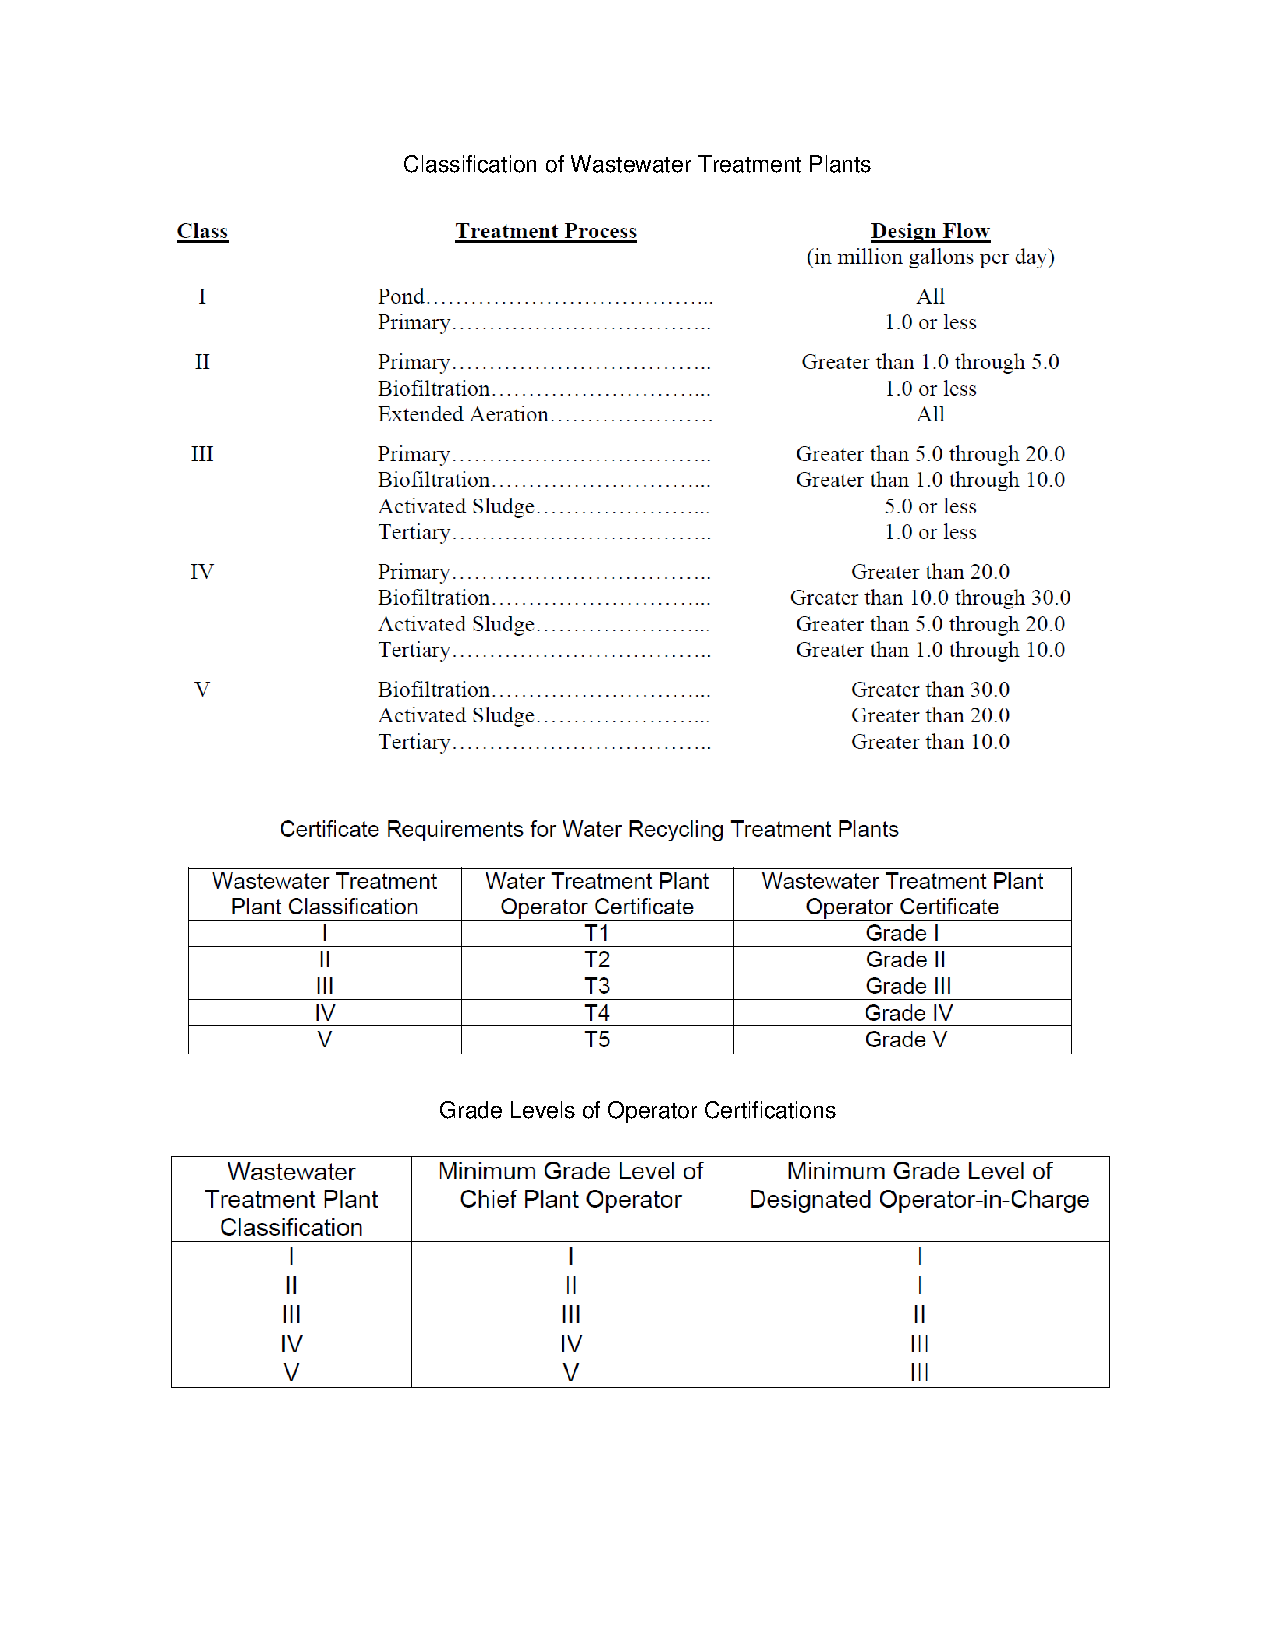
\includepdf[pages=-]{WastewaterPlantOperatorClassificationRequirements.pdf}
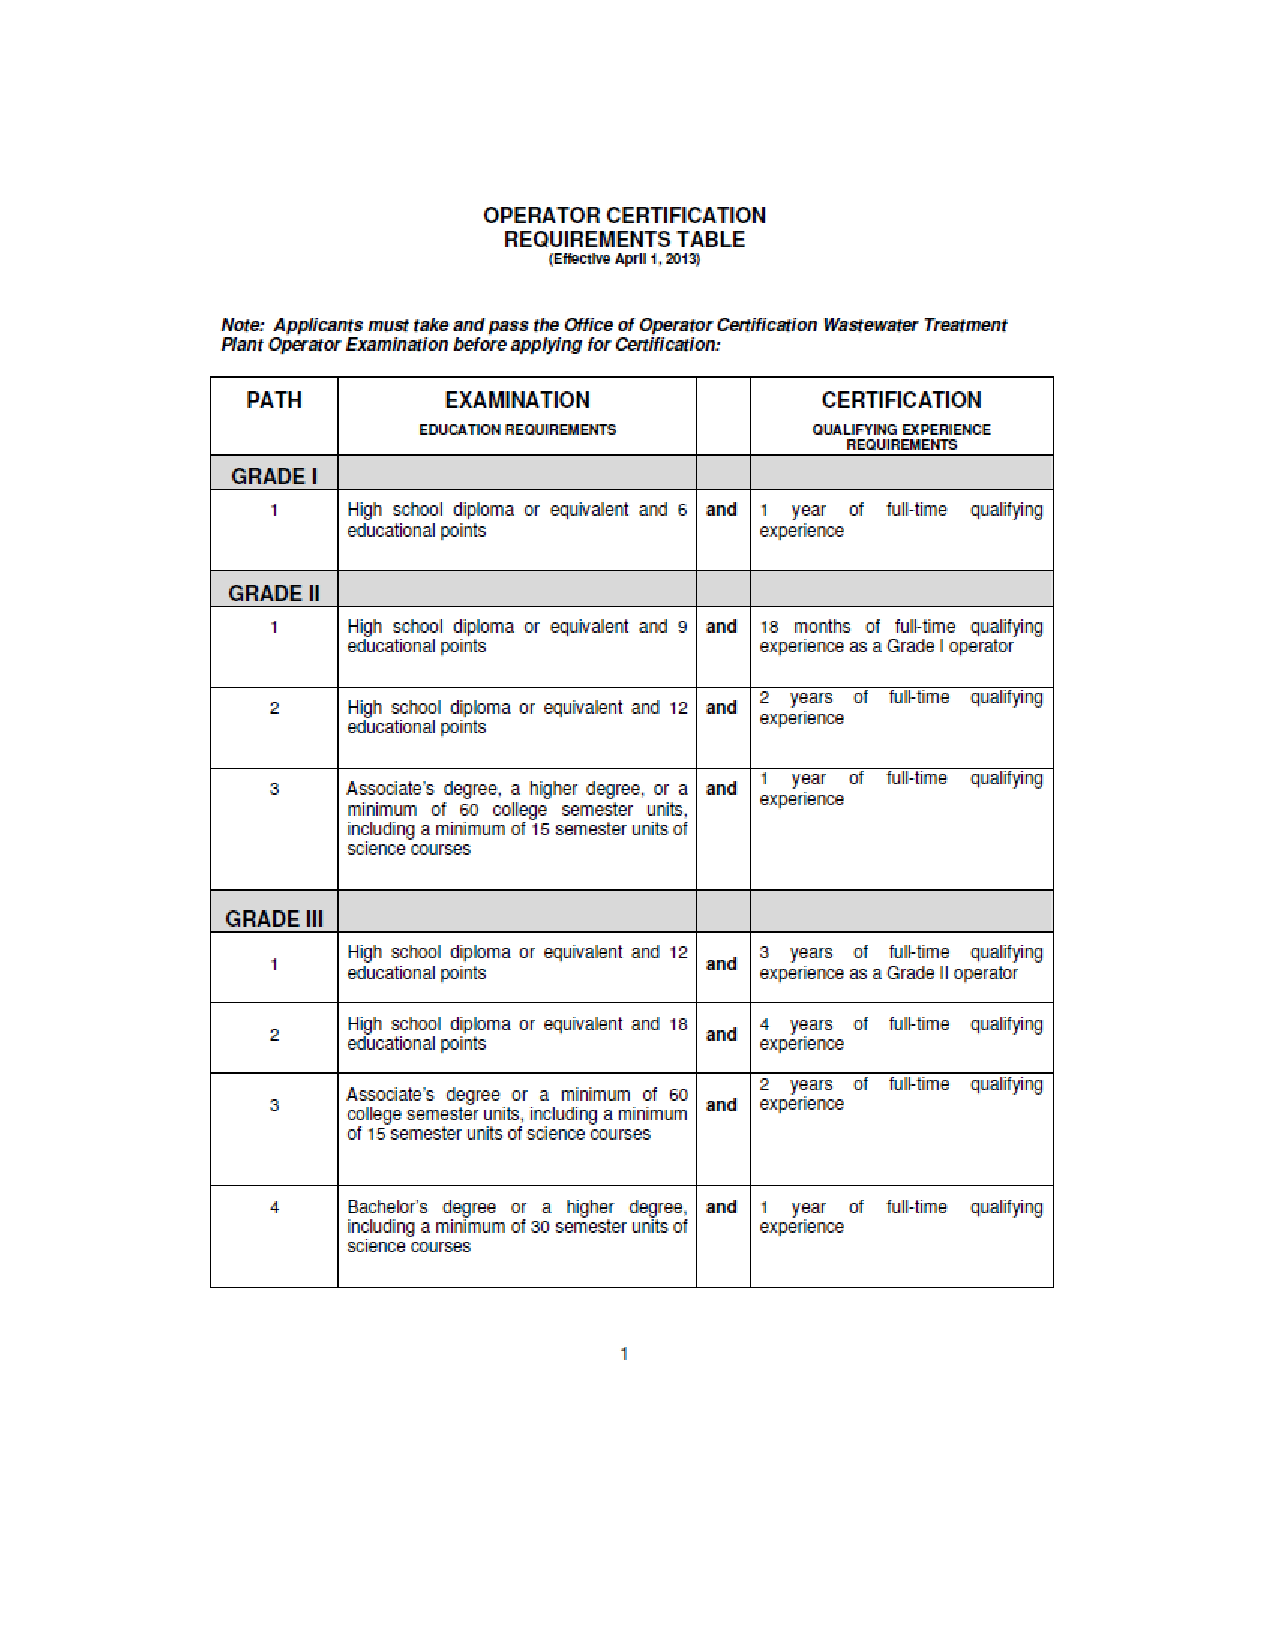
\includepdf[pages=-]{CertificationRequirement.pdf}

\subsection{Worker Safety}\index{Worker Safety}
\begin{itemize}
\item Wastewater treatment facility can be an extremely unsafe occupational field
\item It involves most of the major categories of workplace hazards:  biological, chemical, physical, safety and ergonomic,  accentuated with other factors such as shift work and diverse tasks.
\item Entities including The Occupational Safety and Health Administration(OSHA) National Electrical Code (NEC), National Fire Protection Association (NFPA), Underwriters Laboratory (UL) have recognized these hazards and implemented codes and standards to protect the affected persons and wastewater workers.
\end{itemize}

%\chapterimage{ElementsofTreatmentImg.png} % Chapter heading image
\chapter{Elements of Wastewater Treatment}

Wastewater cycle is a part of the water cycle where the water consumed as part of the normal human and industrial activity is returned back to the environment after treatment.

Wastewater cycle comprises of the following sequential elements:
\begin{enumerate}
\item Generation
\item Collection
\item Treatment
\item Disposal or reuse
\end{enumerate}

\section{Generation}\index{Generation}

Wastewater originates from domestic, industrial, commercial or agricultural activities. The characteristics of wastewater vary depending on the source. Types of wastewater include: 
\begin{itemize}
\item \hl{Domestic Sewage:}  wastewater derived principally from dwellings, business buildings, institutions, and \\
\item \hl{Industrial Sewage:}  liquid waste from industrial processes\\
\end{itemize}
Typical per person generation of wastewater in the USA is about 70-100 gallons per day

\section{Collections}\index{Collections}

\begin{itemize}
\item Wastewater is collected from its point of origin - home, businesses, industries etc. and conveyed via sewer lines to a centralized wastewater treatment facility.  
\item When the rainwater drainage is made part of the sewer system, the system is termed as \hl{Combined System}.  
\item The system where the sewage is conveyed separately from the stormwater flows is termed as \hl{Separated System}.  
\item In the Separated System, the Sanitary Sewers convey the wastewater and the Stormwater Sewer conveys the storm water flows.  
\item For the Combined System, rainstorms pose the threat of overwhelming the sewers and the treatment plant
\end{itemize}  
\begin{center}
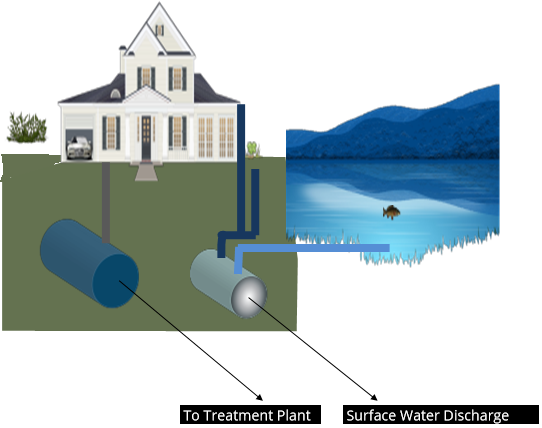
\includegraphics[scale=0.45]{SeperatedSystem1} \hspace{1 cm} 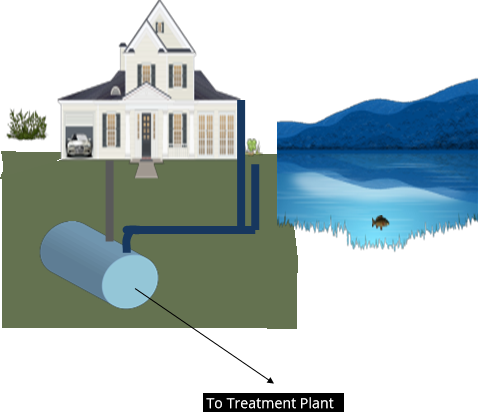
\includegraphics[scale=0.45]{CombinedSystem1}
\end{center}
			\hspace{2.6cm} Separated System \hspace{3.2cm} \parbox{\textwidth}{Combined System}\\

\section{Treatment}\index{Treatment}
\subsection{Liquid Phase Treatment}\index{Liquid Phase Treatment}
\begin{itemize}
\item Wastewater treatment can involve physical, chemical or biological processes or combinations of these processes depending on the required outflow standards. 
\item Wastewater treatment typically involves a series of steps with increasing level of treatment:
\begin{itemize}
\item \hl{Preliminary}:  The preliminary process removes large/coarse solids which include rocks, tree branches, grit and other debris present in wastewater.
\item \hl{Primary}:  The primary process is also a physical process where the separable wastewater solids - solids that float and solids that can settle, are removed.  
\item \hl{Secondary}:  Secondary treatment is a biological treatment process where microorganisms consume the organic matter present in the wastewater. 
\item \hl{Tertiary or Advanced Treatment}:  The tertiary/advanced treatment processes improve the quality of treated water beyond the secondary treatment level.  This process may include nutrient removal and disinfection.
\end{itemize}

\subsection{Treatment of Wastewater Solids}\index{Treatment of Wastewater Solids}
\begin{itemize}
\item Solids are a byproduct of wastewater treatment.  
\item Screenings and grit removed as part of the preliminary treatment is typically disposed in a landfill.
\item Sludge generated from the wastewater treatment processes -  settled solids and scum from primary and secondary treatment processes needs to be treated prior to disposal or reuse to comply with wastewater solids - biosolids regulations.
\end{itemize}

\vspace{0.5cm}
Typical solids treatment is comprised of the following three sequential steps:
\begin{enumerate}
\item Sludge thickening
\item Sludge stabilization
\item Sludge dewatering
\end{enumerate}
\vspace{0.5cm}
\subsubsection{Sludge Thickening}\index{Sludge thickening}
Sludge thickening improves performance of sludge stabilization process and provides capital and operational cost savings due to a lower volume of sludge
\subsubsection{Sludge Stabilization}\index{Sludge Stabilization}
Sludge stabilization process produces solids (biosolids) that meet Part 503 rule requirements. 
\subsubsection{Sludge Dewatering}\index{Sludge Dewatering}
Solids stabilized using digestion process has only a small percentage by weight of solids -less than 5\%.  It therefore becomes necessary to dewater the stabilized sludge prior to hauling off-site for final disposal. 
\vspace{0.5cm}
A generalized layout/process sequencing in a wastewater treatment plant is shown below:
\begin{center}
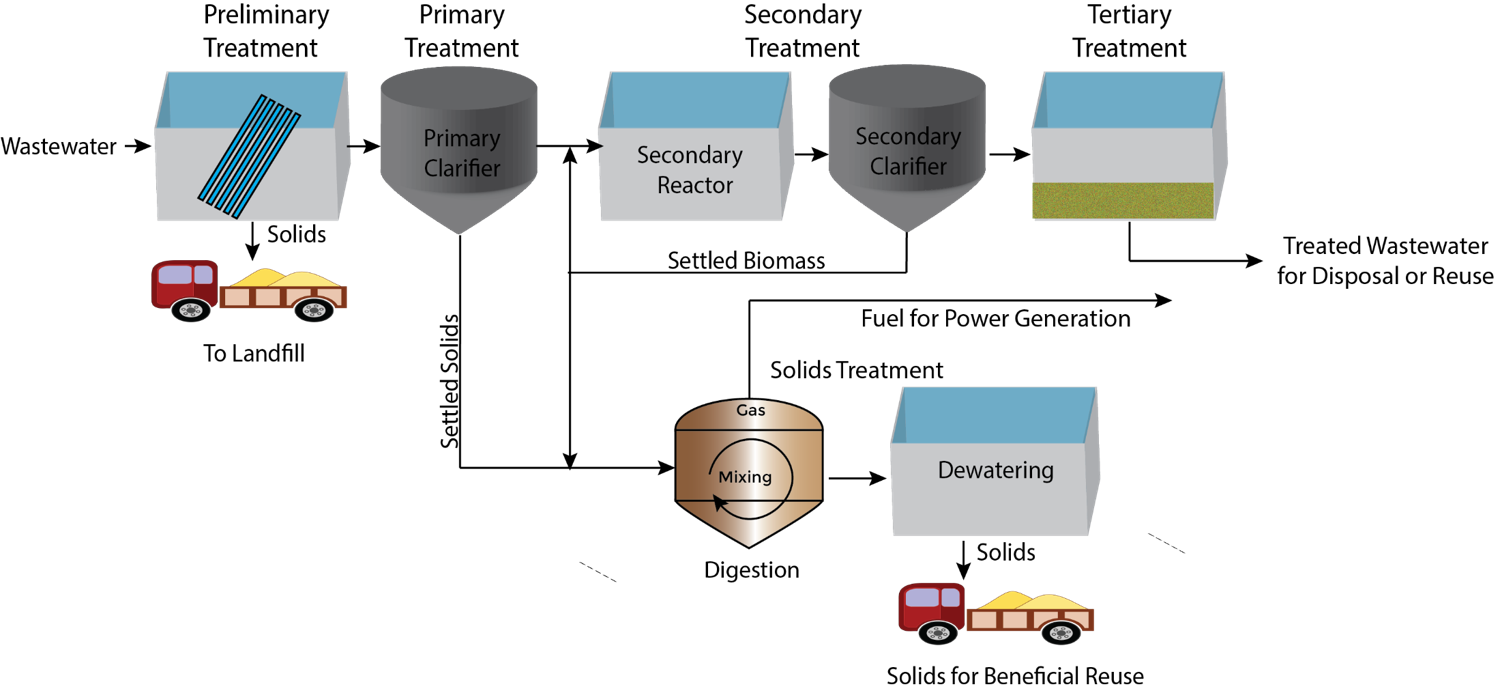
\includegraphics[scale=0.6]{TreatmentFlow}
\end{center}
Individual wastewater treatment processes involve different process options or sequences which are illustrated in the graphic below:
\begin{center}
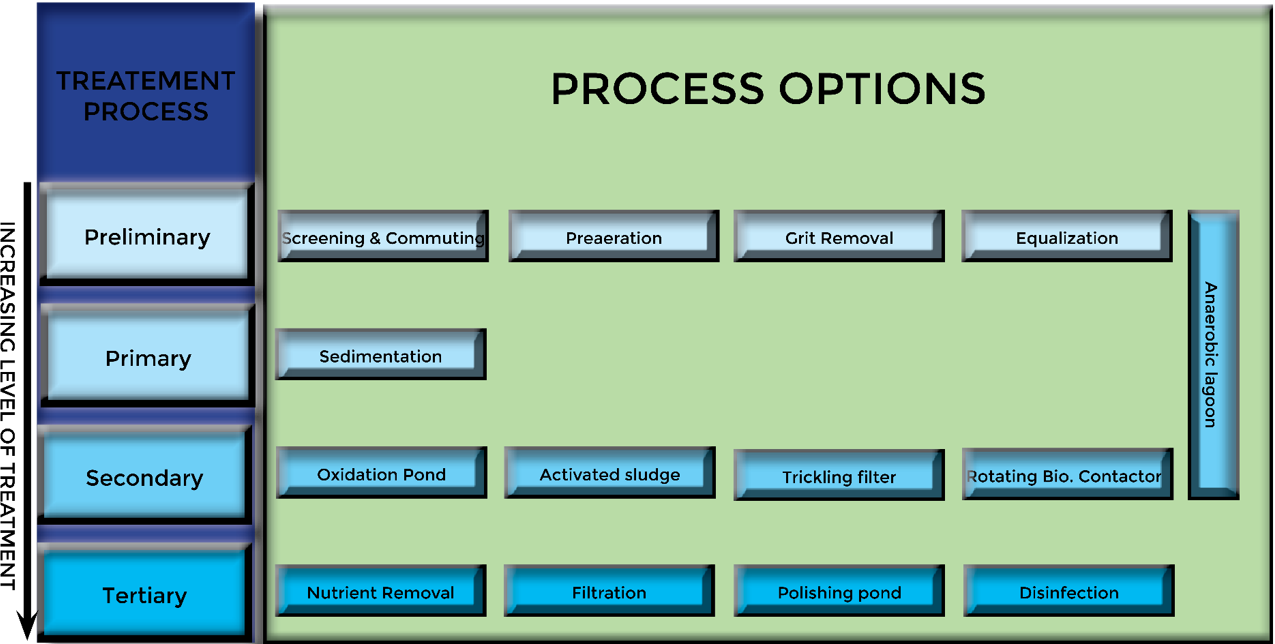
\includegraphics[scale=0.42]{Treatment}
\end{center}
\end{itemize}

\section{Disposal or Reuse}\index{Disposal or Reuse}

\begin{itemize}
\item Wastewater treatment processes can be designed to \hl{dispose} the treated water where the water is reintroduced to the environment or for \hl{reuse} where the treated water is \hl{reclaimed} or \hl{recycled} - for various purposes including irrigation, industrial use or for potable use.
\item Water disposal methods include:\\
\begin{itemize}
\item \hl{Surface water discharge}
\item \hl{Subsurface discharge}
\end{itemize}
\item Water reuse methods include:\\
\begin{itemize}
\item Potable water reuse
\begin{itemize}
\item \hl{Indirect potable reuse:}  Here the treated water is blended with groundwater or surface water and then reclaimed and treated further 
for drinking (potable) water use
\item \hl{Direct potable reuse:}  Here the treated wastewater is subjected to advanced treatment and introduced directly into a municipal water supply system
\end{itemize}
\item Water reclamation for irrigation or industrial use\\
\item Land application for beneficial use\\
\end{itemize}
\item Solids generated from the wastewater treatment process may be removed and disposed to a landfill or subject to further treatment which may allow for energy recovery - from the organic solids and for beneficial reuse due to its plant nutrient content.\\
\end{itemize}


\chapterimage{QuizCover} % Chapter heading image

\chapter{Constituents Properties and Analysis Assessment}
% \textbf{Multiple Choice}

\section*{Constituents Properties and Analysis Assessment}

\begin{enumerate}

\item Positive ORP indicates the presence of an {\underline{\hspace{1cm}}} environment \\

\item {\underline{\hspace{1cm}}} is the predominant microorganism responsible for biological wastewater treatment processes \\

\item MPN is a statistics based method to estimate the concentration of viable bacteria is wastewater and it stands for {\underline{\hspace{1cm}}} \\

\item Describe the three types of composite sampling and explain in your own words on how the sampling would be conducted for each of those methods\\

\item Alkalinity helps in \rule{1.5cm}{0.3mm}control when organic acids are formed as a result of microbiological activity\\

\item Nitrogen in wastewater is typically present as \rule{1.5cm}{0.3mm} and \rule{1.5cm}{0.3mm}\\

\item Volatile solids is determined by incinerating the solids at \rule{1.5cm}{0.3mm} deg. C in a \rule{1.5cm}{0.3mm}

\item  What would be the expected BOD concentration in the wastewater if per capita (person) generation is 0.15lb BOD per day per person and each person produces 80 gallons per day?\\
(Hint: The answer is going to be in mg BOD/l. So multiply lb per day per person by the inverse of dallons per day - so that the unit is lbs per gallon and then convert that to mg/l)\\


\item  Describe the three types of composite sampling and explain in your own words on how the sampling would be conducted for each of those methods \\


\item  tBOD = \rule{.5cm}{0.3mm}BOD + \rule{0.5cm}{0.3mm}BOD

\item  BOD stands for \\

\item  Alkalinity helps in {Nderline{hspace{1cm}}} control when organic acids are formed as a result of microbiological activity \\

\item  Nitrogen in wastewater is typically present as {\underline{\hspace{1cm}}} and {\underline{\hspace{1cm}}} \\


\item  Volatile solids is determined by incinerating the solids at {\underline{\hspace{1cm}}} [temp] deg. C in a {\underline{\hspace{1cm}}} [equipment] 

\item How does one estimate the wastewater sample size used for BOD testing \\

\item Explain how is the nBOD quantified \\

\item Explain why coliforms and enterococcus are used for wastewater bacteriological testing \\

\item What is MPN and why is it used. \\

\item Explain the steps involved in the MTF method\\

\item What is the difference between volatile solids (VS) and volatile suspended solids (VSS) \\

\item Solids that can be used as food by microorganisms \\

\item Test method for determining total ammonium and organic nitrogen content: \rule{0.5cm}{0.3mm}\\

\item Inorganic solids are also called \rule{0.5cm}{0.3mm}\\

\item Oxygen in an anoxic environment is present as {\underline{\hspace{1cm}}} \\

\item Conductivity is the measure of {\underline{\hspace{1cm}}} solids \\

\item Negative ORP signifies {\underline{\hspace{1cm}}} environment \\

\item Alkalinity helps in \rule{0.5cm}{0.3mm} control when organic acids are formed as a result of microbiological activity \\

\item  An Imhoff cone is often used to measure the effectiveness of primary sedimentation. \\

a. True \\
*b. False 

\item  At a primarily domestic wastewater treatment plant, the influent wastewater BOD is always greater than its chemical oxygen demand. \\

a. True \\
*b. False 

\item  Dissolved oxygen in wastewater usually is referred to as combined oxygen. \\

a. True \\
*b. False 

\item  Domestic wastewater generally contains only about 0.1% of solids. \\

*a. True \\
b. False 

\item  Grab or composite samples may be used interchangeable, whichever is most convenient and safest for all laboratory tests. \\

a. True \\
*b. False 

\item  Wastewater with a pH of 12.0 to 14.0 would be too "acidic" for biological treatment. \\

*a. True \\
b. False 

\item  Pre-aeration improves settleability in primary clarifier \\

*a. True \\
b. False 

\item  Total solids are made up of dissolved and suspended solids both of which contain organic and inorganic matter \\

*a. True \\
b. False 

\item  pH value less than 7 indicates an alkaline or basic condition \\

a. True \\
*b. False 

\item  Conductivity is a very useful test for assessing sea water intrusion into sewer lines \\

*a. True \\
b. False 


\item  Sample obtained for wastewater bacteriological testing is typically a composite sample \\

a. True \\
*b. False 

\item  Samples collected for the analysis of COD, BOD, and pH should be acidified for preservation. \\

a. True \\
*b. False 

\item  The MPN test is used to measure pathogen concentrations in wastewater. \\

a. True \\
*b. False 

\item  The total solids in wastewater would be the combination of the fixed solids and the settleable solids. \\

a. True \\
*b. False 

\item  Wastewater with a pH of 2.0 to 4.0 would be too "basic" for biological treatment. \\

a. True \\
*b. False 

\item  Match the measurement units for each of the following: 

\item  The MPN test measures the number of pathogens in a wastewater sample \\

a. True \\
*b. False 

\item  The values of organic matter present in wastewater as measured by BOD and COD tests are typically almost identical \\

a. True \\
*b. False 

\item  In order to obtain valid results in coliform testing, the sample must be dechlorinated at the time of its collection. \\

*a. True \\
b. False 

\item  A flow of 100 gallons per capita per day is often used for estimating flow into a wastewater treatment plant. \\

*a. True \\
b. False 

\item  An Imhoff cone is used to measure settleable solids in units of mg/l. \\

a. True \\
*b. False 

\item  A standardized method exists for the measurement of floatable solids. \\

a. True \\
*b. False 

\item  In the test for coliform bacteria, samples are incubated for 5 days at 20 deg. C. \\

a. True \\
*b. False 

\item  Coliform group organisms are found only in wastewater. \\

a. True \\
*b. False 

\item  Where highly colored samples are involved, the determination of pH by use of a pH meter rather than by color-comparison is\\
preferred. \\

*a. True \\
b. False 

\item  What comes into a treatment plant must go out. This is the basis of the solids balance concept. \\

*a. True \\
b. False 

\item  Receiving water measurements are used to determine the effect of the plant's waste discharge on the receiving waters; therefore, it is necessary to measure both stream and plant\\
effluent characteristics. \\

*a. True \\
b. False 

\item  There are two types of samples that may be collected. One is called an integrated sample, and the other is referred to as a composite. \\

a. True \\
*b. False 

\item  Coliform testing is typically conducted on a grab sample \\

*a. True \\
b. False 

\item  Typical domestic wastewater BOD content is about 2000mg/l \\

a. True \\
*b. False 

\item  BOD is a measure of the organic content of wastewater \\

*a. True \\
b. False 

\item  ORP measurements can be used for controlling the disinfection process \\

*a. True \\
b. False 

\item  MPN is used for enumerating wastewater bacteria and it stands for Measured Pathogen Number \\

a. True \\
*b. False 

\item  For measuring dissolved oxygen in wastewater, it is advisable to use a composite sample \\

*a. True \\
b. False 

\item  A sample to be used for pH measurements should be preserved by the addition of an acid prior to its analysis in the laboratory \\

a. True \\
*b. False 

\item  BOD is a measure of the organic content of wastewater and it stands for Biological Oxidation Demand \\

a. True \\
*b. False 

\item  Conductivity is measured in the units of millivolts using an electrochemical probe \\

a. True \\
*b. False 

\item  Conductivity measurements provide an indirect way to measure total solids present in wastewater \\

a. True \\
*b. False 

\item  Typical wastewater TSS concentrations are in the 2,000-2,500 mg/l range \\

a. True \\
*b. False


\item  A 24-hr flow proportioned sample may be collected for a fecal coliform test\\

a. True \\
*b. False 

\item  Wastewater with a pH of 12.0 to 14.0 would be too "acidic" for biological treatment.\\

*a. True \\
b. False 

\item  The laboratory measurement of volatile solids is a fair approximation of the organic content of the wastewater.\\

*a. True \\
b. False 

\item  BOD5 and SS are both used to measure the strength of wastewater\\

*a. True \\
b. False 

\item  Pre-aeration improves settleability in primary clarifier\\

*a. True \\
b. False 

\item  pH value less than 7 indicates an alkaline or basic condition\\

a. True \\
*b. False 

\newpage
\item A BOD test is run on a secondary effluent.  The data for this test are given below.  Assuming that the average BOD test result for an “inhibitor” on this same secondary effluent was 22 mg/L (cBOD), calculate the oxygen demand caused by nitrification.  What percentage of the total BOD is the nitrogenous oxygen demand?  On April 04, 2009 Exam
  \begin{flalign*}
      Sample Volume, ml     && 50   &&  75  && Blank\\
      \hline
      Initial DO, mg/l      && 9.0  &&  8.9 && 9.2\\
      Final DO, mg/l      && 3.5  &&  1.2 && 9.0
  \end{flalign*}

\begin{itemize}
\item Solution:
  \begin{flalign*}
      Difference, mg/l      &&5.5   &&7.7 &&9.0\\
      tBOD, mg/l          && 5.5*300/50=33 && 7.7*300/75 = 30.8\\
  \end{flalign*}
Average: $\frac{(33 + 30.8)}{2} = 31.9\frac{mg}{l}$\\
$tBOD = cBOD + nBOD \implies 31.9=22 \enspace + \enspace nBOD \implies nBOD=9.9$\\
$\% nBOD = 9.9/31.9 *100 = \boxed{31\%}$
\end{itemize}
\pagebreak
\item BOD tests are run on the final effluent from an activated sludge plant with and without the use of a "nitrification inhibitor". Three hundred milliliter bottles (300 ml) are used in these tests. The raw data for these tests are presented below.  What is the average NITROGENOUS BOD (NBOD)? Exam on April 04, 2009\\
BOD Test without "inhibitor" (tBOD)\\
\begin{flalign*}
      Sample Volume, ml     && 30   &&  60  && Blank\\
      \hline
      Initial DO, mg/l      && 9.0  &&  8.7 && 9.1\\
      Final DO, mg/l      && 5.1  &&  1.2 && 9.0
  \end{flalign*}
BOD Test with "inhibitor" added (cBOD)\\
\begin{flalign*}
      Sample Volume, ml     && 30   &&  60  && Blank\\
      \hline
      Initial DO, mg/l      && 9.0  &&  8.7 && 9.1\\
      Final DO, mg/l      && 6.5  &&  3.5 && 9.0
  \end{flalign*}
\begin{itemize}
\item Solution:
  \begin{flalign*}
      tBOD \\
      Diff., mg/l       &&3.9   &&7.5 &&0.1\\
      tBOD, mg/l          && 3.9*300/30=39 && 7.5*300/60 = 37.5\\
      cBOD \\
      Diff., mg/l       &&2.5   &&5.2 &&0.1\\
      tBOD, mg/l          && 2.5*300/30=25 && 5.2*300/60 = 26\\
  \end{flalign*}

Average:\\
tBOD: $\frac{(39 + 37.5)}{2} = 38.3\frac{mg}{l}$\\
cBOD: $\frac{(25 + 26)}{2} = 25.5\frac{mg}{l}$\\
$tBOD = cBOD + nBOD \implies 38.3=25.5 \enspace + \enspace nBOD \implies nBOD=\boxed{12.8 \frac{mg}{l}}$\\

\end{itemize}
\pagebreak
\item Calculate the TSS of the secondary effluent given the following:\\
\begin{table}[!htbp]
\fontsize{11}{9}
\centering
\begin{tabular}{p{5cm}  p{2cm}}
\hline
\hline
Sample volume& 41 ml \\ [0.2ex] 
\hline
Tare weight of filter \enspace sample & 1.4604 gm \\ 
\hline
Filter + dried residue & 1.4722 gm\\ 
\hline
\hline
\end{tabular}
\end{table}

\item The technician quickly pours 41 ml of well mixed influent into the filter funnel.  The tare weight of the filter is 1.4604 gm. After rinsing, drying, cooling, and weighing, the first dry weight is 1.4722 gm. The filter is returned to the oven and dried, cooled, and weighed. The second dry weight is 1.4700 gm.  Calculate the TSS.

\begin{itemize}
\item Solution\\
$\frac{(1.4722-1.4604)gm \enspace TSS}{41ml}*1000\frac{mg}{gm}*\frac{1000ml}{l}=\boxed{288\frac{mg}{l}}$
\end{itemize}
\newpage
\item BOD tests are run on the final effluent from an activated sludge plant with and without the use of a "nitrification inhibitor". Three hundred milliliter bottles (300 ml) are used in these tests. The raw data for these tests are presented below.  What \textbf{percentage of the average total BOD is the average nBOD}? (10 points)\\
\begin{flalign*}
      Sample Volume, ml     && 10   &&  20  && 30 && 40 && Blank\\
      \hline
      Initial DO, mg/l      && 9.0  &&  8.9 && 8.8  && 9.1 && 9.1\\
      Final DO, mg/l      && 6.9  &&  4.8 && 2.5 && 1.1 && 9.0
  \end{flalign*}
BOD Test with "inhibitor" added (cBOD)\\
\begin{flalign*}
      Sample Volume, ml     && 10   &&  20  && 30 &&  40 && Blank\\
      \hline
      Initial DO, mg/l      && 8.9  &&  8.9  && 9.0 && 9.0 && 9.1\\
      Final DO, mg/l      && 7.5  &&  6.2  && 5.0  && 3.3 && 9.0
  \end{flalign*}

Solution:
  \begin{flalign*}
      tBOD Diff., mg/l      &&2.1   &&4.1 &&6.3 &&8\\
      tBOD, mg/l          && 2.1*300/10=63.0 && 4.1*300/20 = 61.5 && 6.3*300/30 = 63.0 && 8.0*300/40 = 60.0 \\
\hline
      cBOD Diff., mg/l      &&1.4   &&2.7 &&4.0 &&5.7\\
      cBOD, mg/l          && [Discard - diff. <2] && 2.7*300/20 = 40.5 && 4.0*300/30 = 40 && 5.7*300/40 = 42.8\\
  \end{flalign*}

$tBOD (avg) = 63+61.5+63+60=61.9 \hspace{1cm} cBOD (avg) = 40.5+40+42.75=41.1$\\
nBOD = tBOD - cBOD $\implies$ nBOD = 61.9-41.1=20.8 $\implies$ nBOD(\%)=20.8/61.9*100=$\boxed{33.6\%}$
\newpage
\item BOD tests are run on the final effluent from an activated sludge plant with and without the use of a "nitrification inhibitor". Three hundred milliliter bottles (300 ml) are used in these tests. The raw data for these tests are presented below.  What is the average NITROGENOUS BOD (NBOD)? Exam on April 04, 2009\\
BOD Test without "inhibitor" (tBOD)\\
\begin{flalign*}
      Sample Volume, ml     && 30   &&  60  && Blank\\
      \hline
      Initial DO, mg/l      && 9.0  &&  8.7 && 9.1\\
      Final DO, mg/l      && 5.1  &&  1.2 && 9.0
  \end{flalign*}
BOD Test with "inhibitor" added (cBOD)\\
\begin{flalign*}
      Sample Volume, ml     && 30   &&  60  && Blank\\
      \hline
      Initial DO, mg/l      && 9.0  &&  8.7 && 9.1\\
      Final DO, mg/l      && 6.5  &&  3.5 && 9.0
  \end{flalign*}

Solution:
  \begin{flalign*}
      tBOD \\
      Diff., mg/l       &&3.9   &&7.5 &&0.1\\
      tBOD, mg/l          && 3.9*300/30=39 && 7.5*300/60 = 37.5\\
      cBOD \\
      Diff., mg/l       &&2.5   &&5.2 &&0.1\\
      tBOD, mg/l          && 2.5*300/30=25 && 5.2*300/60 = 26\\
  \end{flalign*}

Average:\\
tBOD: $\frac{(39 + 37.5)}{2} = 38.3\frac{mg}{l}$\\
cBOD: $\frac{(25 + 26)}{2} = 25.5\frac{mg}{l}$\\
$tBOD = cBOD + nBOD \implies 38.3=25.5 \enspace + \enspace nBOD \implies nBOD=\boxed{12.8 \frac{mg}{l}}$\\

\pagebreak

\item Calculate percent total solids and percent volatile solids of a sludge sample given the following data:\\
\begin{tabular}{m {5 cm} m {0.5 cm} m  {3.5 cm}}
Weight of dish &=&  104.55 gms\\
Weight of dish and wet sludge &= & 199.95 gms\\
Weight of dish and dry sludge &= & 108.34 gms\\
Weight of dish and ash &= & 106.37 gms
\end{tabular}\\
(Answer: TS = 3.97\%.  VS = 52\%)\\
\vspace{0.2cm}
Solution:\\
\vspace{0.2cm}
Weight of dish=104.55 gms\\
Weight of dish and wet sludge=199.95 gms\\
Weight of dish and ash = 106.37 gms\\
\vspace{0.2cm}
$ \implies Weight \enspace of \enspace sludge=199.95-104.55=95.40 \enspace gms$\\
$\implies Weight \enspace of \enspace dry \enspace sludge \enspace (solids)=108.34-104.55=3.79 \enspace gms$\\
$\implies Weight \enspace of \enspace volatile \enspace solids=108.34-106.37=1.97 \enspace gms$\\
\vspace{0.2cm}
$Total \enspace solids (TS\%)=\frac{gms \enspace solids}{100 \enspace gms \enspace sludge}=\frac{3.79}{95.40} \enspace \frac{gms \enspace solids}{\cancel{gms \enspace sludge}}*\frac{100 \cancel{\enspace gms \enspace sludge}}{100 \enspace gms \enspace sludge}=\boxed{3.97\%}$\\
\vspace{0.2cm}
$Total \enspace volatile \enspace solids (VS\%) =\frac{1.97}{3.79} \enspace \frac{gms \enspace volatile \enspace solids}{\cancel{gms \enspace total \enspace solids}}*\frac{100 \cancel{\enspace gms \enspace total \enspace solids}}{100 \enspace gms \enspace total \enspace solids}=\boxed{52.0\%}$\\
\newpage

\item What is percent volatile solids of a sludge sample given the following data:\\
\begin{tabular}{m {5 cm} m {0.5 cm} m  {3.5 cm}}
Weight of dish &=&  130.69 gms\\
Weight of dish and wet sludge &= & 249.94 gms\\
Weight of dish and dry sludge &= & 134.74 gms\\
Weight of dish and ash &= & 132.05 gms
\end{tabular}\\
\vspace{0.2cm}
Solution:\\
\vspace{0.2cm}
Weight of dish=130.69 gms\\
Weight of dish and wet sludge=249.94 gms\\
Weight of dish and ash = 132.05 gms\\
\vspace{0.2cm}
$ \implies Weight \enspace of \enspace sludge=249.94-130.69=119.25 \enspace gms$\\
$\implies Weight \enspace of \enspace dry \enspace sludge \enspace (solids)=134.74-130.69=4.05 \enspace gms$\\
$\implies Weight \enspace of \enspace volatile \enspace solids=134.74-132.05=2.69 \enspace gms$\\
\vspace{0.2cm}
$Total \enspace solids (TS\%)=\frac{gms \enspace solids}{100 \enspace gms \enspace sludge}=\frac{4.05}{119.25} \enspace \frac{gms \enspace solids}{\cancel{gms \enspace sludge}}*\frac{100 \cancel{\enspace gms \enspace sludge}}{100 \enspace gms \enspace sludge}=\boxed{3.4\%}$\\
\vspace{0.2cm}
$Total \enspace volatile \enspace solids (VS\%) =\frac{2.69}{4.05} \enspace \frac{gms \enspace volatile \enspace solids}{\cancel{gms \enspace total \enspace solids}}*\frac{100 \cancel{\enspace gms \enspace total \enspace solids}}{100 \enspace gms \enspace total \enspace solids}=\boxed{66.4\%}$\\
\newpage
\item Products that are non-biodegradable will have {\underline{\hspace{1cm}}} as compared with biodegradable products \\

a. Same BOD \\
*b. A lower BOD \\
c. A higher BOD \\
d. There is no relationship between BOD and biodegradability 

\item Coliform bacteria are \\

a. Algae \\
b. Coagulant aids \\
*c. Indicators \\
d. Sequestering agents 



\item What is percent volatile solids of a sludge sample given the following data:\\
Weight of dish = 130.69 gms\\
Weight of dish and wet sludge = 249.94 gms\\
Weight of dish and dry sludge = 134.74 gms\\
Weight of dish and ash = 132.05 gms \\

*a. 38.3\% \\
b. 66.4\% \\
c. 42.6\% \\
d. 58.0\% 

\item What is percent volatile solids of a sludge sample given the following data:\\
Weight of dish = 130.69 gms\\
Weight of dish and wet sludge = 249.94 gms\\
Weight of dish and dry sludge = 134.74 gms\\
Weight of dish and ash = 132.05 gms\\

*a. 38.3\% \\
b. 66.4\% \\
c. 42.6\% \\
d. 58.0\% 

\item A device called an Imhoff cone is commonly used to measure settleable solids in: \\

a. \% \\
*b. mL/L \\
c. mg/L \\
d. ppm \\
e. SVI units 

\item An aerobic treatment process is one that requires the presence of: \\

a. Ozone \\
b. organic oxygen \\
c. no oxygen \\
d. combined oxygen \\
*e. dissolved oxygen 

\item A pH probe: \\

a. Can be used to measure ORP in chlorine disinfection. \\
b. Is often used to measure hydrogen production in wet wells. \\
c. Measures, in millivolts, the difference between oxidants like chlorine and reductants such as organic matter. \\
*d. Measures hydrogen ion activity in wastewater. \\
e. Sends a 4-20 mA signal directly to a chlorine controller. 

\item Sludge solids in wastewater has an average specific gravity of 1.2; this means they are \\

a. 12\% heavier than water \\
*b. 20\% heavier than water \\
c. 2\% lighter than water \\
d. 20\% lighter than water 

\item How should the pH electrode be stored when not in use: \\

a. In a strong acid solution \\
b. In a strong caustic solution \\
c. In a safe place in a drawer \\
*d. In distilled water \\
e. In a detergent 

\item In the normal Winkler test: \\

a. A snow white precipitate forms in direct proportion to the nitrate concentration \\
b. A brownish flocculant precipitate is evidence that D.O. is absent \\
c. An endpoint is reached when a dark blue color changes to black \\
d. The muffle furnace must be in excess of 500 deg. C before incubation \\
*e. A snow white precipitate forms if DO is absent 

\item Organisms in wastewater that are not harmful to humans but are indicators of diseases are: \\

a. Pathogens \\
b. Viruses \\
*c. Coliform \\
d. Bacteria 

\item The typical range of suspended solids in domestic influent wastewater is: \\

*a. 100-300 mg/L \\
b. 400-600 mg/L \\
c. 700-900 mg/L \\
d. 1000-12000 mg/L 

\item Which of the flowing statement(s) is/are true with regards to BOD\\
i) BOD test results are suitable for quickly establishing process efficiencies\\
ii) BOD value is always greater than the COD value of the same wastewater sample\\
iii) BOD is expressed in mg/ L or in ppm\\
iv) BOD is the measure of organic strength\\
v) BOD stands for biological oxygen demand \\

a. i) \& ii) \\
b. i), ii) \& iv) \\
c. i), iv) \& v) \\
*d. iii) \& iv) \\
e. iii), iv) \& v) 

\item An amperometric titrater is used to measure \\

a. Alkalinity \\
*b. Chlorine residual \\
c. Conductivity \\
d. COD. 

\item Which of these pH readings indicates an acidic wastewater? \\

*a. 3 \\
b. 7 \\
c. 9 \\
d. 12 

\item Which of the following conditions will probably cause the greatest change in pH? \\

a. Buffering sample \\
*b. Exposing sample to atmosphere \\
c. Fixing sample \\
d. Refrigerating sample 

\item {Nderline{hspace{1cm}}} matter in wastewater, is normally composed of grit, sand and silt. \\

a. Colloidal \\
*b. Inorganic \\
c. Organic \\
d. Volatile 

\item Which of the following characteristics would be least helpful to an operator assessing the organic loading on his plant? \\

a. solids concentration \\
b. BOD \\
c. COD \\
*d. pH \\
e. nitrogen content 

\item Pathogens \\

*a. Are bacteria or virus that cause disease. \\
b. Are bacteria which do not occur in water. \\
c. Can obtain their food supply without help. \\
d. Are not harmful to man. 

\item Regarding the total coliform test which one of the following statements is TRUE? \\

a. If less than 2 coliforms per 100 mL are found in a secondary effluent, we can be assured that we have destroyed all viruses and coliforms. \\
b. Total coliforms are monitored in wastewater because they are generally considered to be disease causing organisms. \\
c. Sodium thiosulfate should be added drop-wise after collection of a coliform sample to destroy residual chlorine. \\
*d. The multiple tube fermentation method for measuring total coliforms is only a statistical estimate of the coliform organism concentration. 

\item Results from the Multiple-Tube Fermentation Technique for members of the Total Coliform Group are expressed as \\

a. DPD. \\
b. MF. \\
c. MGD. \\
*d. MPN. 

\item The advantage in the use of coliform organisms as an indicator lies in the following fact: \\

a. They are found everywhere and they grow in common bacterial media \\
b. They are found everywhere and are readily killed by chlorine \\
*c. They are predominant bacteria associated with intestinal discharges and grow on\\
nutrient agar forming characteristic colonies 

\item The purpose of adding sodium thiosulfate to a microbiological sample bottle is to \\

a. Extend the allowable holding time from 6 to 30 hours. \\
b. React with nitrates that interfere with the MPN test. \\
*c. Remove any chlorine residual present. \\
d. To ensure sterilization of sample bottle. 

\item The solids in a raw wastewater sample may be classified in several different categories. However, one may say that all the solids in a wastewater sample may be expressed as the sum of: \\

a. The total of settleable solids + total dissolved solids. \\
*b. The total dissolved solids + total suspended solids. \\
c. The total of settleable solids + colloidal solids + total suspended solids 

\item The term MPN is used in reference to: \\

a. The mass of phosphorus and nitrogen per unit of carbon \\
*b. The number of coliforms per unit volume of sample that is most likely to have caused the observed results in a multiple tube test \\
c. The number of fecal stetococci per unit volume of sample that is most likely to have caused the observed results in the multiple tube test \\
d. The result of membrane filter test \\
e. The standard plate count result 

\item The volatile portion of suspended solids contained in normal domestic wastewater could be expected to be in the range of \\

a. Less than 10 % • \\
b. 25-50%. \\
*c. 70-80%. \\
d. 90-100%. 

\item What disease is not considered to be normally conveyed or transmitted by untreated wastewater? \\

a. Amoebic dysentery. \\
b. Hepatitis. \\
*c. Malaria. \\
d. Chlorea. 

\item What test is not run on the influent? \\

a. BOD. \\
*b. Fecal coliform. \\
c. Suspended solids. \\
d. pH. 

\item Which one of the following statements is TRUE regarding the standard BOD5 test? \\

a. Some NPDES permits specify that only CBOD is to be reported on a wastewater plant's final effluent. The letters CBOD refer to complete BOD (i.e the TOTAL BOD). \\
b. Phenylarsineoxide (PAD) is typically added to destroy nitrifying bacteria when running this test. \\
c. Dechlorinated secondary effluents need not be seeded when set up for the BODs test. \\
d. Nitrate ions interfere with this test \\
*e. The BOD measured includes the nitrogenous BOD (nBOD).results due to the oxygen demand exerted by certain bacteria as they oxidize ammonia to nitrate ions. 

\item A composite sample will provide a(an) \\

a. Even color. \\
b. High pH. \\
c. Low solids sample. \\
*d. Representative sample. 

\item Flow proportionate composite samples are collected because: \\

a. The waste characteristics are continually changing \\
b. The flow is continually changing \\
*c. The flow and waste characteristics are continually changing \\
d. This requires less time than grab samples \\
e. All of the above 

\item Over a four-year period, the totalizing hour meter on an instrument air compressor had the following readings at the end of each year: 1st year - 9,763; 2nd year - 13,258; 3rd year - 20,071; and 4th year - 23,714 How many hours does the meter show the compressor ran during \\the third year? \\

a. 349.5 hours \\
b. 364.3 hours \\
*c. 681.3 hours \\
d. 830.2 hours 

\item Grab sample is always collected for which of the following test \\

a. BOD \\
b. TSS \\
*c. Coliform \\
d. COD \\
e. None of the above 

\item Samples collected over several hours during the day and combined are known as: \\

*a. Composite samples. \\
b. Grab samples. \\
c. Deep samples. \\
d. Periodic samples. 

\item Grab samples are considered to be representative of the \\

a. Average daily condition at the sample location \\
b. Average daily condition in the system \\
c. System conditions for the two hours before and after the sample was taken \\
*d. System condition at the time of the sample 

\item Characteristics that should be measured immediately after the sample is collected are: \\

a. Velocity and dissolved solids \\
*b. Temperature, pH and DO \\
c. TSS and BOD \\
d. Hardness and alkalinity 

\item A stilling well on the effluent side of a wastewater facility is: \\

a. a chlorine injection concentrator \\
b. an automatic sampler for coliform counts \\
*c. a structure containing the float for a flow measuring device \\
d. dry well side of a pump station \\
e. a none of the above 

\item The advantages of automatic sampling equipment are: \\

a. elimination of human error inherent in manual sampl ing \\
b. reduction of personnel requirements and cost \\
c. allows for more frequent sampling \\
d. collection of more representative samples \\
*e. all of the above 

\item In collecting a sample for a chlorine residual determination of the final effluent, the most suitable sampling point is: \\

a. at the site of chlorine injection \\
b. at the entrance to the chlorine contact chamber \\
c. at the midpoint of the chlorine contact chamber \\
d. at the exit side of the chlorinator \\
*e. at the point of effluent discharge 

\item The recommended minimum portion which should be collected for testing in sampling wastewater is: (Assume a grab sample) \\

a. 10 ml \\
b. 50 ml \\
c. 10 0 ml \\
d. 500 ml \\
*e. 1,000 ml 

\item A composite sample will give a(n) \\

a. Even color \\
b. High pH \\
c. Instantaneous sample \\
*d. Representative sample 

\item Chlorine residual may be determined using the reagent \\

*a. Diethyl-p-phenylenediamine (DPD) \\
b. Ethylendiamine tetraacetic acid (EDTA) \\
c. Polychlorinated biphenyls (PCB) \\
d. Sodium thiosulfate (Na2S203) 

\item BOD5 is the most common method to quantify the organic content in wastewater. Another method used is: \\

a. Chemical oxygen demand \\
b. Volatile solids analysis \\
c. Total organic carbon \\
*d. Any of the above 

\item The laboratory test results on domestic raw sewage were: COD = 320 mg/1 BOD = 475 mg/1. The best interpretation would be: \\

a. the raw wastewater had a high grease content \\
b. the raw wastewater was septic \\
*c. the laboratory results, as reported, were in error \\
d. the sample was held too long before analysis \\
e. the glass fiber filters used to run the test were contaminated 

\item TKN is the measure of: \\

a. Ammonia/Ammonium+Inorganic Nitrogen \\
*b. Ammonia/Ammonium+Organic Nitrogen \\
c. Nitrate+Nitrite+Organic Nitrogen \\
d. Organic Nitrogen+Inorganic Nitrogen 

\item Volatile solids concentration of sludge with 6% solids containing 70% volatile matter is: \\

*a. 42,000mg/l \\
b. 70,000mg/l \\
c. 42mg/l \\
d. 700mg/l 

\item Wastewater solids can be categorized as: \\

a. Suspended+Fixed \\
b. Dissolved+Volatile \\
*c. Volatile+Fixed \\
d. Volatile+Settleable 

\item Non-settleable solids are composed of: \\

a. Volatile +Dissolved \\
b. Dissolved+Settleable \\
c. Floatable + Suspended \\
*d. Collodial + Floatable 

\item Sludge with a specific gravity of 1.1 will weigh: \\

a. 1.1lbs/gal \\
b. 8.34lbs/gal \\
*c. 9.17lbs/gal \\
d. 7.58lbs/gal 



\item  A composite sample will provide a(an) \\

a. Even color. \\
b. High pH. \\
c. Low solids sample. \\
*d. Representative sample. 

\item  Bacteria which cause diseases in man are generally called: \\

a. Mesophilic \\
b. Facultative \\
*c. Pathogenic \\
d. Coliforms 

\item  How should the pH electrode be stored when not in use: \\

a. In a strong acid solution \\
b. In a strong caustic solution \\
c. In a safe place in a drawer \\
*d. In distilled water \\
e. In a detergent 

\item  In the normal Winkler test: \\

a. A snow white precipitate forms in direct proportion to the nitrate concentration \\
b. A brownish flocculant precipitate is evidence that D.O. is absent \\
c. An endpoint is reached when a dark blue color changes to black \\
d. The muffle furnace must be in excess of 500 deg. C before incubation \\
*e. A snow white precipitate forms if DO is absent 

\item  The typical range of suspended solids in domestic influent wastewater is: \\

*a. 100-300 mg/L \\
b. 400-600 mg/L \\
c. 700-900 mg/L \\
d. 1000-12000 mg/L 

\item  Which of the flowing statement(s) is/are true with regards to BOD\\
1) BOD test results are suitable for quickly establishing process efficiencies\\
2) BOD value is always greater than the COD value of the same wastewater sample\\
3) BOD is expressed in mg/ L or in ppm\\
4) BOD is the measure of organic strength\\
5) BOD stands for biological oxygen demand\\

a. 1) and 2) \\
b. 1), 2) \& 4) \\
c. 1), 4) \& 5) \\
*d. 3) \& 4) \\
e. 3), 4) and 5) 

\item  {Nderline{hspace{1cm}}} matter in wastewater, is normally composed of grit, sand and silt. \\

a. Colloidal \\
*b. Inorganic \\
c. Organic \\
d. Volatile 

\item  Pathogens \\

*a. Are bacteria or virus that cause disease. \\
b. Are bacteria which do not occur in water. \\
c. Can obtain their food supply without help. \\
d. Are not harmful to man. 

\item  Regarding the total coliform test which one of the following statements is TRUE? \\

a. If less than 2 coliforms per 100 mL are found in a secondary effluent, we can be assured that we have destroyed all viruses and coliforms. \\
b. Total coliforms are monitored in wastewater because they are generally considered to be disease causing organisms. \\
c. Sodium thiosulfate should be added drop-wise after collection of a coliform sample to destroy residual chlorine. \\
*d. The multiple tube fermentation method for measuring total coliforms is only a statistical estimate of the coliform organism concentration. 

\item  Results from the Multiple-Tube Fermentation Technique for members of the Total Coliform Group are expressed as \\

a. DPD. \\
b. MF. \\
c. MGD. \\
*d. MPN. 

\item  The advantage in the use of coliform organisms as an indicator lies in the following fact: \\

a. They are found everywhere and they grow in common bacterial media \\
b. They are found everywhere and are readily killed by chlorine \\
*c. They are predominant bacteria associated with intestinal discharges and grow on\\
nutrient agar forming characteristic colonies 

\item  The purpose of adding sodium thiosulfate to a microbiological sample bottle is to \\

a. Extend the allowable holding time from 6 to 30 hours. \\
b. React with nitrates that interfere with the MPN test. \\
*c. Remove any chlorine residual present. \\
d. To ensure sterilization of sample bottle. 

\item  The term MPN is used in reference to: \\

a. The mass of phosphorus and nitrogen per unit of carbon \\
*b. The number of coliforms per unit volume of sample that is most likely to have caused the observed results in a multiple tube test \\
c. The number of fecal stetococci per unit volume of sample that is most likely to have caused the observed results in the multiple tube test \\
d. The result of membrane filter test \\
e. The standard plate count result 

\item Describe total coliform \& fecal coliform bacteria.  What is the difference between the two?  Describe the test procedures for both.


Response:\\
\begin{enumerate}[label=\alph*]
\item \textit{Describe total coliform \& fecal coliform bacteria.}
\begin{itemize}
\item Coliform bacteria are a broad group of bacteria found in soil, water and other environments.
\item Fecal coliform are coliforms which originate in the intestines of warm-blooded animals
\end{itemize}
\item \textit{What is the difference between the two? }\\
While total coliforms are found widely in different environments, fecal coliforms are typically found in the intestines of warm blooded animals and are indicators of fecal contamination.
\item \textit{Describe the test procedures for both.}\\
The Multiple Tube Fermentation method to estimate the quantity of both these microorganisms includes the following steps:
\begin{itemize}
\item Conducting a presumptive test by inoculating the sample in a set of 15 tubes containing Lauryl Tryptose Broth each containing an inverted Durham tube followed by incubation and observation of a positive result for each tube indicated by turbidity and presence of gas bubble.
\item Conducting a confirmed test by innoculating each of the positive samples from the presumptive test into a tube containing BGB broth - for Total Coliform and EC Broth - for Fecal Coliform
\item Conducting a completed test by streaking and incubating an agar plate with positives from the confirmed test followed by innoculating and incubating an agar slant and nutrient broth with colonies from the agar plate.


\end{itemize}
\end{enumerate}
\item What is ORP
\vspace{0.3cm}
Response:\\
\vspace{0.3cm}
Oxidation is a chemical reaction in which electrons are gained by oxidizing agent and lost by the substance being oxidized.  Electrons cause bonds to be broken in the organic matter thus destroying it.\\
\vspace{0.5cm}
Oxidation potential is the direct measure in millivolts of demand for chlorine; more chlorine increases oxidants potential more organic matter lowers oxidation potential.\\
Using ORP probe reduces amount of chlorine used for disinfection.  Chlorine by-products are toxic cause problems in effluent toxicity test.\\
\vspace{0.5cm}
ORP (oxidation red\vspace{0.5cm}uction potential) probes have been found to be effective in precisely controlling chlorine disinfection as well as de-chlorination.   An ORP probe measures directly the oxidation potential and compares (his measured potential to a set point (typically 540 mV).  A 4-20 milliamp controller can be used to adjust the chlorine feed to use precisely the amount of chlorine needed for disinfection. 


\item  When chlorine is added to a wastewater effluent it is said to act as an oxidizing agent.  Define oxidation.  Explain how oxidation might be effective in disinfection of a wastewater effluent.\\
\vspace{0.3cm}
Response:\\
\vspace{0.3cm}
Oxidation is a chemical reaction in which electrons are gained by the oxidizing agent and lost by the substance being oxidized.\\
These lost electrons cause bonds to be broken in the organic matter (bacteria) and thus destroy it.
\\
\item Define oxidation potential.   Explain how (his potential changes in relationship to the addition of chlorine or the increase in organic material or bacteria in the wastewater.  
\\
\vspace{0.3cm}
Response:\\
\vspace{0.3cm}Oxidation potential is a direct measure, in millivolts, of the potential for electron transfer to the oxidizing agent (chlorine).  \\
More chlorine increases oxidation potential.  \\
More organic material or bacteria lowers the oxidation potential.\\

\item One WWTP found that it was better able to meet its effluent toxicity limit when using an ORP probe.  Identify and briefly explain one possible reason for this.\\
\vspace{0.3cm}
Response:\\
\vspace{0.3cm}
Using an ORP probe reduces significantly the amount of chlorine being used for disinfection.  \\
Chlorine by-products are often toxic and thus cause problems in the effluent toxicity test (bioassay test).  \\
Reducing the chlorine used may make it easier to meet the toxicity limit.\\


\item An ORP probe must be place several minutes downstream of the point where chlorine is added in a chlorine contact tank.  Why?  Identify the data and conversion factor(s) necessary to calculate where an ORP probe is to be placed.  Assume that at peak dry flow (he probe is to be placed 5 minutes downstream of the point where chlorine is added.  Show the steps necessary to do this calculation.\\
\vspace{0.3cm}
Response:\\
\vspace{0.3cm}
Reactions with ammonia-nitrogen are not instantaneous.  Thus, sometime between the point of addition of chlorine and the site of the ORP probe to allow these reactions to be complete.
Data needed to calculate position of the probe: Peak Flow (MGD), the conversion factor = MGD = 1.547 cu. ft. / sec., the width of the chlorine contact chamber, the depth of the water in the chlorine contact chamber (so that the cross-sectional area of the flow can be calculated), 60 sec = 1 minute.\\

1.  Find the velocity of flow (ft/sec): Q at peak x 1.547 cu. ft./sec divided by cross-sectional area in ft2.
2.  Convert velocity (ft/sec) to ft/min = ft/sec x 60 sec/min = ft/min
3.  Multiply ft/min x 5 min to find ft.









\end{enumerate}






\chapterimage{QuizCover} % Chapter heading image

\chapter{Collections Assessment}
% \textbf{Multiple Choice}

\section*{Collections Assessment}
\begin{enumerate}

\item  Hydrogen sulfide gas in a moist atmosphere can result in corrosion of concrete structures \\

*a. True \\
b. False \\

\item  As a rule of thumb, the velocity in a gravity sewer should be at least 2 cubic feet per second to ensure that the solids do not settle out in the sewer lines\\

a. True \\
*b. False \\

\item  A combined sewer implies that it carries domestic and industrial wastes only \\

a. True \\
*b. False \\

\item  Hydrogen sulfide gas in a moist atmosphere can result in corrosion of concrete structures \\

*a. True \\
b. False \\

\item  Inflow is storm water entering into the sewer system \\

*a. True \\
b. False \\

\item  A combined wastewater collection system handles only domestic waste and industrial waste. \\

a. True \\
*b. False \\

\item  Fats, oils and grease accumulation in sewers can cause sewer overflows \\

*a. True \\
b. False \\

\item  Storms could potentially cause sewer overflows in a Combined Sewer system  \\

*a. True \\
b. False \\

\item  Groundwater entering sewer collection pipes through cracks and defective pipe joints is termed as inflow \\

a. True \\
*b. False \\

\item  A Combined sewer system is the one that brings the combined domestic and industrial wastewater flow to the treatment plant \\

a. True \\
*b. False \\

\item  Infiltration is when groundwater enters the sewage collections systems \\

*a. True \\
b. False \\

\item  Infiltration is when groundwater enters the sewage collections systems \\

*a. True \\
b. False \\

\item  As a rule of thumb, the velocity in a gravity sewer should be at least 2 cubic feet per second to ensure that the solids do not settle out in the sewer lines\\

a. True \\
*b. False \\

\item  A combined sewer implies that it carries domestic and industrial wastes only \\

a. True \\
*b. False \\

\item  Hydrogen sulfide gas in a moist atmosphere can result in corrosion of concrete structures \\

*a. True \\
b. False \\

\item  Inflow is storm water entering into the sewer system \\

*a. True \\
b. False \\



\item  A lateral is the largest sewer line which brings the wastewater to the treatment plant \\

a. True \\
*b. False \\

\item  Hydrogen sulfide gas in a moist atmosphere can result in corrosion of concrete structures \\

*a. True \\
b. False \\

\item  As a rule of thumb, the velocity in a gravity sewer should be at least 2 cubic feet per second to ensure that the solids do not settle out in the sewer lines\\

a. True \\
*b. False \\

\item  A combined sewer implies that it carries domestic and industrial wastes only \\

a. True \\
*b. False \\

\item  Hydrogen sulfide gas in a moist atmosphere can result in corrosion of concrete structures \\

*a. True \\
b. False \\

\item  Inflow is storm water entering into the sewer system \\

*a. True \\
b. False \\

\item  A combined wastewater collection system handles only domestic waste and industrial waste. \\

a. True \\
*b. False \\

\item  Fats, oils and grease accumulation in sewers can cause sewer overflows \\

*a. True \\
b. False \\

\item  Storms could potentially cause sewer overflows in a Combined Sewer system  \\

*a. True \\
b. False \\

\item  Groundwater entering sewer collection pipes through cracks and defective pipe joints is termed as inflow \\

a. True \\
*b. False \\

\item  A Combined sewer system is the one that brings the combined domestic and industrial wastewater flow to the treatment plant \\

a. True \\
*b. False \\

\item  Infiltration is when groundwater enters the sewage collections systems \\

*a. True \\
b. False \\

\item Define Infiltration and Inflow.  Discuss the impact of inflow and infiltration on the wastewater treatment plant:


\item  In wastewater collections what is a gravity system:

\item  A sewer system designed to transport only wastewater from homes, industries, institutions and businesses is called: \\

a. Combined sewer \\
*b. Sanitary sewer \\
c. Service sewer \\
d. Building sewer \\

\item  Velocity of sewers is usually expressed as: \\

*a. Feet per second \\
b. Gallon per minute \\
c. MGD \\
d. mg/l \\
e. sq. ft \\

\item  Which of the following statements is not true regarding a wastewater collection system: \\

*a. A sewer is designed to allow the waste to flow at a rate of approximately 1 ft/sec. \\
b. Grease can be serious problem in a collection system. \\
c. Inflow and infiltration are frequently problems in older collection systems. \\
d. High concentrations of hydrogen sulfide in a sewer can lead to corrosion of concrete. \\
e. Scouring can be a problem if wastewater is flowing too fast. \\

\item  Which of the following statements is not true regarding a wastewater collection system: \\

*a. A sewer is designed to allow the waste to flow at a rate of approximately 1 ft/sec. \\
b. Grease can be serious problem in a collection system. \\
c. Inflow and infiltration are frequently problems in older collection systems. \\
d. High concentrations of hydrogen sulfide in a sewer can lead to corrosion of concrete. \\
e. Scouring can be a problem if wastewater is flowing too fast. \\

\item  A sewer system designed to transport only wastewater from homes, industries, institutions and businesses is called: \\

a. Combined sewer \\
*b. Sanitary sewer \\
c. Service sewer \\
d. Building sewer \\

\item  Velocity of sewers is usually expressed as: \\

*a. Feet per second \\
b. Gallon per minute \\
c. MGD \\
d. mg/l \\
e. sq. ft \\

\item  Velocity of flow in sewers is usually expressed in terms of \\

*a. Feet per second \\
b. Gallon per minute \\
c. MGD \\
d. Milligrams per liter \\
e. Square feet \\

\item  Velocity of flow in sewers is usually expressed in terms of \\

*a. Feet per second \\
b. Gallon per minute \\
c. MGD \\
d. Milligrams per liter \\
e. Square feet \\

\item Infiltration is caused by:
*a. Cracked pipes
b. Improper CCTV operation
c. Poor ventilation
d. All of the above



\item Define infiltration \& inflow, compatible \& non-compatible. List 4 major concerns.  List 2 corrections.


\end{enumerate}
\chapterimage{QuizCover} % Chapter heading image

\chapter{Preliminary Treatment Assessment}
% \textbf{Multiple Choice}

\section*{Preliminary Treatment Assessment}


\begin{enumerate}

\item A weir can be also be used for measuring flows\\

*a. True \\
b. False 
\vspace{0.4cm}
\item The process of pre-aeration in no way influences the degree of settling in a primary clarifier\\
\vspace{0.4cm}
a. True \\
*b. False 
\vspace{0.4cm}
\item Septic sludge has a low pH\\

*a. True \\
b. False 
\vspace{0.4cm}
\item A Parshall flume measures the velocity of the influent flow\\

a. True \\
*b. False 
\vspace{0.4cm}
\item  A barminutor frequently operates automatically. \\

*a. True \\
b. False 

\vspace{0.4cm}
\item  A grit chamber with a faster flow velocity than recommended may allow appreciable organic matter to collect in the grit. \\

a. True \\
*b. False 

\vspace{0.4cm}
\item  A grit chamber with a slower flow velocity than recommended may allow appreciable organics to settle out with the grit. \\

*a. True \\
b. False 

\vspace{0.4cm}
\item  A Parshall Flume is a device used to divide the incoming flow for equal distribution to a plant having more than one primary clarifier. \\

a. True \\
*b. False 

\vspace{0.4cm}
\item  A Parshall flume measures the velocity of the influent flow \\

a. True \\
*b. False 

\vspace{0.4cm}
\item  A properly operated grit chamber will normally increase the solids loading to the primary clarifier \\

*a. True \\
b. False 

\vspace{0.4cm}
\item  A properly operating grit chamber should yield grit that is high in fixed solids (inorganic material) and low in volatile solids. \\

*a. True \\
b. False 

\vspace{0.4cm}
\item  At most treatment plants preliminary treatment is used to protect pumping equipment and to facilitate subsequent treatment processes. \\

*a. True \\
b. False 

\vspace{0.4cm}
\item  A Venturi meter measures the amount of electricity used and should be read when there is a high electrical demand. \\

a. True \\
*b. False 

\vspace{0.4cm}
\item  A weir can be used as a flow measuring device \\

*a. True \\
b. False 

\vspace{0.4cm}
\item  Hydrogen sulfide gas in a moist atmosphere can result in corrosion of concrete structures \\

*a. True \\
b. False 

\vspace{0.4cm}
\item  Inefficient grit removal would tend to cause a decrease in percent volatile solids in raw primary sludge \\

*a. True \\
b. False 

\vspace{0.4cm}
\item  pH value less than 7 indicates an alkaline or basic condition \\

a. True \\
*b. False 

\vspace{0.4cm}
\item  Poor grit removal would affect all of the following: pumps and other mechanical equipment, anaerobic digestion, percent volatile and percent total solids in the raw sludge. \\

*a. True \\
b. False 

\vspace{0.4cm}
\item  Pre-aeration improves settleability in primary clarifier \\

*a. True \\
b. False 

\vspace{0.4cm}
\item  Pre-aeration of raw wastewater may cause better solids separation and removals\\
in the primary clarifier. \\

*a. True \\
b. False 

\vspace{0.4cm}
\item  Presence of hydrogen sulfide cannot always be detected by its characteristic odor \\

*a. True \\
b. False 

\vspace{0.4cm}
\item  In a typical treatment facility, it is necessary to have flow meters on the influent and effluent to detect the loss in plant flow. \\

a. True \\
*b. False 

\vspace{0.4cm}
\item  A Venturi meter is a reliable device for measuring flows of either treated or untreated wastewater. \\

*a. True \\
b. False 

\vspace{0.4cm}
\item  A flow measurement device such as a constant differential meter, or the more common name, rotameter, is used for the measurement of liquids or gases. \\

*a. True \\
b. False 

\vspace{0.4cm}
\item  It is often necessary to pre-chlorinate wastewater to prevent odors. When this is done, it is not necessary to satisfy a chlorine demand or expect a chlorine residual. \\

*a. True \\
b. False 

\vspace{0.4cm}
\item  Inefficient grit removal would tend to cause an increase in the percent volatile solids in raw sludge. \\

a. True \\
*b. False 

\vspace{0.4cm}
\item  Grit is composed mostly of inorganic material and organic material that is not easily biodegradable \\

*a. True \\
b. False 

\vspace{0.4cm}
\item  A weir can be also be used for measuring flows \\

*a. True \\
b. False 

\vspace{0.4cm}
\item  {Nderline{hspace{1cm}}} is used for controlling the flow velocity in a horizontal grit channel \\

Correct Answer(s):\\
a. True\\
b. False 

\vspace{0.4cm}
\item  Septic sludge has a low pH \\

*a. True \\
b. False 

\vspace{0.4cm}
\item  Barminutors and comminutors are devices which cut up or shred material which is normally found in raw wastewater. \\

*a. True \\
b. False 

\vspace{0.4cm}
\item  Barmunitor and comminutor are devices used for cutting up or shredding material normally present in raw wastewater \\

*a. True \\
b. False 

\vspace{0.4cm}
\item  Coliform testing is typically conducted on a grab sample \\

a. True \\
*b. False 

\vspace{0.4cm}
\item  Comminutors cut up or shred large objects normally found In raw wastewater and remove them from the wastewater flow. \\

a. True \\
*b. False 

\vspace{0.4cm}
\item  Conductivity is a very useful test for assessing sea water intrusion into sewer lines \\

*a. True \\
b. False 

\vspace{0.4cm}
\item  Fresh wastewater is characterized by a blackish color, foul and unpleasant odors with floating materials and suspended solids. \\

a. True \\
*b. False 

\vspace{0.4cm}
\item  Hydrogen sulfide in addition to creating an odor nuisance can be an explosion hazard when mixed with air in certain concentrations. \\

*a. True \\
b. False 

\vspace{0.4cm}
\item  Inflow is storm water entering into the sewer system \\

*a. True \\
b. False 

\vspace{0.4cm}
\item  Percent efficiency of total solids or BOD removal is calculated using the following formula: (In-Out*100)/(In-(In*Out)) \\

a. True \\
*b. False 

\vspace{0.4cm}
\item  Poor grit removal would affect anaerobic digester operation \\

*a. True \\
b. False 

\vspace{0.4cm}
\item  Pre-chlorination is frequently used to disinfect raw wastewater. \\

a. True \\
*b. False\\
@Prechlorination is primarily for reducing septicity 

\vspace{0.4cm}
\item  Solids removed from preliminary treatment are typically treated in an anaerobic digester \\

a. True \\
*b. False 

\vspace{0.4cm}
\item  The function of a comminutor is to shred rags, paper, wood, and other large wastewater solids and remove the from the flow. \\

a. True \\
*b. False 

\vspace{0.4cm}
\item  The laboratory measurement of volatile solids is a fair approximation of the organic content of the wastewater. \\

*a. True \\
b. False 

\vspace{0.4cm}
\item  The size and nature of solids in the wastewater is of no significant concern to the wastewater treatment plant operator. \\

a. True \\
*b. False 

\vspace{0.4cm}
\item  The velocity of wastewater flowing through a long channel type of grit chamber may be controlled by a proportional weir. \\

*a. True \\
b. False 

\vspace{0.4cm}
\item  Total solids are made up of dissolved and suspended solids both of which contain organic and inorganic matter \\

*a. True \\
b. False 

\vspace{0.4cm}
\item  Typical domestic wastewater BOD content is about 2000mg/l \\

a. True \\
*b. False 

\vspace{0.4cm}
\item  Wastewater with a pH of 12.0 to 14.0 would be too "acidic" for biological treatment \\

a. True \\
*b. False


\vspace{0.4cm}
\item {\underline{\hspace{1cm}}} matter in wastewater, is normally composed of grit, sand and silt.\\

a. Colloidal \\
*b. Inorganic \\
c. Organic \\
d. Volatile 

\vspace{0.4cm}
\item {\underline{\hspace{1cm}}} is used for controlling the flow velocity in a horizontal grit channel\\

a. Magmeter\\
*b. Proportional weir \\
c. Parshall flume \\
d. V-notch weir 


\vspace{0.4cm}
\item A {\underline{\hspace{1cm}}} is used in the wastewater treatment plant to remove debris such as large rocks, branches, pieces of lumber, leaves, paper, tree roots, etc. from the influent. \\

a. Comminutor \\
*b. Bar Screen \\
c. Belt filter \\
d. Grit chamber 

\vspace{0.4cm}
\item A pH probe: \\

a. Can be used to measure ORP in chlorine disinfection. \\
b. Is often used to measure hydrogen production in wet wells. \\
c. Measures, in millivolts, the difference between oxidants like chlorine and reductants such as organic matter. \\
*d. Measures hydrogen ion activity in wastewater. \\
e. Sends a 4-20 mA signal directly to a chlorine controller. 

\vspace{0.4cm}
\item A sewer system designed to transport only wastewater from homes, industries, institutions and businesses is called: \\

a. Combined sewer \\
*b. Sanitary sewer \\
c. Service sewer \\
d. Building sewer 

\vspace{0.4cm}
\item Carryover of grit from the grit chamber may indicate the need to: \\

*a. Increase rate of settled grit removal from the grit chamber.. \\
b. Decrease the operational depth of the channel. \\
c. Increase the flow to the primary clarifier. \\
d. Increase the air input to an aerated grit chamber. 

\vspace{0.4cm}
\item Characteristics that should be measured immediately after the sample is collected are: \\

a. Velocity and dissolved solids \\
*b. Temperature, pH and DO \\
c. TSS and BOD \\
d. Hardness and alkalinity 

\vspace{0.4cm}
\item Flow proportionate composite samples are collected because: \\

a. The waste characteristics are continually changing \\
b. The flow is continually changing \\
*c. The flow and waste characteristics are continually changing \\
d. This requires less time than grab samples \\
e. All of the above 

\vspace{0.4cm}
\item Grab samples are considered to be representative of the \\

a. Average daily condition at the sample location \\
b. Average daily condition in the system \\
c. System conditions for the two hours before and after the sample was taken \\
*d. System condition at the time of the sample 

\vspace{0.4cm}
\item Grit is composed mostly of which of the following substances? \\

a. Grease \\
b. Colloidal solids \\
c. Rubber goods \\
*d. Inorganics \\
e. Plastics 

\vspace{0.4cm}
\item Organisms in wastewater that are not harmful to humans but are indicators of diseases are: \\

a. Pathogens \\
b. Viruses \\
*c. Coliform \\
d. Bacteria 

\vspace{0.4cm}
\item Which of the following pollutants would be removed to the extent in an efficiently operating grit chamber? \\

a. Egg shells \\
b. Seeds \\
c. Oils and grease \\
*d. Sand \\
e. Fixed solids 

\vspace{0.4cm}
\item Proportional weirs usually are located at: \\

a. Immediately after the barscreens \\
b. Primary clarifiers \\
c. Aerobic digester scum boxes \\
*d. Grit chambers \\
e. Inside the Parshall flume 

\vspace{0.4cm}
\item Which of the following process units is not usually considered to be a preliminary treatment unit? \\

a. Grit chamber \\
b. Bar screen \\
c. Comminutor \\
d. Bar rack \\
*e. A meniscus 

\vspace{0.4cm}
\item  Which of the following would be included in the pretreatment unit? \\

a. preaeration \\
b. grit removal \\
c. screening \\
d. comminutor \\
*e. all of the above 

\vspace{0.4cm}
\item  As grit accumulates in a recetangular channel or chamber, the velocity of the influent wastewater: \\

*a. increases \\
b. decreases \\
c. remains constant \\
d. behaves independent of inflow \\
e. none of the above 

\vspace{0.4cm}
\item  Grit usually contains some organic matter which decomposes and creates odors. To facilitate disposal without nuisance, the organic matter is removed by washing methods. Commonly used is: \\

a. aeration \\
b. elutriation \\
c. vacuum filtration \\
d. wet oxidation \\
*e. none of the above 

\vspace{0.4cm}
\item  The flow through rate for grit channels is usually: \\

a. 20 seconds to 1.0 minute \\
b. 2 feet per second \\
*c. 1 foot per second \\
d. 30 days, depending on temperature \\
e. none of the above 

\vspace{0.4cm}
\item  Given the following data, what is the most likely cause of the mechanically cleaned bar-screen problem?\\
DATA: Normal dry weather flow\\
Motor running but unit not operating\\
Drive chain excessively tight\\
Water differential across screen above 6 inches\\
Controls on automatic.\\
Pin sheared or automatic clutch tripped. \\

a. Bubble tube malfunction \\
b. Flow too high \\
*c. Rocks lodged in screen \\
d. Suction channel level too high 

\vspace{0.4cm}
\item  In which of the following types of wastewater would settling occur most rapidly? \\

*a. Cold wastewater \\
b. Old (stale) wastewater \\
c. Septic wastewater \\
d. Strong wastewater 

\vspace{0.4cm}
\item  Given the following data, whatis the most likely cause of\\
the grit separator problem?\\
DATA: ·Lower than normal flow of water and grit from apex\\
High separation chamber pressure \\

*a. Grit pump suction clogged. \\
b. Partial obstruction near apex \\
c. Stick lodged in separation chamber \\
d. Vortex finder worn 

\vspace{0.4cm}
\item  What is the most likely cause of an aerated grit chamber problem if the grit pump is in automatic mode and running, the suction valve is wide open, the pressure on discharge line is low and erratic, and less than normal water and grit are discharging from discharge line? \\

a. Discharge check valve partially plugged. \\
b. Grit classifier partially plugged. \\
*c. Grit pump suction line partially plugged. \\
d. Malfunctioning air supply to grit chamber causing pump to get air bound. 

\vspace{0.4cm}
\item  Usually, preliminary treatment includes removal of most of the: \\

a. Pathogenic bacteria. \\
b. Biodegradable organics. \\
c. Settleable solids. \\
d. Dissolved solids. \\
*e. Grit. 

\vspace{0.4cm}
\item  A spray nozzle on the mechanically cleaned screen has become plugged. To ensure your safety, prior to entering the screen housing to repair the nozzle, you should \\

a. Leave note on breaker panel of repair being made \\
b. Request assistance for repair • \\
*c. Turn off and lock motor control \\
d. Turn off local control switch 

\vspace{0.4cm}
\item  An aerobic treatment process is one that requires the presence of: \\

a. Ozone \\
b. organic oxygen \\
c. no oxygen \\
d. combined oxygen \\
*e. dissolved oxygen 

\vspace{0.4cm}
\item  Which of the following should not normally be a significant part of grit \\

a. Sand. \\
b. Rocks \\
c. Eggshells. \\
*d. Fecal Matter. 

\vspace{0.4cm}
\item  Samples collected over several hours during the day and combined are known as: \\

*a. Composite samples. \\
b. Grab samples. \\
c. Deep samples. \\
d. Periodic samples. 

\vspace{0.4cm}
\item  Which of the following is not a characteristic of hydrogen sulfide? \\

a. Foul odors \\
*b. Lighter than air \\
c. Toxic \\
d. Corrosiveness \\
e. Explosiveness 

\vspace{0.4cm}
\item  The following device is used to measure the flow of wastewater: \\

a. Comminutor. \\
b. Comparator. \\
*c. Parshall flume. \\
d. Sluice gate. 

\vspace{0.4cm}
\item A device called an Imhoff cone is commonly used to measure settleable solids in: \\

a. Percent \\
*b. mL/L \\
c. mg/L \\
d. ppm \\
e. SVI units 


\vspace{0.4cm}
\item  The proper operation of an aerated grit removal process will: \\

a. Cause material with a specific gravity of greater than 1.0 to settle. \\
b. Cause sand and other non-organics to settle and keep organic material in suspension. \\
c. Help to freshen stale or septic wastewater. \\
*d. b and c 

\vspace{0.4cm}
\item  Velocity of sewers is usually expressed as: \\

*a. Feet per second \\
b. Gallon per minute \\
c. MGD \\
d. mg/l \\
e. sq. ft 

\vspace{0.4cm}
\item  Which of the following statements is not true regarding a wastewater collection system: \\

*a. A sewer is designed to allow the waste to flow at a rate of approximately 1 ft/sec. \\
b. Grease can be serious problem in a collection system. \\
c. Inflow and infiltration are frequently problems in older collection systems. \\
d. High concentrations of hydrogen sulfide in a sewer can lead to corrosion of concrete. \\
e. Scouring can be a problem if wastewater is flowing too fast. 

\vspace{0.4cm}
\item In order for the grit to settle in a non-aerated grit chamber, the average velocity should be kept near:\\

*a. 1 ft/sec . \\
b. 2 ft/sec. \\
c. 5 ft/sec. \\
d. 1 ft/min. \\
e. 2 ft/min. 

\end{enumerate}
\chapterimage{QuizCover} % Chapter heading image

\chapter{Primary Treatment Assessment}
% \textbf{Multiple Choice}

\section*{Primary Treatment Assessment}

\begin{enumerate}
\item  An Imhoff cone is often used to measure the effectiveness of primary sedimentation. \\

a. True \\
*b. False \\


\item  An inadequate detention time in a primary clarifier would result in increased solids pumping to digesters \\

a. True \\
*b. False \\


\item  A well-operated primary clarifier, will remove between 90 and 95 percent of the influent settleable solids. \\

*a. True \\
b. False \\


\item  Baffles ahead of outlet weirs in primary tanks serve as a physical barrier to inhibit the loss of floating solids and grease. \\

*a. True \\
b. False \\


\item  Baffles upstream of outlet weirs in primary tanks serve as a physical barrier to inhibit the loss of floating solids and grease. \\

*a. True \\
b. False \\


\item  Detention time is the time required to fill a tank at a given flow. \\

*a. True \\
b. False \\


\item  Gas bubbles rising to the surface in a primary clarifier are normally an indication that the sludge in the unit is undergoing proper settling \\

a. True \\
*b. False \\


\item  Hydraulic loading to a clarifier is expressed as gallons/day. \\

a. True \\
*b. False \\


\item  It is common for primary clarifiers to remove 80-85\% of the BODand90-95\% of the TSS. \\

a. True \\
*b. False \\


\item  Operators may use sludge blanket levels in primary clarifiers to adjust sludge pumping rates. \\

*a. True \\
b. False \\


\item  The weir overflow rate of a primary clarifier is expressed as gal/day/ft2 (gallons per day per square feet) \\

a. True \\
*b. False \\


\item  Primary treatment is a process which allows substances that will settle or float to be separated from the wastewater being treated. \\

*a. True \\
b. False \\


\item  A well operating primary clarifier will generally remove nearly all of the influent suspened solids. \\

a. True \\
*b. False \\


\item  Sludges from primary clarifiers are usual ly more dense than sludges from secondary clarifiers. \\

*a. True \\
b. False \\


\item  The generally accepted range of BOD removal in a well operating primary clarifier would be 40 - 60\% . \\

a. True \\
*b. False \\


\item  Wooden flights in a rectangular clarifier usually are equipped with wearing shoes. \\

*a. True \\
b. False \\


\item  The typical percentage of BOD which should be removed in primary clarifiers is in the range of about 90\%-99\% \\

a. True \\
*b. False \\


\item  If the collector mechanism on a circular clarifier stalls, it would be advisable to reverse the motor and back up the collector. \\

a. True \\
*b. False \\


\item  Raw sludge drawn from a primary sedimentation tank normally would contain 1,000 mg/l - 3,000 mg/1 of settleable solids. \\

a. True \\
*b. False \\


\item  When pumping primary clarifier scum to a holding tank, there should be no additional problems in cold weather. \\

a. True \\
*b. False \\


\item  If a shear pin for a particular installation is constantly bending, it would be proper and advisable to replace it with a pin of greater shear strength. \\

a. True \\
*b. False \\


\item  Septic sludge generally has a low pH. \\

*a. True \\
b. False \\


\item  Short circuiting in a primary clarifier occurs mainly because of the effluent weirs being plugged or not level \\

*a. True \\
b. False \\


\item  Wear shoes are found in circular clarifiers \\

a. True \\
*b. False \\


\item  Hydraulic loading is the number of gallons flowing each day through one cubic foot volume of the clarifier \\

a. True \\
*b. False \\


\item  Clarifier detention time is the time required to fill the clarifier at a given flow rate \\

*a. True \\
b. False \\


\item  Main objective of primary treatment is to remove organics present in wastewater \\

a. True \\
*b. False \\


\item  Raw sludge pumped from a primary clarifier generally contains about 3\% to 6\% total solids. \\

*a. True \\
b. False \\


\item  The main function of launders in a rectangular sedimentation tank is to prevent scum and other floatables from leaving with the primary effluent. \\

*a. True \\
b. False \\


\item  The solids in primary sludge contain both volatile and fixed parts. \\

*a. True \\
b. False \\


\item  Uneven weirs (heights) may result In short circuiting in a primary clarifier \\

*a. True \\
b. False \\


\item  “V” -notch weirs attached to a primary effluent launder measure the flow rate. \\

*a. True \\
b. False \\


\item  A well-operated primary clarifier, will remove between 90 and 95 percent of the influent settleable solids. \\

*a. True \\
b. False \\


\item  A well operating primary clarifier will generally remove nearly all of the influent settleable solids. \\

*a. True \\
b. False \\


\item  In a well-designed, efficiently operated wastewater treatment facility, most of the colloidal and dissolved matter in wastewater will be removed in the primary clarifiers \\

a. True \\
*b. False \\


\item  In some primary clarifiers water or aIr sprays may be used to push scum toward the scum removal point. \\

*a. True \\
b. False \\


\item  The main purpose of primary treatment is to remove the materials that might damage downstream equipment and/or the pumps. \\

a. True \\
*b. False \\


\item  The volume of sludge to be removed from a primary settling tank maybe estimated by measuring the primary influent and effluent settleable solids and wastewater flow. \\

*a. True \\
b. False \\

\item  A device called an Imhoff cone is commonly used to measure settleable solids in: \\

a. Percent \\
*b. mL/L \\
c. mg/L \\
d. ppm \\
e. SVI units \\


\item  An efficient primary clarifier is expected to remove what percent of the influent settleable solids? \\

a. 2 to 6 \% \\
b. 20 to 40 \% \\
c. 40 to 50 \% \\
d. 60 to 75 \% \\
*e. 90 \% or better \\


\item  A primary clarifier does not have adequate detention time. Which of the following would result? \\

a. Decreased organic leading on secondary unit \\
b. Overloading of collector or flight drive motor \\
c. Increased solids pumped to digester \\
*d. Low BOD removal \\
e. Reduced suspended solids in aeration tank. \\


\item  If the sludge depth in a secondary sedimentation tank is too high, what will happen? \\

a. Decreased turbidity in effluent. \\
b. Return activated sludge will have lower oxygen demand \\
c. Settleable solids from aeration tank will increase \\
*d. Sludge may become septic \\


\item  Odors associated with septic sludge are usually caused by \\

a. A neutral pH \\
b. Inorganic matter \\
c. Short retention time in collection system \\
d. Active aerobic bacteria \\
*e. Active anaerobic bacteria \\


\item  The main objectives of primary sedimentation are to remove: \\

a. Finely divided particles and dissolved organics \\
b. TDS and colloidal solids \\
c. BOD, COD, and SS \\
*d. Settleable solids and floatables \\
e. Detritus and volatile organics \\


\item  The withdrawal of sludge from a primary clarifier should be slow in order to: \\

a. conserve electricity \\
*b. prevent pulling too much water with the sludge \\
c. keep the BOD stabilized \\
d. not disturb the bacteria in the clarifier \\
e. protect the pump \\


\item  The withdrawal of sludge from a clarifier should be slow in order to: \\

a. protect the pump. \\
b. conserve electricity. \\
*c. prevent the pulling of too much water with the sludge. \\
d. not disturb the bacteria in the digester. \\
e. avoid breaking the water seal in the digester. \\


\item  Which of the following terms refers to a hydraulic condition, typically indicated by billowing solids flowing over the effluent weir, where a portion of the flow through a clarifier experiences a much shorter detention time than the rest of the wastewater in the tank? \\

a. surging \\
*b. shortcircuiting \\
c. overload \\
d. dispersion \\


\item  When wastewater enters a rectangular clarifier, it is often evenly dispersed across the entire width of the tank by means of: \\

*a. a baffle. \\
b. a proportional weir. \\
c. a submerged launder. \\
d. a dome diffuser. \\
e. a hydraulic pump. \\


\item  Rectangular primary clarifiers have wooden or plastic flights, which are equipped with: \\

a. shear pins. \\
b. friction skirts. \\
*c. wear shoes. \\
d. grease nipples. \\
e. sludge hinges. \\


\item  The main function of an inlet baffle in a settling tank is to: \\

*a. Reduce velocity and disperse the flow \\
b. Increase velocity to prevent excessive settling near the inlet \\
c. Remove scum from the wastewater \\
d. Protect the scrapping mechanism from damage by excessive velocities. \\


\item  If short circuiting occurs in a clarifier, the operator should \\

*a. Identify the cause \\
b. Change fuses. \\
c. Increase the sludge drawoff \\
d. Restart the pump. \\


\item  The expected range of BOD removal in a well operated primary clarifier is: \\

a. 10 to 20\% \\
*b. 25 to 40\% \\
c. 40 to 60\% \\
d. 60 to 80\% \\


\item  A treatment plant process using sedimentation after screening and grit removal and before aerobic treatment is known as: \\

a. preliminary treatment. \\
*b. primary treatment. \\
c. secondary treatment. \\
d. RBC treatment. \\
e. advanced wastewater treatment. \\


\item  Sludge gasification in a primary clarifier may be the result of: \\

a. hydraulic overloading \\
b. low influent BOD concentrations \\
*c. infrequent pumping of sludge \\
d. too short of detention time \\


\item  The withdrawal of sludge from a primary clarifier should be slow in order to: \\

a. conserve electricity \\
*b. prevent pulling too much water with the sludge \\
c. keep the BOD stabilized \\
d. not disturb the bacteria in the clarifier \\
e. protect the pump \\


\item  Primary sedimentation will remove most of the: \\

a. BOD and suspended solids. \\
b. settleable solids and suspended solids. \\
c. grit and raw sludge. \\
*d. floatable and settleable solids. \\
e. suspended solids and pathogens. \\


\item  The time it takes for a unit volume of wastewater to pass entirely through a primary clarifier is called: \\

*a. detention time \\
b. hydraulic loading rate \\
c. overflow time \\
d. weir loading rate \\


\item  Primary treatment units are designed to remove settleable solids from the wastewater stream by: \\

a. biological treatment \\
b. chemical addition \\
c. biofiltration \\
*d. gravity sedimentation \\
e. comminuting devices \\


\item  Which one of the following factors would have least influence on the settleability of solids in a clarifier: \\

a. detention time \\
b. flow velocity \\
c. short-circuiting \\
d. temperature \\
*e. soluble BOD \\


\item  The least acceptable method of handling scum and skimmings from a primary clarifier is: \\

a. burning \\
b. burial \\
c. pumping to a digester \\
*d. discharging into the effluent \\
e. hauling to a sanitary landfill \\


\item  Given the following data, what is the most likely cause of the primary sedimentation tank problem?
DATA: Raw sludge pumps run 10 minutes in each hour
Raw sludge has 3\% total solids at start of pumping cycle, 2\% total solids at end.
No sludge accumulation on tank floor
Slight sludge accumulation in sludge hopper \\

a. Raw sludge pumping duration too short \\
*b. Raw sludge pumping duration too long \\
c. Raw sludge total solids too high \\
d. Sludge collectors running too long \\


\item  Raw sludge pumping cycles that are too short will \\

*a. Cause wastestream going to secondary treatment to turn dark. \\
b. Decrease return and waste sludge suspended solids. \\
c. Increase amount of grit in raw sludge. \\
d. Increase rags in raw sludge. \\


\item  Raw sludge should be removed from a primary settling tank at any plant \\

a. At least hourly. \\
b. Not more often than once a week. \\
*c. At least once a day. \\
d. Whenever sludge rises to the surface. \\

\newpage
\item You are the operations supervisor at a modern 27 MGD (average dry weather flow) conventional activated sludge wastewater treatment plant. During a recent plant expansion, four (4) new primary sedimentation tanks (160 ft.  long x 25 ft.  wide x 12 ft.  deep) were built.  These tanks have been tested and are ready for service. These new tanks are to be put on line while six old sedimentation tanks are to be taken out of service so that they may be inspected and repaired. The primary influent channel and other mechanical equipment (e.g. pumps, collector mechanisms, flights, etc.) will also be inspected and repaired. It is estimated that the total down time will be one month or more. Because of the design of the primary influent channel, all six of the old sedimentation tanks must be taken out of service at one time.

The table below summarizes the calculated surface loading rates and detention times with the original and when only four tanks are on line.\\


\begin{flalign*}
FLOW \enspace CONDITION && SURFACE \enspace LOADING && \enspace DETENTION \enspace TIME\\
\hline
Ave. \enspace Daily \enspace Flow && 1688 \enspace gpd/ft^2 && 1.3 \enspace hours\\
Peak \enspace Flow && 2531 \enspace gpd/ft^2 && 0.85 \enspace hours
\end{flalign*}


Note: Peak flow is 1.5 times the average daily flow.\\

Write a memo to your shift supervisors in which you identify and briefly discuss FIVE (5) significant concerns in regard to a plan of action (POA) for removal and inspection of the old sedimentation tanks. State all assumptions.\\
\pagebreak
Response:\\
\textbf{Assessing the clarifier surface loading rate for the new clarifiers:}\\

Surface area of new tanks$=160ft*25ft=4,000 ft^2/tank=16,000 ft^2$ total surface area \enspace - four new clarifiers 

\vspace{0.1cm}
Clarifier surface loading - average dry flow condition:\\
\vspace{0.2cm}
$\Big(\frac{gpd}{ft^2}\Big) =\frac{Clarifier \enspace influent 			\enspace flow (gpd)}{Clarifier \enspace surface \enspace area (ft^2)}\implies \frac{27*10^6gpd}{16,000ft^2}=1,688 \enspace \frac{gpd}{ft^2}$\\
\vspace{0.2cm}
\textbf{Assessing the clarifier detention time for the new clarifiers:}\\

Volume of new tanks$=160ft*25ft*12ft=48,000 ft^3/tank=288,000 ft^3$ total volume \enspace - four new clarifiers 

\vspace{0.2cm}
Clarifier detention time  - average dry flow condition:\\
\vspace{0.2cm}
$(hrs) =\frac{Clarifier \enspace volume (ft^3)}{flow (\frac{ft^3}{hr})}\implies \frac{288,000ft^3}{27*10^6\frac{gal}{day}*\frac{day}{24hrs}*\frac{ft^3}{7.48gal}}=1.91 \enspace hrs$\\
\vspace{0.3cm}
Both, detention time \& the surface loading rate of the new clarifiers is comparable to the existing ones - so no concern from that perspective.\\
\begin{enumerate}[label=\roman*]
\item Ensure the effluent weirs in the new clarifiers are level to ensure there is no short circuiting
\item Ensure that the new clarifier mechanical equipment and its associated control systems are tested to ensure reliable operations prior to the switch.
\item For the inspection/repair of the old tanks, ensure lockout-tagout and proper confined entry procedures are followed
\end{enumerate}








\newpage

\item Chemical enhanced primary treatment (CEPT) is used at a number of conventional activated sludge planes. CEPT, also called advanced primary treatment, typically involves the application of liquid ferric chloride and an anion polymer ahead of the primary sedimentation tank. Although the long-term addition of chemicals to a wastewater flow can be costly, the benefits of CEPT may outweigh its cost.\\

Answer the fol- lowing question about advanced primary treatment:
\begin{enumerate}
\item Identify two operational considerations in order optimize CEPT.
\item Identify and explain two ways in which CEPT could result in energy saving in a convention activated sludge plant that uses cogeneration
\item Identify two additional benefits to anaerobic digester operations that may result from the addition of ferric chloride. Briefly explain how ferric chloride is able to yield these benefits.
\end{enumerate}

Response:\\
\begin{enumerate}[label=\alph*]
\item \textit{Identify two operational considerations in order optimize CEPT.}
\begin{itemize}
\item Optimal ferric chloride and polymer dosage
\item Adequate mixing time and energy for ensuring proper coagulation by ferric chloride 
\item Ensure the polymer is gently folded into the coagulated wastewater just prior to entering the clarifier.
\end{itemize}
\item \textit{Identify and explain two ways in which CEPT could result in energy saving in a convention activated sludge plant that uses cogeneration.}
\begin{itemize}
\item By increasing BOD removal in the primary clarifier, the influent BOD loading to the secondary treatment is lower reducing the oxygen requirements thus resulting in energy savings.
\item The organic material in the sludge feed to the digester has a higher proportion of primary sludge which is more easily digestable thus producing more digester gas for cogeneration.
\end{itemize}
\item \textit{Identify two additional benefits to anaerobic digester operations that may result from the addition of ferric chloride. Briefly explain how ferric chloride is able to yield these benefits.}
\begin{itemize}
\item The residual ferric chloride in the primary sludge feed allows for the control of H$_2$S concentration in the digester gas
\item Ferric chloride also helps in minimizing struvite forming potential in the digester due to its ability to remove phosphate, one of the key elements of struvite.
\end{itemize}	
\end{enumerate}
\newpage

\item Recently your activated sludge plant has acquired a two 2-meter belt press to dewater anaerobically digester sludge.

\begin{enumerate}
\item List four (4) factors, other than belt speed, which generally affect the belt press performance.
\item The belt press is running. You observe what one of your operator’s calls washout. Define "washout." 
\item Identify two possible cause of washout.
\item It has been said that the "the ideal belt speed is the slowest the operator can maintain without causing washout." Explain why this is so.
\end{enumerate}
Response:\\
\begin{enumerate}[label=\alph*]
\item \textit{List four (4) factors, other than belt speed, which generally affect the belt press performance.}
\begin{itemize}
\item Primary sludge dewaters better than secondary sludge.  Digested sludge with a higher proportion of primary will produce drier (higher solids content) dewatered biosolids.
\item Optimal dosage and adequate mixing of polymer with the sludge. 
\item Cleanliness of the belts.
\item Adequate and even hydraulic pressure to ensure water is squeezed out from the sludge.
\end{itemize}
\item \textit{Identify two possible cause of washout.}
\begin{itemize}
\item Inadequate polymer dosing.
\item Hydraulic overloading.
\item Blinded gravity zone belt.
\item Slow belt speed
\end{itemize}
\item \textit{It has been said that the "the ideal belt speed is the slowest the operator can maintain without causing washout." Explain why this is so.}\\
As the belt speed is slowed, the water from the sludge will have more time to drain producing a drier cake.  However, due to the slow belt speed, solids will build up on the belt preventing the water from draining.  Washout occurs when the belt speed is slowed to a point when there is so much standing water that it flows over the sides of the belt.
	
\end{enumerate}


\end{enumerate}

%%% \documentclass{article}
% %\usepackage[english]{babel}%
% \usepackage{graphicx}
% \usepackage{tabulary}
% \usepackage{tabularx}
% \usepackage[normalem]{ulem}
% \usepackage{cancel}
% \usepackage{tikz} 
% \usepackage{pdflscape}
% \usepackage{colortbl}
% \usepackage{lastpage}
% \usepackage{multirow}
% \usepackage{enumerate}
% \usepackage[shortlabels]{enumitem}
% \usepackage{color,soul}
% \usepackage{pdflscape}
% \usepackage{hyperref}
% %\usepackage[table]{xcolor}
% \usepackage{rotating}
% \usepackage{amsmath}
% \usepackage{fixltx2e}
% \usepackage{framed}
% \usepackage{mdframed}
% \usepackage[T1]{fontenc}
% \usepackage[utf8]{inputenc}
% \usepackage{textcomp}
% \usepackage{siunitx}
% \usepackage{ifthen}
% \usepackage{fancyhdr}
% \usepackage{gensymb}
% \usepackage{newunicodechar}
% \usepackage[document]{ragged2e}
% \usepackage[margin=1in,top=1.1in,headheight=57pt,headsep=0.1in]
% {geometry}
% \usepackage{ifthen}
% \usepackage{fancyhdr}
% \everymath{\displaystyle}
% \usepackage[document]{ragged2e}
% \usepackage{fancyhdr}
% \everymath{\displaystyle}
% \usepackage{empheq}

% \usepackage[most]{tcolorbox}

% \usepackage{booktabs} % Required for nicer horizontal rules in tables


% \usepackage{enumitem}

% %\usepackage[table,xcdraw]{xcolor}
% \usetikzlibrary{arrows}
% \linespread{2}%controls the spacing between lines. Bigger fractions means crowded lines%
% %\pagestyle{fancy}
% %\usepackage[margin=1 in, top=1in, includefoot]{geometry}
% %\everymath{\displaystyle}
% \linespread{1.3}%controls the spacing between lines. Bigger fractions means crowded lines%
% %\pagestyle{fancy}
% \pagestyle{fancy}
% \setlength{\headheight}{56.2pt}

% \definecolor{myblue}{rgb}{.8, .8, 1}
% \newcommand*\mybluebox[1]{%
% \colorbox{myblue}{\hspace{1em}#1\hspace{1em}}}

% \chead{\ifthenelse{\value{page}=1}{
\includegraphics[scale=0.3]{SCC}\\ \textbf \textbf Wastewater Constituents Analysis \& Laboratory Methods}}
% \rhead{\ifthenelse{\value{page}=1}{}{}}
% \lhead{\ifthenelse{\value{page}=1}{}{Wastewater Constituents Analysis \& Laboratory Methods}}
% \rfoot{\ifthenelse{\value{page}=1}{Module 1: WATR 048 - Spring 2019}{Module 1: WATR 048 - Spring 2019}}

% \lfoot{Shabbir Basrai}
% \cfoot{Page \thepage\ of \pageref{LastPage}}
% \renewcommand{\headrulewidth}{2pt}
% \renewcommand{\footrulewidth}{1pt}
% \begin{document}
% %\begin{empheq}[box=\mybluebox]{align}
% %a&=b\\
% %E&=mc^2 + \int_a^a x\, dx
% %\end{empheq}

% \newlist{steps}{enumerate}{1} % Defines "Steps" for enumerate as Step 1, Step 2 etc.
% \setlist[steps, 1]{label = Step \arabic*:} % Defines "Steps" for enumerate as Step 1, Step 2 etc.

% \setlist{nolistsep} % Reduce spacing between bullet points and numbered lists


%_______________________________________________________________________________________________________________________________________%
\chapterimage{IntroductionSecondaryTreatmentImage.jpg} % Chapter heading image

\chapter{Introduction to Secondary Treatment}
\begin{itemize}
\item While preliminary and primary treatment processes are designed primarily to remove solids from wastewater, secondary treatment is for the removal of organics.
\item Secondary treatment involves:
\begin{itemize}
\item biological conversion of the dissolved and suspended organics in wastewater into biomass, and
\item physical settling (separation) process where the solids including the biomass formed during secondary treatment is separated and removed from the treated wastewater.
\end{itemize}

\item With the removal of gross solids in the preliminary treatment followed by removable of settleable solids in the primary clarifiers and the removal of dissolved and suspended organics in the secondary treatment processes, the wastewater is considered treated.
\item Secondary treated wastewater is typically disposed or treated further for reuse or disposal (depending upon the end use/application and the NPDES permit stipulations).
\item The solids (biomass) removed from the secondary treatment is typically mixed with the solids from primary treatment and stabilized using a solids treatment process like sludge digestion prior to its disposal.
\end{itemize}
\vspace{1cm}

\textbf{Secondary treatment process incorporates one of the following three approaches:}


\section{Fixed film system}\index{Fixed Film System}	

\begin{itemize}
\item Here the microorganisms responsible for the treatment, grow on substrates such
as rocks, sand or plastic.
\item When the wastewater is spread over the substrate, the microorganisms up-take the organics present in the wastewater
\item Example of this secondary treatment process include trickling filters and rotating biological contactors\\
\end{itemize}

\section{Suspended Growth System}\index{Suspended Growth System}
\begin{itemize}
\item In this type of secondary treatment, the microbes are suspended in the
wastewater flow being treated. 
\item Air or oxygen is supplied to maintain an aerobic environment and to keep the microorganisms in suspension. 
\item Example of this secondary treatment approach include the activated sludge treatment process 
\end{itemize}

\section{Pond System}\index{Pond System}
Similar to the suspended growth, stabilization ponds are large man made bodies of water which treat wastewater using mainly natural processes including sunlight, algae and microorganisms.


\chapterimage{QuizCover} % Chapter heading image

\chapter{Trickling Filters Assessment}
% \textbf{Multiple Choice}

\section*{Trickling Filters Assessment}
\begin{enumerate}
\item  Compared to activated sludge, trickling filters are sturdy work units not easily up set by shock loads. \\

*a. True \\
b. False \\


\item  Ponding on the surface of trickling filters is almost always caused by plugging of the underdrains immediately below the point of ponding \\

a. True\\
*b. False\\


\item  Zoogleal mass sheared of from the trickling filter media and carried out as part of the effluent flow is termed as sloughing \\

*a. True \\
b. False \\


\item  For multiple trickling filter operation, the parallel mode is more suitable than the series mode for treating influent wastewater with a high BOD content \\

a. True \\
*b. False \\


\item  Synthetic /pre-manufactured media used in the biofilter has the advantage of providing a greater surface area per volume upon which the zoologeal film may grow while providing ample void space for the free circulation of air. \\

*a. True \\
b. False \\


\item  Of the two forms of secondary treatment: trickling filters and conventional activated sludge, trickling filters are more likely to produce a clearer effluent. \\

a. True \\
*b. False \\


\item  A trickling filter reduces the strength of wastewater applied to it by the filtering and straining action of the stones or support media. \\

a. True \\
*b. False \\


\item  A trickling filter provides higher BOD removal in cold weather than in hot weather. \\

a. True \\
*b. False \\


\item  The biological growth on trickling filter media is composed principally of aerobic forms of bacteria, fungi, algae, protozoa, worms and the larvae of insects. \\

a. True \\
*b. False \\


\item  The spaces between the filter media in a trickling filter need to remain open to permit free flow of air throughout the bed. \\

*a. True \\
b. False \\


\item  The flooding of filter media with wastewater is sometimes effective in killing filter flies. \\

*a. True \\
b. False \\


\item  Sandstone, because of its ability to provide excellent ventilation usually is used for media in trickling filters. \\

a. True \\
*b. False \\


\item  When a trickling filter is referred to as a "roughing filter", it means the operational life of the filter is at an end, and a major overhaul is eminent. \\

a. True \\
*b. False \\


\item  The hydraulic loading applied. to a trickling filter is the total volume of liquid, including recirculation. \\

*a. True \\
b. False \\

\item  The main function of a launder in a secondary clarifier is to prevent scum and other floatables from leaving with the effluent flow \\

a. True\\
*b. False\\

\item  The trickling filter recirculation ratio is calculated as Qi/Qr where Qi is the influent flow and Qr is the recirculated flow. \\

a. True\\
*b. False \\


\item  The advantage of trickling filter over the activated sludge lies in its BOD removal efficiency \\

a. True\\
*b. False\\

\item  Recirculation helps prevent excessive sloughing\\

a. True\\
*b. False\\

\item  Series operation of trickling filter is the preferred mode during very low temperature conditions during winter\\

a. True \\
*b. False \\

\item  A good reason to run a trickling filter in the series mode of operation is: \\

 a. During cold weather to prevent ice formation \\
 b. When the influent BOD loading is low \\
 *c. When the influent BOD loading is high \\
 d. When the weather is warm \\


\item  A good reason to run a trickling filter in the parallel mode of operation is: \\

 a. When the weather is warm \\
 b. When the BOD loading is high \\
 *c. When the BOD loading is low \\
 d. To prevent filter flies \\


\item  A pan test should be done monthly on a trickling filter to: \\

 a. Check oil quality in the distributor bearing \\
 *b. Check sewage distribution on filter \\
 c. To check flow rates through the media \\
 d. All the above \\
 e. None of the above \\


\item  A problem associated with trickling filters is \\

 a. Bulking \\
 b. Protozoans \\
 *c. Ponding \\
 d. Liquefaction \\


\item  A trickling filter or activated sludge process causes nitrification. which is \\

 a. Conversion of nitrogen to nitrate \\
 b. Conversion of nitrogen to ammonia \\
 c. Conversion of nitrate to nitrogen \\
 *d. Conversion of ammonia to nitrate and nitrite nitrogen \\


\item  If a trickling filter has been operating with a hydraulic loading (including some recirculation) of 10 to 12 MGD and organic loading of about 80 pounds of BOD per 1,000 cu. ft./day the treatment efficiency will usually increase if the recirculation is increased. This might be attributed to: \\

 a. The increased recirculation wears down the soluble BOD to finer particles \\
 *b. The increased flow more completely wets and contacts all of the slime surfaces in the filter so the food to effective microorganism ration is less as in an activated sludge process \\
 c. The grazing population of warm and other organisms in the filter is flushed out before they consume the slime bacteria \\
 d. The increased flow more completely fills the under drains so cold updrafts are eliminated \\
 e. The statement is just poppycock put out by power companies to get us to use more electricity to run pumps \\


\item  Most common trickling filter operational control method is: \\

 a. Sloughing control \\
 *b. Recirculation \\
 c. Sludge removal \\
 d. Distributor arm speed \\


\item  The media in trickling filters is placed\\
 a. On a rubber tile floor. \\
 *b. On a system of tile or columnar underdrains. \\
 c. Directly in a concrete slab. \\
 d. Directly in the ground \\


\item  Sloughing from a trickling filter refers to \\

 a. A process whereby wastewater is recirculated over the filter. \\
 b. Bypassing of the filter. \\
 c. The breaking of the filter stone as a result of weathering and the sluicing of small stone particles to the final settling tank. \\
 *d. The periodic discharge of large quantities of slime growth with the filter effluent. \\


\item  The primary organisms responsible for treating wastewater in the trickling filter process are: \\

 a. Anaerobic bacteria \\
 b. Anoxic bacteria \\
 c. Facultative bacteria \\
 *d. Aerobic bacteria \\


\item  The primary organisms responsible for treating wastewater in the trickling filter process are: \\

 a. Anaerobic bacteria \\
 b. Anoxic bacteria \\
 c. Facultative bacteria \\
 *d. Aerobic bacteria \\


\item  Ponding of a trickling filter means \\

 a. Flooding the filter. \\
 b. Hosing the growth from the rocks with a high pressure hose. \\
 *c. Blockage in the media that s prevents water to flow through. \\
 d. Running the trickling filter effluent to a wastewater pond. \\


\item  Which of the following would be a cause for trickling filter ponding: \\

 a. Increased recirculation \\
 b. Filter flies \\
 c. Zoogleal mass \\
 *d. An excessive organic loading without a corresponding high recirculation rate \\


\item  A good reason to run a trickling filter in the series mode of operation is: \\

 a. During cold weather to prevent ice formation \\
 b. When the influent BOD loading is low \\
 *c. When the influent BOD loading is high \\
 d. When the weather is warm \\


\item  A good reason to run a trickling filter in the parallel mode of operation is: \\

 a. When the weather is warm \\
 b. When the BOD loading is high \\
 *c. When the BOD loading is low \\
 d. To prevent filter flies \\


\item  A problem associated with trickling filters is \\

 a. Bulking \\
 b. Protozoans \\
 *c. Ponding \\
 d. Liquefaction \\


\item  A trickling filter or activated sludge process causes nitrification. which is \\

 a. Conversion of nitrogen to nitrate \\
 b. Conversion of nitrogen to ammonia \\
 c. Conversion of nitrate to nitrogen \\
 *d. Conversion of ammonia to nitrate and nitrite nitrogen \\


\item  Which test best measures the efficiency of a trickling filter? \\

 a. Total solids. \\
 b. pH \\
 *c. BOD \\
 d. Temperature \\
 e. Sludge age \\


\item  What are sloughings? \\

 a. Troughs. \\
 b. Slop. \\
 *c. Zoogleal mass washed off trickling filter media. \\
 d. Waste-activated sludge. \\
 e. Grit. \\


\item  Most common trickling filter operational control method is: \\

 a. Sloughing control \\
 *b. Recirculation \\
 c. Sludge removal \\
 d. Distributor arm speed \\


\item  Most common trickling filter operational control method is: \\

 a. Sloughing control \\
 *b. Recirculation \\
 c. Sludge removal \\
 d. Distributor arm speed \\


\item  The rotating biological contactors operate based upon the same principles as: \\

 a. Aerated lagoons \\
 b. Activated sludge systems \\
 *c. Trickling filters \\
 d. Extended aeration \\


\item  A two-stage trickling filtration system means: \\

 a. one filter used with recirculation returning from filter effluent to filter influent at 100% of flow \\
 b. one filter used with recirculation from secondary clarifier effluent to trickling filter influent \\
 *c. two filters used in series, either directly or with a clarifier in between \\
 d. two filters used in parallel \\
 e. one filter used with no primary clarification \\


\item  Regardless of shape, one acre-foot of media in a trickling filter is equal to: \\

 a. 33,000 cu. ft. \\
 *b. 43,560 cu. ft. \\
 c. 55,560 cu. ft. \\
 d. 77,840 cu. ft. \\
 e. none of the above \\


\item  The presence of a "rotten egg" odor in the area of a trickling filter generally would indicate which of the following: \\

 a. the presence of the psychoda fly \\
 b. the clogging of the distributor arm orifices \\
 *c. anaerobic conditions within the filter \\
 d. too much recirculation \\
 e. too high a DO in the: wastewater being applied to the filter \\


\item  Analysis of a wastewater effluent from a standard rate trickling filter shows the following:\\
 Nitrite= 8 mg/L \\
 Ammonia= 2 mg/L\\
 Nitrate= 2 mg/L\\
 What do these results indicate? \\

 *a. Plant is operating properly \\
 b. Final end product, nitrite, is too low \\
 c. Final end product, nitrate, is too low \\
 d. DO was insufficient to allow complete aerobic oxidation of the nitrate to nitrite \\


\item  Given the data below, what is the most likely cause of the trickling filter problem? --\\
 DATA: Normal dry weather plant flow rate\\
 Sweep arms operating at normal rate\\
 Water not passing through as rapidly as normal\\
 Increased odor level\\
 Increased chlorine demand in final effluenTrue\\
 Final effluent turbid. \\

 *a. Filter media plugged with dead microorganisms \\
 b. Low solids load to filter \\
 c. seal in sweep arms worn \\
 d. Spray nozzles partially plugged. \\


\item  The rock/media in most trickling filters is placed \\

 a. Directly in the ground. \\
 b. Directly in a concrete slab. \\
 *c. On a system of tile underdrains \\
 d. On a rubber tile floor \\


\item  The primary organisms responsible for treating wastewater in the trickling filter process are: \\

 a. Anaerobic bacteria \\
 b. Anoxic bacteria \\
 c. Facultative bacteria \\
 *d. Aerobic bacteria \\


\item  Trickling filters usually consist of a bed of stone which performs its function in sewage by: \\

 a. Mechanical filtration of organic solids \\
 b. Mechanical filtration of inorganic solids \\
 c. Provides aeration \\
 *d. Supports a growth of organisms which feed upon the sewage and reduce BOD \\
 e. None of the above \\


\item  What are sloughings? \\

 a. Troughs. \\
 b. Slop. \\
 *c. Zoogleal mass washed off trickling filter media. \\
 d. Waste-activated sludge. \\
 e. Grit. \\


\item  Which of the following is not a benefit of recirculation in the trickling filter process? \\

 a. Dilutes high strength or toxic wastes. \\
 b. Helps prevent septic conditions in trickling filter \\
 *c. Helps prevent excessive sloughing \\
 d. Helps control odors, ponding and filter flies \\


\end{enumerate}
\chapterimage{QuizCover} % Chapter heading image

\chapter{Stabilization Ponds Assessment}
% \textbf{Multiple Choice}

\section*{Stabilization Ponds Assessment}



\begin{enumerate}

\item  Organic loading to a stabilization pond is always calculated by knowing the pounds of BOD applied per 1.000 cubic feet of pond volume per day.\\


a. True \\

*b. False \\


\item  An abundance of aquatic plant growth in and around the edge of a facultative pond provides more surface area for biologic activity and increases treatment capacity.\\


a. True \\

*b. False \\


\item  Facultative ponds are anaerobic on the bottom and aerobic near the surface.\\


*a. True \\

b. False \\


\item  The best time of the year to initiate operation of a new facultative pond is during the coldest months of the year.\\


a. True \\

*b. False \\


\item  Ponds that contain an aerobic top layer and an anaerobic bottom layer are called facultative ponds.\\


*a. True \\

b. False \\


\item  In a facultative pond, the bottom layer of the pond will generally contain more dissolved oxygen than the surface layer.\\


a. True \\

*b. False \\


\item  It is recommended to start up a pond in the coldest months of the year in order to avoid odor problems and to take advantage of the increased solubility of oxygen in cold water.\\


a. True \\

*b. False \\


\item  A one acre wastewater treatment pond operated at a depth of 3 feet holds approximately 1 million gallons.\\


*a. True \\

b. False \\


\item  Algae is primarily responsible for the effective working of an anaerobic pond\\


a. True \\

*b. False \\


\item  Tertiary (polishing) ponds typically receive raw (untreated wastewater) as the feed stream\\


a. True \\

*b. False \\


\item  Facultative ponds are anaerobic on the bottom and aerobic near the surface.\\


*a. True \\

b. False \\


\item  In a facultative pond, a drop in the pH will normally be accompanied by a rise in the dissolved oxygen.\\


*a. True \\

b. False \\


\item  Algae is primarily responsible for the effective working of an anaerobic pond 

a. True \\
*b. False 


\item  Algae produce oxygen in a facultative pond. 

*a. True\\
b.False 


\item  A one acre wastewater treatment pond operated at a depth of 3 feet holds approximately 1 million gallons. 

*a. True \\
b. False 


\item  In a facultative pond, aerobic bacteria produce oxygen that is consumed by algae. 

a. True \\
*b. False 


\item  In a facultative pond, the pH falls when carbon dioxide produced by the aerobic bacteria is consumed by the algae 

a. True \\
*b. False 


\item  In a facultative pond, the algae utilizes the oxygen given off as a by-product of bacterial respiration 

a. True \\
*b. False 


\item  In a facultative pond, the bottom layer of the pond will generally contain more dissolved oxygen than the surface layer. 

a. True \\
*b. False 


\item  In a facultative pond, a drop in the pH will normally be accompanied by a rise in the dissolved oxygen. 

*a. True \\
b. False 


\item  In a facultative pond, the bottom layer of the pond will generally contain more dissolved oxygen than the surface layer. 

a. True \\
*b. False 


\item  In a facultative wastewater treatment pond that Is operating normally, a rise In DO will be accompanied by a drop in pH. 

a. True \\
*b. False 


\item  It is recommended to start up a pond in the coldest months of the year in order to avoid odor problems and to take advantage of the increased solubility of oxygen in cold water. 

a. True \\
*b. False 


\item  Operational depth of a wastewater pond is not used for calculating its organic loading 

*a. True \\
b. False 


\item  Ponds that contain an aerobic top layer and an anaerobic bottom layer are called facultative ponds. 

*a. True \\
b. False 


\item  In a facultative pond, the bottom layer of the pond will generally contain more dissolved oxygen than the surface layer. 

a. True \\
*b. False 


\item  It is recommended to start up a pond in the coldest months of the year in order to avoid odor problems and to take advantage of the increased solubility of oxygen in cold water. 

a. True \\
*b. False 


\item  A one acre wastewater treatment pond operated at a depth of 3 feet holds approximately 1 million gallons. 

*a. True \\
b. False 


\item  Algae is primarily responsible for the effective working of an anaerobic pond 

a. True \\
*b. False 


\item  Tertiary (polishing) ponds typically receive raw (untreated wastewater) as the feed stream 

a. True \\
*b. False \\

\item  The best time of the year to initiate operation of a new facultative pond is during the coldest months of the year. 

a. True \\
*b. False 


\item  Ponds that contain an aerobic top layer and an anaerobic bottom layer are called facultative ponds. 

*a. True \\
b. False 


\item  In a facultative pond, the bottom layer of the pond will generally contain more dissolved oxygen than the surface layer. 

a. True \\
*b. False 


\item  It is recommended to start up a pond in the coldest months of the year in order to avoid odor problems and to take advantage of the increased solubility of oxygen in cold water. 

a. True \\
*b. False 


\item  A one acre wastewater treatment pond operated at a depth of 3 feet holds approximately 1 million gallons. 

*a. True \\
b. False 


\item  A wastewater pond may have a detention time of 30 to 120 days. 

*a. True \\
b. False 


\item  Sludge deposits are usually in evidence at the effluent end of a waste treatment pond rather than the influent end. 

a. True \\
*b. False 


\item  It is good practice to start waste treatment ponds during winter because of the lower level of biological activity. 

a. True \\
*b. False 


\item  Anaerobic ponds require higher. minimum temperatures than aerobic ponds to achieve satisfactory treatment, 

*a. True \\
b. False 


\item  The formula for calculating percent BOD removal in pond systems is: BOD removal, % = (in-out)/in x 100% 

*a. True \\
b. False 


\item  The organic loading on a wastewater lagoon is higher than on a polishing pond. 

*a. True \\
b. False 


\item  Algae produce oxygen in a facultative pond. 

*a. True \\
b. False 


\item  A disadvantage of excessive scum on an oxidation pond is that it will interfere with photosynthesis. 

*a. True \\
b. False 


\item  Ranges of treatment efficiencies that can be expected from ponds vary more than most other treatment processes. 

*a. True \\
b. False 


\item  At night, algae in a facultative pond consume oxygen. 

*a. True \\
b. False 


\item  In wastewater treatment ponds, DO levels very rarely exceed 15 mg/l at the pond surface. 

a. True \\
*b. False 


\item  Organic loading to a wastewater treatment pond is expressed in units of pounds of VSS per acre per day. 

a. True \\
*b. False 


\item  Tertiary (polishing) ponds typically receive raw (untreated wastewater) as the feed stream 

a. True \\
*b. False 


\item  Ponds that contain an aerobic top layer and an anaerobic bottom layer are called facultative ponds. 

*a. True \\
b. False 


\item  Ponds that contain an aerobic top layer and an anaerobic bottom layer are called facultative ponds. 

*a. True \\
b. False 


\item  In a facultative pond, a drop in the pH will normally be accompanied by a rise in the dissolved oxygen. 

*a. True \\
b. False 


\item  Algae is primarily responsible for the effective working of an anaerobic pond 

a. True \\
*b. False 


\item  Algae is primarily responsible for the effective working of an anaerobic pond 

a. True \\
*b. False 


\item  Algae produce oxygen in a facultative pond. 

*a. True\\
b.False 


\item  A one acre wastewater treatment pond operated at a depth of 3 feet holds approximately 1 million gallons. 

*a. True \\
b. False 


\item  In a facultative pond, aerobic bacteria produce oxygen that is consumed by algae. 

a. True \\
*b. False 


\item  In a facultative pond, the pH falls when carbon dioxide produced by the aerobic bacteria is consumed by the algae 

a. True \\
*b. False 


\item  In a facultative pond, the algae utilizes the oxygen given off as a by-product of bacterial respiration 

a. True \\
*b. False 


\item  In a facultative pond, the bottom layer of the pond will generally contain more dissolved oxygen than the surface layer. 

a. True \\
*b. False 


\item  In a facultative pond, a drop in the pH will normally be accompanied by a rise in the dissolved oxygen. 

*a. True \\
b. False 


\item  In a facultative pond, the bottom layer of the pond will generally contain more dissolved oxygen than the surface layer. 

a. True \\
*b. False 


\item  In a facultative pond, a drop in the pH will normally be accompanied by a rise in the dissolved oxygen. 

a. True \\
*b. False 


\item  In a facultative wastewater treatment pond that Is operating normally, a rise In DO will be accompanied by a drop in pH. 

a. True \\
*b. False 


\item  It is recommended to start up a pond in the coldest months of the year in order to avoid odor problems and to take advantage of the increased solubility of oxygen in cold water.

a. True \\
*b. False 


\item  It is recommended to start up a pond in the coldest months of the year in order to avoid odor problems and to take advantage of the increased solubility of oxygen in cold water. 

a. True \\
*b. False 


\item  Operational depth of a wastewater pond is not used for calculating its organic loading 

*a. True \\
b. False 


\item  The best time of the year to initiate operation of a new facultative pond is during the coldest months of the year. 

a. True \\
*b. False 


\item  Ponds that contain an aerobic top layer and an anaerobic bottom layer are called facultative ponds. 

*a. True \\
b. False 


\item  In a facultative pond, the bottom layer of the pond will generally contain more dissolved oxygen than the surface layer. 

a. True \\
*b. False 


\item  It is recommended to start up a pond in the coldest months of the year in order to avoid odor problems and to take advantage of the increased solubility of oxygen in cold water. 

a. True \\
*b. False 


\item  A one acre wastewater treatment pond operated at a depth of 3 feet holds approximately 1 million gallons. 

*a. True \\
b. False 


\item  Algae is primarily responsible for the effective working of an anaerobic pond 

a. True \\
*b. False 


\item  Tertiary (polishing) ponds typically receive raw (untreated wastewater) as the feed stream 

a. True \\
*b. False 


\item  Ponds that contain an aerobic top layer and an anaerobic bottom layer are called facultative ponds. 

*a. True \\
b. False 


\item  Ponds that contain an aerobic top layer and an anaerobic bottom layer are called facultative ponds. 

*a. True \\
b. False 


\item  In a facultative pond, a drop in the pH will normally be accompanied by a rise in the dissolved oxygen. 

*a. True \\
b. False 


\item  Ranges of treatment efficiencies that can be expected from ponds vary more than most other treatment processes. 

*a. True \\
b. False 


\item  Tertiary (polishing) ponds typically receive raw (untreated wastewater) as the feed stream 

a. True \\
*b. False 


\item  The best time of the year to initiate operation of a new facultative pond is during the coldest months of the year. 

a. True \\
*b. False 


\item  The color of the algae at the surface of a facultative pond can be an indication of its operational condition. 

*a. True \\
b. False 


\item  The flow to a wastewater treatment pond may be expressed in units of acre -feet. 

a. True \\
*b. False 


\item  Usually facultative ponds are mixed with mechanical aerators at night and on cloudy days to disperse food and bacteria evenly. 

a. True \\
*b. False 


\item  Wastewater treatment ponds that receive untreated raw wastewater are called stabilization ponds. 

*a. True \\
b. False 


\item  When a facultative pond develops a green appearance, it should be treated with copper sulfate to kill off the algae. 

a. True \\
*b. False 


\item  When operating ponds in series, the accumulation of solids in the first pond may become a problem after long periods of use. 

*a. True \\
b. False \\

\item  Organic loading to a stabilization pond is always calculated by knowing the pounds of BOD applied per 1.000 cubic feet of pond volume per day.

a. True \\
*b. False 


\item  An abundance of aquatic plant growth in and around the edge of a facultative pond provides more surface area for biologic activity and increases treatment capacity.

a. True \\
*b. False 


\item  Facultative ponds are anaerobic on the bottom and aerobic near the surface.

*a. True \\
b. False 


\item  The best time of the year to initiate operation of a new facultative pond is during the coldest months of the year.

a. True \\
*b. False 


\item  Ponds that contain an aerobic top layer and an anaerobic bottom layer are called facultative ponds.

*a. True \\
b. False 


\item  In a facultative pond, the bottom layer of the pond will generally contain more dissolved oxygen than the surface layer.

a. True \\
*b. False 


\item  It is recommended to start up a pond in the coldest months of the year in order to avoid odor problems and to take advantage of the increased solubility of oxygen in cold water.

a. True \\
*b. False 


\item  A one acre wastewater treatment pond operated at a depth of 3 feet holds approximately 1 million gallons.

*a. True \\
b. False 


\item  Algae is primarily responsible for the effective working of an anaerobic pond

a. True \\
*b. False 


\item  Tertiary (polishing) ponds typically receive raw (untreated wastewater) as the feed stream

a. True \\
*b. False \\

\item  In a facultative pond, a drop in the pH will normally be accompanied by a rise in the dissolved oxygen.

*a. True \\
b. False 


\item  One short-term corrective measure for an overloaded facultative pond might be to add:\\


a. copper sulfate . \\

b. sodium sulfide. \\

c. ammonium sulfide . \\

*d. sodium nitrate. \\

e. potassium chloride. \\


\item  Photosynthesis is an essential part of the biological activity associated with:\\


a. Activated sludge \\

b. Trickling filters \\

c. Oxidation ditches \\

d. Aerobic digesters \\

*e. Sewage lagoons \\


\item  During the process of algal photosynthesis:\\


a. Chlorophyll converts sunlight into energy for growth. \\

b. Algae produces oxygen \\

c. Algae converts CO2, NH3, and PO4, into additional algae cells \\

*d. All of the above \\


\item  pH of the facultative pond will be the highest\\


*a. during daytime when the consumption of CO2 is the highest \\

b. during daytime when the consumption of CO2 is the lowest \\

c. during nighttime when the production of CO2 is highest \\

d. during nighttime when the production of CO2 is lowest \\


\item  A lagoon operator collects a sample of effluent at 2:15 pm. on a sunny July day and tests it. for dissolved oxygen. The dissolved oxygen is 22 mg/1 and the pH is 9.2.  The lagoon has a green color. Effluent suspended solids have been running at 75 mg/1.  The operator should \\


a. Do nothing. The conditions described are normal. \\

*b. Apply algaecide to the lagoon to kill the algae. \\

c. Drawdown the lagoon to eliminate excess DO. \\

d. Isolate cell. \\


\item  Algae in a stabilization pond is most likely to: \\


a. consume oxygen during daylight hours. \\

b. decrease effluent TSS during the day. \\

*c. change the pH throughout the day. \\

d. increase oxygen at night. \\

e. None of the above. \\


\item  Algae in a stabilization pond is most likely to: \\


a. consume oxygen during daylight hours. \\

b. decrease effluent TSS during the day. \\

*c. change the pH throughout the day. \\

d. increase oxygen at night. \\

e. None of the above. \\


\item  An operator cannot maintain adequate water levels in one of the ponds. What will cause this to happen? \\


a. The pond is hydraulically overloaded. \\

*b. The pond seal leaks. \\

c. The flow control structure leaks. \\

d. The flow control structure does not split the flow evenly. \\


\item  A properly designed and operated wastewater stabilization pond will remove \rule{1.5cm}{0.3mm} percent BOD. \\


a. 40\%-60\%. \\

b. 60\%-70\%. \\

c. 70\%-80\%. \\

*d. 80\%-90\%. \\


\item  At night algae in a conventional lagoon will: \\


*a. Cease to produce oxygen \\

b. Consume oxygen \\

c. Produce less oxygen \\

d. Increase the pH of the lagoon contents \\


\item  At what time of day is the dissolved oxygen content highest in a lagoon? \\


a. 3 a.m. \\

b. 7 a.m. \\

c. 9 a.m. \\

*d. 3 p.m. \\


\item  Cattails growing in lagoon will \\


*a. Cause short circuiting in affected lagoon. \\

b. Eliminate mosquito larvae. \\

c. Increase the diurnal pH fluctuations. \\

d. Increase toxic blue-green algae concentrations in the effluent. \\


\item  Dike vegetation should be controlled by \\


*a. Mowing periodically. \\

b. Burning in the spring and fall. \\

c. Allowing the cattle to graze on the dikes. \\

d. Any of the above would be acceptable. \\


\item  Due to diurnal differences in operation, a lagoon system is likely to experience the lowest dissolved oxygen readings \\


a. At any time since diurnal differences have no bearing on DO values \\

b. During the time when the sun is out and it is the hottest \\

*c. During night, just before dawn \\

d. When BOD loading is the lowest \\


\item  During the process of algal photosynthesis: \\


a. Chlorophyll converts sunlight into energy for growth. \\

b. Algae produces oxygen \\

c. Algae converts CO2, NH3, and PO4, into additional algae cells \\

*d. All of the above \\


\item  Given the following data, what is the most likely cause of the aerated pond problem? ---
DATA: Turbulence over center part of pond.  Solids floating to surface on edge of pond.  DO in center portion= 1.4 mg/L. \\


a. Hydraulic flow too slow through pond. \\

*b. Inadequate aeration on edges on pond. \\

c. Sludge scraper not operating. \\

d. Toxic materials in pond. \\


\item  Hydraulic loading to a facultative pond equals: \\


a. Volume (MG) divided by Flow (MGD) \\

*b. Depth (inches) divided by Detention Time (days) \\

c. Volume (acre-feet) divided by Flow (acre-inches/day) \\

d. Flow ( gallons/day) divided by Area (acres) \\

e. Area (acres) divided by Flow (acre-inches/day) \\


\item  In a properly operating facultative pond, algae live on carbon dioxide and nutrients during the day, and at night produce carbon dioxide. This has what effect on the pH? \\


*a. pH increases during the day, and decreases at night \\

b. pH decreases during the day, and increases at night \\

c. pH stays the same no matter what time of day \\

d. Carbon dioxide has no effect on pH \\


\item  It is important to completely mix and aerate the following type of pond: \\


*a. aerobic. \\

b. facultative. \\

c. anaerobic. \\

d. All of the above. \\

e. None of the above. \\


\item  One short-term corrective measure for an overloaded facultative pond might be to add: \\


a. copper sulfate . \\

b. sodium sulfide. \\

c. ammonium sulfide . \\

*d. sodium nitrate. \\

e. potassium chloride. \\


\item  pH of the facultative pond will be the highest \\


*a. during daytime when the consumption of CO2 is the highest \\

b. during daytime when the consumption of CO2 is the lowest \\

c. during nighttime when the production of CO2 is highest \\

d. during nighttime when the production of CO2 is lowest \\


\item  Photosynthesis is an essential part of the biological activity associated with: \\


a. Activated sludge \\

b. Trickling filters \\

c. Oxidation ditches \\

d. Aerobic digesters \\

*e. Sewage lagoons \\


\item  Due to diurnal differences in operation, a facultative pond is likely to experience the lowest dissolved oxygen readings \\


a. At any time since diurnal differences have no bearing on DO values \\

b. During the time when the sun is out and it is the hottest \\

*c. During night, just before dawn \\

d. When BOD loading is the lowest \\


\item  Due to diurnal differences in operation, a facultative pond is likely to experience the lowest dissolved oxygen readings \\


a. At any time since diurnal differences have no bearing on DO values \\

b. During the time when the sun is out and it is the hottest \\

*c. During night, just before dawn \\

d. When BOD loading is the lowest \\


\item  The main function of algae in a facultative wastewater treatment pond is to: \\


a. produce carbon dioxide, which is then used by the facultative bacteria. \\

b. use up nutrients such as nitrogen and phosphorus. \\

*c. produce oxygen during daylight hours. \\

d. serve as a food source for essential protozoa \\

e. break down complex organics in the wastewater. \\


\item  Which of the following microorganisms are involved in the stabilization of wastewater in a facultative wastewater treatment pond? \\


a. Aerobic bacteria \\

b. Anaerobic \\

c. Facultative bacteria \\

*d. All of the above \\

e. (a) and (c) only \\


\item  Which of the following terms is usually not associated with wastewater treatment ponds? \\


*a. Filamentous bacteria \\

b. Symbiotic relationship \\

c. Photosynthesis \\

d. Sewage lagoon \\

e. Inches/day \\


\item  Which of the following statements is not true regarding a facultative wastewater treatment pond? \\


a. When starting a facultative pond, 1 foot of relatively clean water should be added to the pond prior to the addition of wastewater. \\

b. A facultative pond generally is operated at a detention time of 50 to 60 days or longer. \\

*c. DO concentrations of 10 to 15 mg/L or greater are frequently found in a facultative pond during the afternoon of a sunny day. \\

d. Organic loading to a pond is expressed as pounds of volatile suspended solids per acre per day. \\

e. A facultative pond has an anaerobic layer and an aerobic layer. \\


\item  The main function of algae in a facultative wastewater treatment pond is to: \\


a. produce carbon dioxide, which is then used by the facultative bacteria. \\

b. use up nutrients such as nitrogen and phosphorus. \\

*c. produce oxygen during daylight hours. \\

d. serve as a food source for essential protozoa \\

e. break down complex organics in the wastewater. \\


\item  Which of the following terms is usually not associated with wastewater treatment ponds? \\


*a. Filamentous bacteria \\

b. Symbiotic relationship \\

c. Photosynthesis \\

d. Sewage lagoon \\

e. Inches/day \\


\item  Which of the following statements is not true regarding a facultative wastewater treatment pond? \\


a. When starting a facultative pond, 1 foot of relatively clean water should be added to the pond prior to the addition of wastewater. \\

b. A facultative pond generally is operated at a detention time of 50 to 60 days or longer. \\

*c. DO concentrations of 10 to 15 mg/L or greater are frequently found in a facultative pond during the afternoon of a sunny day. \\

d. Organic loading to a pond is expressed as pounds of volatile suspended solids per acre per day. \\

e. A facultative pond has an anaerobic layer and an aerobic layer. \\


\item  Which of the following would not be a routine operational or maintenance problem in the operation of pond: \\


a. weed control. \\

b. levee maintenance. \\

c. insect control. \\

*d. temperature control. \\

e. scum control. \\


\item  Algae in a stabilization pond is most likely to: \\


a. consume oxygen during daylight hours. \\

b. decrease effluent TSS during the day. \\

*c. change the pH throughout the day. \\

d. increase oxygen at night. \\

e. None of the above. \\


\item  At night algae in a conventional lagoon will: \\


*a. Cease to produce oxygen \\

b. Consume oxygen \\

c. Produce less oxygen \\

d. Increase the pH of the lagoon contents \\


\item  Which of the following microorganisms are involved in the stabilization of wastewater in a facultative wastewater treatment pond? \\


a. Aerobic bacteria \\

b. Anaerobic \\

c. Facultative bacteria \\

*d. All of the above \\

e. (a) and (c) only \\


\item  Which of the following is not a term used to refer to a conventional wastewater treatment lagoon? \\


a. Oxidation pond \\

b. Stabilization pond \\

c. Facultative lagoon \\

*d. Aerobic lagoon \\


\item  The main function of algae in a facultative wastewater treatment pond is to: \\


a. produce carbon dioxide, which is then used by the facultative bacteria. \\

b. use up nutrients such as nitrogen and phosphorus. \\

*c. produce oxygen during daylight hours. \\

d. serve as a food source for essential protozoa. \\

e. break down complex organics in the wastewater. \\


\item  Sodium nitrate is a chemical that may be used in the operation of a wastewater pond to restore normal conditions after a pond "turn over." Its function is: \\


*a. To provide a source of chemically combined oxygen for the facultative bacteria. \\

b. To kill off the unwanted blue-green algae. \\

c. To preserve the nitrogen balance in the pond. \\

d. To control the growth of weeds. \\

e. To neutralize chlorine residuals in the pond effluent. \\


\item  It is important to completely mix and aerate the following type of pond: \\


*a. aerobic. \\

b. facultative. \\

c. anaerobic. \\

d. All of the above. \\

e. None of the above. \\


\item  The laboratory tests most frequently used to monitor a facultative pond on a daily basis are: \\


a. pH, color, and BOD \\

*b. pH, BOD, and suspended solids \\

c. pH, DO, and temperature \\

d. DO, BOD, and SS \\

e. Microscopic examination, color, and DO \\


\item  The effluent from a conventional lagoon should be withdrawn: \\


a. Off the surface \\

b. Near the bottom \\

*c. Six to eighteen inches below the surface \\

d. Intermittently \\


\item  Algae in a stabilization pond is most likely to: \\


a. consume oxygen during daylight hours. \\

b. decrease effluent TSS during the day. \\

*c. change the pH throughout the day. \\

d. increase oxygen at night. \\

e. None of the above. \\


\item  Which of the following terms is usually not associated with wastewater treatment ponds? \\


*a. Filamentous bacteria \\

b. Symbiotic relationship \\

c. Photosynthesis \\

d. Sewage lagoon \\

e. Inches/day \\


\item  Which of the following statements is not true regarding a facultative wastewater
treatment pond? \\


a. When starting a facultative pond, 1 foot of relatively clean water should be added to the pond prior to the addition of wastewater. \\

b. A facultative pond generally is operated at a detention time of 50 to 60 days or longer. \\

*c. DO concentrations of 10 to 15 mg/L or greater are frequently found in a facultative pond during the afternoon of a sunny day. \\

d. Organic loading to a pond is expressed as pounds of volatile suspended solids per acre per day. \\

e. A facultative pond has an anaerobic layer and an aerobic layer. \\


\item  One short-term corrective measure for an overloaded facultative pond might be to add: \\


a. copper sulfate . \\

b. sodium sulfide. \\

c. ammonium sulfide . \\

*d. sodium nitrate. \\

e. potassium chloride. \\


\item  Photosynthesis is an essential part of the biological activity associated with: \\


a. Activated sludge \\

b. Trickling filters \\

c. Oxidation ditches \\

d. Aerobic digesters \\

*e. Sewage lagoons \\


\item  pH of the facultative pond will be the highest \\


*a. during daytime when the consumption of CO2 is the highest \\

b. during daytime when the consumption of CO2 is the lowest \\

c. during nighttime when the production of CO2 is highest \\

d. during nighttime when the production of CO2 is lowest \\


\item  One short-term corrective measure for an overloaded facultative pond might be to add: \\


a. copper sulfate . \\

b. sodium sulfide. \\

c. ammonium sulfide . \\

*d. sodium nitrate. \\

e. potassium chloride. \\


\item  Photosynthesis is an essential part of the biological activity associated with: \\


a. Activated sludge \\

b. Trickling filters \\

c. Oxidation ditches \\

d. Aerobic digesters \\

*e. Sewage lagoons \\


\item  During the process of algal photosynthesis: \\


a. Chlorophyll converts sunlight into energy for growth. \\

b. Algae produces oxygen \\

c. Algae converts CO2, NH3, and PO4, into additional algae cells \\

*d. All of the above \\


\item  pH of the facultative pond will be the highest \\


*a. during daytime when the consumption of CO2 is the highest \\

b. during daytime when the consumption of CO2 is the lowest \\

c. during nighttime when the production of CO2 is highest \\

d. during nighttime when the production of CO2 is lowest \\


\item  A lagoon operator collects a sample of effluent at 2:15 pm. on a sunny July day and tests it. for dissolved oxygen. The dissolved oxygen is 22 mg/1 and the pH is 9.2. The lagoon has a green color. Effluent suspended solids have been running at 75 mg/1. The operator should 

a. Do nothing. The conditions described are normal. \\
*b. Apply algaecide to the lagoon to kill the algae. \\
c. Drawdown the lagoon to eliminate excess DO. \\
d. Isolate cell. 


\item  Algae in a stabilization pond is most likely to: 

a. consume oxygen during daylight hours. \\
b. decrease effluent TSS during the day. \\
*c. change the pH throughout the day. \\
d. increase oxygen at night. \\
e. None of the above. 


\item  An operator cannot maintain adequate water levels in one of the ponds. What will cause this to happen? 

a. The pond is hydraulically overloaded. \\
*b. The pond seal leaks. \\
c. The flow control structure leaks. \\
d. The flow control structure does not split the flow evenly. 


\item  A properly designed and operated wastewater stabilization pond will remove what percent BOD. 

a. 40\%-60\%. \\
b. 60\%-70\%. \\
c. 70\%-80\%. \\
*d. 80\%-90\%. 


\item  At night algae in a conventional lagoon will: 

*a. Cease to produce oxygen \\
b. Consume oxygen \\
c. Produce less oxygen \\
d. Increase the pH of the lagoon contents 


\item  At what time of day is the dissolved oxygen content highest in a lagoon? 

a. 3 a.m. \\
b. 7 a.m. \\
c. 9 a.m. \\
*d. 3 p.m. 


\item  Cattails growing in lagoon will 

*a. Cause short circuiting in affected lagoon. \\
b. Eliminate mosquito larvae. \\
c. Increase the diurnal pH fluctuations. \\
d. Increase toxic blue-green algae concentrations in the effluent. 


\item  Dike vegetation should be controlled by 

*a. Mowing periodically. \\
b. Burning in the spring and fall. \\
c. Allowing the cattle to graze on the dikes. \\
d. Any of the above would be acceptable. 


\item  Due to diurnal differences in operation, a lagoon system is likely to experience the lowest dissolved oxygen readings 

a. At any time since diurnal differences have no bearing on DO values \\
b. During the time when the sun is out and it is the hottest \\
*c. During night, just before dawn \\
d. When BOD loading is the lowest 


\item  Given the following data, what is the most likely cause of the aerated pond problem? ---\\
DATA: Turbulence over center part of pond. Solids floating to surface on edge of pond. DO in center portion= 1.4 mg/L. 

a. Hydraulic flow too slow through pond. \\
*b. Inadequate aeration on edges on pond. \\
c. Sludge scraper not operating. \\
d. Toxic materials in pond. 


\item  Hydraulic loading to a facultative pond equals: 

a. Volume (MG) divided by Flow (MGD) \\
*b. Depth (inches) divided by Detention Time (days) \\
c. Volume (acre-feet) divided by Flow (acre-inches/day) \\
d. Flow ( gallons/day) divided by Area (acres) \\
e. Area (acres) divided by Flow (acre-inches/day) 


\item  In a properly operating facultative pond, algae live on carbon dioxide and nutrients during the day, and at night produce carbon dioxide. This has what effect on the pH? 

*a. pH increases during the day, and decreases at night \\
b. pH decreases during the day, and increases at night \\
c. pH stays the same no matter what time of day \\
d. Carbon dioxide has no effect on pH 


\item  It is important to completely mix and aerate the following type of pond: 

*a. aerobic. \\
b. facultative. \\
c. anaerobic. \\
d. All of the above. \\
e. None of the above. 


\item  Due to diurnal differences in operation, a facultative pond is likely to experience the lowest dissolved oxygen readings 

a. At any time since diurnal differences have no bearing on DO values \\
b. During the time when the sun is out and it is the hottest \\
*c. During night, just before dawn \\
d. When BOD loading is the lowest 


\item  The main function of algae in a facultative wastewater treatment pond is to: 

a. produce carbon dioxide, which is then used by the facultative bacteria. \\
b. use up nutrients such as nitrogen and phosphorus. \\
*c. produce oxygen during daylight hours. \\
d. serve as a food source for essential protozoa \\
e. break down complex organics in the wastewater. 


\item  Which of the following microorganisms are involved in the stabilization of wastewater in a facultative wastewater treatment pond? 

a. Aerobic bacteria \\
b. Anaerobic \\
c. Facultative bacteria \\
*d. All of the above \\
e. (a) and (c) only 


\item  Which of the following statements is not true regarding a facultative wastewater treatment pond? 

a. When starting a facultative pond, 1 foot of relatively clean water should be added to the pond prior to the addition of wastewater. \\
b. A facultative pond generally is operated at a detention time of 50 to 60 days or longer. \\
*c. DO concentrations of 10 to 15 mg/L or greater are frequently found in a facultative pond during the afternoon of a sunny day. \\
d. Organic loading to a pond is expressed as pounds of volatile suspended solids per acre per day. \\
e. A facultative pond has an anaerobic layer and an aerobic layer. 


\item  Which of the following would not be a routine operational or maintenance problem in the operation of pond: 

a. weed control. \\
b. levee maintenance. \\
c. insect control. \\
*d. temperature control. \\
e. scum control. 


\item  Which of the following is not a term used to refer to a conventional wastewater treatment lagoon? 

a. Oxidation pond \\
b. Stabilization pond \\
c. Facultative lagoon \\
*d. Aerobic lagoon 


\item  Sodium nitrate is a chemical that may be used in the operation of a wastewater pond to restore normal conditions after a pond "turn over." Its function is: 

*a. To provide a source of chemically combined oxygen for the facultative bacteria. \\
b. To kill off the unwanted blue-green algae. \\
c. To preserve the nitrogen balance in the pond. \\
d. To control the growth of weeds. \\
e. To neutralize chlorine residuals in the pond effluent. 


\item  The laboratory tests most frequently used to monitor a facultative pond on a daily basis are: 

a. pH, color, and BOD \\
*b. pH, BOD, and suspended solids \\
c. pH, DO, and temperature \\
d. DO, BOD, and SS \\
e. Microscopic examination, color, and DO 


\item  The effluent from a conventional lagoon should be withdrawn: 

a. Off the surface \\
b. Near the bottom \\
*c. Six to eighteen inches below the surface \\
d. Intermittently 


\item  The facultative zone in a pond: 

a. provides no treatment. \\
b. provides oxygen to the anaerobic zone. \\
c. is a barrier to light penetration \\
d. produces the bacteria for the anaerobic zone. \\
*e. uses nitrate as an oxygen source for digestion. 


\item  Which of the following terms is usually not associated with wastewater treatment ponds? 

*a. Filamentous bacteria \\
b. Symbiotic relationship \\
c. Photosynthesis \\
d. Sewage lagoon \\
e. Inches/day \\


\item  A lagoon operator collects a sample of effluent at 2:15 pm. on a sunny July day and tests it. for dissolved oxygen. The dissolved oxygen is 22 mg/1 and the pH is 9.2. The lagoon has a green color. Effluent suspended solids have been running at 75 mg/1. The operator should 

a. Do nothing. The conditions described are normal. \\
*b. Apply algaecide to the lagoon to kill the algae. \\
c. Drawdown the lagoon to eliminate excess DO. \\
d. Isolate cell. 

\item  Given the following data, what is the most likely cause of the aerated pond problem? ---\\
DATA: Turbulence over center part of pond. Solids floating to surface on edge of pond. DO in center portion= 1.4 mg/L. 

a. Hydraulic flow too slow through pond. \\
*b. Inadequate aeration on edges on pond. \\
c. Sludge scraper not operating. \\
d. Toxic materials in pond. 


\item  Hydraulic loading to a facultative pond equals: 

a. Volume (MG) divided by Flow (MGD) \\
*b. Depth (inches) divided by Detention Time (days) \\
c. Volume (acre-feet) divided by Flow (acre-inches/day) \\
d. Flow ( gallons/day) divided by Area (acres) \\
e. Area (acres) divided by Flow (acre-inches/day) 


\item  Which of the following is not a term used to refer to a conventional wastewater treatment lagoon? 

a. Oxidation pond \\
b. Stabilization pond \\
c. Facultative lagoon \\
*d. Aerobic lagoon 


\item  Sodium nitrate is a chemical that may be used in the operation of a wastewater pond to restore normal conditions after a pond "turn over." Its function is: 

*a. To provide a source of chemically combined oxygen for the facultative bacteria. \\
b. To kill off the unwanted blue-green algae. \\
c. To preserve the nitrogen balance in the pond. \\
d. To control the growth of weeds. \\
e. To neutralize chlorine residuals in the pond effluent. 


\item  The laboratory tests most frequently used to monitor a facultative pond on a daily basis are: 

a. pH, color, and BOD \\
*b. pH, BOD, and suspended solids \\
c. pH, DO, and temperature \\
d. DO, BOD, and SS \\
e. Microscopic examination, color, and DO 


\item  The effluent from a conventional lagoon should be withdrawn: 

a. Off the surface \\
b. Near the bottom \\
*c. Six to eighteen inches below the surface \\
d. Intermittently 


\item  Sodium nitrate is a chemical that may be used in the operation of a wastewater pond to restore normal conditions after a pond "turn over." Its function is: 

*a. To provide a source of chemically combined oxygen for the facultative bacteria. \\
b. To kill off the unwanted blue-green algae. \\
c. To preserve the nitrogen balance in the pond. \\
d. To control the growth of weeds. \\
e. To neutralize chlorine residuals in the pond effluent. 


\item  The effluent from a conventional lagoon should be withdrawn: 

a. Off the surface \\
b. Near the bottom \\
*c. Six to eighteen inches below the surface \\
d. Intermittently 


\item  The facultative zone in a pond: 

a. provides no treatment. \\
b. provides oxygen to the anaerobic zone. \\
c. is a barrier to light penetration. \\
d. produces the bacteria for the anaerobic zone. \\
*e. uses nitrate as an oxygen source for digestion. 

\item  One short-term corrective measure for an overloaded facultative pond might be to add:

a. copper sulfate . \\
b. sodium sulfide. \\
c. ammonium sulfide . \\
*d. sodium nitrate. \\
e. potassium chloride. \\



\item  During the process of algal photosynthesis:

a. Chlorophyll converts sunlight into energy for growth. \\
b. Algae produces oxygen \\
c. Algae converts CO2, NH3, and PO4, into additional algae cells \\
*d. All of the above 


\item  pH of the facultative pond will be the highest

*a. during daytime when the consumption of CO2 is the highest \\
b. during daytime when the consumption of CO2 is the lowest \\
c. during nighttime when the production of CO2 is highest \\
d. during nighttime when the production of CO2 is lowest 




\end{enumerate}
\chapterimage{QuizCover} % Chapter heading image

\chapter{Activated Sludge Assessment}
% \textbf{Multiple Choice}

\section*{Activated Sludge Assessment}
\begin{enumerate}
\item What is the activated sludge floc made of\\

\item What properties of activated sludge floc are key to the effectiveness of the activated sludge process\\

\item List the activated sludge process control parameters (names/description)\\

\item List the key design differences between a rectangular and circular primary clarifier\\

\item Why is it important to ensure having a "good" microbiological composition of the activated sludge process (5 points)\\

\item What is/are the main factor/s that control the microbial population\\

\item MLVSS represents the \rule{1.5cm}{0.3mm}  fraction of the MLSS\\

\item Optimal range of SVI is between \rule{1.5cm}{0.3mm} to \rule{1.5cm}{0.3mm} \\

\item Straggler floc is associated with [type1] sludge while pin-floc is associated with \rule{1.5cm}{0.3mm}  sludge\\
Bulking and foaming is due to\rule{1.5cm}{0.3mm} bacteria\\

\item Portion of the activated sludge floc settled in the clarifier that is returned to the front of the aeration basin to seed the incoming primary effluent is called [name]\\

\item Which one of the following statements is TRUE regarding the various modifications of the activated sludge process\\
a. MCRT of 5 to 10 days is typical for extended aeration \\
*b. Typical hydraulic detention times in the contact tank of the contact stabilization process need only be 0.5 to 1.0 hour. \\
c. F to M ratios of 0.03 to .1 are appropriate for the step-aeration mode of the activated sludge process \\
d. Pure oxygen activated sludge floc often has a large population of rotifers. \\
e. Step feed -aeration involves decreasing the air being fed along the length of the aeration tank. \\

\item What is the significance/importance of measuring OUR and SOUR and what are their respective units of measurement\\
Correct Answer(s): \\

\item List the advantages and disadvantages of the constant RAS flow control \\
Correct Answer(s): \\

\item Name and describe the two RAS control approaches \\

Answer the following related to activated sludge floc:\\

\item What is the activated sludge floc made of (3 points)\\

\item Activated sludge is an anaerobic process \\
a. True \\
*b. False \\

\item  Secondary treatment is mainly to remove the organic content of the wastewater \\
*a. True \\
b. False \\

\item  The contents of an aeration tank utilized in activated sludge treatment is referred to as mixed liquor. \\
*a. True \\
b. False \\

\item  In conventional activated sludge plants, six to eight hours of aeration detention time is used for acceptable plant operation. \\
*a. True \\
b. False \\

\item  Bulking occurs in primary clarifiers and is associated with improper scum removal. \\
a. True \\
*b. False \\

\item  Contact stabilization is a modification of the conventional activated sludge system. \\
*a. True \\
b. False \\

\item  In secondary settling tanks, the sludge pumping considerations would be the same as in primary settling tanks. \\
a. True \\
*b. False \\

\item  The main function of a launder in a secondary clarifier is to prevent scum and other floatables from leaving with the effluent flow \\
a. T\\
@Incorrect.  Launder collects and conveys the effluent flow.  Effluent baffles prevent scum and other floatables from leaving with the effluent flow \\
*b. F\\
@Correct.  Launder collects and conveys the effluent flow.  Effluent baffles prevent scum and other floatables from leaving with the effluent flow \\

\item  Excessive filamentous bacteria in activated sludge is typically controlled by bleach addition to RAS \\
*a. True \\
b. False \\

\item  SVI is a measure of the sludge volume that needs to be wasted \\
a. True \\
*b. False \\

\item  pH has little effect on the activated sludge plant \\
a. True \\
*b. False \\

\item  Bulking is caused by excessive filamentous bacteria \\
*a. True \\
b. False \\


\item  Extended aeration involves operating the activated sludge process at a high F: M ratio \\
a. True \\
*b. False \\

\item  In conventional secondary wastewater treatment processes, aerobic decomposition of solids will occur. \\
*a. True \\
b. False \\

\item  In the activated sludge process, the wastewater oxygen demand may be separated into two categories:  carbonaceous and nitrogenous \\
*a. True \\
b. False \\

\item  MCRT refers to the average number of days that a “cell” remains in an activated sludge system. \\
*a. True \\
b. False \\

\item  In activated sludge treatment a young sludge age is marked by a low F:M ratio \\
a. True \\
*b. False \\

\item  The "M" in the F:M ratio is the mass of mixed liquor suspended solids in the aeration basin \\
a. True \\
*b. False \\

\item  The SVI test is used for establishing amount of sludge to be wasted\\
a. True \\
*b. False \\

\item  A WAS or RAS flow change of 25\% in one day will have little impact on the activated sludge treatment process\\
a. True \\
*b. False \\

\item  Rotifers are the dominant microorganisms in a young activated sludge \\
a. True \\
*b. False \\

\item The F in the F to M ratio refers to the pounds of mixed liquor volatile suspended solids under aeration in an activated sludge plant. \\
a. True \\
*b. False \\

\item  The use of F:M ratio for controlling the activated sludge process implies the need for higher mass of microorganisms to treat a stream with a higher BOD \\
*a. True \\
b. False \\

\item  The white billowing foam commonly seen during the startup of the activated sludge plant is caused by low F:M ratio \\
a. True \\
*b. False \\

\item  When an activated sludge plant is first started, one should expect to see foaming \\
*a. True \\
b. False \\

\item MLVSS represents the \rule{1.5cm}{0.3mm}  fraction of the MLSS \\

\item Optimal range of SVI is between \rule{1.5cm}{0.3mm} \rule{1.5cm}{0.3mm} \\

\item Straggler floc is associated with [\rule{1.5cm}{0.3mm} sludge while pin-floc is associated with \rule{1.5cm}{0.3mm} sludge \\
\item Bulking and foaming is due to \rule{1.5cm}{0.3mm}  bacteria \\

\item  Portion of the activated sludge floc settled in the clarifier that is returned to the front of the aeration basin to seed the incoming primary effluent is called [name] \\

\item The basic objective in the activated sludge process is to maintain balanced conditions in the aeration basin, this balance is called: \\
a. Endogenous respiration \\
*b. Food/microorganism ratio \\
c. Equilibrium status \\
d. Mass balance ratio \\

\item In the activated sludge treatment process, there are several control methods. One method is to maintain a BOD:MLVSS ratio. This is commonly referred to as: \\
a. MCRT. \\
b. SA. \\
c. SA:SDI. \\
*d. F:M. \\
e. TS:SRT \\

\item In calculating the detention time in an aeration tank, which one factor would not be considered? \\
a. tank volume \\
b. RAS flow \\
c. plant flow \\
*d. MLSS concentration \\
e. none of the above \\

\item The BOD loading rate divided by the quantity of microorganisms present in the biological reactors (aeration tanks) is known as: \\
a. organic loading \\
b. toxicity \\
c. hydraulic loading \\
*d. food to microorganism ration F:M \\

\item An activated sludge process that has a desired F/M ratio of 0.05 and a sludge age of 30 days is what type of activated sludge process modification? \\
*a. Extended aeration \\
b. Conventional \\
c. Complete mix \\
d. Oxidation ditch \\

\item Two major operational difficulties which sometimes occur in activated sludge secondary clarifiers are: \\
*a. Low D.O. and algae growth \\
b. Short circuiting and scum accumulation \\
c. Rising sludge and bulking sludge \\
d. Long detention time and short MCRT. \\

\item A thick, scummy, dark tan foam on the surface of an activated sludge aeration tank is an indication of: \\
*a. Aeration tank is underloaded (high MLSS. \\
b. Aeration tank is overloaded (low MLSS. \\
c. Excess grease in raw wastewater \\
d. Excess phosphates (detergents. in raw wastewater \\

\item A good quality of activated sludge is shown by: \\
a. Black color and very small particle size \\
b. Finely dispersed milky white particles \\
c. A chocolate brown MLSS that does not settle well in the jar test \\
d. A sludge that settles in one minute in the jar test \\
*e. A chocolate color which settles out in 20-30 minutes with a D.O. of 2.0 \\

\item An aerobic treatment process is one that requires the presence of: \\
a. Ozone \\
b. organic oxygen \\
c. no oxygen \\
d. combined oxygen \\
*e. dissolved oxygen \\

\item An increasing F/M ratio and decreasing MCRT indicates \\
*a. Excessive solids wasting causing a decrease in solids inventory \\
b. Inadequate solids wasting causing an increase in the solids inventory \\
c. Decreased hydraulic load increasing the sludge detention time \\
d. Operation is normal \\

\item A rapid and significant increase in filamentous organisms in the mixed liquor may be expected to: \\
a. Result in a far better effluent because of the great amount of surface area for absorption \\
b. Plug up the return sludge pumps because the filaments hang upon valves and gaskets in the sludge line \\
c. Lead to much denser return sludge because the filaments would tend to strain the dispersed cells of ordinary organisms out of the effluent \\
*d. Cause bulking of the sludge solids to the point that some solids might be swept out along with an otherwise clear liquid phase and result in turbid, poor quality effluent \\
e. Lead to a much lower F/M ratio because the filaments are so totally insoluble. \\

\item In the activated sludge treatment process, there are many control methods. One method is to maintain a constant BODs:MLVSS ratio. sludge treatment process.  This is commonly referred to as: \\
a. MCRT \\
b. SA \\
c. SA: SDI \\
*d. F:M \\
e. TS:SRT \\

\item The SVI of activated sludge is defined as: \\
a. the volume of settled mixed liquor after 30 minutes or settling· \\
b. the weight in grams of 200 ml of settled activated sludge \\
*c. the volume in ml of 1 gram of activated sludge after 30 minutes of settling \\
d. the total volume of MLSS in the aeration tank \\
e. the volume of settled sludge in the secondary clarifier \\

\item The amount of air required in the operation of an activated sludge aeration tank is independent of the: \\
a. temperature \\
b. flow \\
c. detention time \\
d. organic loading \\
*e. none of the above \\

\item The successful operation of an activated sludge plant requires the maintenance of proper solids concentration in the system.  One major limiting factor is: \\
a. mixed liquor tank volume \\
b. effluent flow \\
*c. air supply \\
d. chlorine demand \\
e. none of the above \\

\item The main difference between primary and secondary clarifiers is the: \\
a. overall dimensions \\
b. type of outlet weirs \\
*c. density of sludge \\
d. detention period \\
e. flow distribution \\

\item Given the data below, what is the most likely cause of the extended aeration facility problem?\\
DATA: DO level high\\
Blower normal\\
Wastewater characteristics normal\\
Drop pipe air control valves open\\
Surface turbulence high \\
a. Air relief valve stuck shut \\
*b. Blower speed too fast \\
c. Blower speed too slow \\
d. Drop pipe air control valves not open far enough \\

\item What test is used to determine the organic matter found in the mixed liquor? \\
a. COD \\
b. MLSS \\
*c. MLVSS \\
d. TOC \\

\item Fixed porous plate diffusers can be cleaned by scrubbing with \\
a. Detergent \\
b. A strong acid solution \\
*c. A strong chlorine solution \\
d. A weak sodium hydroxide solution \\

\item A 30 minute settleability test MLSS sample should be collected: \\
a. At the primary clarifier effluent \\
b. In the return sludge line \\
c. Where the return sludge mixes with the aeration basin contents \\
d. At the aeration basin influent \\
*e. At the aeration basin outlet \\

\item A consulting engineer has recommended addition of a roughing filter and intermediate clarifier between your primary clarifier and aeration basin to better handle increasing industrial loads. This addition would: \\
a. Be the best form of flow equalization available \\
b. Remove most of the fixed dissolved solids \\
c. Reduce drastically the fine dissolved matter \\
d. Cost a lot and do nothing \\
*e. Reduce the organic load on the aeration basin \\


\item An activated sludge process that has a desired F/M ratio of 0.05 and a sludge age of 30 days is what type of activated sludge process modification? \\
*a. Extended aeration \\
b. Conventional \\
c. Complete mix \\
d. Oxidation ditch \\

\item Two major operational difficulties which sometimes occur in activated sludge secondary clarifiers are: \\
*a. Low D.O. and algae growth \\
b. Short circuiting and scum accumulation \\
c. Rising sludge and bulking sludge \\
d. Long detention time and short MCRT. \\

\item Two major operational difficulties which sometimes occur in activated sludge secondary clarifiers are: \\
*a. Low D.O. and algae growth \\
b. Short circuiting and scum accumulation \\
c. Rising sludge and bulking sludge \\
d. Long detention time and short MCRT. \\


\item Possible techniques for controlling filamentous organisms in an activated sludge process include: \\
*a. Dosage of return sludge with a disinfectant such as chlorine or hypochlorite \\
b. Lower DO levels in aeration bans so filamentous organisms cannot breathe or respire \\
c. Lower F/M level to starve filamentous organisms \\
d. Stop wasting to allow activated sludge bugs to gain control \\

\item Possible techniques for controlling filamentous organisms in an activated sludge process include: \\
*a. Dosage of return sludge with a disinfectant such as chlorine or hypochlorite \\
b. Lower DO levels in aeration bans so filamentous organisms cannot breathe or respire \\
c. Lower F/M level to starve filamentous organisms \\
d. Stop wasting to allow activated sludge bugs to gain control \\

\item An activated sludge process that has a desired F/M ratio of 0.05 and a sludge age of 30 days is what type of activated sludge process modification? \\
*a. Extended aeration \\
b. Conventional \\
c. Complete mix \\
d. Oxidation ditch \\

\item An aerobic treatment process is one that requires the presence of: \\
a. Ozone \\
b. organic oxygen \\
c. no oxygen \\
d. combined oxygen \\
*e. dissolved oxygen \\

\item An increasing F/M ratio and decreasing MCRT indicates \\
*a. Excessive solids wasting causing a decrease in solids inventory \\
b. Inadequate solids wasting causing an increase in the solids inventory \\
c. Decreased hydraulic load increasing the sludge detention time \\
d. Operation is normal \\

\item A rapid and significant increase in filamentous organisms in the mixed liquor may be expected to: \\
a. Result in a far better effluent because of the great amount of surface area for absorption \\
b. Plug up the return sludge pumps because the filaments hang upon valves and gaskets in the sludge line \\
c. Lead to much denser return sludge because the filaments would tend to strain the dispersed cells of ordinary organisms out of the effluent \\
*d. Cause bulking of the sludge solids to the point that some solids might be swept out along with an otherwise clear liquid phase and result in turbid, poor quality effluent \\
e. Lead to a much lower F/M ratio because the filaments are so totally insoluble. \\

\item During severe cold weather operation of an activated sludge plant biological activity and clarifier sludge settling is reduced. White of the following might help? \\
*a. Increase the MLSS \\
b. Decrease the MLSS \\
c. Increase the D.0. \\
d. Decrease the D.0. \\
e. Add ammonia \\

\item Excess white foam in an aeration basin can be corrected by \\
a. Decreasing the aeration rate \\
b. Decreasing detention time \\
*c. Increasing the MLSS \\
d. Decreasing the MLSS \\
e. Increasing aeration rate \\

\item Given the following data, what is the most likely cause of the activated sludge problem?\\
DATA: The aeration tanks in an activated sludge plant have maintained a stable white foam with a brownish tint less than one inch thick. ·\\
BOD removals have been at their normal high efficiency.\\
Settling of the activated sludge in the secondary clarifiers has been good - as is normal.\\
Air supplied to the system has been a normal 30,000 cfm, with a consistent DO of 2.5 mg/L.\\
MLSS has been maintained at 2,500 mg/L - normal.\\
Gradually during your shift the DO has risen to 5.0 mg/L. \\
a. A toxic substance has affected the activated sludge. \\
b. BOD loading on the aeration system has increased. \\
c. Increased BOD loading has caused a corresponding increase in activated sludge activity. \\
*d. No change. \\

\item Given the following data, what is the most likely cause of the secondary sedimentation tank problem?\\
DATA: Sludge depth in tank too high.\\
Tank effluent turbid.\\
Tank effluent requiring above normal chlorine dosage.  Sweeparms in tank bottom operating.\\
Return activated sludge flow to aeration tank low.\\
Controls on return activated sludge pump on automatic.\\
Control sensors for return sludge operating normally. \\
a. Accuracy of sludge depth measurement. \\
b. Return activated sludge pump worn, needing repair. \\
*c. Speed of sweeparms travel. \\
d. Sweep arm overload tripped. \\

\item How many gallons of paint will be required to paint the walls of a 40 ft long x 65 ft wide x 20 ft high tank if the paint coverage is 150 sq. ft per gallon.  Note:  We are painting walls only.  Disregard the floor and roof areas. \\
*a. 28 gallons \\
b. 63 gallons \\
c. 35 gallons \\
d. 56 gallons \\

\item If there is an insufficient supply of air or oxygen being introduced into the aeration tank of an extended aeration plant, the liquid in the tank will likely \\
a. Contain a very fine light brown floc. \\
b. Contain very small air bubbles. \\
*c. Have a black or blackish appearance and an offensive odor. \\
d. Have a dishwater appearance and a greasy odor. \\

\item If the return sludge pump does not function the effect on other unit processes will be to: \\
a. Tum the aeration basin influent dark \\
b. Increase chlorine residual \\
*c. Increase effluent suspended solids \\
d. All the above \\
e. None of the above. \\

\item If the sludge depth in a secondary sedimentation tank is too high, what will happen? \\
a. Decreased turbidity in effluent. \\
b. Return activated sludge will have lower oxygen demand. \\
c. Settleable solids from aeration tank will increase. \\
*d. Sludge may become septic. \\

\item If you must waste sludge from an activated sludge plant the maximum rate is: \\
*a. 20 \% per day \\
b. 40 \% per day \\
c. 60 \% per day \\
d. 75\% per day \\
e. 100 \% perday \\

\item In an activated sludge system, what is perhaps the most important parameter affecting biological activity? \\
a. pH. \\
b. Alkalinity. \\
*c. Dissolved oxygen. \\
d. Temperature. \\

\item Mean cell residence time (MCRT. represents the theoretical time that a microorganism stays in the  activated sludge system. The typical values for most activated sludge processes are: \\
a. 3 - 30 days \\
*b. 3 - 15 days \\
c. 5 - 15 days \\
d. 5 - 20 days \\

\item Nocardia is associated with a particular type of brown, viscous scum or foam on the surface of the activated sludge aeration tank. One operational strategy that has been somewhat successful in reducing the severity of this foam is: \\
a. to increase the plant's MCRT. \\
*b. to decrease the plant's mixed liquor concentration. \\
c. to operate at an F:M ratio of less than 0.025. \\
d. to spray the foam with fine mist water sprays. \\
e. to increase the luxury DO concentration at the end of the aeration tank. \\

\item One limitation in using constant mixed liquor volatile suspended solids (MLVSS) or mixed liquor total suspended solids (MLTSS) as the control methodology for activated sludge treatment is \\
*a. In practice it is not possible to operate at a constant MLTSS or MLVSS. \\
b. It is based on consistency of raw waste load which seldom exists. \\
c. Most facilities don't have the lab equipment necessary to determine MLVSS. \\
d. None of the above. \\

\item Define Nocardia \& problems associated with it.   List 5 methods of controlling Nocardia.\\

Response:\\
\begin{enumerate}[label=\alph*]
\item \textit{Define Nocardia \& problems associated with it.}
\begin{itemize}
\item Nocardia is a type of filamentous organism which on overgrowth in the mixed liquor is the cause of foaming during aeration in the activated sludge process.  Nocardia proliferation is associated with the following three causes in combination: (1) high grease and oil; (2) longer sludge age; and (3) low oxygen conditions or septicity.\\ 
\noindent Nocardia develops a persistent, viscous brown foam scum.  If not skimmed properly, this can cause an increase in both suspended solids and BOD and cause scum spill over on to the catwalks and make them sticky and slimy.  Additionally, Nocardia from the secondary sludge could cause digester foaming. 
\end{itemize}
\item \textit{List 5 methods of controlling Nocardia.}
\begin{enumerate}
\item Reduce sludge age by increasing wasting rate.  This would also effectively reduce MLSS concentration in the aeration tank and increase F:M.
\item Mechanically skim and remove the foam.
\item Enforce industrial waste control program and manage the collections cleaning procedures to minimize the amount of grease and oil in the influent wastewater.
\item Chlorinate the RAS stream or the mixed liquor return or by spraying directly into the aeration tank.
\item Use of mannich polymer to enhance settling and removal of the Nocardia filaments
\end{enumerate}
\end{enumerate}

\pagebreak
\item Clearly show how SOUR \& OUR are different.  List two possible causes for a sudden 40\% decrease in OUR during the last 12 hours of operation.  What lab test might confirm or refute the two causes of this sudden decrease in OUR.
Response:\\
\begin{enumerate}[label=\alph*]
\item \textit{Clearly show how SOUR \& OUR are different.}
\begin{itemize}
\item Oxygen Uptake Rate (OUR) involves measurement of the amount of oxygen used up by the microorganisms in the mixed liquor using a DO probe and is expressed in unit time of mg/L-hr (ppm O$_2$ consumed per hour). By knowing the OUR, we can establish the activity of the microorganisms in the aeration tank and know if they are consuming the oxygen provided for removing organic matter.  For conventional activated sludge process the typical OUR values range from 10 to 30 mg/L-hr\\
\vspace{0.2cm}
Specific Oxygen Uptake Rate (SOUR) provides the OUR information based on the concentration of microorganisms present. SOUR is obtained by dividing OUR with MLVSS.\\
\vspace{0.2cm}
The value is indicated and measured in terms of unit of $\frac{\frac{mg}{l-hr}O_2}{\frac{mg}{l}MLVSS}*1000\frac{mg}{gm}$. \\
\vspace{0.2cm}
Optimal range of SOUR is usually between 8 to 20.\\
\end{itemize}
\item \textit{List two possible causes for a sudden 40\% decrease in OUR during the last 12 hours of operation.}
\begin{enumerate}
\item Presence of toxic substance in the mixed liquor inhibiting the normal biological activity in the aeration basin
\item Excessive loss of biomass due to  inadvertent wasting 

\end{enumerate}
\item \textit{What lab test might confirm or refute the two causes of this sudden decrease in OUR.}
\begin{enumerate}
\item Run a MLSS test to see if adequate biomass is present
\item Run a COD test to ensure adequate amount of organics (food) is present\\
(If there is sufficient biomass and food present, the only reason why the OUR would have declined would be because of toxic substance entering the system)
 
\end{enumerate}
\end{enumerate}

\item The control and calculation of RAS flow rates are important considerations in the
Operation of activated sludge wastewater treatment plants. Most commonly the operator
Either sets the return rate (Qr) at a constant flow or as a constant percentage of flow.\\

(a) Identify two effects that each of these approaches will have on plant operations.\\
Assume that a normal diurnal variation in both wastewater flow and strength.\\

(b) The so-called “solids balance approach” (shown below) may be used to
Mathematically estimate Qr. What two assumptions are made in deriving this formula?\\

[Qr + Q] x MLSS Conc. = Qr x RAS Conc.\\

(c) Using the information given below and the “solids balance” equation, calculate SVI
and Qr comment on these values:\\

Q…………………..2.0 MGD\\
MLSS……...……2350 mg/L\\
RAS………….….7350 mg/L\\
SV30………………320 mLs/g\\

\end{enumerate}


\chapterimage{QuizCover} % Chapter heading image

\chapter{Nutrient Removal Assessment}
% \textbf{Multiple Choice}

\section*{Nutrient Removal Assessment}
\begin{enumerate}
\item Nitrification is conversion of {\underline{\hspace{1cm}}} to {\underline{\hspace{1cm}}}

\item Nitrosomonas are {\underline{\hspace{1cm}}} (type) bacteria \\

Correct Answer(s):\\
a. Autotrophic\\

\item Denitrification requires {\underline{\hspace{1cm}}} condition \\

Correct Answer(s):\\
a. anoxic

\item Presence of adequate quantity of {\underline{\hspace{1cm}}} is critical for phosphorous removal \\

Correct Answer(s):\\
a. vfa

\item In nitrification, {\underline{\hspace{1cm}}} parts of oxygen required per part of ammonium nitrogen \\

Correct Answer(s):\\
a. 4.57 

\item In domestic water {\underline{\hspace{1cm}}} % of nitrogen is present as ammonia/ammonium \\

Correct Answer(s):\\
a. 40 

\item Nitrification is conversion of {\underline{\hspace{1cm}}} to {\underline{\hspace{1cm}}}

\item In domestic water {\underline{\hspace{1cm}}} \% of nitrogen is present as ammonia/ammonium \\

Correct Answer(s):\\
a. 40 

\item The approximate pH for good nitrification is closest to \\

a. 6.5 \\
b. 7.0 \\
*c. 8.5 \\
d. 10.0 

\item Which of the following biological processes can produce alkalinity? \\

a. Carbonaceous BOD removal \\
*b. Denitrification \\
c. Nitrification \\
d. Phosphorus removal by chemical addition with ferrous chloride 

\item In a typical biological nitrification system, an oxygen demand of {\underline{\hspace{1cm}}} parts oxygen per part of ammonia oxidized is exerted in the nitrification process. \\

a. 2.37 \\
b. 5.47 \\
c. 27 \\
*d. 4.57 

\item The biological nitrification process is carried out by bacteria that convert ammonia nitrogen to nitrate nitrogen. the two (2) specific groups of bacteria that perform this conversion are: \\

*a. Nitrosomonas and nitrobacter \\
b. Flagellates and swimming ciliates \\
c. Flagellates and crawling ciliates \\
d. Crawling ciliates and swimming ciliates 

\item Biological denitrification requires {\underline{\hspace{1cm}}} conditions. \\

a. Aerobic \\
*b. Anoxic \\
c. Anaerobic \\
d. Facultative 

\item Denitrification is an activated sludge plant involves: \\

a. Oxidation of ammonia to nitrate. \\
b. High concentrations of D.O. in the mixed liquor as it settle in the secondary clarifier. \\
c. Biological oxidation of nitrate to nitric oxide. \\
*d. Biological reduction of nitrate to nitrogen gas. \\
e. Poor compaction of mixed liquor as it settles in the secondary clarifier. 

\item In a nitrifying activated sludge plant, it is important to maintain adequate D.O. in the mixed liquor as it settles in the final clarifier to prevent: \\

a. Death of organisms in the floc that “eat” organic materials. \\
*b. Denitrification. \\
c. Bulking. \\
d. Growth of filamentous organisms. \\
e. Death of filamentous organisms. 

\item Nitrification in activated sludge does not involve: \\

a. The oxidation of ammonia to nitrite. \\
*b. Removal of oxygen from nitrate to form nitrogen gas. \\
c. The biological oxidation of nitrite to nitrate. \\
d. Higher concentration of D.O. in the aeration basin. \\
e. Control of alkalinity to stabilize pH. 

\item Limits on the concentration total NH3 - N are frequently placed on secondary effluents discharged into sensitive receiving waters. An important consideration in the setting of these limits by the RWQCB would be: \\

a. The concentration of algal cells in the receiving water. \\
*b. The pH \& temperature of the receiving water. \\
c. The salinity of the receiving water. \\
d. The population of nitrosomonas bacteria in the final effluent. \\
e. The concentration of copper ions in the final effluent because these ions form a non-toxic complex with the ammonia nitrogen. 

\item Many NPDES permits limit the amount of ammonia nitrogen that can be discharged into a stream because: \\

a. Ammonia exerts an oxygen demand in the stream \\
b. Ammonia can be toxic to aquatic life \\
c. Ammonia reacts with chlorine which can interfere with disinfection \\
*d. Any of these 

\item Possible techniques for controlling filamentous organisms in an activated sludge process include: \\

*a. Dosage of return sludge with a disinfectant such as chlorine or hypochlorite \\
b. Lower DO levels in aeration bans so filamentous organisms cannot breathe or respire \\
c. Lower F/M level to starve filamentous organisms \\
d. Stop wasting to allow activated sludge bugs to gain control 

\item Nitrogen and phosphorous are biologically significant in waste water because: \\

a. Nitrogen is reduced to pure nitrogen gas when phosphorous is present as a catalyst and this leads to nitrogen super saturation and rapid fish kills. \\
b. Nitrogen in the form of nitrates will reduce sodium thiosulfate and thus cause low results in the D.O. test while phosphates will oxidize the iodine to iodide and cause high results. \\
*c. Nitrogen and phosphorous are essential nutrients that can enable aquatic plant growth to become troublesome. \\
d. Nitrogen pentaphosphate is toxic to the organisms that metabolize. 

\item What are the bacteria that remove ammonia in the activated sludge process \\

a. Filamentous bacteria \\
*b. Nitrosomonas \\
c. Stalked ciliates \\
d. E. Coli 

\item The loading on a nitrification system consists of ammonia plus organic nitrogen and is typically referred to as total nitrogen. \\

a. True \\
*b. False 

\item Chlorine is being applied at a constant dose rate of 24 mg/L to a partially nitrified activated sludge effluent having a pH of 6.8 and a temperature of 67 deg. F. Ammonia nitrogen is found to range from 2 to 3 mg/L in this effluent. Disinfection in this effluent might be difficult because:\\

a. A temperature of 70 deg. F or higher is necessary in order to achieve effective disinfection. \\
b. Chloramines are present most of the time. \\
c. The chlorine dose rate is too low. \\
d. The pH of this effluent will limit the effectiveness of free chlorine. \\
*e. The ratio of chlorine to ammonia nitrogen may make it difficult at times to maintain adequate chlorine residual. 


\item During breakpoint chlorination:\\ 

a. A ratio of 5 parts of chlorine to 1 part of ammonia nitrogen is adequate to reach the breakpoint. \\
b. Ammonia nitrogen is reduced to nitrogen dioxide. \\
*c. As the breakpoint is approached, additional chlorine causes the chlorine residual to decrease. \\
d. Significant concentrations of dichloramine remain after the breakpoint is passed.


\item In the breakpoint chlorination method of ammonia nitrogen removal, parts of chlorine are required for each part of ammonia removed. \\

a. 3.0 \\
b. 6.7 \\
*c. 7.6 \\
d. 2.0 

\newpage
\item  The correct statement regarding the effect of nitrogen in chlorine disinfection is: \\

a. The reaction of ammonia with chlorine increases pH. \\
b. The reaction of ammonia with chlorine decreases pH. \\
c. The reaction of nitrite with free chlorine produces chloride. \\
*d. The reaction of ammonia with free chlorine produces chloramines. \\
e. The reaction of nitrate with free chlorine produces nitrogen gas. 

\item You are the superintendent of a 100,000 gpd conventional activated sludge plant which discharges into a shallow bay.  Your NPDES permit currently sets a discharge limit of 5 mg/L for total ammonia-nitrogen in your effluent. However, the Regional Water Quality Control Board at the request of the Department of Fish and Game will soon revise your plant’s discharge requirements and have even lower total ammonia limits so that certain species of fish may be re-introduced into the bay. The proposed maximum total ammonia-nitrogen concentration limit for  November through March 15th - 2.0 mg/L and 1.0	mg/L for the period March 16th through October 31st Answer the following questions:


\begin{enumerate}[1.]
\item Limits on the concentration total NH$_3$ - N are frequently placed on secondary effluents discharged into sensitive receiving waters.  An important consideration in the setting of these limits by the RWQCB would be:
\begin{enumerate}[a]
\item The concentration of algal cells in the receiving water.
\item The pH \& temperature of the receiving water.
\item The salinity of the receiving water.
\item The population of nitrosomonas bacteria in the final effluent.
\item The concentration of copper ions in the final effluent because these ions form a non-toxic complex with the ammonia nitrogen.
\end{enumerate}



\item Many NPDES permits limit the amount of ammonia nitrogen that can be discharged into a stream because:
\begin{enumerate}[a]
\item Ammonia exerts an oxygen demand in the stream
\item Ammonia can be toxic to aquatic life
\item Ammonia reacts with chlorine which can interfere with disinfection
\item Any of these
\end{enumerate}
\item Impacts of new ammonia-nitrogen limits on plant operations would include:
\begin{enumerate}[a]
\item Process change to remove ammonia further: nitrification – denitrification
\item Increased MCRT, higher activated sludge power demands and Lower sludge yields
\item Potential impacts to disinfection strategy related to breakpoint chlorination
\item Options [a] and [b]
\item Options [a], [b] and [c]
\end{enumerate}

\end{enumerate}

\newpage
 
\item You are the operations supervisor of a wastewater treatment plant that consists of the following unit processes: primary clarifiers, activated sludge aeration tanks, secondary clarifiers, a DAF thickener used to thicken WAS, and anaerobic digesters. Anaerobic digester gas is used, when it is available in sufficient amounts, to fuel engines that drive blowers supplying air to the activated sludge aeration tanks. Waste heat from these engines is sufficient to heat the digesters. When a sufficient amount of gas is not available, then electric motors are used to drive blowers. The regional water quality control board will soon impose a limit of 1.0 mg/L on the discharge of ammonia-nitrogen. In order to meet this limit, your plant will be modified to achieve complete nitrification.\\
Answer the following questions:

\begin{enumerate}[1.]
\item Demand Charge is measured in:
\begin{enumerate}[a).]
\item \$/kWh
\item \$/Hp
\item \$/kW
\item \$/day
\end{enumerate}
\item Most significant impact on energy consumption related to changes in mode of operation in order to meet the new permit requirement will be due to:
\begin{enumerate}[a).]
\item Increased digester gas production
\item Additional sampling and testing requirements
\item Associated with meeting higher F:M requirements for nitrification
\item Higher aeration air requirements
\end{enumerate}
\item Which of the following is true for Demand Charges:
\begin{enumerate}[a).]
\item Applies to residential customers also.
\item Based upon how much electricity used and the rate at which it is consumed
\item It is calculated based on 15-minute interval data
\item Options a) and c)
\item Options b) and c)
\item Options a), b) and c)
\end{enumerate}
\item Digester gas production is expected to:
\begin{enumerate}[a).]
\item Increase.
\item Decrease
\item Remain the same
\end{enumerate}
\item More power will need to be purchased because of:
\begin{enumerate}[a).]
\item Increased power demands related to denitrification
\item Meet power demand associated with higher F:M ratio requirements
\item Additional sludge pumping to digesters
\item Additional RAS pumping requirement
\end{enumerate}
\end{enumerate}
\newpage
\item Part A:  You are the chief plant operator at a 3 MGD conventional activated sludge plant that discharges into a nearby creek. Currently you operate this plant at an MCRT of between 4 to 5 days. Your plant’s maximum daily total coliform limit is 23 MPN/100 ml. Chlorine disinfection to achieve a total chlorine residual of 5 mg/L followed by dechlorination with sulfur dioxide had been used to meet your effluent total cofifom, limit. Recently, at the request of the state department of fish and game, the RWQCB revised your plant’s NPDES pemiit in order to make the creek more habitable for certain species of fish.  Your plant will now be required to meet a final effluent total ammonia-nitrogen (N-NH$_3$) limit of 2 mg/L during the winter months (November 1- March 1) and 1 mg/L during the rest of the year. Your plant’s total coliform limit was not revised.\\

Answer the following questions:
\begin{enumerate}
\item Define  total ammonia-nitrogen?
\item Why are such low limits necessary? Why are there different limits in winter and summer?
\item Identify and briefly discuss three significant impacts that these new limits will have on plant operations
\end{enumerate}

Part B:  Prior to this revision of your NPDES permit, your plant rarely had a problem meeting its total colifom, limit. Within days of meeting the revised ammonia-nitrogen limit, you’ve experienced frequent violations of your total coliform limit. Plant records show that maintaining a total chlorine residual of 5 mg/L has been difficult even though more chlorine has been used. Likewise, chlorine use has increased significantly. You’ve also noticed that at times the effluent in the chlorine contact chamber is "crystal clear" almost like a swimming pool. Plant records show no significant changes in plant flow or influent characteristics (i.e.  BOD, TSS, pH, etc.).  \begin{enumerate}
\item How do these observations help explain why you are having total colifom, violations?
\item Identify and briefly discuss one step you might take to prevent these coliform violations.
\end{enumerate}

Response:\\
Part A:\\
\begin{enumerate}[label=\alph*]
\item \textit{Define total ammonia-nitrogen}
\begin{itemize}
\item Total ammonia nitrogen is the total amount of nitrogen in the forms of NH$_3$ and NH$_4^+$in the wastewater.
\end{itemize}
\item \textit{Why are such low limits necessary? Why are there different limits in winter and summer?}
\begin{itemize}
\item Presence of nitrogen in wastewater effluent will promote plant \& algae growth causing eutrophication (oxygen depletion) of the water body in which the effluent is discharge impacting aquatic life
\item Additionally, ammonia-nitrogen is toxic to aquatic life
\item Toxicity of ammonia is affected by temperature, fish breeding times and susceptibility of juvenile fishes to ammonia– thus the different limits during winter and summer
\end{itemize}
\item \textit{Identify and briefly discuss three significant impacts that these new limits will have on plant operations}
\begin{itemize}
\item Process changes to remove ammonia further through implementation of nitrification – denitrification as part of the activated sludge process
\item Potential impact to the disinfection process required to meet the coliform limit - breakpoint chlorination\\
Associated impacts include:  
\begin{itemize}
\item Increase MCRT – increased RAS pumping
\item Lower sludge yields – less biosolids
\item Additional oxygen requirements – more energy consumption – higher power costs
\item Potential need for alkalinity and cBOD supplements for facilitating nitrification/denitrification
\item Less digester gas production
\end{itemize}
\end{itemize}	
\end{enumerate}
Part B:\\
\begin{enumerate}[label=\alph*]
\item \textit{How do these observations help explain why you are having total colifom, violations?}
\begin{itemize}
\item Potential impact of nitrite accumulation on chlorine disinfection
\item 5 ppm of chlorine used up for each part of nitrite present
\item Chlorine being consumed by nitrite and is not available for disinfection
\end{itemize}
\item \textit{Identify and briefly discuss one step you might take to prevent these coliform violations.}
\begin{itemize}
\item Measure nitrite levels at the effluent end of the activated sludge reactors
\item Increase DO for the nitrification step to facilitate the oxidation of nitrite to nitrate 
\end{itemize}
\end{enumerate}

\newpage
\item 
Define nitrification.  Name four factors that effect nitrification and discuss ranges, requirements and what lab tests are used.\\
Response:\\

Response:\\
\begin{enumerate}[label=\alph*]
\item \textit{Define nitrification}
\begin{itemize}
\item In wastewater treatment, nitrification is used for the removal of ammonia nitrogen - the predominant form of nitrogen in wastewater.  Nitrification involves a two step biological process where in the first step ammonia NH$_3$ is biologically oxidized by ammonia oxidizing bacteria such as nitrosomonas to nitrite (NO$_2$), followed by the oxidation of NO$_2$ to nitrate (NO$_3$) by ntirite oxidizing bacteria such as nitrobacter.
\end{itemize}
\item \textit{Name four factors that effect nitrification and discuss ranges, requirements and what lab tests are used.}
\begin{enumerate}
\item Dissolved oxygen

\noindent 4.5 parts of O$_2$ are needed for every part of NH$_4^{\enspace +}N$ (nBOD) to be degraded. In order for nitrification to occur, dissolved oxygen levels of 1.0 to 4.0 mg/L are usually maintained in the aeration tanks.  Maximum nitrification occurs at DO levels of about 3.0 mg/L.  Dissolved oxygen (DO)is measured using a DO probe.  

\item Alkalinity and pH

\noindent Presence of adequate alkalinity in the mixed liquor is critical as the nitrification process consumes alkalinity.  Alkalinity provides a buffer for pH change.  If the alkalinity is reduced beyond certain levels, further formation of acidic metabolic byproducts of bacterial activity may lead the pH to decline inhibiting bacterial activity. \textbf{7.14 parts of alkalinity are required for each part of ammonia removed.}    Nitrification rates are rapidly depressed as the pH is reduced below 7.0. pH levels of 7.5 to 8.5 are considered optimal. An alkalinity of 60 mg/L in the secondary treatment reactor is generally required to ensure adequate buffering.\\

Alkalinity is measured in the laboratory by titrating the sample with an acid until a specific pH is reached.  Alkalinity is reported as mg/l of calcium carbonate.

 
\item MCRT, F/M, or Sludge Age

\noindent For nitrification to occur the activated sludge treatment process needs to be operated at higher MCRT/sludge age (low F:M) as the reproductive rates of nitrfiers is low.  An MCRT of greater than 8 days is typically considered essential for nitrification to occur.


\item Wastewater temperature

\noindent Nitrification is inhibited at lower wastewater temperatures in wastewater treatment plants. To achieve the same level of nitrification, longer detention time may be needed in the winter versus the summer months since the activity drops significantly.  Lower temperature effects on Nitrification may be partially mitigated by increasing MLVSS and MCRT.  The optimal temperature range for nitrification is between 60$^{\circ}$  to 95$^{\circ}$  degrees F. Below 40$^{\circ}$  nitrification will probably not occur.

\item Inhibition to nitrification by toxic compounds

\noindent Many compounds can be toxic to nitrifiers- Nitrosomonas and Nitrobacter.  These include unionized ammonia, heavy metals, solvents and cyanide.  
\end{enumerate}
\end{enumerate}

\newpage
\item What is meant by un-ionized ammonia and total ammonia nitrogen?  Why is it important to set a low limit on un-ionized ammonia-nitrogen?



Response:\\
\begin{enumerate}[label=\alph*]
\item \textit{What is meant by un-ionized ammonia and total ammonia nitrogen?}\\
Ammonia is the predominant form of nitrogen in wastewater.  Ammonia (NH$_3$) can exist as ammonia itself which is the unionized form or it could change to its ionized form - ammonium (NH$_4^+$) by absorbing a proton (H$^+$).   Total ammonia nitrogen is the sum of the concentrations of the unionized ammonia and the ammonium ions present.  These two forms of nitrogen can rapidly change from one to the other depending on pH and temperature.
\item \textit{Why is it important to set a low limit on un-ionized ammonia-nitrogen?}\\
\begin{enumerate}
\item Nitrogen in any of its forms, if present in wastewater effluent discharge, promote growth of plant and algal matter in the receiving waters causing destruction of the normal aquatic life mainly due to oxygen depletion - eutrophication.  Ammonia is sought by nitrifying bacteria and is converted to nitrate at the expense of the oxygen present in the water body.\\

\item Additionally, ammonia specially in its unionized form is particularly toxic to aquatic life
\end{enumerate}
\end{enumerate}
\pagebreak
\item Define and explain importance of:
\begin{enumerate}
\item Breakpoint chlorination
\item Chlorine demand
\item Chlorine residual
\item Chloromines
\item Rotometer
\end{enumerate}
Response:\\
\begin{enumerate}[label=\alph*]
\item \textit{Breakpoint chlorination}\\
When disinfecting with chlorine, as chlorine is added to wastewater, the presence of inorganic and organic substances including ammonia in the wastewater, will exert a demand for chlorine as chlorine is a strong oxidizing agent.  This consumption of chlorine does not allow the chlorine to be present as free chlorine - the strongest form of chlorine disinfectant.  Breakpoint chlorination is the point where the demand for chlorine has been fully satisfied and any further addition of chlorine will show a proportional increase in free chlorine residual.


\item \textit{Chlorine demand}\\
The amount of chlorine used up as part of the reaction of chlorine with the inorganic and organic substances present in wastewater is referred to as the chlorine demand.

\item \textit{Chlorine residual}\\
Chlorine residual is the sum of free chlorine and combined chlorine and it represents the amount of chlorine available for disinfection.

\item \textit{Chloramines}\\
Chloramines which include monochloramine, dichloramine and trichloramine are products of the reaction of chlorine with ammonia.

\item \textit{Rotometer}\\
Rotometer is a flow measurement device most commonly used for measuring the flow of chlorine gas for disinfection.
\end{enumerate}
\end{enumerate}
%%\chapterimage{SolidsTreatmentOverviewBW.jpg}
\chapter{Solids Treatment Overview}
\section{Why do we need to treat wastewater solids?}\index{Why do we need to treat wastewater solids?}

\begin{itemize}
\item Sludge is generated from the wastewater treatment processes -  settled solids and scum from primary and secondary treatment processes
\item This sludge contain organic compounds and also elements that are beneficial plant nutrients
\item However, the organic solids in the sludge are not stable (i.e. they will decay) and include pathogens.  \item Prior to disposal, sludge has to be treated – stabilized, so that its disposal or reuse does not pose a threat to public health.
\item Sludge treatment is very critical as it is an expensive process and sludge disposal is subject to strict regulatory requirement.
\item Even solids are only a small component of wastewater, the solids treatment and disposal account for a very substantial portion of wastewater treatment costs.  Typically 40 to 60\% of total wastewater treatment operations cost is attributable to sludge treatment and disposal.
\end{itemize}

\textbf{NOTE: Solids removed during Preliminary Treatment, from barscreens and grit chambers are typically not treated as part of the solids treatment process.  These solids are disposed off at a landfill}

\vspace{0.5cm}
\textbf{Typical solids treatment is comprised of the following three sequential steps:
\begin{enumerate}
\item Sludge thickening
\item Sludge stabilization
\item Sludge dewatering
\end{enumerate}}
\vspace{0.5cm}
\section{Sludge thickening}\index{Sludge thickening}
Sludge thickening involves the removal of excess water from the primary and secondary sludge increasing the solids content of the sludge and reducing the volume of sludge to be treated in the sludge stabilization process.
Sludge thickening reduces the volume of sludge that need to be handled in the sludge stabilization step thereby reducing treatment cost.  
\begin{itemize}
\item There is an upper limit of the solids concentration that can be effectively treated (stabilized) as increasing the solids concentration reduces its ability to be mixed and pumped easily.  Typically the sludge thickening process produces sludge with a solids content of less than 10\%.\\
\end{itemize}
Benefits of thickening to the sludge stabilization process include:
\begin{itemize}
\item Improved performance due to a lower volume of sludge
\item Cost savings in the construction of new facilities
\item Reduction in energy requirements as less water has to be heated
\end{itemize}
Typical methods used for sludge thickening include:
\begin{enumerate}
\item Gravity thickener - more suitable for primary sludge
\item Dissolved air floatation thickener - more suitable for lighter, fluffier floc such as the secondary sludge.
\end{enumerate}
\section{Sludge Stabilization}\index{Sludge Stabilization}
\textbf{}\\
Sludge stabilization process produces solids that are deemed safe for eventual disposal.  Federal Part 503 rule establishes requirements for the final use or disposal of sewage sludge.  The solids disposal methods may include: land application, as a crop/vegetation fertilizer, placed on a surface disposal site for final disposal and fired in an incinerator.\\
\textbf{Biosolids is the term used for stabilized sludge which meets regulatory standards for beneficial reuse}\\  

Sludge stabilization process results in the following:
\begin{enumerate}
\item Reduction in amount of solids
\item Pathogen reduction
\item Odor reduction
\item Reduction in vector attraction
\end{enumerate}
The main processes involved in sludge stabilization include:
\begin{itemize}
\item Digestion - Aerobic or anaerobic
\item Lime or alkaline stabilization
\item Composting
\item Long term storage in lagoons
\item Thermal processes
\item Incineration
\end{itemize}

\section{Sludge Dewatering}\index{Sludge Dewatering}
Solids stabilized using digestion process has only a small percentage by weight of solids -less than 5\%.  It therefore becomes necessary to dewater the stabilized sludge prior to hauling off-site for final disposal.  Like thickening, the dewatering process does not treat the sludge.  It increases the solids content to between 15 to 30 percent and the higher solids content of the stabilized sludge makes it easier to handle and reduces costs associated with elements related to accomplishing the end objectives with the sludge – land application, composting, drying, incineration or landfill.\\
Dewatering involves conditioning the sludge with a polymer and subjecting it to a physical process which include:
\begin{enumerate}
\item Belt Filter Press 
\item Centrifuge
\end{enumerate}
\chapterimage{QuizCover} % Chapter heading image

\chapter{Biosolids Regulations Assessment}
% \textbf{Multiple Choice}

\section*{Biosolids Regulations Assessment}
\begin{enumerate}

\item  Grit and screenings from the preliminary treatment are also considered as biosolids \\

*a. True \\
b. False \\

\item  A true statement regarding the term “biosolids” is: \\

a. The term is mandated for user by public law 92-500. \\
b. The term was developed by US EPA to define all biologically toxic precipitates. \\
*c. The term is recommended by WEF for “a primarily organic solids product, produced by wastewater treatment processes, that can be beneficially recycled”. \\
d. The term is used by the California Water Resources Control Board to include “all insoluble matter derived from living aquatic organisms. \\

\item  When you spread sludge on agricultural land, the annual application rate of cadmium in the sludge should be less than 2 lbs/acre/year If your sludge contains 30 mg cadmium per kilogram of solids and your plant produces 950,000 lbs per year of dry solids, how many acres do you need? \\

a. 3 acres \\
*b. 14 acres \\
c. 19 acres \\
d. 27 acres \\
\newpage
\item Essay type question:\\
\begin{enumerate}
\item Define vector and pathogens.
\item Class A \& B landfill requirements: what you need to do to get your anaerobic digester to produce class B sludge to prepare for landfill.
\item What unit processes can produce class A \& B sludge?
\end{enumerate}

Response:\\
\begin{enumerate}[label=\alph*]
\item \textit{Define vector and pathogens.}
\begin{itemize}
\item Pathogens are disease causing organisms such as bacteria, viruses and parasites 
\item Vectors are organisms such as rodents and insects that can carry disease by carrying and transferring pathogens
\end{itemize}
\item \textit{Class A \& B landfill requirements: what you need to do to get your anaerobic digester to produce class B sludge to prepare for landfill.}\\
For the digested sludge to qualify as Class B sludge it needs to meet the following related to 40 CFR Part 503:
\begin{itemize}
\item Meet the Minimum Concentration Standards of the Pollution Concentration Standards
\item Meet the digestion sludge detention time-temperature requirements
\item Meet the Vector Reduction Standards
\end{itemize}
\item \textit{What unit processes can produce class A \& B sludge?}\\
\textbf{For Class A sludge:}
\begin{enumerate}
\item Composting
\item Heat drying
\item Heat treatment
\item Thermophillic aerobic digestion
\item Beta ray irradiation
\item Gamma ray radiation
\item Pasteurization
\end{enumerate}
\pagebreak
\textbf{For Class B sludge:}
\begin{enumerate}
\item Aerobic digestion
\item Air drying
\item Anaerobic digestion
\item Composting
\item Lime stabilization
\end{enumerate}
\end{enumerate}


\end{enumerate}
\chapterimage{QuizCover} % Chapter heading image

\chapter{Solids Thickening Assessment}
% \textbf{Multiple Choice}

\section*{Solids Thickening Assessment}



\begin{enumerate}

\item  In a gravity thickener the depth of the sludge is kept minimal (<six inches) to avoid solids going over the effluent weir \\

a. True \\
*b. False \\

\item  Sludge thickening is primarily conducted to reduce costs associated with biosolids hauling\\


a. True \\
*b. False \\


\item  Gravity thickener is commonly used for sludge dewatering \\

a. True \\
*b. False \\

\item  Sludge thickening is primarily conducted to reduce costs associated with biosolids hauling \\

a. True \\
*b. False \\
\item A DAF thickener has effluent solids of 55 mg/L and float solids of 2.0\%. Solids loading and polymer dosing is in the normal range. This data likely indicates: \\

a. This unit is operating normally \\
b. Too low air to solids ratio \\
c. Float blanket too thick \\
*d. Flight speed too fast \\
e. Flight speed too slow \\

\item  An air flotation thickener will produce a thin float if: \\

*a. Flight speed too high and skimmer wiper not adjusted properly \\
b. Excessive air/solids ratio and polymer dosages too low \\
c. High dissolved oxygen and flight speed too low \\
d. Polymer dosages too high and unit overloaded \\

\item  An increase in the pool depth of a scroll-type centrifuge: \\

a. would not affect the moisture content of the cake. \\
b. would produce a drier cake \\
*c. would produce a wetter cake, but produce a greater solids recovery. \\
d. would not affect either solids recovery, nor cake moisture content. \\
e. would require an increase in the cationic polymer dosage. \\

\item  A sludge thickened from 1\% to 4\% solids will be reduced in volume by how much? \\

a. no more than 4\% of original volume \\
b. approximately 17\% of original volume \\
*c. approximately 25\% of original volume* \\
d. more information is needed \\

\item  Gravity thickeners, compared to DAFs, are best suited to: \\

*a. Thickening primary sludge. \\
b. Thickening waste activated sludge. \\
c. Controlling sulfide odors. \\
d. Removing filamentous bacteria. \\
e. Provide highest concentration sludge. \\

\item  Which of the following is not the main reason for thickening sludge \\

a. Improved digester performance due to a lower volume of sludge \\
b. Cost savings in the construction of new digestion facilities \\
c. Reduction in anaerobic digestion heating requirements since less water has to be heated \\
*d. Reduce costs of biosolids hauling \\

\item  What zone is not involved in a belt filter press? \\

a. Gravity \\
b. Low pressure (wedge) \\
c. High pressure \\
*d. Twilight \\

\item  The float blanket in a DAF unit appears well flocculated and concentrated.  Too low a flight speed would likely result in: \\

a. Using excessive amounts of air. \\
b. Float solids that are too thick. \\
c. Too low an air-to-solids ratio. \\
*d. Poor thickener underflow quality. \\
e. De-flocculation of float solids. \\

\item  The least critical operational control of a dissolved air flotation thickener in producing an adequately thickened sludge is the: \\

a. Flight speed. \\
b. Air to solids ratio. \\
c. Polymer dosage. \\
*d. Recycle ratio. \\
e. Pre-thickened WAS concentration. \\

\item  The operational control of a dissolved air flotation thickener most critical for producing an adequately thickened float solids is the: \\

a. Fight speed. \\
*b. Air to solids ratio. \\
c. Polymer dosage. \\
d. Recycle ratio. \\
e. Concentration of WAS being thickened. \\

\item  To increase solids recovery on a dual belt, belt press, the operator should: \\

a. Increase the differential belt speed. \\
b. Increase belt speed. \\
c. Increase sludge feed rate. \\
*d. Decrease sludge feed rate. \\
e. Increase polymer feed. \\

\item  Too high a flight speed in a DAF will likely result in: \\

a. Using excessive amounts of air. \\
b. Excessive underflow volume. \\
*c. Thin float solids. \\
d. Too high an air to solids ratio. \\
e. Too low an air to solids ratio. \\

\item  Which one of the following statements is TRUE in regard to DAF thickeners? \\

*a. The air to solids ratio in a DAF unit is typically 0.03 to 0.05. \\
b. The speed of the so-called "flights" has very little effect on the concentration of the float solids. \\
c. Adjustments in the air to solids ratio in a DAF unit will affect the float solids but not the unit's effluent suspended solids. \\
d. Anionic polymers are typically used to condition the WAS feed to a DAF unit. \\

\item  Which one of the following process units is usually classified as a sludge thickening device as opposed to a dewatering device: \\

*a. DAF unit. \\
b. Sludge drying bed. \\
c. Vacuum filter press. \\
d. Belt press. \\
e. All of the above are thickeners, not dewatering devices. \\

\item  Which one the following statements is TRUE in regard to gravity thickeners? \\

a. Longer solids detention times are desired during summer operation of these units. \\
b. The sludge-volume-ratio (SVR) or sludge detention time is defined as the volume of the sludge blanket divided by the daily volume of sludge withdrawn from the thickener. \\
c. SVRs should be in range of 5 to 10 hours. \\
*d. A likely cause of a gravity thickener producing a poor quality effluent is too low of a sludge blanket.* \\

\item  A DAF thickener has effluent solids of 55 mg/L and float solids of 2.0\%. Solids loading and polymer dosing is in the normal range. This data likely indicates: \\

a. This unit is operating normally \\
b. Too low air to solids ratio \\
c. Float blanket too thick \\
*d. Flight speed too fast \\
e. Flight speed too slow \\

\item  An increase in the pool depth of a scroll-type centrifuge: \\

a. would not affect the moisture content of the cake. \\
b. would produce a drier cake \\
*c. would produce a wetter cake, but produce a greater solids recovery. \\
d. would not affect either solids recovery, nor cake moisture content. \\
e. would require an increase in the cationic polymer dosage. \\

\item  A sludge thickened from 1\% to 4\% solids will be reduced in volume by how much? \\

a. no more than 4\% of original volume \\
b. approximately 17\% of original volume \\
*c. approximately 25\% of original volume* \\
d. more information is needed \\

\item  Gravity thickeners, compared to DAFTs, are best suited to: \\

*a. Thickening primary sludge \\
b. Thickening waste activated sludge \\
c. Controlling sulfide odors \\
d. Removing filamentous bacteria \\
e. Provide highest concentration sludge \\

\item  Identify the incorrect statement regarding gravity thickeners. \\

a. Gravity thickeners are similar in design to primary clarifiers. \\
*b. The sludge blanket depth and the rate of sludge withdrawal are used to calculate the sludge detention time. \\
c. The purpose of pickets in a sludge thickener is to gently stir settling sludge particles to release gases that may prevent the sludge particles from compacting. \\
d. Mixtures of primary and waste activated sludge are never thickened in a gravity thickener due to the possibilility of de-nitrification. \\
e. Solids loading (pounds per day per square foot) is an important guideline for a gravity thickener. \\

\item  On a routine check of a DAFT unit the operator finds suspended solids of 450 mg/L in the effluent.  The float blanket appears well flocculated and concentrated. The operator should: \\

a. increase the flight speed \\
b. do nothing, the unit is operating normally \\
c. reduce the air to solids ratio \\
*d. increase the air to solids ratio \\
e. check unit operating pressure \\

\item  Gravity-thickened primary sludge will contain solids within which of the following concentration ranges? \\

a. 1,000 - 8,000 mg/l \\
b. 10,000 – 40,000 mg/l \\
c. 40,000 - 80,000 mg/l \\
d. 100,000 - 400,000 mg/l \\
*e. none of the above \\




\end{enumerate}
\chapterimage{QuizCover} % Chapter heading image

\chapter{Solids Stabilization Digestion Assessment}
% \textbf{Multiple Choice}

\section*{Solids Stabilization Digestion Assessment}

\begin{enumerate}

\item  A change in the-pH-of digesting sludge in anaerobic digester is the best early warning indicator of potential digester upset. \\

a. True \\
*b. False \\

\item  A good maintenance program should be established for all flame arresters to ensure they are all set at the recommended "pop-off' pressures. \\

*a. True \\
b. False \\

\item  A healthy anaerobic digester should have a carbon dioxide concentration of more than 40\%. \\

a. True \\
*b. False \\

\item  A high rate anaerobic digester is always heated and mixed. \\

*a. True
b.False \\

\item  Anaerobically digested sludge produces gas as a by-product. The gas produced is of little or no value. \\

a. True \\
*b. False \\

\item  Digester gas containing 60\% methane by volume will likely explode when exposed to a spark or flame. \\

a. True \\
*b. False \\

\item  Digester gas containing 60\% methane by volume will likely explode when exposed to a spark or flame \\

*a. True \\
b. False \\

\item  In an anaerobic digester, the [1] is destroyed producing [2].  The digester gas production is typically in the range of [3] cubic feet of digester gas per lb of volatile matter destroyed. \\

\item  Gas production in an anaerobic digester results from the destruction of fixed solids \\

a. True \\
*b. False \\

\item  A well operating digester will have a CO2 concentration of greater than 60\% \\

a. True \\
*b. False \\

\item  Volatile solids removal efficiency of a digester is most commonly monitored utilizing the BOD test\\

a. True \\
*b. False \\

\item  Volatile solids removal efficiency of a digester is most commonly monitored utilizing the BOD test\\

a. True \\
*b. False \\

\item  The range of volatile material in raw sludge may be as high as 60\% - 80\% while digested sludge normally will be below 20\%. \\

a. True \\
*b. False \\

\item  Foaming in digesters is often due to rapid acid digestion is caused by adding too much raw sludge during too short a time period. \\

*a. True \\
b. False \\

\item  Aerobic digestion produces methane gas that provides energy for other operations. \\

a. True \\
*b. False \\

\item  A good maintenance program should be established for all flame arresters to ensure they are all set at the recommended "pop-off" pressures. \\

a. True \\
*b. False \\

\item  A flame arrester in the gas line between a waste gas burner and an anaerobic digester contains plates which should periodically be inspected and cleaned. \\

*a. True \\
b. False \\

\item  The methane forming bacteria in an anaerobic digester reproduce more rapidly than the acid forming bacteria. \\

a. True \\
*b. False \\

\item  The main function of a secondary digester in normal operation is to provide a storage space for seed sludge. \\

a. True \\
*b. False \\

\item  Supernatant liquor is withdrawn from the lowest possible level in an anaerobic digester. \\

a. True \\
*b. False \\

\item  The pH of digested sludge in a healthy anaerobic digester will be near 7.0 \\

*a. True \\
b. False \\

\item  Volatile solids reduction is a measure of the effectiveness of an anaerobic digester. \\

*a. True \\
b. False \\

\item  A properly operated anaerobic, digester functions best within a pH range of 5.4 to 5.8. \\

a. True \\
*b. False \\

\item  In computing anaerobic digester loadings, it is necessary to take into account the solids lost in the supernatant system. \\

a. True \\
*b. False \\

\item  In conventional secondary wastewater treatment processes, aerobic decomposition of solids will occur. \\

*a. True \\
b. False \\

\item  Aerobic digesters are operated under the principle of extended aeration from the activated sludge process. \\

*a. True \\
b. False \\

\item  After pumping raw sludge to a digester, it is necessary to seal both ends of the line to prevent back siphonage. \\

a. True \\
*b. False \\

\item  Propeller mixers are located mainly on floating covers of anaerobic digesters rather than on fixed covers. \\

a. True \\
*b. False \\

\item  A gallon of water weighs 8.34 pounds.  A gallon of digested sludge, due to its high volatile content, will weigh much less. \\

a. True \\
*b. False \\

\item  The range of volatile material in raw sludge may be as high as 60\% - 80\% while digested sludge normally will be below 20\%. \\

a. True \\
*b. False \\

\item  Foaming in digesters is often due to rapid acid digestion is caused by adding too much raw sludge during too short a time period. \\

*a. True \\
b. False \\

\item  Aerobic digestion produces methane gas that provides energy for other operations. \\

a. True \\
*b. False \\

\item  A good maintenance program should be established for all flame arresters to ensure they are all set at the recommended "pop-off" pressures. \\

a. True \\
*b. False \\

\item  A flame arrester in the gas line between a waste gas burner and an anaerobic digester contains plates which should periodically be inspected and cleaned. \\

*a. True \\
b. False \\

\item  The methane forming bacteria in an anaerobic digester reproduce more rapidly than the acid forming bacteria. \\

a. True \\
*b. False \\

\item  The main function of a secondary digester in normal operation is to provide a storage space for seed sludge. \\

a. True \\
*b. False \\

\item  Supernatant liquor is withdrawn from the lowest possible level in an anaerobic digester. \\

a. True \\
*b. False \\

\item  The pH of digested sludge in a healthy anaerobic digester will be near 7.0 \\

*a. True \\
b. False \\

\item  Volatile solids reduction is a measure of the effectiveness of an anaerobic digester. \\

*a. True \\
b. False \\

\item  A properly operated anaerobic, digester functions best within a pH range of 5.4 to 5.8. \\

a. True \\
*b. False \\

\item  In computing anaerobic digester loadings, it is necessary to take into account the solids lost in the supernatant system. \\

a. True \\
*b. False \\

\item  In conventional secondary wastewater treatment processes, aerobic decomposition of solids will occur. \\

*a. True \\
b. False \\

\item  Aerobic digesters are operated under the principle of extended aeration from the activated sludge process. \\

*a. True \\
b. False \\

\item  After pumping raw sludge to a digester, it is necessary to seal both ends of the line to prevent back siphonage. \\

a. True \\
*b. False \\

\item  A gallon of water weighs 8.34 pounds.  A gallon of digested sludge, due to its high volatile content, will weigh much less. \\

a. True \\
*b. False \\

\item  Gas production in an anaerobic digester results from the destruction of fixed solids in the raw sludge. \\

a. True \\
*b. False \\

\item  "High rate" and Low rate" when used in referring to an anaerobic digester may refer to the rate of volatile solids loading. \\

*a. True \\
b. False \\

\item  In computing anaerobic digester loadings, it is necessary to take into account the solids lost in the supernatant system. \\

a. True \\
*b. False \\

\item  Increased concentrations of volatile acids and decreased alkalinity are the first measurable changes that take place when the process of anaerobic digestion is becoming upset. \\

*a. True \\
b. False \\

\item  A change in the-pH-of digesting sludge in anaerobic digester is the best early warning indicator of potential digester upset. \\

a. True \\
*b. False \\

\item  A good maintenance program should be established for all flame arrestors to ensure they are all set at the recommended "pop-off' pressures. \\

*a. True \\
b. False \\

\item  A healthy anaerobic digester should have a carbon dioxide concentration of more than 40\%. \\

a. True \\
*b. False \\

\item  A high rate anaerobic digester is always heated and mixed. \\

*a. True \\
b. False \\

\item  Anaerobically digested sludge produces gas as a by-product. The gas produced is of little or no value. \\

a. True \\
*b. False \\

\item  Digester gas containing 60\% methane by volume will likely explode when exposed to a spark or flame. \\

a. True \\
*b. False \\

\item  Volatile solids removal efficiency of a digester is most commonly monitored utilizing the BOD test\\

a. True \\
*b. False \\

\item  Gas production in an anaerobic digester results from the destruction of fixed solids in the raw sludge. \\

a. True \\
*b. False \\

\item  "High rate" and "Low rate" when used in referring to an anaerobic digester may refer to the rate of volatile solids loading. \\

*a. True \\
b. False \\

\item  In computing anaerobic digester loadings, it is necessary to take into account the solids lost in the supernatant system. \\

a. True \\
*b. False \\

\item  Increased concentrations of volatile acids and decreased alkalinity are the first measurable changes that take place when the process of anaerobic digestion is becoming upset. \\

*a. True \\
b. False \\

\item  In a two-stage anaerobic digestion system, it is in the secondary tank where most of the volatile solids destruction occurs \\

a. True \\
*b. False \\

\item  The lower explosive limit for methane is 40\% \\

a. True \\
*b. False \\

\item  Volatile solids removal efficiency of a digester is most commonly monitored utilizing the BOD test\\

a. True \\
*b. False \\

\item  Sludge digestion is a process by which principally the inorganic matter in sludge is gasified and/or converted to a more stable form by the biological process. \\

a. True \\
*b. False \\

\item  The determination of the pH on the anaerobic digester is one of the best early warning systems of digester upset. \\

a. True \\
*b. False \\

\item  The gas produced as part of the anaerobic digestion is of little or no value \\

a. True \\
*b. False \\

\item  The main function of a secondary digester in normal operation is to provide a storage space for seed sludge. \\

a. True \\
*b. False \\

\item  The pH of digested sludge in a healthy anaerobic digester will be near 7.0. \\

*a. True \\
b. False \\

\item  Volatile solids reduction is a measure of the effectiveness of an anaerobic digester. \\

*a. True \\
b. False \\

\item  Volatile solids removal efficiency of a digester is most commonly monitored utilizing the BOD test \\

a. True \\
*b. False \\

\item  Identify the incorrect statement regarding anaerobic digestion. \\

a. An anaerobic digester with pH of 7.05, an alkalinity of 2,900 mg/l and a volatile acid concentration of 250 mg/l is probably operating normally. \\
*b. Sodium bicarbonate may be used in place of lime to neutralize a sour anaerobic digester. \\
c. When adding lime to a sour anaerobic digester, it is important to add an excess of this chemical to act as a reservoir of alkalinity. \\
d. Ferrous sulfate may be added to an anaerobic digester to reduce hydrogen sulfide concentration where air quality is of concern. \\
e. Gas production from anaerobic digester may be expressed as cubic feet of gas produced per pound of volatile matter added per day. \\

\item  One action that may be taken to improve the health of an anaerobic digester that is going sour would be to: \\

a. Add small doses of lime daily to maintain the digester pH above 7.0. \\
*b. Add ferrous sulfate to reduce the concentration of hydrogen sulfide in the digester. \\
c. Add seed sludge from a healthy primary digester. \\
d. Pump raw sludge to this digester more frequently so that this sludge has a higher pH. \\
e. Increase the temperature of the digester to favor a population increase of the methane formers. \\

\item  Identify the incorrect statement regarding operation of an anaerobic digester. \\

*a. A healthy anaerobic digester would generally have volatile acids in the range of 50 mg/l to 300 mg/l. \\
b. The best strategy for pumping raw sludge to an anaerobic digester is to pump it once or twice a day so that the thickest possible raw sludge may be pumped. \\
c. An anaerobic digester operating at an alkalinity of 3200 mg/l should be able to tolerate a volatile acid concentration of 250 mg/l. \\
d. The change in pH is not a reliable indicator of the changing characteristics of the digesting sludge because the alkalinity in an anaerobic digester acts as a buffer. \\
e. The higher the volatile solid content of the primary sludge being fed to the digester, the higher is the expected volatile reduction. \\

\item  Identify the true statement about anaerobic digesters: \\

a. Carbon dioxide and methane in digester gas should be 65\% and 35\%, respectively. \\
*b. Increasing carbon dioxide readings indicate possible organic overload. \\
c. Decreasing mixing will always improve recovery of a sour digester. \\
d. Increasing the frequency and decreasing the amount of sludge pumping will not improve digester performance. \\
e. Reducing the ratio of primary to waste activated sludge will improve gas production. \\

\item  All of the following are normal operating guidelines for a healthy anaerobic digester except for: \\

a. A mesophilic digester operating at 93°F to 98°F. \\
b. Methane gas in the range of approximately 62\% to 70\%. \\
c. Carbon dioxide gas in the range of 30\% to 38\%. \\
*d. Organic loading to a high rate digester of 0.15 to 0.2 pounds (Lb) volatile Solids per day per ft3 of digester capacity. \\
e. Bicarbonate alkalinity in the range of 1500 to 1800. \\

\item  When adding anhydrous ammonia to a sour primary anaerobic digester, the\rule{1.5cm}{0.3cm} is an important consideration because if it is too high, digester "poisoning" may result: \\

a. Concentration of hydrogen sulfide in digester gas. \\
*b. pH in digesting sludge. \\
c. Concentration of free copper ions in digesting sludge \\
d. Ferrous and ferric ion concentration in digesting sludge. \\
e. Dissolved sulfide concentration. \\

\item  Which one of the following parameter ranges is most appropriate for a healthy anaerobic digester? \\

a. Volatile solid reduction in the range of 60 to 70\%. \\
b. Digester gas production of 7 to 10 ft3 of gas produced per day per pound of volatile solids destroyed. \\
*c. Alkalinity in the range of 2500 to 3500 mg/L. \\
d. Hydrogen sulfide in range of 1\% to 2\% by volume. \\
e. Volatile acids in range of 500 to 750 mg/L. \\

\item Identify the incorrect statement regarding operation of an anaerobic digester. 

a. A healthy anaerobic digester would generally have volatile acids in the range of 50 mg/l to 300 mg/l. 

*b. The best strategy for pumping raw sludge to an anaerobic digester is to pump it once or twice a day so that the thickest possible raw sludge may be pumped. 

c. An anaerobic digester operating at an alkalinity of 3200 mg/l should be able to tolerate a volatile acid concentration of 250 mg/l. 

d. The change in pH is not a reliable indicator of the changing characteristics of the digesting sludge because the alkalinity in an anaerobic digester acts as a buffer. 

e. The higher the volatile solid content of the primary sludge being fed to the digester, the higher is the expected volatile reduction. 

\item Lab data from your 100,000 gallon primary anaerobic digester, which receives primary sludge only, is shown below. Using this data :


\begin{flalign*}
Date	&& pH	&&Alkalinity(mg/L)	&&Vol.Acids(mg/L)	&&CO_2(\%)\\
\hline
9/02	&&7.10	&&3,200	&&280	&&35.5\\
9/09	&&7.00	&&3,020	&&320	&&36.0\\
9/16	&&6.90	&&2,800	&&400	&&37.7\\
9/17	&&6.85	&&2,720	&&450	&&38.2
\end{flalign*}




\begin{flalign*}
Date	&&RawSludge(TS\%)	&&Raw \enspace Sludge(VS\%)	&&Digested \enspace Sludge(VS\%)\\
\hline
9/02	&&5.4	&&65.5	&&56.0\\
9/09	&&5.0	&&66.7	&&53.8\\
9/16	&&4.9	&&65.9	&&54.2
\end{flalign*}

\begin{enumerate}
\item Calculate the average volatile solids reduction. Compare your calculated value to generally accepted ranges for a healthy anaerobic digester. Comment.\\
\item Compare the other data to expected ranges.

\item Is this digester experiencing an operational problem ? If so, what is the problem. Name three steps that may be taken to mitigate the problem.
\item Should slake lime be added ? Why or why not ?
\end{enumerate}
\vspace{1cm}




\item As part of an ongoing training program at your wastewater plant you are assigned the task of preparing a lecture for OITs on the subject of "buffer" in an anaerobic digester. Answer the following questions in preparation for your presentation.  
\begin{enumerate}[a.]
\item What is "buffer" and why is it important in an anaerobic digester?
\item What lab test is used to measure "buffer" in an anaerobic digester? Explain how this test is run
\item Most of the buffer in an anaerobic digester is due to the presence of
\end{enumerate}




\end{enumerate}
\chapterimage{QuizCover} % Chapter heading image

\chapter{Dewatering Assessment}
% \textbf{Multiple Choice}

\section*{Dewatering Assessment}
\begin{enumerate}


\item  What can be a problem with a belt filter press? \\

a. Washing out \\
b. Polymer overdosing \\
c. Blinding \\
*d. All of the above \\

\item  Which one of the following statements is TRUE in regard to the operation of a belt filter press: \\

a. Unlike a gravity belt, cationic polymers need not be used to condition the feed sludge to this unit. \\
b. When dewatering a mixture of WAS and primary sludge, which has been anaerobically digested, the operator can expect to produce a sludge cake with 22\% TS to 25\%. \\
*c. The best belt speed for this unit is the slowest speed the belt can be operated at, without causing “washout.” \\
d. Colloidal solids are likely to cause plugging of belt pores and thus cause “belt binding.” \\

\item  What can be used to evaluate the efficiency of a belt filter press? \\

a. Vacuum required in inches of mercury \\
b. \% volatile solids in cake \\
c. Sludge feed rate in gpd \\
*d. Filter yield in lbs/hr/sq ft \\
e. Gph of filtrate removal. \\

\item  An increase in the pool depth of a scroll-type centrifuge: \\

a. would not affect the moisture content of the cake. \\
b. would produce a drier cake \\
*c. would produce a wetter cake, but produce a greater solids recovery. \\
d. would not affect either solids recovery, nor cake moisture content. \\
e. would require an increase in the cationic polymer dosage. \\

\item  What can be used to evaluate the efficiency of a belt filter press? \\

a. Vacuum required in inches of mercury \\
b. \% volatile solids in cake \\
c. Sludge feed rate in gpd \\
*d. Filter yield in lbs/hr/sq ft \\
e. gallons-per-hour of filtrate removal. \\




\item You are assigned to supervise the operation ofa belt filter press.  Anerobically digested sludge - a mixture of primary and secondary sludge is being dewatered. Lab records show that this belt press routinely produces a sludge cake having a total solids concentration of 16.5\%. No other lab tests are run on the belt press. Answer the following questions: 
\begin{enumerate}[a.]
\item Are you satisfied with the dryness of the cake? Why or why not? Explain your answer.
\item List three (3) variables you could adjust to optimize the BFP. Explain how these adjustments affect the optimization of this unit. 
\item List two (2) other lab tests that must be performed in order to better monitor the operation,of the BFP
\end{enumerate}


\end{enumerate}
%%%% \documentclass{article}
% %\usepackage[english]{babel}%
% \usepackage{graphicx}
% \usepackage{tabulary}
% \usepackage{tabularx}
% \usepackage[normalem]{ulem}
% \usepackage{cancel}
% \usepackage{tikz} 
% \usepackage{pdflscape}
% \usepackage{colortbl}
% \usepackage{lastpage}
% \usepackage{multirow}
% \usepackage{enumerate}
% \usepackage[shortlabels]{enumitem}
% \usepackage{color,soul}
% \usepackage{pdflscape}
% \usepackage{hyperref}
% %\usepackage[table]{xcolor}
% \usepackage{rotating}
% \usepackage{amsmath}
% \usepackage{fixltx2e}
% \usepackage{framed}
% \usepackage{mdframed}
% \usepackage[T1]{fontenc}
% \usepackage[utf8]{inputenc}
% \usepackage{textcomp}
% \usepackage{siunitx}
% \usepackage{ifthen}
% \usepackage{fancyhdr}
% \usepackage{gensymb}
% \usepackage{newunicodechar}
% \usepackage[document]{ragged2e}
% \usepackage[margin=1in,top=1.1in,headheight=57pt,headsep=0.1in]
% {geometry}
% \usepackage{ifthen}
% \usepackage{fancyhdr}
% \everymath{\displaystyle}
% \usepackage[document]{ragged2e}
% \usepackage{fancyhdr}
% \everymath{\displaystyle}
% \usepackage{empheq}

% \usepackage[most]{tcolorbox}

% \usepackage{booktabs} % Required for nicer horizontal rules in tables


% \usepackage{enumitem}

% %\usepackage[table,xcdraw]{xcolor}
% \usetikzlibrary{arrows}
% \linespread{2}%controls the spacing between lines. Bigger fractions means crowded lines%
% %\pagestyle{fancy}
% %\usepackage[margin=1 in, top=1in, includefoot]{geometry}
% %\everymath{\displaystyle}
% \linespread{1.3}%controls the spacing between lines. Bigger fractions means crowded lines%
% %\pagestyle{fancy}
% \pagestyle{fancy}
% \setlength{\headheight}{56.2pt}

% \definecolor{myblue}{rgb}{.8, .8, 1}
% \newcommand*\mybluebox[1]{%
% \colorbox{myblue}{\hspace{1em}#1\hspace{1em}}}

% \chead{\ifthenelse{\value{page}=1}{
\includegraphics[scale=0.3]{SCC}\\ \textbf \textbf Wastewater Constituents Analysis \& Laboratory Methods}}
% \rhead{\ifthenelse{\value{page}=1}{}{}}
% \lhead{\ifthenelse{\value{page}=1}{}{Wastewater Constituents Analysis \& Laboratory Methods}}
% \rfoot{\ifthenelse{\value{page}=1}{Module 1: WATR 048 - Spring 2019}{Module 1: WATR 048 - Spring 2019}}

% \lfoot{Shabbir Basrai}
% \cfoot{Page \thepage\ of \pageref{LastPage}}
% \renewcommand{\headrulewidth}{2pt}
% \renewcommand{\footrulewidth}{1pt}
% \begin{document}
% %\begin{empheq}[box=\mybluebox]{align}
% %a&=b\\
% %E&=mc^2 + \int_a^a x\, dx
% %\end{empheq}

% \newlist{steps}{enumerate}{1} % Defines "Steps" for enumerate as Step 1, Step 2 etc.
% \setlist[steps, 1]{label = Step \arabic*:} % Defines "Steps" for enumerate as Step 1, Step 2 etc.

% \setlist{nolistsep} % Reduce spacing between bullet points and numbered lists


%_______________________________________________________________________________________________________________________________________%
\chapterimage{Week6Chlorination.jpg} % Chapter heading image

\chapter{Chlorination}


\begin{itemize}
\item Treated wastewater effluent is disinfected prior to its discharge into a water body inorder to destroy pathogens primarily to prevent spread of waterborne disease and minimize public health problems
\item Chlorine is a very effective disinfectant and is the most widely used disinfectant for wastewater 
\item Chlorine disinfection is a practical and economical means for disinfecting large quantities of wastewaters which have been treated to various degrees. 
\item However, due to its toxicity, associated risk factors and its rising cost, use of ultraviolet light and ozone for wastewater disinfection is on the rise
\end{itemize}


\section{Forms of Chlorine}\index{Forms of Chlorine}

\begin{itemize}
	\item Due to safety issues related to the use of chlorine gas, 			\textbf{hypochlorites} are often used in lieu of chlorine
	\item Types of hypochlorites
	\begin{itemize}
	\item Sodium hypochlorite (NaOCl) comes in a liquid form which contains up to 12.5\% chlorine
	\item Calcium hypochlorite (Ca(OCl)$_2$), also known as HTH, is a solid which is mixed with water to form a hypochlorite solution. Calcium hypochlorite is 65-70\% concentrated.
	\end{itemize}
	\item Hypochlorites decompose in strength over time while in storage. Temperature, light, and physical energy can all break down hypochlorites before they are able to react with pathogens in water. 

\end{itemize} 

\section{Chlorine Properties}\index{Chlorine Properties}

\begin{itemize}
\item Chlorine is a yellowish-green gas at room temperature and atmosphric pressure
\item Chlorine gas can be pressurized and cooled to its liquid form for making it easy to ship and store. 
\item When liquid chlorine is released, it quickly turns into a gas that stays close to the ground (being heavier than air) and spreads rapidly.
	\item 	While it is not explosive or flammable, as a liquid or gas it can react violently with many substances 
	\item Chlorine is only slightly soluble in water (0.3 to 0.7\% by weight.) 
	\item Chlorine gas has a greenish-yellow color 
	\item It has a characteristic disagreeable and pungent odor, similar to chlorine-based laundry bleaches, and is detectable by smell at concentrations as low as 0.2 to 0.4 ppm
	\item It is about two and a half times as heavy as air
	\item One volume of liquid chlorine yields about 460 volumes of chlorine gas. 
	\item Liquid chlorine is amber in color and is about one and a half times as heavy as water 
	\item Chlorine is an irritant to the eyes, skin, mucous membranes, and the respiratory system 
\end{itemize}


\section{Chlorine Storage and Safety}\index{Chlorine Storage and Safety}


\subsection{Chlorine Delivery}\index{Chlorine Delivery}

\begin{itemize}
\item Typically for smaller plants chlorine gas is shipped in  pressurized steel cylinders - 150 lb or 2000 lb (ton cylinder) size
\item Larger plants may get their chlorine supply in rail tank cars
\item The daily chlorine usage is typically established based upon the weighing of the chlorine containers.
\end{itemize}


\subsection{Chlorine Leak Response}\index{Chlorine Leak Response}
\begin{itemize}
	\item Typically for smaller plants chlorine gas is shipped in  pressurized steel cylinders - 150 lb or 2000 lb (ton cylinder) size.  Larger plants may get their chlorine supply in rail tank cars.  
	\item The daily chlorine usage is typically established based upon the weighing of the chlorine containers.
	\item The withdrawal rates from a chlorine cylinder is based on the temperature of the liquid in the cylinder, and thus the pressure of the gas. 
	\item As chlorine gas is withdrawn from the cylinder, it absorbs the heat from the surroundings.
	\item For low withdrawal rates, heat will be able to be transferred from the surrounding air to the container in time so that there is no drop in temperature or pressure, 
	\item If the chlorine withdrawal is larger, the air will not be able to transfer the heat quickly enough and the temperature (and pressure) of the chlorine will drop, thus resulting in a lower feed rate. 
	\item If high enough and prolonged enough, this can even result in ice formation around the outside of the container, further decreasing the withdrawal rate. 
	\item The most effective way to increase withdrawal rate from a single container is to circulate the surrounding air with a fan. Again, never apply heat to the containers.
	\item If chlorine gas escapes from a container or system, being heavier than air, it will seek the lowest level in the building or area
	\item Only trained staff with access to proper personal protection equipment (PPE) including self-contained breathing apparatus, should handle the chlorine cylinders and address chlorine leak issues 
	\item When a leak is suspected, it is recommended that ammonia vapors be used to find the source. When ammonia vapor using a rag or brush, is directed at a leak, a white cloud will form. To produce ammonia vapor, a plastic squeeze bottle containing about 5 \% ammonia, aqua ammonia (ammonium hydroxide solution) should be used. A weaker solution such as household ammonia may not be concentrated enough to detect minor leaks
	\item All safety equipment should be located outside of the chlorine room and be easily accessed by all personnel
	\item Small leaks around valve stems can usually be corrected by tightening the packing nut or closing the valve. A leak can also be reduced by removing the chlorine as rapidly as possible
	\item If it cannot be added to the process there are several chemicals which can be used to absorb the chlorine gas. For example, chlorine can be absorbed by using 1$frac{1}{4}$ pounds of caustic soda or hydrated line, or 3 pounds of soda ash per pound of chlorine. 
	\item If the leaking container can be moved, it should be transported to an outdoors area where minimal harm will occur. Keep the leaking part the most elevated so that gaseous chlorine will leak rather than liquid chlorine.
	\item If the leak is large, all persons in the adjacent area must be warned and evacuated. Only authorized persons equipped with the proper breathing apparatus, and protective measures to the eyes and body should investigate. 
	\item As water is not an efficient absorbent for chlorine and the fact that chlorine reacts with water to form very corrosive hydrochloric acid, never apply water to a leak or consider submerging a chlorine cylinder (for example, in a pond or tank), since it will probably float.
	\item Remember to keep windward of the leak.
	\item As chlorine cylinders pressure increases with temperature, as a safety measure the chlorine cylinders are fitted with fusible plug which melts between 158$^o$ and 165$^o$ F.
	\item Keep chlorine cylinder or container emergency repair kits available. Be familiar with their use and location.
	\item Leaks at fusible plugs and cylinder valves requires special handling and emergency equipment. The chlorine supplier must be notified immediately
	\item Pin hole leaks in cylinder walls or ton tanks can usually be stopped by mechanical pressure applications (clamps, turnbuckles, etc.). This only temporary and may require your ingenuity.
	\item Leaking containers cannot be shipped.
	\item In general, daily inspection of all chlorine cylinders will avoid major problems
\end{itemize}

\subsection{Chlorine Reactions Related to Disinfection}\index{Chlorine Reactions Related to Disinfection}
\textbf{Chlorine reacts with water to form hypochlorous and hydrochloric acids}\\
Cl$_2$ \hspace{0.8cm}	+ \hspace{0.3 cm}	 H$_2$O		\hspace{0.8cm} $\iff$ 
\hspace{0.8cm} HOCl	\hspace{0.8cm}	 +	\hspace{0.8cm}	 HCl \\
chlorine \hspace{0.8cm}	water \hspace{1.8cm}		 hypochlorous acid	\hspace{0.1cm}	 hydrochloric acid\\ 
	\vspace{0.5cm}
	\begin{itemize}
		\item Hypochlorous acid dissociates in water to form the hydrogen and hypochlorite ions\\
 HOCl \hspace{1.8 cm} $\iff$ \hspace{1.8 cm} H$^+$ \hspace{1.8cm} + 	\hspace{0.8cm}OCl$^-$\\ 
hypochlorous acid  \hspace{1.9 cm}      hydrogen ion   \hspace{1.5cm}           hypochlorite ion

		\begin{itemize}
			\item Hypochlorous acid is the most effective form of chlorine available to kill microorganisms
			\item Hypochlorite ions is much less efficient disinfectant
		\end{itemize}

		\item The concentration of hypochlorous acid and hypochlorite ions in chlorinated water will depend on the water's pH
		\begin{itemize}
			\item A higher pH facilitates the formation of more hypochlorite ions and results in less hypochlorous acid in the water
		\end{itemize}
		\item A significant percentage of the chlorine is still in the form of hypochlorous acid even between pH 8 and pH 9
		\end{itemize}



\section{Chlorine Disinfection}\index{Chlorine Disinfection}

\begin{itemize}
\item When chlorine is added to a wastewater flow, it will first react or combine with certain organic and inorganic substances present, prior to acting on pathogens.  The amount of chlorine used up as part of these reactions is referred to as the \textbf{chlorine demand}\\

\item The \textbf{free chlorine} remaining after the chlorine demand is satisfied, is the strongest form of chlorine available for disinfection.  

\item Chlorine combined with ammonia (as chloramines) and organic compounds (as chloroorganic compounds), known as \textbf{combined chlorine} also exhibit disinfecting properties - albeit weaker than the free chlorine.

\item \text{Total residual chlorine} is the sum of free chlorine and combined chlorine and it is the residual chlorine concentration which represents the amount of chlorine available for disinfection 

\item \textbf{Chlorine Demand = Applied Chlorine Dose - Chlorine Residual}\\ Chlorine residual should be the basis of measuring the effectiveness of chlorine disinfection

\item Chlorine residuals are measured in the field using a colorimeteric method.  In the laboratory, chlorine residuals are measured typically using: 1) Amperometric Titration, or 2) Iodometric Titration

\item Chlorine dosage is typically established from either bench scale laboratory testing, or actual measurement of field results. 

\item Since field conditions, particularly the mixing element, are not as well controlled as laboratory tests, the actual dosage is expected to be generally higher than from that established in the laboratory. 

\item Even though residual chlorine concentration can be used for establishing the effectiveness of disinfection, the ultimate effectiveness of disinfection can be monitored by conducting bacteriological testing.

\end{itemize}

\section{Factors Affecting Chlorine Disinfection Efficiency}\index{Factors Affecting Chlorine Disinfection Efficiency}

The disinfection efficiency of chlorine depends on the following factors:\\
\begin{itemize}
	\item pH:  Disinfection is more efficient at a low pH when large quantities of hypochlorous acid are present than at a high pH when hypochlorite ions is the dominant species in the water
	\item Concentration:  Contact Time Ratio (CT):  For effective chlorine disinfection both sufficient chlorine dosages – concentration (C) as well as contact time (T) are necessary.  There may be a substantial residual but if CT factor is not adequate, disinfection may not be effective. Generally both of these factors must be worked out experimentally for a given system
	\item Temperature:  Colder temperatures are less favorable for disinfection. 
Proper contacting or mixing or agitation:  This is necessary to make sure that the chlorine applied contacts or reaches the microbial cells
	\item Organic and inorganic material present:  The chlorine used by these organic and inorganic reducing substances including metal ions, organic matter and ammonia, is defined as the chlorine demand.  So that the amount of chlorine that has to be added to wastewater for different purposes will also vary.
\item Even though residual chlorine concentration can be used for establishing the effectiveness of disinfection, the ultimate effectiveness of disinfection can be monitored by conducting bacteriological testing.
\end{itemize}
		
\section{Dechlorination}\index{Dechlorination}
\begin{itemize}
\item Dechlorination is the process of removing residual chlorine from disinfected wastewater prior to discharge into the environment
\item Dehlorination is necessary to mitigate the toxic effect of chlorine on the receiving waters.  
\item Sulfur dioxide is most commonly used for dechlorination.
\item Other chemicals used for sodium bisulfite, sodium sulfite and sodium thiosulfate.
\end{itemize}

\section{Math Problems}\index{Math Problems}

\subsection{Establishing Chlorine Dosage}\index{Establishing Chlorine Dosage}

\hl{Example Problems:}
\begin{enumerate}
\item Calculate how many pounds per day of chlorine should be used to maintain a dosage of 12 mg/l at a 5.0 MGD flow.\\
Solution:\\
$lbs/day=conc. (mg/l)*flow(MGD)*8.34$\\
$lbs/day=12*5*8.34=\boxed{500.4lbs/day}$\\

\subsection{Calculating Dosage/Residual/Demand Concentrations}\index{Calculating Dosage/Residual/Demand Concentrations}

\hl{Example Problems:}
\item If 80 pounds of chlorine are applied each day to a flow of 1.5 MGD, what is the dosage in mg/l?\\
Solution:\\
Applying the pounds formula:\\  $lbs/day=conc. (mg/l)*flow(MGD)*8.34$\\
$\implies conc. (mg/l)=\dfrac{lbs/day}{flow(MGD)*8.34}=\dfrac{80}{1.5*8.34}=\boxed{6.4mg/l}$

\item How many pounds per day of chlorine will be required to disinfect a secondary effluent flow of 1.68 MGD if the chlorine demand is found to be 8.5 mg/l and a residual of 3 mg/l is desired?
Chlorine dosage = chlorine demand + chlorine residual\\
$chlorine \enspace dosage=8.5+3=11.5mg/l$\\
$lbs/day=conc. (mg/l)*flow(MGD)*8.34=1.68*11.5*8.34=\boxed{161.2lbs/day}$\\
\end{enumerate}


\chapterimage{QuizCover} % Chapter heading image

\chapter{Disinfection Assessment}
% \textbf{Multiple Choice}

\section*{Disinfection Assessment}
\begin{enumerate}
\item All 100- and 150-pound chlorine cylinders should be restrained or safety-chained to sturdy supports even when empty. Except when actually being moved to or from storage. \\
*a. True \\
b. False \\
\item \item Chlorine demand is a good indicator of effective disinfection \\
a. True \\
*b. False \\
\item Chlorine demand is a good indicator of effective disinfection \\
a. True \\
*b. False \\
\item Chlorine demand is defined as the amount of chlorine remaining in the waste water at the end of a specific contact period. \\
a. True \\
*b. False \\
\item Chlorine disinfection is more effective at higher pH \\
a. True \\
*b. False \\
\item Chlorine dosage is the difference between the amount of chlorine added to wastewater and the amount of residual chlorine remaining after a given contact time. \\
a. True \\
*b. False \\
\item Chlorine feed rate and chlorine residual are both usually expressed in units of ppm. \\
*a. True \\
b. False \\
\item Chlorine is used to sterilize wastewater in order to insure protection of public health. \\
a. True \\
*b. False \\
\item Chlorine demand is a good indicator of effective disinfection \\
a. True \\
*b. False \\
\item Vents in a chlorine storage room are located at the ground level as chlorine is lighter than air \\
a. True \\
*b. False \\
\item Chlorine demand is defined as the amount of chlorine remaining in the waste water at the end of a specific contact period. \\
a. True \\
*b. False \\
\item Chlorine dosage is the difference between the amount of chlorine added to wastewater and the amount of residual chlorine remaining after a given contact time. \\
a. True \\
*b. False \\
\item Hypochlorite solution is a more effective disinfectant than gas chlorine and is much less expensive. \\
a. True \\
*b. False \\
\item All 100- and 150-pound chlorine cylinders should be restrained or safety-chained to sturdy supports even when empty. Except when actually being moved to or from storage. \\
*a. True \\
b. False \\
\item Vents in a chlorine storage room are located at the ground level as chlorine is lighter than air \\
a. True \\
*b. False \\
\item Chlorine demand is defined as the amount of chlorine remaining in the waste water at the end of a specific contact period. \\
a. True \\
*b. False \\
\item Chlorine dosage is the difference between the amount of chlorine added to wastewater and the amount of residual chlorine remaining after a given contact time. \\
a. True \\
*b. False \\
\item Hypochlorite solution is a more effective disinfectant than gas chlorine and is much less expensive. \\
a. True \\
*b. False \\
\item All 100- and 150-pound chlorine cylinders should be restrained or safety-chained to sturdy supports even when empty. Except when actually being moved to or from storage. \\
*a. True \\
b. False \\
\item Chlorine dosage is the difference between the amount of chlorine added to wastewater and the amount of residual chlorine remaining after a given contact time. \\
a. True \\
*b. False \\
\item Before any new or repaired chlorine piping system is placed into operation, it should be pressure tested with water to detect any possible leaks before chlorine gas or liquid is used. \\
a. True \\
*b. False \\
\item To produce a savings in chlorination cost and power consumption, chlorine feed rates for odor control should be determined at low flow conditions. \\
*a. True \\
b. False \\
\item Chlorine is used to sterilize wastewater in order to insure protection of public health. \\
a. True \\
*b. False \\
\item The purpose of disinfection with chlorine is to destroy pathogenic organisms. \\
*a. True \\
b. False 
\item Oxidation pond effluents are easily disinfected with chlorine because of the large amount of algae present \\
a. True \\
*b. False 
\item The chlorine demand of wastewater equals the chlorine dosage plus the residual. \\
a. True \\
*b. False \\
\item Post chlorination is employed primarily for odor control and BOD reduction. \\
a. True \\
*b. False \\
\item The safety plugs on a one-ton chlorine tank are designed to soften or melt at temperatures in excess of 158°F. \\
*a. True \\
b. False \\
\item When moving a chlorine cylinder a short distance, for example 10 feet, it is not necessary to replace the protective cap. \\
a. True \\
*b. False \\
\item A leaking chlorine cylinder cannot be transported. \\
*a. True \\
b. False \\
\item Canister-type gas masks are not recommended for use when working ·on chlorine leaks, because they do not supply oxygen to the wearer. \\
*a. True \\
b. False \\
\item Canister-type gas masks may be used to attend chlorine gas leaks at concentrations in the range of two to five percent. \\
a. True \\
*b. False \\
\item Hypochlorite solution is a more effective disinfectant than gas chlorine and is much less expensive. \\
a. True \\
*b. False \\
\item Objective of the disinfection process is to sterilize the wastewater \\
a. True \\
*b. False \\
\item Caution needs to be exercised when handling chlorine due to its explosive properties \\
a. True \\
*b. False \\
\item It is important that the (PPE) including self-contained breathing apparatus, for handling leaks from chlorine cylinders is located inside the chlorine storage building to ensure easy access \\
a. True \\
*b. False \\
\item Ammonia solution is used for finding leaks in chlorine cylinders \\
*a. True \\
b. False \\
\item Sodium hypochlorite is more effective and less expensive than chlorine gas \\
a. True \\
*b. False \\
\item Sodium hypochlorite is more effective and less expensive than chlorine gas \\
a. True \\
*b. False \\
\item Vents in a chlorine storage room are located at the ground level as chlorine is lighter than air \\
a. True \\
*b. False \\
\item All 100- and 150-pound chlorine cylinders should be restrained or safety-chained to sturdy supports even when empty. Except when actually being moved to or from storage. \\
*a. True \\
b. False \\
\item Chlorine demand is a good indicator of effective disinfection \\
a. True \\
*b. False \\
\item Chlorine demand is a good indicator of effective disinfection \\
a. True \\
*b. False \\
\item Chlorine demand is defined as the amount of chlorine remaining in the waste water at the end of a specific contact period. \\
a. True \\
*b. False \\
\item Chlorine disinfection is more effective at higher pH \\
a. True \\
*b. False \\
\item Chlorine dosage is the difference between the amount of chlorine added to wastewater and the amount of residual chlorine remaining after a given contact time. \\
a. True \\
*b. False \\
\item Chlorine feed rate and chlorine residual are both usually expressed in units of ppm. \\
*a. True \\
b. False \\
\item Chlorine is used to sterilize wastewater in order to insure protection of public health. \\
a. True \\
*b. False \\
\item Vents in a chlorine storage room are located at the ground level as chlorine is lighter than air \\
a. True \\
*b. False \\
\item Vents in a chlorine storage room are located at the ground level as chlorine is lighter than air \\
a. True \\
*b. False \\
\item Chlorine dosage is the difference between the amount of chlorine added to wastewater and the amount of residual chlorine remaining after a given contact time. \\
a. True \\
*b. False \\
\item Hypochlorite solution is a more effective disinfectant than gas chlorine and is much less expensive. \\
a. True \\
*b. False \\
\item All 100- and 150-pound chlorine cylinders should be restrained or safety-chained to sturdy supports even when empty. Except when actually being moved to or from storage. \\
*a. True \\
b. False \\
\item Hypochlorite solution is a more effective disinfectant than gas chlorine and is much less expensive. \\
a. True \\
*b. False \\
\item Sodium hypochlorite is more effective and less expensive than chlorine gas \\
a. True \\
*b. False \\
\item The chlorine dose rate plus the chlorine residual equals the chlorine demand. \\
a. True \\
*b. False \\
\item Vents in a chlorine storage room are located at the ground level as chlorine is lighter than air \\
a. True \\
*b. False \\
\item Chlorine demand is defined as the amount of chlorine remaining in the waste water at the end of a specific contact period.\\
a. True \\
*b. False \\
\item Chlorine dosage is the difference between the amount of chlorine added to wastewater and the amount of residual chlorine remaining after a given contact time.\\
a. True \\
*b. False \\
\item Hypochlorite solution is a more effective disinfectant than gas chlorine and is much less expensive.\\
a. True \\
*b. False \\
\item All 100- and 150-pound chlorine cylinders should be restrained or safety-chained to sturdy supports even when empty. Except when actually being moved to or from storage.\\
*a. True \\
b. False \\
\item Chlorine demand is a good indicator of effective disinfection\\
a. True \\
*b. False \\
\item A chlorine cylinder valve is thought to be leaking. If ammonia vapor is passed over the valve, the presence of a leak is indicated by \\
a. A hissing noise. \\
*b. A white cloud. \\
c. An odor of hydrogen sulfide. \\
d. Red smoke \\
\item A chlorine residual is often maintained in a plant effluent: \\
a. to keep the chlorinator working. \\
b. for control of fluctuation of wastewater flow. \\
c. for testing purposes. \\
*d. to protect the bacteriological quality of the receiving water. \\
e. None of the above. \\
\item Acids should never be added to chlorine solutions as they \\
*a. Cause chlorine gas to be released. \\
b. Corrode or "eat away" the solution tank. \\
c. Decrease the disinfecting properties of chlorine. \\
d. Result in the formation of a chloride precipitate.
,, \\
\item An amperometric titrater is used to measure \\
a. Alkalinity. \\
*b. Chlorine residual. \\
c. Conductivity. \\
d. COD. \\
\item An operator should never enter a room containing a high concentration of chlorine gas without \\
a. Staying low on the floor. \\
b. Holding breath and have help standing by. \\
*c. Having self-contained air or oxygen supply and help standing by. \\
d. Covering nose and mouth with a wet handkerchief. \\
\item As water temperatures decrease, the disinfecting action of chlorine \\
*a. Decreases. \\
b. Increases. \\
c. Remains the same. \\
\item At a wastewater treatment plant. The amount of chlorine used in a day from a cylinder or tank that is in service is normally determined by: \\
a. knowing both the pressure and temperature of the cylinder pressure gauges. \\
b. rotameter readings. \\
*c. weighing of the cylinder or tank \\
d. the chlorine residual test . \\
e. None of the above. \\
\item At what level should the exhaust be drawn off in a chlorination room? \\
a. At chest height. \\
b. At least two feet above the height of the chlorine cylinder. \\
c. Near the ceiling. \\
*d. Near the floor. \\
\item Chloramines are \\
*a. Combined chlorine. \\
b. Enzymes. \\
c. Found in polluted air. \\
d. Free chlorine. \\
\item Chlorine gas \\
a. Is lighter than air. \\
*b. Is heavier than air. \\
c. Is pink in color. \\
d. Will liquify at 70 degrees F. \\
\item Chlorine gas is \\
a. Colorless. \\
*b. Heavier than air. \\
c. Non-toxic. \\
d. Odorless. \\
\item Chlorine is: \\
a. Colorless \\
b. Explosive \\
*c. Toxic \\
d. All of the above \\
\item Chlorine is being applied at a constant dose rate of 24 mg/L to a partially nitrified activated sludge effluent having a pH of 6.8 and a temperature of 67F.  Ammonia-nitrogen is found to range from 2 to 3 mg/L in this effluent. Disinfection in this effluent might be difficult because: \\
a. a temperature of 70' F or higher is necessary in order to achieve effective disinfection. \\
b. chloramines are present most of the time. \\
c. the chlorine dose rate is too low. \\
d. the pH of this effluent will limit the effectiveness of free chlorine. \\
*e. the ratio of chlorine to ammonia-nitrogen may make it difficult at times to maintain adequate chlorine residual. \\
\item Chlorine is being fed at the rate of 75 pounds per day. Plant flow is 1.2 MGD. The chlorine residual is measured and found to be 2.6 mg/L Calculate chlorine demand. \\
*a. 4.9 mg/L \\
b. 5.7 mg/L \\
c. 7.5 mg/L \\
d. 8.3 mg/L \\
\item Chlorine is used to \\
*a. Disinfect. \\
b. Prevent corrosion. \\
c. Raise the pH. \\
d. Stabilize organics. \\
\item Chlorine residual may be determined using the reagent \\
*a. Diethyl-p-phenylenediamine (DPD). \\
b. Ethylendiamine tetraacetic acid (EDTA). \\
c. Polychlorinated biphenyls (PCB). \\
d. Sodium thiosulfate (Na2S203) \\
\item "Chlorine residual" refers to: \\
a. the amount of chlorine remaining in the ton cylinder after use. \\
b. the amount of chlorine consumed during disinfection. \\
*c. the chlorine remaining after disinfection. \\
d. the chlorine that displays no disinfection power. \\
e. the residue left after the evaporation of chlorine gas. \\
\item The effectiveness of chlorine disinfection is measured by: \\
a. the chlorine demand \\
b. the chlorine dosage \\
c. the total chlorine residual \\
*d. the coliform concentration of the effluent \\
\item The amount of chlorine used per day from a 1 ton chlorine cylinder is normally determined by: \\
a. Pressure gauges. \\
b. Rotometers. \\
*c. Weighings. \\
d. Chlorine residuals. \\
e. Ammonia equivalents. \\
\item One liter of liquid chlorine can evaporate and produce how many liters of chlorine gas? \\
a. 100 \\
b. 250 \\
*c. 460 \\
d. 490 \\
\item Which of the following discharges would in general, require the lowest chlorine dosage to ensure adequate disinfection? \\
a. Primary plant effluent \\
b. Activated sludge plant effluent \\
c. Trickling filter plant effluent \\
*d. Sand filter effluent \\
e. Stabilization pond effluent \\
\item Which of the following are factors that may influence the effectiveness of chlorine? \\
a. Chlorine dose rate \\
b. Contact time \\
c. Suspended solids concentration of the wastewater being disinfected. \\
*d. Only (a) and (b) \\
e. (a), (b), and (c) \\
\item The fundamental purpose of disinfection is to: \\
a. Destroy fecal coliform bacteria \\
b. Destroy all bacteria \\
*c. Destroy pathogenic organisms \\
d. Protect downstream users from waterborne diseases \\
\item In the application of chlorine for disinfection, which of the following is not normally an operational consideration? \\
a. Mixing \\
b. Contact time \\
*c. DO \\
d. pH \\
e. None of the above \\
\item "Chlorine residual" refers to: \\
a. the amount of chlorine remaining in the ton cylinder after use. \\
b. the amount of chlorine consumed during disinfection. \\
*c. the chlorine remaining after disinfection. \\
d. the chlorine that displays no disinfection power. \\
e. the residue left after the evaporation of chlorine gas. \\
\item In the application of chlorine for disinfection, which of the following is not normally an operational consideration? \\
a. Mixing \\
b. Contact time \\
*c. DO \\
d. pH \\
e. None of the above \\
\item A chlorine residual is often maintained in a plant effluent: \\
a. to keep the chlorinator working. \\
b. for control of fluctuation of wastewater flow. \\
c. for testing purposes. \\
*d. to protect the bacteriological quality of the receiving water. \\
e. None of the above. \\
\item At a wastewater treatment plant. The amount of chlorine used in a day from a cylinder or tank that is in service is normally determined by: \\
a. knowing both the pressure and temperature of the cylinder pressure gauges. \\
b. rotameter readings. \\
*c. weighing of the cylinder or tank \\
d. the chlorine residual test . \\
e. None of the above. \\
\item The fundamental purpose of disinfection is to: \\
a. Destroy fecal coliform bacteria \\
b. Destroy all bacteria \\
*c. Destroy pathogenic organisms \\
d. Protect downstream users from waterborne diseases \\
\item One liter of liquid chlorine can evaporate and produce how many liters of chlorine gas? \\
a. 100 \\
b. 250 \\
*c. 460 \\
d. 490 \\
\item Identify the incorrect statement regarding disinfection. \\
a. When chlorine is added to water it forms acids, which tend to lower the pH of the wastewater effluent \\
b. HTH is a dry form of calcium hypochlorite \\
c. Appropriate doses of chlorine may be used to control odors, control filamentous bulking in activated sludge mixed liquor, or reduce BOD5 of wastewater \\
*d. Hypochlorite’s are sometimes used in place of chlorine because they are more effective and less costly \\
\item Hypochlorite solution is used in effluent disinfection because: \\
a. Chlorine residual determination is more stable and accurate in hypochlorite \\
b. Hypochlorite residuals are more resistant to nitrite interference \\
*c. Chlorine gas is more hazardous to store and handle \\
d. Hypochlorite solution is easier and less costly to ship than gas chlorine \\
e. Chlorine causes too many problems with disinfection efficiency \\
\item Chlorine is: \\
a. Colorless \\
b. Explosive \\
*c. Toxic \\
d. All of the above \\
\item The effectiveness of chlorine disinfection is measured by: \\
a. the chlorine demand \\
b. the chlorine dosage \\
c. the total chlorine residual \\
*d. the coliform concentration of the effluent \\
\item The amount of chlorine used per day from a 1 ton chlorine cylinder is normally determined by: \\
a. Pressure gauges. \\
b. Rotometers. \\
*c. Weighings. \\
d. Chlorine residuals. \\
e. Ammonia equivalents. \\
\item Which of the following discharges would in general, require the lowest chlorine dosage to ensure adequate disinfection? \\
a. Primary plant effluent \\
b. Activated sludge plant effluent \\
c. Trickling filter plant effluent \\
*d. Sand filter effluent \\
e. Stabilization pond effluent \\
\item Which of the following are factors that may influence the effectiveness of chlorine? \\
a. Chlorine dose rate \\
b. Contact time \\
c. Suspended solids concentration of the wastewater being disinfected. \\
*d. Only (a) and (b) \\
e. (a), (b), and (c) \\
\item The fundamental purpose of disinfection is to: \\
a. Destroy fecal coliform bacteria \\
b. Destroy all bacteria \\
*c. Destroy pathogenic organisms \\
d. Protect downstream users from waterborne diseases \\
\item In the application of chlorine for disinfection, which of the following is not normally an operational consideration? \\
a. Mixing \\
b. Contact time \\
*c. DO \\
d. pH \\
e. None of the above \\
\item "Chlorine residual" refers to: \\
a. the amount of chlorine remaining in the ton cylinder after use. \\
b. the amount of chlorine consumed during disinfection. \\
*c. the chlorine remaining after disinfection. \\
d. the chlorine that displays no disinfection power. \\
e. the residue left after the evaporation of chlorine gas. \\
\item In the application of chlorine for disinfection, which of the following is not normally an operational consideration? \\
a. Mixing \\
b. Contact time \\
*c. DO \\
d. pH \\
e. None of the above \\
\item A chlorine residual is often maintained in a plant effluent: \\
a. to keep the chlorinator working. \\
b. for control of fluctuation of wastewater flow. \\
c. for testing purposes. \\
*d. to protect the bacteriological quality of the receiving water. \\
e. None of the above. \\
\item At a wastewater treatment plant. The amount of chlorine used in a day from a cylinder or tank that is in service is normally determined by: \\
a. knowing both the pressure and temperature of the cylinder pressure gauges. \\
b. rotameter readings. \\
*c. weighing of the cylinder or tank \\
d. the chlorine residual test . \\
e. None of the above. \\
\item The fundamental purpose of disinfection is to: \\
a. Destroy fecal coliform bacteria \\
b. Destroy all bacteria \\
*c. Destroy pathogenic organisms \\
d. Protect downstream users from waterborne diseases \\
\item One liter of liquid chlorine can evaporate and produce how many liters of chlorine gas? \\
a. 100 \\
b. 250 \\
*c. 460 \\
d. 490 \\
\item Identify the incorrect statement regarding disinfection. \\
a. When chlorine is added to water it forms acids, which tend to lower the pH of the wastewater effluent \\
b. HTH is a dry form of calcium hypochlorite \\
c. Appropriate doses of chlorine may be used to control odors, control filamentous bulking in activated sludge mixed liquor, or reduce BOD5 of wastewater \\
*d. Hypochlorite’s are sometimes used in place of chlorine because they are more effective and less costly \\
\item Hypochlorite solution is used in effluent disinfection because: \\
a. Chlorine residual determination is more stable and accurate in hypochlorite \\
b. Hypochlorite residuals are more resistant to nitrite interference \\
*c. Chlorine gas is more hazardous to store and handle \\
d. Hypochlorite solution is easier and less costly to ship than gas chlorine \\
e. Chlorine causes too many problems with disinfection efficiency \\
\item Chlorine is: \\
a. Colorless \\
b. Explosive \\
*c. Toxic \\
d. All of the above \\
\item The difference between the amount of chlorine added and the amount of chlorine remaining after the contact period is referred to as: \\
*a. the chlorine demand \\
b. free chlorine residual \\
c. total chlorine residual \\
d. combined chlorine residual \\
e. free available chlorine \\
\item The ultimate measure of the effectiveness of chlorination in disinfection is: \\
a. the measurement of chlorine dosage \\
b. meeting the chlorine demand of the wastewater \\
c. the establishment of a chlorine demand \\
*d. effective reduction of the coliform count \\
e. none of the above \\
\item A chlorine cylinder valve is thought to be leaking. If ammonia vapor is passed over the valve, the presence of a leak is indicated by \\
a. A hissing noise. \\
*b. A white cloud. \\
c. An odor of hydrogen sulfide. \\
d. Red smoke \\
\item A chlorine residual is often maintained in a plant effluent: \\
a. to keep the chlorinator working. \\
b. for control of fluctuation of wastewater flow. \\
c. for testing purposes. \\
*d. to protect the bacteriological quality of the receiving water. \\
e. None of the above. \\
\item Acids should never be added to chlorine solutions as they \\
*a. Cause chlorine gas to be released. \\
b. Corrode or "eat away" the solution tank. \\
c. Decrease the disinfecting properties of chlorine. \\
d. Result in the formation of a chloride precipitate.
,, \\
\item An amperometric titrater is used to measure \\
a. Alkalinity. \\
*b. Chlorine residual. \\
c. Conductivity. \\
d. COD. \\
\item An operator should never enter a room containing a high concentration of chlorine gas without \\
a. Staying low on the floor. \\
b. Holding breath and have help standing by. \\
*c. Having self-contained air or oxygen supply and help standing by. \\
d. Covering nose and mouth with a wet handkerchief. \\
\item As water temperatures decrease, the disinfecting action of chlorine \\
*a. Decreases. \\
b. Increases. \\
c. Remains the same. \\
\item At a wastewater treatment plant. The amount of chlorine used in a day from a cylinder or tank that is in service is normally determined by: \\
a. knowing both the pressure and temperature of the cylinder pressure gauges. \\
b. rotameter readings. \\
*c. weighing of the cylinder or tank \\
d. the chlorine residual test . \\
e. None of the above. \\
\item At what level should the exhaust be drawn off in a chlorination room? \\
a. At chest height. \\
b. At least two feet above the height of the chlorine cylinder. \\
c. Near the ceiling. \\
*d. Near the floor. \\
\item Chloramines are \\
*a. Combined chlorine. \\
b. Enzymes. \\
c. Found in polluted air. \\
d. Free chlorine. \\
\item Chlorine gas \\
a. Is lighter than air. \\
*b. Is heavier than air. \\
c. Is pink in color. \\
d. Will liquify at 70 degrees F. \\
\item Chlorine gas is \\
a. Colorless. \\
*b. Heavier than air. \\
c. Non-toxic. \\
d. Odorless. \\
\item Chlorine is: \\
a. Colorless \\
b. Explosive \\
*c. Toxic \\
d. All of the above \\
\item Chlorine is being applied at a constant dose rate of 24 mg/L to a partially nitrified activated sludge effluent having a pH of 6.8 and a temperature of 67F.  Ammonia-nitrogen is found to range from 2 to 3 mg/L in this effluent. Disinfection in this effluent might be difficult because: \\
a. a temperature of 70' F or higher is necessary in order to achieve effective disinfection. \\
b. chloramines are present most of the time. \\
c. the chlorine dose rate is too low. \\
d. the pH of this effluent will limit the effectiveness of free chlorine. \\
*e. the ratio of chlorine to ammonia-nitrogen may make it difficult at times to maintain adequate chlorine residual. \\
\item Chlorine is being fed at the rate of 75 pounds per day. Plant flow is 1.2 MGD. The chlorine residual is measured and found to be 2.6 mg/L Calculate chlorine demand. \\
*a. 4.9 mg/L \\
b. 5.7 mg/L \\
c. 7.5 mg/L \\
d. 8.3 mg/L \\
\item Chlorine is used to \\
*a. Disinfect. \\
b. Prevent corrosion. \\
c. Raise the pH. \\
d. Stabilize organics. \\
\item Chlorine residual may be determined using the reagent \\
*a. Diethyl-p-phenylenediamine (DPD). \\
b. Ethylendiamine tetraacetic acid (EDTA). \\
c. Polychlorinated biphenyls (PCB). \\
d. Sodium thiosulfate (Na2S203) \\
\item "Chlorine residual" refers to: \\
a. the amount of chlorine remaining in the ton cylinder after use. \\
b. the amount of chlorine consumed during disinfection. \\
*c. the chlorine remaining after disinfection. \\
d. the chlorine that displays no disinfection power. \\
e. the residue left after the evaporation of chlorine gas. \\
\item The effectiveness of chlorine disinfection is measured by: \\
a. the chlorine demand \\
b. the chlorine dosage \\
c. the total chlorine residual \\
*d. the coliform concentration of the effluent \\
\item The amount of chlorine used per day from a 1 ton chlorine cylinder is normally determined by: \\
a. Pressure gauges. \\
b. Rotometers. \\
*c. Weighings. \\
d. Chlorine residuals. \\
e. Ammonia equivalents. \\
\item Which of the following discharges would in general, require the lowest chlorine dosage to ensure adequate disinfection? \\
a. Primary plant effluent \\
b. Activated sludge plant effluent \\
c. Trickling filter plant effluent \\
*d. Sand filter effluent \\
e. Stabilization pond effluent \\
\item Which of the following are factors that may influence the effectiveness of chlorine? \\
a. Chlorine dose rate \\
b. Contact time \\
c. Suspended solids concentration of the wastewater being disinfected. \\
*d. Only (a) and (b) \\
e. (a), (b), and (c) \\
\item The fundamental purpose of disinfection is to: \\
a. Destroy fecal coliform bacteria \\
b. Destroy all bacteria \\
*c. Destroy pathogenic organisms \\
d. Protect downstream users from waterborne diseases \\
\item In the application of chlorine for disinfection, which of the following is not normally an operational consideration? \\
a. Mixing \\
b. Contact time \\
*c. DO \\
d. pH \\
e. None of the above \\
\item "Chlorine residual" refers to: \\
a. the amount of chlorine remaining in the ton cylinder after use. \\
b. the amount of chlorine consumed during disinfection. \\
*c. the chlorine remaining after disinfection. \\
d. the chlorine that displays no disinfection power. \\
e. the residue left after the evaporation of chlorine gas. \\
\item In the application of chlorine for disinfection, which of the following is not normally an operational consideration? \\
a. Mixing \\
b. Contact time \\
*c. DO \\
d. pH \\
e. None of the above \\
\item A chlorine residual is often maintained in a plant effluent: \\
a. to keep the chlorinator working. \\
b. for control of fluctuation of wastewater flow. \\
c. for testing purposes. \\
*d. to protect the bacteriological quality of the receiving water. \\
e. None of the above. \\
\item At a wastewater treatment plant. The amount of chlorine used in a day from a cylinder or tank that is in service is normally determined by: \\
a. knowing both the pressure and temperature of the cylinder pressure gauges. \\
b. rotameter readings. \\
*c. weighing of the cylinder or tank \\
d. the chlorine residual test . \\
e. None of the above. \\
\item The fundamental purpose of disinfection is to: \\
a. Destroy fecal coliform bacteria \\
b. Destroy all bacteria \\
*c. Destroy pathogenic organisms \\
d. Protect downstream users from waterborne diseases \\
\item One liter of liquid chlorine can evaporate and produce how many liters of chlorine gas? \\
a. 100 \\
b. 250 \\
*c. 460 \\
d. 490 \\
\item Identify the incorrect statement regarding disinfection. \\
a. When chlorine is added to water it forms acids, which tend to lower the pH of the wastewater effluent \\
b. HTH is a dry form of calcium hypochlorite \\
c. Appropriate doses of chlorine may be used to control odors, control filamentous bulking in activated sludge mixed liquor, or reduce BOD5 of wastewater \\
*d. Hypochlorite’s are sometimes used in place of chlorine because they are more effective and less costly \\
\item Hypochlorite solution is used in effluent disinfection because: \\
a. Chlorine residual determination is more stable and accurate in hypochlorite \\
b. Hypochlorite residuals are more resistant to nitrite interference \\
*c. Chlorine gas is more hazardous to store and handle \\
d. Hypochlorite solution is easier and less costly to ship than gas chlorine \\
e. Chlorine causes too many problems with disinfection efficiency \\
\item Chlorine is: \\
a. Colorless \\
b. Explosive \\
*c. Toxic \\
d. All of the above \\
\item Exhaust from a chlorinator room should be taken from \\
a. Anywhere--the location is not important. \\
*b. At floor level. \\
c. Close to the entrance. \\
d. In the ceiling. \\
\item How many pounds of chlorine gas is necessary to treat 4,000,000 gallons of wastewater at a dosage of 2 mg/L? \\
a. 61 lbs. \\
b. 65 lbs. \\
*c. 67 lbs. \\
d. 69 lbs. \\
\item How much chlorine is needed to provide 10 mg/L dosage for a flow of 2 MGD? \\
a. 75 lbs. \\
b. 83 lbs. \\
c. 130 lbs. \\
*d. 167 lbs. \\
\item Hypochlorite solution is used in effluent disinfection because: \\
a. Chlorine residual determination is more stable and accurate in hypochlorite \\
b. Hypochlorite residuals are more resistant to nitrite interference \\
*c. Chlorine gas is more hazardous to store and handle \\
d. Hypochlorite solution is easier and less costly to ship than gas chlorine \\
e. Chlorine causes too many problems with disinfection efficiency \\
\item Identify the incorrect statement regarding disinfection. \\
a. When chlorine is added to water it forms acids, which tend to lower the pH of the wastewater effluent \\
b. HTH is a dry form of calcium hypochlorite \\
c. Appropriate doses of chlorine may be used to control odors, control filamentous bulking in activated sludge mixed liquor, or reduce BOD5 of wastewater \\
*d. Hypochlorite’s are sometimes used in place of chlorine because they are more effective and less costly \\
\item If a chlorinator is connected to the bottom valve of a half full one-ton cylinder, the chlorinator is withdrawing \\
a. Chlorine gas. \\
*b. Liquid chlorine. \\
c. Liquid or gas chlorine, depending upon temperature. \\
d. Nothing, since there is only one connection. \\
\item If you encounter a liquid chlorine leak in a one-ton cylinder, what action will immediately help to reduce the effect of the leak? \\
a. Spray it with water. \\
b. Apply ice. to leaking area. \\
c. Spray it with ammonia solution. \\
*d. Rotate cylinder so leak is in uppermost position. \\
\item In the application of chlorine for disinfection, which of the following is not normally an operational consideration? \\
a. Mixing \\
b. Contact time \\
*c. DO \\
d. pH \\
e. None of the above \\
\item One liter of liquid chlorine can evaporate and produce how many liters of chlorine gas? \\
a. 100 \\
b. 250 \\
*c. 460 \\
d. 490 \\
\item The amount of chlorine used per day from a 1 ton chlorine cylinder is normally determined by: \\
a. Pressure gauges. \\
b. Rotometers. \\
*c. Weighings. \\
d. Chlorine residuals. \\
e. Ammonia equivalents. \\
\item The amperometric titration method is used to measure: \\
a. Alkalinity. \\
*b. Chlorine residual. \\
c. pH. \\
d. Total hardness. \\
\item The fundamental purpose of disinfection is to: \\
a. Destroy fecal coliform bacteria \\
b. Destroy all bacteria \\
*c. Destroy pathogenic organisms \\
d. Protect downstream users from waterborne diseases \\
\item The measure of the effectiveness of chlorine in disinfection is: \\
a. The chlorine demand. \\
b. The chlorine dosage. \\
*c. The chlorine residual. \\
d. The amount of chloramine formed. \\
e. The final effluent coliform concentration. \\
\item When replacing piping in your chlorinator, be sure to \\
a. Replace with steel lines only. \\
b. Replace with CIP only. \\
*c. Replace with corrosion resistant piping only. \\
d. No special reqirement. \\
\item Which of the following discharges would, in general, require the lowest chlorine dosage to ensure adequate disinfection? \\
a. Primary plant effluent \\
b. Activated sludge plant effluent \\
c. Trickling filter plant effluent \\
*d. Sand filter effluent \\
e. Stabilization pond effluent \\
\item Which of the following are factors that may influence the effectiveness of chlorine? \\
a. Chlorine dose rate \\
b. Contact time \\
c. Suspended solids concentration of the wastewater being disinfected. \\
*d. Only (a) and (b) \\
e. (a), (b), and (c) \\
\item Which of the following are safe procedures for handling chlorine cylinders? \\
a. Keep cylinders close to direct heat to prevent freezing. - \\
*b. Protective cap should always be in place when moving a cylinder. \\
c. Roll cylinders in a horizontal position. \\
d. Store cylinders on their sides. \\
\item Which of the following discharges would in general, require the lowest chlorine dosage to ensure adequate disinfection? \\
a. Primary plant effluent \\
b. Activated sludge plant effluent \\
c. Trickling filter plant effluent \\
*d. Sand filter effluent \\
e. Stabilization pond effluent \\



\end{enumerate}


\chapterimage{QuizCover} % Chapter heading image

\chapter{Odor Control Assessment}
% \textbf{Multiple Choice}

\section*{Odor Control Assessment}


\begin{enumerate}
\item Three systems used for vapor phase odor control in wastewater treatment 

\item Explain how bioxide works to control H2S odor 

\item Why do we need to control H2S in wastewater/wastewater treatment 

\item Explain how bioxide (sodium nitrate) works in controlling odors 

\item In your own words how is a biofilter different from a carbon scrubber

\item Why is the control of hydrogen sulfide important in wastewater treatment 

\item Explain how bioxide works to control H2S odor 

\item Why do we need to control H2S in wastewater/wastewater treatment 

\item  What are the characteristics of hydrogen sulfide 

\item  Explain how bioxide (sodium nitrate) works in controlling odors 

\item  In your own words how is a biofilter different from a carbon scrubber

\item  Why is the control of hydrogen sulfide important in wastewater treatment 

\item  Three systems used for vapor phase odor control in wastewater treatment 

\item  Hydrogen sulfide removal from the foul air can be accomplished by scrubbing with an alkaline solution \\

*a. True \\
b. False \\


\item Odor control of hydrogen sulfide can be accomplished by the use of which of the following agents? \\

a. hydrogen peroxide \\
b. chlorine \\
c. ozone \\
*d. all of the above \\
e. none of the above 

\item Ferric chloride helps in odor control by:\\

a. Oxidizing the odor constituents\\
b. Destruction of microorganisms responsible for odors \\
*c. Precipitating hydrogen sulfide \\
d. Raising the pH of the wastewater \\

\item Use of caustic soda in odor scrubbers is used for controlling:\\

*a. Hydrogen sulfide\\
b. Ammonia \\
c. Fouling\\
d. Organic compounds\\

\item Caustic soda is used in odor scrubbers for controlling:\\

*a. Hydrogen sulfide\\
b. Ammonia \\
c. Fouling\\
d. Organic compounds\\


\item Hydrogen sulfide control in the collection systems by caustic soda dosing is accomplished by: \\

*a. pH control\\
b. Chemical reaction\\
c. Oxidation \\
d. Biological control\\


\item High sulfide concentrations (either gaseous or dissolved) often cause problems in a wastewater treatment plant’s influent structure. Pre-chlorination of a plant influent is routinely practiced to control sulfides and odors. At your plant the piping that supplies chlorine for pre-chlorination needs replacing. It is developing cracks and is corroded. Rather than replace this piping immediately, you are directed by your supervisor to identify alternate means of controlling these influent sulfides. 
Do the following:
\begin{enumerate}
\item Identify THREE alternative methods of controlling sulfides.
\item Briefly explain how each of these methods identified in (1) is able to control sulfides (e.g chlorine destroys sulfides by chemical oxidization of these sulfides. 
\item From the three alternative methods of controlling sulfides select the one you feel is the best substitute for chlorine gas and briefly state why you think it is best.
\end{enumerate}

Response:\\
\begin{enumerate}[label=\alph*]
\item \textit{Identify THREE alternative methods of controlling sulfides.}
\begin{itemize}
\item pH control – Caustic/magnesium hydroxide addition in the collection system.
\item Foul air treatment using chemical scrubbers – capture and treat the foul air
\item Chemical precipitation using iron salts
\end{itemize}
\item \textit{Briefly explain how each of these methods identified in (1) is able to control sulfides (e.g chlorine destroys sulfides by chemical oxidization of these sulfides.}
\begin{itemize}
\item pH control:  Keeps the H$_2$S in the liquid phase.  Caustic would also help in controlling/removing the slime layer which is responsible for odor/H$_2$S generation.
\item Foul air treatment using chemical or biological scrubbers – capture and treat the foul air – for chemical scrubbers - methods used could be using an oxidizing agent (peroxide or beach) or alkaline pH (using caustic) recirculation water.
\item Chemical precipitation using iron salts – iron salts chemically remove the hydrogen sulfide by forming iron sulfide precipitate.
\end{itemize}
\item \textit{From the three alternative methods of controlling sulfides select the one you feel is the best substitute for chlorine gas and briefly state why you think it is best.}
\begin{itemize}
\item Process changes to remove ammonia further through implementation of nitrification – denitrification as part of the activated sludge process
\item Iron sulfide – good control over anticipated sulfide levels in the plant
\end{itemize}	
\end{enumerate}

\item Why is H$_2$S control important?  Describe the methods for controlling odor in both, in the sewer collection systems and in the plant.\\
Response:\\
\begin{enumerate}[label=\alph*]
\item \textit{Why is H$_2$S control important?}
\begin{itemize}
\item safety
\item preventing public nuisance, and
\item  corrosion prevention.\\
\end{itemize}
\item \textit{Describe the methods for controlling odor in both, in the sewer collection systems and in the plant.}\\
\textbf{In sewer collection system:}
\begin{enumerate}
\item pH adjustment by dosing with alkaline chemicals such as caustic soda or magnesium hydroxide
\item By injecting oxygen or air to prevent the formation of H$_2$S
\item By dosing with a iron salt to precipitate the H$_2$S 
\item By adding sodium nitrate (Bioxide) to facilitate biodegradation of H$_2$S
\end{enumerate}
\textbf{In the plant:}\\
By capturing and treating the foul air using the following methods:
\begin{enumerate}
\item Packed tower chemical scrubber using one of the following:
\begin{itemize}
\item Oxidizing chemicals such as hydrogen peroxide or bleach
\item Chemicals like caustic soda which increase the pH of the recirculation water
\end{itemize}
\item Use of biological removal based systems such as:
\begin{itemize}
\item Biofilter
\item Biotrickling filter
\end{itemize}
\item Use of adsorbtive material such as activated carbon
\end{enumerate}
\end{enumerate}


\item What is UV radiation disinfection?  Discuss maintenance and operational issues.  Advantages and disadvantages.  What is the dosage measured in and what does the equation (MW-sec/cm2) mean?

\end{enumerate}









\chapterimage{QuizCover} % Chapter heading image

\chapter{Wastewater Chemicals Assessment}
% \textbf{Multiple Choice}

\section*{Wastewater Chemicals Assessment}


\begin{enumerate}
\item What is mannich polymer and what are its drawbacks.  

\item  Chemical requirements for the conditioning of sludge are normally based upon laboratory-scale "jar tests" which determine the volume of chemical solution required for floc formation. 

*a. True \\
b. False 

\item  Cationic polymers are high-molecular-weight organic compounds carrying a negative charge

a. True \\
*b. False

\item Anionic polymer is used for:

a. Thickening solids in a gravity thickener \\
b. Flocculating solids for dewatering \\
c. For odor control \\
*d. For enhancing solids and BOD removal in the primaries 


\item Alum is frequently used along with an anionic polymer when dewatering anaerobically digested sludge using a belt press. 

a. Cationic polymers are high molecular weight organic compounds carrying a negative charge. \\
b. A dry polymer is always a better choice for application in centrifuges than any liquid polymer solution. \\
*c. Because of its viscosity, a Mannich polymer may be difficult to pump. \\
d. All liquid polymer solutions are harmless and need not require the examination of their MSDS. 

\item Either alum; ferric chloride; or lime may be used to remove solids from a secondary effluent. Which one of, the following statements is TRUE regarding these chemicals: 

a. Typical dose rates for alum when it is applied for the removal of phosphorus from a secondary effluent are 1 to 10 mg/L. \\
b. Hydrated lime needs to be "slaked" prior to use. \\
*c. The safety precautions for handling liquid ferric chloride are the same as those for handling an acid. \\
d. All of these chemicals raise the pH of the wastewater to which they are applied. 

\item Ferric chloride helps in odor control by:

a. Oxidizing the odor constituents \\
b. Destruction of microorganisms responsible for odors \\
*c. Precipitating hydrogen sulfide \\
d. Raising the pH of the wastewater 


\item Flocculation is best accomplished by 

a. Decreasing alkalinity. \\
*b. Gentle agitation. \\
c. Increased sunlight. \\

\item  Sodium hydroxide, (caustic soda) when used in wastewater: \\
Is typically applied at 1 - 10 mg/l when used to precipitate phosphorus in primary sedimentation systems. 

a. Should be treated as an acid with regard to safe handling. \\
b. Should be immediately diluted to 10\% upon receiving. \\
*c. Raises the pH of the wastewater to which it is added. \\
d. Is added to filtered effluent to improve de-chlorination with sulfur dioxide. 

\item  Either alum; ferric chloride; or lime may be used to remove solids from a secondary effluent. Which one of, the following statements is TRUE regarding these chemicals: 

a. Typical dose rates for alum when it is applied for the removal of phosphorus from a secondary effluent are 1 to 10 mg/L. \\
b. Hydrated lime needs to be "slaked" prior to use. \\
*c. The safety precautions for handling liquid ferric chloride are the same as those for handling an acid. \\
d. All of these chemicals raise the pH of the wastewater to which they are applied. 

\item  Flocculation is best accomplished by 

a. Decreasing alkalinity. \\
*b. Gentle agitation. \\
c. Increased sunlight. \\
d. Rapid mixing 

\item  Flocculation is best accomplished by: 

a. Decreasing alkalinity \\
*b. Gentle agitation \\
c. Increased sunlight. 

\item  If a chemical costs S30 per ton, how much will it cost per year to treat a flow of 1.5 MGD if the average dose is 18 mg/L? 

a. \$803. \\
b. \$110. \\
*c. \$233. \\
d. \$506.

Identify the correct statement regarding polymers. 

\item  Sodium hydroxide, (caustic soda) when used in wastewater: \\
Is typically applied at 1 - 10 mg/l when used to precipitate phosphorus in primary sedimentation systems. 

a. Should be treated as an acid with regard to safe handling. \\
b. Should be immediately diluted to 10\% upon receiving. \\
*c. Raises the pH of the wastewater to which it is added. \\
d. Is added to filtered effluent to improve de-chlorination with sulfur dioxide. 

\item  Which one of the following statement is TRUE regarding polymers? 

a. Alum is frequently used along with an anionic polymer when dewatering anaerobically digested sludge using a belt press. \\
b. Cationic polymers are high-molecular-weight organic compound carrying a negative charge. \\
c. A dry polymer is always a better choice for application in centrifuges than any liquid polymer solution. \\
*d. Because of its high pH, Mannich polymers may cause scale formation. \\
e. All. liquid polymer solutions are harmless and need not require the examination of its MSDS sheet. 

\item  Which one of the following statement is TRUE regarding polymers? 

a. Cationic polymers are high molecular weight organic compound carrying a negative charge. \\
b. A dry polymer is always a better choice for application in centrifuges than any liquid polymer solution. \\
*c. Because of its high pH, Mannich polymers may cause scale formation. \\
d. All liquid polymer solutions are harmless and need not require the examination of its MSDS sheet. \\
e. Alum is frequently used along with an anionic polymer when dewatering anaerobically digested sludge using a belt press. 


\end{enumerate}
\chapterimage{QuizCover} % Chapter heading image

\chapter{Pumping Assessment}
% \textbf{Multiple Choice}

\section*{Pumping Assessment}

\begin{enumerate}




\item A 240 volt motor runs an average of 8 hours a day.  If the electric meter registered 6,450 kilowatt hours for a 31-day month, what is the motor horsepower? [35 Hp]




\item A pump is equipped with a pressure gauge in the discharge pipe that reads 100 psi. The total discharge head in feet would be?\\
\vspace{0.4cm}
$100psi*\frac{2.31ft \enspace water}{psi}=\boxed{231ft \enspace water}$
\vspace{0.4cm}

\vspace{0.4cm}
\item 900 GPM pump is pumped against a 12 ft head.  What is the water Hp
\vspace{0.4cm}
water Hp = flow * head\\
$900GPM*12ft*\frac{Hp}{3,960 GPM-ft}=\boxed{2.7Hp}$

\item A 50 ft$^3$/sec flow is pumped against a head of 8 feet.  What is the water Hp

\vspace{0.4cm}
water Hp = flow * head\\
$\dfrac50{ft^3}{sec}*8ft*\frac{7.48 gal}{ft^3}*\frac{60sec}{min}*\frac{Hp}{3,960 GPM-ft}=\boxed{45.4Hp}$

\item 1 MGD is pumped against a 14’ head.  What is the water Hp?  The pump mechanical efficiency is 85\%.  What is the brake horsepower?\\
\vspace{0.4cm}
water Hp = flow * head\\
$\frac{1,000,000gal}{day}*\frac{day}{1440min}*14ft*\frac{Hp}{3,960 GPM-ft}=\boxed{Water \enspace Hp = 2.46Hp}$\\
\vspace{0.4cm}
pump Hp = brake Hp * pump efficiency\\
$brake \enspace Hp = \frac{2.46}{0.85}=\boxed{Brake \enspace Hp=2.89Hp}$


\item A flow of 2.5 MGD is being lifted 10 feet and then pumped up another 120 feet to a storage reservoir. Calculate the pump output power required to lift this water. Ignore friction losses.\\
\vspace{0.4cm}
water Hp = flow * head\\
$\frac{2,500,000gal}{day}*\frac{day}{1440min}*(120+10)ft*\frac{Hp}{3,960 GPM-ft}=\boxed{Water \enspace Hp = 57Hp}$\\
\pagebreak


\item A pump is pumping 400 gpm.  The suction pressure gauge indicates a pressure of 5 ft and the pump discharge pressure gauge indicates a pressure of 100 ft.  If the pump brake horse power is 12 hp, what is the pump efficiency\\
\vspace{0.4cm}
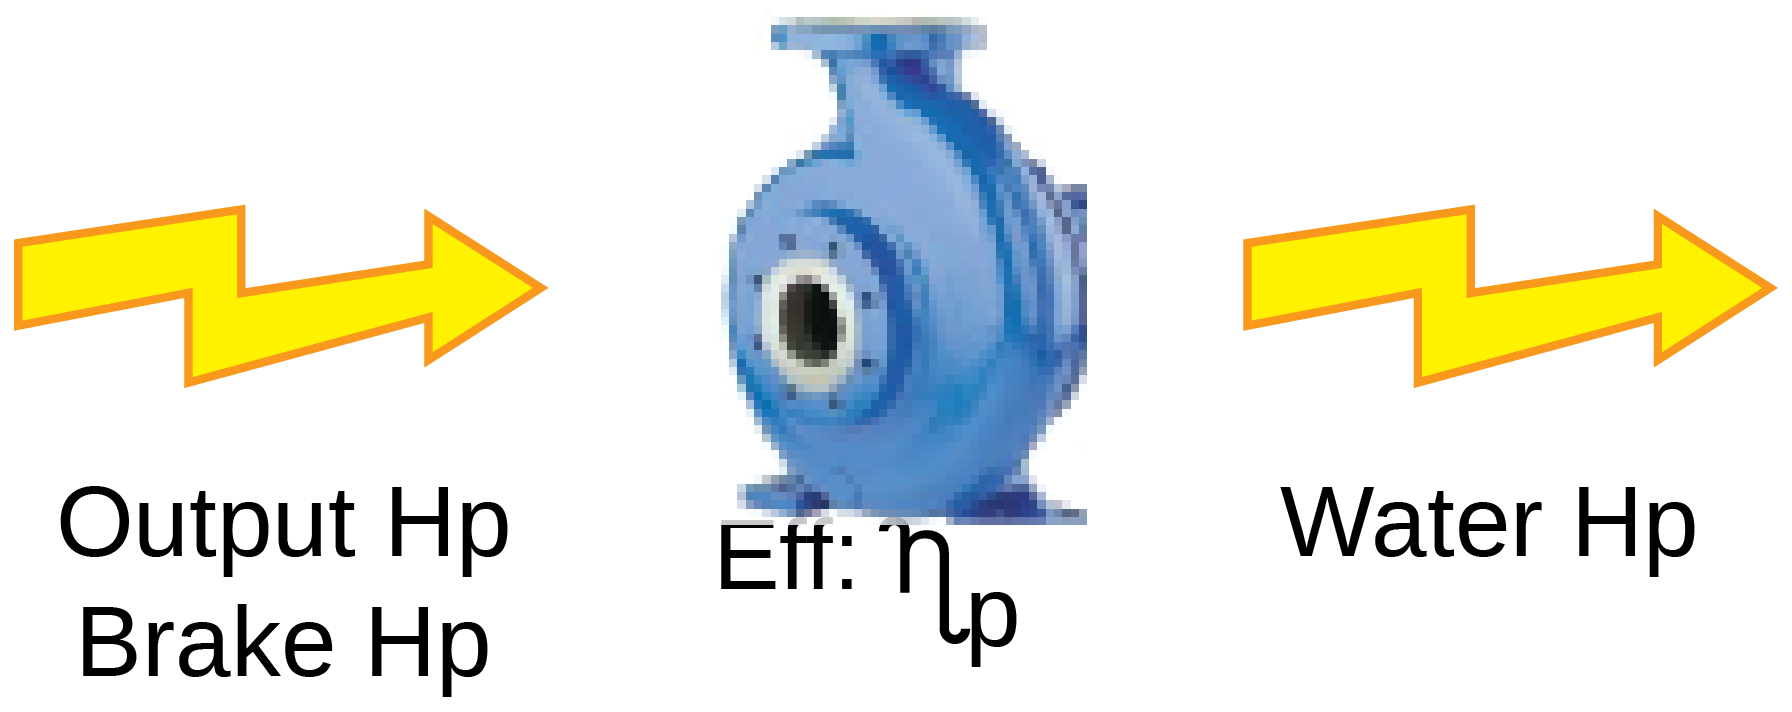
\includegraphics[scale=0.08]{PumpProblemPumpHp}\\
water Hp = flow * head\\
$400gpm*(100-5)ft*\frac{Hp}{3,960 gpm-ft}=\boxed{9.6Hp}$\\
\vspace{0.4cm}
pump efficiency - $\eta_p$=$\frac{9.6Hp}{12Hp}*100=\boxed{79\%}$
\vspace{0.4cm}

\item A flow of 200 gpm  is pumped against a total head of 4.0 feet. · The pump is 78\% efficient and the motor' is 90\% efficient. Calculate the input Hp.\\
\vspace{0.4cm}
water Hp = flow * head\\
$200GPM*4ft*\frac{Hp}{3,960 GPM-ft}=0.2Hp$\\
\vspace{0.4cm}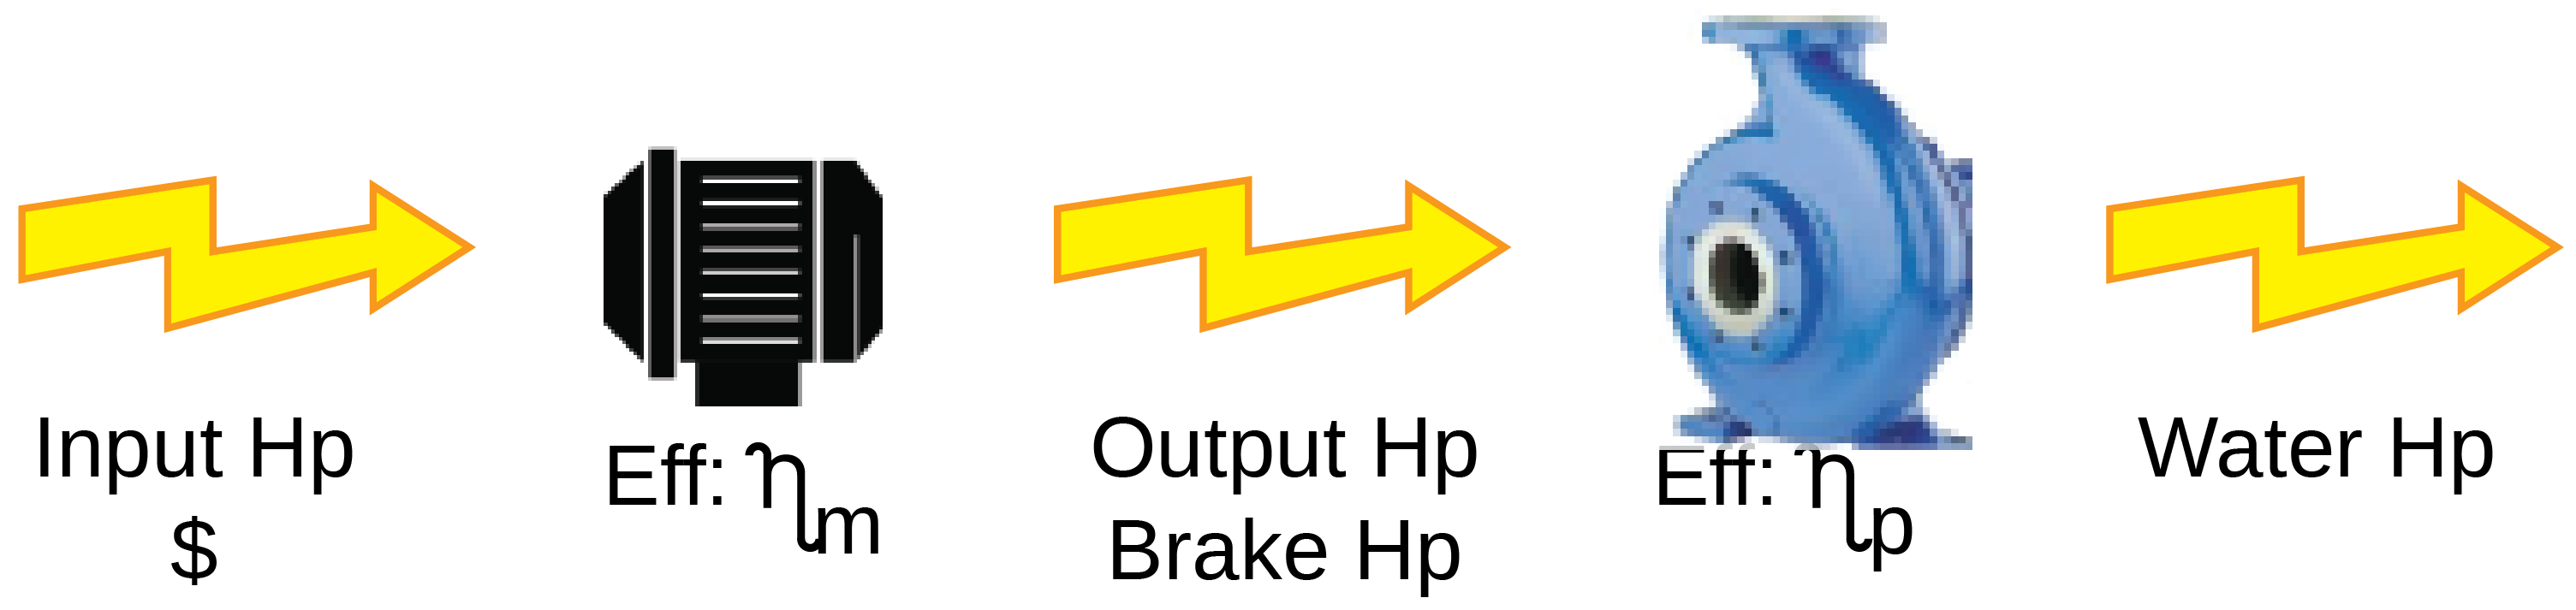
\includegraphics[scale=0.08]{PumpProblem}\\
water Hp=brake Hp*pump efficiency, and\\
brake Hp=input Hp*motor efficiency\\
Therefore, water Hp=input Hp*motor efficiency*pump efficiency\\
\vspace{0.4cm}
input Hp=$\frac{water \enspace Hp}{motor \enspace efficiency*pump \enspace efficiency}=\frac{0.2}{0.9*0.78}=\boxed{0.28Hp}$

\pagebreak

\item 500,000 gpd of secondary· effluent is pumped to  a  storage  pond  for  reuse  as golf course irrigation water.  The water is lifted 12 feet in the plant, and then pumped up another 75 feet to the storage pond. Friction losses are assumed to be 10\% of the static head.  Assuming the pump efficiency of 70\% and a motor efficiency of 92\% and an electrical cost of \$0.0725 per KWh, calculate the daily cost of pumping this water.\\
\vspace{0.4cm}
Solution:\\

water Hp = flow * head\\
\vspace{0.4cm}
$\frac{500,000gal}{day}*\frac{day}{1440min}*(87ft-static \enspace head+87*0.1ft-friction \enspace head)*\frac{Hp}{3,960 GPM-ft}$\\
$=8.39 - water \enspace Hp$\\
\vspace{0.4cm}
input Hp=$\frac{water \enspace Hp}{motor \enspace efficiency*pump \enspace efficiency}=\frac{8.39}{0.92*0.70}=\boxed{13Hp}$\\
\vspace{0.4cm}
Electrical cost=$13Hp*\frac{0.746kW}{Hp}*\frac{24hrs}{day}*\frac{\$0.0725}{kWh}=\boxed{\frac{\$16.87}{day}}$

\vspace{0.4cm}


\item A pump motor (93\% efficient) generates an output of 130 HP and runs 75\% of the time. Electricity costs an average of 8.455 cents per kilowatt-hour. What is the monthly cost of operating this pump in \$ per month?\\
\vspace{0.4cm}
$\frac{130Hp}{0.93}*\frac{0.746kW}{Hp}*\frac{24hrs}{day}*\frac{30days}{month}*0.75*\frac{\$0.08455}{kWh}=\boxed{\frac{\$4,761}{month}}$
\pagebreak


\item A wet well is 8 ft x 8 ft x 16.5 ft deep and receives a continuous flow of 310,000 gpd.  A 500 gpm pump draws down 12 feet of water each pumping cycle.  The motor that drives the pump draws 52.5 Hp when it pumps.  The cost of electricity is \$0.0755 per kilowatt - hour.  Calculate\\ 
(a) the time it takes to pump down the wet well, and\\
(b) The daily electrical energy cost for this pump.\\


\vspace{0.4cm}
Solution:\\
@$\frac{310,000gal}{day}*\frac{day}{1440min}=\frac{215.3gal}{min}$\\
\vspace{0.4cm}
Volume of wetwell that will be pumped down with the 500 gpm pump and a 215.3 gpm flow to the wetwell:\\
$\frac{500gal}{min}-\frac{215.3gal}{min}=\frac{284.7gal}{min}$\\
\vspace{0.4cm}
Minutes required to pump down the wetwell :\\
$8*8*12ft^3*\frac{7.48gal}{ft^3}*\frac{min}{284.7gal}=\boxed{20.2min}$\\
\vspace{0.4cm}
Time to fill wetwell with pump off @215.3gal/min influent flow:
\\
$8*8*12ft^3*\frac{7.48gal}{ft^3}*\frac{min}{215.3gal}=26.7min$\\
\vspace{0.4cm}
\# of cycles per day:\\
$\frac{cycle}{(20.2+26.7)min}*\frac{1440min}{day}=\frac{30.7cycles}{day}$\\
\vspace{0.4cm}
\# of hrs pump operational:\\
$\frac{20.2min}{cycle}*\frac{30.7 cycles}{day}*\frac{hrs}{60min}=\frac{10.33hours}{day}$\\
\vspace{0.4cm}
Daily electrical cost:\\
$52.5Hp*\frac{0.746kW}{Hp}*\frac{10.33hrs}{day}*\frac{\$0.0755}{kWh}=\boxed{\frac{\$30.54}{day}}$\\
\pagebreak


\item A 6-year old pump motor is to be replaced at a net cost of \$15,800. The new motor, just like the old one, would run 65\% of the time. Both existing and replacement motors would operate at 125 output Hp. The existing motor efficiency is 86\% while the replacement motor would be guaranteed at 94\% efficiency. Electricity currently averages \$0.088 per kWh.\\
(a) Calculate the energy cost savings per year (to the nearest dollar) if the existing motor is replaced with the new motor (neglect any consideration of impact upon demand charges or interest on capital).\\ (b) What is payback period to the nearest tenth of a year.
\vspace{0.4cm}
Energy cost savings per year:\\
Input Hp for old motor:$\frac{125}{0.86}=145.35Hp$\\
Input Hp for old motor:$\frac{125}{0.94}=132.98Hp$\\
Energy cost savings:\\$(145.35-132.98)Hp*\frac{0.746kW}{Hp}*\frac{(365*24*0.65)hrs}{yr}*\frac{\$0.088}{kWh}=\boxed{\frac{\$4,623.94}{yr}}$\\
\vspace{0.4cm}
Calculate payback:\\
$\$15,800*\frac{yr}{\$4,623.94}=\boxed{3.4yr}$

\item A 8 ft diameter cylindrical wetwell receives an average incoming flow if 135 gpm and is pumped down with a pump that delivers 450 gpm again a total dynamic head of 120 ft.  The pump is controlled using two floats; a stop float located at 2.5 ft and a start float located at 16 ft.  If the pump motor is rated at 88\% and the pump at 77\%, what is the monthly (30 days/month) for running this pump if power costs are \$0.11/Kwh? (Ans:  \$356/month)


\vspace{0.4cm}
Volume of wetwell that will be pumped down with the 450 gpm pump and a 135 gpm flow to the wetwell:\\
$\frac{450gal}{min}-\frac{135gal}{min}=\frac{315gal}{min}$\\
\vspace{0.4cm}
Minutes required to pump down the wetwell :\\
$0.785*8^2*(16-2.5)ft^3*\frac{7.48gal}{ft^3}*\frac{min}{315gal}=\boxed{16.1min}$\\
\vspace{0.4cm}
Time to fill wetwell with pump off @135gal/min influent flow:
\\
$[0.785*8^2*(16-2.5)]ft^3*\frac{7.48gal}{ft^3}*\frac{min}{135gal}=37.6min$\\
\vspace{0.4cm}
\# of cycles per day:\\
$\frac{cycle}{(16.1+37.6)min}*\frac{1440min}{day}=\frac{26.8cycles}{day}$\\
\vspace{0.4cm}
\# of hrs pump operational:\\
$\frac{16.1min}{cycle}*\frac{26.8 cycles}{day}*\frac{hrs}{60min}=\frac{7.19hours}{day}$\\
\vspace{0.4cm}
Daily electrical cost:\\
$\frac{450gpm*120ft}{0.88*0.77}*\frac{Hp}{3,960 gpm-ft}*\frac{0.746kW}{Hp}*\frac{7.19hrs}{day}*\frac{30days}{month}*\frac{\$0.11}{kWh}=\boxed{\frac{\$356}{day}}$\\
\vspace{1cm}


\item A pump operating at 80\% effieciency generates an water Hp of 60 HP and runs 75\% of the time. Assuming the pump motor is 90\% efficent and electricity costs an average of \$0.0821 per kilowatt-hour. The monthly (30 days) cost of operating this pump is:\\
\vspace{0.4cm}
$\frac{60Hp}{0.90*0.80}*\frac{0.746kW}{Hp}*\frac{24hrs}{day}*\frac{30days}{month}*0.75*\frac{\$0.0821}{kWh}=\boxed{\frac{\$2,756}{month}} - Correct \enspace Answer$\\
$\frac{60Hp}{0.8}*\frac{0.746kW}{Hp}*\frac{24hrs}{day}*\frac{30days}{month}*0.75*\frac{\$0.0821}{kWh}=\boxed{\frac{\$2,480}{month}}$\\
$\frac{60Hp}{0.90}*\frac{0.746kW}{Hp}*\frac{24hrs}{day}*\frac{30days}{month}*0.75*\frac{\$0.0821}{kWh}=\boxed{\frac{\$2,205}{month}}$\\
$\frac{60Hp}{0.90*0.80}*\frac{0.746kW}{Hp}*\frac{24hrs}{day}*\frac{30days}{month}*\frac{\$0.0821}{kWh}=\boxed{\frac{\$3,675}{month}}$

\item A 8 ft diameter cylindrical wetwell receives an average incoming flow if 135 gpm and is pumped down with a pump that delivers 450 gpm again a total dynamic head of 120 ft. The pump is controlled using two floats; a stop float located at 2.5 ft and a start float located at 16 ft. If the pump motor is rated at 88\% and the pump at 77\%, what is the monthly (30 days/month) for running this pump if power costs are \$0.11/Kwh? (Ans: \$356/month) 

\item  A 8 ft diameter cylindrical wetwell receives an average incoming flow if 135 gpm and is pumped down with a pump that delivers 450 gpm again a total dynamic head of 120 ft. The pump is controlled using two floats; a stop float located at 2.5 ft and a start float located at 16 ft. If the pump motor is rated at 88\% and the pump at 77\%, what is the monthly (30 days/month) for running this pump if power costs are \$0.11/Kwh? (Ans: \$356/month)


\item If a wasting pump has a fixed pump rate of 250 GPM, and your calculation
indicates you must waste 126,000 gallons, what hourly cycle rate do you set
the timer?\\
a. Turn pump on 21 minutes every day\\
b. Turn pump on 504 minutes every hour\\
c. Turn pump on 42 minutes every day\\
d. Turn pump on 21 minutes every hour\\

\vspace{0.3cm}
Solution:\\
\vspace{0.2cm}
$\frac{min}{hr}=\frac{126,000 \enspace gal}{day}*\frac{day}{24 \enspace hrs}*\frac{min}{250 \enspace gal}=\boxed{\frac{21 \enspace min}{hr}}$



\item  How long will it take to pump down 25 feet of water in a 110 ft diameter cylindrical tank when using a 1420 gpm pump. 

a. 26 hours and 56 minutes \\
*b. 26 hours and 33 minutes \\
c. 2 hours and 47 minutes \\
d. 12 hours and 36 minutes 


\item  A positive displacement pump should be started up with the discharge valve closed in order to avoid any problems with "air lock". 

a. True \\
*b. False 


\item  Brake horse power is the input power to the motor 

a. True \\
*b. False 


\item  Cost of electrical usage for pumps is based upon kilowatt per hour 

a. True \\
*b. False 


\item  A centrifugal pump can be used to pump sludge. 

*a. True \\
b. False 


\item  Variable speed sludge pumps may be used to keep the density of the sludge nearly constant. 

*a. True \\
b. False

\item The keeping of records of plant operation and maintenance, even when a portion of the plant is temporarily out of balance, is an integral part of good operation.\\
*a. True\\
b. False 


\item  A positive displacement pump could be damaged if it is started with the discharge valve closed. \\

*a. True \\
b. False 


\item  The common unit of power or rate of doing work is horsepower. This· is equal to 746 ft. lbs/min. 

*a. True \\
b. False 


\item  Total dynamic head is the sum of the suction head and the discharge head minus the friction head 

a. True \\
*b. False 


\item  Water power is the output power of the pump 

*a. True \\
b. False 


\item  A positive displacement pump should be started up with the discharge valve closed in order to avoid any problems with "air lock". 

a. True \\
*b. False 


\item  Brake horse power is the input power to the motor 

a. True \\
*b. False 


\item  Cost of electrical usage for pumps is based upon kilowatt per hour 

a. True \\
*b. False 


\item  The common unit of power or rate of doing work is horsepower. This· is equal to 746 ft. lbs/min. 

*a. True \\
b. False 


\item  Total dynamic head is the sum of the suction head and the discharge head minus the friction head 

a. True \\
*b. False 


\item  Water power is the output power of the pump 

*a. True \\
b. False 

\item  What is the vertical distance between the elevation of the free water surface at the suction and that of the free water surface at the discharge of a pump called?\\
a.	Discharge head.\\
b.	Dynamic head.\\
c.	Velocity head.\\
*d.	Static head.\\

\item If a wasting pump has a fixed pump rate of 250 GPM, and your calculation
indicates you must waste 126,000 gallons, what hourly cycle rate do you set
the timer?\\
a. Turn pump on 21 minutes every day\\
b. Turn pump on 504 minutes every hour\\
c. Turn pump on 42 minutes every day\\
*d. Turn pump on 21 minutes every hour\\

\item A positive displacement pump is connected to a 25' wide x 125' long x 12' side water depth aerobic digester. How long will it take to empty the contents of the digester if the pump rate is 225 gallons per minute?\\
a. 15.3 hours\\
b. 2.8 hours\\
*c. 20.8 hours\\
d. 15.6 hours\\

\item A centrifuge is fed sludge with a concentration of 3.4\% solids. If the sludge feed rate is set at 50 gallons per minute, what is the centrifuge loading rate
in pounds per hour?\\
a. 763 lbs/hour\\
*b. 850 lbs/hour\\
c. 735 lbs/hour\\
d. 960 lbs/hour\\

\item Calculate the surface loading rate for a treatment plant with 4 clarifiers each
with a 100 foot diameter. The plant has an influent flow of 35 MGD.\\
a. 279 gal/sq ft\\
b. 950 gal/sq ft\\
c. 4,459 gal/sq ft\\
*d. 1,115 gal/sq ft\\

\item Calculate the flow velocity in feet/minute if 7.5 MGD of flow passes through a channel that is 3' wide x 4' deep, and the depth of flow is 15 inches.\\
*a. 186 ft/min\\
b. 58 ft/min\\
c. 202 ft/min\\
d. 46.5 ft/min\\

\item Determine the pounds per day of primary solids removed at a plant with a flow rate of 1.5 MGD and the following data:\\
Clear Waters Fall 2013\\
Influent TSS = 250 mg/L\\
Primary Effluent TSS = 150 mg/L,\\
Final Effluent TSS = 12 mg/L\\
a. 1,101 lbs/day\\
*b. 1,251 lbs/day\\
c. 982 lbs/day\\
d. 2,977 lbs/day\\

\item A sewage pump is located above the wet well which is 8 feet deep and the
pump is pumping to an above ground clarifier with 12 feet depth of water.
The pump manufacturer has given you the pump characteristics curve
which shows Total Dynamic Head vs. flow rates. If the operating wet well
water depth is 6 feet, what is the total dynamic head in order to determine
pumping rate from the chart? Assume the top of the wet well and the
bottom of the clarifier are at the same elevation.\\
a. 12 feet\\
b. 20 feet\\
*c. 14 feet\\
d. 10 feet\\

\item A sewage pump is located above the 8-foot diameter wet well which is
8 feet deep and the pump is pumping to an above ground clarifier. The flow
meter on the pump is not operating and you want to calculate the pumping
rate by measuring the drop in wet well water level during when inflow to
wet well is minimal? If the drop in water level in one minute is 2 feet, what
is the approximate pumping rate in gallons per minute?\\
a. 250 GPM\\
b. 375 GPM\\
c. 500 GPM\\
*d. 750 GPM\\

\item The head against which a pump must operate:\\
a. Is the sum of the static head and the head due to friction loss.\\
b. Must always be above the shut-off head.\\
c. Is the static head.\\
d. Is the friction head.\\
\item What term describes the condition that exists when the source of the water supply is below the centerline of the pump?\\
a. Pressure head\\
b. Velocity head\\
c. Suction lift\\
d. Total discharge head\\

\item  A pump operating at 80\% efficiency generates an water Hp of 60 HP and runs 75\% of the time. Assuming the pump motor is 90\% efficent and electricity costs an average of \$0.0821 per kWh. The monthly (30 days) cost of operating this pump is:\\

*a. \$2,756 \\
b. \$2,480 \\
c. \$2,205 \\
d. \$3,675 






\end{enumerate}






\chapterimage{QuizCover} % Chapter heading image

\chapter{Constituents Properties and Analysis Assessment}
% \textbf{Multiple Choice}

\section*{Constituents Properties and Analysis Assessment}

\begin{enumerate}

\item Hazardous conditions in a manhole, wetwell or other similar type of structure may not be always be detected by the presence of odor because:\\

a. some toxic gases have no detectable odor \\
b. the environment may be oxygen deficient \\
c. some gases may deaden the sense of smelll \\
d. not all explosive gases have detectable odor \\
*e. all of the above \\

\item An operator should not enter an enclosed structure if the percentage of oxygen in the air is less than:\\

*a. 19.5\% \\
b. 23.5\% \\
c. 27.2\% \\
d. 32.5\% \\

\item Digester gas containing 60% methane by volume will likely explode when exposed to a spark or flame.\\

a. True \\
*b. False \\

\item Prior to working in a drained anaerobic digester, confined space entry permits must be prepared.\\

*a. True \\
b. False \\

\item Hydrogen sulfide gives off an odor similar to \\

a. Ammonia. \\
b. Chlorine gas \\
*c. Rotten eggs \\
d. Decayed wood. \\

\item Which of the following is not a characteristic of hydrogen sulfide? \\

a. Foul odors \\
*b. Lighter than air \\
c. Toxic \\
d. Corrosiveness \\
e. Explosiveness \\

\item If you come upon a co-worker who is not breathing, you should immediately \\

a. Apply cold compresses to the worker's forehead \\
b. Check for bleeding \\
*c. Call for help \\
d. Start CPR \\

\item What is the first, immediate, action you should take if concentrated acid is spilled on the floor? \\

a. Pour sodium nitrate and wash with warm water \\
b. Run to a shower and wash yourself thoroughly \\
*c. Sound the alarm \\
d. Wash with water and neutralize with sodium bicarbonate (baking soda) \\

\item Key steps in a safety program would not include \\

a. Controlling work habits \\
*b. Injury records for the operator \\
c. Locating hazards \\
d. Medical insurance for all employees \\

\item Three waterborne diseases are \\

a. Mumps, measles, colds \\
b. Scarlet fever, pneumonia, hay fever \\
*c. Typhoid fever, dysentery, cholera. \\
d. TB, diptheria, chickenpox \\

\item Improper handling, storing or preparing solutions of chemicals can cause \\

a. Burns \\
b. Explosions \\
c. Loss of eye sight \\
*d. All of the above \\

\item What disease is not considered to be normally conveyed or transmitted by untreated wastewater? \\

a. Amoebic dysentery \\
b. Hepatitis \\
*c. Malaria. \\
d. Chlorea. \\

\item Pathogens \\

*a. Are bacteria or virus that cause disease \\
b. Are bacteria which do not occur in water \\
c. Can obtain their food supply without help \\
d. Are not harmful to man \\

\item Employee hazards include \\

a. Noxious or toxic gases or vapors \\
b. Oxygen deficiency \\
c. Physical injuries \\
*d. All of the above \\

\item What is the proper slope of a ladder?\\
*a. Every 4 feet up the ladder is 1 foot out from the wall.\\
b.  Every 5 feet up the ladder is 1 foot out from the wall.\\
c.  Every 6 feet up the ladder is 1 foot out from the wall.\\
d.  Every 7 feet up the ladder is 1 foot out from the wall.


\item What is the safe oxygen level for entering a confined space?
a.  14 to 16 ppm.\\
b.  17 to 19 ppm.\\
*c. 20 to 22 ppm.\\
d.  23 to 25 ppm.

\item Cluttered work areas can cause accidents. Keep work areas clean. When you are finished with tools, put them:\\
a.  On the table.\\
b.  Under the table.\\
c.  On your supervisor’s desk.\\
*d. In the tool cabinet.


\item What type of tools are recommended to perform maintenance on an anaerobic digester?\\
*a. Brass.\\
b.  Stainless steel.\\
c.  Carbon steel.\\
d.  None of the above.

\item Before entering a permit-required confined space, you must:\\
a.  Check the atmosphere with a calibrated gas detector.\\
b.  Make notification that personnel are entering the space.\\
c.  Lock out and tag out all equipment.\\
*d. All of the above.


\item When working on a chemical feed pump, what of the following is not required?\\
a.  Nitrile gloves.\\
b.  Safety glasses.\\
*c. Leather work gloves.\\
d.  Full face shield.

\item When making a sulfuric acid dilution, the appropriate method is:\\
a.  Add the water to the acid.\\
*b. Add the acid to the water.\\
c.  Add both at the same time.\\
d.  None of the above.


\item When aluminum sulfate mixes with water, a very $\rule{2cm}{0.15mm}$ combination occurs.\\
a.  Noxious.
*b. Slippery.
c.  Colorful.
d.  Tacky.


\item Operators working with any form of lime are exposed to a number of hazards. Goggles, approved respiratory protection, emergency eyewash and deluge shower are necessary safety precautions. What else may be kept on hand to help flush eyes in case of severe exposure?\\
a.  Inert absorbent materials.\\
b.  A mild solution of acetic acid.\\
*c. A mild solution of boric acid.\\
d.  None of the above.

\item A mixture of 85\%-95\% atmospheric air in combination of 5\%-15\% methane creates which of the following?\\
*a. An explosive condition\\
b. Struvite\\
c. Excess pressure\\
d. Increased BTU

\item The first step the maintenance staff should take in properly locking and tagging out a piece of equipment is to $\rule{2cm}{0.15mm}$.\\
*a. Alert the operator on duty.
b.  Turn the equipment off at the motor control center (MCC).\\
c.  Pull the switch on the electrical panel to “OFF.”\\
d.  Fill out the tags.\\


\item When working in an area with two or more floor coverings, be sure that they are always $\rule{2cm}{0.15mm}$.\\
a.  Overlapping one another.\\
*b. Secured together.\\
c.  Separated from one another.\\
d.  At the entrances and exits only.

\item When manually lifting any object, be sure to $\rule{2cm}{0.15mm}$.\\
a.  Hold it at arm’s length.\\
b.  Keep your back bent and hold it low.\\
*c. Keep it close to your body and use leg strength.\\
d.  Keep your knees locked and bend at the waist.


\item Oxygen deficiency becomes a concern when the oxygen level in a confined space is less than $\rule{2cm}{0.15mm}$.\\
*a. 19.5\%.\\
b.  22.5\%.\\
c.  25.5\%.\\
d.  28.5\%.

\item Which of the following provides safety information for potentially hazardous or toxic materials?\\
a.  EPA.\\
b.  OSHA.\\
c.  CFR.\\
*d. SDS.

\item The threshold limit value concentration for chlorine vapor is $\rule{2cm}{0.15mm}$.
a.  0.1 ppm.\\
b.  0.3 ppm.\\
*c. 0.5 ppm.\\
d.  1.0 ppm.

\item When working in confined spaces where flammable gases may be present, use only tools made of $\rule{2cm}{0.15mm}$.
a.  Stainless steel.\\
b.  Lead.\\
c.  Iron.\\
*d. Beryllium.

\item Presence of hydrogen sulfide cannot always be detected by its characteristic odor \\

*a. True \\
b. False \\

\item The quantities and dosing requirements for a particular wastewater chemical can be found in the SDS \\

a. True \\
*b. False \\

\item Hydrogen sulfide in addition to creating an odor nuisance can be an explosion hazard when mixed with air in certain concentrations. \\

*a. True \\
b. False \\

\item The lower explosive limit for methane is 40\% \\

a. True \\
*b. False \\

\item What is the proper slope of a ladder?
\begin{enumerate}
\item Every 4 feet up the ladder is 1 foot out from the wall.
\item Every 5 feet up the ladder is 1 foot out from the wall.
c. Every 6 feet up the ladder is 1 foot out from the wall.
d. Every 7 feet up the ladder is 1 foot out from the wall.
\end{enumerate}

Hydrogen sulfide at 130 ppm smells most like:
\begin{enumerate}

\item Degreaser.
\item Rotten eggs.
\item Bleach.
\item Nothing.
\end{enumerate}

\item What is the safe oxygen level for entering a confined space?
\begin{enumerate}
\item 14 to 16 ppm.
\item 17 to 19 ppm.
\item 20 to 22 ppm.
\item 23 to 25 ppm.
\end{enumerate}

\item Cluttered work areas can cause accidents. Keep work areas clean. When you are finished with tools, put them:
\begin{enumerate}
\item On the table.
\item Under the table.
\item On your supervisor’s desk.
\item In the tool cabinet.
\end{enumerate}

\item What type of tools are recommended to perform maintenance on an anaerobic digester?
\begin{enumerate}
\item Brass.
\item Stainless steel.
\item Carbon steel.
\item None of the above.
\end{enumerate}

\item Before entering a permit-required confined space, you must:
\begin{enumerate}
\item Check the atmosphere with a calibrated gas detector.
\item Make notification that personnel are entering the space.
\item Lock out and tag out all equipment.
\item All of the above.
\end{enumerate}

\item When working on a chemical feed pump, what of the following is not required?
\begin{enumerate}
\item Nitrile gloves.
\item Safety glasses.
\item Leather work gloves.
\item Full face shield.
\end{enumerate}

\item When making a sulfuric acid dilution, the appropriate
method is:
\begin{enumerate}
\item Add the water to the acid.
\item Add the acid to the water.
\item Add both at the same time.
\item None of the above.
\end{enumerate}

\item When aluminum sulfate mixes with water, a very $\rule{2cm}{0.15mm}$ combination occurs.
\begin{enumerate}
\item Noxious.
\item Slippery.
\item Colorful.
\item Tacky.
\end{enumerate}

\item Operators working with any form of lime are exposed to a number of hazards. Goggles, approved respiratory protection, emergency eyewash and deluge shower are necessary safety precautions. What else may be kept on hand to help flush eyes in case of severe exposure?
\begin{enumerate}
\item Inert absorbent materials.
\item A mild solution of acetic acid.
\item A mild solution of boric acid.
\item None of the above.

\item What safety hazard is created by a polymer spill?
\begin{enumerate}
\item explosive condition 
\item fire
\item slippery surface 
\item toxic gas
\item skin burns
\end{enumerate}
\item When is it safe to enter a manhole?
\begin{enumerate}
\item after a hazardous condition has been identified
\item after ventilation equipment has been turned on
\item when wearing an SCBA and having a back-up standing by
\item when no hazardous condition exists
\end{enumerate}

\end{enumerate}








\end{enumerate}






\chapterimage{QuizCover} % Chapter heading image

\chapter{Math Assessment}
% \textbf{Multiple Choice}

\section*{Practice Problems - Fractions}
\begin{enumerate}
\item Convert 22$\dfrac{1}{4}$ into a fraction
\item Express 10ft, 6in into fraction
\item Express 10ft, 6in into decimal
\end{enumerate}

\vspace{1cm}
\section*{Practice Problems - Decimals and Powers of Ten}
\begin{enumerate}
\item Write the equivalent of 10,000,000 as a power of ten
\item Find the product of $3.4564*10^2$
\item Find the product of $534.567*10^{-2}$
\vspace{0.2cm}
\item Find the value of $\dfrac{165.93}{10^{-2}}$
\vspace{0.2cm}
\item Find the value of $0.023*10^4$
\end{enumerate}
\vspace{1cm}
Solutions:\\
\begin{enumerate}
\item $10^7$
\item 345.64
\item 5.34567
\item 16,593
\item 230
\end{enumerate}
\section*{Practice Problems - Rounding and Significant Digits}
Round the following to the nearest hundredths (the second place after the decimal).\\
A. $2.4568$\\
B. $27.2534$\\
C. $128.2111$\\
D. $364.8762$\\
E. $354.777777$\\
F. $34.666666$\\
G. $67.33333$\\
\vspace{0.25cm}
Solution:\\
A. 2.46\\
B. 27.25\\
C. 128.21\\
D. 364.88\\
E. 354.78\\
F. 34.67\\
G. 67.33\\
Round the following to the nearest tenths (the first place after the decimal).\\
A. $2.4568$\\
B. $27.2534$\\
C. $128.2111$\\
D. $364.8762$\\
E. $354.777777$\\
F. $34.666666$\\
G. $67.33333$
Solution:\\
A. 2.5\\
B. 27.3\\
C. 128.2\\
D. 364.9\\
E. 354.8\\
F. 34.7\\
G. 67.3

\vspace{0.25cm}

Round the following answers off to the most significant digit.\\

\begin{tabular}{|l|l|l|}
\hline
 & Problem & Accurate Answer \\
\hline
A. & $25.1+26.43=51.53$ &  \\
\hline
B. & $128.456-121.4=7.056$ &  \\
\hline
C. & $85-7.92432=77.07568$ &  \\
\hline
D. & $8.564+5=13.564$ &  \\
\hline
\end{tabular}

\begin{tabular}{|l|l|l|}
\hline
 & Problem & Accurate Answer \\
\hline
A. & $26.34 \times 124.34567=3,275.26495$ &  \\
\hline
B. & $23.58 \times 34.251=807.63858$ &  \\
\hline
C. & $12,453 / 13.9=895.8992805755$ &  \\
\hline
D. & $12,457.92 \times 3=37,373.76$ &  \\
\hline
\end{tabular}

\section*{Practice Problems - Averages}
\begin{enumerate}

\item Find the average of the following set of numbers:\\
$
\begin{aligned}
&0.2 \\
&0.2 \\
&0.1 \\
&0.3 \\
&0.2 \\
&0.4 \\
&0.6 \\
&0.1 \\
&0.3
\end{aligned}
$

\item The chemical used for each day during a week is given below. Based on these data, what was the average lb/day chemical used during the week?\\

\begin{tabular}{|l|l|}
\hline
Monday & 92 lb/day\\
\hline
Tuesday & 93 lb/day \\
\hline
Wednesday & 98 lb/day\\
\hline
Thursday & 93 lb/day \\
\hline
Friday & 89 lb/day\\
\hline
Saturday & 93 lb/day \\
\hline
Sunday & 97 lb/day\\
\hline
\end{tabular}

\item The average chemical use at a plant is 77 lb/day. If the chemical inventory is 2800 lbs, how many days supply is this?

\item A well pumped for 45 days. The beginning meter reading was 7,456,400 and 45 days later the same meter was 15,154,400. What was the average flow in gallons per day?

\vspace{1cm}
\end{enumerate}
\section*{Practice Problems - Percentage}
\begin{enumerate}
\item $25 \%$ of the chlorine in a 30 -gallon vat has been used. How many gallons are remaining in the vat?

\item The annual public works budget is $\$ 147,450$. If $75 \%$ of the budget should be spent by the end of September, how many dollars are to be spent? How many dollars will be remaining?

\item A 75 pound container of calcium hypochlorite has a purity of $67 \%$. What is the total weight of the calcium hypochlorite? 

\item $3 / 4$ is the same as what percentage?

\item A $2 \%$ chlorine solution is what concentration in $\mathrm{mg} / \mathrm{L}$ ?

\item A water plant produces 84,000 gallons per day. 7,560 gallons are used to backwash the filter. What percentage of water is used to backwash?

\item The average day winter demand of a community is 14,500 gallons. If the summer demand is estimated to be $72 \%$ greater than the winter, what is the estimated summer demand? Demand - When related to use, the amount of water used in a period of time. The term is in reference to the "demand" put onto the system to meet the need of customers.

\item The master meter for a system shows a monthly total of 700,000 gallons. Of the total water, 600,000 gallons were used for billing. Another 30,000 gallons were used for flushing. On top of that, 15,000 gallons were used in a fire episode and an estimated 20,000 gallons were lost to a main break that was repaired that same day. What is the total unaccounted for water loss percentage for the month?

\item Your water system takes 75 coliform tests per month. This month there were 6 positive samples. What is the percentage of samples which tested positive?
\end{enumerate}

\vspace{0.3cm}

$Time=\dfrac{Total \enspace volume \enspace to \enspace be \enspace pumped}{Pump \enspace flow \enspace rate}$

\vspace{0.3cm}
$\implies \dfrac{(0.785*110^2*25)\cancel{ft^3}*\dfrac{7.48\cancel{gal}}{\cancel{ft^3}}}{\dfrac{1420\cancel{gal}}{min}}= \boxed{1,251 \enspace min}$\\
\vspace{1cm}
\section*{Practice Problems - Ratio and Proportion}
\begin{enumerate}
\item It takes 6 gallons of chlorine solution to obtain a proper residual when the flow is 45,000 gpd. How many gallons will it take when the flow is 62,000 gpd?

\item A motor is rated at 41 amps average draw per leg at $30 \mathrm{Hp}$. What is the actual $\mathrm{Hp}$ when the draw is 36 amps? C. 

\item If it takes 2 operators $4.5$ days to clean an aeration basin, how long will it take three operators to do the same job?

\item It takes 3 hours to clean 400 feet of collection system using a sewer ball. How long will it take to clean 250 feet?

\item It takes 14 cups of $\mathrm{HTH}$ to make a $12 \%$ solution, and each cup holds 300 grams. How many cups will it take to make a $5 \%$ solution?

\item A bike travelling at 5 miles/hr completes a journey in 40 minutes. How long would the same journey take if the speed was increased to 8 miles/hr?
\end{enumerate}
\vspace{1cm}

\textbf{Solution}
\begin{enumerate}
\item The gallons chlorine and flow are directly related. 

Thus,

$\dfrac{6}{45,000}=\dfrac{X}{62,000} \implies X=\dfrac{6*62,000}{45,000}=8.3 \mathrm{gallons}$


\vspace{0.25cm}

\item The amp draw and Hp are directly related.

This

$\dfrac{30}{41}=\dfrac{X}{36} \implies X=\dfrac{30*36}{41}=26.3 \mathrm{Hp}$

\vspace{0.25cm}

\item The number of operators and the days to clean are inversely related.

Thus,

$2 * 4.5 = 3*X \implies X = \dfrac{2*4.5}{3} = 3 \mathrm{days}$



\vspace{0.25cm}

\item The hours to clean and the length of system cleaned are directly proportional.

Thus,

$\dfrac{3}{400}=\dfrac{X}{250} \implies X=\dfrac{3*250}{400}=1.9 \mathrm{hours}$

\vspace{0.25cm}

\item The cups of HTH and percentage HTH solution are directly proportional.

Thus,

$\dfrac{14}{12}=\dfrac{X}{5} \implies X=\dfrac{14*5}{12}=5.8 \mathrm{cups}$

\vspace{0.3cm}

\item The bike speed and time to complete the journey are inversely related.

Thus,

$5 * 40 = 8*X \implies X = \dfrac{5*40}{8} = 25 \mathrm{min}$

\end{enumerate}

\vspace{1cm}
\section*{Practice Problems - Area and Volume}
\begin{enumerate}

\item A 60-foot diameter tank contains 422,000 gallons of water. Calculate the height of water in the storage tank.

\item What is the volume of water in ft$^3$, of a sedimentation basin that is 22 feet long, and 15 feet wide, and filled to 10 feet?

\item What is the volume in ft$^3$ of an elevated clear well that is 17.5 feet in diameter, and filled to 14 feet?

\item What is the area of the top of a storage tank that is 75 feet in diameter?\\

\item  What is the area of a wall $175 \mathrm{ft}$. in length and $20 \mathrm{ft}$. wide?\\

\item  You are tasked with filling an area with rock near some of your equipment. 1 Bag of rock covers 250 square feet. The area that needs rock cover is 400 feet in length and 30 feet wide. How many bags do you need to purchase?\\

\item A circular clearwell is 150 feet in diameter and 40 feet tall. The Clearwell has an overflow at 35 feet. What is the maximum amount of water the clearwell can hold in Million gallons rounded to the nearest hundredth?\\


\item  A sedimentation basin is 400 feet length, 50 feet in width, and 15 feet deep. What is the volume expressed in cubic feet?\\


\item  A clearwell holds $314,000 \mathrm{ft}^{3}$ of water. It is $100 \mathrm{ft}$ in diameter. What is the height of the clearwell?\\

\item  A treatment plant operator must fill a clearwell with $10,000 \mathrm{ft}^{3}$ of water in 90 minutes. What is the rate of flow expressed in GPM?\\


\item  A water tank has a capacity of 6MG. It is currently half full. It will take 6 hours to fill. What is the flow rate of the pump?\\


\item  A clearwell with the capacity of $2.5 \mathrm{MG}$ is being filled after a maintenance period. The flow rate is 2,500 GPM. The operator begins filling at 7 AM. At what time will the clearwell be full?\\

  \item A chemical feed pump with a 6-inch bore and a 6-inch stroke pumps 60 cycles per minute. Find the pumping rate in gpm.
  
  \item Determine the flow capacity of a pump in gpm if the pump lowers the water level in a 6 -foot square wet well by 8 inches in 5 minutes.

\item How much paint will it take for a single coat of the top and sidewalls of the storage tank that is 100-feet in diameter and 30-feet tall, if one gallon of paint covers 200 square feet?\\
a. $\quad 86$ gallons\\
b. $\quad 96$ gallons\\
c. $\quad 106$ gallons\\
d. $\quad 116$ gallons\\
e. $\quad 126$ gallons

\item Under like conditions, how much more water would an 8-inch pipe carry than a 4-inch pipe?\\
a.	2 times\\
b.	3 times\\
c.	4 times\\
d.	not enough information given\\


\end{enumerate}


\textbf{Solution:}\\

\begin{enumerate}
\item Volume = Surface area * height $\implies \mathrm{height}=\dfrac{\mathrm{Volume}}{\mathrm{Surface \enspace area}}$\\
\vspace{0.2cm}

\begin{tikzpicture}
\draw (0,0) ellipse (2cm and 0.3cm);
\draw (0,-2.3) ellipse (2cm and 0.3cm);
\draw [-] (2,-2.3) -- (2,0);
\draw [<->] (-2,0) -- (2,0) node [midway, above=3mm] {\hspace{0.1cm}Diameter=60'}; 
\draw [<->] (2.5,-2.3) -- (2.5,0) node [midway, below] {\hspace{1.9cm}Height=h'};
%\draw [-] (0,-4) -- (2,-2.3);
%\draw [-] (0,-4) -- (-2,-2.3);
%\draw [-] (0,-4) -- (2,-2.3);
\draw [-] (-2,0) -- (-2,-2.3);
\draw (0,-1.2) node[text width=4cm,align=center]
  {Volume=422,000 gal};
\end{tikzpicture}\\
\vspace{0.2cm}
$\implies \mathrm{height}=\dfrac{422,000 \enspace \cancel{\mathrm{gal}}*\dfrac{\cancelto{\mathrm{ft}}{\mathrm{ft}^3}}{7.48 \enspace \cancel{\mathrm{gal}}}}{0.785*60^2 \enspace \cancel{\mathrm{ft^2}}}=\boxed{101 \enspace \mathrm{ft}}$

\end{enumerate}

\vspace{1cm}
\section*{Practice Problems - Flow and Velocity}
\begin{enumerate}

\item A rectangular channel 3 ft. wide contains water 2 ft. deep flowing at a velocity of 1.5 fps.
What is the flow rate in cfs?

\item Flow in an 8-inch pipe is 500 gpm. What is the average velocity in ft/sec? (Assume pipe is flowing full)

\item A pipeline is 18” in diameter and flowing at a velocity of 125 ft. per minute. What is the flow in gallons per minute?

\item The velocity in a pipeline is 2 ft./sec. and the flow is 3,000 gpm. What is the diameter of the pipe in inches?



\item Find the flow in a 4-inch pipe when the velocity is $1.5$ feet per second.

  \item A 42-inch diameter pipe transfers 35 cubic feet of water per second. Find the velocity in $\mathrm{ft} / \mathrm{sec}$. 
  
  \item A plastic float is dropped into a channel and is found to travel 10 feet in $4.2$ seconds. The channel is $2.4$ feet wide and $1.8$ feet deep. Calculate the flow rate of water in cfs.

  \item The flow velocity of a 6-inch diameter pipe is twice that of a 12-inch diameter pipe if both are carrying 50 gpm of water. True or false?

  \item What should the flow meter read in gpm if a 4-inch diameter main is to be flushed at a velocity of $4.6$ fps?

  \item The velocity through a channel is $4.18$ fps. If the channel is 4 feet wide by 2 feet deep by 10 feet long, what is the flow rate in gpm?

  \item What is the average flow velocity in $\mathrm{ft} / \mathrm{sec}$ for a 12-inch diameter main carrying a daily flow of $2.5 \mathrm{mgd}$ ?

\end{enumerate}



\textbf{Solution:}\\

\begin{enumerate}

\item Solution:\\
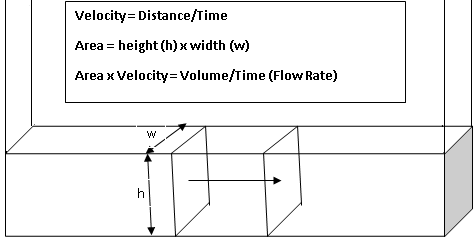
\includegraphics[scale=0.5]{ChannelFlow3}\\
$Q=V*A \implies Q = 1.5 \dfrac{ft}{sec}*(3*2)ft^2=\boxed{9\dfrac{ft^3}{sec}}$

\item Solution:\\
\vspace{0.25cm}
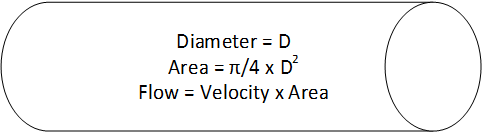
\includegraphics[scale=0.5]{PipeFlow}\\
$Q=V*A$\\
$\implies V=\dfrac{Q}{A} \implies V \Big(\dfrac{ft}{s}\Big)= \dfrac{\dfrac{500\cancel{gallon}}{\cancel{min}}*\dfrac{\cancelto{ft}{ft^3}*\dfrac{min}{60sec}}{7.48\cancel{gal}}}{0.785*\Big(\dfrac{8}{12}\Big)^2\cancelto{}{ft^2}}=\boxed{3.2ft/s}$

\item Solution:\\

\vspace{0.25cm}

The diameter of the pipe is 4 inches. Therefore, the radius is 2 inches. Convert the 2 inches to feet.
$
\begin{aligned}
&\dfrac{2}{12}=0.6667 \mathrm{ft} \\
&\mathrm{A}=\pi \times \mathrm{r}^{2} \\
&\mathrm{~A}=\pi \times(0.167 \mathrm{ft})^{2} \\
&\mathrm{~A}=\pi \times 0.028 \mathrm{ft}^{2} \\
&\mathrm{~A}=0.09 \mathrm{ft}^{2} \\
&\mathrm{Q}=\mathrm{V} \times \mathrm{A} \\
&\mathrm{Q}=1.5 \mathrm{ft} / \mathrm{sec} \times 0.09 \mathrm{ft}^{2} \\
&\mathrm{Q}=0.14 \mathrm{ft} / 3 \mathrm{sec}(\mathrm{cfs})
\end{aligned}
$



\vspace{1cm}
\end{enumerate}
\vspace{1cm}

\section*{Practice Problems - Unit Conversions}
Convert the following:\\
\begin{enumerate}
\item Convert 1000 $ft^3$ to cu. yards\\

\item Convert 10 gallons/min to $ft^3$/hr\\

\item Convert 100,000 $ft^3$ to acre-ft.\\

\item Find the flow in gpm when the total flow for the day is 65,000 gpd.

\item Find the flow in gpm when the flow is $1.3 \mathrm{cfs}$.

\item Find the flow in gpm when the flow is $0.25 \mathrm{cfs}$.

\item The flow rate through a filter is 4.25 MGD. What is this flow rate expressed as gpm?\\

\item After calibrating a chemical feed pump, you've determined that the maximum feed rate is $178 \mathrm{~mL} /$ minute. If this pump ran continuously, how many gallons will it pump in a full day?

\item A plant produces 2,000 cubic foot of water per hour. How many gallons of water is produced in an 8-hour shift?
\end{enumerate}
\textbf{Solution}
\begin{enumerate}
\item Solution:\\

$1000 \cancel{ft^3}*\dfrac{cu.yards}{27\cancel{ft^3}} = 37 cu.yards$

\item Solution:\\

\vspace{0.4cm}

$\dfrac{10 \enspace \cancel{\mathrm{gallons}}}{\cancel{\mathrm{min}}}*  \dfrac{\mathrm{ft}^3}{7.48 \cancel{\mathrm{gallons}}}  * \dfrac{60 \cancel{\mathrm{min}}}{\mathrm{hr}}   = \dfrac{80.2 \enspace \mathrm{ft}^3}{\mathrm{hr}}$

\vspace{0.4cm}


\item Solution:\\

\vspace{0.4cm}

$100,000 \cancel{ft^3} * \dfrac{acre-ft}{43,560 \cancel{ft^2-ft}} =  2.3 acre-ft$\\

\vspace{0.2cm}

\textbf{Note:} From the conversion table: acre = 43,560 $ft^2$\\
Thus, acre-ft  = 43,560 $ft^2$-ft or 43,560 $ft^3$\\

\vspace{0.4cm}

\item Solution:\\

\vspace{0.4cm}

$
\dfrac{65,000 \mathrm{gpd}}{1,440 \mathrm{~min} / \mathrm{day}}=45 \mathrm{gpm}
$

\vspace{0.4cm}

\item Solution:\\
$
1.3 \dfrac{\mathrm{cfs}}{1} \mathrm{x} \dfrac{448 \mathrm{gpm}}{1 \mathrm{cfs}}=582 \mathrm{gpm}
$

\vspace{0.4cm}

\item Solution:\\

\vspace{0.4cm}

$
0.25 \dfrac{\mathrm{cfs}}{1} \times \dfrac{448 \mathrm{gpm}}{1 \mathrm{cfs}}=112 \mathrm{gpm}
$

\vspace{0.4cm}

\item Solution:\\

\vspace{0.2cm}

$Flow rate, gpm=\dfrac{Flow \enspace rate, \enspace gpd}{1440 \enspace min/day}$\\

\vspace{0.2cm}

Note:  We are assuming that the filter operated uniformly over that 24 hour period.\\

\vspace{0.3cm}

$Flow rate, gpm=\dfrac{4.25 \enspace \dfrac{\cancel{MG}}{\cancel{day}} *1,000,000 \enspace \dfrac{gal}{\cancel{MG}}}{1440\dfrac{min}{\cancel{day}}}=\boxed{2,951 \enspace gpm}$


\item Solution:\\

\vspace{0.4cm}

$\dfrac{2000 \enspace \cancel{\mathrm{ft}^3}}{\cancel{hr}}*  \dfrac{7.48 \enspace{\mathrm{gallons}}}{\cancel{\mathrm{ft}^3}}  * \dfrac{60 \enspace \cancel{\mathrm{hr}}}{\mathrm{shift}}   = \boxed{\dfrac{119,680 \enspace \mathrm{gallons}}{\mathrm{shift}}}$

\vspace{0.4cm}
\end{enumerate}


\vspace{1cm}

\section*{Practice Problems - Concentration}
\begin{enumerate}
\item What is the concentration in mg/l of  4.5\% solution of that substance.

\item How many lbs of salt is needed to make 5 gallons of a 2,500mg/l solution

\end{enumerate}
\vspace{0.25cm}
\textbf{Solution}\\
\begin{enumerate}
\item 45,000 mg/l

\item Applying pounds formula:  lbs salt = $\dfrac{5}{1,000,000}*2,500*8.34=\boxed{0.14lbs}$
\end{enumerate}


\vspace{1cm}
\section*{Practice Problems - Density and Specific Gravity}
\begin{enumerate}

\item What is the specific gravity of a 1 ft$^3$ concrete block which weighs 145 lbs?

\item What is the specific gravity of a chlorine solution if 1 (one) gallon weighs 10.2lbs?

\item How much does each gallon of zinc orthophosphate weigh (pounds) if it has a specific gravity of 1.46?

\item How much does a 55 gallon drum of 25\% caustic soda weigh (pounds) if the specific gravity is 1.28?

\end{enumerate}

\section*{Practice Problems - Detention Time}
\begin{enumerate}
\item A flocculation basin is 7 ft deep, 15 ft wide, and 30 ft long. If the flow through the basin is 1.35 MGD, what is the detention time in minutes?

\item A tank has a diameter of 60 feet with an overflow depth at 44 feet. The current water level is 16 feet. Water is flowing into the tank at a rate of 250 gallons per minute. At this rate, how many days will it take to fill the tank to the overflow?

\item How long will it take to fill a 50 gallon hypochlorite tank if the flow is $5 \mathrm{gpm}$ ?

\item Find the detention time in a 45,000 gallon reservoir if the flow rate is $85 \mathrm{gpm}$.

\item If the fuel consumption to the boiler is 35 gallons per day. How many days will the 500 gallon tank last.

\item The sedimentation basin in a water plant contains 5,775 gallons. What is the detention time if the flow is $175 \mathrm{gpm}$.
\end{enumerate}

\textbf{Solution}\\
\begin{enumerate}
\item Solution:\\
\vspace{0.25cm}
\begin{tikzpicture}

\pgfmathsetmacro{\cubexx}{4}
\pgfmathsetmacro{\cubeyy}{1.5}
\pgfmathsetmacro{\cubezz}{2}
\pgfmathsetmacro{\cubex}{4}
\pgfmathsetmacro{\cubey}{0.5}
\pgfmathsetmacro{\cubez}{2}
\filldraw [fill=lightgray!20, draw=black] (0,-\cubey,0) -- ++(-\cubexx,0,0) -- ++(0,-\cubeyy,0) -- ++(\cubexx,0,0) -- cycle ;
\filldraw [fill=lightgray!20, draw=black] (0,-\cubey,0) -- ++(0,0,-\cubezz) -- ++(0,-\cubeyy,0) -- ++(0,0,\cubezz) -- cycle;
\filldraw [fill=lightgray!20, draw=black] (0,-\cubey,0) -- ++(0,0,-\cubezz) -- ++(0,-\cubeyy,0) -- ++(0,0,\cubezz) -- cycle;
\filldraw [fill=lightgray!20, draw=black] (0,-\cubey,0) -- ++(-\cubexx,0,0) -- ++(0,0,-\cubezz) -- ++(\cubexx,0,0) -- cycle;
%\draw (0,-0.5,0) -- ++(-\cubex,0,0) -- ++(0,-\cubey,-\cubez) -- ++(\cubex,0,0) -- cycle;
\draw (-\cubex,0,0) -- ++(0,0,-\cubez) -- ++(0,-\cubey,0) -- ++(0,0,\cubez) -- cycle;
\draw (0,-\cubey,0) -- ++(-\cubex,0,0) -- ++(0,0,-\cubez) -- ++(\cubex,0,0) -- cycle;




\filldraw [fill=white, draw=black] (0,0,0) -- ++(-\cubex,0,0) -- ++(0,-\cubey,0) -- ++(\cubex,0,0) -- cycle ;
\filldraw [fill=white, draw=black] (0,0,0) -- ++(0,0,-\cubez) -- ++(0,-\cubey,0) -- ++(0,0,\cubez) -- cycle;
\filldraw [fill=white, draw=black] (0,0,0) -- ++(0,0,-\cubez) -- ++(0,-\cubey,0) -- ++(0,0,\cubez) -- cycle;
\filldraw [fill=white, draw=black] (0,0,0) -- ++(-\cubex,0,0) -- ++(0,0,-\cubez) -- ++(\cubex,0,0) -- cycle;
%\draw (0,-0.5,0) -- ++(-\cubex,0,0) -- ++(0,0,-\cubez) -- ++(\cubex,0,0) -- cycle;
%\filldraw [fill=white, draw=black] (-\cubex,0,0) -- ++(0,0,-\cubez) -- ++(0,-\cubey,0) -- ++(0,0,\cubez) -- cycle;
%\filldraw [fill=white, draw=black] (0,-\cubey,0) -- ++(-\cubex,0,0) -- ++(0,0,-\cubez) -- ++(\cubex,0,0) -- cycle;

\draw [<->] (-4,-2.3) -- (0,-2.3) node [midway, below] {\scriptsize{30' long}};
\draw [<->] (1,-1.3) -- (1,.2) node [midway, below] {\hspace{2.2cm}\scriptsize{7' deep}};
%\draw [<->] (1,.8) -- (1,.2) node [midway, below] {\hspace{2.2cm}Text Y Axis};
\draw [<->] (1,-1.3) -- (0,-2.3) node [midway, below] {\hspace{1.7cm}\scriptsize{15' wide}};
\draw [->](-6,-1) -- (-4,-1) node [midway, above] {\hspace{0.5cm}\scriptsize{1.5 MGD}};
\draw [->](0.3,-1) -- (0.9,-1) node [midway, above] {};
\end{tikzpicture}\\

\vspace{0.4cm}
$
\mathrm{DT}=\dfrac{(30*15*7) \mathrm{ft^3}*7.48\dfrac{gal}{ft^3}}{1,350,000 \dfrac{\mathrm{gal}}{day}*\dfrac{\mathrm{day}}{1440\mathrm{min}}}=25 \mathrm{min}
$


\vspace{0.4cm}


\item Solution:\\

\vspace{0.4cm}
\begin{tikzpicture}[scale=1]
\node [draw, cylinder, cylinder uses custom fill, cylinder body fill=green!20, 
cylinder end fill=green!20, shape aspect=4, rotate=90, minimum width=3cm] (c1) at 
(0,1.8){};

\coordinate(dhtop) at ($(c1.after top)!-1*.1!(c1.before top)$);
\coordinate(dhbot) at ($(c1.before bottom)!-1*.1!(c1.after bottom)$);
\coordinate(dhlabel) at ($(dhtop)!.5!(dhbot)$);
%\draw[|-|] (dhbot)--(dhtop);
%\path (dhlabel) node[right, outer sep = 2pt] {$44'$};

\node [draw, cylinder, cylinder body fill=black!20, cylinder end fill=red!20, shape aspect=4, rotate=90, minimum height=4cm, minimum width=3cm] (c) {};

\coordinate(htop) at ($(c.before top)!-1*.1!(c.after top)$);
\coordinate(hbot) at ($(c.after bottom)!-1*.1!(c.before bottom)$);
\coordinate(hlabel) at ($(htop)!.5!(hbot)+(c.north)!.9!(c.center)$);

%\draw[|-|] (hbot)--(htop);
%\path (hlabel) node[left] {}; %Modify height label here


%\node [draw, cylinder, cylinder uses custom fill, cylinder body fill=black!20, 
%cylinder end fill=lightgray!20, shape aspect=4, rotate=90, minimum width=3cm] (c1) at 
%(0,3.8){};


\node [draw, cylinder, cylinder uses custom fill, cylinder body fill=black!20, 
cylinder end fill=lightgray!20, shape aspect=4, rotate=90, minimum width=3cm] (c1) at 
(0,-1.2){};

%\node [draw, cylinder, cylinder uses custom fill, cylinder body fill=blue!20, 
cylinder end fill=green!20, shape aspect=4, rotate=90, minimum width=3cm] (c1) at 
(0,0){};

%\coordinate (center) at ($(c.before top)!0.5!(c.after top)$);
%\filldraw (center) circle (1pt);
%
%\coordinate (rlabel) at ($(center) !0.5!(c.after top)$);
%\coordinate (rtop) at ($(center)!-1*.1!(c.after top)$);

%\coordinate (rend) at ($(c.mid east)!0.5!(c.after top)$);
%\draw[-, shorten >=-10] (center) -- (rend);
%\path (rend) node[outer sep = 5pt, left] {$r$};
\draw [<->] (-1.5,2.4) -- (1.5,2.4) node [midway, above=1mm] {\hspace{0.05cm}\scriptsize{Diameter=60'}};
%\draw [<->] (1.8,2.4) -- (1.8,1.9) node [midway, midway] {\hspace{2.4cm}\scriptsize{16' Freeboard}};
%\draw [<->] (1.8,1.9) -- (1.8,-0.7) node [midway, midway] {\hspace{2.4cm}\scriptsize{28' Fill}};
%\draw [<->] (1.8,-1.1) -- (1.8,-0.7) node [midway, midway] {\hspace{2.8cm}\scriptsize{16' Current Level}};
\draw (3.3,1.9) node{\scriptsize{Overflow level = 44'}};
\draw (3.22,-0.6) node{\scriptsize{Current level = 16'}};
\draw [<-] (1.5,-0.6) -- (2.2,-0.6);
\draw [<-] (1.5,1.9) -- (2.2,1.9);
\draw[thick,->](0,3.5)--(0,2.5) node [at start, above, black] (n){\scriptsize{250 gpm}};
\end{tikzpicture}

$\mathrm{Fill \enspace time}=\dfrac{Volume}{Flow}=\dfrac{0.785*60^2*(44-16)ft^3*\dfrac{7.48 gallons}{ft^3}}{250 \dfrac{gallons}{min}*\dfrac{1440 \enspace min}{day}}=1.6 \enspace days$
\vspace{0.4cm}

\item Solution:\\

\vspace{0.4cm}

$
\mathrm{DT}=\dfrac{50 \mathrm{gal}}{5 \mathrm{gal} / \mathrm{min}}=10 \mathrm{~min}
$

\vspace{0.4cm}

\item Solution:\\

\vspace{0.4cm}

$
\mathrm{DT}=\dfrac{45,000 \mathrm{gal}}{85 \mathrm{gal} / \mathrm{min}}=529 \mathrm{~min} \quad \text { or } \dfrac{529 \mathrm{~min}}{60 \mathrm{~min} / \mathrm{hr}}=8.8 \mathrm{hrs}
$
\vspace{0.4cm}

\item Solution:\\

\vspace{0.4cm}

$
\mathrm{DT}=\dfrac{500 \text { gal }}{35 \mathrm{gal} / \text { day }}=14.3 \text { days }
$
\vspace{0.4cm}

\item Solution:\\

\vspace{0.4cm}

$
\mathrm{DT}=\dfrac{5,775 \mathrm{gal}}{175 \mathrm{gal} / \mathrm{min}}=33 \mathrm{~min}
$

\end{enumerate}
\vspace{1cm}

\section*{Practice Problems - Pounds Formula}
\begin{enumerate}

\item A water treatment plant operates at the rate of 75 gallons per minute. They dose soda ash at
14 mg/l. How many pounds of soda ash will they use in a day?

\item A water treatment plant is producing 1.5 million gallons per day of potable water, and
uses 38 pounds of soda ash for pH adjustment. What is the dose of soda ash at that plant?

\item A water treatment plant produces 150,000 gallons of water every day. It uses an
average of 2 pounds of permanganate for iron and manganese removal. What is the dose of the
permanganate? 

\item A water treatment plant uses 8 pounds of chlorine daily and the dose is 17 mg/l. How
many gallons are they producing?

\item An operator mixes 40 lb of lime in a 100-gal tank containing 80 gal of water. What is the percent of lime in the slurry?

\item A treatment plant has a maximum output of $30 \mathrm{MGD}$ and doses ferric chloride at 75 $\mathrm{mg} / \mathrm{L}$. How many pounds of Ferric Chloride does the plant use in a day?\\

\item  A treatment plant uses 750 pounds of alum a day as it treats $15 \mathrm{MGD}$. What was the dose rate?\\


\item  A treatment plant operates at 1,500 gallons a minute and uses 500 pounds of alum a day. What is the alum dose?\\

\end{enumerate}

\textbf{Solution:}
\begin{enumerate}[1.]
\item Solution:\\

\begin{figure}[h]
\begin{tikzpicture}
    \newcommand{\R}{1.5}

\path[help lines,step=.2] (0,0) grid (16,3);
\path[help lines,line width=.6pt,step=1] (0,0) grid (16,3);
%\foreach \x in {0,1,2,3,4,5,6,7,8,9,10,11,12,13,14,15,16}
%\node[anchor=north] at (\x,0) {\x};
%\foreach \y in {0,1,2,3,4,5,6}
%\node[anchor=east] at (0,\y) {\y};
%-------------CIRCLE-----------------------------------
\draw[black,fill=gray!10] (8,3) circle (\R);
\draw[black, very thick, rotate=0](6.5,3) -- (9.5,3);
\draw (8,3.6) node[text width=3cm,align=center]
  {\scriptsize{lbs/day}};
\draw (7.1,2.5) node[text width=3cm,align=center]
  {\tiny{14 mg/l}};
\draw (8.9,2.5) node[text width=3cm,align=center]
  {\tiny{75 GPM}};
  \draw (8,2)node[text width=3cm,align=center]
  {\tiny{8.34}};
\draw[black, very thick, rotate=0](7.2,1.7) -- (8,3);
\draw[black, very thick, rotate=0](8.8,1.7) -- (8,3);
\end{tikzpicture}
\end{figure}
$\dfrac{\mathrm{lbs}}{\mathrm{day}}=\mathrm{Flow}\dfrac{{\mathrm{MG}}}{\mathrm{day}}* \mathrm{Concentration}\dfrac{\mathrm{mg}}{\mathrm{l}}*8.34$
\\
\vspace{0.2cm}
$\dfrac{\mathrm{lbs}}{\mathrm{day}}=75 \dfrac{\cancel{\mathrm{gallons}}}{\cancel{\mathrm{min}}}* 1440\dfrac{\cancel{\mathrm{min}}}{\mathrm{day}}*\dfrac{\mathrm{MG}}{1,000,000 \enspace \cancel{\mathrm{gallons}}}*250\dfrac{\mathrm{mg}}{\mathrm{l}}*8.34 = \boxed{225\dfrac{lbs}{day}}$
\vspace{0.2cm}
 \item Solution:\\
 \begin{figure}[h!]
\begin{tikzpicture}
    \newcommand{\R}{1.5}

\path[help lines,step=.2] (0,0) grid (16,3);
\path[help lines,line width=.6pt,step=1] (0,0) grid (16,3);
%\foreach \x in {0,1,2,3,4,5,6,7,8,9,10,11,12,13,14,15,16}
%\node[anchor=north] at (\x,0) {\x};
%\foreach \y in {0,1,2,3,4,5,6}
%\node[anchor=east] at (0,\y) {\y};
%-------------CIRCLE-----------------------------------
\draw[black,fill=gray!10] (8,3) circle (\R);
\draw[black, very thick, rotate=0](6.5,3) -- (9.5,3);
\draw (8,3.6) node[text width=3cm,align=center]
  {\scriptsize{38 lbs/day}};
\draw (7.1,2.5) node[text width=3cm,align=center]
  {\tiny{? mg/l}};
\draw (8.9,2.5) node[text width=3cm,align=center]
  {\tiny{1.5 MGD}};
  \draw (8,2)node[text width=3cm,align=center]
  {\tiny{8.34}};
\draw[black, very thick, rotate=0](7.2,1.7) -- (8,3);
\draw[black, very thick, rotate=0](8.8,1.7) -- (8,3);
\end{tikzpicture}
\end{figure}
$\dfrac{\mathrm{lbs}}{\mathrm{day}}=\mathrm{Flow}\dfrac{{\mathrm{MG}}}{\mathrm{day}}* \mathrm{Concentration}\dfrac{\mathrm{mg}}{\mathrm{l}}*8.34 \hspace{0.2cm} \implies \mathrm{Concentration}\dfrac{\mathrm{mg}}{\mathrm{l}}=\dfrac{ \dfrac{\mathrm{lbs}}{\mathrm{day}}}{\mathrm{Flow}\dfrac{{\mathrm{MG}}}{\mathrm{day}}*8.34}$
\vspace{0.2cm}
$\mathrm{Concentration}\dfrac{\mathrm{mg}}{\mathrm{l}}=\dfrac{ 38\dfrac{\mathrm{lbs}}{\mathrm{day}}}{1.5\dfrac{{\mathrm{MG}}}{\mathrm{day}}*8.34}=\boxed{3\dfrac{\mathrm{mg}}{\mathrm{l}}}$
\\
\vspace{0.2cm}



 \item Solution:\\
 \begin{figure}[h!]
\begin{tikzpicture}
    \newcommand{\R}{1.5}

\path[help lines,step=.2] (0,0) grid (16,3);
\path[help lines,line width=.6pt,step=1] (0,0) grid (16,3);
%\foreach \x in {0,1,2,3,4,5,6,7,8,9,10,11,12,13,14,15,16}
%\node[anchor=north] at (\x,0) {\x};
%\foreach \y in {0,1,2,3,4,5,6}
%\node[anchor=east] at (0,\y) {\y};
%-------------CIRCLE-----------------------------------
\draw[black,fill=gray!10] (8,3) circle (\R);
\draw[black, very thick, rotate=0](6.5,3) -- (9.5,3);
\draw (8,3.6) node[text width=3cm,align=center]
  {\scriptsize{38 lbs/day}};
\draw (7.1,2.5) node[text width=3cm,align=center]
  {\tiny{? mg/l}};
\draw (8.9,2.5) node[text width=3cm,align=center]
  {\tiny{1.5 MGD}};
  \draw (8,2)node[text width=3cm,align=center]
  {\tiny{8.34}};
\draw[black, very thick, rotate=0](7.2,1.7) -- (8,3);
\draw[black, very thick, rotate=0](8.8,1.7) -- (8,3);
\end{tikzpicture}
\end{figure}
$\dfrac{\mathrm{lbs}}{\mathrm{day}}=\mathrm{Flow}\dfrac{{\mathrm{MG}}}{\mathrm{day}}* \mathrm{Concentration}\dfrac{\mathrm{mg}}{\mathrm{l}}*8.34 \hspace{0.2cm} \implies \mathrm{Concentration}\dfrac{\mathrm{mg}}{\mathrm{l}}=\dfrac{ \dfrac{\mathrm{lbs}}{\mathrm{day}}}{\mathrm{Flow}\dfrac{{\mathrm{MG}}}{\mathrm{day}}*8.34}$
\vspace{0.2cm}
$\mathrm{Concentration}\dfrac{\mathrm{mg}}{\mathrm{l}}=
\dfrac{ 2\dfrac{\mathrm{lbs}}{\mathrm{day}}}
{\Bigg(150,000 \dfrac{\cancel{\mathrm{Gallons}}}
{\mathrm{day}}*
\dfrac{\mathrm{MG}}
{1,000,000 \cancel{\enspace \mathrm{Gallons}}}*8.34\Bigg)}
=\boxed{3\dfrac{\mathrm{mg}}{\mathrm{l}}}$
\\
\vspace{0.2cm}


 \item Solution:\\
 \begin{figure}[h!]
\begin{tikzpicture}
    \newcommand{\R}{1.5}

\path[help lines,step=.2] (0,0) grid (16,3);
\path[help lines,line width=.6pt,step=1] (0,0) grid (16,3);
%\foreach \x in {0,1,2,3,4,5,6,7,8,9,10,11,12,13,14,15,16}
%\node[anchor=north] at (\x,0) {\x};
%\foreach \y in {0,1,2,3,4,5,6}
%\node[anchor=east] at (0,\y) {\y};
%-------------CIRCLE-----------------------------------
\draw[black,fill=gray!10] (8,3) circle (\R);
\draw[black, very thick, rotate=0](6.5,3) -- (9.5,3);
\draw (8,3.6) node[text width=3cm,align=center]
  {\scriptsize{8 lbs/day}};
\draw (7.1,2.5) node[text width=3cm,align=center]
  {\tiny{17 mg/l}};
\draw (8.9,2.5) node[text width=3cm,align=center]
  {\tiny{? MGD}};
  \draw (8,2)node[text width=3cm,align=center]
  {\tiny{8.34}};
\draw[black, very thick, rotate=0](7.2,1.7) -- (8,3);
\draw[black, very thick, rotate=0](8.8,1.7) -- (8,3);
\end{tikzpicture}
\end{figure}
$\dfrac{\mathrm{lbs}}{\mathrm{day}}=\mathrm{Flow}\dfrac{{\mathrm{MG}}}{\mathrm{day}}* \mathrm{Concentration}\dfrac{\mathrm{mg}}{\mathrm{l}}*8.34 \hspace{0.2cm}$\\
\vspace{0.2cm}
$\implies \mathrm{Flow}\dfrac{{\mathrm{MG}}}{day}=\dfrac{ \dfrac{\mathrm{lbs}}{\mathrm{day}}}{\mathrm{Concentration}\dfrac{\mathrm{mg}}{\mathrm{l}}*8.34}=\dfrac{8 \dfrac{\mathrm{lbs}}{\mathrm{day}}}{17\dfrac{\mathrm{mg}}{\mathrm{l}}*8.34}=0.056425\dfrac{{\mathrm{MG}}}{day}$\\
\vspace{0.2cm}
$0.056425\dfrac{{\mathrm{MG}}}{day}*\dfrac{1,000,000 \enspace \mathrm{Gallons}}{\mathrm{MG}}=\boxed{56,425 \enspace \mathrm{Gallons}}$
\vspace{0.2cm}


 \item Solution:\\
 \begin{figure}[h!]
\begin{tikzpicture}
    \newcommand{\R}{1.5}

\path[help lines,step=.2] (0,0) grid (16,3);
\path[help lines,line width=.6pt,step=1] (0,0) grid (16,3);
%\foreach \x in {0,1,2,3,4,5,6,7,8,9,10,11,12,13,14,15,16}
%\node[anchor=north] at (\x,0) {\x};
%\foreach \y in {0,1,2,3,4,5,6}
%\node[anchor=east] at (0,\y) {\y};
%-------------CIRCLE-----------------------------------
\draw[black,fill=gray!10] (8,3) circle (\R);
\draw[black, very thick, rotate=0](6.5,3) -- (9.5,3);
\draw (8,3.6) node[text width=3cm,align=center]
  {\scriptsize{38 lbs/day}};
\draw (7.1,2.5) node[text width=3cm,align=center]
  {\tiny{? mg/l}};
\draw (8.9,2.5) node[text width=3cm,align=center]
  {\tiny{1.5 MGD}};
  \draw (8,2)node[text width=3cm,align=center]
  {\tiny{8.34}};
\draw[black, very thick, rotate=0](7.2,1.7) -- (8,3);
\draw[black, very thick, rotate=0](8.8,1.7) -- (8,3);
\end{tikzpicture}
\end{figure}
$\mathrm{lbs}=\mathrm{Volume}{\mathrm{(MG)}}* \mathrm{Concentration}\dfrac{\mathrm{mg}}{\mathrm{l}}*8.34 \hspace{0.2cm}$\\
\vspace{0.2cm}
$ \implies \mathrm{Concentration}\dfrac{\mathrm{mg}}{\mathrm{l}}=\dfrac{ \mathrm{lbs}}{\mathrm{Volume}\mathrm{(MG)}*8.34}=\dfrac{40 \enspace \mathrm{lbs}}{80 \enspace\mathrm{gallons}*\dfrac{\mathrm{MG}}{1,000,000 \enspace \cancel{\mathrm{gallons}}}*8.34}$
\vspace{0.2cm}

\vspace{0.2cm}


\end{enumerate}

%\mathrm{Concentration}\dfrac{\mathrm{mg}}{\mathrm{l}}
\vspace{1cm}
\section*{Practice Problems - Temperature Conversion}
\begin{enumerate}
\item Convert 22\degree{C} into degree Fahrenheit.
\item Convert 56\degree{C} into degree Celsius.
\end{enumerate}
\vspace{1cm}

\section*{Preliminary Treatment} \index{Preliminary Treatment}
\begin{enumerate}
\item On an average a 12.5 yd. load of grit is hauled to the landfill once every 20 days. Plant flow averages 12.5 MGD. Calculate the rate of grit collection in ft3/MG. \\

Correct Answer(s):\\
a. 1.4

\vspace{0.4cm}
\item A grit channel is 2 feet 4 inches wide. When wastewater is flowing 8 inches deep in this channel, the velocity is found to be 1.6 ft per second. Calculate flow in MGD. \\

a. 1.55 MGD \\
*b. 1.60 MGD \\
c. 1.90 MGD \\
d. 2.50 MGD 

\vspace{0.4cm}
\item A grit channel is 2 feet 4 inches wide. When wastewater is flowing 8 inches deep in this channel, the velocity is found to be 1.6 ft per second. Calculate flow in MGD. \\

a. 1.55 MGD \\
*b. 1.60 MGD \\
c. 1.90 MGD \\
d. 2.50 MGD 



\vspace{0.4cm}
\item At a wastewater treatment plant which receives a flow rate of 650,000 gallons per day, a total of 50 cubic feet of grit was removed for the month. Calculate the rate of grit removal assuming 30 days in a month.\\
Solution:\\
$Grit Removal\frac{ft^3}{MG}=50\frac{ft^3}{ \cancel{month}}*\frac{\cancel{month}}{30\cancel{days}}*\frac{\cancel{day}}{650,000\cancel{gal}}*1,000,000\frac{\cancel{gal}}{MG}=\boxed{2.6\frac{ft^3}{MG}}$

\vspace{0.4cm}
\item On an average a 12.5 yd. load of grit is hauled to the landfill once every 20 days. Plant flow averages 12.5 MGD. Calculate the rate of grit collection in ft$^3$/MG.\\
Solution:\\
$Grit Removal\Big(\frac{ft^3}{MG}\Big)=\frac{12.5\cancel{yd^3}}{ 20\cancel{days}}*\frac{27ft^3}{ \cancel{yd^3}}*\frac{\cancel{day}}{12.5MG}=\boxed{1.4\frac{ft^3}{MG}}$

\vspace{0.4cm}
\item On an average, 2 inches of grit is collected and removed every day in a 2.2 feet wide, 205 feet long grit channel.  Knowing the average flow through that grit channel is 10 MGD calculate the rate of grit collection in ft$^3$/MG\\
Solution:\\
Grit volume accumulated:  $\frac{2}{12}ft*(2.2*205)ft^2=\frac{75.16ft^3}{day}$
Grit Collection: $\frac{\frac{75.16ft^3}{\cancel{day}}}{\frac{10MG}{\cancel{day}}}=\boxed{7.5\frac{ft^3}{MG}}$ 

\vspace{0.4cm}
\item What is the grit production rate (cu. ft/MG) if 46 cu. ft of grit is removed every five days and the daily plant flow averages 2 MGD.\\

a. 12 cu. ft/MG \\
b. 23 cu. ft/MG \\
*c. 4.6 cu. ft/MG \\
d. 9.2 cu. ft/MG\\

Solution:\\
$Grit \enspace Production \enspace Rate\Big(\frac{ft^3}{MG}\Big)=\frac{46\cancel{ft^3}}{ 5\cancel{\enspace days}}*\frac{\cancel{day}}{2MG}=\boxed{4.6\frac{ft^3}{MG}}$


\vspace{0.4cm}
\item A grit chamber is 2 feet 4 inches wide. When wastewater is flowing 8 inches deep in this channel, the flow velocity is found to be 1.6 ft per second. Calculate flow in MGD.\\


Solution:\\
\vspace{0.3cm}
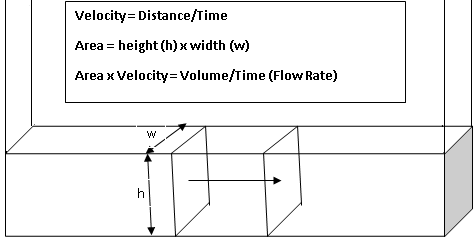
\includegraphics[scale=0.5]{ChannelFlow3}\\
$Q=V*A$\\
$Q=1.6\dfrac{ft}{s}*\Big(\dfrac{28}{12}*\dfrac{8}{12}\Big)ft^2=2.49\dfrac{ft^3}{s}$\\
$Q=2.49\dfrac{\cancel{ft^3}}{\cancel{s}}*\dfrac{(1440*60)\cancel{s}}{day}*7.48\dfrac{\cancel{gal}}{\cancel{ft^3}}\dfrac{MG}{\cancel{gal}}=\boxed{1.61MGD}$

\vspace{0.4cm}
\vspace{0.4cm}
\item  A steel bin is used to collect the daily accumulation of grit for disposal in a land fill. The bin is 8 ft long, 5.25 ft. wide, and 6 feet deep. When the bin is three-quarters full it is hauled away. This occurs on the average every 10 days. Average flow to the plant is \\3.75 MGD. What is the rate of grit collection in units of cubic feet per MG of flow?\\

Correct Answer(s):\\
a. 4.9


\vspace{0.4cm}
\item  A flow controlled grit chamber has two channels which are each 2.5 feet wide, and 20 feet long. Only one of these channels is currently in service and it receiving a flow of 4.5 MGD. The wastewater is flowing 1.5 feet deep in this channel. Calculate the velocity of this \\flow. Should we put the other channel in service?\\

Correct Answer(s): 

\vspace{0.4cm}
\item Calculate the flow, in gpd, that would pass through a grit chamber 2 feet wide, at a depth of 6 inches, with a velocity of 1 ft /sec.\\

Correct Answer(s):\\
a. 646272.0
\end{enumerate}



\section*{Primary Treatment} \index{Primary Treatment}
\begin{enumerate}
\item A clarifier has a TSS removal efficiency of 50\%.  If the influent TSS concentration is 220 mg/l, how many lbs/day of TSS are removed if the flow is 10 MGD.  Also, how many cu. ft of sludge is pumped if the sludge has a TS concentration of 5\%.\\
$lbs \enspace solids \enspace removed=(220*0.50)mg/l*10MGD*8.34=9,174lbs \enspace solids \enspace per \enspace day$
$$\frac{ft^3\enspace sludge}{day}= \frac{9,174 \enspace \cancel{lbs \enspace solids}}{day} * \frac{1 \enspace \cancel{lb \enspace sludge}}{0.05\enspace \cancel{lbs \enspace solids}}*\frac{\cancel{gal \enspace sludge}}{8.34\cancel{lb \enspace sludge}}*\frac{ft^3 \enspace sludge}{7.48 \enspace \cancel{gal}}=\boxed{2,941\frac{ft^3 \enspace sludge}{day}} $$

\item A community has a total flow of 15 MGD which is passed through a primary treatment plant which removes 60\% of the TSS and 35\% of the BOD. The average strength of the influent is 400 mg/l TSS and 275 mg/l BOD. If the total solids of the raw sludge is 5\%, how many cu. ft of sludge is pumped daily?
$lbs \enspace solids \enspace removed=(400*0.60)mg/l*15MGD*8.34=30,024lbs \enspace solids \enspace per \enspace day$
$$\frac{ft^3\enspace sludge}{day}= \frac{30,924 \enspace \cancel{lbs \enspace solids}}{day} * \frac{1 \enspace \cancel{lb \enspace sludge}}{0.05\enspace \cancel{lbs \enspace solids}}*\frac{\cancel{gal \enspace sludge}}{8.34\cancel{lb \enspace sludge}}*\frac{ft^3 \enspace sludge}{7.48 \enspace \cancel{gal}}=\boxed{9,626\frac{ft^3 \enspace sludge}{day}} $$

\item How many lbs of solids are removed daily by a primary clarifier treating a 6 MGD flow if the average influent TSS concentration is 300 mg/l and the clarifier TSS removal efficiency is 67\%?\\
As the removal efficiency is 67\%, 0.67 * 300 mg/l = 201 mg/l solids are removed.\\
The total lbs removed can be calculated using the lbs formula.\\
$ \frac{lbs \enspace solids}{day}= 6 MGD* 201  \frac{mg \enspace  SS}{l}*8.34=\boxed{10,058 \frac{lbs \enspace solids}{day}}$

\item Calculate the primary clarifier influent solids concentration if its outlet concentration is 60 mg/l and the known clarifier removal efficiency is 75\%?\\
$\frac{Actual \enspace  inlet \enspace (X)}{Actual \enspace outlet}=\frac{100}{100-Removal \enspace efficiency}$\\ 
$\frac{Actual \enspace  inlet \enspace (X)}{60}=\frac{100}{100-75}=4$\\
$\implies Actual \enspace inlet \enspace (X)=4*60 = \boxed{240 mg/l}$\\

\item A circular clarifier receives a flow of 11 MGD.  If the clarifier is 90 ft. in diameter and is 12 ft. deep, what is: a) the hydraulic/surface loading rate, b) weir overflow rate, and c) clarifier detention time in hours?\\
Solution:\\
a) Hydraulic/surface loading rate:\\
$Clarifier \enspace hydraulic \enspace loading \enspace 	\Big(\frac{gpd}{ft^2}\Big) ==\frac{\frac{11\cancel{MG}}{{day}}*\frac{10^6gal}{\cancel{MG}}}{0.785*90^2 ft^2}=\boxed{1,730gpd/ft^2}$\\
b) Weir overflow rate:\\ 
$Weir \enspace overflow \enspace rate \Big(\frac{gpd}{ft}\Big) =\frac{\frac{11\cancel{MG}}{{day}}*\frac{10^6gal}{\cancel{MG}}}{3.14*90 ft}=\boxed{38,924gpd/ft}$\\
c) Clarifier detention time:\\
$Clarifier \enspace detention \enspace time \enspace (hr) = 	\frac{ Clarifier \enspace volume (cu.ft \enspace or \enspace gal)}{Influent \enspace flow \enspace (cu.ft \enspace or \enspace gal)/hr)}$\\
$Clarifier \enspace detention \enspace time \enspace (hr) = 	\frac{(0.785*90^2*15)\cancel{ft^3}}{\frac{11\cancel{MG}}{\cancel{day}}*\frac{10^6\cancel{gal}}{\cancel{MG}}*\frac{\cancel{ft^3}}{7.48\cancel{gal}}*\frac{\cancel{day}}{24hrs}}=\boxed{2hrs}$\\
\vspace{1cm}
\item A clarifier has a TSS removal efficiency of 50\%.  If the influent TSS concentration is 220 mg/l, how many lbs/day of TSS are removed if the flow is 10 MGD.  Also, how many cu. ft of sludge is pumped if the sludge has a TS concentration of 5\%.\\
Solution:\\
$lbs \enspace solids \enspace removed=(220*0.50)mg/l*10MGD*8.34=9,174lbs \enspace solids \enspace per \enspace day$
$$\frac{ft^3\enspace sludge}{day}= \frac{9,174 \enspace \cancel{lbs \enspace solids}}{day} * \frac{1 \enspace \cancel{lb \enspace sludge}}{0.05\enspace \cancel{lbs \enspace solids}}*\frac{\cancel{gal \enspace sludge}}{8.34\cancel{lb \enspace sludge}}*\frac{ft^3 \enspace sludge}{7.48 \enspace \cancel{gal}}=\boxed{2,941\frac{ft^3 \enspace sludge}{day}} $$

\item If a clarifier has a capacity of 0.25 MG, what is the detention time in hours if it receives a flow of 3 MGD\\
Solution:\\
$Clarifier \enspace detention \enspace time \enspace (hr) = 	\frac{ Clarifier \enspace volume (MG)}{Influent \enspace flow \enspace (MG/hr)}$\\
\vspace{0.25cm}
$Clarifier \enspace detention \enspace time \enspace (hr) = 	\frac{0.25\cancel{MG}}{\frac{3\cancel{MG}}{\cancel{day}}*\frac{\cancel{day}}{24hrs}}=\boxed{2hrs}$\\

\item If a clarifier has a capacity of 0.25 MG, what is the detention time in hours if it receives a flow of 3 MGD\\
Solution:\\
$Clarifier \enspace detention \enspace time \enspace (hr) = 	\frac{ Clarifier \enspace volume (MG)}{Influent \enspace flow \enspace (MG/hr)}$\\
\vspace{0.25cm}
$Clarifier \enspace detention \enspace time \enspace (hr) = 	\frac{0.25\cancel{MG}}{\frac{3\cancel{MG}}{\cancel{day}}*\frac{\cancel{day}}{24hrs}}=\boxed{2hrs}$\\


\item At a 2.5 MGD wastewater treatment plant the primary clarifier has a detention time of 2 hours. How many gallons does this clarifier hold?\\

Solution:\\
\vspace{0.2cm}
$Clarifier \enspace detention \enspace time \enspace (hr) = 	\frac{ Clarifier \enspace volume (gal)}{Influent \enspace flow \enspace (gal/hr)}$\\
\vspace{0.2cm}
$ \implies Clarifier \enspace volume (gal)=Clarifier \enspace detention \enspace time \enspace (hr)*Influent \enspace flow \enspace (gal/hr)$\\
\vspace{0.2cm}
$ \implies Clarifier \enspace volume (gal)= \Big(2 \enspace hrs\Big)*\Big(2.5*10^6 \enspace \frac{gal}{day}*\frac{day}{24 \enspace hrs}\Big)=\boxed{208,333 \enspace gals}$\\


\item What is the surface loading rate (gal/(day-sq.ft) of a 15 MGD flow in a 105 ft diameter primary sedimentation tank operating at water depth of 20 ft.\\
\vspace{0.25cm}
Solution:\\
\vspace{0.25cm}
$Clarifier \enspace hydraulic \enspace loading \enspace 	\Big(\dfrac{gpd}{ft^2}\Big) =\dfrac{\dfrac{15\cancel{MG}}{{day}}*\dfrac{10^6gal}{\cancel{MG}}}{0.785*105^2 ft^2}=\boxed{1,733gpd/ft^2}$\\

\item If a 90 ft diameter primary clarifier operating at water depth of 20 ft is treating a 12MGD flow, calculate the surface loading rate (gal/(day-sq.ft).\\
Solution:\\
$Clarifier \enspace hydraulic \enspace loading \enspace 	\Big(\dfrac{gpd}{ft^2}\Big) =\dfrac{\dfrac{12\cancel{MG}}{{day}}*\dfrac{10^6gal}{\cancel{MG}}}{0.785*90^2 ft^2}=\boxed{1,887gpd/ft^2}$\\


\vspace{0.25cm}
\item What is the weir overflow rate (gpd/ft) when treating a 15 MGD flow in a 105 ft diameter primary sedimentation tank operating at water depth of 20 ft.\\
\vspace{0.25cm}
Solution:\\
\vspace{0.25cm}
$Clarifier \enspace detention \enspace time \enspace (hr) = 	\dfrac{(0.785*105^2*20)\cancel{ft^3}}{\dfrac{15\cancel{MG}}{\cancel{day}}*\dfrac{10^6\cancel{gal}}{\cancel{MG}}*\dfrac{\cancel{ft^3}}{7.48\cancel{gal}}*\dfrac{\cancel{day}}{24hrs}}=\boxed{2.1hrs}$\\

\item A circular clarifier receives a flow of 3.2 MGD. If the diameter is 70 ft, what is the weir overflow rate?\\
Solution:\\
$Weir \enspace overflow \enspace rate \Big(\dfrac{gpd}{ft}\Big) =\dfrac{\dfrac{3.2\cancel{MG}}{{day}}*\dfrac{10^6gal}{\cancel{MG}}}{3.14*70 ft}=\boxed{14,559gpd/ft}$\\ 


\vspace{0.25cm}
\item How many lbs/day of solids are removed in a clarifier treating a 6 MGD flow if the average inlet concentration is 320 mg/l and its average outlet concentration is 80 mg/l\\
\vspace{0.25cm}
Solution:\\
\vspace{0.25cm}
Applying pounds formula:\\
$\frac{lbs \enspace solids \enspace removed}{day}=6MGD*(320-80)\frac{mg}{l}*8.34=\boxed{120,096\frac{lbs \enspace solids}{day}}$

\vspace{0.25cm}
\item At a 2.5 MGD wastewater treatment plant the primary clarifier has a detention time of 2 hours. How many gallons does this clarifier hold?\\

\item  What is the detention time (hrs) in a 105' diameter primary sedimentation tank operating at water depth of 20' when treating a 15 MGD flow (Ans: 2.1)\\

\item  What is the surface loading rate (gal/(day-sq.ft) of a 15 MGD flow in a 105 ft diameter primary sedimentation tank operating at water depth of 20 ft. (Ans: 1,733)\\


\item  What is the weir overflow rate (gpd/ft) when treating a 15 MGD flow in a 105 ft diameter primary sedimentation tank operating at water depth of 20 ft. (Ans: 45,496)\\


\item  A circular clarifier receives a flow of 3.2 MGD. If the diameter is 70 ft, what is the weir overflow rate? (Ans: 14,559)\\


\item  A clarifier has an influent suspended solids concentration of 420 mg/l. If the suspended solids efficiency is 62\%, how many mg/l suspended solids are removed? (Ans: 260)\\


\item  Given the following for a primary sedimentation tank:\\
TSS removal efficiency = 63\%\\
Effluent TSS concentration = 95 mg/l\\
Calculate the influent TSS concentration (mg/l)\\
(Ans: 257)\\

\item  What is the clarifier influent TSS if its outlet concentration is 60 mg/l and the known clarifier removal efficiency is 75\%? \\


*a. 240 mg/l \\
b. 300 mg/l \\
c. 80 mg/l \\
d. 120 mg/l \\


\item  What is the clarifier removal efficiency if the inlet and outlet concentrations are 300 mg/l and 60 mg/l respectively?\\

a. 20\% \\
b. 30\% \\
*c. 80\% \\
d. 72\% \\


\item  A rectangular sedimentation tank is 85 feet long, 35 feet wide, and 14 feet deep including 3 feet of freeboard. Flow to this tank is 2.3 MGD. Calculate the surface loading to this tank in gpd per ft2.\\

a. 318 gpd/ft2 \\
*b. 773 gpd/ft2 \\
c. 845 gpd/ft2 \\
d. 1932 gpd/ft2 \\


\item  What is the detention time in a 40 ft diameter primary clarifier operating with a 12 ft water depth, when treating a 1.5 MGD flow?\\

a. 0.24 hours \\
b. 0.60 hours \\
*c. 1.8 hours \\
d. 2.3 hours \\
e. 11.0 hours \\


\item  How many lbs/day of solids are removed in a clarifier treating a 6 MGD flow if the average inlet concentration is 320 mg/l and its average outlet concentration is 80 mg/l\\

a. 16,000 lbs/day \\
*b. 1,210 lbs/day \\
c. 4,000 lbs/day \\
d. 9,000 lbs/day \\


\item  At a 5 MGD wastewater flow, a primary clarifier has a detention time of 1 hour. How many gallons does this clarifier hold?\\

a. 104,000 gallons \\
*b. 208,000 gallons \\
c. 250,000 gallons \\
d. 500,000 gallons \\
e. 5,000,000 gallons \\


\item  Percent efficiency of total solids or BOD removal is calculated using the following formula:  (In-Out*100)/(In-(In*Out))\\

a. True \\
*b. False \\


\item  The only function of flights in a rectangular sedimentation tank is to push the settled sludge towards the hopper\\

a. True \\
*b. False

\item  A settling basin has a length of 60 ft., width of 20 ft., and depth of 12 ft.  At a flow rate of 60 mgd, what is the retention time of this basin? \\

a. 15 minutes. \\
b. 30 minutes. \\
*c. 1.1 hours. \\
d. 2.3 hours. \\


\item  Calculate the detention time for a sedimentation tank that is 48 feet wide, 210 feet long and 9 feet deep with a flow of 5 MGD. \\

*a. 3.25 hours. \\
b. 3.63 hours. \\
c. 5.65 hours. \\
d. 5.82 hours. \\


\item  Calculate the weir loading for a sedimentation tank that has an outlet weir 480 ft. long and a flow of 5 MGD. \\

a. 9220 gpd/ft. \\
b. 9600 gpd/ft. \\
c. 9920 gpd/ft. \\
*d. 10,420 gpd/ft. \\


\item  If a primary clarifier consistently operates at 30 \% efficiency and produces an effluent which averages 140 mg/l BOD, what is the influent BOD? \\

a. 100 mg/l \\
b. 125 mg/l \\
c. 175 mg/l \\
*d. 200 mg/l \\
e. 225 mg/l \\


\item  At a 2.5 MGD wastewater treatment plant the primary clarifier has a detention time of 2 hours. How many gallons does this clarifier hold? \\

a. 104,000 gallons \\
*b. 208,000 gallons \\
c. 250,000 gallons \\
d. 500,000 gallons \\
e. 5,000,000 gallons \\


\item  A 3.1 MGD flow  with a 190 mg/l TSS concentration is treated in a primary clarifier which averages 55\% removal efficiency.  Calculate the pounds/day TSS in the primary effluent. \\

a. 2445 lbs/day \\
*b. 2211 lbs/day \\
c. 3800 lbs/day \\
d. 4200 lbs/day \\


\item  A 75 ft long, 25 ft wide and 10 ft deep sedimentation basin receives a flow of 1.6 MGD.  What is the detention time in hours. \\

a. 7 hrs \\
b. 1.7 hrs \\
*c. 2.1 hrs \\
d. 4 hrs \\


\item  A sludge pump is set to pump 5 minutes each hour. It pumps at the rate of 35 gpm. How many gallons of sludge are pumped each day? \\

a. 120 gpd \\
b. 175 gpd \\
c. 840 gpd \\
*d. 4200 gpd \\


\item  A primary clarifier has an influent suspended solids concentration of 250 mg/l. If the suspended solids  removal efficiency is 60\%, what is the primary effluent suspended solids concentration \\

a. 10 mg/l \\
*b. 100 mg/l \\
c. 50 mg/l \\
d. 150 mg/L \\


\item  A treatment plant receives a flow of 3.5 MGD.  If the clarifier is 100 ft. long, 30 ft. wide, and 15 ft. deep, what is the surface loading rate? \\

a. 78 gal/ft/day \\
b. 700 gal/ft/day \\
*c. 1,170 gal/ft/day \\
d. 1,500 gal/ft/day \\
e. 4,500 gal/ft /day \\


\item  A settling basin has a length of 60 ft, width of 20 ft, and depth of 12 ft At a flow rate of 60 MGD, what is the detention time of this basin? \\

a. 15 minutes \\
b. 30 minutes \\
*c. 1.1 hours \\
d. 2.3 hours \\


\item  If a clarifier has a capacity of 0.25 MG, what is the detention time in hours if it receives a flow of 3 MGD \\

a. 1.8 hrs \\
*b. 2.0 hrs \\
c. 2.25 hrs \\
d. 2.50 hrs \\
e. 3.00 \\
\end{enumerate}

\vspace{0.25cm}
Solution:\\
\vspace{0.25cm}
$Clarifier \enspace detention \enspace time \enspace (hr) = 	\frac{ Clarifier \enspace volume (gal)}{Influent \enspace flow \enspace (gal/hr)}$\\
\vspace{0.3cm}
$\implies Clarifier \enspace volume (gal)= Clarifier \enspace detention \enspace time \enspace (hr) * Influent \enspace flow \enspace (gal/hr)$\\
\vspace{0.3cm}
$\implies Clarifier \enspace volume (gal)= 2 hrs * 2,500,000\frac{gal}{day}*\frac{day}{24 \enspace hrs}=\boxed{208,333 gal}$\\




\section*{Trickling Filter} \index{Trickling Filter}
\begin{enumerate}
\item The influent to a trickling filter plant is 200 mg/l and the effluent BOD is 20 mg/l.  What is the BOD removal efficiency (%)? (Ans: 90)\\
 \item The flow to a trickling filter is 1.33 MGD. If the primary effluent has a BOD concentration of231 mg/land the trickling filter effluent has a BOD concentration of 83 mg/l, how many pounds of BOD are removed? (Ans: 1642 lbs/day)\\
 \item  A 80-ft diameter trickling filter with a media depth of 7 ft receives a flow of 2,180,000 gpd. If the BOD concentration of the primary effluent is 139 mg/l, what is the organic loading on the trickling filter in lbs BOD/day/1000 cu ft? (Ans: 72 lbs/day-1000 ft3)\\
 \item  A standard-rate filter, 90 ft in diameter, treats a primary effluent flow of 540,000 gpd. If the recirculated flow to the trickling filter is 120,000 gpd, what is the hydraulic loading rate on the filter in gpd/sq ft? (Ans: 104)\\
\item  A 90 feet diameter trickling filter treats a 540,000 gpd primary effluent flow.  If the recirculated flow to the trickling filter is 120,000 gpd, what is the hydraulic loading on the trickling filter in gpd/ft2.\\

 *a. 104 gpd/ft2 \\
 b. 2 gpd/ft2 \\
 c. 3 gpd/ft2 \\
 d. 4 gpd/ft2 \\


\item  A trickling filter plant operating at a recirculation ratio of 1 receives a raw wastewater flow of 2 MGD.  This means that the flow being applied to the filter would be: \\

 *a. 4mgd. \\
 b. 1mgd \\
 c. 3mgd \\
 d. 2mgd \\
 e. 6mgd \\


\item  What is the hydraulic loading of a trickling filter with a 100-foot diameter, if it receives a flow of 4.0 MGD? \\

 a. 480 GPD/ft2 \\
 *b. 510 GPD/ft2 \\
 c. 540 GPD/ft2 \\
 d. 570 GPD/ft2 \\
 e. 600 GPD/ft2 \\


\item  A 12 MGD primary clarifier effluent flow is fed to a trickling filter. If the total flow to the trickling filter including the recirculated flow is 17 MGD, what is the recirculation ratio? \\ (Ans: 0.42)

\item  A trickling filter 100  ft. in diameter and 6 ft. deep receives a flow of 0.5 mgd with  a BOD of 150 mg/l.  What is the BOD loading in pounds per day per 1000 cubic feet of filter media? \\

 a. 11.9. \\
 *b. 13.3. \\
 c. 26.8. \\
 d. 133. \\


\item  Calculate the organic load in lbs of BOD/day/1000 cu. ft. for a trickling filter 50 ft in diameter and eight (8) ft deep.  Given a flow of 250,000 gpd, and a 150 mg/l BOD concentration of the primary effluent feed to the trickling filter. \\

 a. 2 lbs/day/1000 cu. ft. \\
 b. 5 lbs/day/1000 cu. ft. \\
 *c. 20 lbs/day/1000 cu. ft. \\
 d. 50 Ibs/day/1000 cu. ft. \\


\item  Calculate the pounds of BOD per day entering the trickling filter.\\
 DATA: Raw wastewater flow is 1.5 MGD.\\
 Raw wastewater BOD is 150 mg/l.\\
 There is a 30% reduction in BOD across the primary clarifiers.\\
 *a. 1600 lbs/day \\
 b. 880 lbs/day \\
 c. 870 lbs/day \\
 d. 560 lbs/day \\


\item  A trickling filter wastewater treatment plant receives a flow 1.95 MGD. Calculate the organic loading to this plant if it has a 135 ft diameter trickling filter with a 5 foot media depth and has a primary effluent BOD concentration of 110 mg/l. \\

 a. 0.5 lbs BOD/1,000 ft³/day. \\
 b. 2.7 lbs BOD/1,000 ft³/day. \\
 *c. 25 lbs BOD/1,000 ft³/day. \\
 d. 39 lbs BOD/1,000 ft³/day. \\
 e. 44 lbs BOD/1,000 ft³/day. \\


\item  At a 2.1 MGD wastewater treatment plant the influent suspended solids concentration to the primary clarifier is 240 mg/l.  The primary sludge contains 3.2% TS and the primary effluent a suspended solids concentration of 125 mg/l.  How many\\
 gallons of primary sludge should be pumped per day? \\

 a. 63,000 gal/day · \\
 b. 32,200 gal/day \\
 c. 8,200 gal/day \\
 *d. 7,550 gal/day \\


\item  Calculate the pounds of BOD per day entering the trickling filter\\
 DATA:\\
 Raw wastewater flow is 15 MGD\\
 Raw wastewater BOD is 150 mg/l\\
 There is a 30% reduction in BOD across the primary clarifiers \\

 a. 560 lbs/day \\
 b. 870 1 bs/ day \\
 c. 880 1 bs /day \\
 *d. 1600 lbs/day \\


\item  Calculate the organic load in lbs of BOD/day/1000 cu ft for a trickling filter 50 ft in diameter and 8 feet deep, a BOD design loading of 50 lbs/day/1000 cu ft, a flow of 250,000 gpd, and a primary effluent BOD to filter of 150 mg/l \\

 a. 2 lbs/day/1000 cu ft \\
 b. 5 lbs/day/1000 cu ft \\
 *c. 20 lbs/day/1000 cu ft \\
 d. 50 lbs/day/1000 cu ft \\

\item  What is the trickling filter hydraulic loading if the influent flow is 3 MGD and the recirculation rate is 4:1? \\

 a. 3 mgd \\
 b. 6mgd \\
 c. 9mgd \\
 d. 12mgd \\
 *e. 15 mgd \\
 f. None of the above \\


\item  Calculate the organic load in lbs of BOD/day/1000 cu. ft. for a trickling filter 50 ft in diameter and eight (8) ft deep.  Given a flow of 250,000 gpd, and a 150 mg/l BOD concentration of the primary effluent feed to the trickling filter. \\

 a. 2 lbs/day/1000 cu. ft. \\
 b. 5 lbs/day/1000 cu. ft. \\
 *c. 20 lbs/day/1000 cu. ft. \\
 d. 50 Ibs/day/1000 cu. ft. \\

\item  The desired trickling filter recirculation ratio is 1.4.  If the primary effluent flow is 4.4 MGD what is the trickling filter effluent flow that needs to be recirculated. \\ (Ans: 6.2)


\end{enumerate}

\section*{Stabilization Ponds}\index{Stabilization Ponds}

\begin{enumerate}

\item  A 40 acre pond receives a 0.6 MGD flow.  If the pond is operated at a depth of 4ft, what is the detention time (days) of this pond. (Ans: 87)\\


\item  The flow to a pond is 750 gpm. The pond width is 200 ft and length is 450 ft. If the BOD in the pond influent is 240mg/l, what is the organic loading to this pond in lbs-BOD/day/acre? (Ans: 1046)\\


\item  Calculate the depth the liquid level must be lowered in the fall below the normal 3-foot depth to prepare for winter and provide 180 day storage.
DATA: Wastewater stabilization ponds total area of 13.8 acres (600,000 sq. ft.)
Average winter wastewater flow to the ponds is 100,000 gpd.  Maximum liquid storage depth is 5 feet.
(Assume no loss of liquid by percolation or evaporation and that the ponds will fill to the maximum storage level of 5 feet.) \\


a. 0.1 ft. \\

b. 1.0 ft. \\

*c. 2.0 ft. \\

d. 4.0 ft. \\

\item  Compute the lagoon's detention time (days)
DATA: Surface area= 6.0 acres
Average depth= 3.0 feet
Average evaporation exceeds precipitation by 0.4 in/day
Average daily flow (influent)= 0.25 MGD
1 acre (area)= 43,560 sq ft
1 cu ft contains 7.5 gal \\


a. 24 \\

*b. 32 \\

c. 37 \\

d. None of the above \\

\item  A pond is 600 ft. long and 150 ft. wide. If the pond is 6 ft. deep, what is the volume in  acre ft? (Ans: 13.9)\\

\item  A wastewater pond has a detention time of 30 days and is operated at a pond depth of 4 ft.  What is the hydraulic loading on the pond? \\


a. 7.5 in/day \\

*b. 1.6 in/day \\

c. 0.63 in/day \\

d. 0.41 in.day \\

e. 013 in/day \\


\item  The volume of an aerated pond is 700,000 cubic feet.  Flow to the pond averages .050 MGD. How many days detention time does the pond provide? \\


a. 10.5 days. \\

b. 14 days. \\

*c. 105 days. \\

d. 140 days. \\



\item  Assume a community of 1,100 people has a lagoon. The flow averages 80,000 gallons per day. The flow is 

a. 14 gallons per capita. \\
*b. 72 gallons per capita. \\
c. 80 gallons per capita. \\
d. 140 gallons per capita. 

\item  What is the organic loading on a lagoon (lbs./day/acre) if the influent BOD averages 164 mg/l and the flow averages 0.67 MGD. The lagoon has two (2) identical square cells with each side of 800 ft. 

a. 29 lbs./ac. \\
b. 23 lbs./ac. \\
*c. 31 lbs./ac. \\
d. 52 lbs./ac. \\


\item A stabilization pond is 1100 ft. long, 600 ft wide, and is operated at a depth of 5 ft. It receives a flow of 500,000 gpd and which has an influent BOD of 185mg/l.  Using this information do the following:
\begin{enumerate}
\item Convert the flow to the pond in units of acre-ft/day \textbf{(Ans. 1.53 acre-ft/day)}
\item Find the area of this pond in units of acres. \textbf{(Ans. 540,000 ft3 and 13.9 acre-ft)}\textbf{(Ans. 15.2 acres)}
\item Find the volume of pond in units of acre-feet. \textbf{(Ans. 75.8 acre-ft)}
\item Calculate the pond detention time in days. \textbf{(Ans. 44.9)}
\item Calculate the hydraulic loading to the pond in units of inches per day. \textbf{(Ans. 1.2 in/day)}
\item Calculate the organic loading to the pond (lbs of BOD/day/acre) \textbf{(Ans. 50.8 lbs BOD/day-acre)}
\end{enumerate}


Solution:\\
\begin{enumerate}
\item $\dfrac{500,000gal}{day}*\dfrac{ft^3}{7.48gal}*\dfrac{acre-ft}{43,560ft^3}=\boxed{1.53\dfrac{acre-ft}{day}}$
\item $(1,100*600)ft^2*\dfrac{acres}{43,560 ft^2}=\boxed{15.2acres}$
\item $(1,100*600*5)ft^3*\dfrac{acres-ft}{43,560 ft^3}=\boxed{75.8 acre-ft}$
\item $DT=\dfrac{volume}{flow}=(1,100*600*5)ft^3*\dfrac{1}{500,000\d
frac{gal}{day}}\dfrac{7.48gal}{ft^3}=\boxed{49.4days}$
\item $Pond \enspace hydraulic \enspace loading \enspace rate \Bigg[\dfrac{in}{day}\Bigg]=\dfrac{Pond \enspace depth \enspace (in)}{Pond \enspace detention  \enspace time \enspace \dfrac{Volume}{Flow}}=\dfrac{5*12in}{49.4}=\boxed{1.2\dfrac{in}{day}}$ \\
\item $Organic \enspace loading=\dfrac{lbs \enspace BOD \enspace per \enspace day}{area \enspace (acres)}$\\
$\implies \dfrac{0.5MGD \enspace * \enspace 185mg/l \enspace * \enspace 8.34}{1,100*600ft^2}*\dfrac{43,560ft^2}{acre}=\boxed{\dfrac{50.9lbs \enspace BOD}{day-acre}}$
\end{enumerate}

\item What is the surface area of a pond that is 4 feet deep, if it holds 30 million gallons?\\

Solution:\\
$Pond \enspace Volume= Surface \enspace Area*Depth \implies 30MG=Surface \enspace Area*4ft$\\
$ \implies Surface \enspace Area \enspace (acres)=\dfrac{30MG*3.069\dfrac{acre-ft}{MG}}{4ft}=\boxed{23 \enspace acre}$
\item The influent flow to a pond is 10,000 gallons/hour with a suspended solids concentration of 142mg/l in the raw wastewater.  How many lbs of suspended solids are sent to the pond daily?
\\
Solution:\\
$\dfrac{lbs SS}{day}=10000\dfrac{gal}{hr}*\dfrac{24hrs}{day}*\dfrac{MG}{1000000gal}*142\dfrac{mg}{l}*8.34=\boxed{284\dfrac{lbs \enspace SS}{day}}$
\item A pond is 260 ft. long and 80 ft. wide. What is the area of this pond in acres?\\ 
Solution:\\
$(260*80)ft^2*\dfrac{acre}{43,560ft^2}=\boxed{0.48acre}$
\item A pond has a volume of 1,800,000 $ft^3$. If the flow to the pond is 425 gpm, what is the pond detention time in days?
\\
Solution:\\
$DT=\dfrac{volume}{flow}=1,800,000ft^3*\dfrac{1}{425\dfrac{gal}{min}}*\dfrac{day}{1440min}*\dfrac{7.48gal}{ft^3}=\boxed{22days}$
\item Find pond hydraulic loading in inches/day when the depth of the pond is 6 ft. and the detention time is 30 days.\\
Solution:\\

$Hydraulic \enspace Loading \enspace (HL)=\dfrac{flow}{area}$\\
$Detention \enspace time \enspace (DT)=\dfrac{vol}{flow} \implies flow=\dfrac{vol}{DT} $\\
Substituting \enspace for \enspace flow \enspace in \enspace the HL \enspace formula above:\\
$HL=\dfrac{\dfrac{vol}{DT}}{area}\enspace or \enspace \dfrac{vol}{area*DT} \enspace \implies \boxed{HL=\dfrac{pond \enspace depth}{DT}} \enspace as \enspace \dfrac{vol}{area}=pond \enspace depth$\\

$Pond \enspace hydraulic \enspace loading \enspace rate=\dfrac{Pond \enspace depth \enspace (in)}{Pond \enspace detention  \enspace time \enspace \dfrac{Volume}{Flow}}=\dfrac{6*12 \enspace inches}{30 \enspace days}=\boxed{\dfrac{2.4in}{day}}$\\
\vspace{0.25cm}




\item The flow to a pond is 7.2MGD. If the pond diameter is 350 ft and the BOD in the pond influent is 170mg/l, what is the organic loading to this pond in lbs BOD/day/acre?
\\
Solution:\\
$Organic \enspace loading=\dfrac{lbs \enspace BOD \enspace per \enspace day}{area \enspace (acres)}=\dfrac{7.2MGD \enspace * \enspace 170mg/l \enspace * \enspace 8.34}{0.785*350^2ft^2}*\dfrac{43,560ft^2}{acre}=\boxed{\dfrac{4,624lbs \enspace BOD}{day-acre}}$

\item The flow to a pond is 750,000 gpd. If the pond diameter is 100 ft and the BOD in the pond influent is 300 mg/l, what is the organic loading to this pond in lbs BOD/day/acre? \textbf{(Ans. 10,412 lbs BOD/day-acre)}
\\
Solution:\\
$Organic \enspace loading=\dfrac{lbs \enspace BOD \enspace per \enspace day}{area \enspace (acres)}=\dfrac{0.75MGD \enspace * \enspace 300mg/l \enspace * \enspace 8.34}{0.785*100^2ft^2}*\dfrac{43,560ft^2}{acre}=\boxed{\dfrac{10,413lbs \enspace BOD}{day-acre}}$

\item A 40 acre wastewater treatment pond receives a flow of 0.6 MGD. If the pond is operated at a depth of 4ft. What is the detention time of this pond?\\
Solution:\\
$Pond \enspace detention \enspace time=\dfrac{Volume}{Flow}=\dfrac{(40*4)acre-ft}{0.6*10^6\dfrac{gal}{day}*\dfrac{ft^3}{7.48gal}*\dfrac{acre-ft}{43,560ft^3}}=\boxed{87 \enspace days}$\\ 

\item A 2.5 acre stabilization pond is operated at a depth of five (5) ft.  What is the pond detention time if the flow to the pond is 18,000 cu. ft/day?\\
Solution:\\
$Pond \enspace detention \enspace time=\dfrac{Volume}{Flow}=\dfrac{(2.5*5)acre-ft}{18,000\dfrac{ft^3}{day}*\dfrac{acre-ft}{43,560ft^3}}=\boxed{30 \enspace days}$\\ 

\item The influent to a pond is 1,200 gpm with a BOD concentration of 180mglL in the raw wastewater. How many lbs/day of BOD are sent to the pond daily? \textbf{(Ans. 2,600 lbs BOD/day)} 
\item The influent flow to a pond is 10,000 gallons/hour with a suspended solids concentration of 142mg/l in the raw wastewater.  How many lbs of suspended solids are sent to the pond daily? \textbf{(Ans. 284 lbs SS/day)} 
\item A pond is 260 ft. long and 80 ft. wide. What is the area of this pond in ft2 and acres? \textbf{(Ans. 20,800 ft2)} 
\item A pond has a volume of 1,800,000 ft3. If the flow to the pond is 425 gpm, what is the pond detention time in days?
\textbf{(Ans. 22 days)} 

\item Find pond detention time in days given the following:
\begin{itemize}
\item Flow to pond = 250 gpm
\item Pond length = 125 ft .
\item Pond width = 40ft.
\item Pond depth = 7ft.
\end{itemize}
\textbf{(Ans. 0.7 days)} 

\item Find hydraulic loading in inches/day for a pond given the following:

\begin{itemize}
\item Pond depth = 12ft.
\item Pond volume = 1,400,000ft3
\item Pond flow = 1,000,000gal/day
\end{itemize}
Solution:\\
$Pond \enspace hydraulic \enspace loading \enspace rate \enspace \Bigg[\dfrac{in}{day}\Bigg]=\dfrac{Flow}{Area} \implies\dfrac{1,000,000\dfrac{gal}{day}*\dfrac{ft^3 }{7.48gal}}{\dfrac{1,400,000ft^3}{12ft}}*12\dfrac{in}{ft}=\boxed{13.8\dfrac{in}{day}}$\\
\vspace{0.3cm}
\hl{Note:  The area of the pond was found by dividing the volume (1,000,000$ft^3$) by the pond depth (12ft)}


\item The flow to a pond is 7.2MGD. If the pond diameter is 350 ft and the BOD in the pond influent is 170mg/l, what is the organic loading to this pond in lbs BOD/day/acre? \textbf{(Ans. 0.3 lbs BOD/day-acre)} 
\item The flow to a pond is 200,000 gph. The pond width is 650 ft and the length is 300 ft. If the BOD in the pond influent is 265mg/l, what is the organic loading to this pond in lbs BOD/day/acre? \textbf{(Ans. 2,370 lbs BOD/day-acre)}

\item The influent flow to a pond is 600 gpm with a BOD concentration of 150mg/l in the raw wastewater. How many lbs of BOD are sent to the pond daily? \textbf{(Ans. 1081 lbs BOD/day)}

\item The influent flow to a pond is 50,000 gallons/hour with a suspended solids concentration of 125mg/l in the raw wastewater.  How many lbs of suspended solids are sent to the pond daily? \textbf{(Ans. 1,251 lbs TSS/day)}

\item The flow to a pond is 60 gpm with a COD concentration of 240mg/l in the pond influent. How many lbs/day of COD are sent to the pond daily? \textbf{(Ans. 173 lbs COD/day)}

\item A pond is 100 ft. long and 210 ft wide. What is the area of this pond in ft2 and acres?\textbf{(Ans. 21,000 ft2 and 0.48 acres)}

\item A pond has a diameter of 80ft. What is the area of this pond in ft2 and acres? \textbf{(Ans. 5,024 ft2 and 0.12 acres)}

\item A pond is 450 ft. long and 450 ft. wide. If the pond is 3 ft. deep, what is the volume in ft3 and acre ft? \textbf{(Ans. 607,500 ft3 and 13.9 acre-ft)}

\item A pond has a diameter of 230 ft. and is 6 ft. deep.  What is the volume in ft3 and acre ft of this pond? \textbf{(Ans. 249,159 ft3 and 5.7 acre-ft)}

\item A pond has a diameter of 50 ft. and is 8 ft deep.  What is the volume of this pond in ft3 and acre ft?  \textbf{(Ans. 15,700 ft3 and 0.36 acre-ft)}

\item A pond has a volume of 2,800,000 ft3. If the flow to the pond is 500 gpm, what is the detention time in days? \textbf{(Ans. 29 days)}

\item A 75 acre facultative pond is operated at a depth of 5.5 feet. Flow to this pond averages 2.2 MGD. The influent pond BOD averages,195 mg/l. Calculate the following:
\begin{enumerate}
\item The detention time \textbf{(Ans. 61 days)}
\item The hydraulic loading \textbf{(Ans. 1.08 in/day)}
\item The organic loading \textbf{(Ans. 47 lbs BOD/day-acre)}
\end{enumerate}


\item How deep must a 60 acre facultative pond be operated in order to have a detention time of 45 days. Flow to the pond is 2.0 MGD. \textbf{(Ans. 4.6 ft)}


\item Find pond detention time in days.
\begin{itemize}
\item Flow to pond = 300,000 gpm
\item Pond width = 450 ft.
\item Pond length = 500 ft.
\item Pond depth = 5 ft.
\end{itemize}
\textbf{(Ans. 28 days)}


\item A 75 acre pond receives an influent flow of 5 MGD.  If the operating level of the pond is to be raised from 4.0 ft to 5.5 ft, how long will it take for the pond level to rise to the new discharge level \textbf{(Ans. 7.3 days)}


\item Find the pond detention time in days if the flow to the pond is 600 gpd, and the pond is 450ft wide, 500 ft long and operating at a depth of 5 ft.


\item The flow to a pond is 500 gpm with a COD concentration of 240mg/l in the pond influent. How many lbs/day of COD are present to the pond daily?


\item The flow to a pond is 864,000 gal/day. The suspended solids concentration in the pond influent is 380mg/l. How many lbs/ day of suspended solids are sent to the pond daily?

\item  A 5 acre stabilization pond is operated at a depth of five (5) ft.  What is the pond detention time if the flow to the pond is 30,000 cu. ft/day? \\
\vspace{0.3cm}
Solution:\\
$Pond \enspace detention \enspace time=\dfrac{Volume}{Flow}=\dfrac{(5*5)acre-ft}{30,000\dfrac{ft^3}{day}*\dfrac{acre-ft}{43,560ft^3}}=\boxed{36.3 \enspace days}$\\

\item  What is the hydraulic loading rate (in/day) on a 20 acre pond if it receives a flow of 3.3 acre-ft/day. 

a. 1 in/day \\
b. 12 in/day \\
c. 0.165 in/day \\
*d. 2 in/day 

\item  It is found that at a wastewater treatment pond system 35 days are required to bring the pond system to its operations depth of 3.5 feet. Assuming that the pond system was empty when the filling of the pond was initiated and that a constant incoming flow rate fills the pond, what would be the hydraulic loading on this pond system ? 

a. 0.47 inches/day \\
*b. 1.2 inches/day \\
c. 2.1 inches/day \\
d. 3.5 inches/day \\
e. 10.0 inches/day

\end{enumerate}

\section*{Activated Sludge}

\begin{enumerate}
\item The aeration tank of a conventional activated sludge plant contains 9300 lbs of MLSS. Lab tests show that the MLSS are 79\% volatile solids. The primary effluent contains 2900 lbs of BOD. Calculate the F to M ratio for this wastewater treatment plant. (Ans: 0.4) \\

\item How many lbs of solids are in a 400,000 gallon aeration tank if the suspended solids concentration is 1200 mg/l?  (Ans:  4003.0)\\


\item Operational data is given below for a conventional activated sludge treatment plant:\\
Influent flow: 2.5 mgd\\
Influent BOD: 220 mg/l\\
Influent TSS: 240 mg/l\\
Primary BOD removal efficiency: 30\%\\
RAS SS: 8,500 mg/l\\
RAS VSS: 6,630 mg/l\\
RAS flow: 160\%\\
Aeration tank volume: 1.8 MG\\
Secondary clarifier volume: 0.8 MG\\
MLSS: 3,600 mg/l\\
MLVSS: 2,800 mg/l\\
WAS flow: 35,000 gpd\\
AS Effluent TSS: 25 mg/l\\
AS Effluent BOD: 19 mg/l\\
Settleability results: 60 min= 300 ml/L\\
Settleability results: 30 min= 320 ml/L\\
1) Calculate the MCRT (8 points)\\
2) Calculate the F/M Ratio (8 points)\\
3) Calculate the SVI (8 points)\\
4) Calculate the aeration basin detention time\\

\item Calculate the F to M ratio given the following.\\
Plant flow- 0.8 MGD\\
Aerator vol- 200,000 gal.\\
Clarifier Volume-175,000 gal\\
Primary eff BOD- 120 mg/l\\
MLVSS conc. -1950 mg/l\\
(Ans:  0.25)\\


\item Quantify the amount (lbs) of MLVSS in the two (2) aeration tanks if each tank is 40 ft. long, 15 ft. wide and operating at a water depth of 12 ft. The MLSS is 2500 mg/l and is found to be 69\% volatile. (Ans: 1728 lbs) \\

\item The aeration tank of a conventional activated sludge plant contains 12,000 lbs of MLSS. Lab tests show that the MLSS are 79\% volatile solids. The primary effluent contains 3800 lbs of BOD. Calculate the F to M ratio for this wastewater treatment plant. (Ans: 0.4)\\


\item An activated sludge plant with the following parameters treats 5 MGD flow. \\
Aeration tank volume: 0.25 MG\\
Clarifier volume: 0.15 MG\\
MLSS:  3000 mg/l\\
RAS concentration: 6500 mg/l\\
Secondary effluent TSS:  16 mg/l\\
MCRT: 6 days\\
1.  Calculate the lbs MLSS in the aeration system (Aeration tank + Clarifier)\\
2. Calculate the lbs TSS/day in the final effluent - 5 points\\
3. At the given MCRT, calculate the WAS solids removed from the system (lbs/day)\\
4. Using the given value of WAS concentration, calculate the gallons per day of WAS\\


\item In an aeration tank, the MLSS is 2500 mg/l and recorded 30-minute settling test for a 1-litre MLSS samples indicates 230 ml of settled solids. What is the sludge volume index? (Ans: 92) \\

\item An activated sludge process treating a 3 MGD flow has a 1 MG volume aeration basin and a 0.25 MG volume final clarifier.  The MLSS is 2000 mg/l and contains 82\% volatile solids.  If the secondary effluent suspended solids concentration is 20mg/l and the WAS concentration is 7500 mg/l and is wasted at a rate of 0.06 MGD.  Calculate the MCRT. (Ans: 4.9)\\


\item The desired F/M ratio at a particular activated sludge plant is 0.5 lbs BOD/lb MLVSS.  If the 3 MGD primary effluent flow has a BOD of 165 mg/l, how many lbs of MLVSS should be maintained in the aeration tank. (Ans: 8,257) \\

\item Operational data is given below for a conventional activated sludge treatment plant:\\
Influent flow: 0.500 mgd \\
RAS SS: 12600 mg/l\\
RAS VSS: 9450 mg/l\\
Influent BOD: 199 mg/l \\
Influent TSS: 221 mg/l RAS flow: 160\%\\
Aeration tank volume: 350,000 gal WAS flow: 6433 gpd\\
Secondary clarifier volume: 150,000 gal\\
MLSS: 4200 mg/l Effluent TSS: 45 mg/l\\
MLVSS: 3150 mg/l Effluent VSS: 36 mg/l\\
Settleability results: 30 min= 360 ml/L Effluent BOD: 20 mg/l\\
Settleability results: 60 min= 330 ml/L\\
Calculate the MCRT \\
Answer: 21 days\\
Calculate the F/M Ratio \\
Answer: 0.09\\
Calculate the aeration tank detention time \\
Answer: 6.5 hrs\\
Calculate the SVI \\
Answer: 88 mL/g\\

\item Calculate the F to M ratio given the following.\\
Plant flow- 0.8 MGD\\
Aerator vol- 200,000 gal.\\
Clarifier Volume-175,000 gal\\
Primary eff BOD- 120 mg/l\\
MLVSS conc. -1950 mg/l\\
(Ans:  0.25)\\

\item An operator ran a 30 minute settling test on a mixed liquor sample using a 1000 ml graduated cylinder. The mixed liquor settled to 22\% of the cylinder volume. The lab determined that the MLSS concentration was 3380 mg/l. What was the Sludge Volume Index for the mixed liquor? \\
Correct Answer:  65.0\\



\item The desired F/M ratio is .35lbs BOD/day/lb MLVSS.  If 2,100 lbs of BOD enter the aerator daily, how many lbs of MLVSS should be maintained in the aeration tank? \\
a. 3430 lbs \\
b. 420 lbs \\
*c. 6000 lbs \\
d. 735 lbs \\

\item A sludge settleability test shows a reading 220 ml after 30 minutes of settling in a one liter graduated cylinder. Lab testing on this mixed liquor shows a MLSS concentration of 1850 mg/l and a MLVSS concentration of 1440 mg/l. Calculate SVI for this mixed liquor sample. \\
*a. 119 \\
b. 108 \\
c. 153 \\
d. 138 \\

\item Given the following data, calculate the mean cell residence time (MCRT) . \\
DATA: Influent flow = 3.5 MGD. MLSS = 2850 mg/l. Waste sludge flow = 0.08 MGD. Total secondary system volume = 2.0 MG. Waste activated sludge suspended solids conc -6000mg/l. Final effluent suspended solids = 25 mg/l. \\
a. 6 days. \\
b. 8 days. \\
*c. 10 days. \\
d. 12 days. \\

\item What is the Sludge Volume Index given the following:  MLSS = 2800 mg/l; MLVSS 240 mg/l; Settled Volume after 30 minutes = 250 ml/L \\
a. 0.09 ml/g \\
*b. 89 ml/g \\
c. 0.11 ml/g \\
d. 113 ml/g \\

\item Given the following data, calculate the suspended solids required to maintain a food to microorganism (F/M) ratio of 0.3\\
DATA:\\
Daily flow = 10 MGD.\\
Average primary effluent BOD = 150mg/l\\
Aeration tank capacity = 200,000 gal \\
a. 2100 mg/l \\
*b. 2500 mg/l \\
c. 3300 mg/l \\
d. 4200 mg/l \\

\item Given the following data, calculate the mean cell residence time (MCRT)\\
DATA: \\
Influent flow= 35 MGD\\
MLSS = 2850 mg/l\\
Waste sludge flow = 0.08 MGD\\
Total secondary system volume= 20 MG\\
Waste activated sludge suspended solids conc. = 6000 mg/l\\
Final effluent suspended solids = 25 mg/l \\
a. 6 days \\
b. 8 days \\
*c. 10 days \\
d. 12 days \\

\item Calculate the waste sludge pumping rate if you want to waste 2,000 pounds per day with a concentration of return sludge at 5000 mg/l \\
a. 29 gpm \\
*b. 33 gpm \\
c. 35 gpm \\
d. 37 gpm \\

\item Calculate the return activated sludge (RAS) concentration\\
DATA: \\
SVI = 140 \\
SSV(30) = 350\\
Influent flow = 25 MGD\\
MLSS concentration = 2500 mg/l \\
a. 8,300 mg /L \\
*b. 7,100 mg /L \\
c. 4,150 mg/l \\
d. 2,800 mg/l \\

\item Calculate the return activated sludge (RAS) concentration.\\
DATA:\\
SVI = 140 SSV  = 350 30\\
Influent flow= 2.5 MGD\\
MLSS concentration= 2500 mg/l. \\
a. 8300 mg /l. \\
*b. 7100 mg/l. \\
c. 4150 mg/l. \\
d. 2800 mg/l. \\

\item Given the following data, calculate the mean cell residence time (MCRT):\\
DATA:  Influent flow= 3.5 MGD.  \\
MLSS = 2850 mg/l.  \\
Waste sludge flow= 0.08 MGD.  \\
Total secondary system volume= 2.0 MG.  \\
Waste activated sludge suspended solids conc.: 6000 mg/l.  \\
Final effluent suspended solids= 25 mg/l. \\
a. 6 days. \\
*b. 8 days. \\
c. 10 days. \\
d. 12 days. \\


\item Calculate the return activated sludge (RAS) concentration.\\
DATA:\\
SVI = 140 SSV  = 350 30\\
Influent flow= 2.5 MGD\\
MLSS concentration= 2500 mg/l. \\
a. 8300 mg /l. \\
*b. 7100 mg/l. \\
c. 4150 mg/l. \\
d. 2800 mg/l. \\

\item Calculate the return activated sludge (RAS) concentration.\\
DATA:\\
SVI = 140 SSV  = 350 30\\
Influent flow= 2.5 MGD\\
MLSS concentration= 2500 mg/l. \\
a. 8300 mg /l. \\
*b. 7100 mg/l. \\
c. 4150 mg/l. \\
d. 2800 mg/l. \\

\item Given the following data, calculate the mean cell residence time (MCRT) . \\
DATA: Influent flow = 3.5 MGD. MLSS = 2850 mg/l. Waste sludge flow = 0.08 MGD. Total secondary system volume = 2.0 MG. Waste activated sludge suspended solids conc -6000mg/l. Final effluent suspended solids = 25 mg/l. \\
a. 6 days. \\
b. 8 days. \\
*c. 10 days. \\
d. 12 days. \\


\item At an activated sludge wastewater treatment plant receiving 3.25 MGD, the final effluent suspended solids concentration averages 21.2 mg/l. What would the calculated MCRT value be when the aeration basin carries 2,050 mg/l MLSS and wastes 0.0550 MGD. The waste activated sludge has a concentration of 7,980 mg/l. The aeration tank has a volume of 1.00 MG and the secondary clarifier has an operational volume of 0.250 MG.\\
Solution:\\
\vspace{0.3cm}
$MCRT (days) =  \dfrac{MLSS \enspace in \enspace aeration \enspace tank \enspace (lbs)+MLSS \enspace in \enspace clarifier \enspace (lbs)}{SS \enspace effluent \enspace (lbs/day)+SS \enspace WAS \enspace (lbs/day)}$\\
\vspace{0.3cm} 
$MLSS \enspace in \enspace aeration \enspace tank \enspace (lbs)=1*2050*8.34=17,097lbs$\\
\vspace{0.3cm} 
$MLSS \enspace in \enspace clarifier \enspace (lbs)=0.25*2050*8.34=4,274.3lbs$\\
\vspace{0.3cm} 
$SS \enspace effluent \enspace (lbs/day)=3.25MGD *21.2mg/l*8.34=574.6 lbs/day$\\
\vspace{0.3cm} 
$SS \enspace WAS \enspace (lbs/day)=0.055MGD *7,980mg/l*8.34=3,660.4lbs/day$\\
\vspace{0.3cm} 
Plugging in the values calculated above: $MCRT (days) =  \dfrac{17,097.6+4,274.3}{574.6+3,660.4}=4.8=\boxed{5 \enspace days}$\\
\vspace{0.2cm}





\item Calculate the MCRT of an activated sludge plant given the following information.\\
Plant flow- 4.25 MGD\\
WAS conc-7980 mg/l\\
Waste flow- 0.055 MGD\\
RAS conc.- 7980 mg/l\\
Aeration tank vol-1MG\\  
Clarifier vol- 0.25 MG\\
Final eff TSS conc. - 21.2 mg/l\\
MLSS conc.- 2050 mg/l\\
\vspace{0.3cm}
Solution:\\
\vspace{0.3cm}
$MCRT (days) =  \dfrac{MLSS \enspace in \enspace aeration \enspace tank \enspace (lbs)+MLSS \enspace in \enspace clarifier \enspace (lbs)}{SS \enspace effluent \enspace (lbs/day)+SS \enspace WAS \enspace (lbs/day)}$\\
\vspace{0.3cm} 
$MLSS \enspace in \enspace aeration \enspace tank \enspace (lbs)=1*2050*8.34=17097lbs$\\
\vspace{0.3cm} 
$MLSS \enspace in \enspace clarifier \enspace (lbs)=0.25*2050*8.34=4274.3lbs$\\
\vspace{0.3cm} 
$SS \enspace effluent \enspace (lbs/day)=4.25MGD *21.2mg/l*8.34=751.4lbs/day$\\
\vspace{0.3cm} 
$SS \enspace WAS \enspace (lbs/day)=0.055MGD *7980mg/l*8.34=3660.4lbs/day$\\
\vspace{0.3cm} 
Plugging in the values calculated above: $MCRT (days) =  \dfrac{17097.6+4274.3}{751.4+3660.4}=4.8=\boxed{5days}$\\
\vspace{0.2cm}
\pagebreak

\item Calculate the MCRT given the following.\\
Plant flow - 1.8 MGD\\
MLSS conc -  2800 mg/l\\
WAS flow - 0.04 MGD\\
MLVSS conc. - 2190 mg/l\\
Aerator vol - 0.3 MG\\
Reactor vol. - 0.2 MG\\
RAS conc. - 8150 mg/l\\
Effluent SS conc.-18 mg/l\\
Solution:\\
\vspace{0.2cm}
$MCRT (days) =  \dfrac{MLSS \enspace in \enspace aeration \enspace tank \enspace (lbs)+MLSS \enspace in \enspace clarifier \enspace (lbs)}{SS \enspace effluent \enspace (lbs/day)+SS \enspace WAS \enspace (lbs/day)}$\\
\vspace{0.3cm} 
$MLSS \enspace in \enspace aeration \enspace tank \enspace (lbs)=0.3*2800*8.34=7005.6lbs$\\
\vspace{0.3cm} 
$MLSS \enspace in \enspace clarifier \enspace (lbs)=0.2*2800*8.34=4670.4lbs$\\
\vspace{0.3cm} 
$SS \enspace effluent \enspace (lbs/day)=1.8MGD *18mg/l*8.34=270.2lbs/day$\\
\vspace{0.3cm} 
$SS \enspace WAS \enspace (lbs/day)=0.04MGD *8150mg/l*8.34=2718.8lbs/day$\\
\vspace{0.3cm} 
Plugging in the values calculated above: $MCRT (days) =  \dfrac{7005.6+4670.4}{270.2+2718.8}=3.9=\boxed{4days}$\\
\vspace{0.2cm}
\pagebreak

\item In an aeration tank, the MLSS is 2650 mg/l and recorded 30-minute settling test indicates 221 ml/L.  What is the sludge volume index?\\
\vspace{0.3cm}
Solution:\\
SVI (ml/g)= $\dfrac{Settled \enspace sludge \enspace volume \enspace in \enspace ml/l \enspace after \enspace 30 \enspace min}{MLSS \enspace mg/l}*1000 \dfrac{mg}{g}$\\
\vspace{0.25cm}
SVI=$\dfrac{221ml/l}{2650mg/l}*1000\dfrac{mg}{g}=\boxed{83ml/g}$
\item The desired F/M ratio is .35 lbs BOD/day/lb MLVSS. If 2,100 lbs of BOD enter the aerator daily, how many lbs of MLVSS should be maintained in the aeration tank?\\
Solution:\\
$F:M=\dfrac{(lbs/day) \enspace primary \enspace effluent  \enspace BOD \enspace entering \enspace the  \enspace aeration \enspace tank}{(lbs) \enspace MLVSS \enspace in \enspace the  \enspace aeration \enspace tank}$\\
\vspace{0.3cm}
$\implies 0.35=\dfrac{2100}{x}\implies x = \boxed{6000lbs \enspace MLVSS}$\\

\item A sludge settleability test shows a reading 220 ml after 30 minutes of settling in a one liter graduated cylinder. Lab testing on this mixed liquor shows a MLSS concentration of 1850 mg/l and a MLVSS concentration of 1440 mg/l. Calculate SVI for this mixed liquor sample.\\

\vspace{0.25cm}
*a. 119 \\
b. 108 \\
c. 153 \\
d. 138 \\

\vspace{0.25cm}
Solution:\\
SVI (ml/g)= $\dfrac{Settled \enspace sludge \enspace volume \enspace in \enspace ml/l \enspace after \enspace 30 \enspace min}{MLSS \enspace mg/l}*1000 \dfrac{mg}{g}$\\
\vspace{0.25cm}
SVI=$\dfrac{220ml/l}{1,850mg/l}*1000\dfrac{mg}{g}=\boxed{119ml/g}$

\item Calculate F/M ratio based on the following data:\\
Secondary influent BOD - 156 mg/l\\
Four (4) aeration basins - 30 ft x 70 ft x 10 ft. deep\\
Influent flow - 0.65 MGD\\
MLSS - 3600 mg/l\\
MLSS average \% volatile - 72\%\\
Solution:\\
\vspace{0.3cm}
$F:M=\dfrac{(lbs/day) \enspace primary \enspace effluent  \enspace BOD \enspace entering \enspace the  \enspace aeration \enspace tank}{(lbs) \enspace MLVSS \enspace in \enspace the  \enspace aeration \enspace tank}$\\
\vspace{0.3cm}
$F:M=\dfrac{156*0.65*8.34}{3600*0.72*4*(30*70*10)ft^3* \dfrac{7.48gal}{ft^3}*\dfrac{MG}{1000000gal}*8.34}=\boxed{0.06}$\\
\pagebreak
\item An activated sludge plant operates well at an F:M ratio of between 0.23 and 0.28.  Calculate the minimum MLSS concentration, given the following:\\
Q = 0.4 MGD\\
Primary influent BOD = 250 mg/l\\
Primary effluent BOD = 128 mg/l\\
Aeration tank vol. = 350,000 gallons\\
Clarifier vol = 250,000 gallons\\
MLSS has 80\% volatile solids\\
Solution:\\
\vspace{0.3cm}
$F:M=\dfrac{(lbs/day) \enspace primary \enspace effluent  \enspace BOD \enspace entering \enspace the  \enspace aeration \enspace tank}{(lbs) \enspace MLVSS \enspace in \enspace the  \enspace aeration \enspace tank}$\\
\vspace{0.3cm}
$\implies F:M \propto \dfrac{1}{MLSS \enspace concentration}$  $\implies$ F:M is inversely proportional to MLSS\\
\vspace{0.3cm}
So to have minimum MLSS conc. F:M needs to be the maximum of the range provided\\
\vspace{0.3cm}
If the MLSS concentration = x:
$ \implies F:M=0.28=\dfrac{0.4*128*8.34}{0.35*x*0.8}\implies x = \boxed{5446 mg/l \enspace MLSS}$





\item Given that an activated sludge plant with an influent flow of 1.2 MGD is operated at an MCRT of 6 days and the parameters below, calculate the WAS flow rate (wasting rate) in gallon per day.
\\
\renewcommand{\arraystretch}{0.6}
\begin{tabular}{ | m {7 cm} | m {7 cm}| } 
 \hline
Two aeration tanks – 0.5 MG each & Two final clarifiers – 0.25 MG each \\ 
 \hline
 Final effluent $= 20\dfrac{mg}{l}$ & WAS = 7500 ppm\\ 
 \hline
 MLSS =$3600\dfrac{mg}{L}$ & MLSS volatile solids content = 80\%  \\
 \hline
\end{tabular}\vspace{5 cm}

\item Your plant currently is running at an MCRT of 5 days.  You want to adjust things so that the plant is operating at an MCRT of 9 days.  What is the new volume in gallons you should waste everyday to achieve this?  Given the following information:  Aeration tank volume of 750,000 gal.  MLSS of 2400 mg/l.  Plant effluent SS of 7 mg/l, and a WAS concentration of 6500 mg/l. Influent flow 1.0 MGD. [Ans.  29,292 gallons]

\item Your engineer is upgrading your pond by providing surface aerators.  She suggests you need two 7-1/2 horsepower surface aerators with an oxygen transfer rate of 1.6 pounds of oxygen per horsepower per hour. Assume only 80\% of the oxygen transfer will reduce the BOD 1:1. What is the minimum number of hours these time-clocked aerators will run to remove 85\% of the influent BOD, which averages 295 pounds a day? [Ans.  13.1 hrs]

\item Given the following information calculate MCRT for your WWTP.  The plant is an extended aeration system with an aeration tank that has a volume of 66800 cu. ft.  The MLSS is 1950 mg/l.  The flow to the WWTP is 1.5 MGD and your effluent TSS is 9 mg/l. The WAS is 7000 mg/l and you waste 11990 gallons each day.  [Ans. 10 days]

\item Given a system that has 25,000 pounds of MLSS in it and the desired quantity is 23,500 pounds of MLSS, how many gallons of sludge must be wasted if the RAS and WAS concentration is 7,200 mg/l?[Ans. 24,980 gallons]

\item Your aeration tank is 80 feet long, 40 feet wide and has 10.5 feet of mixed liquor depth.  The MLVSS in the aeration tank is 1,850 mg/l. You are experiencing biological bulking and have read 2 pounds of chlorine per 1,000 pounds of MLVSS should control this form of bulking. How many pounds of chlorine are added to the RAS portion of the RAS/WAS splitter box to achieve this process control strategy?[Ans. 7.8 lbs Cl2]

\item An extended aeration plant is as follows: 0.28 MGD of 210 mg/l influent BOD, aeration basin volume 0.32 MG.  The MLVSS is 4,450 mg/l (81\% volatile) and the RAS is  9,200 mg/l.  (a) What is the F/M?  [Ans. 0.051 F:M] (b) How many pounds of suspended solids must be wasted to obtain an F/M of .06? [1785.6 lbs MLSS] (c) What is the new MLVSS in mg/l? [Ans. 3781 mg/l MLSS]

\item Plant data:      WAS Rate – 9 gpm Flow – 1.5 MGD MLSS – 2,350 mg/l Influent BOD – 210 mg/l RAS/WAS – 5,875 mg/l Influent TSS – 186 mg/l 30 min. Settling test – 320 ml/L Primary effluent BOD – 143 mg/l MLSS is 85\% volatile solution Primary effluent TSS – 86 mg/l Effluent BOD – 18 mg/l Aeration basins (2) Total Volume 468,750 gal Effluent TSS – 13 mg/l a). Calculate the F/M ratio: [Ans. 0.23] b). Calculate the sludge age: [Ans. 8.54days] c). Calculate MCRT: [Ans. 11.5 days] d). Calculate the SVI: [Ans. 136]

\item The 1.5 MGD influent to a treatment plant has an average BOD of 280 mg/l.  32\% of this BOD is removed in the primary sedimentation tank. The primary effluent flows into an aeration tank containing 7000 lbs of MLSS with 79 \% volatile matter.  Calculate this plant's F to M ratio.

\begin{center}
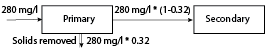
\includegraphics[scale=0.8]{Problem}
\end{center}

Influent BOD concentration to the AS basin: $280\dfrac{mg}{l}*(1-0.32)= 190.4 \dfrac{mg}{l}$\\

$\dfrac{F}{M}= \dfrac{1.5 MGD * 190.4\dfrac{mg}{l}*8.34}{7000*0.79}= \boxed{0.43\dfrac{F}{M}}$
\\

\item Given that an activated sludge plant with an influent flow of 1.2 MGD is operated at an MCRT of 6 days and the parameters below, calculate the WAS flow rate (wasting rate) in gallon per day.
\\

\begin{tabular}{ | m {7 cm} | m {7 cm}| } 
 \hline
Two aeration tanks – 0.5 MG each & Two final clarifiers – 0.25 MG each \\ 
 \hline
 Final effluent $= 20\dfrac{mg}{l}$ & WAS – 7500 ppm\\ 
 \hline
 MLSS –$3600\dfrac{mg}{L}$ & MLSS volatile solids content = 80\%  \\
 \hline
\end{tabular}
\\

MCRT$=\dfrac{lbs MLSS (system)}{\dfrac{lbs}{day}Effluent SS + \dfrac{lbs}{day}WAS SS}  $
\\

\noindent lbs MLSS (system)$=(2*0.5 + 2*0.25)MG * 3600\dfrac{mg}{L} * 8.34 = 45036lbs$
\\

\noindent $\dfrac{lbs}{day} Effluent SS= 1.2 MG * 20\dfrac{mg}{L} * 8.34 = 200.2lbs$
\\

\noindent MCRT: $6 days=\dfrac{45036}{200.2 \dfrac{lbs}{day}+ \dfrac{lbs}{day}WAS SS}  $
\\

\noindent $\dfrac{lbs}{day}WAS SS = \dfrac{45036}{6} - 200.2 = 7306 \dfrac{lbs}{day}$
\\

\noindent $7306 \dfrac{lbs}{day} = WAS Flow (MGD) * 7500 * 8.34 \implies WAS Flow (MGD)=\dfrac{7306}{7500*8.34}=0.116 MGD = \boxed {116,000 \dfrac{gal}{day}}  $







\item Calculate the MCRT of an activated sludge plant given the following information.\\
Plant flow- 4.25 MGD\\
WAS conc-7980 mg/l\\
Waste flow- 0.055 MGD\\
RAS conc.- 7980 mg/l\\
Aeration tank vol-1MG\\  
Clarifier vol- 0.25 MG\\
Final eff TSS conc. - 21.2 mg/l\\
MLSS conc.- 2050 mg/l\\
\vspace{0.3cm}
Solution:\\
\vspace{0.3cm}
$MCRT (days) =  \dfrac{MLSS \enspace in \enspace aeration \enspace tank \enspace (lbs)+MLSS \enspace in \enspace clarifier \enspace (lbs)}{SS \enspace effluent \enspace (lbs/day)+SS \enspace WAS \enspace (lbs/day)}$\\
\vspace{0.3cm} 
$MLSS \enspace in \enspace aeration \enspace tank \enspace (lbs)=1*2050*8.34=17097lbs$\\
\vspace{0.3cm} 
$MLSS \enspace in \enspace clarifier \enspace (lbs)=0.25*2050*8.34=4274.3lbs$\\
\vspace{0.3cm} 
$SS \enspace effluent \enspace (lbs/day)=4.25MGD *21.2mg/l*8.34=751.4lbs/day$\\
\vspace{0.3cm} 
$SS \enspace WAS \enspace (lbs/day)=0.055MGD *7980mg/l*8.34=3660.4lbs/day$\\
\vspace{0.3cm} 
Plugging in the values calculated above: $MCRT (days) =  \dfrac{17097.6+4274.3}{751.4+3660.4}=4.8=\boxed{5days}$\\
\vspace{0.2cm}
\pagebreak

\item Calculate the MCRT given the following.\\
Plant flow - 1.8 MGD\\
MLSS conc -  2800 mg/l\\
WAS flow - 0.04 MGD\\
MLVSS conc. - 2190 mg/l\\
Aerator vol - 0.3 MG\\
Reactor vol. - 0.2 MG\\
RAS conc. - 8150 mg/l\\
Effluent SS conc.-18 mg/l\\
Solution:\\
\vspace{0.2cm}
$MCRT (days) =  \dfrac{MLSS \enspace in \enspace aeration \enspace tank \enspace (lbs)+MLSS \enspace in \enspace clarifier \enspace (lbs)}{SS \enspace effluent \enspace (lbs/day)+SS \enspace WAS \enspace (lbs/day)}$\\
\vspace{0.3cm} 
$MLSS \enspace in \enspace aeration \enspace tank \enspace (lbs)=0.3*2800*8.34=7005.6lbs$\\
\vspace{0.3cm} 
$MLSS \enspace in \enspace clarifier \enspace (lbs)=0.2*2800*8.34=4670.4lbs$\\
\vspace{0.3cm} 
$SS \enspace effluent \enspace (lbs/day)=1.8MGD *18mg/l*8.34=270.2lbs/day$\\
\vspace{0.3cm} 
$SS \enspace WAS \enspace (lbs/day)=0.04MGD *8150mg/l*8.34=2718.8lbs/day$\\
\vspace{0.3cm} 
Plugging in the values calculated above: $MCRT (days) =  \dfrac{7005.6+4670.4}{270.2+2718.8}=3.9=\boxed{4days}$\\
\vspace{0.2cm}
\pagebreak

\item In an aeration tank, the MLSS is 2650 mg/l and recorded 30-minute settling test indicates 221 ml/L.  What is the sludge volume index?\\
\vspace{0.3cm}
Solution:\\
SVI (ml/g)= $\dfrac{Settled \enspace sludge \enspace volume \enspace in \enspace ml/l \enspace after \enspace 30 \enspace min}{MLSS \enspace mg/l}*1000 \dfrac{mg}{g}$\\
\vspace{0.25cm}
SVI=$\dfrac{221ml/l}{2650mg/l}*1000\dfrac{mg}{g}=\boxed{83ml/g}$
\item The desired F/M ratio is .35 lbs BOD/day/lb MLVSS. If 2,100 lbs of BOD enter the aerator daily, how many lbs of MLVSS should be maintained in the aeration tank?\\
Solution:\\
$F:M=\dfrac{(lbs/day) \enspace primary \enspace effluent  \enspace BOD \enspace entering \enspace the  \enspace aeration \enspace tank}{(lbs) \enspace MLVSS \enspace in \enspace the  \enspace aeration \enspace tank}$\\
\vspace{0.3cm}
$\implies 0.35=\dfrac{2100}{x}\implies x = \boxed{130,100lbs \enspace MLVSS}$\\

\item Calculate F/M ratio based on the following data:\\
Secondary influent BOD - 156 mg/l\\
Four (4) aeration basins - 30 ft x 70 ft x 10 ft. deep\\
Influent flow - 0.65 MGD\\
MLSS - 3600 mg/l\\
MLSS average \% volatile - 72\%\\
Solution:\\
\vspace{0.3cm}
$F:M=\dfrac{(lbs/day) \enspace primary \enspace effluent  \enspace BOD \enspace entering \enspace the  \enspace aeration \enspace tank}{(lbs) \enspace MLVSS \enspace in \enspace the  \enspace aeration \enspace tank}$\\
\vspace{0.3cm}
$F:M=\dfrac{156*0.65*8.34}{3600*0.72*4*(30*70*10)ft^3* \dfrac{7.48gal}{ft^3}*\dfrac{MG}{1000000gal}*8.34}=\boxed{0.06}$\\
\pagebreak
\item An activated sludge plant operates well at an F:M ratio of between 0.23 and 0.28.  Calculate the minimum MLSS concentration, given the following:\\
Q = 0.4 MGD\\
Primary influent BOD = 250 mg/l\\
Primary effluent BOD = 128 mg/l\\
Aeration tank vol. = 350,000 gallons\\
Clarifier vol = 250,000 gallons\\
MLSS has 80\% volatile solids\\
Solution:\\
\vspace{0.3cm}
$F:M=\dfrac{(lbs/day) \enspace primary \enspace effluent  \enspace BOD \enspace entering \enspace the  \enspace aeration \enspace tank}{(lbs) \enspace MLVSS \enspace in \enspace the  \enspace aeration \enspace tank}$\\
\vspace{0.3cm}
$\implies F:M \propto \dfrac{1}{MLSS \enspace concentration}$  $\implies$ F:M is inversely proportional to MLSS\\
\vspace{0.3cm}
So to have minimum MLSS conc. F:M needs to be the maximum of the range provided\\
\vspace{0.3cm}
If the MLSS concentration = x:
$ \implies F:M=0.28=\dfrac{0.4*128*8.34}{0.35*x*0.8}\implies x = \boxed{5446 mg/l \enspace MLSS}$
\item 5. Given that an activated sludge plant with an influent flow of 1 MGD is operated at an MCRT of 6 days and the parameters below, calculate the WAS flow rate (wasting rate) in gallon per day.
(10 points)\\
\begin{tabular}{ | m {7 cm} | m {7 cm}| } 
 \hline
Two aeration tanks – 0.45 MG each & Two final clarifiers – 0.2 MG each \\ 
 \hline
 Final effluent $= 16\dfrac{mg}{l}$ & WAS = 6500 ppm\\ 
 \hline
 MLSS =$3000\dfrac{mg}{L}$ & MLSS volatile solids content = 85\%  \\
 \hline
\end{tabular}\vspace{1 cm}
\\
Solution:\\

MCRT$=\dfrac{lbs MLSS (system)}{\dfrac{lbs}{day}Effluent SS + \dfrac{lbs}{day}WAS SS}  $
\\
\vspace{1 cm}
\noindent lbs MLSS (system)$=(2*0.45 + 2*0.2)MG * 3000\dfrac{mg}{L} * 8.34 = 32,526lbs$
\\
\vspace{1 cm}
\noindent $\dfrac{lbs}{day} Effluent SS= 1 MG * 16\dfrac{mg}{L} * 8.34 = 133.4lbs$
\\
\vspace{1 cm}
\noindent MCRT: $6 days=\dfrac{32,526}{133.4 \dfrac{lbs}{day}+ \dfrac{lbs}{day}WAS SS}  $
\\
\vspace{1 cm}
\noindent $\dfrac{lbs}{day}WAS SS = \dfrac{32,526}{6} - 133.4 = 5,288 \dfrac{lbs}{day}$
\\
\vspace{1 cm}
\noindent $5,288 \dfrac{lbs}{day} = WAS Flow (MGD) * 6500 * 8.34$\\
\vspace{1 cm}
$\implies WAS Flow (MGD)=\dfrac{5,288}{6,500*8.34}=0.097546 MGD = \boxed {97,546 \dfrac{gal}{day}}$

\item Operational data is given below for a conventional activated sludge treatment plant:\\

Influent flow: 2.5 mgd\\
Influent BOD: 220 mg/l\\
Influent TSS: 240 mg/l\\
Primary BOD removal efficiency: 30\%\\
Aeration tank volume: 1.8 MG\\
Secondary clarifier volume: 0.8 MG\\
MLSS: 3,600 mg/l\\
MLVSS: 2,800 mg/l\\
RAS SS: 8,500 mg/l\\
RAS VSS: 6,630 mg/l\\
RAS flow: 100\%\\
WAS flow: 35,000 gpd\\
AS Effluent TSS: 25 mg/l\\
AS Effluent BOD: 19 mg/l\\
Settleability results: 60 min= 300 ml/L\\
Settleability results: 30 min= 320 ml/L\\

\begin{enumerate}
\item Calculate the MCRT
\item Calculate the F/M Ratio
\item Calculate the SVI
\end{enumerate}

Solution:\\
\vspace{0.3cm}
\begin{enumerate}
\item $MCRT (days) =  \dfrac{MLSS \enspace in \enspace aeration \enspace tank \enspace (lbs)+MLSS \enspace in \enspace clarifier \enspace (lbs)}{SS \enspace effluent \enspace (lbs/day)+SS \enspace WAS \enspace (lbs/day)}$\\
\vspace{0.3cm} 
$MLSS \enspace in \enspace aeration \enspace tank \enspace (lbs)=1.8*3,600*8.34=54,043lbs$\\
\vspace{0.3cm} 
$MLSS \enspace in \enspace clarifier \enspace (lbs)=0.8*3,600*8.34=24,019lbs$\\
\vspace{0.3cm} 
$SS \enspace effluent \enspace (lbs/day)=2.5MGD *25mg/l*8.34=521lbs/day$\\
\vspace{0.3cm} 
$SS \enspace WAS \enspace (lbs/day)=\dfrac{35,000}{1,000,000}MGD *8,500mg/l*8.34=2,481lbs/day$\\
\vspace{0.3cm} 
$MCRT (days) =  \dfrac{54,043+24,019}{521+2,481}=\boxed{26 \enspace days}$\\
\vspace{0.2cm}
\item $F:M=\dfrac{(lbs/day) \enspace primary \enspace effluent  \enspace BOD \enspace entering \enspace the  \enspace aeration \enspace tank}{(lbs) \enspace MLVSS \enspace in \enspace the  \enspace aeration \enspace tank}$\\
\vspace{0.3cm}
$F:M=\dfrac{220*(1-0.3)*2.5*8.34}{1.8*2,800*8.34}=\boxed{0.08}$\\
\vspace{0.25cm}

\item SVI (ml/g)= $\dfrac{Settled \enspace sludge \enspace volume \enspace in \enspace ml/l \enspace after \enspace 30 \enspace min}{MLSS \enspace mg/l}*1000 \dfrac{mg}{g}$\\
\vspace{0.25cm}
SVI=$\dfrac{320ml/l}{3,600mg/l}*1000\dfrac{mg}{g}=\boxed{89ml/g}$
\end{enumerate}

\item What is the Sludge Volume Index given the following:\\  MLSS = 2800 mg/l; MLVSS 2400 mg/l; Settled Volume after 30 minutes = 250 ml/L\\
\vspace{0.3cm} 
Solution:\\
SVI (ml/g)= $\dfrac{Settled \enspace sludge \enspace volume \enspace in \enspace ml/l \enspace after \enspace 30 \enspace min}{MLSS \enspace mg/l}*1000 \dfrac{mg}{g}$\\
\vspace{0.25cm}
SVI=$\dfrac{250ml/l}{2800mg/l}*1000\dfrac{mg}{g}=\boxed{89ml/g}$

\item Plant Influent Flow:  3.5 MGD\\
Plant Influent BOD:  276 mg/l\\
Primary Treatment BOD Removal:  36\%\\
Desired F/M:  0.3\\
Find lbs of MLVSS that should be maintained in the activated sludge treatment process. (Answer: 17,187 lbs)

\item Given that an activated sludge plant with an influent flow of 1 MGD is operated at an MCRT of 6 days and the parameters below, calculate the WAS flow rate (wasting rate) in gallon per day\\
\begin{tabular}{ | m {7 cm} | m {7 cm}| } 
 \hline
Two aeration tanks – 0.45 MG each & Two final clarifiers – 0.2 MG each \\ 
 \hline
 Final effluent $= 16\dfrac{mg}{l}$ & WAS = 6500 ppm\\ 
 \hline
 MLSS =$3000\dfrac{mg}{L}$ & MLSS volatile solids content = 85\%  \\
 \hline
\end{tabular}\vspace{1 cm}
\\
(Answer: 97,546 gal/day)

\item The aeration tank of a conventional activated sludge plant contains 9300 Ibs of MLSS.  Lab tests show that the MLSS are 79\% volatile solids. The primary effluent contains 2900 Ibs of BOD.  Calculate the F to M ratio for this wastewater treatment plant. (Answer:  0.4)

\item How many lbs of solids are in a 400,000 gallon aeration tank if the suspended solids concentration is 1200 mg/l? (Answer: 4003 lbs)



\item An activated sludge wastewater treatment plant treats an average flow of 3.25 MGD. The aeration tank has a volume of 1.0 MG and a MLSS concentration of 2100 mg/l. The final clarifier has an operating volume of 0.25 MG. Effluent suspended solids concentration averages 21.2 mg/l. The WAS concentration is 8100 mg/l and is wasted at the rate of 0.055 MGD. Calculate the MCRT.

\item What is the F/M ratio on an aeration tank if 1,500 pounds of BOD are added per day and 5000 pounds of volatile solids are under aeration? 

\item In an aeration tank, the MLSS is 2500 mg/l and recorded 30-minute settling test indicates 230 ml.  What is the sludge volume index?



\item An activated sludge aeration tank receives a primary effluent flow of 2.61 MGD with a BOD concentration of 195 mg/l. The mixed liquor volatile suspended solids concentration is 2560 mg/l and the aeration tank volume is 470,000 gallons. What is the current F/M ratio?

\item Calculate the MCRT given the following.
Plant flow- 2.8 MGD\\ 		MLSS conc.- 2800 mg/l\\
WAS flow- 0.07 MGD\\ 		MLVSS conc.- 2190mg/l\\
Aerator volume - 0.38MG\\	RAS SS concentration - 6800 mg/l\\
Clarifier volume - 0.19 MG\\ 	Final effluent TSS - 18 mg/l\\


\item If in a conventional activated sludge treatment plant the aeration tank contains 7000 lbs of MLSS and the final clarifier contains 2500 lbs of MLSS.  If 1300 lbs of solids are wasted each day and 120 lbs of solids leave in the final effluent, Calculate the MCRT.

\item The aeration tank of a conventional activated sludge plant contains 9300 Ibs of MLSS. Lab tests show that the MLSS are 79\% volatile solids. The primary effluent contains twenty-nine hundred pounds (2900 Ibs) of BOD. Calculate the F to M ratio for this wastewater treatment plant.




\item A conventional activated sludge plant receives an average flow of 2.5 MGD. The influent BOD averages 230 and the primary effluent BOD average 160 mg/I. The 0.6 MG aeration tank has a MLSS cone. of 2800 mg/l and a MLVSS cone. of 21 50 mg/l. Calculated the F to M ratio for this plant.




\item A convention activated sludge plant receives an average influent flow of 800,000 gpd. The influent BOD averages 200 mg/l and on the average 32\% of this BOD is removed in the primary sedimentation tank. The mixed liquor tank contains 3250 Ibs of MLSS. These solids contain 77\% volatile matter. Calculate this plant's F to M ratio.

\item In an conventional activated sludge plant calculations show that the aeration tank contains 6500 Ibs of MLSS and the final clarifier contains 2500 Ibs of MLSS. Twelve hundred and fifty pounds (1250 Ibs) of solids is wasted each day and 100 Ibs/day of solids leave in the final effluent. Calculate the MCRT for this plant.


\item A activated sludge plant has a total of 25,000 pounds of solids in the system (i.e. aerator + final clarifier) and has an average effluent flow of 3.75 MGD. The effluent suspended solids concentration averages 22 mg/l. The WAS has a concentration of 7500 mg/l and is being wasted at 0.05 MGD. Calculate the MCRT.


\item An activated sludge wastewater treatment plant discharges an average flow of 3.25· MGD. The mixed liquor tank has a volume of 1.0 MG and a MLSS concentration of 2100 mg/l. The final clarifier has an operating volume of 0.25 MG. Effluent suspended solids concentration averages 21.2 mg/l. The WAS concentration is 8100 j mg/l and is wasted at the rate of 0.055 MGD. Calculate the MCRT.

\item In an conventional activated sludge plant show that the aeration tank contains 6500 Ibs of MLSS and the final clarifier contains 2500 lbs of MLSS. 1250 Ibs of solids is wasted each day and 100 Ibs/day of solids leave in the final effluent. Calculate the MCRT for this plant.  Answer:  7 days

\item An activated sludge plant has a total of 25,000 pounds of solids in the system (aerator + final Clarifier) and has an average effluent flow of 3.75 MGD. The effluent suspended solids concentration averages 22 mg/l. The WAS has a concentration 'of 7500 .mg/l and is being wasted at 0.05 MGD. Calculate the MCRT.  Answer:  7 days

\item An activated sludge wastewater treatment plant discharges an average flow of 3.25 MGD. The mixed liquor tank has a volume of 1.0 MG and a MLSS concentration of 2100 mg/l. The final clarifier has an operating volume of 0.25 MG. Effluent suspended solids concentration averages 21.2 mg/l and the WAS concentration is 8100 mg/l and is wasted at the rate of 0.055 MGD.  Calculate the MCRT.  Answer: 5.1 days

\item A conventional activated sludge plant receives an average flow of 2.5 MGD. The influent BOD averages 230 and the primary effluent BOD averages 160mg/l The 0.6 MG aeration tank has a MLSS conc. of 2800 mg/l and a MLVSS conc. of 2150mg/l. Calculate  the F to M ratio for this plant.  Answer:  0.31

\item A conventional activated sludge plant receives an influent flow of 800,000 gpd. The influent BOD averages 200 mg/l and on the average 32\% of this BOD is removed in the primary sedimentation tank. The mixed liquor tank contains 3250 Ibs of MLSS. These solids contain 77\% volatile matter. Calculate this plant's F to M ratio.  Answer:  0.36

\item Calculate the MCRT given the following.
Plant flow- 1.8 MGD\\ 		MLSS conc.- 2800 mg/l\\
WAS flow- 0.04 MGD \\		MLVSS conc.- 2190mg/l\\
Aerator vol- 0.3MG\\	RAS conc.- 8150 mg/l\\
Clarifier vol- 0.lMG\\ 		Final eff TSS- 26 mg/l\\
Answer: 3 days

\item Calculate the F to M ratio given the following Information.
Plant flow- 3.7 MGD\\		Primary eff TSS- 120mg/l\\
Aerator Vol - 0.85 MG\\ 	MLSS conc.- 3200 mg/l\\
Clarifier Vol - 0.25 MG \\	MLVSS conc.- 2550 mg/l\\
Primary effluent BOD-120 mg/l\\
Answer:  0.2\\

\item Calculate the F to M ratio given the following.
Plant flow- 0.8 MGD
Aerator vol- 200,000 gal.
Clarifier Volume-175,000 gal
Primary eff BOD- 120 mg/l
MLVSS cone. -1950 mg/l\\
Answer:  0.25\\
\vspace{0.3cm}
$F:M=\dfrac{(lbs/day) \enspace primary \enspace effluent  \enspace BOD \enspace entering \enspace the  \enspace aeration \enspace tank}{(lbs) \enspace MLVSS \enspace in \enspace the  \enspace aeration \enspace tank}$\\
\vspace{0.3cm}
$F:M=\dfrac{120*0.8*8.34}{1950*0.2*8.34}=\boxed{0.25}$\\
\item Calculate the MCRT of an activated sludge plant given the following information.
Plant flow- 4.25 MGD\\
WAS conc-7980 mg/l\\
Waste flow- 0.055 MGD\\
RAS conc.- 7980 mg/l\\
Aeration tank vol-1MG\\  
Clarifier vol- 0.25 MG\\
Final eff TSS conc. - 21.2 mg/l\\
MLSS conc.- 2050 mg/l\\
$MCRT (days) =  \dfrac{MLSS \enspace in \enspace aeration \enspace tank \enspace (lbs)+MLSS \enspace in \enspace clarifier \enspace (lbs)}{SS \enspace effluent \enspace (lbs/day)+SS \enspace WAS \enspace (lbs/day)}$\\
\vspace{0.3cm} 
$MLSS \enspace in \enspace aeration \enspace tank \enspace (lbs)=1*2050*8.34=17097lbs$\\
\vspace{0.3cm} 
$MLSS \enspace in \enspace clarifier \enspace (lbs)=0.25*2050*8.34=4274.3lbs$\\
\vspace{0.3cm} 
$SS \enspace effluent \enspace (lbs/day)=4.25MGD *21.2mg/l*8.34=751.4lbs/day$\\
\vspace{0.3cm} 
$SS \enspace WAS \enspace (lbs/day)=0.055MGD *7980mg/l*8.34=3660.4lbs/day$\\
\vspace{0.3cm} 
Plugging in the values calculated above: $MCRT (days) =  \dfrac{17097.6+4274.3}{751.4+3660.4}=4.8=\boxed{5days}$\\
\vspace{0.2cm}


\item Calculate the MCRT given the following.\\
Plant flow - 1.8 MGD\\
MLSS conc -  2800 mg/l\\
WAS flow - 0.04 MGD\\
MLVSS conc. - 2190 mg/l\\
Aerator vol - 0.3 MG\\
Reactor vol. - 0.2 MG\\
RAS conc. - 8150 mg/l\\
Effluent SS conc.-18 mg/l\\
Solution:\\
\vspace{0.2cm}
$MCRT (days) =  \dfrac{MLSS \enspace in \enspace aeration \enspace tank \enspace (lbs)+MLSS \enspace in \enspace clarifier \enspace (lbs)}{SS \enspace effluent \enspace (lbs/day)+SS \enspace WAS \enspace (lbs/day)}$\\
\vspace{0.3cm} 
$MLSS \enspace in \enspace aeration \enspace tank \enspace (lbs)=0.3*2800*8.34=7005.6lbs$\\
\vspace{0.3cm} 
$MLSS \enspace in \enspace clarifier \enspace (lbs)=0.2*2800*8.34=4670.4lbs$\\
\vspace{0.3cm} 
$SS \enspace effluent \enspace (lbs/day)=1.8MGD *18mg/l*8.34=270.2lbs/day$\\
\vspace{0.3cm} 
$SS \enspace WAS \enspace (lbs/day)=0.04MGD *8150mg/l*8.34=2718.8lbs/day$\\
\vspace{0.3cm} 
Plugging in the values calculated above: $MCRT (days) =  \dfrac{7005.6+4670.4}{270.2+2718.8}=3.9=\boxed{4days}$\\
\vspace{0.2cm}

\item The desired F/M ratio is .35 lbs BOD/day/lb MLVSS. If 2,100 lbs of BOD enter the aerator daily, how many lbs of MLVSS should be maintained in the aeration tank?\\
Solution:\\
$F:M=\dfrac{(lbs/day) \enspace primary \enspace effluent  \enspace BOD \enspace entering \enspace the  \enspace aeration \enspace tank}{(lbs) \enspace MLVSS \enspace in \enspace the  \enspace aeration \enspace tank}$\\
\vspace{0.3cm}
$\implies 0.35=\dfrac{2100}{x}\implies x = \boxed{6000lbs \enspace MLVSS}$\\

\item Calculate F/M ratio based on the following data:\\
Secondary influent BOD - 156 mg/l\\
Four (4) aeration basins - 30 ft x 70 ft x 10 ft. deep\\
Influent flow - 0.65 MGD\\
MLSS - 3600 mg/l\\
MLSS average \% volatile - 72\%\\
Solution:\\
\vspace{0.3cm}
$F:M=\dfrac{(lbs/day) \enspace primary \enspace effluent  \enspace BOD \enspace entering \enspace the  \enspace aeration \enspace tank}{(lbs) \enspace MLVSS \enspace in \enspace the  \enspace aeration \enspace tank}$\\
\vspace{0.3cm}
$F:M=\dfrac{156*0.65*8.34}{3600*0.72*4*(30*70*10)ft^3* \dfrac{7.48gal}{ft^3}*\dfrac{MG}{1000000gal}*8.34}=\boxed{0.06}$\\
\vspace{0.3cm}
\item An activated sludge plant operates well at an F:M ratio of between 0.23 and 0.28.  Calculate the minimum MLSS concentration, given the following:
Q = 0.4 MGD
Primary influent BOD = 250 mg/l
Primary effluent BOD = 128 mg/l
Aeration tank vol. = 350,000 gallons
Clarifier vol = 250,000 gallons
MLSS has 80\% volatile solids
Solution:\\
\vspace{0.3cm}
$F:M=\dfrac{(lbs/day) \enspace primary \enspace effluent  \enspace BOD \enspace entering \enspace the  \enspace aeration \enspace tank}{(lbs) \enspace MLVSS \enspace in \enspace the  \enspace aeration \enspace tank}$\\
\vspace{0.3cm}
$\implies F:M \propto \dfrac{1}{MLSS \enspace concentration}$\\
\vspace{0.3cm}
So to have minimum MLSS conc. F:M needs to be the maximum of the range provided\\
\vspace{0.3cm}
If the MLSS concentration = x:
$ \implies F:M=0.28=\dfrac{0.4*128*8.34}{0.35*x*0.8}\implies x = \boxed{5446 mg/l \enspace MLSS}$







\item If the target MCRT for an activated sludge plant with the following parameters is 8 days, what is the required wasting rate (in gallons per day)? (8 points)

Aeration Tank Volume = 1.5 MG\\
Clarifier Volume = 1.2 MG\\
MLSS Concentration = 2500 mg/l\\
MLSS Volatile Solids = 79\%\\
WAS SS = 5100 mg/l\\
Secondary Effluent SS = 12 mg/l\\
Plant flow = 15 MGD\\
$ MCRT = \dfrac{(Total \enspace MLSS \enspace lbs \enspace in \enspace the \enspace aeration \enspace system (aeration \enspace tank\enspace+\enspace clarifier))}{(Total \enspace amount \enspace in \enspace \dfrac{lbs}{day} \enspace of \enspace  SS \enspace leaving \enspace the  \enspace system (effluent+WAS))}$\\
$MCRT =\dfrac{(MLSS\textsubscript{aeration tank} (lbs)\enspace + \enspace MLSS \textsubscript{clarifier} \enspace (lbs))}{(SS \textsubscript{effluent} (lbs/day)+SS \textsubscript{WAS} (lbs/day))}$\\

$\implies 8 days=\dfrac{(1.5 + 1.2)MG * 8.34 * 2500 \dfrac{mg}{l}}{(15 MGD*12\dfrac{mg}{l} *8.34) (lbs/day \enspace SS \textsubscript{effluent}+(xMGD \enspace WAS * 5100\dfrac{mg}{l}*8.34)(lbs/day \enspace SS \textsubscript{WAS})}$

$(15 *12*8.34 (lbs/day)SS \textsubscript{effluent}+xMGD\enspace WAS * 5100*8.34)(lbs/day)SS \textsubscript{WAS}=\dfrac{(1.5 + 1.2)MG * 8.34 * 2500}{8}$

$xMGD\enspace WAS * 5100*8.34(lbs/day)SS \textsubscript{WAS}=\dfrac{(1.5 + 1.2)MG * 8.34 * 2500}{8}-(15 *12*8.34 (lbs/day)SS \textsubscript{effluent}$\\
$42,534x=5535.7\implies x =\dfrac{5535.7}{42,534}=0.1301 MGD = \boxed{130,100\dfrac{gal}{day}}$\\
\vspace {8mm}

\item Given the following:
Plant Influent Flow:  3.5 MGD\\
Plant Influent BOD:  276 mg/l\\
Primary Treatment BOD Removal:  36\%\\
Desired F/M:  0.3\\
Find lbs of MLVSS that should be maintained in the activated sludge treatment process. (7 points)
$F:M = \dfrac{lbs \enspace Influent \enspace BOD}{lbs \enspace MLVSS}\implies 0.3 = \dfrac{276*(1-0.36)*3.5*8.34}{lbs MLVSS} \implies lbs \enspace MLVSS=\boxed{17,187lbs}$

5. Given that an activated sludge plant with an influent flow of 1 MGD is operated at an MCRT of 6 days and the parameters below, calculate the WAS flow rate (wasting rate) in gallon per day.
(10 points)\\
\begin{tabular}{ | m {7 cm} | m {7 cm}| } 
 \hline
Two aeration tanks – 0.45 MG each & Two final clarifiers – 0.2 MG each \\ 
 \hline
 Final effluent $= 16\dfrac{mg}{l}$ & WAS = 6500 ppm\\ 
 \hline
 MLSS =$3000\dfrac{mg}{L}$ & MLSS volatile solids content = 85\%  \\
 \hline
\end{tabular}\vspace{1 cm}
\\
Solution:\\

MCRT$=\dfrac{lbs MLSS (system)}{\dfrac{lbs}{day}Effluent SS + \dfrac{lbs}{day}WAS SS}  $
\\
\vspace{1 cm}
\noindent lbs MLSS (system)$=(2*0.45 + 2*0.2)MG * 3000\dfrac{mg}{L} * 8.34 = 32,526lbs$
\\
\vspace{1 cm}
\noindent $\dfrac{lbs}{day} Effluent SS= 1 MG * 16\dfrac{mg}{L} * 8.34 = 133.4lbs$
\\
\vspace{1 cm}
\noindent MCRT: $6 days=\dfrac{32,526}{133.4 \dfrac{lbs}{day}+ \dfrac{lbs}{day}WAS SS}  $
\\
\vspace{1 cm}
\noindent $\dfrac{lbs}{day}WAS SS = \dfrac{32,526}{6} - 133.4 = 5,288 \dfrac{lbs}{day}$
\\
\vspace{1 cm}
\noindent $5,288 \dfrac{lbs}{day} = WAS Flow (MGD) * 6500 * 8.34$\\
\vspace{1 cm}
$\implies WAS Flow (MGD)=\dfrac{5,288}{6,500*8.34}=0.097546 MGD = \boxed {97,546 \dfrac{gal}{day}}$

\item The desired F/M ratio is 0.35. If 2,100 lbs of BOD enter the aerator daily and the volume of the mixed liquor in the aeration tank is 375,000 gallons , what should be the target MLVSS concentration?\\

Solution:\\
$F:M=\frac{(lbs/day) \enspace primary \enspace effluent  \enspace BOD \enspace entering \enspace the  \enspace aeration \enspace tank}{(lbs) \enspace MLVSS \enspace in \enspace the  \enspace aeration \enspace tank}$\\
\vspace{0.3cm}
$\implies 0.35=\frac{2100}{x}\implies x = \boxed{6000lbs \enspace MLVSS}$\\

\vspace{0.3cm}
$\implies 6,000 lbs \enspace MLVSS=8.34 * \frac{375,000}{1,000,000}MG*x\frac{mg \enspace MLVSS}{L}$\\
$\implies x\frac{mg \enspace MLVSS}{L} = \frac{6000}{8.34*0.375}=\boxed{1,900\frac{mg \enspace MLVSS}{L}}$






























\end{enumerate}


\section*{Solids Treatment Math Problems}
\begin{enumerate}
\item Calculate the volatile solids reduction in an anaerobic digester given the following information: Raw sludge feed to digester: 73.7 \% VS and digested sludge: 57.2 \%VS\\

*a. 52.3\% \\
b. 64\%\\
c. 16.5\% \\
d. 42\% \\
\vspace{0.25cm}
Solution:\\
\vspace{0.25cm}  
The VS reduction of the digester is provided by the Van Kleeck equation \\ 
\vspace{0.25cm}
$Digester \enspace VS \enspace reduction (\%)=\dfrac{VS_{in}-VS_{out}}{VS_{in}-VS_{in}*VS_{out}}*100$\\
\vspace{0.25cm}
$Digester \enspace VS \enspace reduction (\%)=\dfrac{0.737-0.572}{0.737-0.737*0.572}*100=\boxed{ 52.3\%}$\\





\item 42,000 gallons of 6\% sludge containing 67\% volatile matter is pumped to the digester.  The digester reduces the volatile matter by 52\%.  What volume of sludge in gallons containing 5\% solids remains after digestion? [Ans:  32,841 gal]

\item An anaerobic digester is 37’ in diameter and 27’ deep with a 5,000 gallon daily sludge flow. The sludge is 6\% solids and 66\% volatile solids.  What is the volatile solids loading in pounds per cubic foot per day? [0.057 lbs VS/ft3-day]

\item An Imhoff cone result is 5.5 ml/l.  Approximately how many gallons of primary sludge will need to be pumped if the flow is 0.7 MGD? [3,850 gallons]

\item A sludge digester equipped with a floating cover is 31 ft. inside diameter.  The corbels are 16 feet above the floor and the top of the wall is 20 feet above the floor.  The digester currently has a sludge depth of 16.5 ft. How many gallons of sludge are needed to displace the cover 1 foot? [5,643 galllons]

\item 10,000 gallons/day of sludge is pumped to an anaerobic digester/day at 4\% solids (70\% VS).  If 50\% of the VS is destroyed, how many lbs of VS is destroyed per day?\\
Solution:\\
$\frac{10,000 \enspace Gal}{day}*\frac{8.34 \enspace lbs \enspace sludge}{Gal} \frac{0.04*0.7 \enspace lbs \enspace VS \enspace feed}{lb \enspace sludge}*\frac{0.5 \enspace lbs \enspace VS \enspace destroyed}{lbs \enspace VS \enspace feed}=\boxed{\frac{1,168lbs \enspace VS \enspace destroyed}{day} } $


\item Two sludges are blended together as follows: 15,000 gal. primary sludge at 4.1\% solids. 28,000 gal. secondary sludge at 1.3\% solids. What is the combined solids concentration? [Ans. 2.28\%] If the primary sludge is 68\% VS and the secondary sludge is 63\% VS, how many pounds of VS are in the combined sludge? [Ans. 5400.3 lbs VS]


\item 12,000 gallons of 1.8\% sludge is pumped to a thickener, and is thickened to 3800 gallons of 4.9\% solids. The supernatant is returned back to the head of the STP for treatment.  What is the volume in gallons and solids concentration in ppm of the supernatant?[Ans. 24,980 gallons]


\item How many pounds of solids are pumped to a digester each day if the digester receives 10,000 gpd of sludge at 5\% solids concentration?\\


 

Solution:\\

{
$
	\dfrac{lbs \enspace TS}{day}
	=
	\dfrac{10,000 gal \enspace sludge}{day}
	*
	\dfrac{(8.34*0.05 lbs TS )}{gal \enspace sludge}
	=4,170
	\dfrac{lbs \enspace TS}{day}
$
}\\


\item Calculate the \% VS reduction in a digester given the volatile solids content of the influent sludge to the digester is 70\% and the volatile solids content of the sludge leaving the digester is 52.5\%\\
Solution:  $Digester \enspace VS \enspace reduction (\%)=\dfrac{0.7-0.525}{0.7-0.7*0.525}*100=\boxed{ 53\%}$\\

\item If an anaerobic digester receives sludge with VS of 80\% and discharges digested sludge with a 60\% VS. Its VS reduction is:\\
a. 20\% \\
b. 25\% \\
c. 63\% \\
d. 89\% \\
\vspace{0.25cm}
Solution:\\
\vspace{0.25cm}
$Digester \enspace VS \enspace reduction (\%)=\dfrac{0.8-0.6}{0.8-0.8*0.6}*100=\boxed{ 63\%}$\\

\vspace{0.25cm}
\item Calculate the VS loading to the digester in lbs/day if 10,000 gallons of sludge containing 5\% TS with and average VS content of 78\%\\
Solution:\\
Digester VS loading (lbs/day)\\$=\dfrac{10,000 \enspace gallons \enspace sludge}{day}*\dfrac{8.34lbs \enspace sludge}{gal}*\dfrac{0.05*0.78lbs VS}{lb \enspace sludge}=\boxed{3,253lbs \enspace sludge \enspace per \enspace day}$

\item Primary sludge containing five percent (5\%) solids is pumped to a digester continuously at a rate of 25 gpm. How many pounds of volatile solids are added to the digester each day if the volatile solids content is 73\% of the total solids?\\
a. 1,310 lbs/day \\
b. 1,800 lbs/day \\
c. 9,830 lbs/day \\
d. 10,960 lbs/day \\
e. 15,010 lbs/day \\
\vspace{0.25cm}
Solution:\\
\vspace{0.25cm}
Digester VS loading (lbs/day)\\$=\dfrac{25*1,440 \enspace gallons \enspace sludge}{day}*\dfrac{8.34lbs \enspace sludge}{gal}*\dfrac{0.05*0.73lbs VS}{lb \enspace sludge}=\boxed{10,960 \enspace lbs \enspace sludge \enspace per \enspace day}$\\
\vspace{0.25cm}






\item An anaerobic digester is 37’ in diameter and 27’ deep with a 5,000 gallon daily sludge flow. The sludge is 6\% solids and 66\% volatile solids.  What is the volatile solids loading in pounds per cubic foot per day?
	
	
Solution:\\
{
$
	Digester \enspace volatile \enspace solids 			\enspace loading \enspace rate = 					\dfrac
	{
	Digester \enspace Loading 
		\dfrac
		{
		lbs \enspace VS
		}
		{
		day
		}
	}
	{
	Digester \enspace volume (V)ft^3
	}
$
}\\
\begin{center}
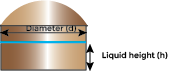
\includegraphics[scale=1]{DigesterWOCDimensions_1}
\end{center}

{
$=\dfrac
	{
		5000
		\dfrac
			{gal \enspace sludge}
			{day}
		*(8.34*0.06*0.66) 
		\dfrac
			{lbs VS}
			{gal \enspace  sludge}
	}
	{
		(\dfrac
			{\pi}
			{4}*37^2*27)ft^3
	}
=\boxed
	{
		0.057 \dfrac
			{lbs \enspace VS}
			{day-ft^3}
	}
$}


\item How much gas is produced in the above digester in $ft^3$/day if the digested sludge contains 2.5\% total solids of which 59\% is volatile solids and the gas production rate is 14 $ft^3$/lb VS destroyed?\\
Solution:\\

{
$
Digester \enspace VS \enspace reduction (\%)=
	\dfrac
	{0.70 - .59}
	{0.70 - 0.70 *0.59}
	*100=38.3\%
$
}\\
\vspace{6mm}

{
$
	\dfrac
	{
	lbs \enspace VS \enspace reduction
	}
	{
	day
	}
	=
	\dfrac
	{
	3153 lbs \enspace VS \enspace feed
		*  0.383 \enspace VS \enspace reduction
	}
	{
	day
	}
 	=1,208
	\dfrac
	{
	lbs \enspace VS \enspace reduction
	}
	{
	day 
	}
$
}\\
\vspace{6mm}

{
$
	\dfrac 
	{
	ft^3 gas \enspace produced
	}
	{
	day
	}
	=
	1208 \dfrac
			{
			lbs \enspace VS \enspace reduced
			}
			{
			day
			}
			*
		\dfrac
		{
		14 ft^3 \enspace gas \enspace produced
		}
		{
		lb \enspace VS \enspace reduced
		}
		=16,912 \dfrac
				{
				ft^3 \enspace digester \enspace 					gas \enspace produced
				}
				{
				day
				}
$
} 
\item The sludge feed to a digester is 80,000 gal/day. The sludge contains 4.5\% total solids with 75\% volatile solids. If 50\% of VS are reduced in the digester: 



\begin{enumerate}
\item Find lbs VS destroyed per 1000 gal of digester capacity per day if the digester radius is 55 ft with an operating sludge level of 25 ft.(5 points)

\vspace{1cm}
Solution:\\
Digester Volume: 
$
{
		(\pi*55^2*25)ft^3 *7.48 \dfrac{gal}{ft^3}
	}=1,776,220 gallons=1,776.2 \enspace(1000 \enspace gallons)
$
\\
\vspace{3mm}
$
	\dfrac
	{
	lbs \enspace VS \enspace reduction
	}
	{
	day
	}
	=
	\dfrac
	{
	80,000 gal * 8.34 \dfrac{lbs}{gal}*(0.045*0.75) \dfrac{lbs VS}{lb}*0.5\dfrac{lbs \enspace VS \enspace  reduction}{lb \enspace VS}
	}
	{
	day
	}$\\
\vspace{0.25cm}
$
 	=11,259
	\dfrac
	{
	lbs \enspace VS \enspace reduction
	}
	{
	day 
	}
$
\\
\vspace{3mm}


$
	\dfrac
	{
	lbs \enspace VS \enspace reduction
	}
	{
	1000 \enspace digester \enspace capacity
	}
	=
	\dfrac
	{
	11,259 \dfrac
			{
			lbs \enspace VS \enspace reduction
			}
			{
			day
			}
	}
	{	
	1,776.2 \enspace (1000 \enspace gallons)
	}
 	=\boxed{6.3
	\dfrac
	{
	lbs \enspace VS \enspace reduction
	}
	{
	1000 gallons \enspace digester \enspace volume 
	}}
$
\\

\vspace{1cm}

\item  What is the digester gas production in Btu/day? Assume 14 cu. ft digester gas per lb of VS destroyed and a 650 Btu/cu. ft heating value for the digester gas produced (5 points)
\end{enumerate}
\vspace{1cm}
Solution:\\

$
	\dfrac 
	{
	ft^3 gas \enspace produced
	}
	{
	day
	}
	=
	11,259 \dfrac
			{
			lbs \enspace VS \enspace reduced
			}
			{
			day
			}
			*
		\dfrac
		{
		14 ft^3 \enspace gas \enspace produced
		}
		{
		lb \enspace VS \enspace reduced
		}
		=157,626 \dfrac
				{
				ft^3 \enspace digester \enspace 					gas \enspace produced
				}
				{
				day
				}
$
\\
\vspace{1cm}


$
	\dfrac 
	{
	BTU \enspace produced
	}
	{
	day
	}
	=
	157,626 \dfrac
			{
			ft^3 \enspace gas \enspace produced
			}
			{
			day
			}
			*
		\dfrac
		{
		650 BTU \enspace gas \enspace produced
		}
		{
		ft^3 gas
		}
		=\boxed{102,456,900 \dfrac
				{
				BTU \enspace produced
				}
				{
				day
				}}
$



\item The volatile acids concentration of sludge in an anaerobic digester is 195 mg/l. If the maximum volatile acids:alkalinity ratio is 0.087, what should the alkalinity be in mg/l?\\
Solution:\\
Volatile acid:Alkalinity=0.087=$\dfrac{195}{x}\implies x = \dfrac{195}{0.087} =\boxed{2,241\dfrac{mg}{l}}$
\pagebreak
	
\item 10,000 gallons of sludge is pumped to an anaerobic digester/day at 4\% solids (70\% VS).  50\% of the VS are destroyed, creating 15 $ft^3$ of gas per lbs. of VS destroyed. How much gas is produced each day?\\

{
$
	\dfrac
	{
	lbs \enspace VS \enspace reduction
	}
	{
	day
	}
	=
	\dfrac
	{
	10,000 gal * 8.34 \dfrac{lbs}{gal}*(0.04*0.7) \dfrac{lbs VS}{lb}*\dfrac{0.5 lbs \enspace VS \enspace  reduction}{lb \enspace VS}
	}
	{
	day
	}
 	=1,168
	\dfrac
	{
	lbs \enspace VS \enspace reduction
	}
	{
	day 
	}
$
}\\
\vspace{3mm}

{
$
	\dfrac 
	{
	ft^3 gas \enspace produced
	}
	{
	day
	}
	=
	1,168 \dfrac
			{
			lbs \enspace VS \enspace reduced
			}
			{
			day
			}
			*
		\dfrac
		{
		15 ft^3 \enspace gas \enspace produced
		}
		{
		lb \enspace VS \enspace reduced
		}
		=17,520 \dfrac
				{
				ft^3 \enspace digester \enspace 					gas \enspace produced
				}
				{
				day
				}
$
} 


\item Given a sludge flow of 5,500 gpd with 6.5\% solids containing  72\% VS to a digester with a VS destruction of 48\%   If the digester is digester is 40 ft. diameter with a sludge level of 25 ft, find lbs. VS destroyed per 1000 gal of digester capacity per day.  What is the digester gas production in Btu/day if the \% VS reduction in the digester is 58\% and the digester raw sludge feed is 6000 cu. Ft/day containing 4.5\% total solids with a 64\% VS content?  Assume 13.5 cu. ft digester gas per lb of VS destroyed and a 650 Btu/cu. ft heating value for the digester gas produced\\

{
Digester Volume: 
$
{
		(\dfrac
			{\pi}
			{4}*40^2*25)ft^3 *7.48 \dfrac{gal}{ft^3}
	}=940,086 gallons=940 \enspace(1000 \enspace gallons)
$
}\\
\vspace{3mm}

{
$
	\dfrac
	{
	lbs \enspace VS \enspace reduction
	}
	{
	day
	}
	=
	\dfrac
	{
	5,500 gal * 8.34 \dfrac{lbs}{gal}*(0.065*0.72) \dfrac{lbs VS}{lb}*\dfrac{0.48 lbs \enspace VS \enspace  reduction}{lb \enspace VS}
	}
	{
	day
	}
 	=1,030
	\dfrac
	{
	lbs \enspace VS \enspace reduction
	}
	{
	day 
	}
$
}\\
\vspace{3mm}


{
$
	\dfrac
	{
	lbs \enspace VS \enspace reduction
	}
	{
	1000 \enspace digester \enspace capacity
	}
	=
	\dfrac
	{
	1,030 \dfrac
			{
			lbs \enspace VS \enspace reduction
			}
			{
			day
			}
	}
	{	
	940 \enspace (1000 \enspace gallons)
	}
 	=1.1
	\dfrac
	{
	lbs \enspace VS \enspace reduction
	}
	{
	1000 gallons \enspace digester \enspace volume 
	}
$
}\\
\vspace{3mm}


{
$
	\dfrac 
	{
	ft^3 gas \enspace produced
	}
	{
	day
	}
	=
	1,030 \dfrac
			{
			lbs \enspace VS \enspace reduced
			}
			{
			day
			}
			*
		\dfrac
		{
		13.5 ft^3 \enspace gas \enspace produced
		}
		{
		lb \enspace VS \enspace reduced
		}
		=13,905 \dfrac
				{
				ft^3 \enspace digester \enspace 					gas \enspace produced
				}
				{
				day
				}
$
}\\
\vspace{3mm}



{
$
	\dfrac 
	{
	BTU \enspace produced
	}
	{
	day
	}
	=
	13,905 \dfrac
			{
			ft^3 \enspace gas \enspace produced
			}
			{
			day
			}
			*
		\dfrac
		{
		650 BTU \enspace gas \enspace produced
		}
		{
		ft^3 gas
		}
		=9,038,250 \dfrac
				{
				BTU \enspace produced
				}
				{
				day
				}
$
}

\item Two sludges are blended together as follows: 60,000 gal per day. primary sludge at 4.5\% solids and 28,000 gal secondary sludge at 5\% solids. 
\begin{enumerate}
\item What is the combined solids concentration?  (3 points)\\

$\dfrac{60,000*4.5+28,000*5}{88,000}=\boxed{4.66\%}$\\
\vspace{2cm}
\item How many lbs of solids (per day) are in the combined sludge (3 points)\\

$88,000 gal*8.34*0.0466 = \boxed{34,200 lbs}$\\
\vspace{2cm}


\item If the primary sludge is 68\% VS and the secondary sludge is 83\% VS, how many pounds of VS are in the combined sludge? (3 points)\\
$60,000 gal *\dfrac{8.34*0.045*0.68lbs \enspace VS}{gal}+28,000 gal *\dfrac{8.34*0.05*0.83lbs \enspace VS}{gal}=\boxed{25,003 lbs \enspace VS}$
\vspace{2cm}

\item What is the digester feed VS\%?  (3 points)\\
$\dfrac{25,003 lbs \enspace VS}{34,200 lbs TS}=\boxed{73.1\%}$

\vspace{2cm}



\item If the digester is 120’ diameter with a liquid height of 20’, what is the VS loading in lbs VS/ft3-day (3 points)\\

$\dfrac{25,003 lbs \enspace VS}{0.785*120^2*20}=\boxed{\dfrac{0.11 lbs \enspace VS}{day-ft^3}}$\\
\vspace{2cm}





\item If the digested sludge has 52\% VS, calculate the digester VS reduction percent (3 points)\\

$
Digester \enspace VS \enspace reduction (\%)=
	\dfrac
	{0.731 - .52}
	{0.731 - 0.731 *0.52}
	*100=\boxed{60.1\%}
$\\
\vspace{2cm}

\item What is the gas production (ft$^3$/day) if the digester produces 14 ft$^3$ gas/lb VS destroyed (3 points)\\
25,003*0.601$\dfrac{lbs\enspace VS destroyed}{}*\dfrac{14ft^3 \enspace gas \enspace produced}{lb \enspace VS \enspace destroyed}=\boxed{210,375ft^3 gas}$
\\
\vspace{2cm}

\item How many belt presses are needed to keep up with the digested sludge flow if the belt presses can be operated at a maximum flow of 50 GPM (3 points)\\

88,000$\dfrac{gal \enspace sludge}{day}*\dfrac{day}{1440min}=61 GPM$\\
@50 GPM per press - $\boxed{2 \enspace BFP \enspace required}$
\vspace{2cm}
\item If the digested sludge feed to the belt filter presses is 2.6\% and assuming the belt press feed solids capture is 90\%.  How many lbs of solids (dry) are produced by the BFP (4 points)\\
$88,000\dfrac{gal}{day}*8.34*0.026\dfrac{lbs \enspace solids \enspace feed}{day}*0.9\dfrac{lbs \enspace solids \enspace captured}{lbs \enspace solids \enspace feed}=\boxed{17,174 lbs \enspace solids \enspace per \enspace day}$
\vspace{2cm}

\item If the BFP produces a 20\% cake, how many wet tons cake produced per day (4 points)\\
$\dfrac{17,174 lbs \enspace solids \enspace produced}{day}*\dfrac{100 lbs \enspace cake}{20 lbs \enspace solids \enspace produced}*\dfrac{tons}{2,000 lbs}=\boxed{\dfrac{42.9tons}{day}}$
\vspace{2cm}

\item If the cake density is 68 lbs/cu. ft, how much time will it take to fill a 30 cu. yd bin (3 points)\\
(Ans. 15.4 hours)
$\dfrac{(42.9*2000)lbs \enspace cake}{day}*\dfrac{day}{1440 min}=\dfrac{59.583}{lbs \enspace cake}{min}$\\
$\dfrac{59.583}{lbs \enspace cake}{min}*\dfrac{ft^3}{68 lbs \enspace cake}=\dfrac{0.876ft^3}{min}$\\
$30yd^3*\dfrac{27ft^3}{yd^3}*\dfrac{min}{0.876ft^3}*\dfrac{hrs}{60 min}=\boxed{15.4hrs}$
\vspace{2cm}
\item What will be the cost of hauling dewatered cake per day @ \$65 per ton cake (2 points)\\
42.9$\dfrac{tons}{day}*\dfrac{\$65}{ton}=\boxed{\dfrac{\$2,789}{day}}$ 
\end{enumerate}

\item Calculate the VS loading to the digester in lbs/day if 25,000 gallons of sludge containing 4.5\% TS with and average VS content of 76\% is fed to the digester 


\item Calculate the organic loading rate to two 320,000 gallon anaerobic digesters given:
Primary sludge feed rate of 25,000 gallons with 6.2\% TS containing 73\% solids and SG of 1.03.
Secondary sludge feed rate of 30,500 gallons with 3.8\% TS containing 77\% solids (7 points)
(Answer: 0.2lbs VS/day-ft3 ) 



\item Calculate the organic loading rate to two 320,000 gallon anaerobic digesters given:\\
Primary sludge feed rate of 25,000 gallons with 3.8\% TS containing 73\% solids and SG of 1.03.\\
Secondary sludge feed rate of 30,500 gallons with 3.8\% TS containing 77\% solids 
\\
(Answer: 0.2 $\dfrac{lbs \enspace VS}{day-ft^3}$)\\
\vspace{1cm}



\item 325 GPM of WAS with 7,000 mg/l TSS is thickened in a DAFT.  Assuming an air:solids ratio of 0.05 lb of air for each lb of feed solids, The SCFM (standard cubic feed per minute) air required to thicken the WAS given 1 SCFM = 0.075 lb is:\\
(Answer:  $12.6 \enspace SCFM$)\\
Solution:\\

Correct Answer:\\
$0.05=\dfrac{lb \enspace air}{lb \enspace solids}=\dfrac{\dfrac{0.075 \enspace lbs  \enspace air}{SCF}*x \enspace SCFM}{(\dfrac{325}{1,000,000}MG \enspace per \enspace min*7000*8.34) \enspace lbs  \enspace solids}$\\
\vspace{0.25cm}

$\implies x \enspace SCFM=\dfrac{0.05*325*7000*8.34}{0.075*1,000,000}=\boxed{12.6 \enspace SCFM} - Correct \enspace answer$\\
\vspace{0.25cm}
Incorrect Answer \#1:\\
12,600SCFM

\vspace{0.25cm}
Incorrect Answer \#2:\\
0.126SCFM


\vspace{0.25cm}
Incorrect Answer \#3:\\
1.26SCFM

\vspace{1cm}



\item 30,000 gpd of 4.5\% sludge is dewatered in a centrifuge yielding 24.5 $yd^3/day$ of 25\% cake with a density of 65 lb per $ft^3$.  Calculate the percentage solids recovery.\\
(Answer: 95.5\%)\\
\vspace{1cm}

\item Estimate the amount of heat value of the gas produced from an anaerobic digester in $\dfrac{BTU}{day}$ given the following: \\  
\renewcommand{\arraystretch}{0.6}
\begin{tabular}{ | m {7 cm} | m {4 cm}| } 
 \hline
Raw sludge pumping schedule & 12 min/hr \\ 
 \hline
Sludge pumping rate & 68 GPM\\ 
 \hline
 Raw sludge \%TS & 5.2\%  \\
 \hline
  Raw sludge \%VS & 72.5\%  \\
 \hline
Gas production & $\dfrac{12 ft^3}{lb \enspace VS \enspace destroyed \enspace - \enspace day}$\\
 \hline
 Percent $CO_2$ & 34\%\\ 
 \hline
 Other gases & 1\%  \\
 \hline
  Pure methane net heat value & 932 $\dfrac{BTU}{ft^3}$\\
 \hline
\end{tabular}\\
\vspace{0.3 cm}
(Answer: 23,146,220 $\dfrac{BTU}{day}$)

\item 12,000 $ft^3$ of anaerobically digested sludge containing 2.8\% TS is dewatered in a centrifuge.  The centrifuge yields 37 $yd^3$ of 26\% of dewatered cake with a density of 73 lb/$ft^3$.  Calculate the solids capture rate.\\


 

Solution:\\
$
	lbs \enspace TS \enspace feed \enspace to \enspace centrifuge
	=
	12,000 ft^3 \enspace sludge
	*
	7.48 
	\dfrac
	{
	gal
	}
	{
	ft^3
	}
	*
	\dfrac
	{
	(8.34*0.028 lbs \enspace TS )
	}
	{gal \enspace sludge
	}
	=20,960 {lbs \enspace TS}
$

$
	lbs \enspace TS \enspace feed \enspace from \enspace centrifuge
	=
	37 yd^3 \enspace sludge
	*
	27 
	\dfrac
	{
	ft^3
	}
	{
	yd^3
	}
	*
	\dfrac
	{
	(73 lbs *0.26 \enspace TS )
	}
	{ft^3 \enspace sludge
	}
	=18,961 {lbs \enspace TS}
$

$
	solids \enspace capture \enspace rate
	=
	\dfrac
	{
	18,961 lbs \enspace solids \enspace produced 		\enspace by \enspace centrifuge
	}
	{
	20,960 lbs \enspace solids \enspace fed 			\enspace from \enspace digester
	}
	*
	100 
	=\boxed
	{
	90.4\% solids \enspace capture
	}
$


\item At a 60 GPM of 2.8\% feed a belt press which has a 90\% solids capture rate produces a 20\% cake at 68 lbs/$ft^3$.  How long would it take to fill a 3 $yd^3$ bin  
	
	
Solution:\\
Approach:
\begin{itemize}
\item First calculate the amount of cake solids produced in terms of weight per time.
\item From the weight of the cake produced calculate the volume time, and finally
\item using the calculated value of the volume of the cake produced per time, calculate the time required to fill the bin\\
\end{itemize}

$\dfrac{cake \enspace TS \enspace produced - lbs}{min}= \dfrac {60 gallons \enspace sludge}{min}*\dfrac {8.34 lbs \enspace sludge \enspace feed}{galllon}*\dfrac{0.028 lbs \enspace TS}{lb \enspace sludge}*0.9$\\
\vspace{3mm}

$=\dfrac{12.61lbs \enspace TS}{min}$\\
\vspace{3mm}

$\dfrac{ft^3 \enspace cake \enspace produced}{min}=\dfrac{12.61lbs \enspace TS}{min}*\dfrac{100 lbs \enspace cake}{20lbs \enspace TS}*\dfrac{ft^3 \enspace cake}{68 lbs \enspace cake} = \dfrac{0.927ft^3 cake}{min}$\\
\vspace{3mm}

$\dfrac{ft^3 \enspace cake \enspace produced}{min}=\dfrac{12.61lbs \enspace TS}{min}*\dfrac{100 lbs \enspace cake}{20lbs \enspace TS}*\dfrac{ft^3 \enspace cake}{68 lbs \enspace cake} = \dfrac{0.927ft^3 cake}{min}$\\
\vspace{3mm}
$Time \enspace required \enspace to \enspace fill \enspace the \enspace bin=\dfrac{min}{0.927ft^3}*{3yd^3}*\dfrac{27ft^3}{yd^3}=\boxed{75min}$\\
\pagebreak
\item Calculate the annual cost savings for an improvement of cake solids from 20\% to 21\% if 400 wet tons (@ 20\% cake) are produced each day and the average cake hauling and disposal cost is \$65 per wet ton.\\
$Total \enspace (dry)\enspace solids \enspace produced \enspace per \enspace day =\dfrac{400 \enspace wet \enspace tons}{day}*\dfrac{20 tons \enspace solids}{100 wet \enspace tons}={80 tons \enspace solids}$\\
\vspace{3mm}
$Tons \enspace wet \enspace cake \enspace@ 21\% \enspace solids =\dfrac{80 \enspace tons \enspace solids}{day}*\dfrac{100 wet \enspace tons}{21 tons \enspace solids}$

\vspace{3mm}
$=\dfrac{380 tons \enspace  wet \enspace solids}{day}$\\
\vspace{3mm}
$Net \enspace savings \enspace (\$/yr) = (400 - 380)\dfrac{wet \enspace tons}{day}*365*\dfrac{days}{yr}*\dfrac{\$65}{wet \enspace ton}=\boxed{\$474,500 \enspace per \enspace year}$


\textbf {NOTE:  General formula for future reference: So if the cake dryness goes up from 20\% to 26\% and currently a utility is spending \$1,000,000 per year for biosolids hauling and disposal, their net savings will be: (26-20)/26*1,000,000 = \$230,769.  Conversely say if the dewatering cake solids drops to 18\%, the net impact will be: (18-20)/18*1,000,000 = \$-111,111 (loss or extra cost).}
\\

\item Two sludges are blended together as follows: 60,000 gal per day. primary sludge at 4.5\% solids and 28,000 gal secondary sludge at 5\% solids. 
\begin{enumerate}
\item What is the combined solids concentration?  (3 points)\\

$\dfrac{60,000*4.5+28,000*5}{88,000}=\boxed{4.66\%}$\\
\vspace{0.25cm}
\item How many lbs of solids (per day) are in the combined sludge (3 points)\\

$88,000 gal*8.34*0.0466 = \boxed{34,200 lbs}$\\
\vspace{0.25cm}


\item If the primary sludge is 68\% VS and the secondary sludge is 83\% VS, how many pounds of VS are in the combined sludge? (3 points)\\
$60,000 gal *\dfrac{8.34*0.045*0.68lbs \enspace VS}{gal}+28,000 gal *\dfrac{8.34*0.05*0.83lbs \enspace VS}{gal}=\boxed{25,003 lbs \enspace VS}$
\vspace{2cm}

\item What is the digester feed VS\%?  (3 points)\\
$\dfrac{25,003 lbs \enspace VS}{34,200 lbs TS}=\boxed{73.1\%}$
\vspace{0.25cm}

\item If the digester is 120’ diameter with a liquid height of 20’, what is the VS loading in lbs VS/ft3-day (3 points)\\

$\dfrac{25,003 lbs \enspace VS}{0.785*120^2*20}=\boxed{\dfrac{0.11 lbs \enspace VS}{day-ft^3}}$\\
\vspace{0.25cm}

\item If the digested sludge has 52\% VS, calculate the digester VS reduction percent (3 points)\\

$
Digester \enspace VS \enspace reduction (\%)=
	\dfrac
	{0.731 - .52}
	{0.731 - 0.731 *0.52}
	*100=\boxed{60.1\%}
$\\
\vspace{0.25cm}

\item What is the gas production (ft$^3$/day) if the digester produces 14 ft$^3$ gas/lb VS destroyed (3 points)\\
25,003*0.601$\dfrac{lbs\enspace VS destroyed}{}*\dfrac{14ft^3 \enspace gas \enspace produced}{lb \enspace VS \enspace destroyed}=\boxed{210,375ft^3 gas}$
\\
\vspace{0.25cm}

\item How many belt presses are needed to keep up with the digested sludge flow if the belt presses can be operated at a maximum flow of 50 GPM (3 points)\\

88,000$\dfrac{gal \enspace sludge}{day}*\dfrac{day}{1440min}=61 GPM$\\
@50 GPM per press - $\boxed{2 \enspace BFP \enspace required}$
\vspace{0.25cm}
\item If the digested sludge feed to the belt filter presses is 2.6\% and assuming the belt press feed solids capture is 90\%.  How many lbs of solids (dry) are produced by the BFP (4 points)\\
$88,000\dfrac{gal}{day}*8.34*0.026\dfrac{lbs \enspace solids \enspace feed}{day}*0.9\dfrac{lbs \enspace solids \enspace captured}{lbs \enspace solids \enspace feed}=\boxed{17,174 lbs \enspace solids \enspace per \enspace day}$
\vspace{0.25cm}

\item If the BFP produces a 20\% cake, how many wet tons cake produced per day (4 points)\\
$\dfrac{17,174 lbs \enspace solids \enspace produced}{day}*\dfrac{100 lbs \enspace cake}{20 lbs \enspace solids \enspace produced}*\dfrac{tons}{2,000 lbs}=\boxed{\dfrac{42.9tons}{day}}$
\vspace{0.25cm}

\item If the cake density is 68 lbs/cu. ft, how much time will it take to fill a 30 cu. yd bin (3 points)\\
(Ans. 15.4 hours)
$\dfrac{(42.9*2000)lbs \enspace cake}{day}*\dfrac{day}{1440 min}=\dfrac{59.583}{lbs \enspace cake}{min}$\\
$\dfrac{59.583}{lbs \enspace cake}{min}*\dfrac{ft^3}{68 lbs \enspace cake}=\dfrac{0.876ft^3}{min}$\\
$30yd^3*\dfrac{27ft^3}{yd^3}*\dfrac{min}{0.876ft^3}*\dfrac{hrs}{60 min}=\boxed{15.4hrs}$
\vspace{0.25cm}
\item What will be the cost of hauling dewatered cake per day @ \$65 per ton cake (2 points)\\
42.9$\dfrac{tons}{day}*\dfrac{\$65}{ton}=\boxed{\dfrac{\$2,789}{day}}$
\end{enumerate}

\item 12,000 $ft^3$ of anaerobically digested sludge containing 2.8\% TS is dewatered in a centrifuge.  The centrifuge yields 37 $yd^3$ of 26\% of dewatered cake with a density of 73 lb/$ft^3$.  Calculate the solids capture rate.\\


 

Solution:\\
{
$
	lbs \enspace TS \enspace feed \enspace to \enspace centrifuge
	=
	12,000 ft^3 \enspace sludge
	*
	7.48 
	\dfrac
	{
	gal
	}
	{
	ft^3
	}
	*
	\dfrac
	{
	(8.34*0.028 lbs \enspace TS )
	}
	{gal \enspace sludge
	}
	=20,976 {lbs \enspace TS}
$
}

{
$
	lbs \enspace TS \enspace feed \enspace from \enspace centrifuge
	=
	37 yd^3 \enspace sludge
	*
	27 
	\dfrac
	{
	ft^3
	}
	{
	yd^3
	}
	*
	\dfrac
	{
	(73 lbs *0.26 \enspace TS )
	}
	{ft^3 \enspace sludge
	}
	=18,961 {lbs \enspace TS}
$
}

{
$
	solids \enspace capture \enspace rate
	=
	\dfrac
	{
	18,961 lbs \enspace solids \enspace produced 		\enspace by \enspace centrifuge
	}
	{
	20,976 lbs \enspace solids \enspace fed 			\enspace from \enspace digester
	}
	*
	100 
	=\boxed
	{
	90.4\% solids \enspace capture
	}
$
}

\item At a 60 GPM of 2.8\% feed a belt press which has a 90\% solids capture rate produces a 20\% cake at 68 lbs/$ft^3$.  How long would it take to fill a 3 $yd^3$ bin  
	
	
Solution:\\
Approach:
\begin{itemize}
\item First calculate the amount of cake solids produced in terms of weight per time.
\item From the weight of the cake produced calculate the volume time, and finally
\item using the calculated value of the volume of the cake produced per time, calculate the time required to fill the bin\\
\end{itemize}

{$\dfrac{cake \enspace TS \enspace produced - lbs}{min}= \dfrac {60 gallons \enspace sludge}{min}*\dfrac {8.34 lbs \enspace sludge \enspace feed}{galllon}*\dfrac{0.028 lbs \enspace TS}{lb \enspace sludge}*0.9$}\\
\vspace{3mm}

{$=\dfrac{12.61lbs \enspace TS}{min}$}\\
\vspace{3mm}

{$\dfrac{ft^3 \enspace cake \enspace produced}{min}=\dfrac{12.61lbs \enspace TS}{min}*\dfrac{100 lbs \enspace cake}{20lbs \enspace TS}*\dfrac{ft^3 \enspace cake}{68 lbs \enspace cake} = \dfrac{0.927ft^3 cake}{min}$}\\
\vspace{3mm}

{$\dfrac{ft^3 \enspace cake \enspace produced}{min}=\dfrac{12.61lbs \enspace TS}{min}*\dfrac{100 lbs \enspace cake}{20lbs \enspace TS}*\dfrac{ft^3 \enspace cake}{68 lbs \enspace cake} = \dfrac{0.927ft^3 cake}{min}$}\\
\vspace{3mm}

{$Time \enspace required \enspace to \enspace fill \enspace the \enspace bin=\dfrac{min}{0.927ft^3}*{3yd^3}*\dfrac{27ft^3}{yd^3}=\boxed{75min}$}\\
\pagebreak
\item Calculate the annual cost savings for an improvement of cake solids from 20\% to 21\% if 400 wet tons (@ 20\% cake) are produced each day and the average cake hauling and disposal cost is \$65 per wet ton.\\
Solution:\\
{$Total \enspace (dry)\enspace solids \enspace produced \enspace per \enspace day =\dfrac{400 \enspace wet \enspace tons}{day}*\dfrac{20  \enspace tons \enspace solids}{100  \enspace wet \enspace tons}={80  \enspace tons \enspace solids}$}\\
\vspace{3mm}
{$Tons \enspace wet \enspace cake \enspace@ 21\% \enspace solids =\dfrac{80 \enspace tons \enspace solids}{day}*\dfrac{100  \enspace wet \enspace tons}{21  \enspace tons \enspace solids}$}

\vspace{3mm}
{$=\dfrac{380  \enspace tons \enspace  wet \enspace solids}{day}$}\\
\vspace{3mm}
{$Net \enspace savings \enspace (\$/yr) = (400 - 380)\dfrac{wet \enspace tons}{day}*365*\dfrac{days}{yr}*\dfrac{\$65}{wet \enspace ton}=\boxed{\$474,500 \enspace per  \enspace year}$}


\textbf {NOTE:  General formula for future reference: So if the cake dryness goes up from 20\% to 26\% and currently a utility is spending \$1,000,000 per year for biosolids hauling and disposal, their net savings will be: $\dfrac{(26-20)}{20}*\$1,000,000 = \$300,000$}
\\
\item A belt press is used for dewatering 70 GPM digested sludge containing 3\% TS, seven hours per day.  At the end of the day it produces 24 $yd^3$ of 16\% TS \enspace biosolids @ 65 lbs/$ft^3$ density.  What is the percent belt press solids recovery?\\
Solution:\\
lbs solids feed to belt press:  $\dfrac{70 \enspace gal}{min}*\dfrac{8.34 \enspace lbs}{gal}*
\dfrac{0.03 \enspace lbs \enspace solids}{lb \enspace feed \enspace sludge}*\dfrac{7*60 \enspace min}{day}=\dfrac{7,356 \enspace lbs \enspace solids}{day}$\\
\vspace{0.25cm}
lbs solids in belt press cake: $\dfrac{24 \enspace yd^3 \enspace cake}{day}*\dfrac{27 \enspace ft^3}{yd^3}*\dfrac{65 \enspace lbs \enspace cake}{ft^3}*\dfrac{0.16 \enspace lbs \enspace solids}{lb \enspace cake}=\dfrac{6,739 \enspace lbs \enspace solids}{day}$\\
\vspace{0.25cm}
belt press solids recovery: $\dfrac{6,739}{7,356}=\boxed{0.92 \enspace or \enspace 92\%}$


\item Calculate the air required (SCFM) to meet a 0.04 lb air:lb feed solids ratio for a 100 GPM WAS flow with a solids content of 6500mg/l? Assume 0.08 lbs air/SCF air.\\
Solution:\\
$0.04=\dfrac{lb \enspace air}{lb \enspace solids}=\dfrac{\dfrac{0.08 \enspace lbs  \enspace air}{SCF}*x \enspace SCF \enspace per \enspace  minute}{(\dfrac{100}{1,000,000}MG \enspace per \enspace min*6500mg/l*8.34) \enspace lbs  \enspace solids}$\\
\vspace{0.25cm}
$\implies0.04=0.0148 \enspace *\enspace x \enspace SCF \enspace per \enspace  minute \implies x \enspace SCF \enspace per \enspace  minute =\dfrac{0.04}{0.0148}=\boxed{2.7 \enspace SCFM}$

\item A treatment plant receives an influent flow of 30 MGD with a TSS concentration of 280 mg/l.  The primary treatment removes 55\% TS and the primary sludge is pumped to a 40 ft diameter gravity thickener.  Calculate the average solids loading to the thickener in lbs TSS/day-ft$^2$\\
Solution:\\
 
Solids loading to gravity thickener=$\dfrac{(30 \enspace MGD \enspace * \enspace 280*0.55 \enspace mg/l \enspace *8.34) lbs \enspace TSS \enspace per  \enspace day}{0.785*40^2 \enspace ft^2}=\boxed{30.7 \enspace lbs TSS/day-ft^2}$
\pagebreak
\item Two, 110' diameter digesters with a cone depth of 15 ft and operating at a cylindrical liquid level of 28 ft is fed with a blend of primary and secondary sludge.  The 85,000 gal/day primary sludge feed contains 5\% solids with a 65\% VS content.  The secondary sludge flow is 33,000 gallons per day with a 5.5\% solids and 86\% VS content.  

\begin{enumerate}
\item What is the combined solids concentration?\\
Combined solids concentration:\\
$
C_1*V_1 + C_2*V_2 = C_3*V_3$\\
$\implies C_3 = \dfrac{C_1*V_1 + C_2*V_2}{V3}=\dfrac{C_1*V_1 + C_2*V_2}{V_1 + V_2}=\dfrac{5*85,000 + 5.5*33,000}{88,000 + 33,000}=\boxed{5.14\% \enspace TS \enspace content}
$\\

\item What is the digester VS loading rate ($lbs \enspace VS / ft^3$)\\
Digester VS loading = $\dfrac{lbs \enspace VS}{Digester \enspace volume}$\\
\vspace{0.3cm}
$\implies \dfrac{8.34*(Pri. \enspace Sldg \enspace gal/day *Pri. Sldg \enspace TS *\%VS + \enspace Sec. \enspace sludge \enspace gal/day *Sec. \enspace sludge TS *\%VS)}{2*\Big[\dfrac{3.14*D^2*h_1}{12}+0.785*D^2*h\Big]}$
 \vspace{0.4cm}
 
 
 
$\implies \dfrac{8.34*(88,000 \enspace gal/day *0.05*0.65 \enspace+ \enspace 33,000 \enspace gal/day *0.055*0.86)}{2*\Big[\dfrac{(3.14*110^2*15}{12}+0.785*110^2*28\Big]}$
 \vspace{0.4cm}
$=\boxed{0.059 \dfrac{lbs \enspace VS}{ft^3}}$
\vspace{0.4cm}
\item If the digested sludge has 52\% VS, calculate the digester VS reduction percent\\
\vspace{0.4cm}
Calculate VS\% in: $=\dfrac{lbs \enspace VS}{lbs \enspace TS}*100$\\
$\implies \dfrac{8.34*(Pri. \enspace Sldg \enspace gal/day *Pri. Sldg \enspace TS *\%VS + \enspace Sec. \enspace sludge \enspace gal/day *Sec. \enspace sludge TS *\%VS)}{8.34*(Pri. \enspace Sldg \enspace gal/day *Pri. Sldg \enspace TS  + \enspace Sec. \enspace sludge \enspace gal/day *Sec. \enspace sludge TS *)}$\\
 \vspace{0.4cm}
$\implies \dfrac{8.34*(88,000 \enspace gal/day *0.05*0.65 \enspace+ \enspace 33,000 \enspace gal/day *0.055*0.86)}{8.34*(88,000 \enspace gal/day *0.05\enspace+ \enspace 33,000 \enspace gal/day *0.055)}*100$\\
\vspace{0.4cm}
$=\frac{36,870 lbs \enspace VS}{51,833 \enspace lbs \enspace TS}*100=\boxed{71.1 \% VS_{in}}$

$
Digester \enspace VS \enspace reduction (\%)=
	\dfrac
	{0.71 - .52}
	{0.71 - 0.71 *0.52}
	*100=\boxed{55.8\% \enspace VS \enspace reduction}
$\\
\vspace{0.25cm}

\item What is the gas production (ft$^3$/day) if the digester produces 14 ft$^3$ gas/lb VS destroyed\\
$36,870 \enspace lbs \enspace VS_{in}*0.558 lbs\enspace VS \enspace destroyed*\dfrac{14ft^3 \enspace gas \enspace produced}{lb \enspace VS \enspace destroyed}=\boxed{288,028 \enspace ft^3 \enspace gas \enspace produced}$
\\
\vspace{0.4cm}
\item \item How many belt presses are needed to keep up with the digested sludge flow if the belt presses can be operated at a maximum flow of 50 GPM \\

121,000$\dfrac{gal \enspace sludge}{day}*\dfrac{day}{1440min}=84 GPM$\\
@50 GPM per press - $\boxed{2 \enspace BFP \enspace required}$

\item If the digested sludge feed to the belt filter presses is 2.6\% and assuming the belt press feed solids capture is 90\%.  How many lbs of solids (dry) are produced by the BFP \\
$121,000\dfrac{gal}{day}*8.34*0.026\dfrac{lbs \enspace solids \enspace feed}{day}*0.9\dfrac{lbs \enspace solids \enspace captured}{lbs \enspace solids \enspace feed}=\boxed{23,028 lbs \enspace solids \enspace per \enspace day}$

\item If the belt press produces a 20\% cake at 68 lbs/$ft^3$.  How long would it take to fill a 3 $yd^3$ bin?
\vspace{0.3cm}

$lbs \enspace cake: 23,028 \enspace \dfrac{lbs \enspace solids}{day}*\dfrac{lb \enspace cake}{0.2 \enspace lb \enspace solids}=115,140 \enspace \dfrac{lbs \enspace cake}{day}$\\

\vspace{0.3cm}
Volume of cake produced: $115,140 \enspace \dfrac{lbs \enspace cake}{day}*\dfrac{ft^3}{68 \enspace lbs \enspace cake}*\dfrac{yd^3}{27 \enspace ft^3}*\dfrac{day}{24 \enspace hrs} =2.61 \enspace \dfrac{yd^3 \enspace cake}{hr}$
\item Time to fill the 3 cu. yd bin: $3 \enspace yd^3 *\dfrac{hr}{2.61 yd^3 \enspace cake}=\boxed{1.15 \enspace hrs}$

 
\end{enumerate}

eak
\item Two sludges are blended together as follows: 60,000 gal. primary sludge at 4.5\% solids and 28,000 gal. secondary sludge at 5\% solids. 
\begin{enumerate}
\item What is the combined solids concentration? 
\item If the primary sludge is 68\% VS and the secondary sludge is 83\% VS, how many pounds of VS are in the combined sludge? 
\item If the digester is 120’ diameter cylinder with a liquid height of 20’, what is the VS loading in lbs VS/$ft^3$-day?
\item If the digester VS reduction is 60\%, what is the gas production ($ft^3$/day) if the digester produces 14 $ft^3$ gas/lb VS destroyed?
\item How many belt presses are needed to keep up with the digested sludge flow if the belt presses are operated at a maximum flow of 50 GPM ?
\item Knowing the digester VS reduction and the TS feed, calculate the solids (TS) concentration coming out of the digesters
\item Assuming the belt press solids capture is 90\%; if it produces a 20\% cake which is 68 lbs/$ft^3$, in how many hours will it take to fill a 3 $yd^3$ bin with the cake?
\end{enumerate}
Solution:\\
\begin{enumerate}
\item What is the combined solids concentration?\\
Combined solids concentration:
$
C_1*V_1 + C_2*V_2 = C_3*V_3$\\
$\implies C_3 = \dfrac{C_1*V_1 + C_2*V_2}{V3}=\dfrac{C_1*V_1 + C_2*V_2}{V_1 + V_2}=\dfrac{4.5*60,000 + 5*28,000}{60,000 + 28,000}=\boxed{4.66\%}
$\\

lbs TS from primary sludge: $(4.5*10,000)\dfrac{mg}{l}TS*\dfrac{60,000}{1,000,000}MGD*8.34=22,518 \enspace lbs \enspace TS$\\
lbs TS from secondary sludge: $(5*10,000)\dfrac{mg}{l}TS*\dfrac{28,000}{1,000,000}MGD*8.34=11,676 \enspace lbs \enspace TS$\\
Total TS = 22,518+11,676=34,194 lbs TS\\
$TS \enspace conc.(mg/l) = \dfrac{34,194 \enspace lbs \enspace TS}{8.34*\dfrac{88,000}{1,000,000}MGD}=\boxed{46,591\dfrac{mg}{l} \enspace or \enspace 4.66\%}$

\item If the primary sludge is 68\% VS and the secondary sludge is 83\% VS, how many pounds of VS are in the combined sludge?\\
lbs of VS in combined sludge:
$
C\textsubscript{VS1}*V_1 + C\textsubscript{VS2}*V_2 = C\textsubscript{VS3}*V_3$\\
$\implies C\textsubscript{VS3} = \dfrac{C\textsubscript{VS1}*V_1 + C\textsubscript{VS2}*V_2}{V3}=\dfrac{C\textsubscript{VS1}*V_1 + C\textsubscript{VS1}*V_2}{V_1 + V_2}$\\
$\implies C\textsubscript{VS3}
=\dfrac{4.5*60,000*0.68 + 5*28,000*0.83}{60,000 + 28,000}=3.406\%$\\
$lbs \enspace VS=3.41*10,000 mg/l * \dfrac{88,000}{1,000,000}*8.34=\boxed{25,027 \enspace lbs \enspace VS}$\\


lbs VS from primary sludge: $(4.5*0.68*10,000)\dfrac{mg}{l}VS*\dfrac{60,000}{1,000,000}MGD*8.34=15,312 \enspace lbs \enspace VS$
lbs VS from secondary sludge: $(5*0.83*10,000)\dfrac{mg}{l}VS*\dfrac{28,000}{1,000,000}MGD*8.34=9,691 \enspace lbs \enspace VS$
Total VS = 15,312+9,691=$\boxed{25,003 \enspace lbs \enspace VS}$

\item If the digester is 120’ diameter cylinder with a liquid height of 20’, what is the VS loading in lbs VS/$ft^3$-day?

$VS \enspace loading=\dfrac{lbs \enspace VS \enspace per-day}{Digester \enspace volume \enspace (ft^3)}=\dfrac{25,003 \enspace lbs \enspace VS \enspace per-day}{0.785*120^2*20 \enspace ft^3}=\boxed{\dfrac{0.11 \enspace lbs \enspace VS}{day-ft^3}}$

\item If the digester VS reduction is 60\%, what is the gas production ($ft^3$/day) if the digester produces 14 $ft^3$ gas/lb VS destroyed?\\
$Digester \enspace gas \enspace production = lbs \enspace VS \enspace reduced * gas \enspace production \enspace rate (ft^3/lb \enspace lbs \enspace VS \enspace reduced$
$\implies 25,003*0.6 \enspace lbs \enspace VS reduced*\dfrac{14 \enspace ft^3 \enspace gas}{lb \enspace VS \enspace destroyed}=\boxed{210,025 \enspace ft^3 \enspace gas \enspace per-day}$

\item How many belt presses are needed to keep up with the digested sludge flow if the belt presses are operated at a maximum flow of 50 GPM?\\
Flow to the belt press=Flow to the digesters as digesters are fixed volume tanks\\
$\implies$ flow in to the digester = flow out of the digesters - which will be the flow to the belt press\\
$\implies$ flow to the belt press = 88,000 gal
$\implies 88,000 \dfrac{gal}{day}*\dfrac{day}{1440 \enspace min}= 61 \dfrac{gal}{min}$\\
$\implies @ 50 \enspace GPM \enspace belt \enspace press \enspace flow \enspace capacity \enspace need \enspace \boxed{2 \enspace belt \enspace presses}$
\pagebreak
\item Knowing the digester VS reduction and the TS feed, calculate the solids (TS) concentration coming out of the digesters\\
Approach:  Calculate the lbs of VS destroyed in the digester and subtract that out of the lbs TS feed to the digester.  This will be the mass of solids leaving the digester.  The mass of solids divided by the volume of the feed (also the out) would be the TS concentration\\

\vspace{0.25cm}

$\implies \dfrac{34,194 \enspace lbs \enspace TS \enspace feed - 25,003*0.6 \enspace lbs \enspace VS \enspace reduced}{88,000 \enspace gal*8.34 \enspace \dfrac{lbs}{gal}*\dfrac{10^6lbs}{1,000,000lbs}}$\\
\vspace{0.25cm}
$=20,441\dfrac{lbs \enspace solids}{10^6 \enspace lbs} \enspace or \enspace 26,150 \enspace ppm \enspace or \enspace \boxed{2.61\%} $


\item Assuming the belt press solids capture is 90\%; if it produces a 20\% cake which is 68 lbs/$ft^3$, in how many hours will it take to fill a 3 $yd^3$ bin with the cake?\\
Approach\\
\begin{enumerate}
\item Calculate the lbs of solids feed to the belt press. \item Based on the 90\% capture rate, calculate the lbs of solids leaving the belt press.  \item Knowing the cake is 20\% solids, calculate the lbs of cake produced. \item Knowing the density of the cake (68 lbs/$ft^3$), calculate the volume of the cake produced. \item Knowing the cake volume produced, calculate the time it will take to fill the 3 cu. yd bin\end{enumerate}

Calculations:\\
\begin{enumerate}
\item $(34,194 \enspace lbs \enspace TS \enspace feed - 25,003*0.6 \enspace lbs \enspace VS \enspace reduced)\enspace solids \enspace feed \enspace belt \enspace press$\\
$=19,192 \enspace lbs \enspace TS \enspace solids \enspace feed$\\
\item solids leaving belt press: 19,192*0.9=17,273 lbs\\
\item $lbs \enspace cake: 17,273 \enspace \dfrac{lbs \enspace solids}{day}*\dfrac{lb \enspace cake}{0.2 \enspace lb \enspace solids}=86,365 \enspace \dfrac{lbs \enspace cake}{day}$\\
\item Volume of cake produced: $86,365 \enspace \dfrac{lbs \enspace cake}{day}*\dfrac{ft^3}{68 \enspace lbs \enspace cake}*\dfrac{yd^3}{27 \enspace ft^3}*\dfrac{day}{24 \enspace hrs} =1.96 \enspace \dfrac{yd^3 \enspace cake}{hr}$
\item Time to fill the 3 cu. yd bin: $3 \enspace yd^3 *1.96 \enspace \dfrac{hr}{yd^3 \enspace cake}=\boxed{1.53 \enspace hrs}$


\end{enumerate}

\end{enumerate}

Question 1: A sludge thickened from 1\% to 4\% solids will be reduced in volume by how much?\\
Solution:  Assume 1 lbs of solids are in the sludge.\\
Sludge weight for 1\% solids = 100 lbs because, 1\% $\implies \enspace \dfrac{100 \enspace lbs \enspace sludge}{1 \enspace lb \enspace solids}$\\
Sludge weight for 4\% solids = 25 lbs because, 4\% $\implies \enspace \dfrac{100 \enspace lbs \enspace sludge}{4 \enspace lb \enspace solids} \enspace or \enspace \dfrac{25 \enspace lbs \enspace sludge}{1 \enspace lb \enspace solids}$\\
Thus, sludge weight and volume of the 4\% sludge will be 25\% of the original 1\% sludge\\
\vspace{0.25cm}
Alternatively, $C_{1(1\%)}*V_{1(1\%)}=C_{2(4\%)}*V_{2(4\%)} \enspace \implies 0.01V_{1(1\%)}=0.04V_{2(4\%)} \implies V_{2(4\%)}=0.25V_{1(1\%)}$ \\
Thus, volume of the 4\% sludge will be 25\% of the original 1\% sludge.
\vspace{0.25cm}

\item If a belt filter press is used 14 hrs per day to dewater 90 GPM digester sludge feed with 2.7\% solids, the daily lbs solids feed is:\\
Solution:\\
lbs solids feed to belt press:\\
$90\dfrac{\enspace gal}{min}*8.34\dfrac{\enspace lbs}{gal}*
0.027\dfrac{\enspace lbs \enspace solids}{lb \enspace feed \enspace sludge}*(14*60)\dfrac{\enspace min}{day}=\boxed{17,024\dfrac{\enspace lbs \enspace solids}{day}}$\\


\item A belt filter press is used 10 hrs per day to dewater 80 GPM digester sludge feed with 2.5\% solids.  The belt press produces 22\% biosolids (bulk density - 70 lbs/$ft^3$) which is loaded into trucks for offsite disposal.  Five truckloads of biosolids are produced every three days with each truckload averaging 13.3 $yd^3$ of material.
\begin{enumerate}
\item Calculate the lbs of solids feed to the belt press (5 points)
\item Calculate lbs cake hauled by the trucks over the three days (5 points) 
\item Calculate the lbs solids in the cake hauled (given the solids \% of biosolids) (5 points) 
\item Calculate percent solids recovery (lbs solids produced per lbs feed solids) (5 points) 
\end{enumerate}

Solution:\\
\begin{enumerate}
\item lbs solids feed to belt press:\\
$80\dfrac{\enspace gal}{min}*8.34\dfrac{\enspace lbs}{gal}*
0.025\dfrac{\enspace lbs \enspace solids}{lb \enspace feed \enspace sludge}*(10*60)\dfrac{\enspace min}{day}=\boxed{10,008\dfrac{\enspace lbs \enspace solids}{day}}$\\
\item lbs cake hauled by truck over three days:\\
$
	13.3 
	\dfrac{yd^3 \enspace sludge}{truck}
	*
	5
	\dfrac{trucks}{three \enspace days}
	*
	27 
	\dfrac
	{
	ft^3
	}
	{
	yd^3
	}
	*
	70
	\dfrac
	{
	lbs \enspace cake
	}
	{ft^3 \enspace sludge
	}
	=\boxed
	{125,685 
	\dfrac{lbs \enspace cake}{three \enspace days}}
$

\item lbs solids in the cake hauled:\\
$
	{125,685 
	\dfrac{lbs \enspace cake}{three \enspace days}}
	*
	{0.22
	\dfrac{lbs \enspace solids}{lbs \enspace cake}}
	=\boxed
	{27,651
	\dfrac{lbs \enspace solids}{three \enspace days}}
$

\item Percent solids recovery:\\
$=
	\dfrac
	{lbs \enspace solids \enspace in \enspace cake}
	{lbs \enspace solids \enspace fed \enspace to \enspace belt \enspace press}
= 	\dfrac
	{27,651 
		\dfrac
		{lbs \enspace solids}{three \enspace days}}
		{10,008*3
			\dfrac
			{\enspace lbs \enspace solids}
			{three \enspace days}}
=\boxed{0.92 \enspace or \enspace 92\%}
$
\end{enumerate}

\item Lab data from your 100,000 gallon primary anaerobic digester, which receives primary sludge only, is shown below. Using this data :
\begin{enumerate}
\item Calculate the average volatile solids reduction. Compare your calculated value to generally accepted ranges for a healthy anaerobic digester. Comment.
\item Compare the other data to expected ranges.
\item Is this digester experiencing an operational problem ? If so, what is the problem. Name three steps that may be taken to mitigate the problem.
\item Should slake lime be added ? Why or why not ?
\end{enumerate}
\begin{tabular}{ |c|p{1cm}|p{1.5cm}|p{1.5cm}|p{1cm}|p{1.5cm}|p{1.5cm}|p{1.5cm}|}
 \hline
 \multicolumn{8}{|c|}{Data} \\
 \hline
Date& pH&Alkalinity (mg/l)&Volatile acids (mg/l)&CO$_2$&Raw Sludge (TS\%)&Raw Sludge (VS\%)&Digested Sludge (VS\%)\\
 \hline
 9/02   & 7.10    &3,200& 280 &35.5 &5.4 & 65.5 & 56\\
 9/09   & 7.00    &3,020& 320 &36.0  &5.0 & 66.7 & 53.8\\
 9/16   & 6.90    &2,800& 400 &37.7 & 4.9 & 65.9 & 54.2\\
 9/17   & 6.85    &2,720& 450 &38.2 & & &\\
 \hline
\end{tabular}\\
\vspace{0.25cm}

\item Two sludges are blended together as follows: 8,000 cu. ft primary sludge at 4.90\% solids and 23,000 gal. secondary sludge at 5.20\% solids. What is the combined solids concentration?\\
Solution:\\
Correct Answer:\\

$
C_1*V_1 + C_2*V_2 = C_3*V_3$\\
$\implies C_3 = \dfrac{C_1*V_1 + C_2*V_2}{V3}=\dfrac{C_1*V_1 + C_2*V_2}{V_1 + V_2}=\dfrac{4.9*8,000ft^3*\dfrac{7.48gal}{ft^3} + 5.2*23,000}{8000*7.48 + 23,000}=\boxed{4.98\%} - Correct \enspace Answer
$\\

\vspace{0.25cm}
Incorrect Answer \#1\\
$
C_1*V_1 + C_2*V_2 = C_3*V_3$\\
$\implies C_3 = \dfrac{C_1*V_1 + C_2*V_2}{V3}=\dfrac{C_1*V_1 + C_2*V_2}{V_1 + V_2}=\dfrac{4.9*8,000ft^3 + 5.2*23,000}{8000 + 23,000}=\boxed{5.12\%} - Incorrect \enspace Answer \#1
$\\

\vspace{0.25cm}
Incorrect Answer \#2\\
6.23\%

\vspace{0.25cm}
Incorrect Answer \#3\\
3.84\%

\item You have two  110  foot diameter primary  clarifiers.  The raw  wastewater flow of 1.5  MGD is divided equally  between the these two  basins.   Raw settled primary sludge  is pumped continuously  from both clarifiers  for thickening  in  a single  40 foot  diameter gravity thickener.  The average suspended  solids are 210  mg/l for the raw influent flow and 85 mg/l for the primary effluent.  Calculate the  average solids  loading on the thickener in pounds/ft$^2$/day
Ans. 1.25lbs/ft$^2$/day


\item A belt filter press is used 10 hrs per day to dewater 80 GPM digester sludge feed with 2.5\% solids.


\item A belt filter press is used 10 hrs per day to dewater 80 GPM digester sludge feed with 2.5\% solids. The belt press produces 22\% biosolids (bulk density - 70lbs/cu. ft) which is loaded into trucks for offsite disposal. Five truckloads of biosolids are produced every three days with each truckload averaging 13.3 cu. yd of material.
\begin{enumerate}
\item Calculate the lbs of solids feed to the belt press (5 points) 
\item Calculate lbs cake hauled by the trucks over the three days (5 points) 
\item Calculate the lbs solids in the cake hauled (given the solids \% of biosolids) (5 points) 
\item Calculate percent solids recovery (lbs solids produced per lbs feed solids) (5 points) 

\item Two sludges are blended together as follows: 8,000 cu. ft primary sludge at 4.90\% solids and 23,000 gal. secondary sludge at 5.20\% solids. What is the combined solids concentration?\\
a. 3.84\\ 
b. 6.23 \\
c. 5.12 \\
*d. 4.98 \\

\end{enumerate}

\item 325 GPM of WAS with 7,000 mg/l TSS is thickened in a DAFT. Assuming an air:solids ratio of 0.05 lb of air for each lb of feed solids, The SCFM (standard cubic feed per minute) air required to thicken the WAS given 1 SCFM = 0.075 lb is: \\

*a. 12.6 SCFM \\
b. 0.126 SCFM \\
c. 12,600 SCFM \\
d. 1.26 SCFM \\

\item When you spread sludge on agricultural land, the annual application rate of cadmium in the sludge should be less than 2 lbs/acre/year If your sludge contains 30 mg cadmium per kilogram of solids and your plant produces 950,000 lbs per year of dry solids, how many acres do you need? \\

a. 3 acres\\
*b. 14 acres \\
c. 19 acres \\
d. 27 acres \\

\item 42,000 gallons of 6\% sludge containing 67\% volatile matter is pumped to the digester.  The digester reduces the volatile matter by 52\%.  What volume of sludge in gallons containing 5\% solids remains after digestion? [Ans:  32,841 gal]

\item An Imhoff cone result is 5.5 ml/l.  Approximately how many gallons of primary sludge will need to be pumped if the flow is 0.7 MGD? [3,850 gallons]

\item A sludge digester equipped with a floating cover is 31 ft. inside diameter.  The corbels are 16 feet above the floor and the top of the wall is 20 feet above the floor.  The digester currently has a sludge depth of 16.5 ft. How many gallons of sludge are needed to displace the cover 1 foot? [5,643 galllons]

\item 10,000 gallons of sludge is pumped to an anaerobic digester/day at 4\% solids (70\% VS).  50\% of the VS are destroyed, creating 10 ft.3 of gas per lbs. of VS destroyed. How much gas is produced each day? [Ans. 11,676 cu. ft/day]

\item Two sludges are blended together as follows: 15,000 gal. primary sludge at 4.1\% solids. 28,000 gal. secondary sludge at 1.3\% solids. 
What is the combined solids concentration? [Ans. 2.28\%]
If the primary sludge is 68\% VS and the secondary sludge is 63\% VS, how many pounds of VS are in the combined sludge? [Ans. 5400.3 lbs VS]


\item 12,000 gallons of 1.8\% sludge is pumped to a thickener, and is thickened to 3800 gallons of 4.9\% solids. The supernatant is returned back to the head of the STP for treatment.  What is the volume in gallons and solids concentration in ppm of the supernatant?[Ans. 24,980 gallons]


\item How many pounds of solids are pumped to a digester each day if the digester receives 10,000 gpd of sludge at 5\% solids concentration?\\


 

Solution:\\

{
$
	\dfrac{lbs \enspace TS}{day}
	=
	\dfrac{10,000 gal \enspace sludge}{day}
	*
	\dfrac{(8.34*0.05 lbs TS )}{gal \enspace sludge}
	=4,170
	\dfrac{lbs \enspace TS}{day}
$
}\\


\item Calculate the \% VS reduction in a digester given the volatile solids content of the influent sludge to the digester is 70\% and the volatile solids content of the sludge leaving the digester is 52.5\%\\
Solution:  $Digester \enspace VS \enspace reduction (\%)=\dfrac{0.7-0.525}{0.7-0.7*0.525}*100=\boxed{ 53\%}$\\

\vspace{0.25cm}
\item Calculate the VS loading to the digester in lbs/day if 10,000 gallons of sludge containing 5\% TS with and average VS content of 78\%\\
Solution:\\
Digester VS loading (lbs/day)\\$=\dfrac{10,000 \enspace gallons \enspace sludge}{day}*\dfrac{8.34lbs \enspace sludge}{gal}*\dfrac{0.05*0.78lbs VS}{lb \enspace sludge}=\boxed{3,253lbs \enspace sludge \enspace per \enspace day}$

\item The sludge feed to a digester is 12,000 $ft^3$/day.  The sludge contains 4.5\% total solids with 70\% volatile solids.  What is the digester loading in lbs VSS/day per $ft^3$ if the digester diameter is 100 ft and a working sludge level of 20 ft.\\
	
Solution:\\
{
$
	Digester \enspace volatile \enspace solids 			\enspace loading \enspace Rate = 					\dfrac
	{
	Digester \enspace loading 
		\dfrac
		{
		lbs \enspace VS
		}
		{
		day
		}
	}
	{
	Digester \enspace volume (V)ft^3
	}
$
}\\

\begin{center}
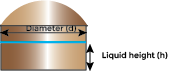
\includegraphics[scale=1]{DigesterWOCDimensions_1}
\end{center}

{
$=\dfrac
	{
		12,000
		\dfrac
			{
			ft^3 \enspace sludge
			}
			{
			day
			}
		*7.48 \dfrac
				{
				gal
				}
				{
				ft^3
				}	
		*(8.34*0.045*0.70) 
		\dfrac
			{lbs VS}
			{gal \enspace  sludge}
	}
	{
		(	\dfrac
			{
			\pi
			}
			{
			4
			}
			*100^2*20
		)
		ft^3
	}
=\boxed
	{
		0.15 \dfrac
			{
			lbs \enspace VS
			}
			{
			day-ft^3
			}
	}
$}\\

\item How much gas is produced in the above digester in $ft^3$/day if the digested sludge contains 2.5\% total solids of which 59\% is volatile solids and the gas production rate is 14 $ft^3$/lb VS destroyed?\\
Solution:\\

{
$
Digester \enspace VS \enspace reduction (\%)=
	\dfrac
	{0.70 - .59}
	{0.70 - 0.70 *0.59}
	*100=38.3\%
$
}\\
\vspace{6mm}

{
$
	\dfrac
	{
	lbs \enspace VS \enspace reduction
	}
	{
	day
	}
	=
	\dfrac
	{
	3153 lbs \enspace VS \enspace feed
		*  0.383 \enspace VS \enspace reduction
	}
	{
	day
	}
 	=1,208
	\dfrac
	{
	lbs \enspace VS \enspace reduction
	}
	{
	day 
	}
$
}\\
\vspace{6mm}

{
$
	\dfrac 
	{
	ft^3 gas \enspace produced
	}
	{
	day
	}
	=
	1208 \dfrac
			{
			lbs \enspace VS \enspace reduced
			}
			{
			day
			}
			*
		\dfrac
		{
		14 ft^3 \enspace gas \enspace produced
		}
		{
		lb \enspace VS \enspace reduced
		}
		=16,912 \dfrac
				{
				ft^3 \enspace digester \enspace 					gas \enspace produced
				}
				{
				day
				}
$
} 
\item The sludge feed to a digester is 80,000 gal/day. The sludge contains 4.5\% total solids with 75\% volatile solids. If 50\% of VS are reduced in the digester: 



\begin{enumerate}
\item Find lbs VS destroyed per 1000 gal of digester capacity per day if the digester radius is 55 ft with an operating sludge level of 25 ft.(5 points)

\vspace{1cm}
Solution:\\
Digester Volume: 
$
{
		(\pi*55^2*25)ft^3 *7.48 \dfrac{gal}{ft^3}
	}=1,776,220 gallons=1,776.2 \enspace(1000 \enspace gallons)
$
\\
\vspace{3mm}
$
	\dfrac
	{
	lbs \enspace VS \enspace reduction
	}
	{
	day
	}
	=
	\dfrac
	{
	80,000 gal * 8.34 \dfrac{lbs}{gal}*(0.045*0.75) \dfrac{lbs VS}{lb}*0.5\dfrac{lbs \enspace VS \enspace  reduction}{lb \enspace VS}
	}
	{
	day
	}$\\
\vspace{0.25cm}
$
 	=11,259
	\dfrac
	{
	lbs \enspace VS \enspace reduction
	}
	{
	day 
	}
$
\\
\vspace{3mm}


$
	\dfrac
	{
	lbs \enspace VS \enspace reduction
	}
	{
	1000 \enspace digester \enspace capacity
	}
	=
	\dfrac
	{
	11,259 \dfrac
			{
			lbs \enspace VS \enspace reduction
			}
			{
			day
			}
	}
	{	
	1,776.2 \enspace (1000 \enspace gallons)
	}
 	=\boxed{6.3
	\dfrac
	{
	lbs \enspace VS \enspace reduction
	}
	{
	1000 gallons \enspace digester \enspace volume 
	}}
$
\\

\vspace{1cm}

\item  What is the digester gas production in Btu/day? Assume 14 cu. ft digester gas per lb of VS destroyed and a 650 Btu/cu. ft heating value for the digester gas produced (5 points)
\end{enumerate}
\vspace{1cm}
Solution:\\

$
	\dfrac 
	{
	ft^3 gas \enspace produced
	}
	{
	day
	}
	=
	11,259 \dfrac
			{
			lbs \enspace VS \enspace reduced
			}
			{
			day
			}
			*
		\dfrac
		{
		14 ft^3 \enspace gas \enspace produced
		}
		{
		lb \enspace VS \enspace reduced
		}
		=157,626 \dfrac
				{
				ft^3 \enspace digester \enspace 					gas \enspace produced
				}
				{
				day
				}
$
\\
\vspace{1cm}


$
	\dfrac 
	{
	BTU \enspace produced
	}
	{
	day
	}
	=
	157,626 \dfrac
			{
			ft^3 \enspace gas \enspace produced
			}
			{
			day
			}
			*
		\dfrac
		{
		650 BTU \enspace gas \enspace produced
		}
		{
		ft^3 gas
		}
		=\boxed{102,456,900 \dfrac
				{
				BTU \enspace produced
				}
				{
				day
				}}
$

\item Two sludges are blended together as follows: 15,000 gal. primary sludge at 4.1\% solids. 28,000 gal. secondary sludge at 1.3\% solids. What is the combined solids concentration?  If the primary sludge is 68\% VS and the secondary sludge is 63\% VS, what is the VS concentration (\%) in the combined sludge?

Solution:

Combined solids concentration:
$
C_1*V_1 + C_2*V_2 = C_3*V_3$\\
$\implies C_3 = \dfrac{C_1*V_1 + C_2*V_2}{V3}=\dfrac{C_1*V_1 + C_2*V_2}{V_1 + V_2}=\dfrac{4.1*15,000 + 1.3*28,000}{15,000 + 28,000}=\boxed{2.28\%}
$\\
Lbs of VS in combined sludge:
$
C\textsubscript{VS1}*V_1 + C\textsubscript{VS2}*V_2 = C\textsubscript{VS3}*V_3$\\
$\implies C\textsubscript{VS3} = \dfrac{C\textsubscript{VS1}*V_1 + C\textsubscript{VS2}*V_2}{V3}=\dfrac{C\textsubscript{VS1}*V_1 + C\textsubscript{VS1}*V_2}{V_1 + V_2}$\\
$\implies C\textsubscript{VS3}
=\dfrac{4.1*15,000*0.68 + 1.3*28,000*0.63}{15,000 + 28,000}=\boxed{1.50\%}$
\\

\pagebreak
	
\item 10,000 gallons of sludge is pumped to an anaerobic digester/day at 4\% solids (70\% VS).  50\% of the VS are destroyed, creating 15 $ft^3$ of gas per lbs. of VS destroyed. How much gas is produced each day?\\

{
$
	\dfrac
	{
	lbs \enspace VS \enspace reduction
	}
	{
	day
	}
	=
	\dfrac
	{
	10,000 gal * 8.34 \dfrac{lbs}{gal}*(0.04*0.7) \dfrac{lbs VS}{lb}*\dfrac{0.5 lbs \enspace VS \enspace  reduction}{lb \enspace VS}
	}
	{
	day
	}
 	=1,168
	\dfrac
	{
	lbs \enspace VS \enspace reduction
	}
	{
	day 
	}
$
}\\
\vspace{3mm}

{
$
	\dfrac 
	{
	ft^3 gas \enspace produced
	}
	{
	day
	}
	=
	1,168 \dfrac
			{
			lbs \enspace VS \enspace reduced
			}
			{
			day
			}
			*
		\dfrac
		{
		15 ft^3 \enspace gas \enspace produced
		}
		{
		lb \enspace VS \enspace reduced
		}
		=17,520 \dfrac
				{
				ft^3 \enspace digester \enspace 					gas \enspace produced
				}
				{
				day
				}
$
} 

\item Two sludges are blended together as follows: 60,000 gal per day. primary sludge at 4.5\% solids and 28,000 gal secondary sludge at 5\% solids. 
\begin{enumerate}
\item What is the combined solids concentration?  (3 points)\\

$\dfrac{60,000*4.5+28,000*5}{88,000}=\boxed{4.66\%}$\\
\vspace{2cm}
\item How many lbs of solids (per day) are in the combined sludge (3 points)\\

$88,000 gal*8.34*0.0466 = \boxed{34,200 lbs}$\\
\vspace{2cm}


\item If the primary sludge is 68\% VS and the secondary sludge is 83\% VS, how many pounds of VS are in the combined sludge? (3 points)\\
$60,000 gal *\dfrac{8.34*0.045*0.68lbs \enspace VS}{gal}+28,000 gal *\dfrac{8.34*0.05*0.83lbs \enspace VS}{gal}=\boxed{25,003 lbs \enspace VS}$
\vspace{2cm}

\item What is the digester feed VS\%?  (3 points)\\
$\dfrac{25,003 lbs \enspace VS}{34,200 lbs TS}=\boxed{73.1\%}$

\vspace{2cm}



\item If the digester is 120’ diameter with a liquid height of 20’, what is the VS loading in lbs VS/ft3-day (3 points)\\

$\dfrac{25,003 lbs \enspace VS}{0.785*120^2*20}=\boxed{\dfrac{0.11 lbs \enspace VS}{day-ft^3}}$\\
\vspace{2cm}





\item If the digested sludge has 52\% VS, calculate the digester VS reduction percent (3 points)\\

$
Digester \enspace VS \enspace reduction (\%)=
	\dfrac
	{0.731 - .52}
	{0.731 - 0.731 *0.52}
	*100=\boxed{60.1\%}
$\\
\vspace{2cm}

\item What is the gas production (ft$^3$/day) if the digester produces 14 ft$^3$ gas/lb VS destroyed (3 points)\\
25,003*0.601$\dfrac{lbs\enspace VS destroyed}{}*\dfrac{14ft^3 \enspace gas \enspace produced}{lb \enspace VS \enspace destroyed}=\boxed{210,375ft^3 gas}$
\\
\vspace{2cm}

\item How many belt presses are needed to keep up with the digested sludge flow if the belt presses can be operated at a maximum flow of 50 GPM (3 points)\\

88,000$\dfrac{gal \enspace sludge}{day}*\dfrac{day}{1440min}=61 GPM$\\
@50 GPM per press - $\boxed{2 \enspace BFP \enspace required}$
\vspace{2cm}
\item If the digested sludge feed to the belt filter presses is 2.6\% and assuming the belt press feed solids capture is 90\%.  How many lbs of solids (dry) are produced by the BFP (4 points)\\
$88,000\dfrac{gal}{day}*8.34*0.026\dfrac{lbs \enspace solids \enspace feed}{day}*0.9\dfrac{lbs \enspace solids \enspace captured}{lbs \enspace solids \enspace feed}=\boxed{17,174 lbs \enspace solids \enspace per \enspace day}$
\vspace{2cm}

\item If the BFP produces a 20\% cake, how many wet tons cake produced per day (4 points)\\
$\dfrac{17,174 lbs \enspace solids \enspace produced}{day}*\dfrac{100 lbs \enspace cake}{20 lbs \enspace solids \enspace produced}*\dfrac{tons}{2,000 lbs}=\boxed{\dfrac{42.9tons}{day}}$
\vspace{2cm}

\item If the cake density is 68 lbs/cu. ft, how much time will it take to fill a 30 cu. yd bin (3 points)\\
(Ans. 15.4 hours)
$\dfrac{(42.9*2000)lbs \enspace cake}{day}*\dfrac{day}{1440 min}=\dfrac{59.583}{lbs \enspace cake}{min}$\\
$\dfrac{59.583}{lbs \enspace cake}{min}*\dfrac{ft^3}{68 lbs \enspace cake}=\dfrac{0.876ft^3}{min}$\\
$30yd^3*\dfrac{27ft^3}{yd^3}*\dfrac{min}{0.876ft^3}*\dfrac{hrs}{60 min}=\boxed{15.4hrs}$
\vspace{2cm}
\item What will be the cost of hauling dewatered cake per day @ \$65 per ton cake (2 points)\\
42.9$\dfrac{tons}{day}*\dfrac{\$65}{ton}=\boxed{\dfrac{\$2,789}{day}}$ 
\end{enumerate}

\item Calculate the VS loading to the digester in lbs/day if 25,000 gallons of sludge containing 4.5\% TS with and average VS content of 76\% is fed to the digester 

Solution:\\
$\dfrac{25,000 \enspace Gal}{day}*\dfrac{8.34 \enspace lbs \enspace sludge}{Gal}* \dfrac{(0.045*0.76) \enspace lbs \enspace VS \enspace feed}{lb \enspace sludge}=\boxed{\dfrac{7,131 \enspace lbs \enspace VS }{day} } $

\item Calculate the organic loading rate to two 320,000 gallon anaerobic digesters given:
Primary sludge feed rate of 25,000 gallons with 6.2\% TS containing 73\% solids and SG of 1.03.
Secondary sludge feed rate of 30,500 gallons with 3.8\% TS containing 77\% solids (7 points)
(Answer: 0.2lbs VS/day-ft3 ) 

\item 10,000 gallons/day of sludge is pumped to an anaerobic digester/day at 4\% solids (70\% VS).  If 50\% of the VS is destroyed, how many lbs of VS is destroyed per day?\\
Solution:\\
$\dfrac{10,000 \enspace Gal}{day}*\dfrac{8.34 \enspace lbs \enspace sludge}{Gal} \dfrac{0.04*0.7 \enspace lbs \enspace VS \enspace feed}{lb \enspace sludge}*\dfrac{0.5 \enspace lbs \enspace VS \enspace destroyed}{lbs \enspace VS \enspace feed}=\boxed{\dfrac{1,168lbs \enspace VS \enspace destroyed}{day} } $

\item  Two sludges are blended together as follows: 8,000 cu. ft primary sludge at 4.90\% solids and 23,000 gal. secondary sludge at 5.20\% solids. What is the combined solids concentration?\\


a. 3.84 \\
b. 6.23 \\
c. 5.12 \\
*d. 4.98 \\

\item  Calculate the VS loading to the digester in lbs/day if 10,000 cu. ft of sludge containing 4.8\% TS with and an average VS content of 82\% (Ans: 24,554)\\

\item  Calculate the VS loading to the digester in lbs/day if 25,000 gallons of sludge containing 4.5\% TS with and average VS content of 76\% is fed to the digester (Ans: 7,131)\\

\item  Calculate the \% VS reduction in a digester given the volatile solids content of the feed sludge to the digester is 76\% and the volatile solids content of the sludge leaving the digester is 55\% (Ans: 61.4)\\

\item  If an anaerobic digester receives sludge with VS of 76\% and discharges digested sludge with a 56\% VS.  Its VS reduction is:\\

a. 36\% \\
b. 48\% \\
*c. 60\% \\
d. 89\% \\

\item  Calculate the VS loading to the digester in lbs/day if 25,000 gallons of sludge containing 4.5\% TS with and average VS content of 76\% is fed to the digester \\

Correct Answer(s):
a. 7131.0 \\

\item  Calculate the organic loading rate to two 320,000 gallon anaerobic digesters given:
Primary sludge feed rate of 25,000 gallons with 6.2\% TS containing 73\% solids and SG of 1.03.
Secondary sludge feed rate of 30,500 gallons with 3.8\% TS containing 77\% solids (7 points)
(Answer: 0.2lbs VS/day-ft3 ) \\

Correct Answer(s): \\


\item  Calculate the VS loading to the digester in lbs/day if 25,000 gallons of sludge containing 4.5\% TS with and average VS content of 76\% is fed to the digester \\

*a. 7,131 lbs/day \\
b. 17,432 lbs/day \\
c. 19,256 lbs/day \\
d. 26,244 lbs/day \\

\item  What is the digester efficiency if the volatile solids concentration entering an anaerobic digester is 70\% and the volatile solids concentration leaving the digester is 50\%? \\

*a. 29\% \\
b. 40\% \\
c. 57\% \\
d. 71\% \\

\item  You are operating a 1 MGD trickling filter plant with a single stage anaerobic digester You pump about 3,000 gpd of sludge to the fixed cover digester.  The supernatant has a BOD of 950 mg/l The BOD loading coming from the supernatant in pounds per day is \\

a. 12 \\
*b. 24 \\
c. 36 \\
d. 48 \\

\item  How many pounds of solids are pumped to a digester each day, if the digester receives 10,000 gpd of sludge at 5\% density? \\

a. 417 lbs/day \\
b. 1,497 lbs/day \\
c. 2,337 lbs/day \\
d. 3,273 lbs/day \\
*e. 4,170 lbs/day \\

\item  If a digester loading is 0.05 lbs VSS/ft3/Day, how large must the digester be if it receives 1,000 lbs. of suspended solids per day with a volatile percentage of 75\%? \\

a. 3,750 cu.ft \\
b. 10,000 cu.ft \\
*c. 15,000 cu.ft \\
d. 26,666 cu.ft \\
e. 37,500 cu.ft \\

\item  What is the digester efficiency if the volatile solids concentration entering an anaerobic digester is 70\% and the volatile solids concentration leaving the digester is 50\%? \\

*a. 29\% \\
b. 40\% \\
c. 57\% \\
d. 71\% \\

\item  You are operating a 1 MGD trickling filter plant with a single stage anaerobic digester You pump about 3,000 gpd of sludge to the fixed cover digester.  The supernatant has a BOD of 950 mg/l The BOD loading coming from the supernatant in pounds per day is \\

a. 12 \\
*b. 24 \\
c. 36 \\
d. 48 \\

\item  How many pounds of solids are pumped to a digester each day, if the digester receives 10,000 gpd of sludge at 5\% density? \\

a. 417 lbs/day \\
b. 1,497 lbs/day \\
c. 2,337 lbs/day \\
d. 3,273 lbs/day \\
*e. 4,170 lbs/day \\


\item  If a digester loading is 0.05 lbs VSS/ft3/Day, how large must the digester be if it receives 1,000 lbs. of suspended solids per day with a volatile percentage of 75\%? \\

a. 3,750 cu.ft \\
b. 10,000 cu.ft \\
*c. 15,000 cu.ft \\
d. 26,666 cu.ft \\
e. 37,500 cu.ft \\

\end{enumerate}

\section*{Disinfection Math Problems}
\begin{enumerate}
\item What is the chlorine demand if the chlorine dosage is 15 mg/l and the residual is 3 mg/l?
Solution:\\
Chlorine dosage = chlorine demand + chlorine residual\\
$\implies chlorine \enspace demand = chlorine \enspace dosage - chlorine \enspace residual=15-3=\boxed{12mg/l}$
\vspace{0.25cm}
\item Calculate how many pounds per day of chlorine should be used to maintain a dosage of 12 mg/l at a 5.0 MGD flow.\\
Solution:\\
$lbs/day=conc. (mg/l)*flow(MGD)*8.34$\\
$lbs/day=12*5*8.34=\boxed{500.4lbs/day}$\\
\vspace{0.25cm}
\item If 80 pounds of chlorine are applied each day to a flow of 1.5 MGD, what is the dosage in mg/l?\\
\vspace{0.25cm}
Solution:\\
\vspace{0.25cm}
Applying the pounds formula:\\  $lbs/day=conc. (mg/l)*flow(MGD)*8.34$\\
\vspace{0.25cm}
$\implies conc. (mg/l)=\frac{lbs/day}{flow(MGD)*8.34}=\frac{80}{1.5*8.34}=\boxed{6.4mg/l}$
\vspace{0.25cm}
\item How many pounds per day of chlorine will be required to disinfect a secondary effluent flow of 1.68 MGD if the chlorine demand is found to be 8.5 mg/l and a residual of 3 mg/l is desired?\\
\vspace{0.25cm}
Chlorine dosage = chlorine demand + chlorine residual\\
\vspace{0.25cm}
$chlorine \enspace dosage=8.5+3=11.5mg/l$\\
$lbs/day=conc. (mg/l)*flow(MGD)*8.34=1.68*11.5*8.34=\boxed{161.2lbs/day}$\\
\vspace{0.25cm}
\item The chlorine demand is 4.8 mg/l and a chlorine residual is 0.75 mg/l is desired. For a flow of 2.8 MGD, how many pounds per day should the chlorinator be set to deliver.\\
Solution:\\
Chlorine dosage = chlorine demand + chlorine residual\\
\vspace{0.25cm}
$chlorine \enspace dosage=4.8+0.75=5.55mg/l$\\
\vspace{0.25cm}
To calculate pounds per day, applying the pounds formula:\\ 
\vspace{0.25cm}
$lbs/day=conc. (mg/l)*flow(MGD)*8.34=2.8*5.55*8.34=\boxed{129.6lbs/day}$\\
\vspace{0.25cm}
\item Chlorine is being fed at the rate of 75 pounds per day. Plant flow is 1.2 MGD. The chlorine residual is measured and found to be 2.6 mg/l Calculate chlorine demand.\\
a. 4.9 mg/l \\
b. 5.7 mg/l \\
c. 7.5 mg/l \\
d. 8.3 mg/l \\
\vspace{0.25cm}
Solution:\\
$Chlorine \enspace dosage (lbs/day)=conc. (mg/l)*flow(MGD)*8.34$\\
$\implies chlorine \enspace dosage \enspace conc. (mg/l)=\frac{lbs/day}{flow(MGD)*8.34}=\frac{75}{1.2*8.34}=7.5mg/l$\\
Chlorine dosage = chlorine demand + chlorine residual\\
\vspace{0.25cm}
$ \implies chlorine \enspace demand = chlorine \enspace dosage - chlorine \enspace residual=7.5-2.6=\boxed{4.9mg/l}$
\vspace{0.25cm}
\item Experience has shown that a minimum dosage of 24 mg/l is necessary in order to disinfect a wastewater effluent and leave a residual of 1.0 mg/l. How many pounds of chlorine must be fed at this dosage to a flow of 0.5 MGD?\\
Prior to sand filtration, a secondary effluent flow of 5 MGD
Solution:\\
Prior to sand filtration, a secondary effluent flow of 5 MGD
$Chlorine \enspace dosage (lbs/day)=conc. (mg/l)*flow(MGD)*8.34=24*0.5*8.34=\boxed{100lbs/day}$\\
\item 25 lbs/day of chlorine is being applied to a wastewater effluent flow of 250,000 gpd. Calculate the chlorine dosage in mg/l.\\
Solution:\\
$lbs/day=conc. (mg/l)*flow(MGD)*8.34$\\
$\implies conc. (mg/l)=\frac{lbs/day}{flow(MGD)*8.34}=\frac{25}{0.25*8.34}=\boxed{12mg/l}$
\item You wish to dose the influent channel at 5 mg/l chlorine to help control odors. The flow is 11.5 MGD.. How many pounds of chlorine must be fed each day? Is it necessary to maintain a chlorine residual to control odors?\\
Solution:\\
$lbs/day=conc. (mg/l)*flow(MGD)*8.34=5*11.5*8.34=\boxed{480lbs/day}$\\
No.  Chlorine residual is for disinfection only.  Odor control would not require a residual\\
\item Jar testing shows that the chlorine demand of an effluent is 12.5 mg/l. In order to assure disinfection, a residual of 1.0 mg/l is required. How many pounds of chlorine must be fed per 1MGD to assure disinfection?\\
Solution: 
$ chlorine \enspace dosage = chlorine \enspace demand \enspace + \enspace chlorine \enspace residual$\\
$\implies chlorine \enspace dosage = (12.5 \enspace + \enspace 1 )mg/l=13.5 mg/l$\\
$lbs/day=13.5(mg/l)*1(MGD)*8.34=\boxed{112.6 lbs/day}$
\item What is the chlorine dosage if the chlorinator is feeding 120 lbs/day and the average daily flow is 3.5 MGD?  What is the chlorine demand if the residual is 1.3 mg/l?\\
Solution:\\
a. $Chlorine \enspace dosage (lbs/day)=conc. (mg/l)*flow(MGD)*8.34$\\
$\implies chlorine \enspace dosage \enspace conc. (mg/l)=\frac{lbs/day}{flow(MGD)*8.34}=\frac{120}{3.5*8.34}=\boxed{4.1mg/l}$\\
b. Chlorine dosage = chlorine demand + chlorine residual\\
$ \implies chlorine \enspace demand = chlorine \enspace dosage - chlorine \enspace residual=4.1-1.3=\boxed{2.8mg/l}$

\item Experience has shown that a minimum dosage of 24 mg/l is necessary in order to disinfect a wastewater effluent and leave a residual of 1.0 mg/l. How many pounds of chlorine must be fed at this dosage to a flow of 0.5 MGD?\\
Solution:\\
$Chlorine \enspace dosage (lbs/day)=conc. (mg/l)*flow(MGD)*8.34=24*0.5*8.34=\boxed{100lbs/day}$\\
\vspace{0.25cm}
\item 25 lbs/day of chlorine is being applied to a wastewater effluent flow of 250,000 gpd. Calculate the chlorine dosage in mg/l.\\
Solution:\\
$lbs/day=conc. (mg/l)*flow(MGD)*8.34$\\
$\implies conc. (mg/l)=\frac{lbs/day}{flow(MGD)*8.34}=\frac{25}{0.25*8.34}=\boxed{12mg/l}$
\vspace{0.25cm}
\item You wish to dose the influent channel at 5 mg/l chlorine to help control odors. The flow is 11.5 MGD.. How many pounds of chlorine must be fed each day? Is it necessary to maintain a chlorine residual to control odors?\\
Solution:\\
$lbs/day=conc. (mg/l)*flow(MGD)*8.34=5*11.5*8.34=\boxed{480lbs/day}$\\
No.  Chlorine residual is for disinfection only.  Odor control would not require a residual\\
\item Jar testing shows that the chlorine demand of an effluent is 12.5 mg/l. In order to assure disinfection, a residual of 1.0 mg/l is required. How many pounds of chlorine must be fed per 1MGD to assure disinfection?\\
Solution: 
$ chlorine \enspace dosage = chlorine \enspace demand \enspace + \enspace chlorine \enspace residual$\\
$\implies chlorine \enspace dosage = (12.5 \enspace + \enspace 1 )mg/l=13.5 mg/l$\\
$lbs/day=13.5(mg/l)*1(MGD)*8.34=\boxed{112.6 lbs/day}$
\item What is the chlorine dosage if the chlorinator is feeding 120 lbs/day and the average daily flow is 3.5 MGD?  What is the chlorine demand if the residual is 1.3 mg/l?\\
\vspace{0.25cm}
Solution:\\
a. $Chlorine \enspace dosage (lbs/day)=conc. (mg/l)*flow(MGD)*8.34$\\
$\implies chlorine \enspace dosage \enspace conc. (mg/l)=\frac{lbs/day}{flow(MGD)*8.34}=\frac{120}{3.5*8.34}=\boxed{4.1mg/l}$\\
b. Chlorine dosage = chlorine demand + chlorine residual\\
$ \implies chlorine \enspace demand = chlorine \enspace dosage - chlorine \enspace residual=4.1-1.3=\boxed{2.8mg/l}$
\vspace{0.25cm}
\item A 2.5 MGD secondary flow is disinfected by the application of 320 lbs of chlorine per day.  This dose provides a chemical residual of 2.1 mg/l.  There is a need to switch to the use of sodium hypochlorite which has a 12.5\% available chlorine, SG of 1.2 and a cost of \$0.60 per gallon. Chlorine costs \$0.28/lb.\\ Calculate: 1) The chlorine demand, and 2) Cost difference (\$ per day) between chlorine and sodium hypochlorite\\
\vspace{0.25cm}
Dosage = Demand + Residual\\
\vspace{0.25cm}
\textbf{Dosage:}\\
\vspace{0.25cm}
$\dfrac{320 lbs \enspace chlorine}{day}=2.5 MGD * 8.34 * x \dfrac{mg}{l}$\\
\vspace{0.25cm}
$x \dfrac{mg}{l}=\dfrac{320}{2.5*8.34}=15.34\dfrac{mg}{l}$\\
\vspace{0.25cm}
Chlorine Demand = Dosage - Residual = 15.34 - 2.1 = $\boxed{13.24\dfrac{mg}{l}}$\\
\vspace{0.25cm}
Cost per day to use chlorine: $\dfrac{\$320}{lb}*\dfrac{\$0.28}{lb}=\$89.60$\\
\vspace{0.25cm}
To calculate the hypochlorite we need to determine the gallons per day of bleach required.\\
\vspace{0.25cm}
$320 \dfrac{lbs \enspace chlorine}{day}\enspace=\enspace x \dfrac{gal \enspace bleach}{day} \enspace * \enspace 8.34 * 1.2 \dfrac{lbs \enspace bleach}{per \enspace gal \enspace bleach}* \enspace 0.125 \dfrac{lbs \enspace chlorine}{lb \enspace bleach}$\\
\vspace{0.25cm}
$ \rightarrow x \dfrac{gal \enspace bleach}{day}\enspace = \enspace \dfrac{320}{8.34*1.2*0.125} \enspace = \enspace 256 \dfrac{gal \enspace bleach}{day}$\\
\vspace{0.25cm}
$\enspace 256 \dfrac{gal \enspace bleach}{day}*\dfrac{\$0.60}{gal \enspace bleach}=\$153.48$
\vspace{0.25cm}
Cost difference \$153.48 - \$89.60 = $\boxed{\$63.88}$
\vspace{0.25cm}
\item Three hundred pounds (300 lbs) per day of chlorine (cost = \$0.32/lb) are being used to  disinfect  a secondary  effluent flow of 6.5 MGD.  Due to  safety concerns, the substitution of sodium hypochlorite (12.5\% available chlorine, 10.0 lbs/gal and a cost of \$0.55/gal) for the chlorine  is being considered  at  this plant. What is the cost difference per day between the chlorine and sodium hypochlorite?\\
\vspace{0.25cm}
 (Ans:\$36/year)

\item The operator at a 1.5 MGD conventional activated sludge plant is considering using either HTH or sodium hypochlorite as an alternative to chlorine gas. Currently chlorine is being dosed at 15 mg/l in order to achieve a residual of 3.0 mg/l. Using the data provided below calculate the daily cost for chlorine, HTH, and sodium hypochlorite (NaOCl) (Sp.Gravity 1.21).
 
Chlorine $\rightarrow$ 0.15 \$/lb\\
HTH (70\% available chlorine) $\rightarrow$ 0.25 \$/lb\\
NaOCl (15\% available chlorine) $\rightarrow$ 0.35 \$/gal                                                        

\vspace{0.25cm}
\textbf{SOLUTION}\\
\textbf{lbs chlorine required:}\\
$\dfrac{1.5 MG}{day}*\dfrac{8.34lbs}{gallon}*\dfrac{15mg \enspace chlorine}{l}=\dfrac{188 lbs \enspace chlorine}{day}$\\
\vspace{0.25cm}
\textbf{Daily cost if chlorine is used:}\\
$188lbs \enspace chlorine*\dfrac{\$0.15}{lb \enspace chlorine}=\boxed{\$28.20}$\\
\vspace{0.25cm}
\textbf{Daily cost if HTH is used:}\\
$188lbs \enspace chlorine*\dfrac{lb \enspace HTH}{0.7lb \enspace chlorine}*\dfrac{\$0.25}{lb \enspace chlorine}=\boxed{\$67.14}$\\
\vspace{0.25cm}
\textbf{Daily cost if NaOCl is used:}\\
$188lbs \enspace chlorine*\dfrac{lb \enspace NaOCl}{0.15lb \enspace chlorine}*\dfrac{gal \enspace NaOCl}{8.34*1.21 lbs\enspace NaOCl}*\dfrac{\$0.35}{gal \enspace NaOCl}=\boxed{\$43.47}$
\pagebreak
\item A water storage tank is 30 feet in diameter and has a water depth of 18.5 feet. It is desired to super-chlorinate this tank with 30 ppm of chlorine, how many pounds of HTH will be required (HTH has 70\% available chlorine)?\\    
\vspace{0.25cm}
\textbf{Tank Volume:}\\
$0.785*30^2*18.5ft^3*7.48\dfrac{gal}{ft^3}=97,765 gal$\\
\vspace{0.25cm}
\textbf{lbs HTH required:}\\
$\dfrac{30lbs \enspace chlorine}{1,000,000lbs  \enspace water}*\dfrac{8.34lbs \enspace water}{gal \enspace water}*97,765 gal \enspace water *\dfrac{lb \enspace HTH}{0.70lb \enspace chlroine}=\boxed{35 lbs \enspace HTH}$
\vspace{0.25cm}
\item The chlorine demand is 4.8 mg/l and a chlorine residual is 0.75 mg/l is desired.  For a flow of 2.8 MGD, how many pounds per day should the chlorinator be set to deliver.\\
*a. 130 \\
b. 116 \\
c. 112 \\
d. 18 \\
e. 16 \\
\item Chlorine is being fed at the rate of 75 pounds per day. Plant flow is 1.2 MGD. The chlorine residual is measured and found to be 2.6 mg/l Calculate chlorine demand.\\
*a. 4.9 mg/l \\
b. 5.7 mg/l \\
c. 7.5 mg/l \\
d. 8.3 mg/l \\
\item Assuming that a chlorine residual of 0.5 mg/l is being maintained and the chlorine demand is 19.5 mg/l, approximately how many pounds of chlorine per day will be required to treat a flow of 5.0 MGD?\\
a. 21 lbs \\
b. 792 lbs \\
c. 813 lbs \\
*d. 834 lbs \\
\item Chlorine is being fed at the rate of 75 pounds per day. Plant flow is 1.2 MGD. The chlorine residual is measured and found to be 2.6 mg/l Calculate chlorine demand.\\
*a. 4.9 mg/l \\
b. 5.7 mg/l \\
c. 7.5 mg/l \\
d. 8.3 mg/l \\
\item If 25 Ibs/day of chlorine is being applied to a wastewater effluent flow of 250,000 gpd. Calculate the chlorine demand in mg/l if the chlorine residue is 1.2 mg/l.\\
a. 2.5 mg/l \\
*b. 10.8 mg/l \\
c. 15.1 mg/l \\
d. 6.3 mg/l \\
\item Calculate how many pounds per day of chlorine should be used to maintain a dosage of 12 mg/l at 6.0 MGD flow\\
a. 60 lbs/day \\
b. 450 lbs/day \\
c. 500 lbs/day \\
*d. 600 lbs/day \\
e. 6,700 lbs/day \\
\item Chlorine is being fed at the rate of 75 pounds per day. Plant flow is 1.2 MGD. The chlorine residual is measured and found to be 2.6 mg/l Calculate chlorine demand. \\
*a. 4.9 mg/l \\
b. 5.7 mg/l \\
c. 7.5 mg/l \\
d. 8.3 mg/l \\
\item Chlorine is being fed at the rate of 200 pounds per day. Plant flow is 4 MGD. The chlorine residual is measured and found to be 3 mg/l Calculate chlorine demand. \\
a. 3 mg/l \\
*b. 2 mg/l \\
c. 16 mg/l \\
d. 9 mg/l \\
\item The chlorine demand is 4.8 mg/l and a chlorine residual is 0.75 mg/l is desired.  For a flow of 2.8 MGD, how many pounds per day should the chlorinator be set to deliver. \\
*a. 130 \\
b. 116 \\
c. 112 \\
d. 18 \\
e. 16 \\
\item Chlorine is being fed at the rate of 75 pounds per day. Plant flow is 1.2 MGD. The chlorine residual is measured and found to be 2.6 mg/l Calculate chlorine demand. \\
*a. 4.9 mg/l \\
b. 5.7 mg/l \\
c. 7.5 mg/l \\
d. 8.3 mg/l \\
\item Assuming that a chlorine residual of 0.5 mg/l is being maintained and the chlorine demand is 19.5 mg/l, approximately how many pounds of chlorine per day will be required to treat a flow of 5.0 MGD? \\
a. 21 lbs \\
b. 792 lbs \\
c. 813 lbs \\
*d. 834 lbs \\
\item Chlorine is being fed at the rate of 75 pounds per day. Plant flow is 1.2 MGD. The chlorine residual is measured and found to be 2.6 mg/l Calculate chlorine demand. \\
*a. 4.9 mg/l \\
b. 5.7 mg/l \\
c. 7.5 mg/l \\
d. 8.3 mg/l \\
\item If 25 Ibs/day of chlorine is being applied to a wastewater effluent flow of 250,000 gpd. Calculate the chlorine demand in mg/l if the chlorine residue is 1.2 mg/l. \\
a. 2.5 mg/l \\
*b. 10.8 mg/l \\
c. 15.1 mg/l \\
d. 6.3 mg/l \\
\item Calculate how many pounds per day of chlorine should be used to maintain a dosage of 12 mg/l at 6.0 MGD flow \\
a. 60 lbs/day \\
b. 450 lbs/day \\
c. 500 lbs/day \\
*d. 600 lbs/day \\
e. 6,700 lbs/day \\
\item What is the chlorine residual of a 2.5 MGD secondary effluent stream if its chlorine demand is 9 mg/l and is treated with 300 lbs/day chlorine?   Ans:  5.4
\\
\item How many lbs per day of chlorine is required to maintain a dosage of 12 mg/l for a 5 MGD flow?   Ans:  500.4
\\
\item What is the chlorine residual of a 2.5 MGD secondary effluent stream if its chlorine demand is 9 mg/l and is treated with 300 lbs/day chlorine? Ans:  5.4
\\
\item How many lbs per day of chlorine is required to maintain a dosage of 12 mg/l for a 5 MGD flow?  Ans:  500.4
\\
\item What is the chlorine residual of a 2.5 MGD secondary effluent  Ans:  5.4
\\
\item How many lbs per day of chlorine is required to maintain a dosage of 12 mg/l for a 5 MGD flow? Ans:  500.4
\\
\item Experience has shown that a minimum dosage of 24 mg/l is necessary in order to disinfect a wastewater effluent and leave a residual of 1.0 mg/l. How many pounds of chlorine must be fed at this dosage to a flow of 0.5 MGD? Ans:  100.0
\\
\item 25 lbs/day of chlorine is being applied to a wastewater effluent ow of 250,000 gpd. Calculate the chlorine dosage in mg/l.  Ans:  12.0
\\
\item You wish to dose the in influent channel at 5 mg/l chlorine to help control odors. The flow is 11.5 MGD.  How many pounds of chlorine must be fed each day? Is it necessary to maintain a chlorine residual to control odors?   Ans:480.0\\
\item Jar testing shows that the chlorine demand of an effluent is 12.5 mg/l. In order to assure disinfection, a residual of 1.0 mg/l is required. How many pounds of chlorine must be fed per 1MGD to assure disinfection?  Ans:  112.6
\\
\item What is the chlorine dosage if the chlorinator is feeding 120 lbs/day and the average daily flow is 3.5 MGD?  Ans:  4.1 \\
\item What is the chlorine residual of a 2.5 MGD secondary effluent stream if its chlorine demand is 9 mg/l and is treated with 300 lbs/day chlorine?  Ans:  5.4
\\
\item How many lbs per day of chlorine is required to maintain a dosage of 12 mg/l for a 5 MGD flow?  Ans:  500.4
\\
\item Chlorine is being fed at the rate of 75 pounds per day. Plant flow is 1.2 MGD. The chlorine residual is measured and found to be 2.6 mg/l Calculate chlorine demand. \\
*a. 4.9 mg/l \\
b. 5.7 mg/l \\
c. 7.5 mg/l \\
d. 8.3 mg/l \\
\item Chlorine is being fed at the rate of 75 pounds per day. Plant flow is 1.2 MGD. The chlorine residual is measured and found to be 2.6 mg/l Calculate chlorine demand. \\
*a. 4.9 mg/l \\
b. 5.7 mg/l \\
c. 7.5 mg/l \\
d. 8.3 mg/l \\
\item Chlorine is being fed at the rate of 200 pounds per day. Plant flow is 4 MGD. The chlorine residual is measured and found to be 3 mg/l Calculate chlorine demand. \\
a. 3 mg/l \\
*b. 2 mg/l \\
c. 16 mg/l \\
d. 9 mg/l \\
\item Chlorine is being fed at the rate of 200 pounds per day. Plant flow is 4 MGD. The chlorine residual is measured and found to be 3 mg/l Calculate chlorine demand. \\
a. 3 mg/l \\
*b. 2 mg/l \\
c. 16 mg/l \\
d. 9 mg/l \\
\item The chlorine demand is 4.8 mg/l and a chlorine residual is 0.75 mg/l is desired.  For a flow of 2.8 MGD, how many pounds per day should the chlorinator be set to deliver. \\
*a. 130 \\
b. 116 \\
c. 112 \\
d. 18 \\
e. 16 \\
\item Chlorine is being fed at the rate of 75 pounds per day. Plant flow is 1.2 MGD. The chlorine residual is measured and found to be 2.6 mg/l Calculate chlorine demand. \\
*a. 4.9 mg/l \\
b. 5.7 mg/l \\
c. 7.5 mg/l \\
d. 8.3 mg/l \\
\item Assuming that a chlorine residual of 0.5 mg/l is being maintained and the chlorine demand is 19.5 mg/l, approximately how many pounds of chlorine per day will be required to treat a flow of 5.0 MGD? \\
a. 21 lbs \\
b. 792 lbs \\
c. 813 lbs \\
*d. 834 lbs \\
\item Chlorine is being fed at the rate of 75 pounds per day. Plant flow is 1.2 MGD. The chlorine residual is measured and found to be 2.6 mg/l Calculate chlorine demand. \\
*a. 4.9 mg/l \\
b. 5.7 mg/l \\
c. 7.5 mg/l \\
d. 8.3 mg/l \\
\item If 25 Ibs/day of chlorine is being applied to a wastewater effluent flow of 250,000 gpd. Calculate the chlorine demand in mg/l if the chlorine residue is 1.2 mg/l. \\
a. 2.5 mg/l \\
*b. 10.8 mg/l \\
c. 15.1 mg/l \\
d. 6.3 mg/l \\
\item Calculate how many pounds per day of chlorine should be used to maintain a dosage of 12 mg/l at 6.0 MGD flow \\
a. 60 lbs/day \\
b. 450 lbs/day \\
c. 500 lbs/day \\
*d. 600 lbs/day \\
e. 6,700 lbs/day \\
\item How many pounds of chlorine will be used in one day if the flow is 700,000 gpd and a uniform dose of 12 mg/l is applied? \\
*a. 7 lbs \\
b. 15 lbs \\
c. 22 lbs \\
d. 26 lbs \\
\item Assuming that a chlorine residual of 0.5 mg/l is being maintained and the chlorine demand is 19.5 mg/l, approximately how many pounds of chlorine per day will be required to treat a flow of 50 MGD? \\
a. 21 lbs \\
b. 792 lbs \\
c. 813 lbs \\
*d. 834 lbs \\
\item How many pounds of chlorine gas is necessary to treat 4,000,000 gallons of wastewater at a dosage of 2 mg/l? \\
a. 61 lbs \\
b. 65 lbs \\
*c. 67 lbs \\
d. 69 lbs \\
\item If you need a chlorine residual of 1 mg/l , how many pounds of chlorine must be applied each day if the fl ow is 2.5 MGD and the chlorine demand is l5 mg/l? \\
a. 291 .pounds/day \\
b. 312 pounds/day \\
*c. 334 pounds/day \\
d. 419 pounds/day \\
e. 516 pounds/day \\
\item Chlorine is being fed at the rate of 75 pounds per day. Plant flow is 1.2 MGD. The chlorine residual is measured and found to be 2.6 mg/l Calculate chlorine demand. \\
*a. 4.9 mg/l \\
b. 5.7 mg/l \\
c. 7.5 mg/l \\
d. 8.3 mg/l \\
\item Chlorine is being fed at the rate of 200 pounds per day. Plant flow is 4 MGD. The chlorine residual is measured and found to be 3 mg/l Calculate chlorine demand. \\
a. 3 mg/l \\
*b. 2 mg/l \\
c. 16 mg/l \\
d. 9 mg/l \\
\item The chlorine demand is 4.8 mg/l and a chlorine residual is 0.75 mg/l is desired.  For a flow of 2.8 MGD, how many pounds per day should the chlorinator be set to deliver. \\
*a. 130 \\
b. 116 \\
c. 112 \\
d. 18 \\
e. 16 \\
\item Chlorine is being fed at the rate of 75 pounds per day. Plant flow is 1.2 MGD. The chlorine residual is measured and found to be 2.6 mg/l Calculate chlorine demand. \\
*a. 4.9 mg/l \\
b. 5.7 mg/l \\
c. 7.5 mg/l \\
d. 8.3 mg/l \\
\item Assuming that a chlorine residual of 0.5 mg/l is being maintained and the chlorine demand is 19.5 mg/l, approximately how many pounds of chlorine per day will be required to treat a flow of 5.0 MGD? \\
a. 21 lbs \\
b. 792 lbs \\
c. 813 lbs \\
*d. 834 lbs \\
\item Chlorine is being fed at the rate of 75 pounds per day. Plant flow is 1.2 MGD. The chlorine residual is measured and found to be 2.6 mg/l Calculate chlorine demand. \\
*a. 4.9 mg/l \\
b. 5.7 mg/l \\
c. 7.5 mg/l \\
d. 8.3 mg/l \\
\item If 25 Ibs/day of chlorine is being applied to a wastewater effluent flow of 250,000 gpd. Calculate the chlorine demand in mg/l if the chlorine residue is 1.2 mg/l. \\
a. 2.5 mg/l \\
*b. 10.8 mg/l \\
c. 15.1 mg/l \\
d. 6.3 mg/l \\
\item Calculate how many pounds per day of chlorine should be used to maintain a dosage of 12 mg/l at 6.0 MGD flow \\
a. 60 lbs/day \\
b. 450 lbs/day \\
c. 500 lbs/day \\
*d. 600 lbs/day \\
e. 6,700 lbs/day \\
\end{enumerate}

\section*{Chemical Dosing Math Problems}

\begin{enumerate}

\item Polymer is being added at 0.2 mg/l in order to achieve a 98\% capture efficiency for a belt press.  The feed to the belt press is 75 gallons per minute, containing 2.5\% solids.  Given the polymer costs \$250 per gallon of 4.5\% active polymer with a specific gravity of 1.08.  What is the cost of polymer per dry ton of solids captured  \\
\vspace{0.25cm}
\textbf{Solution:}\\
\vspace{0.25cm}
\textbf{lbs polymer required:}\\
$75*1440 \dfrac{gal \enspace sludge}{day}* 8.34 \dfrac{lbs \enspace sludge}{gal \enspace sludge} *\dfrac{0.2lbs \enspace polymer}{1,000,000 lbs \enspace sludge}$\\
\vspace{0.25cm}
$= 0.1801 \dfrac{lbs \enspace polymer}{day}$\\

\vspace{0.25cm}
\textbf{gallons polymer solution required:}\\ $0.1801 \dfrac{lbs \enspace polmyer}{day}\enspace=\enspace x \dfrac{gal \enspace polymer \enspace solution}{day} \enspace * \enspace \dfrac{8.34*1.08lbs \enspace polymer \enspace solution}{\enspace gal \enspace polymer \enspace solution}* \enspace 0.045 \dfrac{lbs \enspace polymer}{lb \enspace polymer \enspace solution}$\\
\vspace{0.25cm}
=0.444$\dfrac{gal \enspace polymer \enspace solution}{day}$
\vspace{0.25cm}

\textbf{Polymer cost:}\\
$\dfrac{\$250}{gallon \enspace polymer \enspace soultion}*\dfrac{0.444 gal \enspace polymer \enspace soultion}{day}$\\
\vspace{0.25cm}
=$\dfrac{\$111}{day}$\\
\vspace{0.25cm}
\textbf{Dry tons of solids captured:}\\
$ 75*1440\dfrac{gal \enspace sludge}{day}*\dfrac{8.34*0.025\enspace lbs \enspace solids}{gal \enspace sludge}*\dfrac{0.98\enspace lbs \enspace solids \enspace captured}{lbs \enspace solids}*\dfrac{ton \enspace solids}{2000 lbs \enspace solids}$\\
=$\dfrac{11tons \enspace dry \enspace solids}{day}$\\
\vspace{0.25cm}
\textbf{Polymer cost per dry ton of solids captured:}\\
\vspace{0.25cm}
$\dfrac{\$111 per day}{11 tons \enspace dry \enspace solids \enspace per \enspace day}= \boxed{\$10.09}$

\vspace{0.25cm}
\item A 50 MGD flow is being treated with 20 mg/l ferric chloride.   How many lbs of ferric chloride is required daily \\
\vspace{0.3cm}
\textbf{lbs ferric chloride required:}\\
$\dfrac{50 MG}{day}*\dfrac{8.34lbs}{gallon}*\dfrac{20mg \enspace ferric \enspace chloride}{l}=\boxed{\dfrac{8,340 lbs \enspace ferric \enspace chloride}{day}}$\\
\vspace{0.25cm}
\item If the ferric chloride solution used contains 40\% dry ferric chloride with a specific gravity of 1.4, what is its required feed rate in GPM (7 points)\\
\vspace{0.25cm}
\textbf{Required $FeCl_3$ feed (gal/min) to feed 8,340 lbs ferric chloride:}\\
$\dfrac{8,340 lbs \enspace FeCl_3}{day}=\dfrac{x gal \enspace FeCl_3 \enspace soltn.}{minute}*\dfrac{8.34*1.4 lbs \enspace FeCl_3 \enspace soltn}{gal \enspace FeCl_3 \enspace soltn.}*\dfrac{0.4 lbs \enspace FeCl_3}{lbs \enspace FeCl_3 \enspace soltn.}*\dfrac{1440min}{day}$\\
$\implies x=\dfrac{8,340}{8.34*1.4*0.4*1440}=\boxed{\dfrac{1.24gal}{min}}$\\
\vspace{0.25cm}
\item What is the daily ferric chloride dosing cost if the ferric chloride cost is \$580/dry ton ferric chloride (5 points)\\
\textbf{Daily ferric chloride dosing cost:}\\
\vspace{0.25cm}
$\dfrac{8,340lbs \enspace FeCl_3}{day}*\dfrac{ton}{2000 lbs}*\dfrac{\$580}{ton \enspace FeCl_3}=\boxed{\dfrac{\$2,419}{day}}$
\vspace{0.25cm}
\item A 0.5\% (based on dry weight) solution of polymer is being fed to a secondary effluent prior to sand filtration. It is desired to dose this effluent at 2.5 mg/l. Assuming an effluent flow of 3000 gpm, at what rate (gpm)  should  the polymer feed pump be set?\\	·
\vspace{0.25cm}
\textbf{lbs polymer required:}\\
$\dfrac{3000 gallons}{min}*\dfrac{8.34 \enspace lbs \enspace effluent}{gallon}*\dfrac{2.5 \enspace lbs \enspace polymer}{1,000,000 lbs \enspace effluent}=\dfrac{0.0626 lbs \enspace polymer}{min}$\\
\vspace{0.25cm}
\textbf{Required pumping rate to feed 0.0626 lbs polymer minute:}\\
$\dfrac{0.0626 \enspace lbs \enspace polymer}{min}=\dfrac{x \enspace gallon \enspace polymer  \enspace solution}{minute}*\dfrac{8.34 \enspace lbs \enspace polymer \enspace solution}{gallon \enspace polymer \enspace solution}*\dfrac{0.005 \enspace lbs \enspace polymer}{lbs \enspace polymer \enspace solution}$\\
\vspace{0.25cm}
$\dfrac{x \enspace gallon \enspace polymer solution}{minute}=\dfrac{0.0626}{8.34*0.005}=\boxed{\dfrac{1.5 \enspace gallon}{min}}$\\
\vspace{0.25cm}
\item How many pounds of dry polymer should be added to how many gallons  of water  to make enough 2\% polymer  solution to dose a 10 MGD secondary  effluent flow at 3.0 ppm of polymer?\\
\vspace{0.25cm}
\textbf{lbs polymer required:}\\
$10 MGD*\dfrac{8.34lbs \enspace effluent}{gallon}*\dfrac{3mg \enspace polymer}{l}=\dfrac{250.2 lbs \enspace polymer}{day}$\\
\vspace{0.25cm}
\textbf{Required pumping rate to feed 250.2 lbs polymer minute:}\\
$\dfrac{250.2 lbs \enspace polymer}{day}=\dfrac{x gallon \enspace polymer \enspace solution}{day}*\dfrac{8.34 lbs \enspace polymer \enspace solution}{gallon \enspace polymer \enspace solution}*\dfrac{0.02 lbs \enspace polymer}{lbs \enspace ploymer \enspace solution}$\\

\vspace{0.25cm}
$\dfrac{x gallon \enspace polymer \enspace solution}{day}=\dfrac{250.2}{8.34*0.02}=\boxed{\dfrac{1500 gallon}{day}}$\\
\vspace{0.25cm}
\textbf{This can also be done as follows:}\\
$\dfrac{250.2 lbs \enspace polymer}{day}*\dfrac{lbs \enspace ploymer \enspace solution}{0.02 lbs \enspace polymer}*\dfrac{gallon \enspace polymer \enspace solution}{8.34 lbs \enspace polymer \enspace solution}=\boxed{\dfrac{1500 gallon}{day}}$\\
\vspace{0.25cm}
$\boxed{\textbf{So dissolve 250.2 lbs polymer in 1500 gallons}}$\\
\vspace{0.25cm}
\textbf{Check:}
$\dfrac{250.2lbs \enspace polymer}{1500*8.34 lbs \enspace polymer \enspace solution}=\dfrac{0.02 lbs \enspace polymer}{lb \enspace polymer \enspace solution}=2\% polymer$
\vspace{0.25cm}

\item A 0.35\% solution of polymer is being fed to a secondary effluent prior to sand filtration. The polymer feed pump is set to pump 0.5 gpm to an effluent flow of 4200 gpm. What is the polymer dose rate in ppm?\\
\vspace{0.25cm}
\textbf{Pounds polymer pumped:}\\
$\dfrac{0.5gal \enspace PS}{min}*\dfrac{8.34lbs \enspace PS}{gal \enspace PS}*\dfrac{0.0035lbs \enspace P}{lb \enspace PS}=\dfrac{0.0146lbs \enspace Polymer}{min}$\\
\textbf{Polymer dose rate:}\\
$\dfrac{lbs \enspace polymer}{10^6 \enspace lbs \enspace effluent}(ppm \enspace or \enspace \dfrac{mg}{l})=\dfrac{0.0146lbs \enspace min}{\dfrac{8.34*4,200}{1,000,000}10^6 \enspace lbs \enspace effluent}=\boxed{0.42 ppm \enspace polymer}$
\vspace{0.25cm}
\item Liquid alum (49\% alum, sp. gravity 1.32, \$1.85/gal)) is being used to remove phosphorus from a 600,000 gpd activated sludge effluent. Two hundred milligrams per liter (200 mg/l) of alum, $Al_2(S0_4)_3.14H_20$, is required to give adequate removal of the phosphorus in this effluent. Calculate the daily cost of liquid alum needed to remove phosphorus. [Formula Weights: Al =27, $Al_2(S0_4)_3.14H_20$ =594]\\
\vspace{0.25cm}
\textbf{lbs alum required:}\\
$\dfrac{0.6 MG}{day}*\dfrac{8.34lbs}{gallon}*\dfrac{200mg \enspace alum}{l}=\dfrac{1001 lbs \enspace alum}{day}$\\
\vspace{0.25cm}
\textbf{Required liquid alum feed (gal/day) to feed 1001 lbs alum:}\\
$\dfrac{1001 lbs \enspace alum}{day}=\dfrac{x gallon \enspace liquid \enspace alum}{minute}*\dfrac{8.34*1.32 lbs \enspace liquid \enspace alum}{gallon \enspace liquid \enspace alum}*\dfrac{0.49 lbs \enspace alum}{lbs \enspace liquid \enspace alum}$\\
\vspace{0.25cm}
$\implies x=\dfrac{1001}{8.34*1.32*0.49}=186gal$\\
\vspace{0.25cm}
\textbf{Daily cost of liquid alum to remove phosphorous:}\\
$\dfrac{186gal}{day}*\dfrac{\$1.85}{gal}=\boxed{\dfrac{\$344.10}{day}}$

\vspace{0.25cm}

\item A 1.5\% polymer solution (based on dry weight) is to be fed at the rate of 3.5 pp to a secondary effluent flow of 4.0 MGD.\\
(a) Calculate the polymer pump feed rate (gallon per minute) necessary to dose this secondary effluent. \\
(b) How many gallons per day of polymer solution will be required for an average flow of 3470 gpm?\\ 
\vspace{0.25cm}
(a)
\begin{itemize}
\item \textbf{Polymer required:}\\
$4*3.5*8.34=\dfrac{116.8 lbs \enspace polymer}{day}$\\
\item \textbf{Feed rate ($\dfrac{gal}{min}$):}\\
$\dfrac{116.8lbs \enspace polymer}{day}*
\dfrac{100lbs \enspace polymer \enspace solution}{1.5 lbs polymer}*
\dfrac{gal \enspace polymer \enspace solution}{8.34 lbs \enspace polymer \enspace solution}*
\dfrac{day}{1440min}=\boxed{0.65\dfrac{gal}{min}}$
\end{itemize}
\vspace{0.25cm}
(b)
\begin{itemize}

\item \textbf{Polymer required:}\\
$\bigg[\dfrac{3470gal}{min}*
\dfrac{MG}{1,000,000gal}*
\dfrac{1440min}{day}\bigg]MGD*3.5*8.34=\dfrac{145.9 lbs \enspace polymer}{day}$\\
\item \textbf{Feed rate ($\dfrac{gal}{min}$):}\\
$\dfrac{145.9lbs \enspace polymer}{day}*
\dfrac{100lbs \enspace polymer \enspace solution}{1.5 lbs polymer}*
\dfrac{gal \enspace polymer \enspace solution}{8.34 lbs \enspace polymer \enspace solution}*
\dfrac{day}{1440min}=\boxed{0.81\dfrac{gal}{min}}$
\end{itemize}
\vspace{0.25cm}

\item Liquid alum (Sp. gravity 1.32, 49\% Alum, \$1.70 per gallon,) is being used to remove phosphorus from a 595,000 gal/day secondary. A dose of 14.0 mg/l of aluminum is required to give adequate removal of the phosphorus in this effluent. Calculate the daily cost of liquid alum. (Note: Dry alum contains 9.4\% aluminum).\\
\vspace{0.25cm}
\textbf{Aluminum Required:}\\
$0.595*14*8.34=\dfrac{69.47 lbs \enspace aluminum}{day}$\\
\textbf{Cost of alum ($\dfrac{\$}{day}$):}\\
$\dfrac{69.47lbs \enspace aluminum}{day}*
\dfrac{100lbs \enspace alum}{9.4 lbs \enspace aluminum}*
\dfrac{100lbs \enspace alum \enspace solution}{49 lbs \enspace alum}*
\dfrac{gal \enspace alum \enspace solution}{(8.34*1.32) lbs \enspace alum \enspace solution}*
\dfrac{\$1.70}{gal \enspace alum \enspace solution}=\boxed{\dfrac{\$232.91}{day}}$
\vspace{0.25cm}

\item Polymer solution (0.5\% weight to weight) is being fed at the rate of 0.83 gpm to a secondary effluent flow of 1950 gpm prior to sand filtration. Calculate the polymer dose in units of ppm.\\
\vspace{0.25cm}
\textbf{Polymer Dose - $\dfrac{lbs \enspace polymer}{10^6 lbs \enspace effluent}$ which is $\dfrac{mg}{l}$ or ppm:\\
\vspace{0.25cm}
polymer solution(PS) \& polymer(P)}\\
$\dfrac{0.83gal \enspace PS}{min}*
\dfrac{8.34lbs \enspace PS}{gal \enspace PS}*
\dfrac{0.005lbs \enspace P}{lbs \enspace PS}*
\dfrac{min}{\dfrac{(8.34*1950)}{1,000,000}10^6 lbs \enspace effluent}=\boxed{\dfrac{2.13mg}{l} \enspace polymer}$

\vspace{0.25cm}

\item A 4.5\% (weight to weight basis) solution of polymer is being fed to a secondary effluent prior to sand filtration. It is desired to dose at 2.4 mg/l. Assuming an effluent flow of 6550 gpm, at what rate (gallons per minute) should the polymer feed pump be set?\\
\vspace{0.25cm}
\textbf{Polymer feed rate GPM:}\\
$6550*8.34*\dfrac{2.4}{10^6}\dfrac{lbs \enspace polymer}{min}*
\dfrac{100lbs \enspace polymer \enspace solution}{4.5 lbs polymer}*
\dfrac{gal \enspace polymer \enspace solution}{8.34 lbs \enspace polymer \enspace solution}=\boxed{0.35\dfrac{gal}{min}}$
\pagebreak
\item Polymer is being added at 0.3 mg/l in order to achieve a 92\% capture efficiency for a belt press. The feed to the belt press is 100 gallons per minute, containing 2.5\% solids. Given the polymer costs \$460 per gallon of 4\% active polymer with a specific gravity of 1.1. What is the cost of polymer per dry ton of solids captured \\

Solution:\\
\textbf{lbs polymer required:}\\
$100*1440 \dfrac{gal \enspace sludge}{day}* 8.34 \dfrac{lbs \enspace sludge}{gal \enspace sludge} *\dfrac{0.3lbs \enspace polymer}{1,000,000 lbs \enspace sludge}$\\
\vspace{0.25cm}
$= 0.36 \dfrac{lbs \enspace polymer}{day}$\\

\vspace{0.25cm}
\textbf{gallons polymer solution required:}\\ $0.36 \dfrac{lbs \enspace polmyer}{day}\enspace=\enspace x \dfrac{gal \enspace polymer \enspace solution}{day} \enspace * \enspace \dfrac{8.34*1.1lbs \enspace polymer \enspace solution}{\enspace gal \enspace polymer \enspace solution}* \enspace 0.04 \dfrac{lbs \enspace polymer}{lb \enspace polymer \enspace solution}$\\
\vspace{0.25cm}
=0.982$\dfrac{gal \enspace polymer \enspace solution}{day}$
\vspace{0.25cm}

\textbf{Polymer cost:}\\
$\dfrac{\$460}{gallon \enspace polymer \enspace soultion}*\dfrac{0.982 gal \enspace polymer \enspace soultion}{day}$\\
\vspace{0.25cm}
=$\dfrac{\$451.26}{day}$\\
\vspace{0.25cm}
\textbf{Dry tons of solids captured:}\\
$ 100*1440\dfrac{gal \enspace sludge}{day}*\dfrac{8.34*0.025\enspace lbs \enspace solids}{gal \enspace sludge}*\dfrac{0.92\enspace lbs \enspace solids \enspace captured}{lbs \enspace solids}*\dfrac{ton \enspace solids}{2000 lbs \enspace solids}$\\
=$\dfrac{13.81 tons \enspace dry \enspace solids}{day}$\\
\vspace{0.25cm}
\textbf{Polymer cost per dry ton of solids captured:}\\
\vspace{0.25cm}
$\dfrac{\$451.26 per day}{13.81 tons \enspace dry \enspace solids \enspace per \enspace day}= \boxed{\$32.67}$
\vspace{0.25cm}
\item A flow of 5 MGD is being treated with 9.8 mg/l aluminum using liquid alum of 48\% strength and SG of 1.32.  Alum has 19\% aluminum. If the liquid alum costs \$1.62 per gallon, what is the cost per day 
\\
\vspace{0.25cm}
\textbf{Solution:}\\
\vspace{0.25cm}
\textbf{lbs aluminum required:}\\
$5 MGD * 8.34 * 9.8 \dfrac{lbs \enspace aluminum}{day} = 408.7 \dfrac{lbs \enspace aluminum}{day}$\\
\vspace{0.25cm}
\textbf{Alum needed to meet this dosing need:}\\
\vspace{0.25cm}
$408.7 \dfrac{lbs \enspace aluminum}{day}\enspace=\enspace x \dfrac{gal \enspace liquid \enspace alum}{day} \enspace * \enspace 8.34 * 1.32 \dfrac{lbs \enspace liquid \enspace alum}{per \enspace gal \enspace liquid \enspace alum}* \enspace 0.48 \dfrac{lbs \enspace alum}{lb \enspace liquid \enspace alum} \enspace * \enspace 0.19 \dfrac{lbs \enspace aluminum}{lb \enspace alum}$\\
\vspace{0.25cm}
$ \implies x \dfrac{gal \enspace liquid \enspace alum}{day}\enspace = \enspace \dfrac{408.7}{8.34*1.32*0.48*0.19} \enspace = \enspace 407 \dfrac{gal \enspace liquid \enspace alum}{day}$\\
\vspace{0.25cm}
Cost per day=$407 \dfrac{gal \enspace liquid \enspace alum}{day}*\dfrac{\$1.62}{gal \enspace liquid \enspace alum}=\boxed{\$659.45}$
\vspace{0.25cm}
\item Prior to sand filtration, a secondary effluent flow of 5 MGD is dosed with 0.75\% strength polymer solution to achieve a dose of 1.5mg/l of polymer.  a) What is the lbs of dry polymer per day necessary to treat this effluent, and b) What is the required GPM feed of the 0.75\% polymer:\\
Solution:\\
Correct Answer:\\
a)  lbs of dry polymer required (lbs formula)=$5MGD*8.34*1.5=\boxed{62.55 \dfrac{lbs \enspace polymer}{day}}$\\
\vspace{0.25cm}
b) Flow rate of 0.75\% strength polymer = $62.55 \dfrac{lbs \enspace polymer}{day}=\dfrac{x \dfrac{gal}{min}*1440\dfrac{min}{day}}{1,000,000\dfrac{gal}{MG}}*8.34*7500$\\
$ \implies x \dfrac{gal}{min}=\dfrac{62.55*1,000,000}{1440*8.34*7,500}=\boxed{0.7GPM} - Correct \enspace Answer$\\
\vspace{0.3cm}
Incorrect Answer 1:\\
a)  lbs of dry polymer required (lbs formula)=$5MGD*8.34*1.5*0.75=\boxed{46.9 \dfrac{lbs \enspace polymer}{day}}$\\
\vspace{0.25cm}
b) Flow rate of 0.75\% strength polymer = $62.55 \dfrac{lbs \enspace polymer}{day}=\dfrac{x \dfrac{gal}{min}*1440\dfrac{min}{day}}{1,000,000\dfrac{gal}{MG}}*8.34*7500$\\
$ \implies x \dfrac{gal}{min}=\dfrac{46.9*1,000,000}{1440*8.34*7,500}=\boxed{0.5GPM} - Incorrect \enspace Answer \#1$\\
\vspace{0.3cm}
Incorrect Answer \#2:\\
$\boxed{62.6GPM} - Incorrect \enspace Answer \#2$\\
\vspace{0.3cm}
Incorrect Answer\#3:\\
$\boxed{12.6GPM} - Incorrect \enspace Answer \#3$

\item If a chemical costs \$30 per ton, how much will it cost per year to treat a flow of 15 MGD if the average dose is 18 mg/l?\\
Solution:\\
\textbf{Tons of chemical required per year:} (use lbs formula)\\ $\Big[15 \enspace MGD * 18 \enspace \dfrac{mg}{l}\enspace*8.34\Big]\dfrac{lbs}{day}* 365 \dfrac{days}{year}*\dfrac{ton}{2000lbs}=\enspace \dfrac{411 \enspace tons}{year}$

\textbf{Chemical cost:}\\
$\dfrac{411 \enspace tons}{year}*\dfrac{\$30}{ton}=\boxed{\$12,328 \enspace per \enspace year}$\\
\vspace{0.25cm}

\item Prior to sand filtration, a secondary effluent flow of 5 MGD is dosed with 0.75\% strength polymer solution to achieve a dose of 1.5mg/l of polymer. What is the required GPM feed of the 0.75% polymer: 

a. 12.6 GPM \\
b. 62.6 GPM \\
*c. 0.7 GPM \\
d. 0.5 GPM 





\end{enumerate}

\section*{Practice Problems - Pumping Power Requirements}
\begin{enumerate}
  \item If a pump is operating at 2,200 gpm and 60 feet of head, what is the water
horsepower? If the pump efficiency is 71\%, what is the brake horsepower?

\item The water horsepower of a pump is $10 \mathrm{Hp}$ and the brake horsepower output of the motor is $15.4 \mathrm{Hp}$. What is the efficiency of the pump?

\item The water horsepower of a pump is $25 \mathrm{Hp}$ and the brake horsepower output of the motor is $48 \mathrm{Hp}$. What is the efficiency of the pump?

\item The efficiency of a well pump is determined to be $75 \%$. The efficiency of the motor is estimated at $94 \%$. What is the efficiency of the well?

\item If a motor is $85 \%$ efficient and the output of the motor is determined to be 10
$\mathrm{BHp}$, what is the electrical horsepower requirement of the motor?

\item The water horsepower of a well with a submersible pump has been calculated at 8.2 WHp. The Output of the electric motor is measured as $10.3 \mathrm{BHp}$. What is the efficiency of the pump?

  \item Water is being pumped from a reservoir to a storage tank on a hill. The elevation difference between water levels is 1200 feet. Find the pump size required to fill the tank at a rate of 120 gpm. Express your answer in horsepower.

  \item A $25 \mathrm{hp}$ pump is used to dewater a lake. If the pump runs for 8 hours a day for 7 days a week, how much will it cost to run the pump for one week? Assume energy costs $\$ 0.07$ per kilowatt hour.

  \item A pump station is used to lift water 50 feet above the pump station to a storage tank. The pump rate is $500 \mathrm{gpm}$. If the pump has an efficiency of $85 \%$ and the motor has an efficiency of $90 \%$, find each of the following: Water Horsepower, Brake Horsepower, Motor Horsepower, and Wire-to-Water Efficiency.


  \item Find the brake horsepower for a pump given the following information: Total Dynamic Head $=75$ feet, Pump Rate $=150$ gpm, Pump Efficiency $=90 \%$, Motor Efficiency $=85 \%$

  \item Water is being pumped from a reservoir to a storage tank on a hill. The elevation difference between water levels is 1200 feet. Find the pump size required to fill the tank at a rate of 120 gpm. Express your answer in horsepower.

\end{enumerate}


\textbf{Solutions:}

\begin{enumerate}

\item  Solution:\\
\vspace{0.4cm}
water Hp = flow * head\\
$2,200GPM*60ft*\dfrac{Hp}{3,960 GPM-ft}=\boxed{Water \enspace Hp = 33.3Hp}$\\
\vspace{0.4cm}
pump Hp = brake Hp * pump efficiency\\
$brake \enspace Hp = \dfrac{33.3}{0.71}=\boxed{Brake \enspace Hp=47Hp}$
 \vspace{0.2cm}

 \item Solution:\\ 
 \vspace{0.2cm}
 \vspace{0.4cm}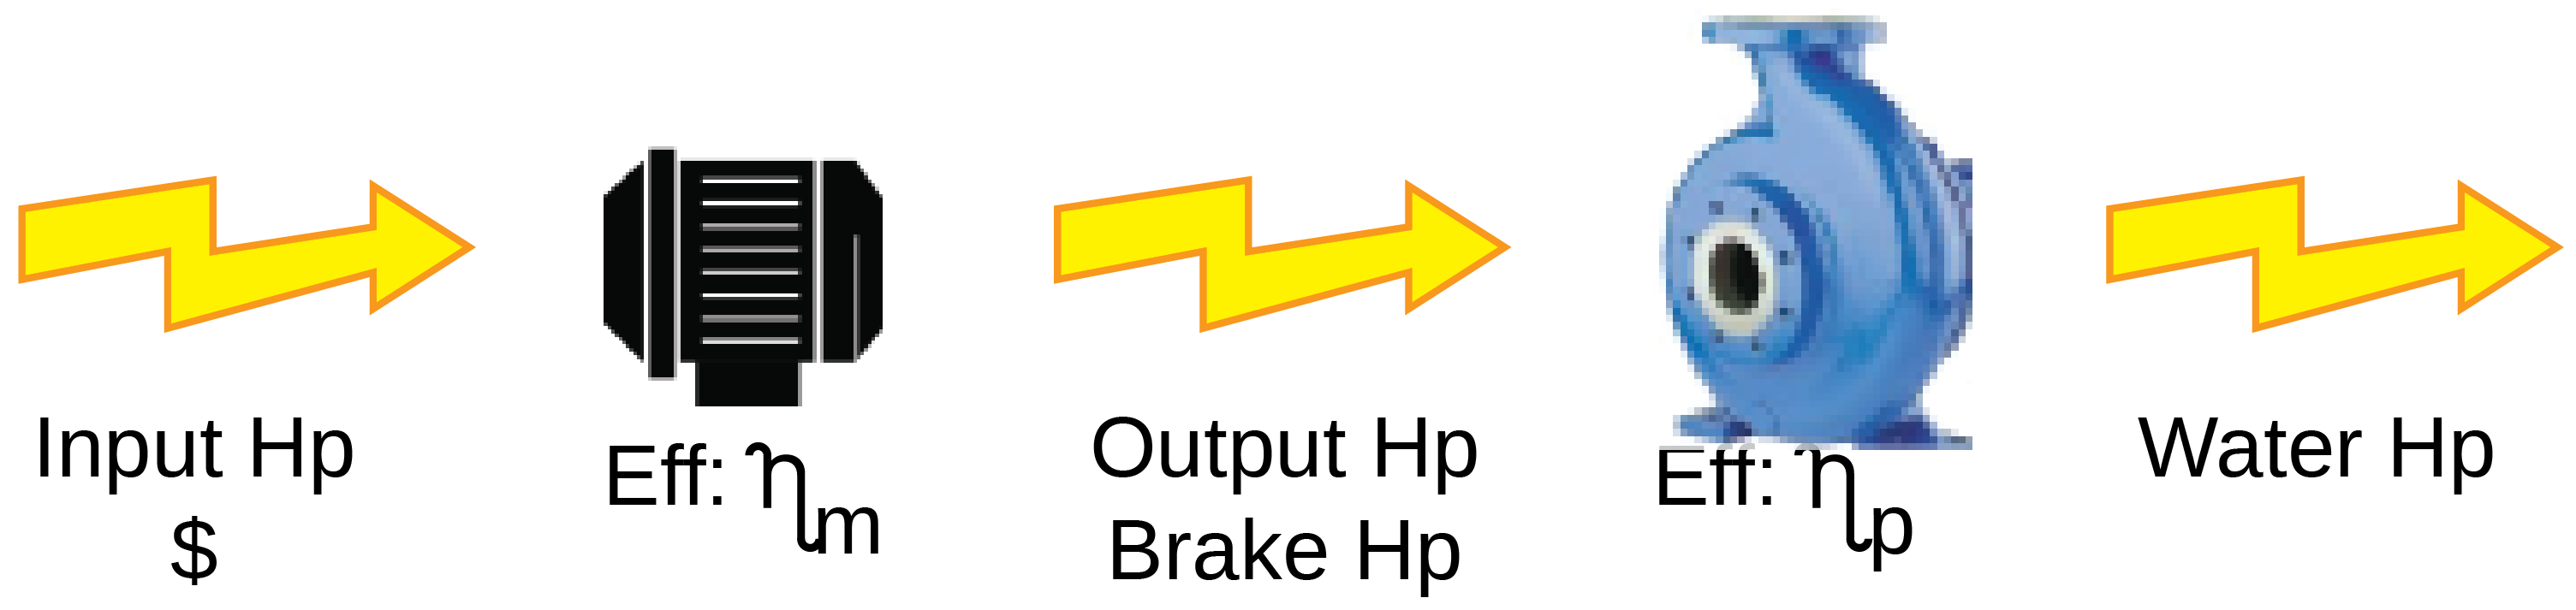
\includegraphics[scale=0.08]{PumpProblem}\\
 \vspace{0.2cm}
 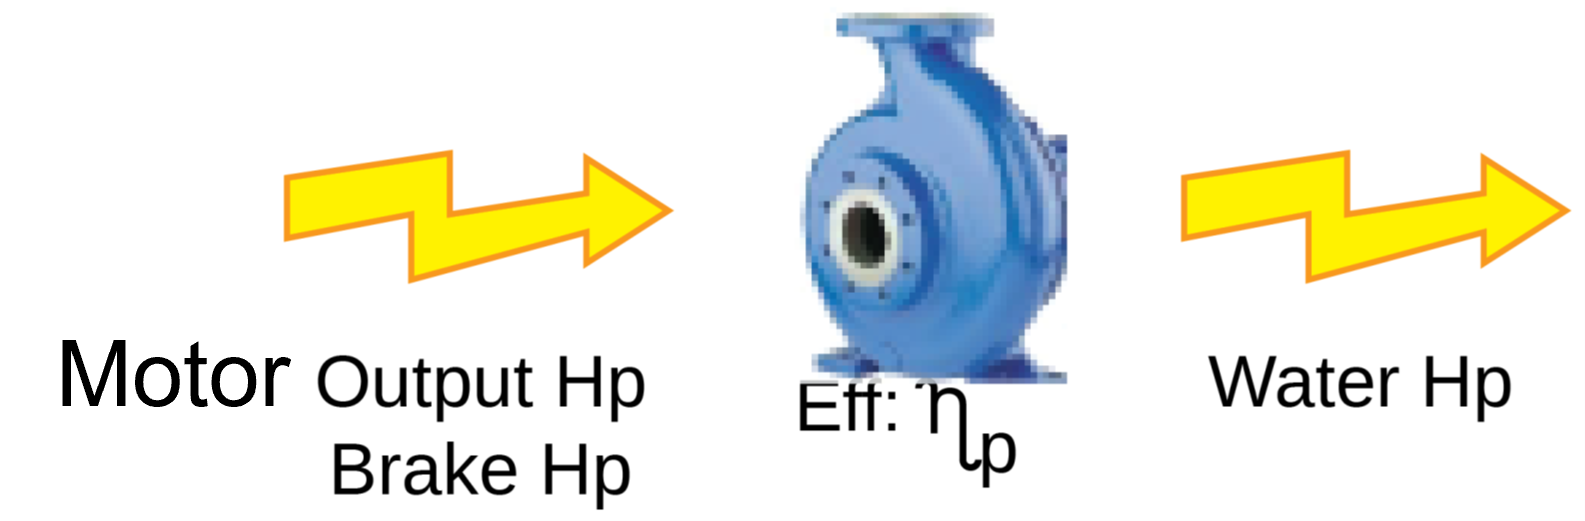
\includegraphics[scale=0.32]{PumpingProblemPump}
 $\eta_p=\dfrac{10 \mathrm{BHp}}{15.4 \mathrm{EHp}} \times 100=\boxed{65 \%}$
 \vspace{0.2cm}
 
 
 \item Solution:\\
  \vspace{0.2cm}
 \vspace{0.32cm}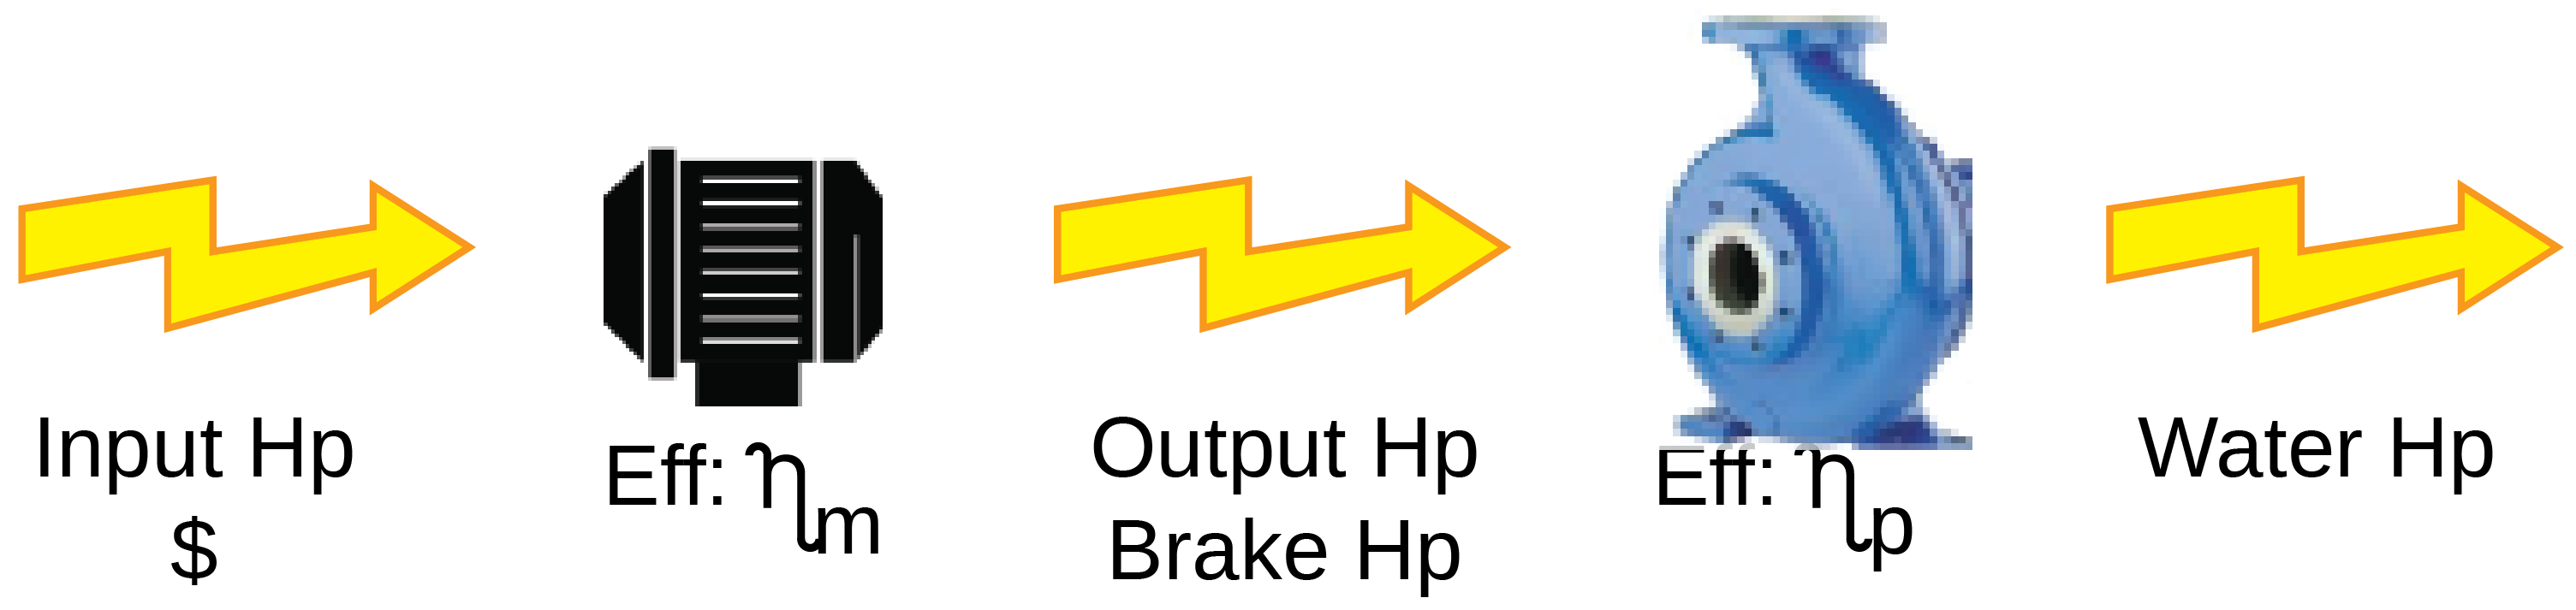
\includegraphics[scale=0.08]{PumpProblem}\\
 \vspace{0.2cm}
 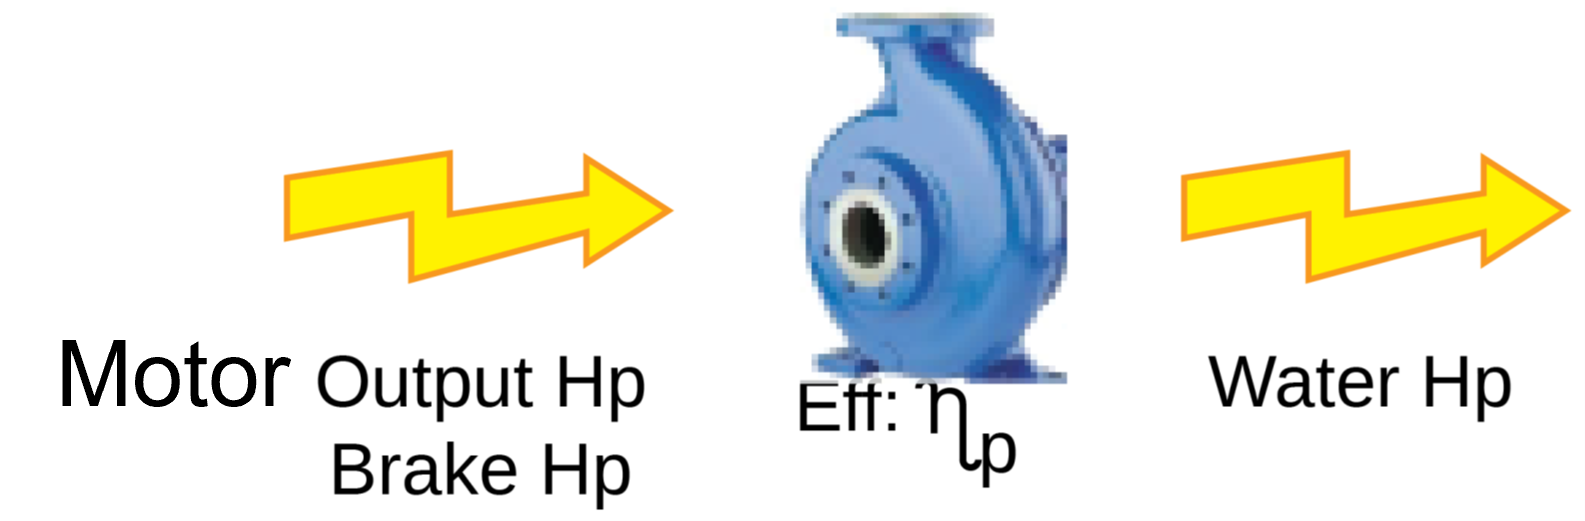
\includegraphics[scale=0.4]{PumpingProblemPump}
 \vspace{0.2cm}
$\eta_p=\dfrac{25 \mathrm{\enspace Water \enspace Hp}}{48 \mathrm{\enspace brake \enspace Hp}} \times 100=\boxed{52 \%}$
  \vspace{0.4cm}
 \item Solution:\\ 
 \vspace{0.2cm}
$Well \enspace efficiency=\eta_m * \eta_p \implies 0.94 \times 0.75=0.705 \times 100=\boxed{71 \%}$
 \vspace{0.2cm}


 \item Solution:\\
 \vspace{0.4cm}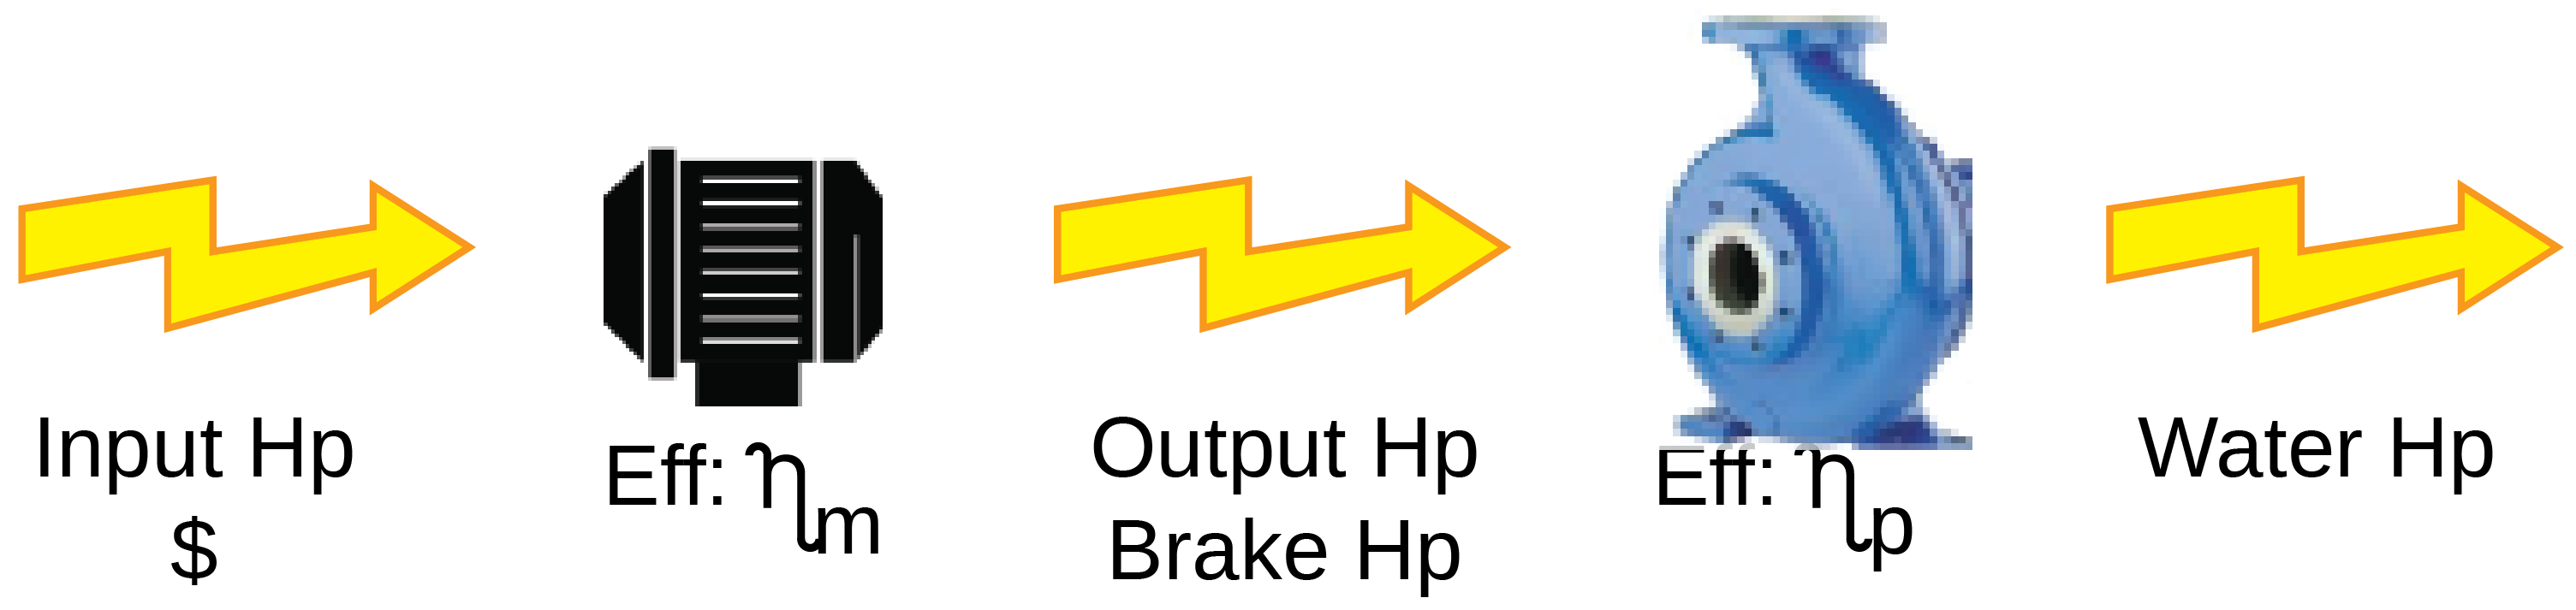
\includegraphics[scale=0.08]{PumpProblem}\\
 \vspace{0.2cm}
 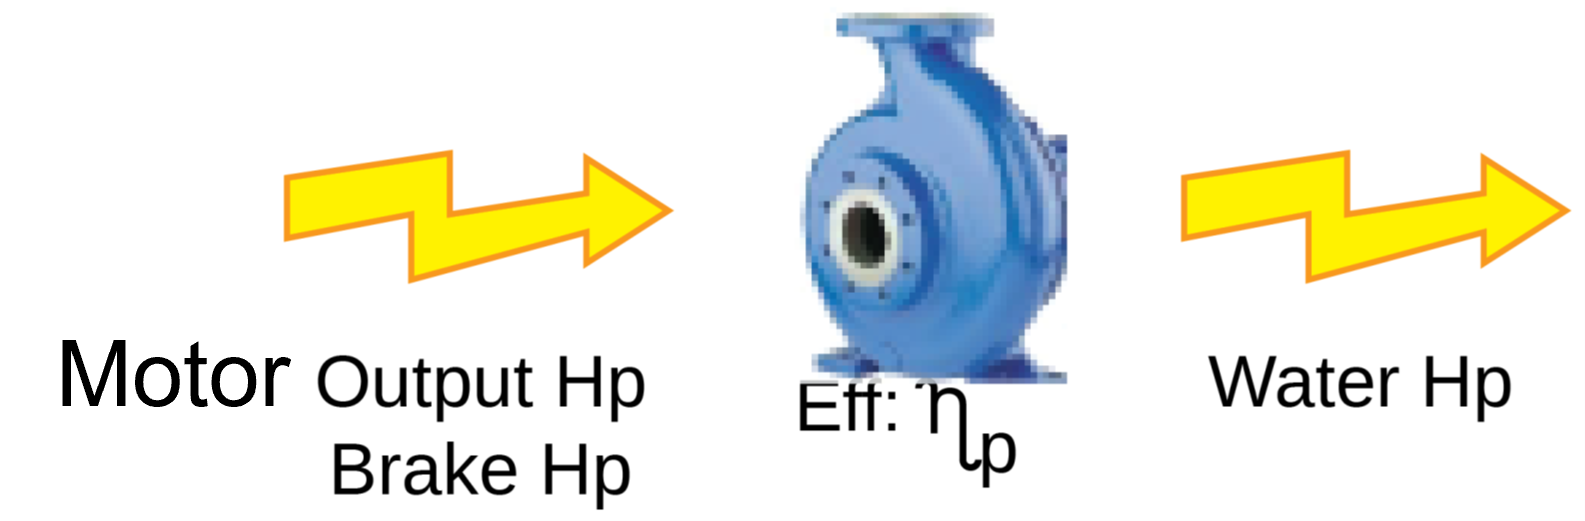
\includegraphics[scale=0.32]{PumpingProblemPump}
 \vspace{0.2cm}
$\dfrac{10 \mathrm{BHp}}{0.85}=\boxed{12 \mathrm{EHp \enspace or \enspace Input \enspace Hp}}$
 \vspace{0.4cm}


  \item Solution:\\ 
  \vspace{0.2cm}
 \vspace{0.08cm}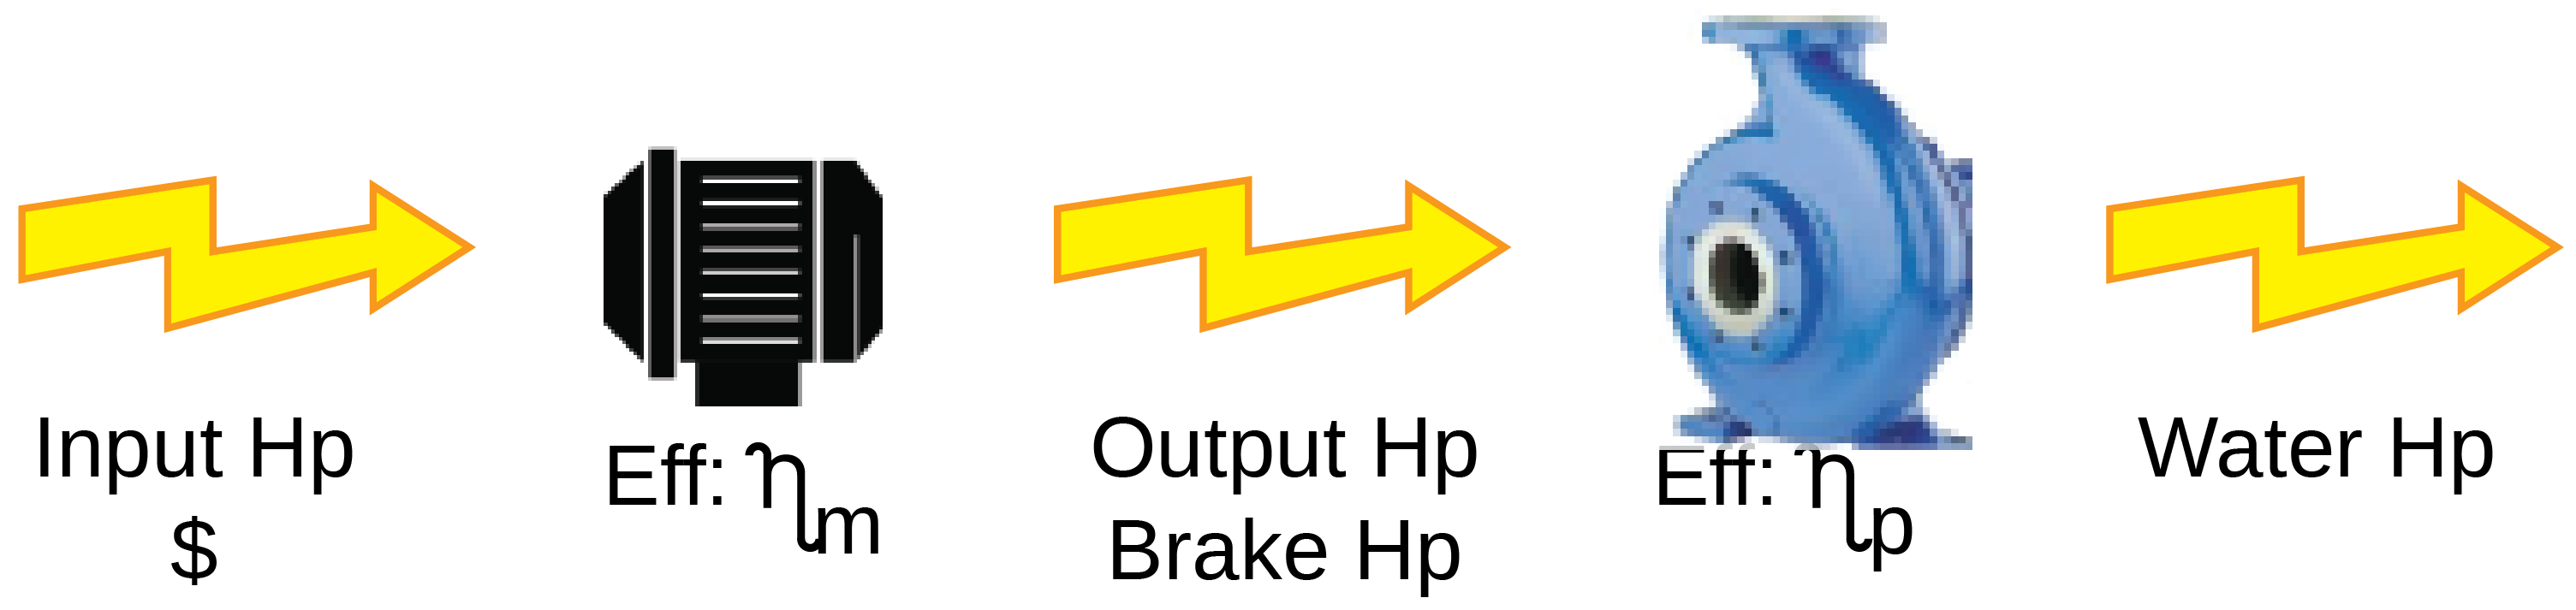
\includegraphics[scale=0.08]{PumpProblem}\\
 \vspace{0.2cm}
 \includegraphics[scale=0.32]{PumpingProblempump}
 \vspace{0.2cm}
$\eta_p=\dfrac{8.2 \mathrm{\enspace W \enspace Hp}}{10.3 \mathrm{\enspace BHp}} \times 100=\boxed{80 \%}$
 \vspace{0.2cm}


\item Solution:\\
\vspace{0.4cm}
water Hp = flow * head\\
\vspace{0.4cm}
$\mathrm{Water} \enspace \mathrm{Hp} = 120 \enspace \mathrm{gpm}*1,200 \enspace ft*\dfrac{\mathrm{Hp}}{3,960 \enspace \mathrm{gpm-ft}}=\boxed{ 37 \enspace \mathrm{Hp}}$\\
\vspace{0.2cm}


\item Solution:\\
\vspace{0.4cm}
$25 \enspace \mathrm{Hp}\dfrac{0.746 \enspace \mathrm{kW}}{\mathrm{Hp}}*\dfrac{8 \enspace \mathrm{hrs}}{\mathrm{day}}*\dfrac{7 \enspace \mathrm{days}}{\mathrm{month}}*\dfrac{\$0.07}{\mathrm{kWh}}=\boxed{\dfrac{\$73.1}{\mathrm{week}}}$\\
\vspace{0.2cm}

 \item Solution:\\
 \vspace{0.4cm}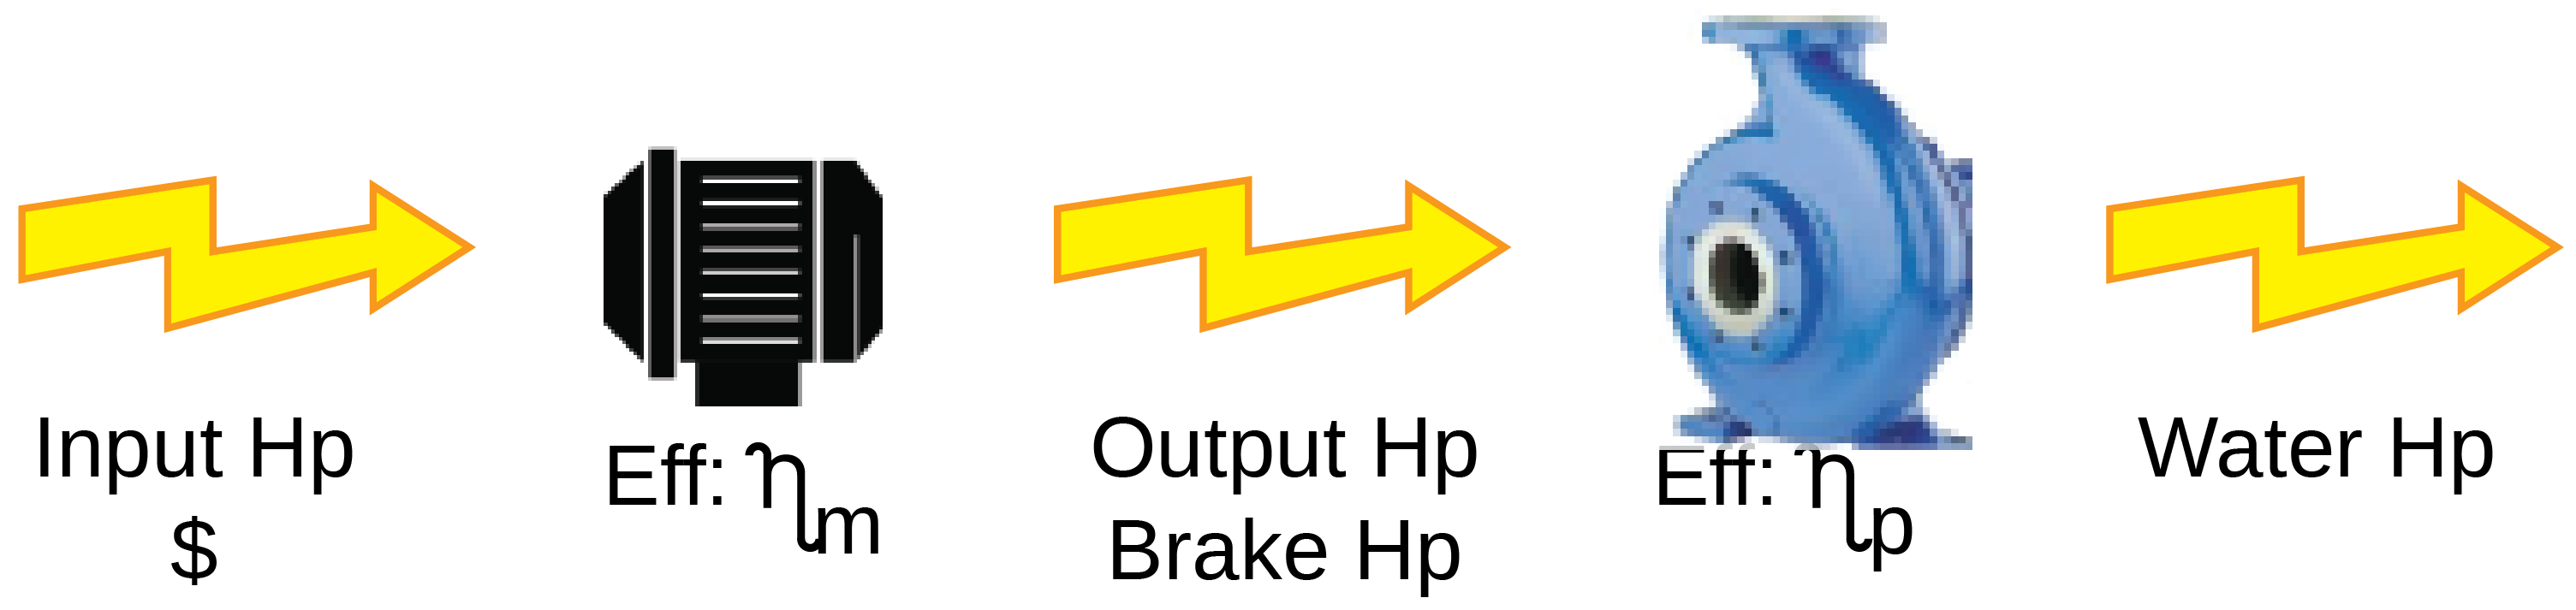
\includegraphics[scale=0.08]{PumpProblem}\\
 \vspace{0.2cm}
 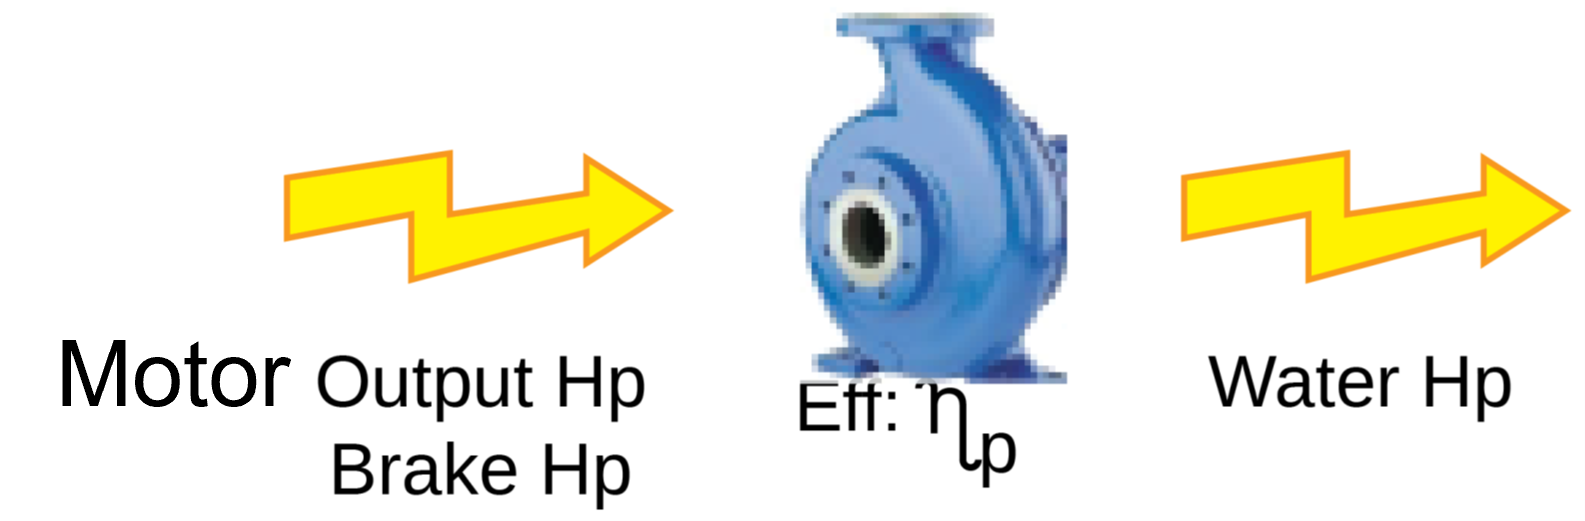
\includegraphics[scale=0.32]{PumpingProblemPump}
 \vspace{0.2cm}

water Hp = flow * head\\
 \vspace{0.2cm}
$\mathrm{Water} \enspace \mathrm{Hp} = 500 \enspace \mathrm{gpm}*50 \enspace ft*\dfrac{\mathrm{Hp}}{3,960 \enspace \mathrm{gpm-ft}}=\boxed{ 6.3 \enspace \mathrm{WHp}}$\\ 
  \vspace{0.2cm}
$\mathrm{Pump \enspace efficiency} =\dfrac{\mathrm{water \enspace Hp}}{\mathrm{brake \enspace Hp}} \implies \mathrm{brake \enspace Hp}=\dfrac{\mathrm{pump \enspace Hp}}{\mathrm{Pump \enspace efficiency}}$ \\
  \vspace{0.2cm}
$\textrm{brake} \enspace Hp = \dfrac{6.3}{0.85}=\boxed{7.4 \enspace \mathrm{Hp}}$\\
  \vspace{0.2cm}
$\mathrm{Motor \enspace efficiency} =\dfrac{\mathrm{brake \enspace Hp}}{\mathrm{input \enspace Hp}} \implies \mathrm{input \enspace \enspace Hp}=\dfrac{\mathrm{brake \enspace Hp}}{\mathrm{motor \enspace efficiency}}= \dfrac{7.4}{0.9}=\boxed{8.2 \enspace \mathrm{Hp}}$\\
  \vspace{0.2cm}
  
 \vspace{0.2cm}
$\mathrm{Wire-to-water} \enspace \mathrm{efficiency}=\eta_m * \eta_p \implies 0.9 \times 0.85 \times 100=\boxed{77 \%}$

\item  Solution:\\
\vspace{0.4cm}
water Hp = flow * head\\
$150 \enspace \mathrm{GPM}*75\mathrm{ft}*\dfrac{Hp}{3,960 GPM-ft}=\boxed{Water \enspace Hp = 2.8Hp}$\\
\vspace{0.4cm}
pump Hp = brake Hp * pump efficiency\\
$brake \enspace Hp = \dfrac{2.8}{0.9}=\boxed{Brake \enspace Hp=3.1Hp}$
 \vspace{0.2cm}

\end{enumerate}






%\chapterimage{FutureChapterImage2.png}
\chapter{Wastewater Treatment - Future}

\section{Water Resource Recovery Facility - WRRF}\index{Water Resource Recovery Facility - WRRF}
\begin{itemize}
\item Originally, the function of a wastewater treatment plant was collection, treatment and disposal which was driven solely by the need to reduce human disease and to protect the environment.
\item It was soon realized that wastewater contains valuable elements like organic matter, phosphorus, nitrogen, rare metals and thermal energy
\item The scope of wastewater treatment has now evolved to encompass recovering valuable resources contained in the wastewater.
\item The wastewater treatment plant is now known as a water resource recovery facility (WRRF). 
\item This change reflects the new focus on the products and benefits of treatment rather than its original and only objective - treating water for sanitation.
\item The WRRF is being adapted into the concept of the circular economy in which products, materials (and raw materials) remain in the economy for as long as possible, and waste is treated as secondary raw materials that can be recycled to process and re-used.  This distinguishes it from a linear economy which is based on the: "take-make-use-dispose" system, in which waste is usually the last stage of the product life cycle.

\end{itemize}

\subsection{Water}\index{Water}
\begin{itemize}
\item Municipal wastewater reuse offers the potential to significantly increase the nation’s total available water resources. Of the 32 billion gallons of treated wastewater discharged nationally, approximately 12 billion gallons of treated wastewater is discharged each day to an ocean or estuary.
\item WRRF is key to the use of treated wastewater, or “reclaimed” water, for beneficial purposes such as drinking, irrigation, or industrial uses—is one option that has helped some communities significantly expand their water supplies.
\item Wastewater can be treated to various qualities to satisfy demand from different sectors, including industry and agriculture. It can be used to maintain the environmental flow, or even reused as drinking water. 
\item Wastewater treatment is one solution to the water scarcity issue, and also to the problem of water security, freeing water resources for other uses or for preservation.
\end{itemize}




\subsection{Energy}\index{Energy}
\begin{itemize}
\item In the US, municipal wastewater treatment plants consume 30 terawatt-hours per year of electricity which is about 0.1\% of the total electrical consumption.  
\item WRRFs have the potential to be energy neutral or even net energy producers through comprehensive energy management approaches, incorporating efficient practices, and generating renewable energy from their by-products, such as biosolids.

\item By making the treatment processes more energy efficient and through the recovery of chemical or calorific energy in the wastewater play a key role in reducing the carbon foot print of the WRRF. 

\item Given the amount of chemical or calorific energy contained in wastewater, the goal is for the WRRFs to be energy neutral or even energy positive - which is to produce same or more energy than the energy needed for treatment.
\end{itemize}


\subsection{Nutrients}\index{Nutrients}
\begin{itemize}
\item Nutrient recovery is the practice of recovering nutrients such as nitrogen and phosphorus from used water streams that would otherwise be discarded/disposed and converting them into fertilizer used for ecological and agricultural purposes. 
\item Phosphate used in fertilizers is manufactured from phosphate rock using a very environmentally detrimental mining process.  Recovery/reuse of phosphate from wastewater mitigates dependence on this mined mineral.
\end{itemize} 
Nutrient recovery at a WRRF is accomplished using one of following two methods:
\begin{enumerate}[1.] 
\item By precipitating phosphorous as struvite crystals using a dedicated reactor. The struvite crystals are collected and resold as fertilizer which has a resale value ranging from \$100-\$600 per dry ton.  Benefits of this method include:
\begin{itemize}
\item Generation of revenue from the fertilizer produced
\item Reduces fouling of equipment due to precipitation of struvite formed during the solids treatment process
\item Allows for meeting NPDES nutrients discharge limits
\end{itemize}
\item Nutrient recovery can also be achieved through the land application of biosolids. Benefits of land application of biosolids include:
\begin{itemize}
\item Provide primary nutrients - nitrogen and phosphorous and secondary nutrients such as calcium, iron, magnesium and zinc for crops.
\item The organic carbon and organic matter in the biosolids help build better soils. 
\item Allows for sequestering carbon in the soil.
\end{itemize}
\end{enumerate}


\section{Challenges to WRRF}\index{Challenges to WRRF}

\subsection{Constituents of Emerging Concern}\index{Constituents of Emerging Concern}
\begin{itemize}
\item Constituents of Emerging Concern (CECs) include a variety of substances such as medicines, personal care products, flame retardants, algal toxins, micorplastics, and many others that are not currently federally regulated but known to occur in water.
\item Some of these CECs, incuding hormones, PFAS, and endocrine disruptors are known to pose health risks to humans and aquatic life.
\item Although some CECs that reach WRRFs are destroyed through wastewater treatment and solids processing, some recalcitrant microconstituents and their metabolites may pass through the treatment process intact and may end up in the effluent or biosolids. 
\item Both, the dose (concentration) of the CEC present and frequency/duration of exposure is important for interpreting possible risk to ecological and human health.
\item The CECs move in their complex cycling through surface and groundwaters across the planet - from potable water to wastewater and viceversa as potable water is converted into wastewater followed by uptake of the treated wastewater by the potable water supply system through groundwater contaminated by the percolation of these CECs in land applied wastewater biosolids or through the CECs in the treated wastewater discharge to surface water such as a lake or river.
\item The CECs concentrations in the plant influent range typically in nano-g/L to micro-g/L , in effluent from non-detect to nano-g/L, and in biosolids the concentrations vary from micro-g/kg to mg/kg.
\end{itemize}


\subsection{Decentralized and Distributed Systems}\index{Decentralized and Distributed Systems}
\begin{itemize}
\item To make the wastewater treatment systems more sustainable and to overcome the issues of a centralized system where wastewater is collected from various areas and cities in urban areas and conveyed to a centrally located plant for treatment, it is imperative to consider 
\item \textbf{Distributed systems} are in different geographical locations, but are linked to a central system either physically, or by management. \textbf{Decentralized systems} can be located in a different geographical location, but are not linked physically, or are not managed under the umbrella of a centralized system.
\item Through the selection of correct locations and appropriate technologies, distributed or decentralized systems can:
\begin{itemize}
\item Provide environmental benefits, such as nutrient and pathogen removal
\item Provide water for direct potable reuse and non-potable water in both rural and urban settings for purposes such as flushing, cooling and heating, landscaping, and subsurface irrigation drip.
\end{itemize}
\end{itemize}


\subsection{Climate Change}\index{Climate Change} 
\begin{itemize}
\item Climate change has directly impacted water resources by altering precipitation patterns, severe drought and floods, snowpack amount, elevation, stream flow, and rising sea levels. 
\item This has created a direct need for utilities to manage local water resources to lessen the potential impact of climate change. 
\item By increasing water reuse, developing resiliency and other actions, WRRFs can be a leader in fighting and preparing for climate change effects.
\item Driven largely by climate change factors, lower carbon footprint - the amount of carbon dioxide and other carbon compounds emitted due to the consumption of fossil fuels (energy), and lower energy demands are now being factored in when assessing wastewater treatment options.
\end{itemize}
\newpage
\begin{center}
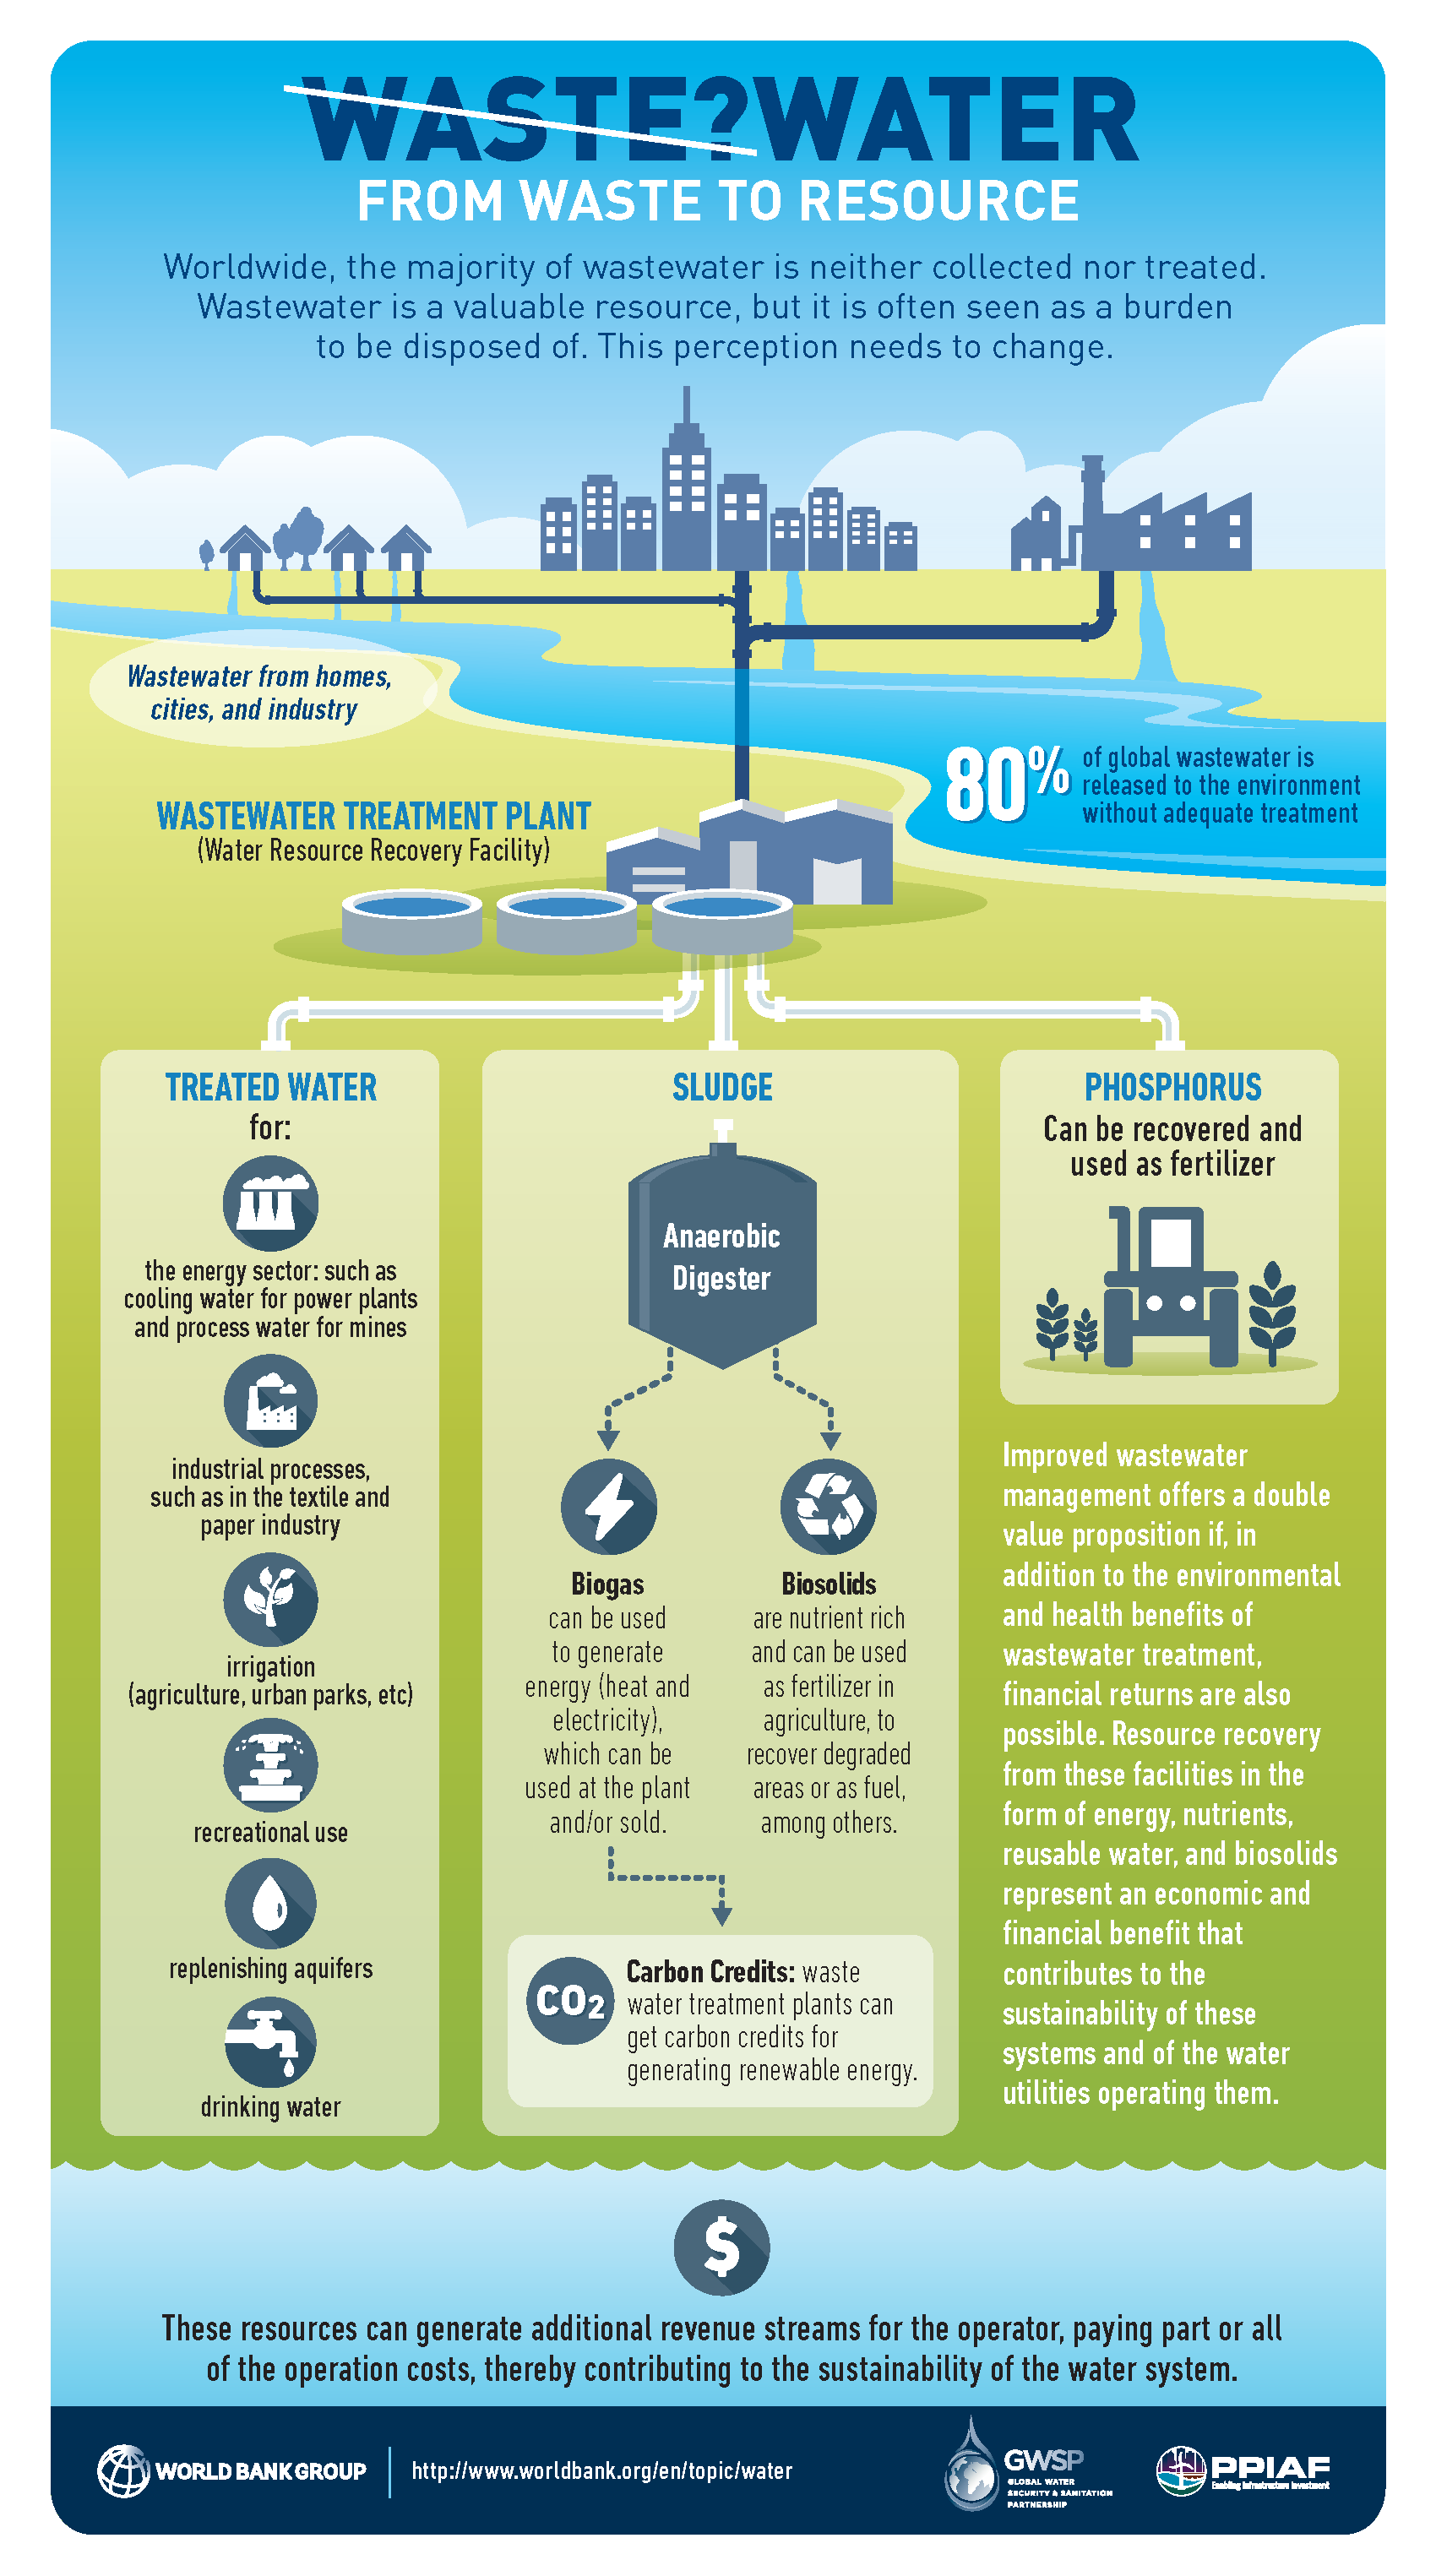
\includegraphics[scale=0.55]{WBWasteWaterResourceinfographic.png}\\
\emph{Source:  Waste to Resource - World Bank}\\
\end{center}









%\chapterimage{CareerChapterImage2.png}
\chapter{Wastewater Treatment - Careers}

\begin{itemize}
\item A career in wastewater treatment provides prospects of a stable and well paid employment with added perk of protecting the environment and the health of the community.
\item Wastewater treatment plants are facing challenges to fill the positions created by the retirement of the baby boomers.  It is estimated 30-50\% of the current employees will retire within the next 10 years.
\item There are a variety of career paths which require different skill sets and training. From high school graduates to PhDs.
\item Although actual renumeration and benefits depend on the size and location of the plant, in general wastewater jobs offer above average wages
\end{itemize}
\vspace{0.3cm}
\begin{tabular}{ |p{5cm}|p{5cm}|p{5cm}|  }
 \hline
 \multicolumn{3}{|c|}{Partial List of Wastewater Career Positions} \\
 \hline
 \hline
Plant Operators   & Collections Workers    &Electrical Maintenance Worker\\
Mechanical Mntnc. Worker   & Construction Inspectors   &Laboratory Technician\\
Environmental Specialists  & Civil Engineers & Mechanical Engineers\\
Electrical Engineers  & Office Assistants & Public Info. Specialists\\
Instrumentation Mntnc. Worker   & Finance and Accounting &Contracts Administrators\\
Warehouse Workers & Buyer & Health and Safety Specialist\\
Surveyors & CAD and Graphics Designers & Planners and Schedulers\\
 \hline
\end{tabular}\\




%%\documentclass{article}
%%\usepackage[english]{babel}%
%\usepackage{graphicx}
%\usepackage{tabulary}
%\usepackage{tabularx}
%\usepackage[table,xcdraw]{xcolor}
%\usepackage{pdflscape}
%\usepackage{lastpage}
%\usepackage{multirow}
%\usepackage{afterpage}
%\usepackage{rotating}
%\usepackage{pdfpages}
%\usepackage{cancel}
%\usepackage{amsmath}
%\usepackage[table]{xcolor}
%\usepackage{caption}
%\captionsetup{font=scriptsize,labelfont=scriptsize}
%\usepackage{pdflscape}
%\usepackage{fixltx2e}
%\usepackage[T1]{fontenc}
%\usepackage[utf8]{inputenc}
%\usepackage{multirow}
%\usepackage{ifthen}
%\usepackage{fancyhdr}
%\usepackage[document]{ragged2e}
%\usepackage[margin=1in,top=1.2in,headheight=57pt,headsep=0.1in]
%{geometry}
%\usepackage{ifthen}
%\usepackage{fancyhdr}
%\everymath{\displaystyle}
%\usepackage[document]{ragged2e}
%\usepackage{fancyhdr}
%\usepackage[table,xcdraw]{xcolor}
%% If you use beamer only pass "xcolor=table" option, i.e. \documentclass[xcolor=table]{beamer}
%\usepackage[normalem]{ulem}
%\useunder{\uline}{\ul}{}
%\everymath{\displaystyle}
%\linespread{2}%controls the spacing between lines. Bigger fractions means crowded lines%
%%\pagestyle{fancy}
%%\usepackage[margin=1 in, top=1in, includefoot]{geometry}
%%\everymath{\displaystyle}
%\linespread{1.3}%controls the spacing between lines. Bigger fractions means crowded lines%
%%\pagestyle{fancy}
%\pagestyle{fancy}
%\setlength{\headheight}{56.2pt}
%
%
%\chead{\ifthenelse{\value{page}=1}{
\includegraphics[scale=0.3]{BassettCTCLogo}\\ \textbf \textbf Water - General Introduction}}
%\rhead{\ifthenelse{\value{page}=1}{Shabbir Basrai}{Shabbir Basrai}}
%\lhead{\ifthenelse{\value{page}=1}{}{\textbf Water - General Introduction}}
%
%
%\cfoot{}
%\lfoot{Page \thepage\ of \pageref{LastPage}}
%\rfoot{}
%\renewcommand{\headrulewidth}{2pt}
%\renewcommand{\footrulewidth}{1pt}
%\newcommand{\comment}[1]{\hspace{0em}{\small\textit{#1}}\bigskip\par}
%\begin{document}


\chapterimage{MathCover.png}
\chapter{Glossary}

ACID :  (1)    A substance that tends to lose a proton. (2)     A substance that dissolves in water with the formation of hydrogen ions. (3)    A substance containing hydrogen which may be replaced with metals to form salts. (4)   A substance that is corrosive.  (5)   A substance that may lower pH\\
\vspace{0.15cm}
ACIDITY :  (A) Measure of the ability to neutralize alkaline (hi pH) substances. (B)  The capacity of water or wastewater to neutralize bases. Acidity is expressed in milligrams per liter of equivalent calcium carbonate.\\
\vspace{0.15cm}
ACRE FOOT :  A volume of water one (1) foot deep and one (1) acre in area, or 43,560 cubic feet.\\
\vspace{0.15cm}
ACTIVATED CARBON :  Form of carbon processed to have small, low–volume pores that increase the surface area available for adsorption or chemical reactions.\\
\vspace{0.15cm}
ACTIVATED SLUDGE :   (A) A biological water treatment technology commonly used in municipal wastewater treatment systems. Sometimes private industry will harness this technique to reduce certain pollutants, such as BOD and COD (see definitions below), but usually only due to compliance concerns.  (B) Sludge withdrawn from the secondary clarifier in the activated sludge process, consisting of micro–organisms, non–living organic matter, and inorganic materials.\\
\vspace{0.15cm}
ACTIVATED SLUDGE PROCESS :   A common method of disposing of pollutants in biological wastewaters. In the process, large quantities of air are bubbled through wastewaters that contain dissolved organic substances in open aeration tanks. Bacteria and other types of microorganisms present in the system need oxygen to live, grown, and multiply in order to consume the dissolved organic "food" or pollutants in the waste. After several hours in a large holding tank, the water is separated from the sludge of bacteria and discharged from the system. Most of the activated sludge is returned to the treatment process, while the remainder is disposed of by one of several acceptable methods.\\
\vspace{0.15cm}
ACTUATOR :   Device used to operate a valve using electric, pneumatic or hydraulic means. Often used for remote control or sequencing of valve operations.\\
\vspace{0.15cm}
ADAPTER SPOOL :   An extension which is added to a short face–to–face valve, to conform to standard API 6D face–to–face dimensions.\\
\vspace{0.15cm}
ADVANCED WASTE TREATMENT :  (A) A treatment technology used to produce an extremely high–quality discharge.  (B) Any process of water renovation that upgrades treated wastewater to meet specific reuse requirements. Typical processes include chemical treatment and pressure filtration.  Also called tertiary treatment.\\
\vspace{0.15cm}
AERATION :   (A) The process of bringing about intimate contact between air and a liquid. (B) The process of adding air to wastewater to provide dissolved oxygen for aerobic bacterial treatment, to freshen wastewater and to keep solids in suspension.\\
\vspace{0.15cm}
AERATION TANK :   A chamber for injecting air into water.\\
\vspace{0.15cm}
AEROBES :  Bacteria that must have molecular (dissolved) oxygen (DO) to survive.\\
\vspace{0.15cm}
AEROBIC :  (A) A condition in which atmospheric or dissolved molecular oxygen is present in the aquatic (water) environment.  (B)  requiring free oxygen for respiration. Refers to types of bacteria commonly found in water and wastewater treatment systems.\\
\vspace{0.15cm}
AEROBIC BACTERIA :  Bacteria which will live and reproduce only in an environment containing oxygen which is available for their respiration (breathing), namely atmospheric oxygen or oxygen dissolved in water. Oxygen combined chemically, such as water molecules (H2O), cannot be used for respiration by aerobic bacteria.\\
\vspace{0.15cm}
AIR END :   A term referring to the side (or parts) of the pump that come into contact with shop/compressed air or natural gas. This applies to any air operated pump including Air Operated Diaphragm Pumps, air operated piston pumps and air operated drum pumps.\\
\vspace{0.15cm}
AIR LIFT :  A type of pump. This device consists of a vertical riser pipe in the wastewater or sludge to be pumped. Compressed air is injected into a tall piece at the bottom of the pipe.   Fine air bubbles mix with the wastewater or sludge to form a mixture lighter than the surrounding water which causes the mixture to rise in the discharge pipe to the outlet. An air–lift pump works like the center of a stand in a percolator coffee pot.\\
\vspace{0.15cm}
AIR TEST :  A method of inspecting a sewer pipe for leaks. Inflatable or similar plugs are placed in the line, and the space between these plugs is pressurized with air. A drop in pressure indicates the line or run being tested has leaks. \\
\vspace{0.15cm}
AIR: operated ejectors or centrifugal pumps. \\
\vspace{0.15cm}
ALGAE :  A class of microscopic plant life that contain chlorophyll, live floating (suspended) in water or are attached to rocks, walls and other surfaces, and grow and multiply through photosynthesis. Algae produce oxygen during sunlight hours, use oxygen during darkness and affect the pH and DO levels in water.\\
\vspace{0.15cm}
ALGAL BLOOM :  Sudden, massive growths of algae that develop in lagoons, lakes and reservoirs.\\
\vspace{0.15cm}
ALIQUOT :  Portion of a sample. Often an equally divided portion of a sample.\\
\vspace{0.15cm}
ALKALINITY :   The capacity of water to neutralize acids, a property imparted by the water’s content of carbonates, bicarbonates, hydroxides, and occasionally borates, silicates, and phosphates. Alkaline fluids have a pH value over 7.\\
\vspace{0.15cm}
ALL WELDED CONSTRUCTION :   Pertains to a valve construction in which the body is completely welded and cannot be disassembled and repaired in the field.\\
\vspace{0.15cm}
ANAEROBIC :   A biological environment that is deficient in all forms of oxygen, especially molecular oxygen, nitrates and nitrites. The decomposition by microorganisms of waste organic matter in wastewater in the absence of dissolved oxygen is classed as anaerobic.\\
\vspace{0.15cm}
ANAEROBIC BACTERIA :  Bacteria that live and reproduce in an environment containing no “free” or dissolved oxygen. Anaerobic bacteria obtain their oxygen supply by breaking down chemical compounds which contain oxygen, such as sulfate (SO 2–).\\
\vspace{0.15cm}
ANAEROBIC DECOMPOSITION :  The decay or breaking down of organic material in an environment containing no “free” or dissolved oxygen. \\
\vspace{0.15cm}
ANAEROBIC DIGESTION :  Anaerobic bacteria (saprophytic and methane fermenters) decompose wastewater solids (complex organic material) in two steps into – 1) volatile acids, and 2) methane gas, carbon dioxide and water in the absence of dissolved oxygen. Specially designed basins, digesters, are used to carry out the digestion processes, prevent air from entering and to capture the methane gas. The sludge layer at the bottom of lagoons provides for similar solids stabilization processes.\\
\vspace{0.15cm}
ANCHOR PIN :   A pin welded onto the body of ball valves. This pin aligns the adapter plate and restrains the plate and gear operator from moving while the valve is being operated.\\
\vspace{0.15cm}
ANGLE VALVE :   A variation of the globe valve, in which the end connections are at right angles to each other, rather than being inline.\\
\vspace{0.15cm}
ANIONIC FLOCCULANT :  Negatively charged flocculant. Used in water treatment to aid solid / liquid separation\\
\vspace{0.15cm}
ANOXIC :   A biological environment that is deficient in molecular oxygen, but may contain chemically bound oxygen, such as nitrates and nitrites.\\
\vspace{0.15cm}
ANOXIC :  Description of an environment without oxygen. In wastewater treatment anoxic processes are typically used for the removal of nitrogen from wastewater.\\
\vspace{0.15cm}
ANTISCALENT :  Material used to control scale formation in water systems such as boiler or cooling water systems.\\
\vspace{0.15cm}
AOD :   AOD stands for Air Operated Diaphragm (pump). These types of pumps are powered by compressed air or gas, making them ideal for hazardous applications such as petroleum based products and other flammable materials. With certain materials of construction, such as steel or conductive plastics, they are easily converted into fully explosion proof (Ex–Proof) pumps. Additionally, they can pull a suction lift and are submersible when installed properly. AOD’s can also handle slurries with solids concentrations up to 30% and can be run against a closed suction or “dead head” situation.\\
\vspace{0.15cm}
AODD :   AODD stands for Air Operated Double Diaphragm (pump). These types of pumps are powered by compressed air or gas, making them ideal for hazardous applications such as petroleum based products and other flammable materials. With certain materials of construction, such as steel or conductive plastics, they are easily converted into fully explosion proof (Ex–Proof) pumps. Additionally, they can pull a suction lift and are submersible when installed properly. AOD’s can also handle slurries with solids concentrations up to 30% and can be run against a closed suction or “dead head” situation.\\
\vspace{0.15cm}
AQUIFER :  A natural underground layer of porous materials usually capable of yielding a supply of water.\\
\vspace{0.15cm}
ARSENIC :   A heavy metal commonly regulated by wastewater discharge permits, but not commonly found in industrial wastewaters. Other heavy metals include – Cadmium (Cd), Chromium(Cr), Copper (Cu), Lead (Pb), Nickel (Ni), and Zinc (Zn).\\
\vspace{0.15cm}
ASPHYXIATION :  An extreme condition often resulting in death due to a lack of oxygen and excess carbon dioxide in the blood from any cause. \\
\vspace{0.15cm}
AVAILABLE CHLORINE :  The amount of chlorine available in compound chlorine sources compared with that of elemental (liquid or gaseous) chlorine.\\
\vspace{0.15cm}
AVERAGE MONTHLY DISCHARGE LIMITATION :  The highest allowable discharge over a calendar month \\
\vspace{0.15cm}
AVERAGE WEEKLY DISCHARGE LIMITATION :  The highest allowable discharge over a calendar week. \\
\vspace{0.15cm}
B.R.V. :  BODY RELIEF VALVE –  A relief valve (optional) installed on ball valves used in liquid service to provide for the relief of excess body pressure caused by thermal expansion.\\
\vspace{0.15cm}
BACK WASH :  Part of water filter, ion exchange or softener cycle that lifts up media bed to release and wash away dirt and other foulants.\\
\vspace{0.15cm}
BACKFILL :  (1) Material used to full in a trench or excavation. (2) The act of filling a trench or excavation, usually after a pipe or some type of structure has been placed in the trench or excavation. \\
\vspace{0.15cm}
BACKFILL COMPACTION :  (1) Tamping, rolling or otherwise mechanically compressing material used as backfill for a trench of excavation. Backfill is compressed to increase its density so that it will support the weight of machinery or other loads after the material is in place  excavation. (2) Compaction of a backfill material can be expressed as a percentage of the maximum compatibility, density or load capacity of the material being used. \\
\vspace{0.15cm}
BACKFLOW :  A reverse flow condition, created by a difference in water pressures, which causes water to flow back into the distribution pipes of a potable water supply from any source or sources other than an intended source. Also see BACKSIPHONAGE.\\
\vspace{0.15cm}
BACKFLUSHING :  A procedure used to wash settled waste matter off upstream to prevent odors from developing after a main line stoppage has been cleared. \\
\vspace{0.15cm}
BACKSEAT :   A Shoulder on the stem of a valve which seals against a mating surface inside the bonnet to permit replacement, under pressure, of stem seals or packing.\\
\vspace{0.15cm}
BACKSIPHONAGE :  A form of backflow caused by a negative or below atmospheric pressure within a water system. Also see BACKFLOW.\\
\vspace{0.15cm}
BACTERIA :   Bacteria are microscopic living organisms They are a group of universally distributed, rigid, essentially unicellular, microscopic organisms lacking chlorophyll. They are characterized as spheroids, rod–like, or curved entities, but occasionally appearing as sheets, chains, or branched filaments.\\
\vspace{0.15cm}
BAFFLE :  A flat board or plate, deflector, guide or similar device constructed or placed in flowing water, wastewater, or slurry systems to cause more uniform flow velocities, to absorb energy, and to divert, guide, or agitate liquids (water, chemical solutions, slurry).\\
\vspace{0.15cm}
BALL :   The spherical closure element of a ball valve.\\
\vspace{0.15cm}
BALL CHECK :   A fitting with a small ball that seals against a seat preventing flow in one direction and allowing flow in the other direction.\\
\vspace{0.15cm}
BALL VALVE :   A valve using a spherical closure element (ball) which is rotated thru 90° to open and close the valve.\\
\vspace{0.15cm}
BALLING :  A method of hydraulically cleaning a sewer or storm drain by using the pressure of a water head to create a high cleansing velocity of water around the ball. In normal operation, the ball is restrained by a cable while water washes past the ball at high velocity. Special sewer cleaning balls have an outside tread that causes them to spin or rotate, resulting in a “scrubbing” action of the flowing water along the pipe wall. \\
\vspace{0.15cm}
BAR RACK :  A screen composed of parallel bars, either vertical or inclined, placed in a sewer or other waterway to catch debris. The screenings may be raked from it. \\
\vspace{0.15cm}
BARREL :  (1) The cylindrical part of a pipe that may have a bell on one end. (2) The cylindrical part of a manhole between the cone at the top and the shelf at the bottom. \\
\vspace{0.15cm}
BASE :  (1)    A substance which takes up or accepts protons.  (2)    A substance which dissociates (separates) in aqueous solution to yield hydroxyl ions (OH–).  (3)    A substance containing hydroxyl ions which reacts with an acid to form a salt or which may react with metalsvto form precipitates.  (4)    A substance that may raise pH.\\
\vspace{0.15cm}
BASE :  A substance that takes up or accepts protons, dissociates in water to produce hydroxyl (OH–) ions, reacts with metals and is corrosive.\\
\vspace{0.15cm}
BDV :  BLOW DOWN VALVE –  A small ball valve that is installed on the aboveground end of an extended drain line. This valve also serves to vent body cavity pressure in the "block and bleed" mode.\\
\vspace{0.15cm}
BEDDING :  The prepared base or bottom of a trench or excavation on which a pipe or other underground structure is supported. \\
\vspace{0.15cm}
BEDDING COMPACTION :  (1) Tamping, rolling or otherwise mechanically compressing material used as bedding for a pipe or other underground structure to a density that will support expected loads. (2) Bedding compaction can be expressed as a percentage of the maximum load capacity of the bedding material. (3) Bedding compaction also can be expressed in load capacity or pounds per square foot. \\
\vspace{0.15cm}
BEDDING GRADE :  (1) In a gravity–flow sewer system, pipe bedding is constructed and compacted to the design grade of the pipe. This is usually expressed in a percentage. A 0.5 percent grade would be a drop of one–half of foot per hundred feet of pipe. (2) Bedding grade for a gravity–flow sewer pipe can also be specified as elevation above mean sea level at specific points. \\
\vspace{0.15cm}
BELL :  (1) In pipe fitting, the enlarged female end of a pipe into which the male end fits. (2) In plumbing, the expanded female end of a wiped joint. \\
\vspace{0.15cm}
BELL: AND–SPIGOT JOINT – A form of joint used on pipes which have an enlarged diameter or bell at one end, and a spigot at the other which fits into and is laid in the bell. The joint is then made tight by lead, cement, rubber O–ring, or other jointing compounds or materials. \\
\vspace{0.15cm}
BELLEVILLE SPRING :   A spring resembling a dished washer, used in some ball valves to push the seats against the ball.\\
\vspace{0.15cm}
BERM :  The earthen dike that surrounds ponds, lagoons and containment areas for hazardous material.\\
\vspace{0.15cm}
BEST EFFICIENCY POINT (B.E.P.) :   The point on a pump’s performance curve that corresponds to the highest efficiency.  \\
\vspace{0.15cm}
BEVEL GEAR OPERATOR :   Device facilitating operation of a gate or globe valve by means of a set of bevel gears having the axis of the pinion gear at right angles to that of the larger ring gear. The reduction ratio of this gearsetdetermines the multiplication of torque achieved.\\
\vspace{0.15cm}
BHP :   BHP is the actual amount of horsepower being consumed by the pump as measured on a pony brake or dynamometer.\\
\vspace{0.15cm}
BIOCHEMICAL OXYGEN DEMAND (BOD) :   A quantitative measure of the oxygen needed by bacteria and micro–organisms for the biological oxidation of organic wastes in a unit volume of wastewater. BOD is generally measured in milligrams per liter (mg/l) of oxygen consumed over a five day period. Although complete biological decomposition of organic waste requires about 20 days, the five day BOD is about two–thirds of the total oxygen required and, therefore, is a practical measure of waste concentration. In waste treatment language, BOD is most frequently stated as the percentage removed during treatment, or remaining after treatment.\\
\vspace{0.15cm}
BIOCIDE :  Chemical substance designed for killing living organisms in water. Often characterized by type of organism killed – bactericide, fungicide or algaecide.\\
\vspace{0.15cm}
BIOLOGICAL OXIDATION :   The process by which bacteria and other types of microorganisms consume dissolved oxygen and organic substances in biological wasterwater.  The energy released is then used to convert organic carbon into carbon dioxide and cellular material. \\
\vspace{0.15cm}
BIOMASS :  Amass or clump of living organisms feeding on wastes in wastewater, dead organisms and other debris. The mass may protect the organisms, as well as store food supplies. Also called ZOOGLEAL MASS.\\
\vspace{0.15cm}
BIOSOLIDS :  A primarily organic solid product, produced by wastewater treatment processes, that can be beneficially recycled. The word biosolids is replacing the word sludge.\\
\vspace{0.15cm}
BIOSOLIDS CAKE :  Solid discharge from a dewatering apparatus. \\
\vspace{0.15cm}
BIT :  (1) Cutting blade used in rodding (pipe cleaning) operations. (2) Cutting teeth on the auger head of a sewer boring tool. \\
\vspace{0.15cm}
BLANK :  A bottle containing only dilution water or distilled water, but the sample being tested is not added. Tests are frequently run on a SAMPLE and a BLANK and the differences are compared.\\
\vspace{0.15cm}
BLOCK AND BLEED :   The capability of obtaining a seal across the upstream and downstream seat rings of a valve when the body pressure is bled off to atmosphere thru blow down valves or vent plugs. Useful in testingfor integrityof seat seals and in accomplishing minor repairs under pressure.\\
\vspace{0.15cm}
BLOCKAGE :  (1) Partial or complete interruption of flow as a result of some obstruction in a sewer. (2) When a collection system becomes plugged and the flow backs up, “blockage.” \\
\vspace{0.15cm}
BLOW DOWN (BLEED: off) – terms to describe the deliberate rejection of water from a system such as boiler or cooling water system. Typically done to control system’s water total dissolved system or conductivity.\\
\vspace{0.15cm}
BLUE: GREEN ALGAE – Varieties of algae characterized by their bluish–green color. The appearance of blue–green algae indicates unhealthy conditions in lagoon cells, often associated with organic overloading and lack of adequate dissolved oxygen.\\
\vspace{0.15cm}
BOD :  Biochemical Oxygen Demand. The rate at which organisms use the oxygen in water or wastewater while stabilizing decomposable organic matter under aerobic conditions. In decomposition, organic matter serves as food for the bacteria and energy results from its oxidation. BOD measurements are used as a measure of the organic strength of wastes in water. \\
\vspace{0.15cm}
BODY :   The principal pressure containing part of a valve, in which the closure element and seats are located.\\
\vspace{0.15cm}
BOLTED BONNET :   A bonnet which is connected to a valve body with bolts or studs and nuts.\\
\vspace{0.15cm}
BOLTED CONSTRUCTION :   Describes a valve construction in which the pressure shell elements are bolted together, and thus can be taken apart and repaired in the field.\\
\vspace{0.15cm}
BONNET :   The top part of a valve, attached to the body, which contains the packing gland, guides the stem, and adapts to extensions or operators.\\
\vspace{0.15cm}
BORE (OR PORT) :   The inside diameter of the smallest opening through a valve, e.g., inside diameter of a seat ring, diameter of hole through ball in a ball valve.\\
\vspace{0.15cm}
BRANCH MANHOLE :  A sewer or drain manhole which has more than one pipe feeding into it. A standard manhole will have one outlet and one inlet. A branch manhole will have one outlet and two or more inlets. \\
\vspace{0.15cm}
BRANCH SEWER :  A sewer that receives wastewater from a relatively small area and discharges into a main sewer servicing more than one branch sewer area. \\
\vspace{0.15cm}
BUBBLE: TIGHT SHUT–OFF –  A phrase used in describing the sealing ability of a valve. During air pressure testing of a new valve in the closed position, leakage past the seats is collected and bubbled thru water. To qualify as "bubble tight," no bubbles should be observed in a prescribed time span.\\
\vspace{0.15cm}
BUCKET :  (1) A special device designed to be pulled along a sewer for the removal of debris from the sewer. The bucket has one end open with the opposite end having a set of jaws. When pulled from the jaw end, the jaws are automatically opened. When pulled from the other end, the jaws close. In operation, the bucket is pulled into the debris from the jaw end and to a point where some of the debris has been forced into the bucket. The bucket is then pulled out of the sewer from the other end, causing the jaws to close and retain the debris. Once removed from the manhole, the bucket is emptied and the process repeated. (2) A conventional pail or bucket used in BUCKETING OUT and also for lowering and raising tools and materials from manholes and excavations. \\
\vspace{0.15cm}
BUCKET BAIL :  The pulling handle on a bucket machine. \\
\vspace{0.15cm}
BUCKET MACHINE : A powered winch machine designed for operation over a manhole. The machine controls the travel of buckets used to clean sewers. \\
\vspace{0.15cm}
BUCKETING OUT :  An expression used to describe removal of debris from a manhole with a pail on a rope. In balling or high–velocity cleaning of sewers, debris is washed into the downstream manhole. Removal of this debris by scooping it into pails and hauling debris out is called “bucketing out.” \\
\vspace{0.15cm}
BUFFER :  A solution or liquid whose chemical makeup neutralizes acids or bases without a great change in pH.\\
\vspace{0.15cm}
BULKING :  Clouds of billowing sludge that occur throughout secondary clarifiers and sludge thickeners when the sludge does not settle properly.   In the activated sludge process bulking is usually caused by filamentous bacteria or bound water.\\
\vspace{0.15cm}
BULKING SLUDGE :   A phenomenon that occurs in activated sludge plants whereby the sludge occupies excessive volumes and will not concentrate readily. This condition refers to a decrease in the ability of the sludge to settle and consequent loss over the settling tank weir. Bulking in activated sludge aeration tanks is caused mainly by excess suspended solids (SS) content. Sludge bulking in the final settling tank of an activated sludge plant may be caused by improper balance of the BOD load, SS concentration in the mixed liquor, or the amount of air used in aeration.\\
\vspace{0.15cm}
BURIED SERVICE :   An application in which valves are installed in lines which are buried below ground level.\\
\vspace{0.15cm}
BUTT WELD END (BWE) :   The end connection of a valve suitably prepared for butt welding to a connecting pipe.\\
\vspace{0.15cm}
BUTTERFLY VALVE :   A short face–to–face valve which has a movable vane, in the center of the flow stream, which rotates 90 degrees as the butterfly valve opens and closes.\\
\vspace{0.15cm}
BVR :  BALL VALVE REGULATOR –  An automatic throttling valve controlling flow or pressure in a pipeline; comprising a package involving al ball valve actuator, positioner, and controlling instrument.\\
\vspace{0.15cm}
BYPASS :   A system of pipes and valves permitting the diversion of flow or pressure around a line valve.\\
\vspace{0.15cm}
BYPASS :  A pipe, valve, gate, weir, trench or other device designed to permit all or part of a wastewater flow to be diverted from usual channels or flow. Sometimes refers to a special line which carries the flow around a facility or device that needs maintenance or repair. \\
\vspace{0.15cm}
BYPASSING :  The act of causing all or part of a flow to be diverted from its usual channels. In a wastewater treatment plant, overload flows should be bypassed into a holding pond for future treatment. 224 \\
\vspace{0.15cm}
CADMIUM :   A heavy metal commonly regulated by wastewater discharge permits and typically found in the metal finishing industry.  Other heavy metals include – Arsenic (As), Chromium(Cr), Copper (Cu), Lead (Pb), Nickel (Ni), and Zinc (Zn).\\
\vspace{0.15cm}
CAKE SOLID DISCHARGE RATE :  The dry solids cake discharge from a centrifuge, which is expressed as: dry cake solids discharge rate = (dry solids feed rate) x (solids recovery). \\
\vspace{0.15cm}
CALCIUM AND MAGNESIUM SOAPS, MINERAL OILS, AND CERTAIN OTHER NON: fatty material which tend to separate from water and coagulate as floatables or scums. \\
\vspace{0.15cm}
CARBON DIOXIDE :  A common gas, CO2, found abundantly in air, is a product of bacterial respiration and used by algae in photosynthesis. The concentration of carbon dioxide in the lagoon water governs the pH of the lagoon.\\
\vspace{0.15cm}
CARCINOGEN :  Any substance that tends to produce cancer in an organism.\\
\vspace{0.15cm}
CASING :   The body of the pump which encloses the impeller. Primarily used in reference to centrifugal pumps.\\
\vspace{0.15cm}
CAST :   The form of a particular part of a valve, where the basic shape is formed by molding rather than fabricating.\\
\vspace{0.15cm}
CASTING :   A product or the act of producing a product made by pouring molten metal into a mold and allowing it to solidify, thus taking the shape of the mold.\\
\vspace{0.15cm}
CATCH BASIN :  A chamber or well used with storm or combined sewers as a means of removing grit which might otherwise enter and be deposited in sewers. \\
\vspace{0.15cm}
CATIONIC FLOCCULANT :  Positively charged high molecular weight polyelectrolyte water soluble organic polymer designed to agglomerate solids in water substrates.\\
\vspace{0.15cm}
CAVITATION :  The formation and collapse of a gas pocket or bubble on the blade of an impeller or gate of a valve. The collapse of the bubble drives water into the impeller or gate with a terrific force that can cause pitting of the surface. Cavitation is indicated by loud hammering noises.\\
\vspace{0.15cm}
CENTRIFUGAL FORCE :   A force associated with a rotating body. In the case of a pump, the rotating impeller pushes fluid on the back of the impeller blade, imparting motion. Since the motion is circular there is a centrifugal force associated with it. The force pushes the fluid against a fixed pump casing thereby pressurizing the fluid and forcing it through the outlet.\\
\vspace{0.15cm}
CENTRIFUGAL PUMP :   Centrifugal pumps are the most common type of pump in use today throughout the world. A centrifugal pump is a rotodynamic pump that uses a rotating impeller to increase the velocity of a fluid. Centrifugal pumps are commonly used to move liquids through a piping system. The fluid enters the pump impeller along or near to the rotating axis and is accelerated by the impeller, flowing radially outward into a diffuser or volute chamber, from there it exits into the downstream piping system. A centrifugal pump works by the conversion of the rotational kinetic energy, typically from an electric motor or engine, to an increased static fluid pressure. This action is described by Bernoulli’s principle. The rotation of the pump impeller imparts kinetic energy to the fluid as it is drawn in from the impeller eye (center) and is forced outward through the impeller vanes to the periphery. As the fluid exits the impeller, the fluid kinetic energy (velocity) is then converted to (static) pressure due to the change in area the fluid experiences in the volute section. Typically, the volute shape of the pump casing (increasing in volume), or the diffuser vanes (which serve to slow the fluid, converting to kinetic energy in to flow) are responsible for the energy conversion. The energy conversion results in an increased pressure on the downstream side of the pump, causing flow.\\
\vspace{0.15cm}
CENTRIFUGE :  A mechanical device that uses centrifugal or rotational forces to separate solids from liquids.\\
\vspace{0.15cm}
CHAIN WHEEL OPERATED VALVE :   An overhead valve operated by a chain drive wheel instead of a handwheel.\\
\vspace{0.15cm}
CHARACTERIZED GATE OR BALL :   A ball or gate, the shape of whose port has been specially altered to provide a specific throttling capability.\\
\vspace{0.15cm}
CHECK VALVE :   A one–directional valve which is opened by the fluid flow in one direction and closed automatically when the flow stops or is reversed.\\
\vspace{0.15cm}
CHEMICAL GROUT :  Two chemical solutions that form a solid when combined. Solidification time is controlled by the strength of the mixtures used and the temperature. \\
\vspace{0.15cm}
CHEMICAL OXYGEN DEMAND (COD) :   A quantitative measure of the amount of oxygen required to oxidize all organic compounds in a unit volume on wastewater – non–biodegradable as well as the BOD. The COD level can be determined more readily than BOD, but this measurement does not indicate how much of the waste can be decomposed by biological oxidation.\\
\vspace{0.15cm}
CHLORINATION :   The application of chlorine to water, sewage, or industrial wastes, generally for the purpose of disinfection, but frequently for accomplishing other chemical or biological wasterwater treatment results.\\
\vspace{0.15cm}
CHLORINATOR :  A metering device which is used to add chlorine to water.\\
\vspace{0.15cm}
CHLORINE CONTACT UNIT :  A baffled basin that provides sufficient time for disinfection to occur.\\
\vspace{0.15cm}
CHLORINE DEMAND :  Chlorine demand is the difference between the amount of chorine added to wastewater and the amount of residual chlorine remaining after a given contact time. Chlorine demand may change with dosage, time temperature, pH, and nature and amount of the impurities in the water.\\
\vspace{0.15cm}
CHLORINE REQUIREMENT :    The amount of chlorine which is needed for a particular purpose. Some reasons for adding chlorine are reducing the number of coliform bacteria (Most Probable Number), obtaining a particular chlorine residual, or oxidizing some substance in the water. In each case a definite dosage of chlorine will be necessary. This dosage is the chlorine requirement.\\
\vspace{0.15cm}
CHLORINE RESIDUAL :  The amount of free chlorine remaining after meeting chlorine demand under given conditions and is necessary to complete disinfection.\\
\vspace{0.15cm}
CHOPPER PUMP :   A chopper pump is a centrifugal pump, which is equipped with a cutting system to facilitate chopping/maceration of solids that are present in the pumped liquid. The main advantage of this type of pump is that it prevents clogging of the pump itself and of the adjacent piping, as all the solids and stringy materials are macerated by the chopping system. Chopper pumps exist in various configurations, including submersible and dry–installed design and they are typically equipped with an electric motor to run the impeller and to provide torque for the chopping system. Due to its high solids handling capabilities, the chopper pump is often used for pumping sewage, sludge, manure slurries, and other liquids that contain large or tough solids.\\
\vspace{0.15cm}
CHROMIUM :   A heavy metal commonly regulated by wastewater discharge permits and found in metals–related industries and products (including stainless steel). It is typically regulated in two forms – total chromium and hexavalent chromium. Other heavy metals include – Arsenic (As), Cadmium (Cd), Copper (Cu), Lead (Pb), Nickel (Ni), and Zinc (Zn).\\
\vspace{0.15cm}
CITY GATE :  CITY GATE STATION –  The metering and pressure reducing station where gas is transferred from a high pressure cross–country transmission line to a low pressure distribution piping system within a city.\\
\vspace{0.15cm}
CLAPPER :   The hinged closure element of a swing check valve.\\
\vspace{0.15cm}
CLARIFICATION :  Any process or processes used to reduce the concentration of suspended matter in a liquid, such as quiescent settling or sedimentation. Lagoons provide clarification across the cells and in quiescent zones in aerated systems, allowing solids to settle into a sludge layer\\
\vspace{0.15cm}
CLARIFIER :   A large, circular or rectangular tank that separates solids from the waste stream by settling or flotation.\\
\vspace{0.15cm}
CLEAN IN PLACE (CIP) :  Method of cleaning the interior surfaces of pipes, vessels, process equipment, filters and associated fittings, without disassembly.\\
\vspace{0.15cm}
CLEAN WATER ACT :  Federal legislation passed in 1972 creating the Environmental Protection Agency, requiring a nationwide system for controlling pollutant discharges and providing for construction and regulation of publicly owned treatment works.\\
\vspace{0.15cm}
CLEANOUT :  An opening (usually covered or capped) in a wastewater collection system used for inserting tools, rods or snakes while cleaning a pipeline or clearing a stoppage. \\
\vspace{0.15cm}
CLOSURE ELEMENT :   The moving part of a valve, positioned in the flowstream which controls flow thru the valve. Ball. Gate, Plug, Clapper, Disc, etc., are specific names for closure elements.\\
\vspace{0.15cm}
CO: precipitation – Term to describe compound used in water treatment to aid precipitation of substances normally soluble under the conditions employed. Common co–precipitants used in water are iron, aluminum, calcium and magnesium.\\
\vspace{0.15cm}
COAGULANTS :  Chemicals that cause very fine particles to clump (floc) together into larger particles. This makes it easier to separate the solids from the water by settling, skimming, draining or filtering.\\
\vspace{0.15cm}
COAGULATION :   The agglomeration of colloidal or suspended matter brought about by the addition of some chemical to the liquid, by contact, or by other means.  Involves destabilization for repulsive electrical charges to permit agglomeration of colloid particles in water. This process aids the clarification of water.\\
\vspace{0.15cm}
COLIFORM :  A type of bacteria. The presence of coliform–group bacteria is an indication of possible pathogenic bacterial contamination. The human intestinal tract is one of the main habitats of coliform bacteria. They may also be found in the intestinal tracts of warm–blooded animals, and in plants, soil, air, and the aquatic environment. Fecal coliforms are those coliforms found in the feces of various warm–blooded animals; whereas the term “coliform” also includes various other environmental sources.\\
\vspace{0.15cm}
COLIFORM :  A type of bacteria. The presence of coliform–group bacteria is an indication of possible pathogenic bacterial contamination. The human intestinal tract is one of the main habitats of coliform bacteria. They may also be found in the intestinal tracts of warm–blooded animals, and in plants, soil, air, and the aquatic environment. Fecal coliforms are those coliforms found in the feces of various warm–blooded animals; whereas the term “coliform” also includes various other environmental sources.\\
\vspace{0.15cm}
COLIFORM BACTERIA :  Live in everyone’s intestinal track. They are considered non–pathogenic. \\
\vspace{0.15cm}
COLIFORM ORGANISMS :   A group of bacteria recognized as indicators of fecal pollution (see also escherichia coliform).\\
\vspace{0.15cm}
COLLECTION SYSTEM :  A network of pipes, manholes, cleanouts, traps, siphons, lift stations and other structures used to collect all wastewater and wastewater–carried wastes of an area and transport them to a treatment plant or disposal system. The collection system includes land, wastewater lines and appurtenances, pumping stations and general property. \\
\vspace{0.15cm}
COLORIMETRIC MEASUREMENT :  A means of measuring unknown chemical concentrations in water by MEASURING A SAMPLE’S COLOR INTENSITY. The specific color of the sample, developed by addition of chemical reagents, is measured with a photoelectric colorimeter or is compared with “color standards” using, or corresponding with, known concentrations of the chemical.\\
\vspace{0.15cm}
COLORIMETRIC MEASUREMENT :  A means of measuring unknown chemical concentrations in water by MEASURING A SAMPLE’S COLOR INTENSITY. The specific color of the sample, developed by addition of chemical reagents, is measured with a photoelectric colorimeter or is compared with “color standards” using, or corresponding with, known concentrations of the chemical.\\
\vspace{0.15cm}
COMBINED SEWER :   Carries both sanitary sewage and storm water run–off.\\
\vspace{0.15cm}
COMMINUTOR :  A device used to reduce the size of the solid chunks in wastewater by shredding (comminuting). The shredding action is like many scissors cutting or chopping to shreds all the large influent solids material in the wastewater.\\
\vspace{0.15cm}
COMMUNITY WASTEWATER SYSTEM :  A public wastewater system which has at least 15 service connection or treats 5,000 gallons or more of wastewater per day. The term “community wastewater system” is used only to identify the public wastewater systems which must be operated by certified operators. \\
\vspace{0.15cm}
COMPOSITE (PROPORTIONAL) SAMPLE :  A collection of individual samples obtained at regular intervals during a 24–hour period. Each individual sample is combined with the others in proportion to the rate of flow when the sample was collected. The resulting mixture, or composite, forms a representative sample and is analyzed to determine the average conditions during the sampling period.\\
\vspace{0.15cm}
COMPUTED PER CAPITA CONTRIBUTION : The computed wastewater contribution from a domestic area, based on the population of the area. In the United States, the daily average wastewater contribution is considered to be 100 gallons per capita per day (100GPCD). \\
\vspace{0.15cm}
COMPUTED TOTAL CONTRIBUTION :  The total anticipated load on a wastewater treatment plant or the total anticipated flow in any collection system area based on the combined computed contributions of all connections to the system. \\
\vspace{0.15cm}
CONCENTRATE :  The high TDS discharge from a reverse osmosis filtration process.\\
\vspace{0.15cm}
CONCRETE CRADLE :  A device made of concrete that is designed to support sewer pipe. 225 \\
\vspace{0.15cm}
CONDENSATE :  steam that has lost heat and condensed into water.\\
\vspace{0.15cm}
CONDUCTIVITY :  Transmittance of an electric current through water. Usually measured in microsiemens per centimeter (uS/cm) or micromho per centimeter (umho/cm).\\
\vspace{0.15cm}
CONFINED SPACE :  Confined space means a space that:  A.     Is large enough and so configured that an employee can bodily enter and perform assigned work; and B.    Has limited or restricted means for entry or exit; and C.     Is not designed for continuous employee occupancy.\\
\vspace{0.15cm}
CONTAMINATION :  The introduction into water of microorganisms, chemicals, toxic substances, wastes, or wastewater in a concentration that makes the water unfit for its next intended use.\\
\vspace{0.15cm}
CONTROL VALVE :   A valve that controls a process variable, such as pressure, flow or temperature by modulating its opening in response to a signal from a controller.\\
\vspace{0.15cm}
CONTROL VOLUME :   Limits imposed for the theoretical study of a system. The limits are usually set to intersect the system at locations where conditions are known.\\
\vspace{0.15cm}
CONTROLLER :   A device that measures a controlled variable, compares it with a predetermined setting and signals the actuator to read just the opening of the valve in order to re–establish the original control setting.\\
\vspace{0.15cm}
COPPER :   A heavy metal commonly regulated by wastewater discharge permits. It is found in the metal finishing and electrical industries. Other heavy metals include – Arsenic (As), Cadmium (Cd), Chromium(Cr), Lead (Pb), Nickel (Ni), and Zinc (Zn).\\
\vspace{0.15cm}
CORROSION :  The gradual decomposition or destruction of a material due to chemical action, often due to an electrochemical reaction. Corrosion starts at the surface of a material and moves inward, such as the chemical action upon manholes and sewer pipe materials. \\
\vspace{0.15cm}
CORROSION INHIBITOR :  chemical additive designed to control / minimize metal corrosion in water system.\\
\vspace{0.15cm}
COULISSE :   Of or using runners or slides as a guiding mechanism; as in a "Coulisse" style gate valve.\\
\vspace{0.15cm}
COUPLING :  (1) A threaded sleeve used to connect two pipes. (2) A device used to connect two adjacent parts, such as pipe coupling, hose coupling or drive coupling. \\
\vspace{0.15cm}
COUPON :  A steel specimen inserted into wastewater to measure the corrosiveness of the wastewater. The rate of corrosion is measured as the loss of weight of the coupon or change in its physical characteristics. Measure the weight loss (in milligrams) per surface area (in square decimeters) exposed to the wastewater per day. \\
\vspace{0.15cm}
CREST :  The bottom edge of a weir plate.\\
\vspace{0.15cm}
CROSS CONNECTION :  A connection between a drinking (potable) water system and an unapproved water supply. For example, if you have a pump moving nonpotable water and hook into the drinking water system to supply water for the pump seal, a cross connection or mixing between the two water systems can occur. This mixing may lead to contamination of the drinking water.\\
\vspace{0.15cm}
CROSS CONNECTION :  A connection between a drinking (potable) water system and an unapproved water supply. For example, if you have a pump moving nonpotable water and hook into the drinking water system to supply water for the pump seal, a cross connection or mixing between the two water systems can occur. This mixing may lead to contamination of the drinking water.\\
\vspace{0.15cm}
CROSS CONNECTION :  A connection between a storm drain system and a sanitary collection system. \\
\vspace{0.15cm}
CROSS: CONNECTION – A connection between a drinking water system and an unapproved system.\\
\vspace{0.15cm}
CRUSTACEANS :  A class of microscopic water animals that consume large quantities of bacteria and algae.\\
\vspace{0.15cm}
CRYOGENIC VALVE :   A valve capable of functioning at cryogenic temperatures.\\
\vspace{0.15cm}
CYANIDE :   A toxic element often found in wastewater from metal finishing industries. It’s commonly regulated by wastewater permits.\\
\vspace{0.15cm}
CYCLE :   A single complete operation or process returning to the starting point. A valve, stroked from full open to full close and back to full open, has undergone one cycle.\\
\vspace{0.15cm}
CYCLES OF CONCENTRATION :  Ratio of boiler or cooling water to make up (feed water). Typically measured by monitoring total dissolved solids, conductivity, silica or chlorides.\\
\vspace{0.15cm}
CYLINDER OPERATOR :   A power–piston valve operator using either hydraulic or pneumatic pressure. A sealed piston converts applied pressure into a linear piston rod (stem) motion.\\
\vspace{0.15cm}
DAILY DISHARGE :  The discharge of a pollutant measured during a calendar day or any 24 – hour period that reasonably represents a calendar day for the purposes of sampling. \\
\vspace{0.15cm}
DAILY MAXIUM DISCHARGE :  The highest allowable value for a daily discharge. \\
\vspace{0.15cm}
DAPHNIA :  A crustacean commonly found in wastewater lagoons.\\
\vspace{0.15cm}
DATUM PLANE :   A reference plane.   A conveniently accessible known surface from which all vertical measurements are taken or referred to.\\
\vspace{0.15cm}
DEADEND MANHOLE :  A manhole located at the upstream end of a sewer and having no inlet pipe. \\
\vspace{0.15cm}
DEBRIS :  Any material in wastewater found floating, suspended, settled, or moving along the bottom of a sewer. This material may cause stoppages by getting hung up on roots or settling out in a sewer. Debris includes grit, paper, rubber, silt, and all materials except liquid. \\
\vspace{0.15cm}
DECHLORINATION :  The removal of chlorine from the effluent of a treatment plant.\\
\vspace{0.15cm}
DECHLORINATION :  The removal of chlorine from the effluent of a treatment plant.\\
\vspace{0.15cm}
DECHLORINATION :  The removal of chlorine from the effluent of a treatment plant.\\
\vspace{0.15cm}
DEMULSIFIER (EMULSION BREAKER) :  Chemical additive that destroys the emulsifying characteristics water. Typically used separate stabilized (emulsified) oil in water.\\
\vspace{0.15cm}
DENITRIFICATION :   A biological process by which nitrate is converted to nitrogen gas.\\
\vspace{0.15cm}
DENITRIFICATION :  (1)     The anoxic biological reduction of nitrate nitrogen to nitrogen gas.  (2)     The removal of some nitrogen from a system.  (3)     An anoxic process that occurs when nitrite or nitrate ions are reduced to nitrogen gas and nitrogen bubbles are formed as a result of this process.\\
\vspace{0.15cm}
DENITRIFICATION :  (1)     The anoxic biological reduction of nitrate nitrogen to nitrogen gas.  (2)     The removal of some nitrogen from a system.  (3)   An anoxic process that occurs when nitrite or nitrate ions are reduced to nitrogen gas and nitrogen bubbles are formed as a result of this process.\\
\vspace{0.15cm}
DENITRIFICATION :  An anaerobic process that occurs when nitrite and nitrate ions are reduced to nitrogen gas and bubbles are formed. These bubbles attach to sludge flocs, causing rising sludge that floats to the surface of secondary clarifiers.\\
\vspace{0.15cm}
DENITRIFICATION :  Wastewater treatment process involved in the biological removal of nitrogen in which the nitrite (NO2) is converted to nitrogen gas (N2)\\
\vspace{0.15cm}
DEQ :  Department of Environmental Quality. \\
\vspace{0.15cm}
DETENTION TIME :  The theoretical time that water may stay in a basin such as lagoon. It is the total volume of the lagoon divided by the flow rate. Usually expressed in days of time or in hours.  The theoretical time water remains in a tank at a given discharge.  The time required to fill a tank at a given flow or the theoretical time required for a given flow of wastewater to pass through a tank.\\
\vspace{0.15cm}
DETRITUS :    The heavy, coarse mixture of grit and organic material carried by wastewater. (also called grit).\\
\vspace{0.15cm}
DEWATER :  To drain or remove water from an enclosure. A structure may be dewatered so that it can be inspected or repaired. Dewater also means draining or removing water from sludge to increase the solids concentration. 226 \\
\vspace{0.15cm}
DEWATERING :  Removing free water from a sludge or slurry to form a high solids cake. belt filter presses, centrifuges, rotary fan presses and vacuum presses are dewatering devices.\\
\vspace{0.15cm}
DEWATERING PUMP :   Any pump capable of removing water from an unwanted area. They are usually small, portable pumps that run on single phase power, compressed air or a small engine, but can be large permanently installed units as well.\\
\vspace{0.15cm}
DIAPHRAGM :   A round, thin flexible sealing device secured and sealed around its outer edge – and sometimes around a central hole in the diaphragm – with its unsupported area free to move by flexing.\\
\vspace{0.15cm}
DICHARGE MONITORING REPORT (DMR) :  The monthly report required by the treatment plant’s NPDES / OPDES discharge permit. \\
\vspace{0.15cm}
DIFFUSED: AIR AERATION – A diffused air activated sludge plant takes air, compresses it, and then discharges the air below the water surface of the aerator through some type of air diffusion device.\\
\vspace{0.15cm}
DIFFUSER :  A device used to break the air stream from the blower system into fine bubbles in an aeration tank or reactor.\\
\vspace{0.15cm}
DIGESTER :  A tank in which sludge is placed to allow decomposition by microorganisms. Digestion may occur under anaerobic (more common) or aerobic conditions.\\
\vspace{0.15cm}
DIGESTION :   The biochemical decomposition of organic matter that results in the formation of mineral and simpler organic compounds.\\
\vspace{0.15cm}
DIP :  A point in the sewer pipe where a drain grade defect results in a puddle of standing water when there is no flow. \\
\vspace{0.15cm}
DIP TUBE :   Extending the blow down valve on large gate valves requires a tube which is located inside of the valve. The tube is called the "dip tube" and extends through the bonnet to the bottom of the body cavity.\\
\vspace{0.15cm}
DISC :   The closure element of a globe angle or small regulator valve. The disc (sometimes referred to as "valve," "poppet" or "plug") moves to and from the seat in a direction perpendicular to the seat face. Depends on stem force for tight shutoff.\\
\vspace{0.15cm}
DISCHARGE STATIC HEAD :   The difference in elevation between the liquid level of the discharge tank and the centerline of the pump. This head also includes any additional head that may be present at the discharge tank fluid surface.\\
\vspace{0.15cm}
DISINFECTION :  The process designed to kill most microorganisms in water, including the destruction or inactivation of pathogenic bacteria. Disinfection differs from sterilization which destroys all living forms.\\
\vspace{0.15cm}
DISINFECTION :  The process designed to kill or inactivate most microorganisms in wastewater, including essentially all pathogenic (disease–casing) bacteria.   There are several ways to disinfect, with chlorination being the most frequently used in water and wastewater treatment plants.\\
\vspace{0.15cm}
DISINFECTION :  The process designed to kill or inactivate most microorganisms in wastewater, including essentially all pathogenic (disease–casing) bacteria.   There are several ways to disinfect, with chlorination being the most frequently used in water and wastewater treatment plants.\\
\vspace{0.15cm}
DISINFECTION :  The process designed to kill or inactivate most microorganisms in water, including essentially all pathogenic (disease–causing) bacteria. There are several ways to disinfect, with chlorine being the most frequently used method in both water and wastewater systems. \\
\vspace{0.15cm}
DISPERSANT :  A non–surface active compound or an active substance added to a suspension, usually a mix, to increase the separation of particles and to prevent subsiding or clumping.\\
\vspace{0.15cm}
DISSOLVED AIR FLOTATION :   A physical/chemical wastewater treatment technology that can be cost–effectively used by industry to remove FOG (fats, oils and grease), suspended solids, and some metals.\\
\vspace{0.15cm}
DISSOLVED AIR FLOTATION CLARIFIER (DAF) :  a piece of equipment that used dissolved air to float suspended solids from water. Typically used when the suspended solids have a lower density than water.\\
\vspace{0.15cm}
DISSOLVED OXYGEN (DO) :   The oxygen dissolved in water, wastewater, or other liquid. DO is measured in milligrams per liter. If the DO of a sample of water is 2 mg/L, it means that there are 2lbs of oxygen in 1 mil lb of water.\\
\vspace{0.15cm}
DISSOLVED SOLIDS :  The salts and other residues left after evaporation of water that has been passed through a laboratory filter. Dissolved solids cannot be filtered out. Some colloidal solids may not be in true solution, but if they pass through the standard membrane filter, they are considered dissolved solids. (See suspended solids)\\
\vspace{0.15cm}
DIURNAL :  Having a daily cycle; usually a 24–hour period from 12:00am to 12:00pm.\\
\vspace{0.15cm}
DO :  Dissolved Oxygen –  An indication of how much oxygen is present in water. If a facility discharges directly to a stream or river, it will usually have a permit limit related to dissolved oxygen.\\
\vspace{0.15cm}
DRAGLINE :  A machine that drags a bucket down the intended line of a trench to dig or excavate the trench. Also used to dig holes and move soil or aggregate. \\
\vspace{0.15cm}
DRAIN PLUG :   A fitting at the bottom of a valve, the removal of which permits draining and flushing the body cavity.\\
\vspace{0.15cm}
DREDGE PUMP :   A dredge pump is a submersible, centrifugal pump capable of handling high solids concentrations and is typically used for clearing out and/or deepening harbors and waterways. The material being moved (i.e.) sand, dirt, soil, etc.) is carried away along with the water it is suspended in.\\
\vspace{0.15cm}
DRIVE PINS :   The two pins which fit into the bottom of a ball valve stem and engage corresponding holes in the ball. As the operator turns the stem, the drive pins turn the ball.\\
\vspace{0.15cm}
DROOP :   A drop in set (outlet) pressure of a regulator or control valve due to the travel of its valve or poppet, as the required flow increases from low to maximum. A slight change in the control spring length due to the valve travel, will result in spring force variations, translating into a change of set (outlet) pressure.\\
\vspace{0.15cm}
DROP MANHOLE :  A main line or house service line lateral entering a manhole at a higher elevation than the main flow line or channel. If the higher elevation flow is routed to the main manhole channel outside of the manhole, it is called an “outside drop.” If the flow is routed down through the manhole barrel, the pipe down to the manhole channel is called an “inside drop.” \\
\vspace{0.15cm}
DRY WELL :  A dry room or compartment in a lift station, near or below the water level, where the pumps are located. \\
\vspace{0.15cm}
DUCKWEED :  A water plant with single small leaf that floats and accumulates on the surface of lagoons.\\
\vspace{0.15cm}
E. COLI OR ESCHERICHIA COLIFORM :   A species of bacteria found in large numbers in the intestinal tract of warm–blooded animals.\\
\vspace{0.15cm}
EASEMENT :  Legal right to use the property of others for a specific purpose. For example, a utility company may have a five–foot easement along the property line of a home. This gives the utility the legal right to install and maintain a sewer line within the easement. \\
\vspace{0.15cm}
EFFICIENCY :   A ratio of total power output to the total power input, expressed as a percent.\\
\vspace{0.15cm}
EFFLUENT :  Wastewater or other liquid—raw (untreated), partially, or completely treated—flowing FROM a reservoir, basin, treatment process, or treatment plant. \\
\vspace{0.15cm}
ELASTOMER :   A natural or synthetic elastic material, often used for o–ring seals. Typical materials are viton, buna–n, EPDM (ethylene propylene dimonomer), etc.\\
\vspace{0.15cm}
ELECTRO DEIONIZATION :  Water treatment technology that utilizes an electricity, ion exchange membranes and resin to deionize water and separate dissolved ions (impurities) from water.\\
\vspace{0.15cm}
ELEVATION :  The height to which something is elevated, such as the height above sea level. \\
\vspace{0.15cm}
ELUTRIATION :  The washing of digested sludge with fresh water, plant effluent or other wastewater. The goal is to remove fine particles and/or the alkalinity in the sludge. This process reduces the demand for conditioning chemicals and improves settling or filtering characteristics of the sludge.\\
\vspace{0.15cm}
ELUTRIATION :  The washing of digested sludge with fresh water, plant effluent or other wastewater. The goal is to remove fine particles and/or the alkalinity in the sludge. This process reduces the demand for conditioning chemicals and improves settling or filtering characteristics of the sludge.\\
\vspace{0.15cm}
EMERGENCY SEAT SEAL :   To obtain tight shut off in an emergency situation, a sealant can be injected into a specially designed groove in the seat rings. Available for most ball valves and gate valves.\\
\vspace{0.15cm}
EMULSION BREAKER (DEMULSIFIER) :  Chemical additive that destroys the emulsifying characteristics water. Typically used separate stabilized (emulsified) oil in water.\\
\vspace{0.15cm}
ENTHALPY :   A thermodynamic property of a fluid. The enthalpy of a fluid consist of the energy associated with the fluid at a microscopic level (related to the temperature of the fluid) plus the energy present in the form of pressure at the inlet and outlet of a system.\\
\vspace{0.15cm}
EODD :   EODD stands for Electrically Operated Double Diaphragm (pumps). These are diaphragm pumps driven either directly or indirectly with an electric motor. Offering many of the same advantages as AOD/AODD pumps with less noise and no compressed air/gas requirements. They cannot run against a closed discharge, which air operated models can, except Graco’s e–Series models.\\
\vspace{0.15cm}
EPA :  United States Environmental Protection Agency. \\
\vspace{0.15cm}
EQUALIZING BASIN :  A holding basin in which variations in flow and composition of a liquid are averaged. Such basins are used to provide a flow of reasonably uniform volume and composition to a treatment unit.  Also called a balancing reservoir.\\
\vspace{0.15cm}
EQUALIZING BASIN :  A holding basin in which variations in flow and composition of a liquid are averaged. Such basins are used to provide a flow of reasonably uniform volume and composition to a treatment unit.  Also called a balancing reservoir.\\
\vspace{0.15cm}
ESCHERICHIA COLIFORM :   A species of bacteria found in large numbers in the intestinal tract of warm–blooded animals.\\
\vspace{0.15cm}
ESDV :  EMERGENCY SHUT DOWN VALVES –  A valve or a system of valves which, when activated, initiate a shut–down of the plant, process, or platform they are tied to.\\
\vspace{0.15cm}
ESTUARY :  Bodies of water that are located at the lower end of a river and are subject to tidal fluctuations.\\
\vspace{0.15cm}
ESTUARY :  Bodies of water that are located at the lower end of a river and are subject to tidal fluctuations.\\
\vspace{0.15cm}
EUTROPHICATION :  The increase of nutrient levels of a lake or other body of water; this usually causes in increase in the growth of aquatic animal and plant life.\\
\vspace{0.15cm}
EUTROPHICATION :  The increase of nutrient levels of a lake or other body of water; this usually causes in increase in the growth of aquatic animal and plant life.\\
\vspace{0.15cm}
EVAPOTRANSPIRATION :  1) The process by which water vapor passes into the atmosphere from living plants. Also called Transpiration.  2) The total water removed from an area by transpiration (living plants) and by evaporation from soil, snow and water surfaces.\\
\vspace{0.15cm}
EVAPOTRANSPIRATION :  1) The process by which water vapor passes into the atmosphere from living plants. Also called Transpiration.  2) The total water removed from an area by transpiration (living plants) and by evaporation from soil, snow and water surfaces.\\
\vspace{0.15cm}
EXFILTRATION :  Liquid wastes and liquid–carried wastes which unintentionally leak out of a sewer pipe system and into the environment. \\
\vspace{0.15cm}
EXPANDING GATE VALVE :   A gate valve that is comprised of a separate gate and segment that as the valve operates the gate and segment move without touching the seats, permitting the valve to be opened and closed without wear. In the closed position the gate and segment are forced against the seat. Continued downward movement of the gate causes the gate and segment to expand against the seats. When the valve reaches its full open position, the gate and segment seal off against the seats while the flow is isolated from the valve body.\\
\vspace{0.15cm}
EXTENDED AERATION :   A modification of the activated sludge process which provides for aerobic sludge digestion within the aeration system.\\
\vspace{0.15cm}
EXTENDED BDV (BLOW DOWN VALVE) :   Used on buried valves where the drain plug is inaccessible. Instead, a line is piped above grade, terminating in a small valve. Line pressure is used to blowout condensates and other material which settles out in the bottom of the body cavity.\\
\vspace{0.15cm}
EXTENSIONS :   The equipment applied to buried valves to provide above grade accessibility to operating gear, blowdown and seat lubrication systems.\\
\vspace{0.15cm}
FACE: TO–FACE –  The overall dimension from the inlet face of a valve to the outlet face of the valve (one end to the other). This dimension is governed by ASME B16.10 and API–6D to ensure that such valves are mutually inter changeable, regardless of the manufacturer.\\
\vspace{0.15cm}
FACULTATIVE :  A combination of both aerobic and anaerobic conditions. Facultative cells have both aerobic and anaerobic zones. Facultative bacteria are able to exist in both aerobic and anaerobic conditions. A facultative pond is commonly used to treat wastewater flows in small communities, It has an upper aerobic zone, a lower anaerobic zone, and algae provide most of the oxygen for the bacteria.\\
\vspace{0.15cm}
FACULTATIVE ORGANISMS :  Organisms that can survive and function in the presence or absence of free, elemental oxygen. Basically, organisms that can switch from aerobic or anaerobic depending on its environment. 227 \\
\vspace{0.15cm}
FACULTATIVE POND (ALSO KNOWN AS A WASTEWATER TREATMENT POND OR LAGOON) :  The most common type of treatment pond used for treating domestic wastewater. The upper portion is aerobic, while the bottom layer is anaerobic. Algae supply most of the oxygen in the aerobic layer. \\
\vspace{0.15cm}
FAIL SAFE VALVE :   A valve designed to fail in a preferred position (open or closed) in order to avoid an undesirable consequence in a piping system.\\
\vspace{0.15cm}
FAIR LEAD PULLEY :  A pulley that is placed in a manhole to guide TV camera electric cables and the pull cable into the sewer when inspecting pipelines. \\
\vspace{0.15cm}
FATS OIL \& GREASE :  a term to describe wastewater contaminants that are commonly found in food or petroleum based effluents. EPA test 1664 is typically used to measure FOG.\\
\vspace{0.15cm}
FATS, OILS, \& GREASE :   Food industry byproducts that can cause significant problems for sewer systems. This pollutant includes both animal/vegetable and petroleum sources and can be regulated separately by these fractions. It is important to know which fraction is regulated and what analytical method is being used to get accurate results.\\
\vspace{0.15cm}
FECAL COLIFORM :  A type of bacteria found in the bodily discharges of warm–blooded animals. Used as an indicator organism. \\
\vspace{0.15cm}
FERMENTATION :  A process of decomposition of organic solid materials by bacteria and other biological actions.\\
\vspace{0.15cm}
FERRIC CHLORIDE :  Metal salt (FeCl3) commonly used as an coagulant in water clarification and as etching agent in chemical–etching.\\
\vspace{0.15cm}
FIELD SERVICEABLE :   A statement indicating that normal repair of the valve or replacement of operating parts can be accomplished in the field without return to the manufacturer.\\
\vspace{0.15cm}
FILAMENTOUS :  The property of growing in long strings, or filaments. Algae and bacteria have filamentous forms. Algae filaments can clog up equipment and be a nuisance in receiving waters. Bacterial filaments area common cause of bulking in activated sludge.\\
\vspace{0.15cm}
FILAMENTOUS ORGANISMS :  Organisms that grow in a thread or filamentous form. Common types are Thiothrix and Actinomycetes. A common cause of sludge bulking in the activated sludge process.\\
\vspace{0.15cm}
FILTER PRESS :  Solids dewatering device that uses pressure differential applied to sludge within a series of plates with filter clothes. The plates (with clothes in them) are arranged in a plate pack with the sludge filling chambers created by recesses within each plate. Filter presses are often called Plate and Frame or Recessed Chamber Filter Presses.\\
\vspace{0.15cm}
FIRE GATE :   A gate or ball valve which is positioned in a pipeline at the entrance to a compressor station. This valve is closed in case of fire in the compressor station. Closing the valve prevents the gas in the pipeline from feeding the fire.\\
\vspace{0.15cm}
FIRE SAFE :   A statement associated with a valve design which is capable of passing certain specified leakage and operational tests after exposure to fire. Must be referenced to a particular specification.\\
\vspace{0.15cm}
FLEXIBLE TUBE VALVE :   A special valve using a flexible sleeve or tube which acts as the closure element. Pressure applied to the jacket space surrounding the outside of the tube, controls the opening and closing of the valve.\\
\vspace{0.15cm}
FLOAT LINE :  A length of rope or heavy twine attached to a float, plastic jug or parachute to be carried by the flow in a sewer from one manhole to the next. This is called “stringing the line” and is used for pulling through winch cables, such as for a bucket machine work or closed–circuit television work. \\
\vspace{0.15cm}
FLOAT VALVE :   A valve which automatically opens or closes as the level of a liquid changes. The valve is operated mechanically by a float which rests on the top of the liquid.\\
\vspace{0.15cm}
FLOATING BALL :   A ball valve having a non–trunnion mounted ball. The ball is free to float between the seat rings, and thus causes higher torques.\\
\vspace{0.15cm}
FLOC :   The agglomeration of smaller particles in a gelatinous mass that can be more easily removed from the liquid than the individual small particles.  Clumps of bacteria and particles or coagulants and impurities that have come together and formed a cluster. Found in aeration tanks, secondary clarifiers and chemical precipitation processes.\\
\vspace{0.15cm}
FLOCCULANT :  high molecular weight polyelectrolyte water soluble organic polymer designed to agglomerate solids in water substrates. Characteristics of flocculants in water treatment are determined by their molecular weight, charge type (anionic, nonionic or cationic) and charge density.\\
\vspace{0.15cm}
FLOCCULATION :  the agglomeration of settleable solids through a bridging mechanism to produce larger particle that is more easily separated from water.\\
\vspace{0.15cm}
FLOODED SUCTION :   In a flooded suction system, the liquid flows to the pump inlet from an elevated source by means of gravity. This is generally recommended for centrifugal pumps.\\
\vspace{0.15cm}
FLOTATION :  (1) The stress or forces on a pipeline or manhole structure below a water table which tend to lift or float the pipeline or manhole structure. (2) The process of raising suspended matter to the surface of the liquid in a tank where it forms a scum layer that can be removed by skimming. The suspended matter is raised by aeration, the evolution of gas, the use of chemicals, electrolysis, heat or bacterial decomposition. \\
\vspace{0.15cm}
FLOW :   A measure of the liquid volume capacity of a pump. Given in gallons per minute/hour (gpm, gph), liters per minute/hour (L/min, L/hour), milliliters per minute (mL/min), cubic meters per hour (m3/h) and other rarely used measurements.\\
\vspace{0.15cm}
FLOW :  The continuous movement of a liquid from one place to another. \\
\vspace{0.15cm}
FLOW ISOLATION :  A procedure used to measure inflow and infiltration (I/I). A section of sewer is blocked off or isolated and the flow from the section is measured. \\
\vspace{0.15cm}
FLUME :  (1) An open conduit of wood, masonry, metal, or plastic constructed on a grade and sometimes elevated. (2) A flow rate measurement device. \\
\vspace{0.15cm}
FLUSHER BRANCH :  A line built specifically to allow the introduction of large quantities of water to the collection system so the lines can be “flushed out” with water. Also installed to provide access for equipment to clear stoppages in a sewer. \\
\vspace{0.15cm}
FLUSHING :  The removal of deposits of material which have lodged in sewers because of inadequate velocity of flows. Water is discharged into the sewers at such rates that the larger flow and higher velocities are sufficient to remove the material. \\
\vspace{0.15cm}
FLUX :  the permeate rate per unit area of membrane surface. Typical units are gals per foot of membrane per day (gfd) or liters of permeate per square meter of membrane per hour (lmh).\\
\vspace{0.15cm}
FOOD: TO–MASS RATIO (F/M) – An activated sludge process–control calculation based upon the amount of food (BOD5 or COD) available per pound of mixed liquor volatile suspended solids. \\
\vspace{0.15cm}
FORCE MAIN :  A pipe that carries wastewater under pressure from the discharge side of a pump to a point of gravity flow downstream.\\
\vspace{0.15cm}
FREE AVAILABLE RESIDUAL CHLORINE :  That portion of the total available chlorine residual composed of dissolved chlorine gas (Cl2), hypochlorous acid (HOCl), and/or hypochlorite ion (OCl–) remaining in water after chlorination.\\
\vspace{0.15cm}
FREE OXYGEN :  Oxygen can be dissolved in water as the soluble gas O2 when it is called free oxygen and measured as dissolved oxygen.\\
\vspace{0.15cm}
FREEBOARD :  The vertical distance from the normal water surface to the top of the confining wall.\\
\vspace{0.15cm}
FRICTION :   The force produced as a reaction to movement. All fluids produce friction when they are in motion. The higher the fluid viscosity, the higher the friction force for the same flow rate. Friction is produced internally as one layer of fluid moves with respect to another and also at the fluid/surface interface.\\
\vspace{0.15cm}
FRICTION HEAD :   The pressure expressed in pounds per square inch or feet of liquid needed to overcome the resistance to the flow in pipes and fittings.\\
\vspace{0.15cm}
FRICTION HEAD DIFFERENCE :   The difference in head required to move a mass of fluid from one position to another at a certain flow rate.\\
\vspace{0.15cm}
FRICTION LOSS :  The head lost by water flowing in a stream or conduit as the result of the disturbances set up by the contact between the moving water and its containing conduit and by intermolecular friction. \\
\vspace{0.15cm}
FULL BORE (FULL PORT) :   Describes a valve in which the bore (port) is nominally equal to the bore of the connecting pipe.\\
\vspace{0.15cm}
FULL OPENING :   Describes a valve whose bore (port) is nominally equal to the bore of the connecting pipe.\\
\vspace{0.15cm}
GAC :  Granular Activated Carbon –  A material used to absorb organics from wastewater. This charcoal–like material can be used in filtration systems to remove solvent contamination.\\
\vspace{0.15cm}
GATE :   The closure element of a gate valve (sometimes called wedge or disc).\\
\vspace{0.15cm}
GATE VALVE :   A straight–thru pattern valve whose closure element is a wedge or parallel–sided slab, situated between two fixed seating surfaces, with means to move it in or out of the flow stream in a direction perpendicular to the pipeline axis.\\
\vspace{0.15cm}
GLAND FOLLOWER OR GLAND FLANGE :   The component used to hold down or retain the gland in the stuffing box.\\
\vspace{0.15cm}
GLAND OR GLAND BUSHING :   That part of a valve which retains or compresses the stem packing in a stuffing box (where used) or retains a stem O–ring, lip seal, or stem O–ring bushing. Sometimes manually adjustable.\\
\vspace{0.15cm}
GLAND PLATE :   The plate in a valve which retains the gland, gland bushing or stem seals and sometimes guides the stem.\\
\vspace{0.15cm}
GLOBE VALVE :   A valve whose closure element is a flat disc or conical plug sealing on a seat which is usually parallel to the flow axis. Can be used for throttling services.\\
\vspace{0.15cm}
GO :  GEAR OPERATED –  The actuation of a valve thru a – ear set which multiplies the torque applied to the valve stem.\\
\vspace{0.15cm}
GRAB SAMPLE :  A single sample of water collected at a particular time and place which represents the composition of water only at that time and place.\\
\vspace{0.15cm}
GRADE :  (1) The elevation of the invert (or bottom) of a pipeline, canal, culvert, sewer, or similar conduit. (2) The inclination of slope of a pipeline, conduit, stream channel, or natural ground surface; usually expressed in terms of the ratio or percentage of number of units of vertical rise or fall per unit of horizontal distance. A 0.5 percent grade would be a drop of one–half foot per hundred feet of pipe. \\
\vspace{0.15cm}
GRAVITY FLOW :  Water or wastewater flowing from a higher elevation to a lower elevation due to the force of gravity. The water does not flow due to energy provided by a pump. Wherever possible, wastewater collection systems are designed to use the force of gravity to convey waste liquids and solids. \\
\vspace{0.15cm}
GREASE :   In wastewater, a group of substances, including fats, waxes, free fatty acids, calcium and magnesium soaps, mineral oils, and certain other non–fatty materials.\\
\vspace{0.15cm}
GREASE :  In a collection system, grease is considered to be the residues of fats, detergents, waxes, free fatty acids, \\
\vspace{0.15cm}
GREASE BUILDUP :  Any point in a collection system where coagulated and solidified greases accumulate and build up. Many varieties of grease have high adhesive characteristics and collect other solids, forming restrictions and stoppages in collection systems. \\
\vspace{0.15cm}
GREASE FITTING :   A fitting through which lubricant or sealant is injected.\\
\vspace{0.15cm}
GREASE TRAP :  A receptacle designed to collect and retain grease and fatty substances usually found in kitchens or from similar wastes. It is installed in the drainage system between the kitchen or other point of production of the waste and the building wastewater collection line. Commonly used to control grease from restaurants. \\
\vspace{0.15cm}
GREEN ALGAE :  The common forms of algae in an aerobic lagoon environment. Green algae are essential for lagoon treatment.\\
\vspace{0.15cm}
GRINDER PUMP :   A grinder pump is a waste management device. Waste from water–using household appliances (toilets, bathtubs, washing machines, etc.) flows through the home’s pipes into the grinder pump’s holding tank. Once the waste inside the tank reaches a certain level, the pump will turn on, grind the waste into fine slurry, and pump it to the central sewer system.\\
\vspace{0.15cm}
GRIT :  The heavy mineral material present in wastewater such as sand, coffee grounds, eggshells, gravel and cinders. Grit tends to settle out at flow velocities below 2 ft. /sec, \\
\vspace{0.15cm}
GRIT CATCHER :  A chamber usually placed at the upper end of a depressed collection line or at other points on combined or storm water collection lines where wear from grit is possible. The chamber is sized and shaped to reduce the velocity of flow through it and thus permit the settling out of grit. \\
\vspace{0.15cm}
GRIT REMOVAL :  Grit removal is accomplished by providing an enlarged channel or chamber which causes the flow velocity to be reduced and allows the heavier grit to settle to the bottom of the channel where it can be removed.\\
\vspace{0.15cm}
GRIT REMOVAL :  Grit removal is accomplished by providing an enlarged channel or chamber which causes the flow velocity to be reduced and allows the heavier grit to settle to the bottom of the channel where it can be removed.\\
\vspace{0.15cm}
GRIT TRAP :  A permanent structure built into a manhole (or other convenient location in a collection system) for the accumulation and easy removal of grit. \\
\vspace{0.15cm}
HAND WHEEL :   A wheel–shaped valve operating device intended to be grasped with one or both hands which allows turning the valve stem or operator shaft to which it is attached.\\
\vspace{0.15cm}
HARD FACING :   A surface preparation in which an alloy is deposited on a metal surface usually by weld overlay to increase resistance to abrasion and or corrosion.\\
\vspace{0.15cm}
HARD WATER :  Water having a high concentration of calcium and magnesium ions.\\
\vspace{0.15cm}
HARDNESS :  It is typically the concentration of calcium and magnesium salts in water. However, it may include other metal salts such as Al, Mn, Sr and Zn. Normally measured as CaCO3 equivalents.\\
\vspace{0.15cm}
HEAD :   Refers to the pressure produced by a vertical column of fluid.  It is a measure of pressure, expressed in feet of head for pumps. Water is used as the default where 10 meters (33.9 ft.) of water equals one atmosphere (14.7 psi. or 1 bar).\\
\vspace{0.15cm}
HEAD :  The vertical distance (in feet) equal to the pressure (in psi) at a specific point. The pressure head is equal to the pressure in psi times 2.31 ft/psi.\\
\vspace{0.15cm}
HEADWORKS :   The part of wastewater treatment where the raw sewage is first received for treatment.  Preliminary treatment occurs at the Headworks.\\
\vspace{0.15cm}
HETEROTROPH :  a type of bacteria that uses organic matter for energy and can use free oxygen, nitrates or sulfates as and oxygen source for respiration.\\
\vspace{0.15cm}
HUBS :   The end connection tubes on a gate valve.\\
\vspace{0.15cm}
HUMAN MACHINE INTERFACE (HMI) :   An interface such as a display screen that permits interaction between a human being and a device/equipment or process. HMI allows for the visual display of status and condition of a particular process or equipment.\\
\vspace{0.15cm}
HWO :  HANDWHEEL OPERATED –  A valve on which the handwheel drives the stem directly to operate the valve.\\
\vspace{0.15cm}
HYDRAULIC LOADING :  The flow of water per acre of surface area.\\
\vspace{0.15cm}
HYDRAULIC MOTOR ACTUATOR (OPERATOR) :   A device by which rotation of a hydraulically powered motor is converted into mechanical motion.\\
\vspace{0.15cm}
HYDROGEN SULFIDE :  A very odorous and poisonous gas. Commonly known as rotten egg gas. It is a combined form of hydrogen and sulfur with the formula H2S.\\
\vspace{0.15cm}
HYDROGEN SULFIDE GAS (H2S) :  Hydrogen sulfide is a gas with a rotten egg odor. This gas is produced under anaerobic conditions.   Hydrogen sulfide is particularly dangerous because it dulls your sense of smell so that you do not notice it after you have been around it for a while and because the odor is not noticeable in high concentrations. The gas is very poisonous to your respiratory system, explosive, flammable and colorless.\\
\vspace{0.15cm}
HYDROLOGIC CYCLE :  The process of evaporation of water into the air and its return to earth by precipitation. (Also called the WATER CYCLE)\\
\vspace{0.15cm}
HYPOCHLORINATORS :  Chlorine pumps, chemical feed pumps or devices used to dispense chlorine solutions made from hypochlorites into the water being treated.\\
\vspace{0.15cm}
IMPELLER :   The rotating element of a centrifugal pump which imparts movement and pressure to a fluid.\\
\vspace{0.15cm}
INCLINED PLATE CLARIFIER :  a solids / liquid separation device (clarifier) that is filled with parallel (sometimes called Lamella) plates that are inclined at an angle between 45 and 55 degrees. The plates reduce (compared to a gravity clarifier) the foot–print required to properly settle solids.\\
\vspace{0.15cm}
INCREMENTAL SEAT TEST :   The leakage testing of valve seats in an assembled valve by increasing the applied pressure in prescribed pressure steps.\\
\vspace{0.15cm}
INDUSTRIAL WASTEWATER :  Wastes associated with industrial manufacturing processes. 229 \\
\vspace{0.15cm}
INFECTION :   Introduction of presence of pathogenic organisms in potable water supply.\\
\vspace{0.15cm}
INFECTION :   Introduction of the presence of pathogenic organisms in potable water supply. This is determined in two ways:\\
\vspace{0.15cm}
INFILTRATION :  The gradual flow of water into the soil; also, the flow of groundwater as seepage into a sewer system.\\
\vspace{0.15cm}
INFILTRATION HEAD :  The distance from a point of infiltration leaking into a collection system to the water table elevation. This is the pressure of the water being forced through the leak in the collection system. \\
\vspace{0.15cm}
INFILTRATION/INFLOW :  The total quantity of water from both infiltration and inflow without distinguishing the source. Abbreviated I\&I or I/I. \\
\vspace{0.15cm}
INFLATABLE PIPE STOPPER :  An inflatable ball or bag used to form a plug to stop flows in a sewer pipe. \\
\vspace{0.15cm}
INFLOW :  Water discharged into a sewer system and service connections from sources other than regular connections. This includes flow from yard drains, foundation drains and around manhole covers. Inflow differs from infiltration in that it is a direct discharge into the sewer rather than a leak in the sewer itself.\\
\vspace{0.15cm}
INFLUENT :  Wastewater or other liquid—raw (untreated) or partially treated—flowing into a reservoir, basin, treatment process, or treatment plant. \\
\vspace{0.15cm}
INLET :  (1) A surface connection to a drain pipe. (2) A chamber for collecting storm water with no well below the outlet pipe for collecting grit. Often connected to a CATCH BASIN or a “basin manhole” with a grit chamber. \\
\vspace{0.15cm}
INLET PORT :   That end of a valve which is connected to the upstream pressure zone of a fluid system.\\
\vspace{0.15cm}
INNER SEAT RING :   The inner part of a two–piece valve seat assembly.\\
\vspace{0.15cm}
INORGANIC :  Material such as salts, metals, and all other substances of mineral origin. \\
\vspace{0.15cm}
INORGANIC :  Material such as sand, salt, iron, calcium salts and other mineral materials and other than of plant or animal origin or of carbon compounds (ORGANIC).\\
\vspace{0.15cm}
INORGANIC MATERIAL :   Material that will not respond to biological action (sand, cinders, stone). Non–volatile fraction of solids.\\
\vspace{0.15cm}
INORGANIC MATERIAL :  Material that will not respond to biological action (sand, cinders, stone). Non–volatile fraction of solids.\\
\vspace{0.15cm}
INSERTION PULLER :  A device used to pull long segments of flexible pipe material into a sewer line when sliplining to rehabilitate a deteriorated sewer. \\
\vspace{0.15cm}
INSIDE: OUT AIR SEAT TEST –  A pressure test that can be performed only on independent seating trunnion mounted ball valves. By closing the valve and pressurizing the body cavity, all of the seals in an independent seating ball valve can then be pressure tested.\\
\vspace{0.15cm}
INSITUFORM :  A method of installing a new pipe within an old pipe without excavation. The process involves the use of a polyester–fiber felt tube, lined on one side with polyurethane and fully impregnated with a liquid thermal setting resin. \\
\vspace{0.15cm}
INSPECTION TELEVISION EQUIPMENT :  Television equipment that is superior to standard commercial quality, providing 600 to 650 lines of resolution, and designed for industrial inspection applications. \\
\vspace{0.15cm}
INTEGRATED FIXED FILM ACTIVATED SLUDGE (IFAS) :   A suspended growth system that provides additional biomass within a biological wastewater treatment system to meet more stringent effluent parameters or increased loadings.\\
\vspace{0.15cm}
INTERNAL PRESSURE RELIEF :   A self relieving feature in non–independent seating valves that automatically relieves excessive internal body pressure caused by sudden changes in line pressures. By means of the piston effect principal the excessive body pressure will move the seat away from its seating surface and relieve it to the lower pressure side.\\
\vspace{0.15cm}
INVERT :  The lowest point of the channel inside a pipe or manhole. \\
\vspace{0.15cm}
INVERTED SIPHON :  A pressure pipeline used to carry wastewater flowing in a gravity collection system under a depression such as a valley or roadway or under a structure such as a building. 230 \\
\vspace{0.15cm}
ION EXCHANGE :  Process that removes dissolved ions from solution of a certain charge by absorption onto a resin that releases (exchanges) an ion of the same charge.\\
\vspace{0.15cm}
ISRS :   Inside screw, rising stem – common term for any valve design in which the stem threads are exposed to the fluid below the packing and the stem rises up through the packing when the valve is opened.\\
\vspace{0.15cm}
KEY MANHOLE :  In collection system evaluation, a key manhole is one from which reliable or specific data can be obtained. \\
\vspace{0.15cm}
KEY STOP :   A method of restricting the travel of a ball valve from fully open to fully closed. The stem key bears against the ends of an arc machined in the adaptor plate.\\
\vspace{0.15cm}
KITE :  A device for hydraulically cleaning sewer lines. Resembling an airport wind sock and constructed of canvas–type material, the kite increases the velocity of a flow at its outlet to wash debris ahead of it. \\
\vspace{0.15cm}
LAMINAR :   A distinct flow regime that occurs at low Reynolds number (Re < 2000). It is characterized by particles in successive layers moving past one another in a well behaved manner (little to no turbulence).\\
\vspace{0.15cm}
LAMPING :  Using reflected sunlight or a powerful light beam to inspect a sewer between two adjacent manholes. The light is directed down the pipe from one manhole. If it can be seen from the next manhole, it indicates that the line is open and straight. \\
\vspace{0.15cm}
LATERAL :  (See LATERAL SEWER) \\
\vspace{0.15cm}
LATERAL CLEANOUT :  A capped opening in a building lateral, usually located on the property line, through which the pipelines can be cleaned. \\
\vspace{0.15cm}
LATERAL SEWER :  A sewer that discharges into a branch or other sewer and has no other common sewer tributary to it. Sometimes called a “street sewer” because it collects wastewater from individual homes. \\
\vspace{0.15cm}
LEAD :   A heavy metal commonly regulated by wastewater discharge permits. Other heavy metals include – Arsenic (As), Cadmium (Cd), Chromium(Cr), Copper (Cu), Nickel (Ni), and Zinc (Zn).\\
\vspace{0.15cm}
LEVER :   A handle type operating device for quarter–turn valves.\\
\vspace{0.15cm}
LIFT STATION :  A wastewater pumping station that lifts the wastewater to a higher elevation when continuing the sewer at reasonable slopes would involve excessive depths of trench. Also, an installation of pumps that raise wastewater from areas too low to drain into available sewers. These stations may be equipped with air–operated ejectors or centrifugal pumps. Sometimes called a PUMP STATION, but this term is usually reserved for a similar type of facility that is discharging into a long FORCE MAIN, while a lift station has a discharge line or force main only up to the downstream gravity sewer. \\
\vspace{0.15cm}
LIFTING LUGS :   Lugs provided on large ball, gate, and check valves, for lifting and positioning valves. Also called lifting eyes.\\
\vspace{0.15cm}
LIMIT SWITCH :   An electrical device providing a signal to a remote observation station indicating when the valve is in the fully open or fully closed position. Usually a component of a valve operator.\\
\vspace{0.15cm}
LIQUID END :   A term referring to the side (or parts) of the pump that come into contact with the process fluid. This applies to any air operated pump including Air Operated Diaphragm Pumps, air operated piston pumps and air operated drum pumps.\\
\vspace{0.15cm}
MAGNETIC DRIVE :   Also referred to as a Mag–drive. This is a method of connecting the motive force to the pump which uses a series of magnets coupled together, with a containment chamber separating them. Magnetic Drives keep the fluid sealed from atmosphere and other environmental factors and eliminate the need for seals and seal maintenance. Special considerations must be taken into account when specifying a Mag–Drive pump or mixer. Ask Springer Pumps for more information.\\
\vspace{0.15cm}
MAIN LINE :  Branch or lateral sewers that collect wastewater from building sewers and service lines. \\
\vspace{0.15cm}
MAIN SEWER :  A sewer line that receives wastewater from many tributary branches and sewer lines and serves as an outlet for a large territory or is used to feed an intercepting sewer. \\
\vspace{0.15cm}
MANDREL :  (1) A special tool used to push bearings in or to pull sleeves out. (2) A gage used to measure for excessive deflection in a flexible conduit. \\
\vspace{0.15cm}
MANHOLE :  An opening in a sewer provided for the purpose of permitting operators or equipment to enter or leave a sewer. \\
\vspace{0.15cm}
MANHOLE ELEVATION :  The height (elevation) of the invert or lowest point in the bottom of a manhole above mean sea level. \\
\vspace{0.15cm}
MANHOLE FLOW :  (1) The depth or amount of wastewater flow in a manhole as observed at any selected time. (2) The total or the average flow through a manhole in gallons on any selected time interval. 231 \\
\vspace{0.15cm}
MANHOLE INFILTRATION :  Groundwater that seeps or leaks into a manhole structure. \\
\vspace{0.15cm}
MANHOLE INFLOW :  Surface waters flowing into a manhole, usually through the vent holes in the manhole lid. \\
\vspace{0.15cm}
MANHOLE INVERT :  The lowest point in a trough or flow channel in the bottom of a manhole. \\
\vspace{0.15cm}
MANHOLE LID :  The heavy cast–iron or forged–steel cover of a manhole. The lid may or may not have vent holes. \\
\vspace{0.15cm}
MANHOLE LID DUST PAN :  A sheet metal or cast–iron pan located under a manhole lid. This pan serves to catch and hold pebbles and other debris falling through vent holes, preventing them from getting into the pipe system. \\
\vspace{0.15cm}
MANHOLE VENTS :  One or a series of one–inch diameter holes through a manhole lid for purposes of venting dangerous gases found in sewers. \\
\vspace{0.15cm}
MASKING AGENTS :  Substances used to cover up or disguise unpleasant odors. Liquid masking agents are dripped into the wastewater, sprayed into the air, or evaporated (using heat) with the unpleasant fumes or odors and then discharged into the air by blowers to make an undesirable odor less noticeable.\\
\vspace{0.15cm}
MASKING AGENTS :  Substances used to cover up or disguise unpleasant odors. Liquid masking agents are dripped into the wastewater, sprayed into the air, or evaporated (using heat) with the unpleasant fumes or odors and then discharged into the air by blowers to make an undesirable odor less noticeable.\\
\vspace{0.15cm}
MBR :  Membrane Bio Reactor –  A wastewater treatment technology that combines biological treatment with physical treatment involving membrane filtration. It’s used primarily to treat BOD, COD, and suspended solids to very low levels where effluent may be able to be reused or recycled.\\
\vspace{0.15cm}
MEAN CELL RESIDENCE TIME (MCRT) :  The average length of time a mixed liquor suspended solids particle remains in the activated sludge process. May also be known as sludge retention time. \\
\vspace{0.15cm}
MECHANICAL AERATION :   Method of aeration.\\
\vspace{0.15cm}
MECHANICAL AERATION :  The use of machinery to mix air and water so that oxygen can be absorbed into the water.\\
\vspace{0.15cm}
MECHANICAL CLEANING :  Clearing pipe by using equipment that scrapes, cuts, pulls or pushes the material out of the pipe. Mechanical cleaning devices or machines include bucket machines, power rodders and hand rods. \\
\vspace{0.15cm}
MECHANICAL PLUG :  A pipe plug used in sewer systems that is mechanically expanded to create a seal. \\
\vspace{0.15cm}
MECHANICAL SEAL :   In a valve, a shut off that is accomplished by a mechanical means rather than with fluid or line pressure. The wedging action of a gate against the seats or the seat springs pushing the seat against the ball or gate are examples of mechanical seals in a valve.\\
\vspace{0.15cm}
MEMBRANE :  Material layer that is a selective barrier between two phases and remains impermeable to specific particles, molecules or substances.\\
\vspace{0.15cm}
MEMBRANE BIO REACTOR :  Aerobic biological wastewater treatment process that utilizes membrane filtration (rather than clarification) for solids / liquid separation. The membrane filters (ultra filters) can be either submerged or external to the biological mixed liquor tanks.\\
\vspace{0.15cm}
MEMBRANE BIOREACTOR (MBR) :   Biological wastewater treatment process where a selected membrane is integrated with a biological process to act as a suspended growth bioreactor.\\
\vspace{0.15cm}
MERCURY (HG) :   A metal which remains liquid at room temperature. This property makes it useful when used in a thin vertical glass tube since small changes in pressure can be measured as changes in the mercury column height. The inch of mercury is often used as a unit for negative pressure.\\
\vspace{0.15cm}
METAL: TO–METAL SEAL –  The seal produced by metal–to–metal contact between the sealing face of the seat ring and the closure element, without benefit of a synthetic seal.\\
\vspace{0.15cm}
METERING PUMP :   Pumps used for precise introductions of chemicals into a tank, existing fluid stream or some other liquid handling equipment. Types of pumps for these include Diaphragm Pumps (AOD or EOD), Peristaltic Pumps, Hose Pumps, Gear Pumps, Bellows Pumps, Piston Pumps and other less commonly used pump types.\\
\vspace{0.15cm}
METHANE :  A combustible gas produced during anaerobic fermentation of organic matter, such as by anaerobic digestion of wastewater solids.\\
\vspace{0.15cm}
MGO :  MANUAL GEAR OPERATOR –  A gear operator that is operated manually (with a handwheel).\\
\vspace{0.15cm}
MGWPCS PERMIT :  Montana Groundwater Pollution Control System permit. This permit is issued to owners/operators of potential sources of pollution to state ground waters.\\
\vspace{0.15cm}
MICRO FILTRATION :  Type of membrane filtration that separates suspended solids and solutes of high molecular from a liquid and low molecular weight solutes. This separation process is used in industry processes, water treatment and research for purifying and concentrating macromolecular solutions.\\
\vspace{0.15cm}
MICRO: Organisms –  Microscopic plans and animals such as bacteria, molds, protozoa, algae, and small metazoa.\\
\vspace{0.15cm}
MICRO: Organisms –  Microscopic plants and animals such as bacteria, molds, protozoa, algae, and small metazoa.\\
\vspace{0.15cm}
MICROORGANISMS :  Microscopic living organisms.\\
\vspace{0.15cm}
MICROORGANISMS :  Very small organisms that can be seen only through a microscope. Some microorganisms use the wastes in wastewater for food and thus remove or alter much of the undesired matter.\\
\vspace{0.15cm}
MILLIGRAMS PER LITER, MG/L :  A measure of the concentration by weight of a substance per unit volume. One thousandth of a gram in one liter. One mg/L is equal to one part per million (ppm).\\
\vspace{0.15cm}
MIXED BED ION EXCHANGE :  Anion exchange process that uses a mixture of cation and anion resin combined in a single ion exchange column. With proper pretreatment, product water purified from a single pass through a mixed bed ion exchange column is the purest that can be made.\\
\vspace{0.15cm}
MIXED LIQUOR :  When the activated sludge in an aeration tank is mixed with primary effluent or the raw wastewater and return sludge, this mixture is then referred to as mixed liquor as long as it is in the aeration tank. Mixed liquor may also refer to the contents of mixed aerobic or anaerobic digesters.\\
\vspace{0.15cm}
MIXED LIQUOR SUSPENDED SOLIDS (MLSS) :   The milligrams of suspended solids per liter of mixed liquor that are combustible at 550 degrees Centigrade. An estimate of the quantity of MLSS to be wasted from the aeration tank of an extended aeration plant may be determined by the rate of settling and centrifuge tests on the sludge solids.\\
\vspace{0.15cm}
MIXED LIQUOR VOLATILE SUSPENDED SOLIDS (MLSS) :  The concentration of organic matter in the mixed liquor suspended solids. \\
\vspace{0.15cm}
MIXED LIQUOR VOLATILE SUSPENDED SOLIDS (MLVSS) :  The organic or volatile suspended solids in the mixed liquor of an aeration tank. This volatile portion is used as a measure or indication of the microorganisms present.\\
\vspace{0.15cm}
MIXED MEDIA GRAVITY FILTER :   A filter using more than one filtering media (such as coal and sand).\\
\vspace{0.15cm}
MIXER, SUBMERSIBLE :   A submersible mixer is a mechanical device that is used to mix sludge tanks and other liquid volumes. Submersible mixers are often used in sewage treatment plants to keep solids in suspension in the various process tanks and/or sludge holding tanks. The submersible mixer is operated by an electric motor, which is coupled to the mixer’s propeller, either direct–coupled or via a planetary gear–reducer. The propeller rotates and creates liquid flow in the tank, which in turn keeps the solids in suspension. The submersible mixer is typically installed on a guide rail system, which enables the mixer to be retrieved for periodic inspection and preventive maintenance.\\
\vspace{0.15cm}
MIXER, VERTICAL :   This style of mixer uses an extended shaft between the motor and mixing blade such that the motor is above and out of the liquid. These also incorporate a gear reducer to slow the speed of the mixing blades to achieve the desired mixing/tank turnover rate. Vertical mixers are often used in reactor vessels to ensure thorough chemical reactions or to mix different ingredients together in food/beverage applications.\\
\vspace{0.15cm}
MOISTURE CONTNET :  The amount of water per unit weight of bio solids. \\
\vspace{0.15cm}
MONITORING WELL :  Wells used to collect groundwater samples for analysis to determine the amount, type, and spread of contaminants in groundwater. Specific design is often determined by the Water Protection Bureau at MT DEQ.\\
\vspace{0.15cm}
MOVING BED BIO REACTOR :   Aerobic biological wastewater treatment process that utilizes the fixed film (media) process. High surface area media is suspended in biological mixed liquor and bacteria grow on the media (attached growth) surface. A clarifier is typically used downstream for solid / liquid separation.\\
\vspace{0.15cm}
MOVING BED BIOREACTOR (MBBR) :   Method to biologically treat wastewater by circulating moving media in an aerobic sludge environment.\\
\vspace{0.15cm}
MPDES PERMIT :  Montana Pollutant Discharge Elimination System permit. This permit lists the conditions that must be met before treatment plants can discharge an effluent into state\\
\vspace{0.15cm}
MULTI: Stage Pump –  The multi–stage pump is used for clean, clear liquids requiring significant discharge pressure. A multi–stage pump is nothing more than a standard centrifugal pump with the discharge of the initial volute discharging directly into the suction of the next volute. The numerous “volutes” are all internal to the pump and many times the volutes are hard to spot individually. The number of stages is dependent on the desired Total Discharge Head required by the application. These types of pump can be either horizontal or vertical configuration. Commonly used for boiler feed.\\
\vspace{0.15cm}
NEEDLE VALVE :   A type of small valve, used for flow metering, having a tapered needle–point plug or closure element and a seat having a small orifice.\\
\vspace{0.15cm}
NEGATIVE PRESSURE :   Pressure that is less than the pressure in the external environment.\\
\vspace{0.15cm}
NEPHELOMETER TURBIDITY UNITS :   It is a measurement of the clarity (turbidity) of a liquid.\\
\vspace{0.15cm}
NEPHELOMETRIC TURBIDITY UNIT :   The standard unit to measure turbidity or how cloudy water is. It’s used as a visual indicator for how well a wastewater treatment system is working.\\
\vspace{0.15cm}
NET POSITIVE SUCTION HEAD (NPSH.) :   The head in feet of water absolute as measured or calculated at the pump suction flange, less the vapor pressure (converted to feet of water absolute) of the fluid.\\
\vspace{0.15cm}
NET POSITIVE SUCTION HEAD AVAILABLE (NPSHA) :   The NPSHa available to prevent cavitation of the pump. To calculate the NPSHa, take the (Static Suction Head) plus (Suction Vessel Surface Pressure Head) minus (vapor pressure of fluid) minus (friction losses in the suction).\\
\vspace{0.15cm}
NET POSITIVE SUCTION HEAD REQUIRED (NPSHR) :   The NPSHr to stop a pump from cavitating. The NPSHr is generally supplied to you by the pump manufacturer.\\
\vspace{0.15cm}
NEWTONIAN FLUID :   A fluid where the relation between shear stress and shear rate is linear, related to viscosity.\\
\vspace{0.15cm}
NICKEL :   A heavy metal commonly regulated by wastewater discharge permits. It can be found in metals–related industries and products, including stainless steel. Other heavy metals include – Arsenic (As), Cadmium (Cd), Chromium(Cr), Copper (Cu), Lead (Pb), and Zinc (Zn).\\
\vspace{0.15cm}
NITRIFICATION :   The conversion of nitrogen matter into nitrates by bacteria.\\
\vspace{0.15cm}
NITRIFICATION :  An aerobic process in which bacteria change ammonia and organic nitrogen into nitrite and nitrate forms of nitrogen.\\
\vspace{0.15cm}
NITRIFICATION :  Wastewater treatment process involved in the biological removal of ammonia in which the ammonia is converted to nitrates (NO3)\\
\vspace{0.15cm}
NITRIFYING BACTERIA :  Bacteria that change the ammonia and organic nitrogen in wastewater into oxidized nitrogen (usually nitrate).\\
\vspace{0.15cm}
NITROGEN :   Nitrogen is present in wastewater in many forms – total Kjeldahl nitrogen, ammonia nitrogen, organic nitrogen.\\
\vspace{0.15cm}
NITROGEN CYCLE :   The cycle of life, death, and decay involving organic nitrogenous matter is known as the nitrogen cycle. In the nitrogen cycle ammonia is produced from proteins.\\
\vspace{0.15cm}
NON: Newtonian Fluid –  A fluid with properties that is different in any way from those of Newtonian Fluids. This is usually found in the relation of viscosity and shear or shear/time.\\
\vspace{0.15cm}
NON: RISING STEM –  A gate valve having its stem threaded into the gate. As the stem turns, the gate moves, but the stem does not rise. Stem threads are exposed to line fluids.\\
\vspace{0.15cm}
NON: Wetted Parts –  A term used any part of a pump, or other type of liquid handling equipment, that doesn’t come into direct contact with the process fluid.\\
\vspace{0.15cm}
NONIONIC :  Neutral charged high molecular weight polyelectrolyte water soluble organic polymer designed to agglomerate solids in water substrates.\\
\vspace{0.15cm}
NONPOINT DISCHARGE :  A source of wastewater that comes from a relatively large area and would have to be controlled by a management or conservation practice. Storm waters and most agricultural waters are nonpoint sources.\\
\vspace{0.15cm}
NONPOTABLE :  Water that is considered unsafe and/or unpalatable for drinking.\\
\vspace{0.15cm}
NONTRANSIENT NONCOMMUNITY (NTNC) WATER SYSTEM :  Means a public water system that is not a community water system and that regularly serves at least 25 of the same persons over six months per year, including schools, day care centers, factories, restaurants and hospitals. 232 \\
\vspace{0.15cm}
NORMALLY CLOSED SOLENOID VALVE :   An electrically operated valve whose inlet orifice is closed when the solenoid coil is not energized. Energize to open.\\
\vspace{0.15cm}
NPDES PERMIT :  National Pollutant Discharge Elimination System permit is the regulatory agency document issued by either a federal or state agency which is designed to control all discharges of pollutants from all point sources and storm water runoff into U.S. waterways. A treatment plant that discharges to a surface water will have a NPDES permit.\\
\vspace{0.15cm}
NRS :  NON–RISING STEM –  A gate valve having its stem threaded into the gate. As the stem turns the gate moves but the stem does not rise. Stem threads are exposed to the line fluid.\\
\vspace{0.15cm}
NUTRIENTS :  Substances required by living plants and organisms. Forms of nitrogen and phosphorous are nutrients that can cause problems in receiving waters.\\
\vspace{0.15cm}
OBSTRUCTION :  Any solid object in or protruding into a wastewater flow in a collection line that prevents a smooth or even passage of the wastewater. \\
\vspace{0.15cm}
OFFSET :  (1) A combination of elbows or bends which brings one section of a line of pipe out of line with, but into a line parallel with, another section. (2) A pipe fitting in the approximate form of a reverse curve, made to accomplish the same purpose. (3) A pipe joint that has lost its bedding support and one of the pipe sections has dropped or slipped, thus creating a condition where the pipes no longer line up properly. \\
\vspace{0.15cm}
OPDES :  Oklahoma Pollutant Discharge Elimination System – A permit program established in accordance with Section 402 of the CWA and authorized in 27A O.S. Environment and Natural Resources. This program regulates discharges into Oklahoma’s waters from point sources, including municipal, industrial, commercial and certain agricultural sources. \\
\vspace{0.15cm}
OPERATING POINT :   The point on the system curve corresponding to the flow and head required to meet the process requirements.\\
\vspace{0.15cm}
OPERATOR :   A device which converts manual, hydraulic, pneumatic or electrical energy into mechanical motion to open and close a valve.\\
\vspace{0.15cm}
ORGANIC :  Material which comes from mainly animal or plant sources and contains carbon. \\
\vspace{0.15cm}
ORGANIC ACIDS :  Weak acids formed from organic compounds, such as acetic acid and citric acid. These acids form first in anaerobic digesters and then are converted to methane. The organic acids in wastewater lagoons are much more complex and generally weaker.\\
\vspace{0.15cm}
ORGANIC MATERIAL :   Carbon based material that can be broken down by bacteria (fats, meats, plant life).  Represents the volatile fraction of solids.\\
\vspace{0.15cm}
ORTHOPHOSPHATE :   A simple compound of phosphorous and oxygen that is soluble in water.\\
\vspace{0.15cm}
OSANDY :  OUTSIDE SCREW AND YOKE –  A valve in which the fluid does not come in contact with the stem threads. The stem sealing elements is between the valve body and the stem threads.\\
\vspace{0.15cm}
OUTFALL :  (1) The point, location or structure where wastewater or drainage discharges from a sewer, drain, or other conduit. (2) The conduit leading to the final disposal point or area. \\
\vspace{0.15cm}
OUTFALL SEWER :  A sewer that receives wastewater from a collection system or from a wastewater treatment plant and carries it to a point of ultimate or final discharge in the environment. \\
\vspace{0.15cm}
OUTLET :  Downstream opening or discharge end of a pipe, culvert, or canal. \\
\vspace{0.15cm}
OVERFLOW MANHOLE :  A manhole which fills and allows raw wastewater to flow out onto the street or ground. \\
\vspace{0.15cm}
OVERFLOW RELIEF LINE :  Where a system has overload conditions during peak flows, an outlet may be installed above the invert and leading to a less loaded manhole or part of the system. This is usually called an “overflow relief line.” \\
\vspace{0.15cm}
OXIC :   A biological environment which is aerobic.\\
\vspace{0.15cm}
OXIDATION :  Oxidation is the addition of oxygen, removal of hydrogen, or the removal of electrons from an element or compound. In wastewater treatment, organic matter is oxidized to more stable substances.\\
\vspace{0.15cm}
OXIDATION :  Oxidation is the addition of oxygen, removal of hydrogen, or the removal of electrons from an element or compound. In wastewater treatment, organic matter is oxidized to more stable substances.\\
\vspace{0.15cm}
OXIDATION POND :  A term often used interchangeably with lagoon. Oxidation ponds are used after other treatment processes.\\
\vspace{0.15cm}
OXIDATION PONDS OR LAGOONS :   Holding ponds designed to allow the decomposition of organic wastes by aerobic or anaerobic means.\\
\vspace{0.15cm}
OXIDATION PONDS OR LAGOONS :   Holding ponds designed to allow the decomposition of organic wastes by aerobic or anaerobic means.\\
\vspace{0.15cm}
OXYGEN REDUCTION POTENTIAL :   A measure that indicates the capacity of wastewater to gain or reduce electrons during a chemical reaction. It is used as a control parameter for treating hexavalent chromium wastewater in the metal finishing industry.\\
\vspace{0.15cm}
PACKAGE TREATMENT PLANT :  A small wastewater treatment plant often fabricated at the manufacturer’s factory, hauled to the site, and installed as one facility. The package may be either a small primary or a secondary wastewater treatment plant.\\
\vspace{0.15cm}
PACKING :   The deformable sealing material inserted into a valve stem stuffing box, which, when compressed by a gland, provides a tight seal about the stem.\\
\vspace{0.15cm}
PALMER: BOWLUS FLUME – A flow measuring device consisting of a preformed flume.\\
\vspace{0.15cm}
PARACHUTE :  A device used to catch wastewater flow to pull a float line between manholes. \\
\vspace{0.15cm}
PARSHALL FLUME :  A flow measuring device consisting of a preformed flume with restrictive area called the throat. The head of water at a stilling well just upstream from the narrow part of the throat is measured and a chart is used to obtain flow rate.\\
\vspace{0.15cm}
PARTS PER BILLION :   A unit of concentration for pollutants in the wastewater. It’s the equivalent of one microgram in 1 liter (ug/l).\\
\vspace{0.15cm}
PARTS PER MILLION :   A unit of concentration for pollutants in the wastewater. It’s the equivalent of 1 milligram in 1 liter (mg/l).\\
\vspace{0.15cm}
PATHOGENIC ORGANISMS :  bacteria, viruses or cysts, which can cause disease (typhoid, cholera, dysentery) in a host such as a human.  Also called Pathogens.\\
\vspace{0.15cm}
PEAKING FACTOR :  Ratio of a maximum flow to the average flow, such as maximum hourly flow or maximum daily flow to the average daily flow. \\
\vspace{0.15cm}
PERCOLATION :  The movement or flow of waster through soil or rocks.\\
\vspace{0.15cm}
PERCOLATION :  The movement or flow of waster through soil or rocks.\\
\vspace{0.15cm}
PERCOLATION :  The movement or flow of water through soil or rocks. A discharge option for many wastewater treatment systems. In Montana, a Montana Ground Water Pollution Control System (MGWPCS) permit and sampling in groundwater monitoring wells are required for permitted systems.\\
\vspace{0.15cm}
PERFORMANCE CURVE :   A curve of flow vs. Total Head for a specific pump model and impeller diameter.\\
\vspace{0.15cm}
PERSONAL COMPUTER (PC) :   Any general–purpose computer whose size, capabilities, and original sales price make it useful for individuals, and which is intended to be operated directly by an end–user with no intervening computer operator.\\
\vspace{0.15cm}
PERSONAL PROTECTIVE EQUIPMENT (PPE) :   Personal protective equipment refers to protective clothing, helmets, goggles or other garments or equipment designed to protect the wearer’s body from injury by blunt impacts, electrical hazards, heat, chemicals and infection, for job–related occupational safety and health purposes.\\
\vspace{0.15cm}
PH :  The intensity of the basic or acid condition of a liquid.\\
\vspace{0.15cm}
PH VALUE :   A convenient method of expressing small differences in the acidity or alkalinity of solutions. Neutrality = pH 7.1; lower values indicate increasing acidity, higher values indicate increasing alkalinity.\\
\vspace{0.15cm}
PH VALUE :   A convenient method of expressing small differences in the acidity or alkalinity of solutions. Neutrality = pH 7.1; lower values indicate increasing acidity, higher values indicate increasing alkalinity.\\
\vspace{0.15cm}
PHOTOGRAPHIC INSPECTIONS :  A method of obtaining photographs of a pipeline by pulling a time–lapse motion picture camera through the line. \\
\vspace{0.15cm}
PHOTOSYNTHESIS :  A complex process in all green plants that contain chlorophyll. The process uses sunlight as energy to convert carbon dioxide into plant growth. As a by–product oxygen is released.\\
\vspace{0.15cm}
PIG :  Refers to a poly pig which is a bullet–shaped device made of hard rubber or similar material. \\
\vspace{0.15cm}
PIPE CAPACITY :  In a gravity–flow sewer system, pipe capacity is the total amount in gallons a pipe is able to pass in a specific time period. \\
\vspace{0.15cm}
PIPE CLEANING :  Removing grease, grit, roots and other debris from a pipe run by means of one of the hydraulic cleaning methods. \\
\vspace{0.15cm}
PIPE DIAMETER :  The nominal or commercially designated inside diameter of a pipe, unless otherwise stated. \\
\vspace{0.15cm}
PIPE DISPLACEMENT :  The cubic inches of soil or water displaced by one foot or one section of pipe. \\
\vspace{0.15cm}
PIPE FRICTION LOSS :   The positive head loss from the friction resistance between the pipe walls and the moving liquid.\\
\vspace{0.15cm}
PIPE GRADE :  The angle of a sewer or a single section of a sewer as installed. Usually expressed in a percentage figure to indicate the drop in feet or tenths of a foot per hundred feet. For example, 0.5 percent grade means a drop of one–half foot per 100 feet of length. \\
\vspace{0.15cm}
PIPE JOINT :  A place where two sections of pipe are coupled or joined together. \\
\vspace{0.15cm}
PIPE JOINT SEAL :  (1) The tightness or lack of leakage at a pipe joint. (2) The method of sealing a pipe coupling. \\
\vspace{0.15cm}
PIPE LINER :  A plastic liner pulled or pushed into a pipe to eliminate excessive infiltration or exfiltration. Other solutions to the problem of infiltration/exfiltration are the use of cement grouting or replacement of damaged pipe. \\
\vspace{0.15cm}
PIPE PLUG :  (1) A temporary plug placed in a sewer pipe to stop a flow while repair work is being accomplished or other functions are performed. (2) In construction of a new sewer system, service saddles are sometimes installed before a building or a building lateral is in existence. Under such circumstances, a plug will be placed in the off–lead of the saddle of a “Y.” \\
\vspace{0.15cm}
PIPE RODDING :  A method of opening a plugged or blocked pipe by pushing a steel rod or snake, or pulling same, through the pipe with a tool attached to the end of the rod or snake. Rotating the rod or snake with a tool attached increases effectiveness. 234 \\
\vspace{0.15cm}
PIPE ROUGHNESS :   A measurement of the average height of peaks producing roughness on the internal surface of pipes. Roughness is measured in many locations, and is usually defined in micro–inches RMS (root mean square).\\
\vspace{0.15cm}
PIPE RUN :  (1) The length of sewer pipe reaching from one manhole to the next. (2) Any length of pipe, generally assumed to be in a straight line. \\
\vspace{0.15cm}
PIPE SECTION :  A single length of pipe between two joints or couplers. \\
\vspace{0.15cm}
PIPING \& INSTRUMENTATION DIAGRAM (P\&ID) :   A diagram in the process industry that shows the piping of the process flow together with the installed equipment and instrumentation.\\
\vspace{0.15cm}
PISTON EFFECT :   The sealing principle involved in utilizing line pressure to effect a seal across the floating seats of some valves.\\
\vspace{0.15cm}
PISTON PUMP :   The piston pump is a positive displacement type of pump. As the piston is pulled back it draws in the fluid, and then as it’s pushed forward it pushes the liquid out. A piston pump can have up to four pistons depending on the application. They should only be used for clear liquids as any solids and/or abrasives in the fluid can damage the pump. Piston pumps are for low flow, high head applications. Frequently used for high–accuracy metering applications.\\
\vspace{0.15cm}
PLAN :  A drawing showing the TOP view of sewers, manholes and streets. Also means approved contract drawings, town standards, working drawings, detail sheets or exact reproductions thereof, which show the location, character, dimensions and details of the work to be done. \\
\vspace{0.15cm}
PLUG :   The rotating closure element of a plug valve. Also a threaded fitting used to close off and seal an opening into a pressure containing chamber, e.g., pipe plug.\\
\vspace{0.15cm}
PLUG VALVE :   A quarter turn valve whose closure element is usually a tapered plug having a rectangular port.\\
\vspace{0.15cm}
PNEUMATIC EJECTOR :  A device for raising wastewater, sludge or other liquid by compressed air. The liquid is alternately admitted through an inward–swinging check valve into the bottom of an airtight pot. When the pot is filled compressed air is applied to the top of the liquid. The compressed air forces the inlet valve closed and forces the liquid in the pot through an outward–swinging check valve, thus emptying the pot. \\
\vspace{0.15cm}
POLISHING POND :  A final lagoon cell after other treatment which completes the treatment, or "polishes" the effluent.\\
\vspace{0.15cm}
POLY PAK STEM SEAL :   An O–ring energized lip–seal which replaces O–ring stem seals in certain gate valves. Also used for stem seals in some ball valves.\\
\vspace{0.15cm}
POLYELECTROLYTES :   Synthetic chemicals used as a coagulant aid.Primary Waste Treatment –  Mechanical separation of solids, grease, and scum from wastewater. With the aid of flocculating agents, primary treatment can eliminate 50 to 65% of the suspended solids. Solids removed by primary treatment may comprise as much as 30 to 40% of the original BOD of the water.\\
\vspace{0.15cm}
POLYMER :  Polymers are used with other chemical coagulants to aid in binding small suspended particles to larger chemical flocs for their removal from water.\\
\vspace{0.15cm}
POLYMER :  Polymers are used with other chemical coagulants to aid in binding small suspended particles to larger chemical flocs for their removal from water.\\
\vspace{0.15cm}
POLYPHOSPHATE :   A large compound formed of several orthophosphate molecules connected by phosphate–storing microorganisms.\\
\vspace{0.15cm}
POLYVINYL CHLORIDE :   The most common material used for wastewater piping. It is a type of plastic.\\
\vspace{0.15cm}
PONDING :  A condition occurring on trickling filters when the hollow spaces (voids) become plugged to the extent that water passage through the filter is inadequate. Ponding may be the result of excessive slime growths, trash, or media breakdown.\\
\vspace{0.15cm}
PONDING :  A condition occurring on trickling filters when the hollow spaces (voids) become plugged to the extent that water passage through the filter is inadequate. Ponding may be the result of excessive slime growths, trash, or media breakdown.\\
\vspace{0.15cm}
POPULATION EQUIVALENT (HYDRAULIC) :  A flow of 100 gallons per day is the hydraulic or flow equivalent to the contribution or flow from one person. Population equivalent = 100 GPCD or gallons per capita per day. \\
\vspace{0.15cm}
POPULATION EQUIVALENT :  An average BOD contribution by each person to a domestic sewage. The accepted population equivalent is 0.17 pounds of BOD per person per day.\\
\vspace{0.15cm}
PORCUPINE :  A sewer cleaning tool the same diameter as the pipe being cleaned. The tool is a steel cylinder having solid ends with eyes cast in them to which a cable can be attached and pulled by a winch. Many short pieces of cable or bristles protrude from the cylinder to form a round brush. \\
\vspace{0.15cm}
POTABLE WATER :   Water fit for human consumption.\\
\vspace{0.15cm}
POTENTIAL ENERGY :   A thermodynamic property. The energy associated with the mass and height of a body above a reference plane.\\
\vspace{0.15cm}
POTENTIAL HYDROGEN :   A measurement of how acidic or basic wastewater is on a scale of 0 to 14.\\
\vspace{0.15cm}
POUNDS PER SQUARE INCH :   A measurement of pressure. It’s often used when discussing physical wastewater treatment technologies involving filtration, but is also used with pumps. Filtration system PSI can indicate when it’s time to backwash or change a filter.\\
\vspace{0.15cm}
POWDER PUMP :   Powder pumps are normally of the Air Operated Diaphragm type and really can pump just powder and powder like materials such as flour and other fine grained, low bulk, dry–density powders in a dust free operation.\\
\vspace{0.15cm}
POWER OPERATOR :   Powered valve operators are of the following general types.. Electric Motor, Pneumatic or Hydraulic Motor, Pheumatic or Hydraulic Cylinder. Operators can either be adapted directly to the valve stem or side mounted on existing gear or scotch–yoke operators.\\
\vspace{0.15cm}
POWER RODDER :  A sewer cleaning machine fitted with auger rods which are inserted in a sewer line to dislodge and cut roots and debris. \\
\vspace{0.15cm}
PPM :  Abbreviation for Parts Per Million. See MILLIGRAMS PER LITER (mg/L)\\
\vspace{0.15cm}
PRE: CLEANING – Sewer line cleaning, commonly done by high–velocity cleaners, that is done prior to the TV inspection of a pipeline to remove grease, slime, and grit to allow for a clearer and more accurate identification of defects and problems. 235 \\
\vspace{0.15cm}
PRECIPITATE :  (1)     An insoluble, finely divided substance which is a product of a chemical reaction within a liquid.  (2)     The separation from solution of an insoluble substance.\\
\vspace{0.15cm}
PRECIPITATION :  (1) The total measurable supply of water received directly from clouds as rain, snow, hail, or sleet; usually expressed as depth in a day, month, or year, and designated as daily, monthly, or annual precipitation. (2) The process by which atmospheric discharged onto a land or water surfaces. (3) The separation (of a substance) out in solid form from a solution, as by the use of a reagent. moisture is \\
\vspace{0.15cm}
PRELIMINARY TREATMENT :  The removal of rocks, rags, sand, eggshells, and similar materials which may hinder the operation of a treatment plant. Preliminary treatment is accomplished by using equipment such as bar screens and grit removal systems. \\
\vspace{0.15cm}
PRESSURE :   The application of external or internal forces to a body producing tension or compression within the body. This tension divided by a surface is called pressure.\\
\vspace{0.15cm}
PRESSURE DROP :   Referring to the loss of pressure between two points in a pipeline system. Generally, this occurs because of pipe friction loss or differences in elevation between the two points.\\
\vspace{0.15cm}
PREVENTIVE MAINTENANCE :  Crews assigned the task of cleaning sewers (for example, balling or high–velocity cleaning crews) to prevent stoppages and odor complaints. Preventive maintenance is performing the most effective cleaning procedure, in the area where it is most needed, at the proper time in order to prevent failures and emergency situations. \\
\vspace{0.15cm}
PRIMARY CELL :  The first cell in a series, generally receiving raw wastewater.\\
\vspace{0.15cm}
PRIMARY CONTAMINANTS :  The contaminants identified by the EPA as harmful to human health. In order to protect public health, the primary contaminants must not exceed certain specified levels known as Maximum Contaminant Levels (MCL). \\
\vspace{0.15cm}
PRIMARY TREATMENT (ALSO KNOWN AS SEDIMENTATION) :  A wastewater treatment process that takes place in a rectangular or circular tank and allows those substances in wastewater that readily settle or float o be separated from the water being treated. \\
\vspace{0.15cm}
PRIMARY WASTE TREATMENT :   Mechanical separation of solids, grease, and scum from wastewater. With the aid of flocculating agents, primary treatment can eliminate 50% t 65% of the suspended solids. Solids removed by the primary treatment may comprise as much as 30% t40% of the original BOD of the water.\\
\vspace{0.15cm}
PROCESS AND INSTRUMENTATION DIAGRAM :   An engineering drawing for a wastewater treatment system. It’s a schematic flow diagram that shows the relationship between different instrumentation and equipment.\\
\vspace{0.15cm}
PROCESS CONTROL :   An engineering discipline that deals with architectures, mechanisms and algorithms for maintaining the output of a specific process within a desired range.\\
\vspace{0.15cm}
PROCESS FLOW DIAGRAM :   A diagram commonly used in engineering to indicate the general flow of plant processes and equipment. The PFD displays the relationship between major equipment of a plant facility and does not show minor details.\\
\vspace{0.15cm}
PROCESS IN WHICH CAVITIES OR BUBBLES FORM IN THE FLUID LOW: pressure area and collapse in a higher pressure area of the pump – causing noise, damage to the pump, and loss of efficiency because it distorts the flow pattern. Occurs in centrifugal pumps when NPSHa < NPSH. A properly designed system and a properly sized pump will prevent cavitation.\\
\vspace{0.15cm}
PROFILE :  A drawing showing the SIDE view of sewers and manholes. \\
\vspace{0.15cm}
PROGRAMMABLE LOGIC CONTROLLER (PLC) :   A microprocessor–based system which provides plant automation by monitoring sensors and controlling actuators and equipment in real time.\\
\vspace{0.15cm}
PROGRESSIVE CAVITY PUMP :   A pump that uses a stator and rotor in a screw shape. The rotor turning inside the stator causes cavities to move in the direction of flow. Progressive Cavity Pumps cannot run dry for any amount of time.\\
\vspace{0.15cm}
PROOF PPRESSURE :   A hydrostatic test pressure, usually 1 ½ times the rated working pressure, applied to an assembled valve to verify the structural integrity of the pressure containing parts. Synonymous with hydrostatic shell test. (Table 5.1, API–6D).\\
\vspace{0.15cm}
PROPELLER PUMP :   Propeller pumps are similar to other centrifugal impeller pumps, but the fluid being pumped is not sent in a circular path. Rather, it proceeds more or less in a straight direction up to the discharge. The motor sits above the discharge shaft. The propeller can be placed below the surface of the liquid, where it will always be primed. Propeller pumps are generally low–speed but low heads. They can be quite large, measuring over a dozen feet in diameter and moving over 50,000 gallons per minute. Some have adjustable–pitch blades.\\
\vspace{0.15cm}
PROTECTIVE SLEEVES :   A circular "pipe like" sleeve inserted in place of the ball and seats of a top entry ball valve. This protective sleeve remains in place inside the valve during valve installation and ultimate pigging of a pipeline to clear debris from the line before placing the pipeline into service. Once the pipeline has been purged of all debris, the protective sleeve is removed entirely from the ball valve cavity and operating trim (i.e. ball and seats) is then installed for normal service conditions.\\
\vspace{0.15cm}
PUBLIC SEWER :  means a sewer in which all owners of abutting properties have equal rights and is controlled by acting as Sewer Commissioners, and maintained by the Public Works Superintendent. \\
\vspace{0.15cm}
PUBLICLY OWNED TREATMENT WORK :   A term to describe a city or municipal sewage treatment facility. Since most industries discharge wastewater to these facilities, they’re typically regulated by these POTWs.\\
\vspace{0.15cm}
PUMP :  A mechanical device for causing flow, for raising or lifting water or other fluid, or for applying pressure to fluids. \\
\vspace{0.15cm}
PUMP CONTROL VALVE :   A ball valve that is not meant for on–off service, but whose specific function is to control flow and prevent cavitation in pumps on liquid pipelines.\\
\vspace{0.15cm}
PUMP IMPELLER :   The moving element in a centrifugal pump that drives the fluid.\\
\vspace{0.15cm}
PUMP PIT :  A dry well, chamber or room below ground level in which a pump is located. \\
\vspace{0.15cm}
PUMP STATION :  Installation of pumps to lift wastewater to a higher elevation in places where flat land would require excessively deep sewer trenches. Also used to raise wastewater from areas too low to drain into available collection lines. These stations may be equipped with \\
\vspace{0.15cm}
RACHET DRIVE :   A shaft or valve that is operated by means of a ratchet mechanism. The ratchet delivers an intermittent stepped rotation through a gear in one direction only.\\
\vspace{0.15cm}
RAW WASTEWATER :   Wastewater before it receives any treatment.\\
\vspace{0.15cm}
REACTOR :   A tank where a wastewater stream is mixed with bacterial sludge and biochemical reactions occur.\\
\vspace{0.15cm}
RECEIVING WATER :  A stream, river, lake, ocean or other surface or groundwater into which treated or untreated wastewater is discharged.\\
\vspace{0.15cm}
RECIRCULATION :  The return of part of the effluent from a treatment process to the incoming flow.\\
\vspace{0.15cm}
REDUCED PORT :   A valve port opening that is smaller than the line size or the valve end connection size.\\
\vspace{0.15cm}
REGULAR PORT VALVE :   A term usually applied to plug valves. The "regular" port of such a valve is customarily about 40% of the line pipe area. Hence, it corresponds to a venture or reduced bor valveof like nominalpipe size. Venturi ball valves are often a logical alternative to plug valves with advantages in price, torque, and low maintenance.\\
\vspace{0.15cm}
REGULATOR :   A throttling valve which exercises automatic control over some variable (usually pressure). Not an on–off valve.\\
\vspace{0.15cm}
RELIEF VALVE :   A quick acting, spring loaded valve that opens (relieves) when the pressure exceeds the spring setting. Often installed on the body cavity of ball and gate valves to relieve thermal overpressure in liquid services.\\
\vspace{0.15cm}
REMOTE CONTROL :   The operation of a valve or other flow control device from a point at a distance from the device being controlled. Can be accomplished by electrical, pneumatic or hydraulic means.\\
\vspace{0.15cm}
RESILIENT SEAT :   A valve seat containing a soft seal, such as an o–ring, to assure tight shut–off.\\
\vspace{0.15cm}
RETENTION :  (1) That part of the precipitation falling on a drainage area which does not escape as surface stream flow during a given period. It is the difference between total precipitation and total runoff during the period, and represents evaporation, transpiration, subsurface leakage, infiltration, and when short periods are considered, temporary surface or underground storage on the area. (2) The delay or holding of the flow of water and water carried wastes in a pipe system. This can be due to a restriction in the pipe, a stoppage or a dip. Also, the time water is held or stored in a basin or wet well. \\
\vspace{0.15cm}
RETENTION TIME :  The time water, sludge or solids are retained or held in a clarifier or sedimentation tank.\\
\vspace{0.15cm}
RETURN ACTIVATED SLUDGE :   Activated return sludge is normally returned continuously to the aeration tank. Recycling of activated sludge back to the aeration tank provides bacteria for incoming wastewater. Its should be brown in color with no obnoxious odor and is often also returned in small portions to the primary settling tanks to aid sedimentation. Settled activated sludge is generally thinner than raw sludge. Some activated sludge will be wasted to prevent excessive solids build up.\\
\vspace{0.15cm}
RETURN ACTIVATED SLUDGE SOLIDS (RASS) :  The concentration of suspended solids in the sludge flow being returned from the settling tank to head of the aeration tank. \\
\vspace{0.15cm}
RETURN SLUDGE :   Settled activated sludge returned to mix with incoming raw or primary settled wastewater. When the return sludge rate in the activated sludge process is too low, there will be insufficient organisms to meet the waste load entering the aerator.\\
\vspace{0.15cm}
REVERSE OSMOSIS :  Water purification technology that uses a semipermeable membrane to remove dissolved solids, molecules and larger particles from water. Applied pressure is used to overcome osmotic pressure and produce high purity water. Reverse osmosis is used to produce ultra pure water for a variety of applications.\\
\vspace{0.15cm}
RIM PULL :   The force required at the edge of the handwheel to generate the required torque at the center of the handwheel.\\
\vspace{0.15cm}
RIP: RAP – Erosion control by placement of large rocks along an embankment.\\
\vspace{0.15cm}
RISING SLUDGE :  Rising sludge occurs in the secondary clarifiers of activated sludge plants when the sludge settles to the bottom of the clarifier, is compacted, and then starts to rise to the surface, usually as a result of denitrification.\\
\vspace{0.15cm}
RISING STEM :   A valve stem which rises as the valve is opened.  A valve stem with threads arranged so that as the stem turns, the threads engage a stationary threaded area and lift the stem along with the closure element attached to it.\\
\vspace{0.15cm}
RISING STEM BALL VALVE :   A single seated ball valve that is designed to seal by using the valves stem to mechanically wedge the valves ball into a stationary seat effecting a bubble tight seal. The valves stem operates througha guide sleeve assembly that guides the stem through a quarter turn of rotation as the stem is raised or lowered by a handwheel (or actuator). The mechanical action of the stem moves the ball away fromthe seat prior to the 90° rotation of the ball. This design provides lower operating torques and longer seat life while assuring bubble tight shut off.\\
\vspace{0.15cm}
ROD (SEWER) :  A light metal rod, three to five feet long with a coupling at each end. Rods are joined and pushed into a sewer to dislodge obstructions. \\
\vspace{0.15cm}
ROD GUIDE :  A bent pipe inserted in a manhole to guide hand and power rods into collection lines so the rods can dislodge obstructions. \\
\vspace{0.15cm}
RODDING MACHINE :  A machine designed to feed a rod into a pipe while rotating the rod. 236 \\
\vspace{0.15cm}
RODDING TOOLS :  Special tools attached to the end of a rod or snake to accomplish various results in pipe rodding. \\
\vspace{0.15cm}
ROOF LEADER :  A downspout or pipe installed to drain a roof gutter to a storm drain or other means of disposal. \\
\vspace{0.15cm}
ROOT MOP :  When roots from plant life enter a sewer system, the roots frequently branch to form a growth that resembles a string mop. \\
\vspace{0.15cm}
ROOT SEWER :  Any part of a root system of a plant or tree that enters a collection system. \\
\vspace{0.15cm}
ROTARY GEAR PUMP :   A Gear pump uses the meshing of gears to pump fluid by displacement. They are one of the most common types of pumps for hydraulic fluid power applications. Gear pumps are also widely used in chemical installations to pump fluid with a certain viscosity. There are two main variations; external gear pumps which use two external spur gears and internal gear pumps which use an external and an internal spur gear. Gear pumps are fixed displacement, meaning they pump a constant amount of fluid for each revolution. Some gear pumps are designed to function as either a motor or pump.\\
\vspace{0.15cm}
ROTATING BIOLOGICAL CONTACTOR :   A biological treatment technology most often used in city treatment systems to reduce BOD.\\
\vspace{0.15cm}
ROTIFER :  A form of microscopic animal that feeds on algae and bacteria. The free swimming protozoa are common in lagoons. Rotifers require aerobic conditions.\\
\vspace{0.15cm}
SADDLE :  A fitting mounted on a pipe for attaching a new connection. This device makes a tight seal against the main pipe by use of a clamp, adhesive, or gasket and prevents the service pipe from protruding into the main. \\
\vspace{0.15cm}
SADDLE CONNECTION :  A building service connection made to a sewer main with a device called a saddle. \\
\vspace{0.15cm}
SAFETY VALVE :   A quick opening, pop action valve used for fast relief of excessive pressure.\\
\vspace{0.15cm}
SAND TRAP :  A device which can be placed in the outlet of a manhole to cause a settling pond to develop in the manhole invert, thus trapping sand, rocks and similar debris heavier than water. Also may be installed in outlets from car wash areas. \\
\vspace{0.15cm}
SANITARY COLLECTION SYSTEM :  The pipe system for collecting and carrying liquid and liquid–carried wastes from domestic sources to a wastewater treatment plant. \\
\vspace{0.15cm}
SANITARY PUMP :   Sanitary pumps describe the materials used for construction of how a pump is built and if they meet specific criteria set forth by certifying agencies. Typical describing words are “FDA Compliant”, “Food Grade” and “CIP (Clean in Place)” and EHEDG. Sanitary pumps are normally built from stainless steel, PTFE, EPDM and other “clean” materials.\\
\vspace{0.15cm}
SANITARY SEWER :  A pipe or conduit (sewer) intended to carry wastewater or waterborne wastes from homes, businesses, and industries to the POTW. Storm water runoff or unpolluted water should be collected and transported in a separate system of pipes or conduits (storm sewers) to natural water courses. \\
\vspace{0.15cm}
SATURATION :  Oxygen saturation is the concentration of free dissolved oxygen in water that is in equilibrium with atmospheric oxygen. It is measured in milligrams per liter (mg/l). It varies with both temperature and atmospheric pressure.\\
\vspace{0.15cm}
SCOOTER :  A sewer cleaning tool whose cleansing action depends on the development of high water velocity around the outside edge of a circular shield. The metal shield is rimmed with a rubber coating and is attached to a framework on wheels (like a child’s scooter). The angle of the shield is controlled by a chain–spring system which regulates the head of water behind the scooter and thus the cleansing velocity of the water flowing around the shield. \\
\vspace{0.15cm}
SCOTCH YOKE OPERATOR (USED ON QUARTER TURN VALVES) :   A quarter turn operator using a scotch yoke mechanism rather than gears. The "Scotch Yoke" has a torque output at the beginning and ending of its stroke that is generally twice the magnitude oft he torque output in the center of its stroke.\\
\vspace{0.15cm}
SCREEN :  A device used to retain or remove suspended or floating objects in wastewater. The screen has openings that are generally uniform in size. It retains or removes objects larger than the openings. A screen may consist of bars, rods, wires, gratings, wire mesh, or perforated plates.\\
\vspace{0.15cm}
SCREEN :  A device used to retain or remove suspended or floating objects in wastewater. The screen has openings that are generally uniform in size. It retains or removes objects larger than the openings. A screen may consist of bars, rods, wires, gratings, wire mesh, or perforated plates.\\
\vspace{0.15cm}
SCREW CENTRIFUGAL PUMP :   A pump which uses an open channel impeller with a screw shape. These pumps are ideal for sludges, large/stringy solids laden fluids, shear sensitive fluids and delicate or highly abrasive materials. Offering true non–clog performance and a steep head curve make these pumps ideal for wastewater and other sludge applications. They also handle solids more gently than other pumps. They are specifically used for transporting live fish without harm and delicate foodstuffs without bruising.\\
\vspace{0.15cm}
SCUM :  (1) A layer or film of foreign matter (such as grease, oil) that has risen to the surface of water or wastewater. (2) A residue deposited on the ledge of a sewer, channel, or wet well at the water surface. (3) A mass of solid matter that floats on the surface. \\
\vspace{0.15cm}
SEAT :   That part of a valve against which the closure element (gate, ball) effects a tight shut–off. In many ball valves and gate valves, it is a floating member containing a soft seating element (usually an o–ring).\\
\vspace{0.15cm}
SECONDARY :  The second in a series of cells.\\
\vspace{0.15cm}
SECONDARY CONTAMINANTS :  Contaminants in drinking water that are not harmful to human health but are unpleasant. Secondary contaminants include substances that cause unpleasant tastes and odors or color the water. A Recommended Maximum Level (RCM) has been set for each of the secondary contaminants in order to make sure the water is pleasant to drink. 237 \\
\vspace{0.15cm}
SECONDARY TREATMENT :  A wastewater treatment process used to convert dissolved or suspended materials into a form more readily separated from wastewater. Usually follows primary sedimentation treatment and uses biological processes to convert wastes to solids that settle in secondary clarifiers. Also occurs in lagoon systems.\\
\vspace{0.15cm}
SECONDARY WASTE TREATMENT :   Processing by various types of systems that employ aeration and biological oxidation stages to decompose dissolved and colloidal organic contaminants (inorganic plant nutrients may also be partially removed).\\
\vspace{0.15cm}
SEDIMENT :  Solid material settled from suspension in a liquid. \\
\vspace{0.15cm}
SEDIMENTATION :  The process of settling and depositing of suspended matter carried by wastewater. Sedimentation usually occurs by gravity when the velocity of the wastewater is reduced below the point at which it can transport the suspended material. \\
\vspace{0.15cm}
SEDIMENTATION TANKS :   Provide a period of quiescence during which suspended waste material settles to the bottom of the tank and is scraped into a hopper and pumped out for disposal. During this period, floatable solids (fats, oils) rise to the surface of te tank and are skimmed off into scum pipes for disposal.\\
\vspace{0.15cm}
SELECT BACKFILL :  Material used in backfilling of an excavation, selected for desirable compaction or other characteristics. \\
\vspace{0.15cm}
SELECT BEDDING :  Material used to provide a bedding or foundation for pipes or other underground structures. This material is of specified quality for desirable bedding or other characteristics and is often imported from a different location. \\
\vspace{0.15cm}
SELF RELIEVING :   The process whereby excessive internal body pressure, in some valves, is automatically relieved either into the upstream or downstream line by forcing the seats away from the closure element.\\
\vspace{0.15cm}
SELF: Priming Pump –  Self–priming pumps are centrifugal pumps with an abnormally large and specially shaped volute. The purpose of the large volute is to allow the pump to pull or “lift” liquid up to the impeller. Initially the pump volute (casing), must be filled with liquid manually to “pre–prime” the pump. As the pump starts it pumps out the liquid that was manually put into it while also drawing up the air in the suction pipe along with pulling up the liquid to be pumped. As the lifted liquid enters the volute the final volume of air is pumped out of the discharge and through an air release valve. Once the liquid hits the air valve, it closes and the pump now operates as a standard centrifugal pump.\\
\vspace{0.15cm}
SEPTIC :  A condition that exists when there is no dissolved oxygen (see anaerobic). Anaerobic bacteria and other microorganisms continue to use parts of the waste for food, but produce foul odors and black colored water. The waste in the common septic tank is typical of this condition.\\
\vspace{0.15cm}
SEQUENCING BATCH REACTORS :   A biological treatment technology based on the activated sludge process. It is sometimes used in small municipalities and at food processing facilities who discharge directly to streams or rivers.\\
\vspace{0.15cm}
SERVICE ROOT :  A root entering the sewer system in a service line and growing down the pipe and into the sewer main. \\
\vspace{0.15cm}
SETTLEABILITY :  A process–control test used to evaluate the settling characteristics of activated sludge. Reading taken at 30 to 60 minutes are used to calculate the settled sludge volume (SSV) and the sludge volume index (SVI). \\
\vspace{0.15cm}
SETTLED SLUDGE VOLUME (SSV) :  The volume in percent occupied by an activated sludge sample after 30 to 60 minutes of settling. Normally written as SSV with a subscript to indicate the time of the reading used for calculation (SSV60) or (SSV30). \\
\vspace{0.15cm}
SEWAGE :   Largely the water supply from a community after it has been fouled by various uses. From the standpoint of course, it may be a combination of the liquid or water–carried wastes from residences, business buildings, and institutions, together with those from industrial establishments, and with such ground water, surface water, and storm water as may be present.\\
\vspace{0.15cm}
SEWER :  A pipe or conduit that carries wastewater or drainage water. \\
\vspace{0.15cm}
SEWER BALL :  A spirally grooved, inflatable, semi–hard rubber ball designed for hydraulic cleaning of sewer pipes. \\
\vspace{0.15cm}
SEWER CLEANOUT :  A capped opening in a sewer main that allows access to the pipes for rodding and cleaning. Usually such cleanouts are located at terminal pipe ends or beyond terminal manholes. \\
\vspace{0.15cm}
SEWER GAS :  (1) Gas in collection lines (sewers) that results from the decomposition of organic matter in the wastewater. When testing for gases found in sewers, test for lack of oxygen and also for explosive and toxic gases. (2) Any gas present in the wastewater collection system, even though it is from such sources as gas mains, gasoline, and cleaning fluid. \\
\vspace{0.15cm}
SEWER JACK :  A device placed in manholes which supports a yoke or pulley that keeps wires or cables from rubbing against the inlet or outlet of a sewer. \\
\vspace{0.15cm}
SEWER MAIN :  A sewer pipe to which building laterals are connected. \\
\vspace{0.15cm}
SEWER USE DISCHARGE PERMIT :  Permit required or issued jointly by the Authority and a Municipality for the discharge of industrial waste. 238 \\
\vspace{0.15cm}
SEWERAGE :  System of piping with appurtenances for collecting, moving and treating wastewater from source to discharge. \\
\vspace{0.15cm}
SEWERAGE SYSTEM :  Any device, equipment or works used in the transportation, pumping, storage, treatment, recycling, and reclamation of Wastewater and Industrial Wastes. \\
\vspace{0.15cm}
SEWERS :   A system of pipes used for collecting domestic and industrial waste, as well as storm water run–off. Lateral sewers connect homes and industries to trunk sewers, which channel waste into interceptor sewers carry only domestic and industrial wastewater. Storm sewers carry only storm water run–off. Combined sewers carry both.\\
\vspace{0.15cm}
SHORING :  Material such as boards, planks or plates, and jacks used to hold back soil around trenches and to protect workers in a trench from cave–ins. \\
\vspace{0.15cm}
SHORT CIRCUITING :  A condition that occurs in tanks or basins when some of the water travels faster than the rest of the flowing water. This is usually undesirable since it may result in shorter contact, reaction, or settling times in comparison with the theoretical (calculated) or presumed detention times.\\
\vspace{0.15cm}
SHORT GATE :   A gate valve whose seat rings contact the gate only in the closed position. Such valves are not through conduit, as the gate is completely withdrawn from the flow area in the open position.\\
\vspace{0.15cm}
SHORT PATTERN VALVE :   A valve whose face–to–face dimension is less than the API–6D standard.\\
\vspace{0.15cm}
SHUT: off Head –  The Total Head corresponding to zero flow on the pump performance curve.\\
\vspace{0.15cm}
SHUT: OFF VALVE –  A valve designed only for on/off service. Not a throttling valve. Sometimes referred to as a "block valve."\\
\vspace{0.15cm}
SILT DENSITY INDEX :  Measurement of silt, colloids, bacteria and other foulants of Reverse Osmosis (RO) membranes. SDI is used to help determine the suitability of water or other liquids for the RO process.\\
\vspace{0.15cm}
SILTING :  Silting takes place when the pressure of infiltrating waters is great enough to carry silt, sand and other small particles from the soil into the sewer system. Where lower velocities are present in the sewer pipes, settling of these materials results in silting of the sewer system. \\
\vspace{0.15cm}
SILVER :   A metal element regulated by wastewater discharge permits and common in metal finishing wastewater.\\
\vspace{0.15cm}
SIPHON :   Is a system of piping or tubing where the exit point is lower than the entry point.\\
\vspace{0.15cm}
SLAB GATE :   A gate having flat, finely finished, parallel faces – as opposed to a wedge gate. Such a closure element slides across the seats and does not depend on stem force to achieve tight shut off.\\
\vspace{0.15cm}
SLAM RETARDER :   A device designed to prevent the clapper of a check valve from slamming as it closes upon flow reversal. Hydraulic damping cylinders, rotary vanes, and torsional springs are all used for this purpose.\\
\vspace{0.15cm}
SLEEVE :  A pipe fitting for joining two pipes of the same nominal diameter in a straight line. \\
\vspace{0.15cm}
SLIPLINING :  A sewer rehabilitation technique accomplished by inserting flexible polyethylene pipe into an existing deteriorated sewer. \\
\vspace{0.15cm}
SLOPE :  The slope or inclination of a sewer trench excavation is the ratio of the vertical distance to the horizontal distance or “rise over run.” The inclination of a trench bottom or a trench sidewall, expressed as a ratio of vertical distance to the horizontal distance. For example, a 3:1 slope shall rise or fall 3’ vertical feet in a distance of 1’ horizontal foot. \\
\vspace{0.15cm}
SLUDGE :   The accumulated suspended solids of sewage deposited in tanks or basins.\\
\vspace{0.15cm}
SLUDGE :   The accumulated suspended solids of sewage deposited in tanks or basins.\\
\vspace{0.15cm}
SLUDGE :  (1)     The settleable solids separated from liquids during processing.  (2)     The deposits of foreign material on the bottoms of streams or other bodies of water.\\
\vspace{0.15cm}
SLUDGE AGE :   In the activated sludge process, a measure of the length of time a particle of suspended solids has been undergoing aeration, expressed in day. It is usually computed by dividing the weight of the suspended solids in the aeration tank by the weight of excess activated sludge discharged from the system per day.\\
\vspace{0.15cm}
SLUDGE DIGESTION :  The process of changing organic matter in sludge into a gas or liquid or a more stable solid form. These changes take place as microorganisms feed on sludge in anaerobic (more common) or aerobic digesters.\\
\vspace{0.15cm}
SLUDGE DIGESTION :  The process of changing organic matter in sludge into a gas or liquid or a more stable solid form. These changes take place as microorganisms feed on sludge in anaerobic (more common) or aerobic digesters.\\
\vspace{0.15cm}
SLUDGE DIGESTION :  The purpose of sludge digestion is to separate the liquid from the solids to facilitate drying. The proper pH range for digested sludge is 6.8 – 7.2.\\
\vspace{0.15cm}
SLUDGE INDEX :   Properly called sludge volume index (SVI). It is the volume in millimeters occupied by 1 g of activated sludge after settling of the aerated liquid for 30 minutes.\\
\vspace{0.15cm}
SLUDGE JUDGE :  A clear tubular device used to measure sludge depth in clarifiers or other tanks.\\
\vspace{0.15cm}
SLUDGE LOADING RATE :  The weight of wet bio–solids fed to the reactor per square foot of reactor bed area per hour (lb./ft2/H). \\
\vspace{0.15cm}
SLUDGE REAERATION :   The continuous aeration of sludge after initial aeration for the purpose of improving or maintaining its condition.\\
\vspace{0.15cm}
SLUDGE VOLUME INDEX (SVI) :  A process–control calculation used to evaluate the settling quality of activated sludge. Requires SSV30 and mixed liquor suspended solids test results to calculate. \\
\vspace{0.15cm}
SLURRY :   Slurry is defined as a suspension of solids in a liquid. Typically, the liquid is water and the solids can be anything from soft materials such as sewage and food processing waste (potato skins, fish parts) to abrasive solids like sand, fly ash and coal. Keep in mind a typical centrifugal pump really can’t handle more than 3% solids by weight.\\
\vspace{0.15cm}
SMOKE TEST :  A method of blowing smoke into a closed–off section of a sewer system to locate sources of surface inflow. \\
\vspace{0.15cm}
SNAKE :  A stiff but flexible cable that is inserted into sewers to clear stoppages. \\
\vspace{0.15cm}
SOAP CAKE OR SOAP BUILDUP :  A combination of detergents and greases that accumulate in sewer systems, build up over a period of time, and may cause severe flow restrictions. \\
\vspace{0.15cm}
SOIL POLLUTION :  The leakage (exfiltration) of raw wastewater into the soil or ground area around a sewer pipe. \\
\vspace{0.15cm}
SOLENOID VALVE :   A small electrically operated valve used in the control piping of powered by hydraulic or pneumatic cylinder operators.\\
\vspace{0.15cm}
SOLIDS FEED RATE :  The dry solids fed to a centrifuge.\\
\vspace{0.15cm}
SOLIDS HANDLING PUMP :   Many types of pumps can be used for solids handling. The size and concentration of solids in the fluid will determine the best type of pump for the application. For sewage applications such as lift stations where the solids concentration does not exceed 3%, but the solids size can reach 3″ or 4″ a centrifugal pump is usually the best choice. For solids concentration above 3%, Air Operated Diaphragm, Progressive Cavity or even specialty centrifugal pumps, like Hydrostal Pumps, can be used.\\
\vspace{0.15cm}
SOLIDS LOADING (BELT FILTER PRESS) :  The feed solids to the belt filter on a dry weight basis including chemicals per unit time. \\
\vspace{0.15cm}
SOLIDS LOADING RATE (DRYING BEDS) :  The weight of solids on a dry weight basis applied annually per square foot of drying bed area. \\
\vspace{0.15cm}
SOLIDS RECOVERY (CENTRIFUGE) :  The ratio of cake solids to feed solids for equal sampling times. It can be calculated with suspended solids and flow data or with only suspended solids data. The cenrate solids must be corrected if chemicals are fed to the centrifuge. \\
\vspace{0.15cm}
SOLUBLE BOD :  Soluble BOD is the BOD of water that has been filtered in the standard suspended solids test.\\
\vspace{0.15cm}
SOLUTION :  A liquid mixture of dissolved substances. In a solution it is impossible to see all the separated parts.\\
\vspace{0.15cm}
SOUNDING ROD :  A T–shaped tool or shaft that is pushed or driven down through the soil to locate underground pipes and utility conduits. \\
\vspace{0.15cm}
SPECIFIC GRAVITY :   The ratio of the density of a fluid to that of water at standard conditions\\
\vspace{0.15cm}
SPECIFIC SPEED :   A formula that describes the shape of a pump impeller. The higher the specific speed the less N.P.S.H. required.\\
\vspace{0.15cm}
SPLIT CASE PUMP :   The split case is almost synonymous with multi–stage and can be either horizontal or vertical. Used where high pressures are needed such as boiler feed.\\
\vspace{0.15cm}
SPLITTER BOX :   A division box that splits the incoming flow into two or more streams. A device for splitting and directing discharge from the head box to two separate points of application.\\
\vspace{0.15cm}
SPOIL :  Excavated material such as soil from the trench of a sewer. \\
\vspace{0.15cm}
SPST :  SINGLE–POLE, SINGLE THROW –  Refers to the function of an electrical switch often used in the control system of electric valve operators.\\
\vspace{0.15cm}
SPUR GEAR :   The simplest of gears. In a gear set, the input spur gear and output spur gear are aligned on parallel shafts. An idler gear may be used to the direction of rotation on the two shafts is in the same direction.\\
\vspace{0.15cm}
SQUARE OPERATING NUT :   A nut, usually 2" x 2", which is attached to a valve stem or the pinion shaft of a gear operator allowing use of wrenches to quickly operate the valve.\\
\vspace{0.15cm}
SSIV (SUB SEA ISOLATION VALVE) :   A valve used underwater, generally in a manifold that will close and isolate a particular pipeline or process in an emergency.\\
\vspace{0.15cm}
STABILIZATION :  The conversion of biodegradable materials into more stable solids. Stabilization is the primary function of wastewater lagoons and treatment plants. Lagoons are often called stabilization ponds.\\
\vspace{0.15cm}
STATION :  A point of reference or location in a pipeline is sometimes called a “station.” As an example, a building service is located 51 feet downstream from a manhole could be reported to be at “station 51.” \\
\vspace{0.15cm}
STEM :   A rod or shaft used to transmit motion from an operator to the closure element of a valve.\\
\vspace{0.15cm}
STEM INDICATOR (VPI :  VISIBLE POSITION INDICATOR) –  A position indicating rod supplied with gate valves. It extends from the top of the valve stem and serves to indicate the relative position of the gate.\\
\vspace{0.15cm}
STEM NUT :   A one or two–piece nut which engages the stem threads of a valve and transmits torque from an operator to the valve stem.\\
\vspace{0.15cm}
STILLING WELL :  A well or chamber which is connected to the main flow channel by a small inlet. Waves and surges in the main flow stream will not appear in the well due to the small diameter inlet. The liquid surface in the well will be quiet, but will follow all of the steady fluctuations of the open channel. The liquid level in the well is measured to determine the flow in the main channel. \\
\vspace{0.15cm}
STOP COLLAR :   The collar on a ball valve which restricts the ball to 90° of rotation from the fully open to the fully closed position.\\
\vspace{0.15cm}
STOPPAGE :   Partial or complete interruption of flow as a result of some obstruction in a sewer. (2) When a sewer system becomes plugged and the flow backs up, it is said to have a “stoppage.” \\
\vspace{0.15cm}
STORM COLLECTION SYSTEM :  A system of gutters, catch basins, yard drains, culverts and pipes for the purpose of conducting storm waters from an area, but intended to exclude domestic and industrial wastes. \\
\vspace{0.15cm}
STORM SEWER :  A separate pipe, conduit or open channel (sewer) that carries runoff from storms, surface drainage, and street wash, but does not include domestic and industrial wastes.\\
\vspace{0.15cm}
STRAIN :   The ratio between the absolute displacements of a reference point within a body to a characteristic length of the body.\\
\vspace{0.15cm}
STRATIFICATION :  The formation of indistinct layers of slightly variable density of waters. Often caused by warming of the surface with an absence of mixing.\\
\vspace{0.15cm}
STRESS :   In this case refers to tangential stress or the force between the layers of fluid divided by the surface area between the layers.\\
\vspace{0.15cm}
STRETCH :  Length of sewer from manhole to manhole. 240 \\
\vspace{0.15cm}
STUFFING BOX :   The annular chamber provided around a valve stem in a sealing system into which deformable packing is introduced.\\
\vspace{0.15cm}
SUBMERSIBLE PUMP :   Just like it sounds, these guys operate within the fluid they are pumping. Submersible pumps can be either centrifugal or AOD type pumps. The centrifugal versions are common used in sewage lift stations, while the AODs are used in chemical transfers.\\
\vspace{0.15cm}
SUCKER RODS :  Rigid, coupled sewer rods of metal or wood used for clearing stoppages. Usually available in 3–ft, 39–in, 4–ft, 5–ft and 6–ft lengths. \\
\vspace{0.15cm}
SUCTION HEAD :   Condition that occurs when the liquid source is above the centerline of the pump.\\
\vspace{0.15cm}
SUCTION LIFT :   Condition that occurs when the liquid source is below the centerline of the pump.\\
\vspace{0.15cm}
SUCTION STATIC HEAD :   The difference in elevation between the liquid level of the source of supply and the centerline of the pump. This head also includes any additional head that may be present at the suction tank fluid surface.\\
\vspace{0.15cm}
SUCTION STATIC LIFT :   The same definition as the Suction Static head. This term is only used when the pump centerline is above the suction tank fluid surface.\\
\vspace{0.15cm}
SUPERNATANT :  Liquid removed from settling sludge. Supernatant commonly refers to the liquid between the sludge on the bottom and the scum on the surface of an anaerobic digester. The liquid is usually returned to the influent wet well or to the primary clarifier.\\
\vspace{0.15cm}
SUPERVISORY CONTROL AND DATA ACQUISITION (SCADA) :   A computer system for gathering and analyzing real time data. SCADA systems are used to monitor and control a plant or equipment in industry.\\
\vspace{0.15cm}
SURCHARGE :  Sewers are surcharged when the supply of water to be carried is greater than the capacity of the pipes to carry the flow. The surface of the wastewater in manholes rises above the top of the sewer pipe, and the sewer is under pressure or a head, rather than at atmospheric pressure. \\
\vspace{0.15cm}
SURCHARGED MANHOLE :  A manhole in which the rate of the water entering is greater than the capacity of the outlet under gravity flow conditions. When the water in the manhole rises above the top of the outlet pipe, the manhole is said to be “surcharged.” \\
\vspace{0.15cm}
SURFACE LOADING :  Lagoon loading is rated organically in pounds of BOD per acre of surface area per day. Northern climates require lower loading rates than warmer areas, because cold weather slows down the stabilization processes of microorganisms. Treatment plants clarifiers are rated hydraulically in flow (gpd) per surface area (sq ft).\\
\vspace{0.15cm}
SURFACTANT :  Compounds that lower the surface tension (or interfacial tension) between two liquids or between a liquid and a solid. Surfactants may act as detergents, wetting agents, emulsifiers, foaming agents, and dispersants.\\
\vspace{0.15cm}
SUSPENDED SOLID :  Solids that either float on the surface or are suspended in water, wastewater, or other liquids, and which are largely removable by laboratory filtering.\\
\vspace{0.15cm}
SWAB :  A circular sewer cleaning tool almost the same diameter as the pipe being cleaned. As a final cleaning procedure after a sewer line has been cleaned with a porcupine, a swab is pulled through the sewer and the flushing action of water flowing around the tool cleans the line. \\
\vspace{0.15cm}
SWING CHECK VALVE :   A check valve in which the closure element is a hinged clapper which swings or rotates about a supporting shaft.\\
\vspace{0.15cm}
SYSTEM :   Systems, as far as pumps are concerned, include all the piping with or without a pump, starting at the inlet point (often the fluid surface of the suction tank) and ending at the outlet point (often the fluid surface of the discharge tank).\\
\vspace{0.15cm}
SYSTEM CURVE :   Is a plot of flow vs. Total Head that satisfies the system requirements.\\
\vspace{0.15cm}
SYSTEM EQUATION :   The equation for Total Head vs. flow for a specific system.\\
\vspace{0.15cm}
SYSTEM REQUIREMENTS :   Friction and system inlet and outlet conditions (i.e. velocity, elevation and pressure).\\
\vspace{0.15cm}
TAG LINE :  A line, rope or cable that follows equipment through a sewer so that equipment can be pulled back out if it encounters an obstruction or becomes stuck. Equipment is pulled forward with a pull line. \\
\vspace{0.15cm}
TAP :  A small hole in a sewer where a wastewater service line from a building is connected (tapped) into a lateral or branch sewer. \\
\vspace{0.15cm}
TELEVISION INSPECTION :  An inspection of the inside of a sewer pipe made by pulling a closed–circuit television camera through the pipe. \\
\vspace{0.15cm}
TERMINAL “LAMPHOLES” CLEANOUT :  When a manhole is not provided at the upstream end of a sewer main, a cleanout is usually provided. This is called a “terminal cleanout.” \\
\vspace{0.15cm}
TERTIARY WASTE TREATMENT :   Following secondary treatment, the clarified effluent may require additional aeration and/or other chemical treatment to destroy bacteria remaining from the secondary treating stage, and to increase the content of dissolved oxygen needed for oxidation of the residual BOD. Tertiary treatment can also be used to remove nitrogen and phosphorous.\\
\vspace{0.15cm}
THROTTLING :   The intentional restriction of flow by partially closing or opening a valve. A wide range of throttling is accomplished automatically in regulators and control valves.\\
\vspace{0.15cm}
THRU: CONDUIT –  An expression characterizing valves when in the open position, wherein the bore presents a smooth uninterrupted interior surface across seat rings and thru the valve port, thus affording minimum pressuredrop. There are no cavities or large gaps in the bore between seat rings and body closures or between seat rings and ball/gate. Consequently, there are no areas that can accumulate debris to impede pipeline cleaning equipment or restrict the valve's motion.\\
\vspace{0.15cm}
THRUST :   The net force applied to a part in a particular direction – e.g., on the end of a valve stem.\\
\vspace{0.15cm}
TOP ENTRY :   The design of a particular valve or regulator where the unit can be serviced or repaired by leaving its body in the line, and its internals can be accessed by removing a top portion of the unit.\\
\vspace{0.15cm}
TORQUE :   The turning effort required to operate a valve. Usually expressed in "pound–feet" and referred to the stem nut, handwheel or operator pinion shaft.\\
\vspace{0.15cm}
TORQUE SWITCH :   An electrical device on a motor operator which cuts off power to the operator when allowable torque is exceeded, thus preventing damage to the valve and/or the operator.\\
\vspace{0.15cm}
TORSIONAL SPRING :   A coiled spring which exerts a force by twisting about its axis rather than by compression or elongation. The spring in a check valve slam retarder which is restrained at one end and fastened tot he clappershaft on the other end. As the clapper opens, the spring resists the motion creating a closing force. During a rapid decrease in flow rate, the clapper is urged toward the closed position and is virtually closed just prior to the instant of actual flow reversal – thus slamming is avoided.\\
\vspace{0.15cm}
TOTAL DISSOLVED SOLIDS :   Total dissolved solids are inorganic molecules of metals, minerals or salts present in water at such a small size that you can’t see them. Because of their very small size, they can be difficult to remove with any technology other than fine membrane filtration technologies such as Reverse Osmosis (RO).\\
\vspace{0.15cm}
TOTAL HEAD / TOTAL DYNAMIC HEAD :   The amount of head produced by the pump. Calculated by summing the static head, friction head, pressure head, and velocity head.\\
\vspace{0.15cm}
TOTAL KJELDAHL NITROGEN (TKN): Is a standard laboratory analysis which measures organically bound nitrogen plus ammonia nitrogen.\\
\vspace{0.15cm}
TOTAL ORGANIC CARBON :   A direct measurement of how much organic matter is in wastewater.\\
\vspace{0.15cm}
TOTAL SOLIDS :   The total amount of solids in solution and suspension.\\
\vspace{0.15cm}
TOTAL STATIC HEAD :   The difference between the discharge and suction static head including the difference between the surface pressure of the discharge and suction tanks.\\
\vspace{0.15cm}
TOTAL SUSPENDED SOLIDS :   Visible solids present in wastewater that can be filtered out through traditional physical treatment technologies. In the metal finishing industry, for example, FOG (fats, oils and grease) and dirt particles might make up part of the total suspended solids.\\
\vspace{0.15cm}
TOTAL TOXIC ORGANICS :   A wastewater parameter that refers to the entire amount of toxic organic compounds present.   EPA has developed a specific list of chemicals that are defined as toxic organic compounds.\\
\vspace{0.15cm}
TOXIC :  A substance which is poisonous to a living organism.\\
\vspace{0.15cm}
TOXIC :  A substance which is poisonous to a living organism.\\
\vspace{0.15cm}
TOXIC ORGANIC MANAGEMENT PLAN :   A spill plan federally required for specific industries, including metal finishing. It outlines what specific toxic organic compounds are used and how they are disposed in a manner that prevents discharge to the sewer system.\\
\vspace{0.15cm}
TOXICITY :  The relative degree of being poisonous or toxic. A condition which may exist in wastes and will inhibit or destroy the growth or function of certain organisms.\\
\vspace{0.15cm}
TRANSPIRATION :  See Evapotranspiration.\\
\vspace{0.15cm}
TRICKLING FILTER :   An aerobic biological process used as secondary treatment of sewage. Effluent from the primary clarifier is distributed over a bed of rocks. As the liquid trickles over the rocks, a biological growth on the rocks breaks down the organic matter in the sewage. The effluent is then taken to a clarifier to remove biological matter coming from the filter.\\
\vspace{0.15cm}
TRIM :   Commonly refers to the valve's working parts and to their materials. Usually includes seat ring sealing surfaces, closure element sealing surfaces, stems, and back seats. Trim numbers which specifythe materials are defined in API 600 and API 602.\\
\vspace{0.15cm}
TRIPLE ECCENTRIC (BUTTERFLY VALVES) :   A particular design of a butterfly valve where the stem is located behind the disc, below the centerline of the disc, and its cone axis is offset from the centerline of the disc. This particular designis capable of a very tight shutoff at temperatures well above 100°F.\\
\vspace{0.15cm}
TRUNNION :   That part of a ball valve which holds the ball on a fixed vertical axis and about which the ball turns. The torque requirement of a trunnion mounted ball valve is significantly less than that for a floatingball design.\\
\vspace{0.15cm}
TSS :  Abbreviation for TOTAL SUSPENDED SOLIDS, a test measuring the amount of filterable solids in wastewater.\\
\vspace{0.15cm}
TURBID :  Having a cloudy or muddy appearance.\\
\vspace{0.15cm}
TURBIDITY :  The cloudy appearance of water caused by the presence of suspended and colloidal matter. A turbidity measurement is used to indicate the clarity of water.\\
\vspace{0.15cm}
TURNS TO OPERATE :   The number of complete revolutions of a handwheel or the pinion shaft of a gear operator required to stroke a valve from fully open to fully closed or vice versa.\\
\vspace{0.15cm}
TWO: WAY SPHERE–LOK –  A Sphere–Lok with two ports.\\
\vspace{0.15cm}
U: CUP (RING–PACKING) –  A "U" cross–section ring located on the tail end of certain ball valve seats to retain the grease in an emergency seat seal system.\\
\vspace{0.15cm}
ULTRA FILTRATION :   Type of membrane filtration that separates suspended solids and solutes of high molecular from a liquid and low molecular weight solutes. The ultra filtration separation process is used in industry processes, water treatment and research for purifying and concentrating macromolecular solutions.\\
\vspace{0.15cm}
ULTRAVIOLET :   In some industries, ultraviolet light is used to sterilize water treated wastewater prior to reuse or recycling. UV light keeps algae and other bacteria from growing in the recycled wastewater.\\
\vspace{0.15cm}
UNION BONNET :   A type of valve construction in which the bonnet is held on by a union nut with threads on the body.\\
\vspace{0.15cm}
UV :  Ultraviolet light. UV is useful as a method of disinfection. It leaves no residual and is often used where no chlorine residual (or a very low residual) is allowed to be discharged.\\
\vspace{0.15cm}
UV DISINFECTION (UVGI) :   Ultraviolet germicidal irradiation (UVGI) is a disinfection method that uses ultraviolet (UV) light at sufficiently short wavelength to kill microorganisms. It is used in a variety of applications, such as food, air and water purification. UVGI utilizes short–wavelength ultraviolet radiation (UV–C) that is harmful to microorganisms. It is effective in destroying the nucleic acids in these organisms so that their DNA is disrupted by the UV radiation, leaving them unable to perform vital cellular functions.\\
\vspace{0.15cm}
VALVE :   A device used to control the flow of fluid contained in a pipe line.\\
\vspace{0.15cm}
VAPOR PRESSURE :   The pressure at which a liquid boils at a specified temperature.\\
\vspace{0.15cm}
VARIABLE FREQUENCY DRIVE (VFD) :   A system for controlling the rotational speed of an alternating current (AC) electric motor by controlling the frequency of the electrical power supplied to the motor.\\
\vspace{0.15cm}
VARIABLE FREQUENCY DRIVE :   A variable–frequency drive (VFD) is a system for controlling the rotational speed of an alternating current (AC) electric motor by controlling the frequency of the electrical power supplied to the motor. A variable frequency drive is a specific type of adjustable–speed drive. Variable–frequency drives are also known as adjustable–frequency drives (AFD), variable–speed drives (VSD), AC drives, micro drives or inverter drives. Since the voltage is varied along with frequency, these are sometimes also called VVVF (variable voltage variable frequency) drives. Variable–frequency drives are widely used. For example, in water booster stations, pump speed is controlled by the VFD based on system demand.\\
\vspace{0.15cm}
VARIABLE ORIFICE :   A small variable profile valve put in a flow line and used with a pilot to restrict the flow into the pilot and make the pilot more or less sensitive to changing conditions.\\
\vspace{0.15cm}
VDS :  VALVE DATA SHEET –  A data sheet defining the minimum level of a valve design, including the materials, testing, inspection, and certification requirements.\\
\vspace{0.15cm}
VELOCITY HEAD DIFFERENCE :   The difference in velocity head between the outlet and inlet of the system.\\
\vspace{0.15cm}
VENT PLUG :  (VENT PLUG ASSEMBLY) – (SAFETY VENT PLUG) –  A special pipe plug having a small allen–wrench operated vent valve. These special plugs are located at the bottom of most ball valves. With the line valve closed (and under pressure) the body cavity pressurecan be vented thru this small valve to check tightness of seat seals or to make minor repairs. Having vented the body pressure, the vent plug may be removed to blow out debris and foreign material or to flush the body cavity. On some gate valves, the vent plug is installed on the bonnet for the sole purpose of venting the body. Such valves have separate drain valves.\\
\vspace{0.15cm}
VENTURI VALVE :   A reduced bore valve. A valve having a bore smaller in diameter than the inlet or outlet. For example, an 8"x 6" x 8" ball valve has 8" inlet and outlet connections while the ball and seats are 6". The flow through a venture valve will be reduced because of the smaller port. Venturi valves can often be economically substituted for plug valves.\\
\vspace{0.15cm}
VERTICAL TURBINE PUMP :   A vertical turbine pump is a centrifugal type pump, often with multiple stages, where the motor is set at ground level and connect via shaft to the pump below. Used as well pumps for irrigation, they can also pump from rivers, lakes and other bodies of water.\\
\vspace{0.15cm}
VISCOSITY :   A property, which measures a fluid’s resistance to movement. The resistance is caused by friction between the fluid and the boundary wall and internally by the fluid layers moving at different velocities.\\
\vspace{0.15cm}
VOLATILE ORGANIC COMPOUNDS :   In wastewater, VOCs typically show up as cleaning solvents. These chemicals can kill the microbes in POTWs (publicly owned treatment work) if they are discharged in large quantities, so they are carefully regulated. They’re challenging to treat because they dissolve in water.\\
\vspace{0.15cm}
VOLATILE SOLIDS :  Those solids in water, wastewater, or other liquids that are lost on ignition of the dry solids at 550oC.\\
\vspace{0.15cm}
VOLATILE SOLIDS :  Those solids in water, wastewater, or other liquids that are lost on ignition of the dry solids at 550oC.\\
\vspace{0.15cm}
W.O. :  WRENCH OPERATED –  The operation of a valve by means of a handle or lever. Used on smaller size and lower pressure class valves.\\
\vspace{0.15cm}
WALL THICKNES :   The thickness of the wall of the pressure vessel or valve. For steel valves, minimum thickness requirements are defined in ASME B16.34, API 600, and API 602.\\
\vspace{0.15cm}
WASTE ACTIVATED SLUDGE :   That portion of sludge from the secondary clarifier in the activated sludge process that is wasted to avoid a buildup of solids in the system.\\
\vspace{0.15cm}
WASTE TREATMENT SLUDGE :   A series of tanks, screens, filters, and other processes by which most pollutants are removed from water.\\
\vspace{0.15cm}
WASTEWATER :  The used water and solids from a community that flow to a treatment plant. Storm water, surface water, and groundwater infiltration also may be included in the wastewater that enters a wastewater treatment plant. The term “sewage” usually refers to household wastes, but this word is being replaced by the term “wastewater.\\
\vspace{0.15cm}
WASTEWATER TREATMENT PLANT :   A city, municipal or industrial facility that’s treating wastewater.\\
\vspace{0.15cm}
WATER HAMMER :   The physical effect, often accompanied by loud banging, produced by pressure waves generated within the piping by rapid change of velocity in a liquid system.\\
\vspace{0.15cm}
WATER POLLUTION :  A general term signifying the introduction into water of micro–organisms, chemicals, wastes, or sewage which renders the water unfit for it’s intended use.\\
\vspace{0.15cm}
WATER QUALITY ACT :  Montana's primary water pollution control legislation that parallels the federal CLEAN WATER ACT. It establishes the public policy for Montana to – 1) conserve water resources by protecting, maintaining and improving water quality for all its beneficial uses, and 2) provides a comprehensive program for the prevention, abatement and control of water pollution.\\
\vspace{0.15cm}
WATER TREATMENT FACILITY :   A city or municipal water treatment facility that’s treating water you drink or use in an industrial process.\\
\vspace{0.15cm}
WEDGE GATE :   A gate whose seating surfaces are inclined to the direction of closing thrust so that mechanical force on the stem produces tight contact with the inclined seat rings.\\
\vspace{0.15cm}
WEIR :   (1)      A wall or plate placed in an open channel and used to measure the flow of water. The depth of the flow over the weir can be used to calculate the flow rate, or a chart or conversion table may be used.  (2)     A wall or obstruction used to control flow (from settling tanks and clarifiers) to assure a uniform flow rate and avoid short–circuiting.\\
\vspace{0.15cm}
WELL PUMP :   Well pumps are a centrifugal, submersible type of pump used for bringing underground water up to the surface for domestic use. They can consist of one or several “stages” depending on the well depth and desired discharge pressure. Electrically powered the motor is typically on the bottom of the pump with the suction in the middle and the water is pumped upwards through the impeller(s) and upwards toward the surface.\\
\vspace{0.15cm}
WET OXIDATION :  A method of treating or conditioning sludge before the water is removed. Compressed air is blown into the sludge; the air and sludge mixture is fed into a pressure vessel where the organic material is stabilized.\\
\vspace{0.15cm}
WET WELL :  A compartment or tank in which wastewater is collected. The suction pipe of a pump may be connected to the wet well or a submersible pump may be located in the wet well.\\
\vspace{0.15cm}
WETTED PARTS :   A term used for any part that comes into contact with the process fluid. These parts must be checked for chemical compatibility with the process fluid.\\
\vspace{0.15cm}
WORK :   The energy required to drive the fluid through the system.  A measure of a liquid’s resistance to flow. Essentially it’s a how thick the liquid is. The viscosity determines the type of pump used, the speed it can run at, and with gear pumps, the internal clearances required.\\
\vspace{0.15cm}
YOKE :   That part of a gate valve which serves as a spacer between the bonnet and the operator or actuator.\\
\vspace{0.15cm}
ZINC :   A heavy metal commonly regulated by wastewater permits. It is widely present in all industries and can be difficult to treat to low levels through typical physical/chemical treatment technologies.  It is very important to determine the sources of zinc in process wastewater in order to adequately control discharge levels.  Other heavy metals include – Arsenic (As), Cadmium (Cd), Chromium(Cr), Copper (Cu), Lead (Pb), and Nickel (Ni).\\
\vspace{0.15cm}
ZOOGLEAL MASS :  Jelly like masses of bacteria found in both the trickling filter and activated sludge processes. See also Biomass.\\






















  
% \section{Theorems}\index{Theorems}
%\part{Module 6}
%\chapterimage{Water1.png} % Chapter heading image

\chapter{Wastewater Math - Part II}
\chapterimage{MathCover.png} % Chapter heading image
\chapter{Wastewater Math}


% \begin{enumerate}
% \definecolor{shadecolor}{RGB}{200, 200, 240}
% \begin{snugshade*}
%\section{Units and Unit Conversion}\index{Units and Unit Conversion}
% 	\item \noindent\textsc{Units and Unit Conversion}
% \end{snugshade*}
\section{Unit Conversions}\index{Unit Conversions}
Common Units:\\

Length:  inches, ft, miles\\

Area:  ft$^2$, acres \\

Volume:  ft$^3$, gallons, acres-ft.\\

Density:  weight per volume, lbs/ft$^3$, lbs/gallon\\

Flow:  ft$^3$/min, MGD, acres-ft/day\\

		


Powers of Ten

\begin{center}
    
   
    \begin{tabular}{ | c | p{4cm} | c |p{8cm}|}
    \hline

%\hline
%\multicolumn{4}{|c|}{\textbf{ESSAYS}} \\
%\hline
%\thead{A Head} & \thead{A Second \\ Head} & \thead{A Third \\ Head} \\
%\hline%

$10^{12}$ & 1,000,000,000,000 & Tera & Like in tera byte drive - trillion\\
\hline 
$10^{9}$ & 1,000,000,000 & Giga & Like in giga byte data - billion\\
\hline
$10^{6}$ & 1,000,000 & Mega & Like in mega bytes or megawatts - million\\
\hline 
$10^{3}$ & 1,000 & Kilo & Like in kilogram \\
\hline 
$10^{0}$ & 1 &  & \\
\hline 
$10^{-3}$ & 0.001 & milli & Like in millimeter - thousandth of a meter\\
\hline 
$10^{-6}$ & 0.000001 & micro & Like in microgram - millionth of a gram \\
\hline 
$10^{-9}$ & 0.000000001 & nano & Like in nanometer - billionth of a meter\\
\hline 


    \end{tabular}
    
    \end{center}


For converting one measurement unit to another.

Step 1:  Make sure the original unit is for the same measurement as the conversion unit.  So if the original unit is for area, say ft$^2$ the conversion unit can be another area unit such as in$^2$ or acre but it cannot be gallons as gallon is a unit of volume.

Step 2: Write down the conversion formula as:

$Quantity \enspace in \enspace converted \enspace unit = Quantity \enspace (\cancel{Original \enspace Unit}) *   Conversion  \enspace Factor \enspace  \frac{Conversion \enspace unit}{\cancel{Original \enspace unit}}$


\section{Example Problems}
Problem 1\\
Convert 1000 $ft^3$ to cu. yards\\

$1000 \cancel{ft^3}*\frac{cu.yards}{27\cancel{ft^3}} = 37 cu.yards$

Problem 2\\
Convert 10 gallons/min to $ft^3$/hr\\

$\frac{10 \cancel{gallons}}{\cancel{min}}*  \frac{ft^3}{7.48 \cancel{gallons}}  * \frac{60 \cancel{min}}{hr}   = \frac{80.2ft^3}{hr}$


Problem 3\\
Convert 100,000 $ft^3$ to acre-ft.\\
$100,000 \cancel{ft^3} * \frac{acre-ft}{43,560 \cancel{ft^2-ft}} =  2.3 acre-ft$\\
\textbf{Note:} From the conversion table: acre = 43,560 $ft^2$\\
Thus, acre-ft  = 43,560 $ft^2$-ft\\

\section{Pounds Formula}\index{Pounds Formula}
%\section{Pounds Formula}\index{Pounds Formula}

% \begin{snugshade*}
% \item \noindent\textsc{Pounds Formula}
% \end{snugshade*}
Pounds formula is used for:
\begin{itemize}
\item Calculating the quantity in pounds of a particular wastewater constituent entering or leaving a wastewater treatment process
\item Calculating the pounds of chemicals to be added\\
\end{itemize}
So if the concentration of a particular constituent (in mg/liter) and the volume or flow of wastewater is given, one can calculate the amount of that constituent in pounds using the following – Pounds Formula:
$$lbs \enspace \textbf{or} \enspace \frac{lbs}{day}=concentration(\frac{mg}{l})*8.34*volume(MG) \enspace \textbf{or} \enspace flow(\frac{MG}{day}(MGD)$$

\begin{center}
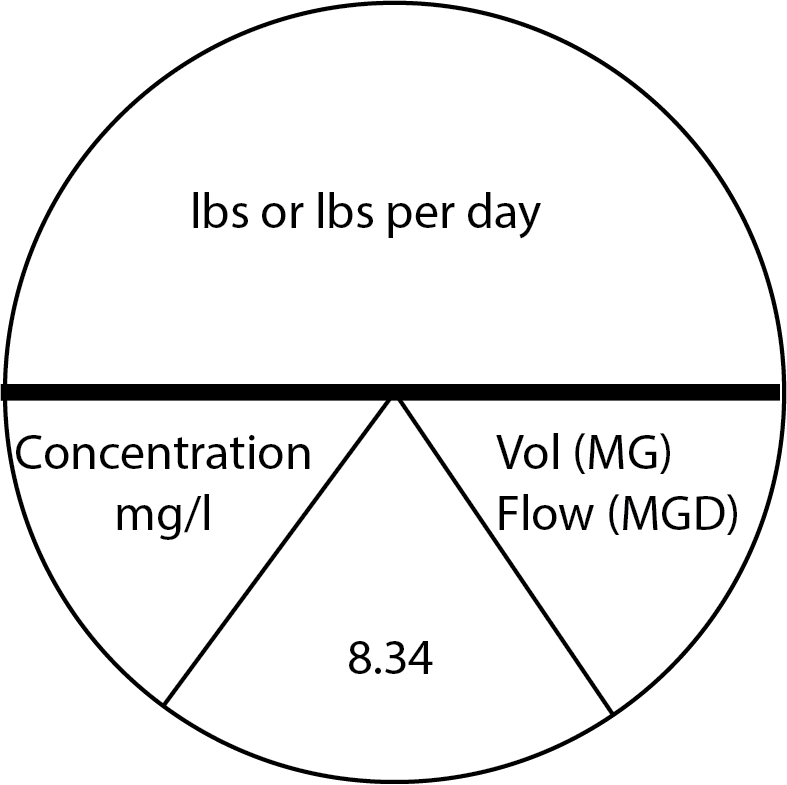
\includegraphics[scale=0.5]{PoundsFormula}
\end{center}

There are three variables – (lbs, concentration and volume) and one constant (8.34) in the pounds formula.  Knowing any of the two variables in the formula, one can calculate the third (unknown) variable by rearranging the equation.

\section{Concentration}\index{Concentration}

Concentration is typically expressed as mg/l which is the weight of the constituent (mg) in 1 l (liter) of solution (wastewater).  As 1 l of water weighs 1 million mg, a concentration of 1 mg/l implies 1 mg of constituent per 1 million mg of water or one part per million (ppm).   \textbf{Thus, mg/l and ppm are synonymous.}\\  
Sometimes the constituent concentration is expressed in terms of percentage.\\
\vspace{6pt}
For example:  sludge containing 5\% solids or a 12.5\% chlorine concentration solution.\\
\vspace{6pt}
As one liter of water weighs 1,000,000 mg, one percent of that weight is 10,000 mg.  So 1\% solids implies 10,000 mg of solids per liter or 10,000 mg/l or 10,000 ppm.\\
\vspace{6pt}
$1\% concentration = 10,000 \enspace ppm \enspace or \enspace\frac{mg}{l}$\\
$0.1\% concentration = 1,000 \enspace ppm \enspace or \enspace \frac{mg}{l}$\\
$0.01\% concentration = 100 \enspace ppm \enspace or \enspace \frac{mg}{l}$\\
$10\% concentration = 100,000 \enspace ppm \enspace or \enspace \frac{mg}{l}$\\
$5\% concentration = 50,000 \enspace ppm \enspace or \enspace \frac{mg}{l}$\\
$12.5\% concentration = 125,000 \enspace ppm \enspace or \enspace \frac{mg}{l}$

\subsection{Example Problems}
% \hl{Example Problems}\\

Problem 1\\Calculate the lbs/day of solids entering the plant given the influent flow is 5 MGD with an average solids concentration  of 250 mg/l.\\

Solution:\\

Applying lbs formula:\\
$\dfrac{lbs}{day}=5 MGD *250\dfrac{mg}{l}*8.34 = \boxed{10,425\dfrac{lbs}{day}}$
\\
Problem 2\\Calculate the lbs of solids in the primary sludge if the sludge flow is 7500 gallons and the solids concentration is 4.5\%.\\
Solution\\
Applying lbs formula:\\
$lbs \enspace solids = \dfrac{7500}{1,000,000}MG * 4.5*10,000 *8.34 = \boxed{2,815 \enspace lbs \enspace solids}$\\
\textbf{Note:}\\  
1) 7500 gallons was converted to MG by dividing by 1,000,000\\
$7500 \enspace gallons * \dfrac{1 MG}{1,000,000 \enspace gallon}$\\
2) 4.5\% was converted to mg/l by multiplying by 10,000 as 1\%=10,000mg/l

\newpage
\section{Area \& Volume}\index{Area \& Volume}
% \section{Area \& Volume}\index{Area \& Volume}

% \begin{snugshade*}
% 	\item \noindent\textsc{Area \& Volume}
% \end{snugshade*}

\begin{center}
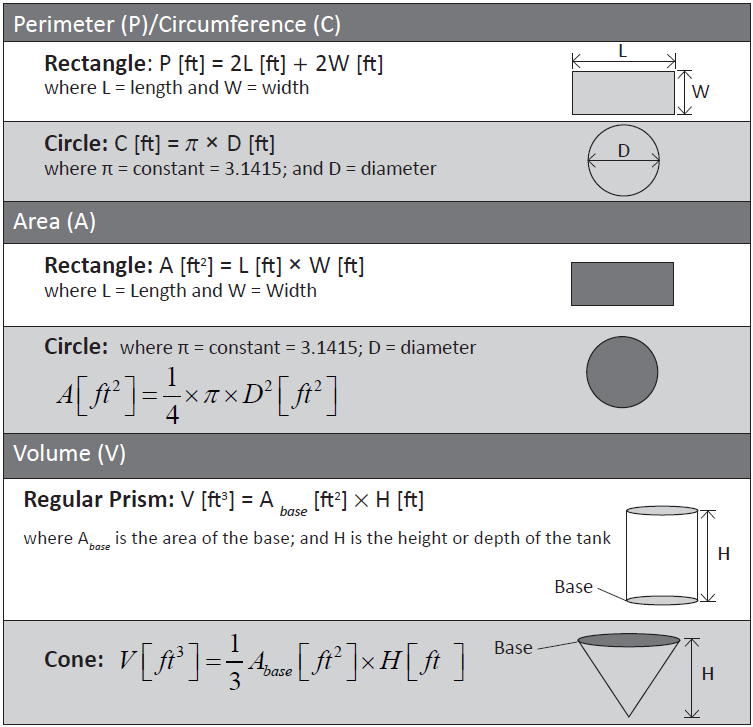
\includegraphics[scale=0.5]{Area&VolumeFormula}
\end{center}
\subsection{Example Problems}
% \hl{Example Problems}\\
\begin{enumerate}

\item The floor of a rectangular building is 20 feet long by 12 feet wide and the inside walls are 10 feet high. Find the total surface area of the inside walls of this building\\
Solution:\\
% \begin{center}
\begin{tikzpicture}
	%%% Edit the following coordinate to change the shape of your
	%%% cuboid
      
	%% Vanishing points for perspective handling
	\coordinate (P1) at (-7cm,1.5cm); % left vanishing point (To pick)
	\coordinate (P2) at (8cm,1.5cm); % right vanishing point (To pick)

	%% (A1) and (A2) defines the 2 central points of the cuboid
	\coordinate (A1) at (0em,0cm); % central top point (To pick)
	\coordinate (A2) at (0em,-2cm); % central bottom point (To pick)

	%% (A3) to (A8) are computed given a unique parameter (or 2) .8
	% You can vary .8 from 0 to 1 to change perspective on left side
	\coordinate (A3) at ($(P1)!.8!(A2)$); % To pick for perspective 
	\coordinate (A4) at ($(P1)!.8!(A1)$);

	% You can vary .8 from 0 to 1 to change perspective on right side
	\coordinate (A7) at ($(P2)!.7!(A2)$);
	\coordinate (A8) at ($(P2)!.7!(A1)$);

	%% Automatically compute the last 2 points with intersections
	\coordinate (A5) at
	  (intersection cs: first line={(A8) -- (P1)},
			    second line={(A4) -- (P2)});
	\coordinate (A6) at
	  (intersection cs: first line={(A7) -- (P1)}, 
			    second line={(A3) -- (P2)});

	%%% Depending of what you want to display, you can comment/edit
	%%% the following lines

	%% Possibly draw back faces

	\fill[gray!40] (A2) -- (A3) -- (A6) -- (A7) -- cycle; % face 6
	\node at (barycentric cs:A2=1,A3=1,A6=1,A7=1) {\tiny Floor=W*L};
	
	\fill[gray!50] (A3) -- (A4) -- (A5) -- (A6) -- cycle; % face 3
	\node at (barycentric cs:A3=1,A4=1,A5=1,A6=1) {\tiny Wall - W*H};
	
	\fill[gray!10, opacity=0.2] (A5) -- (A6) -- (A7) -- (A8) -- cycle; % face 4
	\node at (barycentric cs:A5=1,A6=1,A7=1,A8=1) {\tiny Wall - L*H};
	
	\fill[gray!10,opacity=0.5] (A1) -- (A2) -- (A3) -- (A4) -- cycle; % f2
	\node at (barycentric cs:A1=1,A2=1,A3=1,A4=1) {\tiny Wall - L*H};
	
	\fill[gray!40,opacity=0.2] (A1) -- (A4) -- (A5) -- (A8) -- cycle; % f5
	\node at (barycentric cs:A1=1,A4=1,A5=1,A8=1) {\tiny Ceiling=W*L};	
	
	\draw[thick,dashed] (A5) -- (A6);
	\draw[thick,dashed] (A3) -- (A6);
	\draw[thick,dashed] (A7) -- (A6);

	%% Possibly draw front faces

	%\fill[orange] (A1) -- (A8) -- (A7) -- (A2) -- cycle; % face 1
	\node at (barycentric cs:A1=1,A8=1,A7=1,A2=1) {\tiny Wall - W*H};
	


	%% Possibly draw front lines
	\draw[thick] (A1) -- (A2);

	\draw[<->] (-1.8,0.38) -- (-1.8,-1.3)node [midway, above=-1.8mm] {\hspace{-1.3cm}\tiny Height=10'};
	\draw[<->] (-1.6,-1.4) -- (-.3,-2.1)node [midway, above=-2.6mm] {\hspace{-1.3cm}\tiny Length=20'};
	\draw[<->] (2.6,-1.13) -- (0.2,-2.2)node [midway, below=.6mm] {\hspace{1.2cm}\tiny Width=12'};
	\draw[thick] (A3) -- (A4);
	\draw[thick] (A7) -- (A8);
	\draw[thick] (A1) -- (A4);
	\draw[thick] (A1) -- (A8);
	\draw[thick] (A2) -- (A3);
	\draw[thick] (A2) -- (A7);
	\draw[thick] (A4) -- (A5);
	\draw[thick] (A8) -- (A5);
	
	% Possibly draw points
	% (it can help you understand the cuboid structure)
%	\foreach \i in {1,2,...,8}
%	{
%	  \draw[fill=black] (A\i) circle (0.15em)
%	    node[above right] {\tiny \i};
%	}
	% \draw[fill=black] (P1) circle (0.1em) node[below] {\tiny p1};
	% \draw[fill=black] (P2) circle (0.1em) node[below] {\tiny p2};
\end{tikzpicture}\\
% \end{center}
2 Walls W*H + 2 Walls L*H= $2*12*10ft^2 + 2*20*10ft^2$\\
$=240+400=\boxed{640ft^2}$

2 Walls W*H + 2 Walls L*H + Floor + Ceiling= $2*12*10ft^2 + 2*20*10ft^2 + 2*12*20ft^2$\\
$=240+400+480=\boxed{1,120ft^2}$

\item How many gallons of paint will be required to paint the inside walls of a 40 ft long x 65 ft wide x 20 ft high tank if the paint coverage is 150 sq. ft per gallon.  Note:  We are painting walls only.  Disregard the floor and roof areas.
Solution:\\
\vspace{0.3cm}
% \begin{center}
\begin{tikzpicture}
	%%% Edit the following coordinate to change the shape of your
	%%% cuboid
      
	%% Vanishing points for perspective handling
	\coordinate (P1) at (-7cm,1.5cm); % left vanishing point (To pick)
	\coordinate (P2) at (8cm,1.5cm); % right vanishing point (To pick)

	%% (A1) and (A2) defines the 2 central points of the cuboid
	\coordinate (A1) at (0em,0cm); % central top point (To pick)
	\coordinate (A2) at (0em,-2cm); % central bottom point (To pick)

	%% (A3) to (A8) are computed given a unique parameter (or 2) .8
	% You can vary .8 from 0 to 1 to change perspective on left side
	\coordinate (A3) at ($(P1)!.8!(A2)$); % To pick for perspective 
	\coordinate (A4) at ($(P1)!.8!(A1)$);

	% You can vary .8 from 0 to 1 to change perspective on right side
	\coordinate (A7) at ($(P2)!.7!(A2)$);
	\coordinate (A8) at ($(P2)!.7!(A1)$);

	%% Automatically compute the last 2 points with intersections
	\coordinate (A5) at
	  (intersection cs: first line={(A8) -- (P1)},
			    second line={(A4) -- (P2)});
	\coordinate (A6) at
	  (intersection cs: first line={(A7) -- (P1)}, 
			    second line={(A3) -- (P2)});

	%%% Depending of what you want to display, you can comment/edit
	%%% the following lines

	%% Possibly draw back faces

	\fill[gray!40] (A2) -- (A3) -- (A6) -- (A7) -- cycle; % face 6
	\node at (barycentric cs:A2=1,A3=1,A6=1,A7=1) {};
	
	\fill[gray!50] (A3) -- (A4) -- (A5) -- (A6) -- cycle; % face 3
	\node at (barycentric cs:A3=1,A4=1,A5=1,A6=1) {\tiny Wall - W*H};
	
	\fill[gray!10, opacity=0.2] (A5) -- (A6) -- (A7) -- (A8) -- cycle; % face 4
	\node at (barycentric cs:A5=1,A6=1,A7=1,A8=1) {\tiny Wall - L*H};
	
	\fill[gray!10,opacity=0.5] (A1) -- (A2) -- (A3) -- (A4) -- cycle; % f2
	\node at (barycentric cs:A1=1,A2=1,A3=1,A4=1) {\tiny Wall - L*H};
	
	\fill[gray!40,opacity=0.2] (A1) -- (A4) -- (A5) -- (A8) -- cycle; % f5
	\node at (barycentric cs:A1=1,A4=1,A5=1,A8=1) {};	
	
	\draw[thick,dashed] (A5) -- (A6);
	\draw[thick,dashed] (A3) -- (A6);
	\draw[thick,dashed] (A7) -- (A6);

	%% Possibly draw front faces

	%\fill[orange] (A1) -- (A8) -- (A7) -- (A2) -- cycle; % face 1
	\node at (barycentric cs:A1=1,A8=1,A7=1,A2=1) {\tiny Wall - W*H};
	


	%% Possibly draw front lines
	\draw[thick] (A1) -- (A2);

	\draw[<->] (-1.8,0.38) -- (-1.8,-1.3)node [midway, above=-1.8mm] {\hspace{-1.3cm}\tiny Height=20'};
	\draw[<->] (-1.6,-1.4) -- (-.3,-2.1)node [midway, above=-2.6mm] {\hspace{-1.3cm}\tiny Length=45'};
	\draw[<->] (2.6,-1.13) -- (0.2,-2.2)node [midway, below=.6mm] {\hspace{1.2cm}\tiny Width=65'};
	\draw[thick] (A3) -- (A4);
	\draw[thick] (A7) -- (A8);
	\draw[thick] (A1) -- (A4);
	\draw[thick] (A1) -- (A8);
	\draw[thick] (A2) -- (A3);
	\draw[thick] (A2) -- (A7);
	\draw[thick] (A4) -- (A5);
	\draw[thick] (A8) -- (A5);
	
	% Possibly draw points
	% (it can help you understand the cuboid structure)
%	\foreach \i in {1,2,...,8}
%	{
%	  \draw[fill=black] (A\i) circle (0.15em)
%	    node[above right] {\tiny \i};
%	}
	% \draw[fill=black] (P1) circle (0.1em) node[below] {\tiny p1};
	% \draw[fill=black] (P2) circle (0.1em) node[below] {\tiny p2};
\end{tikzpicture}\\
% \end{center}
\vspace{0.3cm}
2 Walls W*H + 2 Walls L*H = $2*65*20ft^2 + 2*40*20ft^2= 2,600+1,600=4,200ft^2$\\
$\implies @150\dfrac{ft^2}{gal} \enspace paint \enspace coverage \enspace \rightarrow \enspace \dfrac{4,200\cancel{ft^2}}{150\dfrac{\cancel{ft^2}}{gal}}=\boxed{28 \enspace gallons}$
\vspace{0.3cm}
\item What is the circumference of a 100 ft diameter circular clarifier?\\
\vspace{0.3cm}
Solution:\\
\vspace{0.3cm}
$Circumference=\pi*D=3.14*100ft=\boxed{314ft}$
\vspace{0.3cm}
\item If the surface area of a clarifier is 5,025$ft^2$, what is its diameter?\\
\vspace{0.3cm}
Solution:\\
\vspace{0.3cm}
$Surface \enspace area=\dfrac{\pi}{4}*D^2 \enspace \implies 5025(ft^2)=0.785*D^2 (ft^2)$\\
$\implies D^2=\dfrac{5025}{0.785} \implies D=\sqrt{6401.3}=\boxed{80ft}$
\vspace{0.3cm}

\item How many gallons of wastewater would 600 feet of 6-inch diameter pipe hold, approximately?\\
\vspace{0.3cm}
Solution:\\

\vspace{0.3cm}
% \begin{center}
\begin{tikzpicture}
\draw (0,0) ellipse (0.1cm and 0.3cm);
\draw (10,0) ellipse (0.1cm and 0.3cm);
\draw [-] (0,-0.29) -- (10,-0.29);
\draw [-] (0,0.29) -- (10,0.29);
\draw [<->] (10,-0.28) -- (10,0.28) node [midway, below=-3mm] {\hspace{2.6cm}Diameter=6"};
\draw [<->] (0,-.68) -- (10,-.68)node [midway, below] {\hspace{0.9cm}Length=600'};
\end{tikzpicture}
% \end{center}
\vspace{0.3cm}
$Volume=\dfrac{\pi}{4}D^2*L=0.785*\Big(\dfrac{6}{12}\Big)^2*600\cancel{ft^3}*7.48\dfrac{gallons}{\cancel{ft^3}}=\boxed{881 \enspace gallons}$
\newpage
\item A 110 ft diameter digester with a 12 ft deep cone is operated at a side water depth of 20 ft.  Caluclate the volume of sludge in the digester in $ft^3$ and gallons.\\
\vspace{0.3cm}
Solution:\\
\vspace{0.3cm}
% \begin{center}
\begin{tikzpicture}
\draw (0,0) ellipse (2cm and 0.3cm);
\draw (0,-2.3) ellipse (2cm and 0.3cm);
\draw (0,-.8) ellipse (2cm and 0.3cm);
\draw [-] (2,-2.3) -- (2,0);
\draw [<->] (-2,0) -- (2,0) node [midway, below=-0.9cm] {\hspace{0.9cm}Diameter (D)=110'}; 
\draw [<->] (-2.6,-2.3) -- (-2.6,0) node [midway, below=-.3cm] {\hspace{-2.6cm}Cylinder Height};
\draw [<->] (2.5,-2.3) -- (2.5,-0.8) node [midway, below=-0.2cm] {\hspace{5.2cm}Side Water Depth (SWD) =20'};
\draw [-] (0,-4) -- (2,-2.3);
\draw [-] (0,-4) -- (-2,-2.3);
\draw [-] (0,-4) -- (2,-2.3);
\draw [-] (-2,0) -- (-2,-2.3);
\draw [<->] (2.5,-2.3) -- (2.5,-4)node [midway, below=-0.4cm] {\hspace{3.8cm}Cone Depth (CD)=12'};
\end{tikzpicture}\\
% \end{center}
$Digester \enspace volume=Volume_{cylinder}+Volume_{cone}$\\
$\implies Digester \enspace volume=\dfrac{\pi}{4}D^2*SWD+\dfrac{1}{3}*\Bigg(\dfrac{\pi}{4}*D^2*CD\Bigg)$\\
\vspace{0.3cm}
$=0.785*110^2*20+1.05*110^2*12=\boxed{227,988ft^3}$\\
\vspace{0.3cm}
$227,988\cancel{ft^3}*7.48\dfrac{gallons}{\cancel{ft^3}}=\boxed{1,705,352 \enspace gallons}$
\end{enumerate}

\section{Process Removal Efficiency}\index{Process Removal Efficiency}

% \section{Process Removal Efficiency}\index{Process Removal Efficiency}
% \begin{snugshade*}
% 	\item \noindent\textsc{Process Removal Efficiency}
% \end{snugshade*}
\begin{itemize}
\item Process removal rate or removal efficiency is the percentage of the inlet concentration removed.  
\item It is used for quantifying the pollutant removal during wastewater treatment and is established based upon the amount of a particular wastewater constituent entering and leaving a treatment process.

\item $Process \enspace Removal \enspace Rate \enspace (\%) = \dfrac{Pollutant \enspace  In-Pollutant\enspace  Out}{Pollutant \enspace In}*100$\\

\item If 10 units of a pollutant are entering a process and 8 units of pollutant are leaving (process removes 2 units), then the process removal rate for that pollutant is (10-8)/10*100=20\%.  In this example the process is 20\% efficient in removing that particular pollutant.

\item The amount of pollutant can be measured in terms of concentration (mg/l) or in terms of mass loading (lbs).  The pounds formula is used for calculating the mass loadings.  
\end{itemize}
The above example is for calculating the removal efficiency using the inlet and outlet concentrations or mass loading.\\
The methods below can be used for calculating either the inlet or outlet pollutant concentrations, if the removal efficiency and the corresponding inlet or outlet concentrations are given. 


\hl{Case 1:  Calculating outlet conc. (X) given the inlet conc. and removal efficiency (RE\%):}

\tikzstyle{block} = [rectangle, draw, fill=red!40, 
    text width=6em, text centered, rounded corners, minimum height=3em]
\tikzstyle{arrow} = [draw, -latex']
\begin{figure}[!h]
\centering
\begin{tikzpicture}[node distance =1.5cm, auto]
    \draw ++(0,0) node [block] (Process) {Process};
   \node[node distance=1.9in] (dummy_in) [left of=Process] {In};
   \node[node distance=1.9in] (dummy_out) [right of=Process] {Out};
	\node (Removal) [below of=Process, yshift=-0in] {${Removal \enspace Efficiency=RE\% \enspace (Given)}$};
    \path [arrow] (dummy_in)-- (Process)  node [above] {\hspace{-5.8cm}$A \enspace mg/l \enspace (Given) $} node [below] {\hspace{-5.8cm}$100 \enspace mg/l$};
    \path [arrow] (Process) -- (dummy_out)  node [above] {\hspace{-4cm}$X \enspace mg/l \enspace (Unknown)$} node [below] {\hspace{-3.9cm}($100-RE\%)\enspace mg/l$};
   \draw[arrow] (Process) -- (Removal);
\end{tikzpicture}
\end{figure}
Using the fact that if the inlet concentration was 100 mg/l, the outlet concentration would be 100 minus the removal efficiency.\\
Setup the equation as:  $\dfrac{Out}{In}: \enspace \dfrac{X \enspace mg/l}{A \enspace mg/l}=\dfrac{100-RE\%}{100}$\\
Calculate X using cross multiplication - if $\dfrac{A}{B}=\dfrac{C}{D} \implies A=B*\dfrac{C}{D}$:\\
$X \enspace mg/l=A \enspace mg/l*\dfrac{100-RE\%}{100}$\\


\hl{Case 2:  Calculating inlet conc. (X) given the outlet conc. and removal efficiency (RE\%):}

\begin{figure}[!h]
\centering
\begin{tikzpicture}[node distance =1.5cm, auto]
    \draw ++(0,0) node [block] (Process) {Process};
   \node[node distance=1.9in] (dummy_in) [left of=Process] {In};
   \node[node distance=1.9in] (dummy_out) [right of=Process] {Out};
	\node (Removal) [below of=Process, yshift=-0in] {$Removal \enspace Efficiency=RE\% \enspace (Given)$};
    \path [arrow] (dummy_in)-- (Process)  node [above] {\hspace{-5.8cm}$X \enspace mg/l \enspace (Unknown)$} node [below] {\hspace{-5.8cm}$100 \enspace mg/l$};
    \path [arrow] (Process) -- (dummy_out)  node [above] {\hspace{-4cm}$A \enspace mg/l \enspace (Given)$} node [below] {\hspace{-3.9cm}($100-RE\%)\enspace mg/l$};
   \draw[arrow] (Process) -- (Removal);
\end{tikzpicture}
\end{figure}
Using the fact that if the inlet concentration was 100 mg/l, the outlet concentration would be 100 minus the removal efficiency.\\
Setup the equation as:  $\dfrac{In}{Out}: \enspace \dfrac{X \enspace mg/l}{A \enspace mg/l}=\dfrac{100}{100-RE\%}$\\
\vspace{0.3cm}
Calculate X using cross multiplication - if $\dfrac{A}{B}=\dfrac{C}{D} \implies A=B*\dfrac{C}{D}$:\\
$X \enspace mg/l=A \enspace mg/l*\dfrac{100}{100-RE\%}$\\

\vspace{0.4cm}
\subsection{Example Problems}
% \hl{Example Problems:}\\

\begin{enumerate}

\item What is the \% removal efficiency if the influent concentration is 10 mg/L and the effluent concentration is 2.5 mg/L?\\
$Removal \enspace Rate (\%) = \dfrac{In-Out}{In}*100 \implies \dfrac{10-2.5}{10}*100=\boxed{75\%}$



\item Calculate the outlet concentration if the inlet concentration is 80 mg/l and the process removal efficiency is 60\%\\
Solution:\\

\tikzstyle{block} = [rectangle, draw, fill=red!40, 
    text width=6em, text centered, rounded corners, minimum height=3em]
\tikzstyle{arrow} = [draw, -latex']
\begin{figure}[!h]
\centering
\begin{tikzpicture}[node distance =1.5cm, auto]
    \draw ++(0,0) node [block] (Process) {Process};
   \node[node distance=1.5in] (dummy_in) [left of=Process] {In};
   \node[node distance=1.5in] (dummy_out) [right of=Process] {Out};
	\node (Removal) [below of=Process, yshift=-0in] {$Removal \enspace Efficiency=60\%$};
    \path [arrow] (dummy_in)-- (Process)  node [above] {\hspace{-4.39cm}$80mg/l$} node [below] {\hspace{-4.39cm}$100mg/l$};
    \path [arrow] (Process) -- (dummy_out)  node [above] {\hspace{-3.cm}$Xmg/l$} node [below] {\hspace{-3cm}40mg/l};
   \draw[arrow] (Process) -- (Removal);
\end{tikzpicture}
%\caption[MFCC]{Diagrama en bloques del cálculo de las MFCC para un frame.}
%\label{MFCC}
\end{figure}

$\dfrac{Out}{In} \enspace:\enspace\dfrac{Actual \enspace Outlet (X)}{80}=\dfrac{100-60}{100}$\\
$\implies \dfrac{Actual \enspace Outlet (X)}{80} =0.4$\\
$\implies Actual \enspace  Outlet (X) = 0.4 * 80 = \boxed{32 mg/l}$\\


\item Calculate the inlet concentration if the outlet concentration is 80 mg/l and the process removal efficiency is 60\%\\

\tikzstyle{block} = [rectangle, draw, fill=red!40, 
    text width=6em, text centered, rounded corners, minimum height=3em]
\tikzstyle{arrow} = [draw, -latex']
\begin{figure}[!h]
\centering
\begin{tikzpicture}[node distance =1.5cm, auto]
    \draw ++(0,0) node [block] (Process) {Process};
   \node[node distance=1.5in] (dummy_in) [left of=Process] {In};
   \node[node distance=1.5in] (dummy_out) [right of=Process] {Out};
	\node (Removal) [below of=Process, yshift=-0in] {$Removal \enspace Efficiency=60\%$};
    \path [arrow] (dummy_in)-- (Process)  node [above] {\hspace{-4.39cm}$Xmg/l$} node [below] {\hspace{-4.39cm}$100mg/l$};
    \path [arrow] (Process) -- (dummy_out)  node [above] {\hspace{-3.cm}80mg/l} node [below] {\hspace{-3cm}40mg/l};
   \draw[arrow] (Process) -- (Removal);
\end{tikzpicture}
\end{figure}

$\dfrac{In}{Out} \enspace : \enspace \dfrac{Actual \enspace inlet \enspace  (X)}{80}=\dfrac{100}{100-60}\implies \dfrac{Actual \enspace inlet \enspace  (X)}{80}=2.5$\\    
Rearranging the equation:   $Actual \enspace inlet (X)=2.5*80 = \boxed{200 mg/l}$\\

\item If a plant removes 35\% of the influent BOD in the primary treatment and 85\% of the remaining BOD in the secondary system, what is the BOD of the raw wastewater if the BOD of the final effluent is 20mg/l\\
Solution:\\

\begin{figure}[!h]
\centering
\begin{tikzpicture}[node distance =1.5cm, auto]
    \draw ++(0,0) node [block] (Primary) {Primary};
    
   \node[node distance=1.9in] (dummy_in) [left of=Primary] {Influent BOD};
   \node[node distance=1.9in] (dummy_out) [right of=Primary] {Primary BOD Out};
	\node (Removal) [below of=Primary, yshift=-0in] {$Removal \enspace Efficiency=35\% $};
    \path [arrow] (dummy_in)-- (Primary)  node [above] {\hspace{-4.8cm}$X \enspace mg/l \enspace$} node [below] {};
    \path [arrow] (Primary) -- (dummy_out)  node [above] {\hspace{-4.9cm}$0.65X \enspace mg/l$} node [below] {};
   \draw[arrow] (Process) -- (Removal);
\end{tikzpicture}
\end{figure}


\begin{figure}[!h]
\centering
\begin{tikzpicture}[node distance =1.5cm, auto]
    \draw ++(0,0) node [block] (Secondary) {Secondary};
    
   \node[node distance=1.9in] (dummy_in) [left of=Secondary] {Primary BOD Out};
   \node[node distance=1.9in] (dummy_out) [right of=Secondary] {Secondary BOD Out};
	\node (Removal) [below of=Secondary, yshift=-0in] {$Removal \enspace Efficiency=85\% $};
    \path [arrow] (dummy_in)-- (Secondary)  node [above] {\hspace{-4.8cm}$0.65X \enspace mg/l \enspace$} node [below] {\hspace{-5cm}$100 \enspace mg/l$};
    \path [arrow] (Secondary) -- (dummy_out)  node [above] {\hspace{-4.9cm}$20 \enspace mg/l$} node [below] {\hspace{-4.9cm}$15 \enspace mg/l$};
   \draw[arrow] (Process) -- (Removal);
\end{tikzpicture}
\end{figure}
\vspace{0.3cm}
For the Secondary process:\\
$\dfrac{In}{Out}: \enspace \dfrac{0.65X}{20}=\dfrac{100}{15} \implies X \enspace mg/l=\dfrac{100*20}{15*0.65}=\boxed{205 \enspace mg/l}$\\

\vspace{0.3cm}
Alternate Solution \#1

$\xrightarrow[
				\text{X}\dfrac{mg}{l}
			]
			{
			\text{Influent BOD}
			}
 \boxed{Primary}
 \xrightarrow[
 				\text{X-0.35X=X*(1-0.35)=0.65X}\dfrac{mg}{l}
 			]
 			{
 			\text{Primary Effluent BOD}
 			}
 \boxed{Secondary}
 \xrightarrow[
				\text{0.65X-0.5525X=(0.65-0.5525)X=0.0975X }
			 ]
			{
			\text{Secondary Effluent BOD}
			}
$\\
\hspace{2.8cm}$\downarrow$ {\tiny(0.35X)BOD Removed}\hspace{3.2cm}$\downarrow$ {\tiny(0.65*0.85)X = 0.5525X BOD Removed}\\
$\implies 0.0975X=20 \implies X=\dfrac{20}{0.0975}=\boxed{205\dfrac{mg}{l}}$\\

\vspace{0.3cm}

Alternate Solution \#2:\\
$\xrightarrow[\text{X}\dfrac{mg}{l}]{\text{Influent BOD}}\boxed{Primary}\xrightarrow[\text{0.65X}]{\text{Primary Effluent BOD}}\boxed{Secondary}\xrightarrow[\text{(0.65*0.15)X}]{\text{Secondary Effluent BOD}}$\\
\hspace{2.8cm}$\downarrow$ {\tiny(0.35X)BOD Removed}\hspace{2.2cm}$\downarrow$ {\tiny(0.65X*0.85)BOD Removed}\\

Primary Effluent BOD = Influent BOD * (1-Primary BOD Removal), and\\
Secondary Effluent BOD=[Primary Effluent BOD]*(1-Secondary BOD Removal)\\
Secondary Eff. BOD=[Influent BOD * (1-Primary BOD Removal)]*(1-Secondary BOD Removal)\\

Therefore, 20 = [X*(1-0.35)] * (1-0.85)= X*0.65*0.15\\
$\implies 20 \enspace \dfrac{mg}{l}= 0.0975X \implies X=\dfrac{20}{0.0975}=\boxed{205 \enspace \dfrac{mg}{l}}$

\end{enumerate}
\section{Pumping}\index{Pumping}
% \section{Pumping}\index{Pumping}
% \pagebreak
% \begin{snugshade*}
% 	\item \noindent\textsc{Pumping}
% \end{snugshade*}
For Grades I \& II, pumping rate problems include the following:
% \begin{enumerate}
% \definecolor{shadecolor}{RGB}{225, 235, 235}
% \begin{snugshade*}
% \item \noindent\textsc{Calculating volume pumped in a given time interval given the pump flow rate\\}
% \end{snugshade*}
\subsection{Calculating volume pumped given the pump flow rate}\index{Calculating volume pumped given the pump flow rate}

\textbf{Method:\\}
\hspace{1cm}Step 1. Multiply the pump flow rate by the time interval\\
\textbf{Make sure:}
\begin{itemize}
\item The time units - in the given time interval and in the pump flow rate match
\end{itemize}
\subsection{Calculating time to pump a certain volume}\index{Calculating time to pump a certain volume}
% \begin{snugshade*}
% \item \noindent\textsc{Calculating time to pump a certain volume given the pump flow rate\\}
% \end{snugshade*}
\textbf{Method:}
\hspace{1cm}Step 1. Calculate the total volume pumped\\
\hspace{1cm}Step 2.	Divide the total volume by the pump flow rate\\
\textbf{Make sure:}
\begin{itemize}
\item The volume units - in the volume that needs to be pumped and in the pump flow rate match
\item The time unit in the pump flow rate needs to be converted to the time unit that you need the answer in
\end{itemize}
% \end{enumerate}

\section{Example Problems}
% \hl{Example Problems:}\\

\begin{enumerate}

\item A sludge pump is set to pump 5 minutes each hour. It pumps at the rate of 35 gpm. How many gallons of sludge are pumped each day?\\
Solution:\\
$\dfrac{35 \enspace gal \enspace sludge}{\cancel{min}}*\dfrac{5 \enspace \cancel{min}}{\cancel{hr}} *\dfrac{24 \enspace \cancel{hr}}{day}=\boxed{\dfrac{4,200 \enspace gallons}{day}}$\\
\vspace{0.5cm}

\item A sludge pump operates 5 minutes each 15 minute interval.  If the pump capacity is 60 gpm, how many gallons of sludge are pumped daily?

$\dfrac{60 \enspace gal \enspace sludge}{\xcancel{min}}*\dfrac{5 \enspace \xcancel{min}}{15 \enspace \cancel{min}}*1440\dfrac{\cancel{min}}{day}=\boxed{\dfrac {28,800 \enspace gal \enspace sludge }{day}}$\\

\item Given the tank is 10ft wide, 12 ft long and 18 ft deep tank including 2 ft of freeboard when filled to capacity. How much time (minutes) will be required to pump down this tank to a depth of 2 ft when the tank is at maximum capacity using a 600 GPM pump\\
Solution:\\
\vspace{0.5cm}


\begin{tikzpicture}

\pgfmathsetmacro{\cubexx}{4}
\pgfmathsetmacro{\cubeyy}{1.5}
\pgfmathsetmacro{\cubezz}{2}
\pgfmathsetmacro{\cubex}{4}
\pgfmathsetmacro{\cubey}{0.5}
\pgfmathsetmacro{\cubez}{2}
\pgfmathsetmacro{\cubexxx}{4}
\pgfmathsetmacro{\cubeyyy}{4}
\filldraw [fill=cyan!10!white, draw=black] (0,-\cubey,0) -- ++(-\cubexx,0,0) -- ++(0,-\cubeyy,0) -- ++(\cubexx,0,0) -- cycle ;
\filldraw [fill=cyan!0!white, draw=black] (0,-\cubey,0) -- ++(0,0,-\cubezz) -- ++(0,-\cubeyy,0) -- ++(0,0,\cubezz) -- cycle;
\filldraw [fill=cyan!10!white, draw=black] (0,-\cubey,0) -- ++(0,0,-\cubezz) -- ++(0,-\cubeyy,0) -- ++(0,0,\cubezz) -- cycle;
%\filldraw [fill=cyan!10!white, draw=black] (0,-\cubey,0) -- ++(-\cubexx,0,0) -- ++(0,0,-\cubezz) -- ++(\cubexx,0,0) -- cycle;
%%%\draw (0,-0.5,0) -- ++(-\cubex,0,0) -- ++(0,-\cubey,-\cubez) -- ++(\cubex,0,0) -- cycle;
\draw (-\cubex,0,0) -- ++(0,0,-\cubez) -- ++(0,-\cubey,0) -- ++(0,0,\cubez) -- cycle;
\draw (0,-\cubey,0) -- ++(-\cubex,0,0) -- ++(0,0,-\cubez) -- ++(\cubex,0,0) -- cycle;
\filldraw [fill=white, draw=black] (0,0,0) -- ++(-\cubex,0,0) -- ++(0,-\cubey,0) -- ++(\cubex,0,0) -- cycle ;
\filldraw [fill=white, draw=black] (0,0,0) -- ++(0,0,-\cubez) -- ++(0,-\cubey,0) -- ++(0,0,\cubez) -- cycle;
\filldraw [fill=white, draw=black] (0,0,0) -- ++(0,0,-\cubez) -- ++(0,-\cubey,0) -- ++(0,0,\cubez) -- cycle;
\filldraw [fill=white, draw=black] (0,0,0) -- ++(-\cubex,0,0) -- ++(0,0,-\cubez) -- ++(\cubex,0,0) -- cycle;

%\filldraw [fill=RoyalBlue!10!white, draw=black] (0,-1.5,0) -- ++(-\cubex,0,0) -- ++(0,-\cubey,0) -- ++(\cubex,0,0) -- cycle ;

%\filldraw [fill=RoyalBlue!10!white, draw=black] (0,-1.5,0) -- ++(0,0,-\cubez) -- ++(0,-\cubey,0) -- ++(0,0,\cubez) -- cycle;



%%\draw (0,-0.5,0) -- ++(-\cubex,0,0) -- ++(0,0,-\cubez) -- ++(\cubex,0,0) -- cycle;
%%\filldraw [fill=white, draw=black] (-\cubex,0,0) -- ++(0,0,-\cubez) -- ++(0,-\cubey,0) -- ++(0,0,\cubez) -- cycle;
%%\filldraw [fill=white, draw=black] (0,-\cubey,0) -- ++(-\cubex,0,0) -- ++(0,0,-\cubez) -- ++(\cubex,0,0) -- cycle ;

\draw [<->] (-4,-2.3) -- (0,-2.3) node [midway, below] {12' Long};
\draw [<->] (1,-1.3) -- (1,.2) node [midway, midway] {\hspace{4.5cm}16' Water Depth (Initial)};
\draw [<->] (0.4,-1.62) -- (0.4,-1.1) node [midway, midway] {\hspace{-4.8cm} 2' Water Depth (Final)};
\draw [<->] (1,.8) -- (1,.2) node [midway, midway] {\hspace{2.4cm}2' Freeboard};
\draw [<->] (1,-1.3) -- (0,-2.3) node [midway, midway] {\hspace{2.3cm}10' Wide};
\end{tikzpicture}\\
Volume to be pumped=$12 \enspace ft*10 \enspace ft *(16-2)\enspace ft=1,680ft^3$\\
\vspace{0.3cm}
$\implies \dfrac{1,680\cancel{ft^3}*7.48\dfrac{\cancel{gal}}{\cancel{ft^3}}}{600\dfrac{\cancel{gal}}{min}}=\boxed{21min}$
\end{enumerate}

\chapterimage{TitleIII.png} % Chapter heading image

\chapter{Wastewater Constituents and Analysis}
% \begin{enumerate}[1.]
% 	\definecolor{shadecolor}{RGB}{200, 200, 240}

% 	%%%%%%%%%%%
% 	% LEVEL 2 %
% 	%%%%%%%%%%%

% 	\begin{snugshade*}
% 		\item \noindent\textsc{Wastewater Constituents}%$$$$$$$$$$$$$$$$$$$$%
% 	\end{snugshade*}
% 	Solids, organic matter, nutrients, pathogens and oil \& grease are the main target constituents of wastewater treatment operations.
% 	\begin{enumerate}[A.]%___________%
% 			\definecolor{shadecolor}{RGB}{225, 235, 235}

				%%%%%%%%%%%
				% LEVEL 3 %
				%%%%%%%%%%%
		% \begin{snugshade*}
		% 	\item \noindent\textsc{Organic Matter}%###############################%
		% \end{snugshade*}
		
		\section{Organics}\index{Organics}		
		\begin{itemize}
			\item The main reason for treating domestic wastewater is to remove the organic matter.  
			\item Organics are substances containing carbon, hydrogen and oxygen, and some of which may be combined with nitrogen, sulfur or phosphorous.
			\item About 50 percent of the solids present in wastewater are organic.  This fraction is generally of animal or vegetable life, dead animal matter, plant tissue or organisms, and also include synthetic organic compounds.
			\item The principal organic compounds present in domestic wastewater are proteins, carbohydrates and fats together with the products of their decomposition.
			\item Organics are subject to decay or decomposition through the activity of bacteria and other living organisms.  \hl{Since the organic fraction can be driven off at high temperatures, they are also called \textbf{volatile solids}}.\
			\item \emph{Organics in wastewater is typically quantified in terms of oxygen required to oxidize the carbon based material present} in wastewater using the following methods:\\
\subsection{Biochemical Oxygen Demand (BOD)}\index{Biochemical Oxygen Demand (BOD)}

			  %     \begin{enumerate}[i.]
			  %     	\definecolor{shadecolor}{RGB}{220,220,220}
					% %%%%%%%%%%%
					% % LEVEL 4 %
					% %%%%%%%%%%%
			  %     	\begin{snugshade*}
			  %     		\item \noindent\textsc{Biochemical Oxygen Demand (BOD)}%@@@@@@@@@@@@@@@@@@%
			  %     	\end{snugshade*}					
			      	\begin{itemize}
			      		\item The BOD of wastewater is measured in terms of oxygen required for the microorganisms to consume the organic material present.
			      		\item BOD is typically measured as BOD$_5$ which is the oxygen demand of the wastewater measured after 5 days of the initiation of the test.
			      		\item The test involves incubating a known dilution of wastewater in a 300 ml bottle for 5 days at 20\si{\degree}C.  The dissolved oxygen (DO) content at the start and end of the incubation period is used for calculating the BOD.
			      		\item For the test to be considered valid, the following criteria need to be met: 1) DO consumption during the test must be at least 2 mg/l, 2) DO remaining at the end of the test must be at least 1 mg/l, and 3) DO consumed in blank should be 0.2 mg/l or less
			      		      			
			      		\item BOD is a parameter to measure the strength of wastewater and the measurement of the wastewater treatment plant or treatment process influent and effluent BOD is standard practice to measure its performance.  Typical domestic wastewater BOD is about 200-250 mg/l.
			      		\item The oxygen consumed by the microorganisms during the BOD test is primarily for: 1) Oxidizing the carbonaceous material (cBOD – carbonaceous BOD), and 2) Oxidizing nitrogenous constituents such as ammonia (nBOD – nitrogenous BOD).
			      		\item Thus, BOD (Total) = cBOD + nBOD.  The cBOD and nBOD is measured by adding certain chemical inhibitors which will inhibit the bacteria responsible for consuming the nitrogenous matter, thus measuring only the cBOD as part of the BOD test.
			      		\item Since not all of the organics is metabolized in the 5 days of the regular BOD test, certain wastewater discharge permits require reporting of the ultimate BOD value (BOD$_U$)\\
			      	\end{itemize}

			    \subsection{Chemical Oxygen Demand (COD)}\index{Chemical Oxygen Demand (COD)}
			      	% \begin{snugshade*}
			      	% 	\item \noindent\textsc{Chemical Oxygen Demand (COD)}%@@@@@@@@@@@@@@@@@@%
			      	% \end{snugshade*}		  
			      	\begin{itemize}
			      		\item The COD test involves using chemical oxidizers to measure the oxygen demand of the wastewater.
			      		\item As the chemical oxidizers will oxidize other constituents present, including inorganic matter, the COD value of wastewater will be higher than the BOD.  
			      		\item The COD test can be conducted rather quickly than the 5 day BOD test, it is an effective method to quantify the wastewater strength and process efficiencies and allow operators to make timely process adjustments.
			      	\end{itemize}

			    \subsection{Total Organic Carbon (TOC)}
			      	% \begin{snugshade*}
			      	% 	\item \noindent\textsc{Total Organic Carbon (TOC):}\\%@@@@@@@@@@@@@@@@@@%
			      	% \end{snugshade*}
			      	The TOC method utilizes laboratory analytical instruments which directly measure the organic carbon content by quantifying the amount of carbon dioxide produced from the complete combustion of the organics present.
			      % \end{enumerate}
		\end{itemize}
		
		
		
			\hl{Note: BOD measures the amount of oxygen required by the microorganisms present to consume the organic material while COD measures the chemical oxidation required to oxidize all chemicals including organics present in wastewater.  BOD value of typical domestic sewage is about 200 - 250 mg/l while the COD value ranges from 300 - 450 mg/l.  Typical BOD:COD ratio ranges from 0.5-0.8.}\\


\section{Solids}\index{Solids}
% 		\pagebreak
% 				\begin{snugshade*}
% 			\item \noindent\textsc{Solids}
% 		\end{snugshade*}	
		Like BOD, wastewater solids is another critical parameter for establishing the wastewater strength and determining treatment process efficiencies. 
		\begin{itemize}
			\item The \texthl{solids can be classified as suspended or dissolved} based upon its ability to pass through a standardized filter paper.
			\item When the wastewater is filtered:
			      \begin{itemize}
			      	\item the residual solids remaining on the filter paper after drying in an oven at 103\si{\degree}C is the \hl{suspended solids} portion, and 
			      	\item the solids remaining after drying the filtrate are the \hl{dissolved solids}.
			      \end{itemize}
			\item Suspended solids include larger floating particles and consist of sand, grit, clay, fecal matter, paper, pieces of wood, particles of food and garbage, and similar materials.
			\item Suspended solids can be categorized based upon its settling characteristics as:
			      \begin{itemize}
			      	\item \hl{Settleable}
			      	\item \hl{Non-settleable}
			      	      \begin{itemize}
			      	      	\item \hl{Colloidial}-small, charged (typically negative) particles which do not settle easily.  Some of the colloidial particles are small enough to pass through the filter paper used for filtering the suspended solids
			      	      	\item \hl{Floatable}-example oil and grease and small plastics
			      	      \end{itemize}
			      \end{itemize}
			\item Dissolved solids in wastewater include organics.  However, the major elements of dissolved solids are inorganic ions such as Ca$^{+2}$, Mg$^{+2}$, Cl$^-$, SO$_4$ $^{-2}$ , HCO$_3$ $^-$, Fe$^{+2}$, PO$_4$ $^{-3}$, NO$_3$ $^-$.  These ions are part of the dissolved salts such as sodium chloride (NaCl), calcium bicarbonate (Ca(HCO$_3$)$_2$), magnesium phosphate (Mg$_3$PO$_4$) and others which are normally present in water and wastewater. 
			      \begin{itemize}
			      	\item Conductivity or electrical conductance (EC) measurement is typically conducted as the wastewater enters the plant as \hl{conductivity provides an indirect and simple measure of the amount of dissolved solids present.}  
			      	\item Conductivity or electrical conductance (EC) is a measure the amount of electrical current that can be conducted by a solution.  
			      	\item The conductance of electricity in a solution is due to the presence of dissolved inorganic ions 
			      	\item The higher the concentration of these ions, the higher is the conductivity. 
			      	\item \underline{Conductivity is measured in the units of mhos/cm or Siemens/cm.}  (Note:  mhos is the reverse of ohm which is a measure of resistance).
			      	\item Typical wastewater conductivities range from 50 to 1500 S/cm
			      \end{itemize}
			\item Both suspended and dissolved solids can be either \hl{volatile (organic)} or \hl{fixed (inorganic)}.
			\item \hl{Total Solids is thus a sum of TSS and dissolved solids or volatile and fixed solids.}
			      \begin{itemize}
			      	\item The volatile solids are typically of plant or animal origin .
			      	\item The fixed solids include sand, gravel and silt as well as the dissolved salts.
			      \end{itemize}
			      \begin{minipage}{0.5\textwidth}
			      	\item The volatile or fixed fractions are quantified by incinerating the solids in a muffler furnace at 550\si{\degree} which removes only the volatile solids leaving only the fixed solids behind.
			      	\item In terms of the size of the solids, the distribution is approximately thirty percent suspended and about seventy percent dissolved solids - which includes the colloidal particles which have passed through the filter paper.\\ 
			      	\item As primary treatment process involve settling of solids, establishing the settleable portion of the suspended solids is important.\\  
			      	\item \hl{The settleable solids are quantified using an Imhoff cone and are reported in ml/L}.  Imhoff cone is a 1 liter, clear cone shaped container, with volume graduations (ml) at the bottom.
			      						
			      \end{minipage}	
			      \begin{minipage}{0.5\textwidth}
			      	\begin{center}
			      		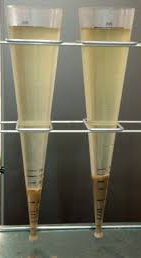
\includegraphics[scale=0.7]{ImhoffCone}\\
			      		Imhoff Cone\\
			      		\textit{Note the ml markings at the bottom of the cone}
			      		
			      		
			      	\end{center}
		      \end{minipage}
%			      \end{minipage}
			      	\item One factor which affects settleability is the conveyance time of the sewage to the treatment plant. 			
			      	\item The settleable component of the suspended solids will decrease as the sewage becomes more septic due to longer conveyance times.
			\item Influent and effluent total suspended solids are measured to establish the overall treatment and individual process efficiencies.  
			\item Volatile solids measurements before and after biological processes such as secondary treatment and digestion provide information on the process efficiency.\\
		\end{itemize}


	\subsection{Procedures for Solids Analysis}\index{Procedures for Solids Analysis}
% 		\begin{enumerate}%$$$$$$$$$$$$$$$$$$$$%
% 			\definecolor{shadecolor}{RGB}{220, 220, 220}
% 			\begin{snugshade*}
% 				\item \noindent\textsc{Procedures for Solids Analysis}
% 			\end{snugshade*}		
	\subsubsection{Determining wastewater suspended solids - Total(TSS) and Volatile(VSS) concentrations}\index{Determining wastewater suspended solids - Total(TSS) and Volatile(VSS) concentrations}			
			% \begin{enumerate}[a.]
			% 	\definecolor{shadecolor}{RGB}{110, 192, 221}
			% 	\begin{snugshade*}
			% 		\item \noindent\textsc{Determining wastewater suspended solids - Total(TSS) and Volatile(VSS) concentrations:}
			% 	\end{snugshade*}
				 
				%\hl{How total suspended solids concentration is established for a wastewater sample:}
				\begin{itemize}
					\item A known volume of wastewater sample is filtered through a pre-weighed filter paper
					\item The suspended solids will be retained by the filter
					\item The water with the dissolved solids will pass through the filter
					\item The filter paper with the filter solids is rinsed with distilled water to remove 
					\item The filter paper with the solids is dried in the oven and then weighed
					\item The difference between the weight of the dried filter paper with the solids and the pre-weighed filter paper, measured in mg, will be the suspended solids in: mg per the original quantity of wastewater sample taken.  This value can be converted to give the suspended solids content in mg/l
					\item A filter paper with the dried solids is incinerated in a muffler furnace
					\item The difference in the weight of the solids, before and after incineration is the fixed solids
					\item The difference between the weight of the solids before incineration and the fixed solids is the volatile solids
				\end{itemize}
				
	\subsubsection{Determining wastewater and sludge total solids (TS) and volatile solids (VS) concentrations}\index{Determining wastewater and sludge total solids (TS) and volatile solids (VS) concentrations}				
				
				% \begin{snugshade*}
				% 	\item \noindent\textsc{Determining wastewater and sludge total solids (TS) and volatile solids (VS) concentrations:}
				% \end{snugshade*}
				\begin{itemize}
					\item A certain quantity of wastewater (by volume) or sludge (by weight) is taken in a pre-weighed dish and weighed.  Note:  the sample is not filtered.
					\item The dish with the sample is dried in an oven
					\item The difference in the weight of the pre-weighed dish from that of the dish with the dried sample is the total solids
					\item The dried solids are incinerated in a muffler furnace
					\item The difference in the weight of the solids, before and after incineration is the fixed solids
					\item The difference between the fixed solids and the total solids is the volatile solids
					\item Total solids of a sludge sample is reported as a \% of the sludge weight.  A 7\% sludge has 7 lbs of solids for every 100 lbs of sludge.
				\end{itemize}
				
							
				
				
					\hl{For sludge samples, volatile solids is typically reported as the volatile solids fraction in \% of the total solids content of the sludge.  For example, if a 8\% sludge (i.e sludge which has 8\% TS or 80,000mg/l solids), is reported to have 70\% volatile, it means that 70\% of the total solids - 0.7*8\%=5.6\% or 56,000mg/l is the sludge volatile solids content.  \emph{70\% volatile does not meet the sludge has 700,000mg/l volatile solids}}\\
				
% 			\end{enumerate}
	\subsection{Summary of Wastewater Solids}\index{Summary of Wastewater Solids}		
% 			\begin{snugshade*}
% 				\item \noindent\textsc{Summary of Wastewater Solids}
% 			\end{snugshade*}
			\begin{itemize}
				\item Solids in wastewater can be categorized as dissolved or suspended
				      \begin{itemize}
				      	\item Suspended solids can be further categorized as settleable or unsettleable
				      \end{itemize}
				\item Solids can also be categorized as organic (aka: volatile) or inorganic (aka: fixed)
				\item Colloidial particles are small sized particles some of which pass through the filter and accounted as part of dissolved solids
				\item TSS - Total Suspended Solids are the solids that are captured on the filter paper upon filtration of the wastewater sample.  
				\item Wastewater samples typically analyzed for TSS include:  plant, primary and secondary processes - influent and effluent.  TSS is reported in mg/l
				\item TS - Total Solids are solids content of sludge.  TS of sludge is established by drying a preweighed quantity of sludge in an oven and is typically reported as \% solids - which is how many parts (by weight) of solids per 100 parts (by weight) of sludge.
				\item Volatile solids are solids that are removed when the solids are incinerated at 550C.  The solids that remain after incineration are fixed or non-volatile or inorganic solids.
			\end{itemize}
	\subsubsection{Wastewater Solids Content}\index{Wastewater Solids Content}			
% 			\begin{snugshade*}
% 				\item \noindent\textsc{Typical influent wastewater contains:}
% 			\end{snugshade*}
			\begin{itemize}
				\item Less than 0.1\% total solids.  Total solids concentration in typical wastewater is about 750mg/l
				\item The total solids are 50\% organic (volatile) and 50\% inorganic (fixed)
				\item Of the total solids, dissolved solids constitute about 70\% of the solids and the remaining 30\% solids are suspended solids
				\item 40\% of the dissolved solids are volatile the remaining 60\% are fixed
				\item 70\% of the suspended solids are volatile and the remaining 30\% are fixed
			\end{itemize}
			% \clearpage\thispagestyle{empty}
			\begin{figure}[!htbp]
			\vspace{2cm}
				\begin{center}
					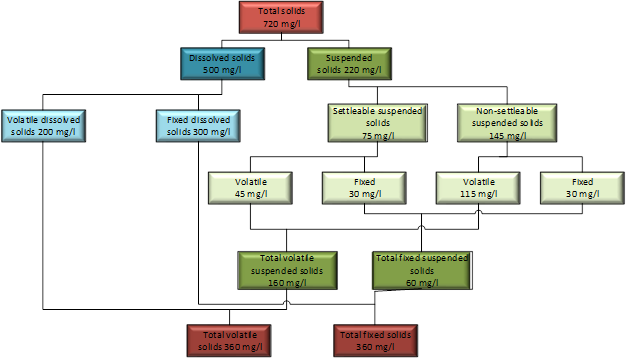
\includegraphics[scale=0.8]{WastewaterSolids}\\
					\caption{Typical Wastewater Solids Concentrations}
				\end{center}
				\end{figure}
% % 			\end{enumerate}
				
\section{Nutrients}\index{Nutrients}	
% 			\begin{snugshade*}
% 				\item \noindent\textsc{Nutrients}
% 			\end{snugshade*}	
			\begin{itemize}
				\item Plant nutrients - nitrogen and phosphorous, present in wastewater effluent discharge, promote growth of plant and algal matter in the receiving waters causing destruction of the normal aquatic life mainly due to oxygen depletion - eutrophication.
				      
				\item Because of the potential impacts of the presence of these nutrients in wastewater effluent on the receiving waters,  limits on the levels of these nutrients is typically stipulated in the treatment plant's wastewater discharge permit.
				      
				\item Typically, conventional secondary treatment processes are designed primarily remove the organics from the wastewater.  Secondary treatment process designed to additionally remove nutrients is deemed as tertiary or advanced treatment is termed as Biological Nutrient Removal (BNR).
			\end{itemize}
	\subsection{Nitrogen}\index{Nitrogen}				
% 			\begin{enumerate}%@@@@@@@@@@@@@@@@@@%
% 				\definecolor{shadecolor}{RGB}{220,220,220}
% 				\begin{snugshade*}
% 					\item \noindent\textsc{Nitrogen}%@@@@@@@@@@@@@@@@@@%
% 				\end{snugshade*}

	\subsubsection{Forms of nitrogen}\index{Forms of nitrogen}	
% 				\begin{itemize}
% 					\item Forms of nitrogen:\\
					      \begin{itemize}
					      	\item About 60\% of nitrogen in wastewater is present as ammonia nitrogen (about 60\%).  The ammonium nitrogen is present either in the form of ammonia (NH$_3$ ) or as ammonium (NH$_4^+$ ) ion.   These two forms can rapidly change from one to the other depending on pH and temperature.  Under low pH (acidic) or neutral conditions – pH less than or equal to 7, ammonia exists mostly as ammonium.  Ammonia becomes the dominant form as the pH increases to 8 and beyond.
					      	\item The other dominant form of nitrogen, about 40\% of the total nitrogen is as organic nitrogen
					      	\item Nitrogen measured as Total Kjeldahl Nitrogen (TKN) which is the sum of the organic nitrogen and the ammonia nitrogen concentrations.  Total inorganic nitrogen is the total concentration of ammonia nitrogen, NO3-, and NO2-.   Table provides the concentrations and forms of nitrogen in wastewater.
					      \end{itemize}
					      \setlength{\arrayrulewidth}{0.7mm}
					      \setlength{\tabcolsep}{8 pt}
					      \renewcommand{\arraystretch}{0.8}
					      \begin{center}
					      \begin{figure}[!htbp]
					      	\noindent \begin{tabular}[!htbp]{ |p{6cm}|p{2.0cm}|p{2.5cm}|p{2.cm}|}
					      	\hline
					      	\multicolumn{4}{|c|}{\textbf{Forms of Nitrogen in Wastewater}} \\
					      	\hline
					      	%\thead{A Head} & \thead{A Second \\ Head} & \thead{A Third \\ Head} \\
					      	%\hline%
					      	
					      	\hspace{1.8 cm}Forms of Nitrogen & \hspace{0.25 cm} Formula & \hspace{.4 cm} Found in & \hspace{.4 cm} Typical \newline \hspace{.2 cm}Concentration\\
					      	\hline
					      	\small Ammonia/Ammonium & \small NH$_3$/NH$_4^{\enspace +}$ &  \small Influent wastewater & 30-50 mg/l\\
					      	
					      	Total Kjeldahl Nitrogen \newline  \small (Ammonia/Ammonium + Organic Nitrogen) &  \small TKN &  \small Wastewater \newline  \small effluent  & 30-60 mg/l \\
					      	
					      	\small Total Inorganic Nitrogen \newline  \small (Ammonia/Ammonium + Nitrite + Nitrate) & \small TIN &  \small  Wastewater \newline  \small effluent  & 1-40 mg/l \\
					      	
					      	\small Nitrate  & $NO_3^{\enspace -}$ &  \small Nitrified effluent &  \small 1-35 mg/l \\
					      	
					      	\small Nitrate  &  $NO_2^{\enspace -}$ &  \small Partially nitrified effluent &  \small 0.1-2 mg/l \\
					      	
					      	\hline
					      	\end{tabular}
					      	\caption{Forms of Nitrogen}
					      	\end{figure}
					      \end{center}
					      
		\subsection{Phosphorous}\index{Phosphorous}			
		\subsubsection{Forms of phosphorous}\index{Forms of phosphorous}
					      \begin{itemize}
					      	\item The principal forms are organically bound phosphorus, polyphosphates, and orthophosphates.
					      	\item Organically bound phosphorus originates from body and food waste and, upon biological decomposition of these solids, is converted to orthophosphates. 
					      	\item Polyphosphates originate from synthetic detergents and are hydrolyzed to orthophosphates. Thus, the principal form of phosphorus in wastewater is assumed to be orthophosphates, although the other forms may exist. Orthophosphates consist of the negative ions PO$_4$$^{3-}$, HPO$_4$$^{2-}$, and H$_2$PO$_4$ $^-$.  These may form chemical combinations with cations (positively charged ions).
					      \end{itemize}

\section{Oil and Grease}\index{Oil and Grease}	
			Fats, oil and grease in wastewater originate from homes, food establishments and industries.
			\begin{itemize}
				\item Oil and grease content of wastewater is established in the laboratory by extracting it with a solvent - \textit{n}-hexane.  The concentration of oil and grease is reported in mg/l and typical oil and grease content of wastewater ranges from 80 - 120 mg/l
				\item Presence of excessive oils and grease could potentially impact the secondary treatment process
				\item Oils and grease are removed as floatables in primary treatment and sent with the sludge to the digesters
			\end{itemize}
		



\section{Wastewater Parameters}\index{Wastewater Parameters}			
		Laboratory and field tests are conducted to measure parameters which are critical for monitoring and controlling treatment.  The following are the key parameters that are measured.	
			
\subsection{pH}\index{pH}	
			\hl{pH is a measure of the hydrogen ion (H$^+$) content or the acidity or basicity of a solution.}  pH impacts the chemical and micribiological elements of wastewater treatment processes and thus pH measurement and control is critical.
			\begin{itemize}
				\item Pure water dissociates into equal concentration of hydrogen ions and hydroxide ions:\\ 
				      $H_2O \rightarrow H^+ + OH^-$.
				\item The H$^+$ are responsible for acidic properties and the OH$^-$ ions for the basic properties.  
				\item pH is the inverse of H$^+$ concentration; pH increases when the concentration of H$^+$ decreases relative to the concentration of OH-. 
				\item pH scale ranges from 0 – 14. When the concentration of both H$^+$ and OH$^-$ are equal, as in pure water, it is considered neutral and its pH is 7.0.  \item If the pH of a sample solution is below 7.0, the sample is termed acidic and is alkaline or basic if its pH is above 7.0. 
				\item Each change of 1 pH unit represents a 10 fold change in concentration.  For example, a sample with a pH of 2.0 is 1000 times more acidic than a sample with a pH of 5.0. 
				\item pH is measured by an electrode that is sensitive only to H$^+$ or using a pH strip which is essentially an adsorbent paper which is pre-impregnated with chemicals which change color under different H$^+$ concentrations.
				\item Most organisms involved in biological wastewater treatment processes do well within a a narrow range of pH near neutral (pH of 7).			
			\end{itemize}
			
\subsection{Oxidation Reduction Potential (ORP)}\index{Oxidation Reduction Potential (ORP)}			
			ORP is a measure of the potential of a wastewater to allow for microbiological oxidation and reduction reactions.\\
			An example of wastewater treatment process where microbiological oxidation involved include the activated sludge process.  Whereas, anaerobic digestion is a microbiological reduction based process.
			\begin{itemize}
				\item ORP value is measured in millivolts (mV), using an electrochemical probe
				\item The measured ORP value provides an indication of the potential of oxidation and reduction reactions in that sample.
				\item A higher positive ORP is indicative of oxidation potential of the wastewater whereas a negative ORP value indicates potential for a reduction reaction to occur.
				\item ORP measurements are used for controlling treatment processes including nitrification, odor control and disinfection.  For example, in the disinfection process utilizing chlorine (bleach), ORP measurements provides the strength of the oxidation potential of chlorine present in the wastewater being disinfected.  This measurement is used for precisely controlling the chlorine dosing.  The proper chlorine control results in optimizing chlorine dosing which reduces potential toxicity issues and dechlorination costs.
			\end{itemize}
			Typical ORP applications include the following processes and process elements
			
			
			\setlength{\arrayrulewidth}{0.3mm}
			\setlength{\tabcolsep}{8 pt}
			\renewcommand{\arraystretch}{0.8}
			\begin{center}
				\begin{tabular}{ |p{9.5cm}|p{4.0cm}|}
					\hline
					\multicolumn{2}{|c|}{\textbf{Typical Wastewater Process ORPs}} \\
					\hline
					
					\hline
					\small Collections	Sulfide formation                                & \small -50 to -250 mV  \\
					\small Influent wastewater                                          & \small - 200 mV        \\
					\small Activated sludge	cBOD degradation with free molecular oxygen & \small +50 to +250 mV  \\
					\small Biological phosphorous removal                               & \small +25 to +250 mV  \\
					\small Denitrification                                              & \small +50 to -50 mV   \\
					\small Anaerobic Digestion: Acid formation (Acidogenesis)           & \small -100 to -225 mV \\
					\small Anaerobic Digestion: Methane production (Methanogenesis)     & \small -75 to -400 mV  \\
					\hline
				\end{tabular}
				
			\end{center}
			
\subsection{Alkalinity}\index{Alkalinity}	
			\begin{itemize}
				\item \hl{Alkalinity is the ability of a water to neutralize acids.}  
				\item During certain wastewater treatment processes including anaerobic digestion, acids are generated as a result of microbiological activity.  The bacteria and other biological entities which play an active role in wastewater treatment are most effective at a neutral to slightly alkaline pH of 7 to 8.  In order to maintain these optimal pH conditions for biological activity there must be sufficient alkalinity present in the wastewater to neutralize acids generated by the active biomass.
				\item This ability to maintain the proper pH in the wastewater as it undergoes treatment is the reason why alkalinity is so important to the wastewater industry.
				\item The alkalinity is due to the presence of acid neutralizing bases in the water including the hydroxyl (OH$^-$), carbonate (CO$_3$$^-$) and bicarbonate (HCO$_3$$^-$)  ions.  These ions are of mineral origin and are also formed from carbon dioxide which comes from the atmosphere and from the microbial decomposition of organic material.  The resistance to pH change of the water will continue until all the alkalinity contributing ions are neutralized.  
				\item The pH of a water serves as a guide to the types of alkalinity present in the water but is unrelated to the alkalinity content of a water.  Important Note:  Alkalinity is a measure of the ability to neutralize acids whereas a solution is termed alkaline (or basic) if its pH greater than 7. 
				\item Alkalinity is expressed as milligrams per liter of CaCO$_3$
			\end{itemize}
			
\subsection{Dissolved Oxygen}\index{Dissolved Oxygen}	
			\begin{itemize}
				\item Dissolved oxygen (DO) is the concentration of oxygen dissolved in the wastewater sample and is typically measured in the field using a DO probe.  A titration based Winkler Test is used in the laboratory
				\item The \hl{presence of oxygen indicates an aerobic environment} where dissolved, free oxygen is available for aerobic microorganisms to live, BOD removal in the activated sludge process occurs as a result of the activity of aerobic bacteria.  The absence of DO indicates that the environment or condition is either anoxic or anaerobic.  
				\item \hl{In an anoxic environment, free oxygen is not present, but oxygen is available from its combined  forms - nitrate (NO$_3$ $^-$) and sulfate (SO$_4$ $^-$)} for the the consumption of microorganisms.  Example of an anoxic process is denitrification.  In denitrification, the anoxic bacteria in the presence of food (cBOD) consume the combined oxygen in nitrates (NO$_3$ $^-$ ) and convert it to nitrogen gas.
				\item \hl{The complete absence of oxygen including free and combined oxygen is an anaerobic environment.}
				\item Microorganisms are termed as obligate aerobes if they cannot survive without free oxygen.  Facultative aerobes are microorganisms which can survive in both aerobic and anaerobic environments.  
			\end{itemize}
			
\subsection{Microbiological testing and monitoring}\index{Microbiological testing and monitoring}	
			
			Microbiological testing and monitoring is conducted as part of the wastewater treatment for two main reasons:
			\begin{enumerate}[1.]
				\item Heterotrohic (organisms that consume organic material) microbes are responsible for the biological wastewater treatment processes - secondary treatment process, digestion and nutrient removal; and
				\item Pathogens - agents that cause disease are present in wastewater effluent.
			\end{enumerate}

\begin{itemize}
				
				\item Microbiological testing related to monitoring and troubleshooting biological wastewater treatment\\
				
				Microbes involved in biological wastewater treatment processes include:\\
				\begin{itemize}
					\item Fungi - Filamentous fungi occasionally bloom in activated sludge processes due to low pH or nutrient deficiency and cause problems with the settleability.
					\item Protozoa - Protozoas play a important role in the secondary treatment process.  Common protozoas in the activated sludge process include:
					      \begin{itemize}
					      	\item Amoeba
					      	\item Flagellate
					      	\item Cilliate
					      \end{itemize}
					\item Rotifers
					\item Nematodes
					\item Bacteria - Bacteria is the predominant microorganism responsible for the biological wastewater water treatment.  
				\end{itemize}
				\begin{itemize}
					\item The effectiveness of the biological wastewater treatment processes is primarily due to the presence of a microbial ecosystem with a right balance of populations of different microbial species.
					\item Methods used for monitoring the microbial composition include direct monitoring using a light microscope to see which and how many of the different microbial species are present - typically used for activated sludge process.
					\item Indirect method includes monitoring other parameters such as pH and alkalinity which are influenced by microbiological activity.
					\item The microbial monitoring ensures process stability and helps identify potential process upset conditions caused by changes to the microbial population due to other external factors - toxicty, organic loading, temperature etc.
				\end{itemize}

\item Microbiological testing related to monitoring and controlling pathogens in treated wastewater effluent\\

	
				Pathogens in wastewater belong to the following groups:
				\begin{itemize}
					\item Bacteria:  Although, bacteria is present in large numbers in feces, pathogenic or bacteria are present only because of an infection and this pathogenic bacteria can potentially spread the infection to other healthy individuals.  Disease spread by pathogenic bacteria include diarrhea, cholera and typhoid among many others.
					      
					\item Viruses: A large number of viruses may infect humans and are present in feces.  These include enteroviruses (including polioviruses), hepatitis A virus, reoviruses and diarrhea-causing viruses (especially rotavirus).
					      
					\item Protozoa:  Many species of protozoa can infect humans and cause diarrhoea and dysentery. Girardia which casues diarrheal illness is an example of a protozoan pathogen
					      
					\item Helminths:  These are parasitic worms that can infect humans and are transmitted to others through its eggs or larval forms
					      
				\end{itemize}
				
				\begin{itemize}
					\item As one of the main reasons for treating wastewater is to protect public health, microbiological/pathogen testing of the wastewater effluent and the surface water impacted by the wastewater discharge is conducted to meet the requirements of a wastewater discharge permit, to monitor the pathogen impact of treated wastewater discharge and assess the level of contamination of a public body of water.
					\item The bacteriological tests involves detection and quantification of one or more of the following bacteria:  total coliforms, fecal coliforms, E. Coli, and Enterococcus.  
					      \begin{itemize}
					      	\item The main reason why these bacteria such as coliforms and enterococcus are used \hl{as it is not practical to detect and quantify all pathogens associated with wastewater.}  
					      	\item These selected bacteria originate from feces and indicate fecal contamination and thus serve as an indicator organisms for pathogens of wastewater origin.  
					      	\item Also, they are abundant, potentially less harmful, and easy to detect.  E. coli has been shown to be a better predictor of the potential for impacts to human health and therefore many newer wastewater discharge permits require E. Coli testing in lieu of fecal coliform testing requirements.
					      \end{itemize}
					\item The microbiological test sample is always collected as a grab in a clean, sterile borosilicate glass or plastic bottle containing sodium thiosulfate. 
					      \begin{itemize}
					      	\item Sodium thiosulfate is added to remove residual chlorine which will kill coliforms during transit. 
					      	\item If the sample is not preserved or maintained under proper conditions until the test is conducted in the laboratory, the test would provide erroneous results.
					      	\item Samples must be refrigerated if they cannot be analyzed within 1 hour of collection and must be handled with care to prevent contamination and adverse conditions such as prolonged exposure to direct sunlight.
					      	\item The maximum holding time for state or federal permit reporting purposes is 6 hours. 
					      \end{itemize} 
					\item As it is not possible to exactly quantify the number of bacteria present, a statistical based - \hl{Most Probable Number (MPN)} approach is utilized.  The methods for wastewater bacteriological tests include:  multiple-tube fermentation technique, membrane filtration and quanti-tray testing. 
				\end{itemize}
			\end{itemize}

\subsection{Specific Gravity}\index{Specific Gravity}				
			\begin{itemize}
				\item Specific gravity is a term to express the weight of a solution with respect to that of water
				\item Water weighs 1 kg/L or 8.34 lbs/gallon or 62.4 lbs/ft$^3$
				\item A solution with a specific gravity of 1.2 will weigh 1.2 times the same volume of water.  1 L of that solution will weigh ( 1.2 kg )/L  or  ( 1.2*8.34=10lbs )/gallon.
				\item Typically wastewater and the associated unthickened sludge, for all practical purposes is assumed to have a specific gravity of 1 - implying 8.34 lbs/gallon.
				\item Specific gravity is typically used for calculations related to chemicals used in wastewater treatment.
			\end{itemize}
			
\section{Wastewater Sampling}\index{Wastewater Sampling}
		\begin{itemize}
			\item Field or laboratory measurement of a certain parameter is critical in wastewater treatment operations to obtain information about wastewater characteristics in order to either characterize a wastewater stream, or to monitor a treatment process or for permit compliance.  
			\item A sample is a small part of the whole representing the whole.  Thus, a sample needs to be such that it truly represents the entire population – which in a wastewater operations could be either a wastewater stream, wastewater solids or a chemical used.
		\end{itemize}
		
\subsection{Sampling Methods}\index{Sampling Methods}
\subsubsection{Grab Samples}\index{Grab Samples}
				\begin{itemize}
					\item A grab sample is a sample collected at a specific spot at a site over a short period of time.  
					\item Grab sampling allows for instantaneous analysis of parameters such as pH, dissolved oxygen, chlorine residual, temperature and other parameters which change rapidly with time.
					\item A grab sample represents a snapshot of space and time of a process stream.
					\end{itemize}
\subsubsection{Composite Samples}\index{Composite Samples}
				\begin{itemize}
					\item A composite sample is a collection of discrete samples are combined over a certain period or space and therefore represent the average performance of a wastewater treatment plant or a process during the collection period.\\  
					\item Composite sampling can be either based on:
					      
					      1. constant time interval (time proportioned sampling)\\
					      2. constant wastewater volume interval (flow-proportioned sampling), and\\
					      3. treatment process space - includes samples taken at different depths\\
					      
					\item Composite samples are typically collected using automated samplers which can be programmed to collect samples at pre-established time intervals – for time proportional sampling.
					\item Time and space composite samples are collected by adding equal volumes of samples collected from different times or locations.  
					\item Flow proportional composite samples comprise of volume of each subsample based on flow.\\  
				\end{itemize}
				
			\begin{center}
				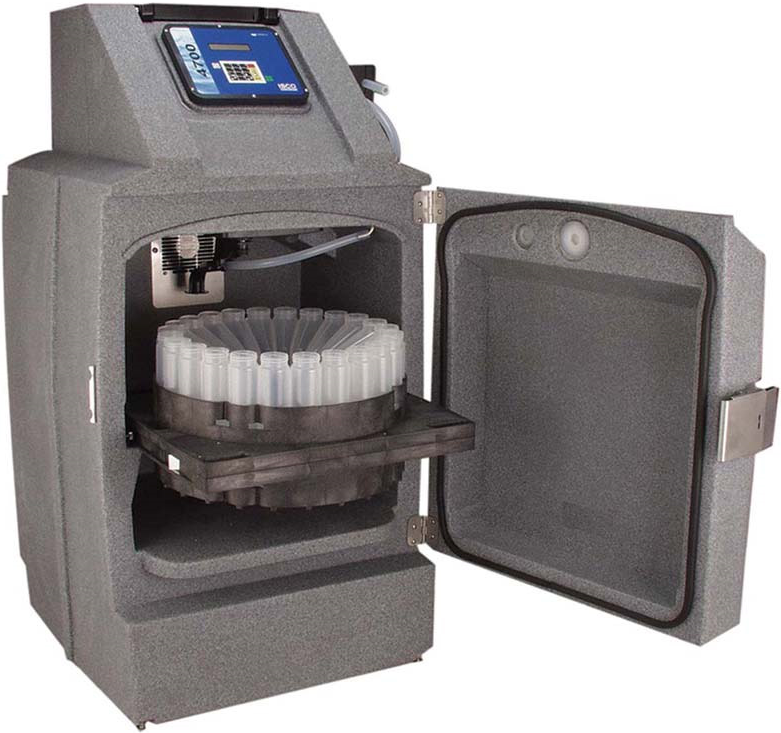
\includegraphics[scale=0.2]{Autosampler} \hspace{2cm} 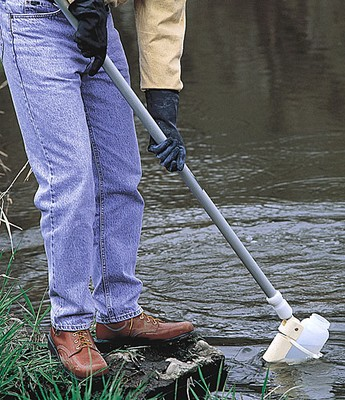
\includegraphics[scale=0.37]{Grabsampler}\\
			\end{center}
			\hspace{2.3cm} Automated Sampler \hspace{2.0cm} \parbox{\textwidth}{Grab Sampling Using a Long Handle Dipper}\\

\subsubsection{Sampling Precautions and Protocols}\index{Sampling Precautions and Protocols}
			\begin{itemize}
				\item Samples should represent the major portion of the process or the process stream and should be taken from places where the mixing is thorough, avoiding dead spots and areas of heavier or lighter loadings. 
				\item The collected sample is invariably exposed to conditions very different from the original source and is subject to change due to chemical and microbiological activity.  
				\item Thus, in order to ensure integrity of sample, sample preservation techniques specific to the analysis to be performed is needed.  
				      \begin{itemize}
				      	\item The preservation technique should not only allow for stabilizing the parameter to be analyzed, it should also not interfere with the analyses.  
				      	\item The common preservation techniques involve use of proper containers, temperature control, addition of chemical preservatives, and observance of the recommended maximum sample holding time.
				      \end{itemize}
			\end{itemize}

\section{Data Reporting}\index{Data Reporting}	
		\begin{itemize}
			\item Arithmetic mean is typically calculated for reporting data where multiple samples have been collected and analyzed for the same process stream at different times and for reporting average value over a certain time period – daily, monthly etc.\\ \item Arithmetic mean mathematically is calculated by adding all the result values and dividing by the total number of data points.\\
		\end{itemize}
		Mathematically the arithmetic mean is represented as:\\
		$$\bar{x}=\dfrac{\sum_{i=1}^{n} x^i}{n} = \dfrac{x_1+x_2+x_3...x_n}{n}$$
		For example:\\
		Arithmetic mean of the following set of data points:  200, 304, 250, 400 is calculated as:\\
		\vspace{10pt}
		Arithmetic Mean = $\dfrac{200 + 302 + 250 + 400}{4}= 288$\\
		\vspace{10pt}
		For data sets for analysis such as fecal coliform could include values which vary by several orders of magnitudes, using the arithmetic mean to report the average value is not appropriate as the lower or higher values would bias the calculated mean.\\
		\vspace{10pt}
		For example, consider a data set with values:  260, 300, 500, 5,000, 320 and 200.\\
		\vspace{10pt}
		The arithmetic mean = $\dfrac{260+300+500+5,000+320+200}{6} = 3,444$\\
		Here the 5000 value completely skews the arithmetic mean.
		
		Therefore, for such tests, the geometric mean calculation is used for reporting the average value.\\
		
		
		Mathematically a geometric mean is represented as:\\
		$$\Bigg(\prod_{i=a}^n\Bigg)^{\dfrac{1}{n}}=\sqrt[n]{a_1*a_2*a_3...a_n}$$
		 
		Calculation method:\\
		1.	Find the product of all the data points (analogous to first calculating the sum of all the data points when calculating the arithmetic mean)\\
		260*300*500*5,000*320*200 = 12,480,000,000,000,000\\
		2.	Raise the product to the inverse of the number of data points\\
		(*Using the power function of a scientific calculator)\\
		Here n (\# data points) = 6 $\implies$ geometric mean = $(12,480,000,000,000,000)^{\dfrac{1}{6}}   = 482$

\end{document}
%% This is an example of theorems.
%\part{Module 7}
%\input{WATR080 Module7.tex}
% \subsection{Several equations}\index{Theorems!Several Equations}
% This is a theorem consisting of several equations.

% \begin{theorem}[Name of the theorem]
% In $E=\mathbb{R}^n$ all norms are equivalent. It has the properties:
% \begin{align}
% & \big| ||\mathbf{x}|| - ||\mathbf{y}|| \big|\leq || \mathbf{x}- \mathbf{y}||\\
% &  ||\sum_{i=1}^n\mathbf{x}_i||\leq \sum_{i=1}^n||\mathbf{x}_i||\quad\text{where $n$ is a finite integer}
% \end{align}
% \end{theorem}

% \subsection{Single Line}\index{Theorems!Single Line}
% This is a theorem consisting of just one line.

% \begin{theorem}
% A set $\mathcal{D}(G)$ in dense in $L^2(G)$, $|\cdot|_0$. 
% \end{theorem}

% %------------------------------------------------

% \section{Definitions}\index{Definitions}

% This is an example of a definition. A definition could be mathematical or it could define a concept.

% \begin{definition}[Definition name]
% Given a vector space $E$, a norm on $E$ is an application, denoted $||\cdot||$, $E$ in $\mathbb{R}^+=[0,+\infty[$ such that:
% \begin{align}
% & ||\mathbf{x}||=0\ \Rightarrow\ \mathbf{x}=\mathbf{0}\\
% & ||\lambda \mathbf{x}||=|\lambda|\cdot ||\mathbf{x}||\\
% & ||\mathbf{x}+\mathbf{y}||\leq ||\mathbf{x}||+||\mathbf{y}||
% \end{align}
% \end{definition}

% %------------------------------------------------

% \section{Notations}\index{Notations}

% \begin{notation}
% Given an open subset $G$ of $\mathbb{R}^n$, the set of functions $\varphi$ are:
% \begin{enumerate}
% \item Bounded support $G$;
% \item Infinitely differentiable;
% \end{enumerate}
% a vector space is denoted by $\mathcal{D}(G)$. 
% \end{notation}

%------------------------------------------------

% \section{Remarks}\index{Remarks}

% This is an example of a remark.

% \begin{remark}
% The concepts presented here are now in conventional employment in mathematics. Vector spaces are taken over the field $\mathbb{K}=\mathbb{R}$, however, established properties are easily extended to $\mathbb{K}=\mathbb{C}$.
% \end{remark}

% %------------------------------------------------

% \section{Corollaries}\index{Corollaries}

% This is an example of a corollary.

% \begin{corollary}[Corollary name]
% The concepts presented here are now in conventional employment in mathematics. Vector spaces are taken over the field $\mathbb{K}=\mathbb{R}$, however, established properties are easily extended to $\mathbb{K}=\mathbb{C}$.
% \end{corollary}

%------------------------------------------------

% \section{Propositions}\index{Propositions}

% This is an example of propositions.

% \subsection{Several equations}\index{Propositions!Several Equations}

% \begin{proposition}[Proposition name]
% It has the properties:
% \begin{align}
% & \big| ||\mathbf{x}|| - ||\mathbf{y}|| \big|\leq || \mathbf{x}- \mathbf{y}||\\
% &  ||\sum_{i=1}^n\mathbf{x}_i||\leq \sum_{i=1}^n||\mathbf{x}_i||\quad\text{where $n$ is a finite integer}
% \end{align}
% \end{proposition}

% \subsection{Single Line}\index{Propositions!Single Line}

% \begin{proposition} 
% Let $f,g\in L^2(G)$; if $\forall \varphi\in\mathcal{D}(G)$, $(f,\varphi)_0=(g,\varphi)_0$ then $f = g$. 
% \end{proposition}

%------------------------------------------------

% \section{Examples}\index{Examples}

% This is an example of examples.

% \subsection{Equation and Text}\index{Examples!Equation and Text}

% \begin{example}
% Let $G=\{x\in\mathbb{R}^2:|x|<3\}$ and denoted by: $x^0=(1,1)$; consider the function:
% \begin{equation}
% f(x)=\left\{\begin{aligned} & \mathrm{e}^{|x|} & & \text{si $|x-x^0|\leq 1/2$}\\
% & 0 & & \text{si $|x-x^0|> 1/2$}\end{aligned}\right.
% \end{equation}
% The function $f$ has bounded support, we can take $A=\{x\in\mathbb{R}^2:|x-x^0|\leq 1/2+\epsilon\}$ for all $\epsilon\in\intoo{0}{5/2-\sqrt{2}}$.
% \end{example}

% \subsection{Paragraph of Text}\index{Examples!Paragraph of Text}

% \begin{example}[Example name]
% \lipsum[2]
% \end{example}

%------------------------------------------------

% \section{Exercises}\index{Exercises}

% This is an example of an exercise.

% \begin{exercise}
% This is a good place to ask a question to test learning progress or further cement ideas into students' minds.
% \end{exercise}

%------------------------------------------------

% \section{Problems}\index{Problems}

% \begin{problem}
% What is the average airspeed velocity of an unladen swallow?
% \end{problem}

%------------------------------------------------

% \section{Vocabulary}\index{Vocabulary}

% Define a word to improve a students' vocabulary.

% \begin{vocabulary}[Word]
% Definition of word.
% \end{vocabulary}

%----------------------------------------------------------------------------------------
%	PART 3
%----------------------------------------------------------------------------------------

%\part{Analysis and Testing}

%----------------------------------------------------------------------------------------
%	CHAPTER 3
%----------------------------------------------------------------------------------------
%\input{WastewaterAnalysisandLaboratoryMethods.tex}
% \chapterimage{chapter_head_1.pdf} % Chapter heading image

% \chapter{Presenting Information}

% \section{Table}\index{Table}

% \begin{table}[h]
% \centering
% \begin{tabular}{l l l}
% \toprule
% \textbf{Treatments} & \textbf{Response 1} & \textbf{Response 2}\\
% \midrule
% Treatment 1 & 0.0003262 & 0.562 \\
% Treatment 2 & 0.0015681 & 0.910 \\
% Treatment 3 & 0.0009271 & 0.296 \\
% \bottomrule
% \end{tabular}
% \caption{Table caption}
% \label{tab:example} % Unique label used for referencing the table in-text
% %\addcontentsline{toc}{table}{Table \ref{tab:example}} % Uncomment to add the table to the table of contents
% \end{table}

% Referencing Table \ref{tab:example} in-text automatically.

% %------------------------------------------------

% \section{Figure}\index{Figure}

% \begin{figure}[h]
% \centering
\includegraphics[scale=0.5]{placeholder.jpg}
% \caption{Figure caption}
% \label{fig:placeholder} % Unique label used for referencing the figure in-text
% %\addcontentsline{toc}{figure}{Figure \ref{fig:placeholder}} % Uncomment to add the figure to the table of contents
% \end{figure}

% Referencing Figure \ref{fig:placeholder} in-text automatically.

%----------------------------------------------------------------------------------------
%%	BIBLIOGRAPHY
%%----------------------------------------------------------------------------------------
%
%\chapter*{Bibliography}
%\addcontentsline{toc}{chapter}{\textcolor{ocre}{Bibliography}} % Add a Bibliography heading to the table of contents
%
%%------------------------------------------------
%
%\section*{Articles}
%\addcontentsline{toc}{section}{Articles}
%\printbibliography[heading=bibempty,type=article]
%
%%------------------------------------------------
%
%\section*{Books}
%\addcontentsline{toc}{section}{Books}
%\printbibliography[heading=bibempty,type=book]
%
%%----------------------------------------------------------------------------------------
%%	INDEX
%%----------------------------------------------------------------------------------------
%
%\cleardoublepage % Make sure the index starts on an odd (right side) page
%\phantomsection
%\setlength{\columnsep}{0.75cm} % Space between the 2 columns of the index
%\addcontentsline{toc}{chapter}{\textcolor{ocre}{Index}} % Add an Index heading to the table of contents
%\printindex % Output the index

%----------------------------------------------------------------------------------------

\end{document}
